%\title{Math208book-v3Corr}
\documentclass[letterpaper, twoside]{tufte-book}
% symmetric,notoc options output left-right/even-odd format for traditional print book. May make a mess!
% justified option right justifies left & right margins of body box. May cause over hyphenation.
% Use just twoside to get Tufte's design for print books.

%% Draft only packages
%\usepackage{showframe}

% Utility packages
\usepackage{standalone}
\usepackage{etoolbox}
\newtoggle{tufte}
\toggletrue{tufte}
\usepackage{amsmath}
\usepackage{amsthm}
\usepackage{thmtools}
\usepackage{amssymb}
\usepackage{geometry}
\usepackage{setspace}
\usepackage{manfnt}
\usepackage{cancel}
%\usepackage{relsize}

\usepackage{graphicx}

\usepackage{algpseudocode}
\usepackage{algorithm}
\renewcommand{\algorithmicrequire}{\textbf{Input:}}
\renewcommand{\algorithmicensure}{\textbf{Output:}}

%\usepackage{pseudocode}

%\makeatletter
%\def\BState{\State\hskip-\ALG@thistlm}
%\makeatother

\usepackage{enumerate}
\usepackage{listings}
\usepackage{booktabs}
\usepackage{tabularx}

\usepackage{hyperref}
\usepackage{xparse}
\usepackage{xspace}
\usepackage[inline]{enumitem}
\usepackage{multirow}
\usepackage{todonotes}
\usepackage{dcolumn}
\usepackage{array}
\usepackage{booktabs}
\usepackage{colortbl, xcolor}
\usepackage{longtable}
\usepackage{tabu}
\usepackage{natbib}
\usepackage{python}

\usepackage[page,toc]{appendix}

\usepackage{tikz}
\usepackage{pgfplots}
\usepackage{pgfplotstable}
\usepackage{mathdots}
\usepgflibrary{fpu}
\usetikzlibrary{positioning,chains,fit,shapes,calc,arrows,patterns}
\usepackage{tkz-graph}
\usetikzlibrary{arrows, petri, topaths}
\usepackage{tkz-berge}
\usepackage[all]{xy}

\usepackage{pdfpages} % to use \includepdf in chapter 

\hypersetup{colorlinks=true}

\graphicspath{./Graphics}

%thmtools
\declaretheorem[numberwithin=chapter,name=Theorem]{thm}
\declaretheorem[name=Lemma,sibling=thm]{lem}
\declaretheorem[name=Corollary,sibling=thm]{corollary}
\declaretheorem[name=Definition,sibling=thm,style=definition]{defn}
\declaretheorem[name=Proposition,sibling=thm]{proposition}
\declaretheorem[name=Example,sibling=thm]{exmp}
%\declaretheorem[name=Exercise,sibling=thm]{exer}
\declaretheorem[numberwithin=chapter,name=Exercise]{exer}
\declaretheorem[numberwithin=chapter,name=Problem]{prob}
\declaretheorem[name=History,sibling=thm]{history}
\declaretheorem[name=Question,sibling=thm]{question}
\declaretheorem[name=Remark,sibling=thm]{remark}
\declaretheorem[name=Notation,numbered=no]{notation}
\declaretheorem[name=Theorem,sibling=thm,thmbox=L]{boxthm}
\declaretheorem[name=Argument,numbered=no]{argu}
\declaretheorem[name={\itshape Solution},numbered=no]{soln}

\let\proof\relax
\def\qedsymbol{\square}% PLEASE NOTE: this is in the AMS symbols font.
\declaretheorem[name=Proof,style=thm,numbered=no,qed=\qedsymbol]{proof} %this uses Richard's \clubsuit, not Halmos Tombstone: \square!
\declaretheorem[name=Counterexample,style=thm,numbered=no,qed=\spadesuit]{cntrxmpl}

\DeclareMathOperator*{\argmax}{arg\,max}
\DeclareMathOperator*{\argmin}{arg\,min}
\DeclareMathOperator*{\aff}{aff}
\DeclareMathOperator*{\rint}{rint}
\DeclareMathOperator*{\lev}{lev}
\DeclareMathOperator*{\tr}{tr}
\DeclareMathOperator*{\interior}{int}
\DeclareMathOperator*{\epi}{epi}
\DeclareMathOperator*{\dom}{dom}
\DeclareMathOperator*{\vecspan}{span}
\DeclareMathOperator*{\con}{con}
\DeclareMathOperator*{\cl}{cl}
\DeclareMathOperator*{\grad}{\nabla}
\DeclareMathOperator*{\crit}{crit}
\DeclareMathOperator*{\diag}{diag}
\DeclareMathOperator*{\res}{Res}
\DeclareMathOperator*{\boundary}{boundary}
\DeclareMathOperator*{\range}{range}
\DeclareMathOperator*{\Tr}{Tr}
\DeclareMathOperator*{\sign}{sign}
\DeclareMathOperator{\lcm}{lcm}
%\setlist[enumerate]{label=(\alph*)}
\setlist[enumerate]{label=(\arabic*)}

%%%%%%%%%%%%%%%%%%%%%%%%%% Format Exercises and Answers %%%%%%%%%%%%%%%%%%%%%%%%%%%%
\newlist{exercises}{enumerate}{1}
\setlist[exercises]{label=Ex. \arabic*}
%%%%%%%%%%%%%%%%%%%%%% Answers Package %%%%%%%%%%%%%%%%%%%%%%%%%%%%%%%%%%
\usepackage{answers}  %Put solutions in an appendix
%\usepackage[nosolutionfiles]{answers} %Put solutions with exercises
\Newassociation{sol}{Solution}{ans}
\renewcommand{\Solutionlabel}[1]{\textbf{#1.}}% Make the period appear after soln number
% Fix the exercise number in a solution after a tasks environment in the exercies (uses etoolbox macro AtBeginEnvironment)
\AtBeginEnvironment{sol}{\addtocounter{exer}{-1}\refstepcounter{exer}}
%\AtBeginEnvironment{sol}{\renewcommand{\Solutionlabel}[1]{\textbf{\theexer.}}} %% My first attempt. It works, but is not elegant.
\newtheorem{exc}{}
\newenvironment{ex}{\begin{exc}\normalfont}{\end{exc}}


% Use multicol package to format solutions in columns,
% writing the multicol environment into the answer file
%\newenvironment{solnmulticols}[1]%
%{\Writetofile{ans}{\string\begin{multicols}{#1}}}%
%{\Writetofile{ans}{\string\end{multicols}}}%
%%%%%%%%%%%%%%%%%%%%%%%%%%%%%%%%%%%%%%%%%%%%%%%%%%%%%%%%%%%%%%%%%%%

\usepackage{tasks}


\setcounter{secnumdepth}{2}
\setcounter{tocdepth}{2}
\onehalfspacing


% Book metadata
\title{Math208:\\Discrete\\Mathematics %
\thanks{Thanks to UND Math.}}
\author[UND Math Book Developers]{UND Mathematics}
\publisher{Department of Mathematics\\The University of North Dakota}


%
% Prints the month name (e.g., January) and the year (e.g., 2008)
\newcommand{\monthyear}{%
  \ifcase\month\or January\or February\or March\or April\or May\or June\or
  July\or August\or September\or October\or November\or
  December\fi\space\number\year
}


% % macros from Richard's mathmacs.tex, augmented with some extras
\def \U {{\cal {U}}} 
\def \P {{\cal {P}}}
\def \Z {\mathbb{Z}}
\def \N {\mathbb{N}}
\def \Q {\mathbb{Q}}
\def \R {\mathbb{R}}
\def \C {\mathbb{C}}
\def \F {\mathbb{F}}
\def \ms {\medskip}
\def \ss {\smallskip}
\def \no {\noindent}
\def \vl {\overline}
\def \ub {\underbar}
\def \cl {\centerline}
\def \dl {\displaystyle}
\def \lra {\longrightarrow}
\def \iff {\longleftrightarrow}
\def \thus {{.\raise 4pt\hbox{.}.\;}}
%\def \mod {{\rm {~(mod~}}}
\def \ctrdct {\rightarrow \!\leftarrow}
\def \div {{\bf {~div~}}}
%\def \bmod #1{{~(\bf {mod~{#1}})}}
\def \qed {$\clubsuit$}
%\def \notdiv #1 #2{{#1}\kern -3pt\not|\kern 2pt{#2}}
\def\notdiv{\not|\;}
\font\Bigbf = cmr10 scaled\magstep 2
\font\sm = cmr10 scaled 900
\font\headerfont = cmti10 scaled 600
\def\LaTeX{{\rm L\kern-.36em\raise.3ex\hbox{\sc a}\kern-.15em\TeX}}

\def\doblue #1 {\color{blue}}

%%%% Make new algorithm float: algrthm, and margin algorithm float: marginalgrthm
\newcounter{algrthm}[chapter]
\newcommand\algrthmname{Algorithm}
\newcommand\listalgrthmname{List of Algorithms}

\makeatletter
\newcommand\listofalgrthms{%
  \ifthenelse{\equal{\@tufte@class}{book}}%
    {\chapter*{\listalgrthmname}}%
    {\section*{\listalgrthmname}}%
%  \begin{fullwidth}%
    \@starttoc{loa}%
%  \end{fullwidth}%
}
\renewcommand\thealgrthm
     {\ifnum \c@chapter>\z@ \thechapter.\fi \@arabic\c@algrthm}
\def\fps@algrthm{tbp}
\def\ftype@algrthm{1}
\def\ext@algrthm{loa}
\def\fnum@algrthm{\algrthmname\nobreakspace\thealgrthm}

% Main body algorithm environment
\newenvironment{algrthm}[1][htbp]
  {\begin{@tufte@float}[#1]{algrthm}{}}
  {\end{@tufte@float}}
\let\l@algrthm\l@figure
\makeatother

%%
% Margin algorithm environment
\newenvironment{marginalgrthm}[1][-1.2ex]%
  {\begin{@tufte@margin@float}[#1]{algrthm}}
  {\end{@tufte@margin@float}}

%% environments with bounding lines
\newenvironment{algo}{\begin{algrthm} \kern2pt\hrule\kern5pt\relax}
{\kern2pt\hrule\kern5pt\relax\end{algrthm}}

\newenvironment{malgo}{\begin{marginalgrthm}\begin{minipage}{\marginparwidth}\kern2pt\hrule\kern5pt\relax}
{\end{minipage}\kern2pt\hrule\kern5pt\relax\end{marginalgrthm}}

% % % % % % End definition of algrthm environments
% Generates the index
%\usepackage{makeidx}
%\makeindex

\begin{document}

% Front matter
\frontmatter

%full title page
\maketitle

%copyright page
\newpage
\begin{fullwidth}
~\vfill
\thispagestyle{empty}
\setlength{\parindent}{0pt}
\setlength{\parskip}{\baselineskip}
Copyright \copyright\ \the\year\ \thanklessauthor

\par\smallcaps{Published by \thanklesspublisher}

\par\smallcaps{~\url{http://arts-sciences.und.edu/math//}}


\noindent Copyright \copyright\  
2005, 2006, 2007, 2008, 2009, 2014, 2015, 2016, 2017 University of North Dakota Mathematics Department
\par
 Permission is granted to copy, distribute and/or modify this document
    under the terms of the GNU Free Documentation License, Version 1.2
    or any later version published by the Free Software Foundation;
    with no Invariant Sections, no Front-Cover Texts, and no Back-Cover Texts.
    A copy of the license is included in the section entitled "GNU
    Free Documentation License".

\par\textit{Third edition, First printing: \monthyear} 
\end{fullwidth}

% contents, figures and tables
\tableofcontents

\listoffigures

\listoftables

\listofalgrthms


%% dedication
%\cleardoublepage
%~\vfill
%\begin{doublespace}
%\noindent\fontsize{18}{22}\selectfont\itshape
%\nohyphenation
%Dedicated to the students of Discrete Mathematics.
%\end{doublespace}
%%\vfill
%%\vfill


\cleardoublepage
\mainmatter


% introduction
\cleardoublepage
\chapter*{Introduction}
\begin{quote}
\newthought{%
Discrete math has become increasingly important in recent years, for a number of reasons:\sidenote{\textit{The Art of Problem Solving} ~\url{http://www.artofproblemsolving.com/articles/discrete-math}}
}

\vspace*{0.25cm}
\noindent
{\large\color{blue}Discrete math is essential to college-level mathematics --- 
and beyond.}

Discrete math --- together with calculus and abstract algebra --- is one of the core
 components of mathematics at the undergraduate level. Students who learn a significant
 quantity of discrete math before entering college will be at a significant advantage
 when taking undergraduate-level math courses.

\vspace*{0.25cm}
\noindent
{\large\color{blue}Discrete math is the mathematics of computing.}

The mathematics of modern computer science is built almost entirely on discrete math,
 in particular combinatorics and graph theory. This means that in order to learn the
 fundamental algorithms used by computer programmers, students will need a solid
 background in these subjects. Indeed, at most universities, a undergraduate-level
 course in discrete mathematics is a required part of pursuing a computer science
 degree.

\vspace*{0.25cm}
\noindent
{\large\color{blue}Discrete math is very much ''real world'' mathematics.}

Many students' complaints about traditional high school math --- algebra, geometry,
 trigonometry, and the like --- is "What is this good for?" The somewhat abstract
 nature of these subjects often turn off students. By contrast, discrete math, in
 particular counting and probability, allows students --- even at the middle school
 level --- to very quickly explore non-trivial "real world" problems that are
 challenging and interesting.

%\vspace*{0.25cm}
\clearpage
\noindent
{\large\color{blue}Discre te math shows up on most middle and high school math contests.}

Prominent math competitions such as MATHCOUNTS (at the middle school level) and the
 American Mathematics Competitions (at the high school level) feature discrete math
 questions as a significant portion of their contests. On harder high school contests,
 such as the AIME, the quantity of discrete math is even larger. Students that do not
 have a discrete math background will be at a significant disadvantage in these
 contests. In fact, one prominent MATHCOUNTS coach tells us that he spends nearly
 50\% of his preparation time with his students covering counting and probability
 topics, because of their importance in MATHCOUNTS contests.

\vspace*{0.25cm}
\noindent
{\large\color{blue}Discrete math teaches mathematical reasoning and proof techniques.}

Algebra is often taught as a series of formulas and algorithms for students to memorize
 (for example, the quadratic formula, solving systems of linear equations by
 substitution, etc.), and geometry is often taught as a series of
 ''definition-theorem-proof'' exercises that are often done by rote (for example, the
 infamous ''two-column proof''). While undoubtedly the subject matter being taught is
 important, the material (as least at the introductory level) does not lend itself
 to a great deal of creative mathematical thinking. By contrast, with discrete
 mathematics, students will be thinking flexibly and creatively right out of the
 box. There are relatively few formulas to memorize; rather, there are a number
 of fundamental concepts to be mastered and applied in many different ways.

\vspace*{0.25cm}         
\noindent
{\large\color{blue}Discrete math is fun.}

Many students, especially bright and motivated students, find algebra, geometry, and even calculus dull and uninspiring. Rarely is this the case with most discrete math topics. When we ask students what their favorite topic is, most respond either ''combinatorics'' or ''number theory.'' (When we ask them what their least favorite topic is, the overwhelming response is ''geometry.'') Simply put, most students find discrete math more fun than algebra or geometry.
\end{quote}

%%
% Start the main matter (normal chapters)
\mainmatter


% Chapters
%\include{Chapters/208ch01} %Logical Connectives and Compound Propositions
\chapter{Logical Connectives and Compound Propositions}\label{ch:logic prop}


\begin{quote}
\newthought{Logic is concerned with forms of reasoning.} Since reasoning is involved in most intellectual activities, logic is relevant to a broad range of pursuits. The study of logic is essential for students of computer science. It is also very valuable for mathematics students, and others who make use of mathematical proofs, for instance, linguistics students. In the process of reasoning one makes inferences. In an inference one uses a collection of statements, the premises, in order to justify another statement, the conclusion. The most reliable types of inferences are deductive inferences, in which the conclusion must be true if the premises are. Recall elementary geometry: Assuming that the postulates are true, we prove that other statements, such as the Pythagorean Theorem, must also be true. Geometric proofs, and other mathematical proofs, typically use many deductive inferences. (Robert L. Causey)\sidenote{\url{www.cs.utexas.edu/\~rlc/whylog.htm}}
\end{quote}
 
 
\section{Propositions} 
The basic objects in logic are {\bfseries propositions}. A proposition is a statement which is either true ($T$) or
false ($F$) but not both. For example in the language of mathematics $\mathit p : 3+3=6$ is a true proposition
while  $\mathit q:2+3=6$ is a false proposition. {\itshape What do you want for lunch?} is a question, 
not a proposition. Likewise {\itshape Get lost!} is a command, not a proposition. 
The sentence {\itshape There are exactly $10^{87} + 3$ stars in the universe} is a proposition, despite the fact
that no one knows its truth value. Here are two, more subtle, examples:

\begin{enumerate}
\item {\itshape He is more than three feet tall} is not a proposition since, until we are told to whom {\itshape he}
refers, the statement cannot be assigned a truth value. The mathematical sentence $x+3 = 7$ is not a proposition for the
same reason. In general, sentences containing variables are not propositions unless some information is supplied about
the variables. More about that later however.

\marginnote{%
Sometimes a little common sense is required. For example {\itshape It is raining} 
is a proposition, but its truth value is not constant, 
and may be arguable. That is, someone might say {\itshape It is not raining, it is just drizzling},
or {\itshape Do you mean on Venus?} Feel free to ignore this sort of quibbling.
}
\item {\itshape This sentence is false} is not a proposition. It seems to be both true and false.
 In fact if is $T$ then it says it is 
$F$ and if it is $F$ then it says it is $T$. It can be dangerous using sentences that refer to themselves. 
If course, using a knife can also be dangerous, but we do use knives safely when we are careful. Likewise,
using self-referential sentences can be done safely if care is taken.
\end{enumerate}

 Simple propositions, such as {\itshape It is raining}, and {\itshape The streets are
wet}, can be combined to create more complicated propositions such as {\itshape It is
raining and the streets are not wet}. These sorts of involved propositions are
called {\bfseries compound propositions}. Compound propositions are built up from simple
propositions using a number of {\bfseries connectives} to join or modify the simple
propositions. In the last example, the connectives are {\bfseries and} which joins the
two clauses, and {\bfseries not}, which modifies the second clause.

It is important to keep in mind that since a compound proposition is,
after all, a proposition, it must be classifiable as either true or false. That
is, it must be possible to assign a truth value to any compound proposition.
There are mutually agreed upon rules to allow the determination of exactly when a
compound proposition is true and when it is false. Luckily these rules jive nicely
with common sense (with one small exception), so they are easy to remember and understand.


\section{Negation: \textbf{not}}
The simplest logical connective is  {\bfseries negation}. 
In normal English sentences, this connective is indicated by appropriately inserting  {\itshape not} in the statement, by preceding the
statement with {\itshape it is not the case that}, or for mathematical statements, by using a slanted slash.
For example, if $p$ is the proposition $2+3 = 4$, then  the negation of $p$ is denoted by the symbol
$\lnot p$ and it is the proposition  $2+3\neq 4$. In this case, $p$ is false
 and $\lnot p$ is true.  If $p$ is {\itshape It is raining}, then $\lnot p$ is {\itshape It is not raining} or even
the stilted sounding 
{\itshape It is not the case that it is raining}. 
The negation of a proposition $p$ is the proposition whose truth value is the opposite of $p$ in all cases.
The behavior of $\lnot p$ can be exhibited 
in a {\bfseries truth table}. In each row of the truth table \ref{tbl:not} we list a possible truth value of $p$ 
and the corresponding truth value of $\lnot p$.

\begin{margintable}
\begin{tabular}{@{ }c | c@{ }@{ }c}
p & $\sim$ & p\\
\hline 
T & \textcolor{red}{F} & T\\
F & \textcolor{red}{T} & F\\
\end{tabular}
\caption{Logical Negation}
\label{tbl:not}
\end{margintable}


\section{Conjunction: \textbf{and}}
The connective that corresponds to the word {\itshape and} is called {\bfseries conjunction}.  The
conjunction of $p$ with $q$ is denoted  by $p\wedge q$ and read  as {\itshape $p\hbox{ and }q$}. The conjunction of
$p$ with $q$ is declared to be true exactly when both of $p,q$ are true. It is false otherwise. This behavior
is exhibited in the truth table \ref{tbl:conjunction}. 

\begin{margintable}
\begin{tabular}{@{ }c@{ }@{ }c | c@{ }@{ }c@{ }@{ }c@{ }@{ }c@{ }@{ }c}
p & q &  & p & $\land$ & q & \\
\hline 
T & T &  & T & \textcolor{red}{T} & T & \\
T & F &  & T & \textcolor{red}{F} & F & \\
F & T &  & F & \textcolor{red}{F} & T & \\
F & F &  & F & \textcolor{red}{F} & F & \\
\end{tabular}
\caption{Logical Conjunction}
\label{tbl:conjunction}
\end{margintable}

Four rows are required in this table since when $p$ is true, $q$ may be either true or
false and  when $p$ is false it is possible for $q$ to be either true or false. Since a truth
value must be assigned to $p\land q$ in every possible case, one row in the truth table is needed
for each of the four possibilities. 


\section{Disjunction: \textbf{or}}
The logical connective {\bfseries disjunction} corresponds to the word {\itshape or} of ordinary language. The
disjunction  of $p$ with $q$ is denoted by $p\lor q$, and read as {\itshape $p \hbox{ or }q$}. 
The disjunction $p\lor q$ is true if at least one of $p,q$
is true. 

Disjunction is also called {\bfseries inclusive-or}, since it includes the
possibility that both component statements are true. In everyday language, there is a second use of {\itshape or} with a different meaning.
For example, in the proposition {\itshape Your ticket wins a prize if its serial number contains a $3$ or a $5$}, 
the 
{\itshape or} would
normally be interpreted in the inclusive sense 
(tickets that have both a $3$ and $5$ are still winners),
 but in the proposition {\itshape With dinner you get mashed potatoes or french fries}, the {\itshape or}
is being used in the {\bfseries exclusive-or} sense. %
 
The rarely used (at least in mathematics)\sidenote{In a mathematical setting, always assume the inclusive-or is intended unless 
the exclusive sense is explicitly indicated.}   exclusive-or is also called the {\bfseries disjoint disjunction} of $p$ with
$q$ and is denoted by $p\oplus q$. Read that as {\itshape $p\hbox{ xor } q$} if it is necessary to say it in words. 
The value of $p\oplus q$ is true if exactly one of $p,q$ is true. 
The exclusion of both being true is the difference between 
inclusive-or and exclusive-or. The truth table shown officially defines these two connectives. 

\begin{margintable}
\begin{tabular}{@{ }c@{ }@{ }c | c@{ }@{ }c@{ }@{ }c@{ }@{ }c@{ }@{ }c | c@{ }@{ }c@{ }@{ }c@{ }@{ }c@{ }@{ }c}
p & q &  & p & $\lor$ & q &  &  & p & $\oplus$ & q & \\
\hline 
T & T &  & T  & \textcolor{red}{T} & T  &  &  & T & \textcolor{red}{F} & T & \\
T & F &  & T & \textcolor{red}{T} &  F &  &  &  T & \textcolor{red}{T} &  F & \\
F & T &  & F & \textcolor{red}{T} &  T&  &  &  F & \textcolor{red}{T} &  T & \\
F & F &  & F & \textcolor{red}{F} &  F &  &  &  F & \textcolor{red}{F} &  F & \\
\end{tabular}
\caption{Logical or and xor}
\label{tbl:or,xor}
\end{margintable}

\section{Logical Implication and Biconditional}

The next two logical connectives correspond to the ordinary language phrases {\itshape If $\cdots$, then $\cdots$}
and the (rarely used in real life but common in mathematics)  {\itshape $\cdots$ if and only if $\cdots$}.

\subsection{Implication: \textbf{If \textellipsis, then \textellipsis} }
In mathematical discussions, ordinary English words are used in ways
that usually correspond to the way we use words in normal conversation.
The connectives  {\bfseries not}, {\bfseries and}, \textbf{or}  mean pretty much what would be
expected.
But the {\bfseries implication}, denoted $p\to q$ and read as
{\itshape If $p$, then $q$} can be a little mysterious at first. This is partly because when the  {\itshape If $p$, then $q$}
construction is used in everyday speech, there is an implied connection between the proposition $p$ (called the {\bfseries hypothesis})
 and the proposition $q$ (called the {\bfseries conclusion}). For example, in the statement 
{\itshape If I study, then I will pass the test},
there is an assumed connection between studying and passing the test. However, in logic, the connective is going
to be used to join any two propositions, with no relation necessary between the hypothesis and conclusion. What truth value
should be assigned to such bizarre sentences as {\itshape If I study, then the moon is $238,000$ miles from earth}?  

Is it true or false? Or maybe it is neither one? Well, that last option isn't too
pleasant because that sentence is supposed to be  a proposition, and to be a
proposition it has to have truth value either $T$ or $F$. So it is  going to have
to be classified as  one  or the other.
  In everyday conversation, the choice isn't likely to be too important whether it is
classified it as either true or false in the case described. But
an important part of mathematics is knowing when propositions are true and when they
are 
false.  The official choices are given in
the truth table for $p\to q$. We can make sense of this with an example.
\begin{margintable}
\begin{tabular}{@{ }c@{ }@{ }c | c@{ }@{ }c@{ }@{ }c@{ }@{ }c@{ }@{ }c}
p & q &  & p & $\rightarrow$ & q & \\
\hline 
T & T &  & T & \textcolor{red}{T} & T & \\
T & F &  & T & \textcolor{red}{F} & F & \\
F & T &  & F & \textcolor{red}{T} & T & \\
F & F &  & F & \textcolor{red}{T} & F & \\
\end{tabular}
\caption{Logical Implication}
\label{tbl:implication}
\end{margintable}
\begin{exmp}
 First consider the statement which Bill's dad makes to Bill:
{\itshape If you get an A in math, then I will buy you a new car.}
If Bill gets an A and his dad buys him a car, then dad's statement is true, and everyone is happy (that is the first row 
in the table).  In the second row, Bill gets an A, and his dad 
doesn't come through. Then Bill's going to be rightfully upset since his father lied to him (dad made a false statement).
In the last row of the table 
he can't complain if he doesn't get an A, and his dad doesn't buy him the car (so again dad made a true statement). 
Most people feel comfortable with 
those three rows.  In the third row of the table, Bill doesn't get an A, and his dad  buys him a car anyhow. 
This is the funny case. It seems that calling dad a liar in this
case would be a little harsh on the old man. So it is declared that dad told the truth. 
Remember it this way: an implication is true unless the hypothesis is true and the conclusion is false.
\end{exmp}


\subsection{Biconditional: \textbf{\textellipsis if and only if \textellipsis} }
The {\bfseries biconditional} is the logical connective corresponding to the phrase {\itshape $\cdots$ if and only if $\cdots$}. It is denoted by $p\iff q$,
(read {\itshape $p\hbox{ if and only if }q$}), and  often more tersely written as {\itshape $p\hbox{ iff }q$}. The 
biconditional is true when the two component propositions have the same truth value, and it
is false when their truth values are different. Examine the truth table to see how this works.
\begin{margintable}
\begin{tabular}{@{ }c@{ }@{ }c | c@{ }@{ }c@{ }@{ }c@{ }@{ }c@{ }@{ }c}
p & q &  & p & $\longleftrightarrow$ & q & \\
\hline 
T & T &  & T & \textcolor{red}{T} & T & \\
T & F &  & T & \textcolor{red}{F} & F & \\
F & T &  & F & \textcolor{red}{F} & T & \\
F & F &  & F & \textcolor{red}{T} & F & \\
\end{tabular}
\caption{Logical biconditional}
\label{tbl:biconditional}
\end{margintable}


\section{Truth table construction}
The connectives described above combine at most two simple propositions. 
More complicated propositions can be formed by joining  compound propositions with those
connectives.
For example, $p\land (\lnot q)$, $(p\lor q)\to (q\land (\lnot r))$, and
$(p\to q)\iff((\lnot p)\lor q)$ are compound propositions, where parentheses have been
used, just as in ordinary algebra, to avoid ambiguity.  
Such extended compound propositions really are propositions. That is, if the truth
value of each component is known, it is possible to determine the truth
value of the entire proposition. The necessary computations can be exhibited in a 
truth table.
\begin{exmp}Suppose that $p, q$ and $r$ are propositions. To construct a truth table for
$(p\wedge q)\to r$, first notice that eight rows will be needed in the table to account for
all the possible combinations of truth values of the simple component statements 
$p,q\hbox{ and } r$. This is so since there are, as noted above, four rows needed to account for the
choices for $p\hbox{ and }q$, so there will be those four rows paired with $r$ having truth value $T$, and four more with $r$ having truth value $F$, for a total of $4+4=8$. In general,
if there are $n$ simple propositions in a compound statement, the truth table for the compound statement will have $2^n$ rows.
Here is the truth table for $(p\wedge q)\to r$, with an auxiliary column for $p\wedge q$
to serve as an aid for filling in the last column.
\end{exmp}
\begin{margintable}
\begin{tabular}{@{ }c@{ }@{ }c@{ }@{ }c | c@{ }@{}c@{}@{ }c@{ }@{ }c@{ }@{ }c@{ }@{}c@{}@{ }c@{ }@{ }c@{ }@{ }c}
p & q & r &  & ( & p & $\land$ & q & ) & $\rightarrow$ & r & \\
\hline 
T & T & T &  &  & T & T & T &  & \textcolor{red}{T} & T & \\
T & T & F &  &  & T & T & T &  & \textcolor{red}{F} & F & \\
T & F & T &  &  & T & F & F &  & \textcolor{red}{T} & T & \\
T & F & F &  &  & T & F & F &  & \textcolor{red}{T} & F & \\
F & T & T &  &  & F & F & T &  & \textcolor{red}{T} & T & \\
F & T & F &  &  & F & F & T &  & \textcolor{red}{T} & F & \\
F & F & T &  &  & F & F & F &  & \textcolor{red}{T} & T & \\
F & F & F &  &  & F & F & F &  & \textcolor{red}{T} & F & \\
\end{tabular}
\caption{Truth table for $(p \land q) \to r$}
\label{tbl:p&q->r}
\end{margintable}

Be careful about  how propositions are grouped. For example, if
truth tables for $p\wedge (q\to r)$ and $(p\wedge q)\to r$ are constructed, they
turn out not to be the same in every row. Specifically if $p$ is false, then
$p\wedge q$ is false, and $(p\wedge q)\to r$ is true. Whereas when $p$ is false
$p\wedge (q\to r)$ is false. So writing $p\wedge q\to r$ is ambiguous.


\section{Translating to propositional forms}
Here are a few examples of translating between propositions expressed in ordinary 
language and propositions expressed in the language of logic.

\begin{exmp}
Let $c$ be the proposition {\itshape It is cold}
and $s :$  {\itshape It is snowing}, and $h :$  {\itshape I'm staying home}.
Then $(c\land s)\to h$ is the proposition {\itshape If it is cold and snowing, then
I'm staying home}. While $(c\lor s)\to h$ is {\itshape If it is either cold or 
snowing, then I'm staying home}. Messier is $\lnot (h\to c)$ which could be expressed
as {\itshape It is not the case that if I stay home, then
it is cold}, which is a little too convoluted for our minds to grasp quickly. Translating in the
other direction, the proposition {\itshape It is snowing and it is either 
cold or I'm staying home} would be symbolized as $s\land(c\lor h)$. \sidenote{Notice the parentheses
are needed in this last proposition since  $(s\land c)\lor h$ does not capture the meaning of the
ordinary language sentence, and  $s\land c\lor h$ is ambiguous.} 
\end{exmp}

\section{Bit strings}
There is a connection between logical connectives and certain 
operations on  bit strings. There are two {\bfseries binary digits} 
(or {\bfseries bits}):  $0$ and $1$. A {\bfseries bit string of length $n$} is any
sequence of $n$ bits. For example, $0010$ is a bit sting of length four.
Computers use bit strings to encode and manipulate information. Some bit string
operations are really just disguised truth tables. Here is the connection:
Since a bit can be one of two values, bits can be used to represent truth
values. Let $T$ correspond to $1$, and $F$ to $0$. Then given two bits,
logical connectives can be used to produce a new bit. For example $\lnot 1 = 0$, and
$1\lor 1 =1$.  This can be extended to strings of bits of the same length by
combining corresponding bit in the two strings. For example,
 $01011\wedge 11010=(0\wedge 1) (1\wedge 1) (0\wedge 0) (1\wedge 1) (1\wedge 0)=01010$.


\clearpage

\section{Exercises}
\begin{exer}
Determine which of the following sentences are propositions. \\
Assume you are speaking the sentence.
 
\begin{tasks}(2)
	\task There are seven days in a week.
	\task Get lost!
	\task Pistachio is the best ice cream flavor.
	\task  If $x=2$, then $x^2-2x+1=0$.
	\task If $x>1$, then $x^2+2x+1>5$.
	\task All unicorns have four legs.\label{ex:1.last}
\end{tasks}
  
\end{exer}

\begin{exer}
Construct truth tables for each of the following.
\begin{tasks}(3)
	\task $p\oplus \lnot q$	
	\task $\lnot (q\to  p)$	
	\task $q \wedge \lnot p$	
	\task $\lnot q\lor p$	
	\task $p\to (\lnot q\wedge r)$
\end{tasks}

\end{exer}


\begin{exer}
Perform the indicated bit string operations. The bit strings are given
in groups of four bits each for ease of reading. 
\begin{tasks}
      \task $(1101~0111\oplus 1110~0010)\wedge 1100~1000$
      \task $(1111~1010 \wedge 0111~0010)\lor 0101~0001$
      \task $(1001~0010 \lor 0101~1101)\wedge (0110~0010 \lor 0111~0101)$
\end{tasks}
\end{exer}

\begin{exer}
 Let $s$ be the proposition {\itshape It is snowing} and $f$ be the proposition 
{\itshape It is below freezing}. Convert the following English sentences into statements
using the symbols $s$, $f$ and logical connectives.
\begin{tasks}
      \task It is snowing and it is not below freezing.
      \task It is below freezing and  it is not snowing.
      \task If it is not snowing, then it is not below freezing.
\end{tasks}
\end{exer}

\clearpage
\begin{exer}
Let $j$ be the proposition {\itshape Jordan played} and $w$ be the proposition 
{\itshape The Wizards won}.
Write the following propositions as English sentences. 

\begin{tasks}(3)
	\task $\lnot j\wedge w$  
	\task $j\to \lnot w$ 
	\task $w\lor j$
	\task $w \to \lnot j$
\end{tasks}
\end{exer}

\begin{exer}
 Let $c$ be the proposition {\itshape Sam plays chess}, let $b$ be {\itshape Sam has the black pieces}, 
and let $w$ be
{\itshape Sam wins}.
\begin{tasks}
       \task Translate into English: $(c\land \lnot b)\to w$.
       \task Translate into symbols: {\itshape If Sam didn't win his chess game, then he  played black.}  
\end{tasks}
\end{exer}

\clearpage
\section{Problems}

\begin{prob}
Determine which of the following sentences are propositions\\
 Assume you are speaking the sentence.
\begin{tasks}
	\task Today is Tuesday.
	\task Why are you whining?
	\task The Vikings are the worst team in professional sports.
	\task This sentence has five words. 
	\task There is a black hole at the center of every galaxy.
\end{tasks}
\end{prob}

\begin{prob}
Construct truth tables for each of the following.
\begin{tasks}
	\task 	$\neg q\longrightarrow \neg p$.
	\task 	$p\longrightarrow (q\wedge r)$. \\
                    (You will need eight rows for this one.)
\end{tasks}
\end{prob}

\begin{prob}
Perform the indicated bit string operations. The bit strings are given
in groups of four bits each for ease of reading. 
\begin{tasks}
        \task $(1001~0101\oplus 1010~0110)\wedge 1100~1000$     
        \task $(1110~1010 \wedge 0101~0010)\lor 0111~1001$
        \task $(1111~0011 \lor 0111~0101)\wedge (0010~0010 \lor 0110~0100)$
\end{tasks}
\end{prob}

\begin{prob}
Let $s$ be the proposition {\it It is snowing} and $f$ be the proposition 
{\it It is below freezing}. Convert the following English sentences into statements
using the symbols $s$, $f$ and logical connectives.

\begin{tasks}
       \task It is snowing and it is below freezing.
       \task If it is snowing, then it is below freezing.
\end{tasks}
\end{prob}

\marginnote{% 
English ambiguity:\\
(1) A pedestrian is hit by a New York taxi every three minutes. 
He is getting sick and tired of it.\\

(2) One morning I shot an elephant in my pajamas. 
How he got in my pajamas, I don't know. \\
 (Groucho Marx as Captain Spaulding)
 }
 
\begin{prob}
Like any natural language, spoken English can be ambiguous. It is sometimes necessary to rely on context, voice inflection or other clues, to correctly interpret a sentence. Propositional logic, correctly written, is never ambiguous. Express the following two sentence pairs in symbolic form that correctly conveys the intended meaning.
\begin{tasks}
 \task {\itshape Dinner comes with peas and carrots or french fries}. \\
 Intended: You get either the peas/carrots combination, or else you get french fries.\\
 Intended: You get  peas together with your choice  of one of carrots  or french fries.\\
 
 \task  A similar scenario with algebraic operations: {\itshape Two plus three times four.}\\
Intended: add two and three, and multiply the total by four. \\
Intended: add two to the product of three and four.
\end{tasks}
\end{prob}
 %Logical Connectives and Compound Propositions
%\include{Chapters/208ch02} %Logical Equivalence
\chapter{Logical Equivalence} 
\newthought{It is clear that} the propositions {\itshape It is sunny and it is warm} and
{\itshape It is warm and it is sunny} mean the same thing. More generally, for any
propositions $p$, $q$, we see that $p\land q$ and $q\land p$ have the same meaning. To say it a little differently,
for any choice of truth values for $p$ and $q$, the propositions  $p\land q$ and 
$q\land p$ have the
same truth value. One more time: $p\land q$ and $q\land p$ have identical truth tables.

\section{Logical Equvalence}
Two propositions with identical truth values are called {\bfseries logically equivalent}.
The expression $p\equiv q$ means $p,q$ are logically equivalent. 

Some logical equivalences are not as transparent as the example above. With a little thought
it should be clear that {\itshape I am not taking math or I am not taking physics} means the same as
{\itshape It's not the case that I taking math and physics}. In symbols, $(\lnot m)\lor(\lnot p)$ means the\marginnote[-1.5cm]{To be convinced these two proposition really have the same content,
look at the truth table, (\ref{tbl: De Morgan's Law}), for the two propositions, and notice that the final truth values are identical.}
same as $\lnot(m\land p)$.

\begin{exmp}[De Morgan] Prove that
$\lnot(p\land q)\equiv (\lnot p \lor \lnot q)$ using a truth table. We construct the truth table \ref{tbl: De Morgan's Law} in the order
or precedence: $\lnot$ before $\land$ or $\lor$, but the expresion in parentheses has highest precedence.
%We construct the table using additional columns for compound parts of the two expressions.

\begin{margintable}[-1.0cm]
\begin{tabular}{@{ }c@{ }@{ }c | c@{ }@{}c@{}@{ }c@{ }@{ }c@{ }@{ }c@{ }@{}c@{ } | c@{ }@{ }c@{ }@{ }c@{ }@{ }c@{ }@{ }c@{ }@{ }c@{ }@{ }c}
p & q & $\lnot$ & ( & p & $\land$ & q & ) &  & $\lnot$ & p & $\lor$ & $\lnot$ & q & \\
\hline 
T & T & \textcolor{red}{F} &  & T & T & T &  &  & F & T & \textcolor{red}{F} & F & T & \\
T & F & \textcolor{red}{T} &  & T & F & F &  &  & F & T & \textcolor{red}{T} & T & F & \\
F & T & \textcolor{red}{T} &  & F & F & T &  &  & T & F & \textcolor{red}{T} & F & T & \\
F & F & \textcolor{red}{T} &  & F & F & F &  &  & T & F & \textcolor{red}{T} & T & F & \\
\end{tabular}\label{tbl: De Morgan's Law}
\caption{De Morgan's Law}
\end{margintable}
\end{exmp} 

It is probably a little harder to believe
 $(p\to q)\equiv (\lnot p\lor q)$, but checking a truth table shows they are in fact equivalent.
Saying {\itshape If it is Monday, then I am tired} is identical to saying
{\itshape It isn't Monday or I am tired.} Complete table \ref{tbl: p->q=not pvq} to demonstrate their
equivalence.
\begin{margintable}
\begin{tabular}{@{ }c@{ }@{ }c | c@{ }@{ }c@{ }@{ }c@{ }@{ }c@{ }@{ }c | c@{ }@{ }c@{ }@{ }c@{ }@{ }c@{ }@{ }c@{ }@{ }c}
p & q &  & p & $\rightarrow$ & q &  &  & $\sim$ & p & $\lor$ & q & \\
\hline 
T & T &  & T &  & T &  &  &  & T &  & T & \\
T & F &  & T &  & F &  &  &  & T &  & F & \\
F & T &  & F &  & T &  &  &  & F &  & T & \\
F & F &  & F &  & F &  &  &  & F &  & F & \\
\end{tabular}
\caption{Prove $p\to q \equiv \lnot p\lor q$}
\label{tbl: p->q=not pvq}
\end{margintable}


\section{Tautologies and Contradictions}
A proposition , $\mathbb{T}$, which is always true is called a {\bfseries tautology}. A {\bfseries contradiction} is a 
proposition, $\mathbb{F}$,
which is always false.  The prototype example of a tautology is $p\lor \lnot p$, and for a contradiction,
$p\land \lnot p$.  Notice that since $p\iff q$ is $T$ exactly when $p$ and $q$ have the same
truth value,  two propositions $p$ and $q$ will be logically equivalent provided
 $p\iff q$ is a tautology. 

\section{Related \textbf{If \textellipsis, then \textellipsis} propositions} 
There are three propositions related to the basic \textbf{If \textellipsis, then \textellipsis} implication: $p\to q$. First  
$\lnot q\to \lnot p$  is called the {\bfseries contrapositive}
of the implication. The {\bfseries converse} of the implication is the
proposition $q\to p$. Finally, the {\bfseries inverse} of the implication is  $\lnot p\to \lnot q$. 
Using a truth table, it is easy to check that an implication and its contrapositive are
logically equivalent, as are the converse and the inverse. A common slip is to think
the implication and its converse are logically equivalent. Checking a truth table shows that
isn't so. The implication {\itshape If an integer ends with a $2$, then it is even}
is $T$, but its converse, {\itshape If an integer is even, then it ends with a $2$},
is certainly $F$. 

\section{Fundamental equivalences}
Table \ref{tbl:fund_eqvs} contains the most often used equivalences.
 These are well worth learning by sight and by name. 
\begin{table}\label{tbl:fund_eqvs}
\begin{tabular}{ c  c }
\hline
\textbf{Equivalence}  & \textbf{Name} \\
\hline
$\lnot (\lnot p)\equiv p$ & \hbox{Double Negation} \\
\hline
$p\land \mathbb{T} \equiv p$ & {\lower 5pt\hbox{Identity laws}} \\
$p\lor \mathbb{F} \equiv p$ &  \\
\hline
$p\lor \mathbb{T} \equiv \mathbb{T}$ &  {\lower 5pt\hbox{Domination laws}}\\
$p\land \mathbb{F} \equiv \mathbb{F}$ & \\
\hline
$p\lor p \equiv p$ &  {\lower 5pt\hbox{Idempotent laws}}\\
$p\land p\equiv p$ & \\
\hline
$p\lor q \equiv q\lor p$ &  {\lower 5pt\hbox{Commutative laws}}\\
$p\land q \equiv q\land p$ & \\
\hline
$(p\lor q)\lor r \equiv p\lor (q\lor r)$ &  {\lower 5pt\hbox{Associative laws}}\\
$(p\land q)\land r\equiv p\land (q\land r)$ & \\
\hline
$p\lor (q\land r)\equiv (p\lor q)\land (p\lor r)$ &  
{\lower 5pt\hbox{Distributive laws}} \\
$p\land (q\lor r) \equiv (p\land q) \lor (p\land r)$ & \\
\hline
$\lnot (p\land q) \equiv (\lnot p\lor \lnot q)$ 
& {\lower 5pt \hbox{De Morgan's laws}} \\
$\lnot (p\lor q) \equiv (\lnot p \land \lnot q)$ & \\
\hline
$p\lor \lnot p \equiv \mathbb{T}$ &\hbox{ Law of Excluded Middle} \\
$p\land \lnot p \equiv \mathbb{F}$ & \hbox{Law of Contradiction} \\
\hline
$p \to q \equiv \lnot p \lor q$ & \text{Disjunctive form} \\ 
\hline
$p \to q \equiv \lnot q \to \lnot p$ & \text{Implication $\equiv$ Contrapositive}\\
$\lnot p \to \lnot q \equiv q \to p$ & \text{Inverse $\equiv$ Converse} \\
\hline
\end{tabular}
\caption{Logical Equivalences}
\end{table}

\section{Disjunctive normal form}%
Five basic connectives have been given: $\lnot, \land, \lor, \to, \iff$, but that is really just
for convenience. It is possible to eliminate some of them using logical equivalences.
For example, $p\iff q \equiv (p\to q)\land (q\to p)$ so there really is no need to
explicitly use the biconditional. Likewise, $p\to q \equiv \lnot p\lor q$, so the use
of the implication can also be avoided. Finally, $p\land q \equiv \lnot(\lnot p \lor\lnot q)$
so that there really is no need ever to use the connective $\land$. Every proposition
made up of the five basic connectives can be rewritten using only $\lnot$ and $\lor$ (probably
with a great loss of  clarity however). 

The most often used standardization, or normalization, of logical propositions is the
\textbf{disjunctive normal form (DNF)}, using only $\lnot$ (negation), $\land$ (conjunction), 
and $\lor$ (disjunction). A propositional form is considered to be in DNF if and only if it is a disjunction of one or more conjunctions of one or more {\it literals} (a {\itshape literal} is a letter or a letter preceded by the negation symbol). For example, the following are
all in disjunctive normal form:
\begin{itemize}
\item $p \land q$
\item $p$
\item $(a \land q) \lor r$
\item $(p \land \lnot q \land \lnot r) \lor (\lnot s \land t \land u)$
\end{itemize}
While, these are \textbf{not} in DNF:
\sidenote{
Use the fundamental equivalences to find DNF versions of each.}
\begin{itemize}
\item  $\lnot(p \lor q)$ \em this is \textbf{not} the disjunction of literals.
\item $p \land (q \land (r \lor s))$ \em an \text{or} is embedded in a conjunction.
\end{itemize}

\section{Proving equivalences}
It is always possible the verify a logical equivalence via a truth table. But it also possible to
verify equivalences by stringing together previously known equivalences. Here are
two examples of this process.

\begin{exmp}
\label{exmp:formalproof1}
Show $\lnot(p\lor(\lnot p\land q))\equiv \lnot p\land\lnot q$. %
\sidenote{ %
The plan is to start with the expression $\lnot(p\lor(\lnot p\land q))$, work
through a sequence of equivalences ending up with $\lnot p\land\lnot q$. It's pretty
much like proving identities in algebra or trigonometry.}
\begin{proof}
\begin{align*}
\lnot(p\lor(\lnot p\land q))
&\equiv \lnot p \land \lnot(\lnot p\land q)         &\text{De Morgan's Law}\\
&\equiv \lnot p \land (\lnot(\lnot p)\lor\lnot q)   &\text{De Morgan's Law}\\
&\equiv \lnot p\land(p\lor\lnot q)                  &\text{Double Negation Law}\\
&\equiv (\lnot p\land p)\lor(\lnot p\land \lnot q)  &\text{Distributive Law}\\
&\equiv ( p\land \lnot p)\lor(\lnot p\land \lnot q) &\text{Commutative Law}\\
&\equiv \mathbb{F} \lor (\lnot p \land \lnot q)     &\text{Law of Contradiction}\\
&\equiv  (\lnot p \land \lnot q)\lor\mathbb{F}      &\text{Commutative Law}\\
&\equiv \lnot p\land\lnot q                         &\text{Identity Law}
\end{align*}

\end{proof}
\end{exmp}

\clearpage
\begin{exmp}
\label{exmp:formalproof2}
Show $(p\land q)\to(p\lor q)\equiv\mathbb{T}$.

\begin{proof}
\begin{align*}
(p\land q)\to(p\lor q)
&\equiv\lnot(p\land q)\lor(p\lor q)         &\text{Disjunctive form}\\
&\equiv (\lnot p\lor\lnot q)\lor(p\lor q)   &\text{De Morgan's Law}\\
&\equiv (p\lor \lnot p)\lor(q \lor \lnot q) &\text{Associative and Commutative Laws}\\
&\equiv \mathbb{T}\lor\mathbb{T}            &\text{Commutative Law and Excluded Middle}\\
&\equiv \mathbb{T}                          &\text{Domination Law}
\end{align*}
\end{proof}

\end{exmp}


\clearpage

\section{Exercises}

\begin{exer}
 Use truth tables to verify each of the following equivalences:
\begin{tasks}(2)
	\task $(p\lor q)\lor r \equiv p\lor (q\lor r)$
	\task $\lnot p\land(p\lor q)\equiv \lnot(q \to p)$
	\task $p\lor (q\land r)\equiv (p\lor q)\land (p\lor r)$
	\task 
	\end{tasks}
\end{exer}

\begin{exer}
Show that the statements are not logically equivalent. 
\begin{enumerate}[label= \alph*)]
\item $p\land (q\to r)\not\equiv (p \land q)\to r$

\item $p\to q\not\equiv q\to p$

\item $p\to q\not\equiv \lnot p\to \lnot q$
\end{enumerate}
\end{exer}

\begin{exer}
Use truth tables to show that the following are tautologies.
\begin{enumerate}[label= \alph*)]
\item $[p\land (p\to q)]\to q$

\item $[(p\to q)\land (q\to r)]\to (p\to r)$

\item $[(p\lor q)\to r]\to [(p\to r) \land (q\to r)]$
\end{enumerate}
\end{exer}

\begin{exer} Consider the implication {\itshape If it is Saturday, then I will mow the lawn}.
\label{exer:conincon} 
\begin{enumerate}[label= \alph*)]
\item Write the converse of the implication.
\item Write the inverse of the implication.
\item Write the contrapositive of the implication.
\end{enumerate}
\end{exer}

\begin{exer} Consider the three answers for exercise \ref{exer:conincon}.
One of the three is logically equivalent to the implication. Which one?
Two of the three are not logically equivalent to the implication, but are
logically equivalent to each other. Which two?
\end{exer}

\begin{exer}
The statements below are not tautologies. In each case, find an assignment of truth values to the literals, (that is, a letter or a letter preceded
by the negation symbol), so the statement is false.
\begin{enumerate}[label= \alph*)]
\item $[(p\land q)\to r]\longleftrightarrow [(p\to r)\land (q\to r)]$

\item $[(p\land q)\lor r]\to [p\land (q\lor r)]$
\end{enumerate}
\end{exer}

\begin{exer}
Give proofs of the following equivalences using the Fundamental Logical Equivalences, following the pattern
of examples \ref{exmp:formalproof1} and \ref{exmp:formalproof2}.
\begin{enumerate}[label= \alph*)]
\item $(\lnot p \land (p \lor q))\to q \equiv \mathbb{T}$.

\item $(p\land\lnot r)\to\lnot q \equiv p\to(q\to r)$.

\item $p\lor(p\land q)\equiv p$. (This is a tough one.)\label{setablaw}
\end{enumerate}
\end{exer}

\section{Problems}

\begin{prob}
Use a truth table to show $p\to q\equiv \lnot p \lor q$.
\end{prob}

\begin{prob}
Use a truth table to show $(p\land q)\to r \equiv p\to (q\to r)$.
\end{prob}

\begin{prob}
Use a truth table to show $p\to q\equiv \lnot q\to \lnot p$.
\end{prob}

\begin{prob} Consider the implication {\itshape If I work, then I get paid. }
\label{prob:conincon} 
\begin{enumerate}[label= \alph*)]
\item Write the converse of the implication.
\item Write the inverse of the implication.
\item Write the contrapositive of the implication.
\item Write the inverse of the contrapositive of the implication.
\end{enumerate}
\end{prob}

\begin{prob} Consider the four answers for exercise \ref{prob:conincon}.
Which of the are logically equivalent to the implication?
Which of the four are not logically equivalent to the implication, (but are
logically equivalent to each other)?
\end{prob}

\begin{prob}
Use a truth table to show $[p\to (q\to r)]\not\equiv [(p\to q)\to r]$.
\end{prob}

\begin{prob}
 Use a truth table to show that $(p\land q)\to p$ is a  tautology.
\end{prob}

\begin{prob}
Give a proof of $\lnot p\to(p\to q)\equiv \mathbb{T}$ using the Fundamental Logical Equivalences, following the pattern of examples \ref{exmp:formalproof1} and \ref{exmp:formalproof2}.
\end{prob}




 %Logical Equivalence
%\include{Chapters/208ch03} %Predicates and Quantifiers
\chapter{Predicates and Quantifiers}


\newthought{%
The sentence $x^2-2=0$ is not} a proposition. It cannot be assigned a truth
value unless some more information is supplied about the variable $x$.
Such a statement is called a  {\bfseries predicate} or a {\bfseries propositional
function}.  

\section{Predicates}
Instead of using a single letter to denote
a predicate, a symbol such as $S(x)$ will be used to indicate the dependence of the sentence on a 
variable. Here are two more examples of
predicates. 
\begin{enumerate}
\item $A(c) : $ {\itshape Al drives a $c$}, and 
\item $B(x,y) :$ {\itshape $x$ is the brother of $y$}.\marginnote{The second example is an instance of a {\bfseries two-place predicate}.}
\end{enumerate}
%\marginnote{The second example is an instance of a {\bfseries two-place predicate}.}
With a given predicate, there is an associated set of objects which can be
used in place of the variables. For example, in the predicate $S(x) : x^2-2=0$, 
it is understood that the $x$ can be replaced by a number. Replacing $x$ by, say, the
word {\itshape blue} does not yield a meaningful sentence. For the predicate
$A(c)$ above, $c$ can be replaced %
\marginnote{Usually the domain of discourse is left for the
reader to guess, but if the domain of discourse is something other than an obvious choice,
the writer will mention the domain to be used.}%
 by, say, makes of cars (or maybe types of nails!).
 For $B(x,y)$, the $x$ can be replaced by any human male, and the $y$ by any human. 
The collection of possible replacements for a variable in a predicate is called the 
{\bfseries domain of discourse} for that variable.

\section{Instantiation and Quantification}
A predicate is not a proposition, but it can be converted into a proposition. There
are three ways to modify a predicate to change it into a proposition. Let's use
$S(x) : x^2-2=0$ as an example.

The first way to change $S(x)$ to make it into a proposition is to assign a 
specific value from the variable's domain of discourse to the variable.
For example, setting $x=3$, gives the (false) proposition $S(3) : 3^2 - 2=0$.
On the other hand, setting $x=\sqrt{2}$ gives the (true) proposition 
$S(\sqrt{2}): (\sqrt{2})^2-2 = 0$. The process of setting a variable equal to a specific
object in its domain of discourse is called {\bfseries instantiation}. Looking at the
two-place predicate $B(x,y) : $ $x$ is the brother of $y$, we can instantiate
both variables to get the (true) proposition {\itshape $B($Donny, Marie$) : 
$ Donny is the brother of Marie}. Notice that the sentence
{\itshape $B($Donny, y$) : $ Donny is the brother of $y$} has not been
converted into a proposition since it cannot be assigned a truth value without some
information about $y$. But it has been converted from a two-place predicate to a
one-place predicate.

A second way to convert a predicate  to a proposition is to precede the predicate
with the phrase {\itshape There is an $x$ such that}.
For example, {\itshape There is an $x$ such that } $S(x)$ would become
 {\itshape There is an $x$ such that } $x^2-2=0$. This proposition is true 
if there is at least one choice of $x$ in its domain of discourse for which
the predicate becomes a true statement. The phrase   {\itshape There is an $x$ such that }
is denoted in symbols by $\exists x$, so the proposition above would be written
as $\exists x\, S(x)$ or $\exists x\, (x^2-2=0)$. When trying to determine the truth
value of the proposition $\exists x\, P(x)$, it is important to keep the domain
of discourse for the variable in mind. For example, if the domain for $x$ in  
 $\exists x\, (x^2-2=0)$ is all integers, the proposition is false. But if its
domain is all real numbers, the proposition is true. The phrase  
{\itshape There is an $x$ such that } (or, in symbols, $\exists x$) is called
 {\bfseries existential quantification}\sidenote{In English it can also be read as
{\itshape There exists $x$} or {\itshape For some $x$}.}.

The third and final way to convert a predicate into a proposition is by
{\bfseries universal quantification}\sidenote{The phrase {\itshape For all $x$} is
also rendered in English as {\itshape For each $x$} or
{\itshape For every $x$}.} . The universal quantification of a predicate, $P(x)$,
is obtained  by preceding the predicate with the phrase {\itshape For all $x$}, producing
the proposition {\itshape For all $x, P(x)$}, or, in symbols, $\forall x\, P(x)$. This
proposition is true provided the predicate becomes a true proposition for every object
in the variable's domain of discourse. Again, it is important to know the domain
of discourse for the variable since the domain will have an effect on the truth 
value of the quantified proposition in general. 

For multi-placed predicates, these three conversions can be mixed and matched. For example,
using the obvious domains for the predicate {\itshape $B(x,y) : $ $x$ is the 
brother of $y$} here are some conversions into propositions:

\begin{enumerate}
\item $B(Donny, Marie)$ has both variables instantiated. The proposition is true.

\item $\exists y\, B(Donny, y)$ is also a true proposition. It says {\itshape Donny} is
somebody's brother. The first variable was instantiated, the second was existentially
quantified.

\item $\forall y\, B(Donny,y)$ says everyone has Donny for a brother, and that is false.

\item $\forall x\, \exists y\, B(x,y)$ says every male is somebody's brother, and that is false.

\item $\exists y\,\forall x\, B(x,y)$ says there is a person for whom every male is a brother, and that is false.

\item $\forall x\, B(x,x)$ says every male is his own brother, and that is false.
\end{enumerate}


\section{Translating to symbolic form}
Translation between ordinary language and symbolic language can get a little tricky when
quantified statements are involved. Here are a few more examples.

\begin{exmp}\label{exmp:Porche}
Let $P(x)$ be the predicate \textbf{$x$ owns a Porsche}, and
let $S(x)$ be the predicate \textbf{$x$ speeds}. The domain of discourse for the variable
in each predicate will be the collection of all drivers. The proposition $\exists x P(x)$ says
\textbf{Someone owns a Porsche}.  It could also be translated as \textbf{There
is a person $x$ such that $x$ owns a Porsche}, but that sounds too stilted for ordinary
conversation. A smooth translation is better. The proposition $\forall x (P(x)\to S(x))$
says \textbf{All Porsche owners speed.} 

Translating in the other direction, 
the proposition \textbf{No speeder owns a Porsche} could be expressed
as $\forall x (S(x) \to \lnot P(x))$.
\end{exmp}

\begin{exmp}\label{exmp:Al knows}
Here's a more complicated example: translate the proposition \textbf{Al 
knows only Bill} into symbolic form. Let's use $K(x,y)$ for the predicate \textbf{$x$ knows
$y$}. The translation would be $K(Al,Bill)\land \forall x\,(K(Al,x)\to (x=Bill))$.
\end{exmp}

\begin{exmp}\label{exmp:sum of evens}
For one last example, let's translate \textbf{The sum of two even integers is even}
into symbolic form. Let $E(x)$ be the predicate \textbf{$x$ is even}. As with many statements
in ordinary language, the proposition is phrased in a shorthand code that the reader is 
expected to unravel. As
given, the statement doesn't seem to have any quantifiers, but they are implied. 
Before converting it to symbolic form, it might help to expand it to its more long winded version:
\textbf{For every choice of two integers, if they are both
even, then their sum is even}. Expressed this way, the translation to symbolic 
form is duck soup:
$\forall x\,\forall y\, ((E(x)\land E(y))\to E(x+y))$.
\end{exmp}

\section{Quantification and basic laws of logic}
Notice  that if the domain of discourse consists of finitely many entries $a_1, ..., a_n$,
then $\forall x\, p(x)\equiv p(a_1)\wedge p(a_2) \wedge ... \wedge p(a_n)$. 
So the quantifier $\forall$ can be expressed in terms of the logical connective $\wedge$. 
The existential quantifier and $\vee$ are similarly linked: 
$\exists x\, p(x)\equiv p(a_1)\lor p(a_2) \lor ... \lor p(a_n)$.

From the associative and commutative laws of logic  we see that we can rearrange any system of propositions which
are linked only by $\wedge$'s or linked only by $\vee$'s.\sidenote{For instance, consider  examples~\ref{exmp:Porche} -- \ref{exmp:sum of evens} with finite domains of discourse.} Consequently any more generally 
quantified proposition of the form $\forall x\forall y\, p(x,y)$ is logically equivalent 
to $\forall y \forall x\, p(x,y)$.
Similarly for statements which contain only existential quantifiers. But the distributive 
laws come into play when $\wedge$'s and $\vee$'s are mixed. So care must be taken with
predicates  which contain both existential and universal quantifiers, as the following example shows.

\begin{exmp}
Let $p(x,y): \mathbf{x+y=0}$ and let the domain of discourse be all real numbers for 
both $x$ and $y$. The proposition $\forall y\,\exists x\, p(x,y)$ is true, since, for any given $y$, by setting (instantiating) $x=-y$ we convert $\mathbf{x+y=0}$ to the true statement
$\mathbf{(-y)+y=0}$\sidenote{$(\forall y \in \mathbb{R})[(-y)+y=0]$ is a tautology.}. However the proposition $\exists x\, \forall y\, p(x,y)$ is false. If we set (instantiate) $y=1$, then
$\mathbf{x+y=0}$ implies that $x=-1$. When we set $y=0$, we get $x=0$. Since $0\neq -1$ there is no $x$
which will work for all $y$, since it would have to work for the specific values of $y=0$ and $y=1$.
\end{exmp}

\section{Negating quantified statements}
To form the negation of  quantified statements, we apply De Morgan's laws. This can be seen in 
case of a finite domain of discourse as follows:
\begin{align*}
\lnot (\forall x\, p(x))&\equiv\lnot (p(a_1)\wedge p(a_2) \wedge ... \wedge p(a_n))\\
&\equiv \lnot p(a_1)\lor\lnot p(a_2) \lor \dots \lor\lnot p(a_n)\\
&\equiv \exists x\, \lnot p(x)
\end{align*}
In the same way, we have $\lnot (\exists x\, p(x)) \equiv (\forall x\, \lnot p(x))$.
\sidenote{Use De Morgan's laws to find a similar expression for 
$\lnot(\exists x p(x))$.}


\clearpage
\section{Exercises}
\begin{exer}
Let $p(x): 2x\geq 4$, for integers $x$. Determine the truth values of the following propositions. 
\begin{tasks}(2)
	\task $p(2)$
	\task $p(-3)$
	\task $\forall x\, ((x\leq 10)\to p(x))$
	\task $\exists x\, \lnot p(x)$
\end{tasks}
\end{exer}

\begin{exer}\label{ex:quant->eng}
Let $p(x,y)$ be {\itshape $x$ has read $y$}, where the domain of discourse for 
$x$ is all students
in this class, and the domain of discourse for $y$ is all novels. Express the
following propositions in English. 
\begin{tasks}(2)
	\task $\forall x\, p(x$, War and Peace)
	\task $\exists x\, \lnot p(x$, The Great Gatsby)
	\task $\exists x\, \forall y\, p(x,y)$
	\task $\forall y\, \exists x\, p(x,y)$
\end{tasks}

\end{exer}

\begin{exer}\label{ex:eng->quant}
Let $F(x,y)$ be the statement {\itshape $x$ can fool $y$}, where the domain of discourse
for both $x$ and $y$ is  all people. Use quantifiers to express each of the 
following statements. 
\begin{tasks}(1)
	\task I can fool everyone.
	\task George can't fool anybody.
	\task No one can fool himself.
	\task There is someone who can fool everybody. 
	\task There is someone everyone can fool.
	\task Ralph can fool two different people.
\end{tasks}

\end{exer}

\begin{exer}
Negate each of the statements from exercise \ref{ex:quant->eng} in English. 

\end{exer}

\begin{exer}

Negate each statement from exercise \ref{ex:eng->quant} in logical symbols.  Of course, the easy
answer would be to simply put $\neg$ in front of each statement. But use the principle
given at the end of this chapter to move the negation across the quantifiers.

\end{exer}

\begin{exer}

Express symbolically: {\itshape The product of an even integer and an 
odd integer is even}.
\end{exer}

\begin{exer}
Express in words the meaning of 
\[
\exists x \, P(x) \land \forall x \,  \forall y \,\left( (P(x)\land P(y)) \to (x=y)\right).
\]

\end{exer}


\clearpage
\section{Problems}

\begin{prob}\label{bensprob}
Let $h$ be {\itshape Ben is healthy.}, $w$: {\itshape Ben is wealthy.}, and $s$: {\itshape Ben is wise.}\\
Express the following in English:
  \begin{tasks}
     \task $h\land w$
     \task $w \lor s$
     \task $h \to (w \land s)$
     \task $(h \to w) \land s$
   \end{tasks}
\end{prob}

\begin{prob}\label{movieprob}
Let $S(x,y)$ be the predicate {\itshape $x$ has seem $y$} where the domain of discourse for $x$
is all students in this class and the domain of discourse for $y$ is all movies. Express the following in logical symbols using quantifiers.
  \begin{tasks}
     \task Every student in this class has seen {\itshape Gone With The Wind}.
     \task No student in this class has seen {\itshape Jaws}.
     \task {\itshape The Shape of Water} has been seen by someone in this class.
     \task Some students have seen every movie.
     \task For each movie, there is at least one student in the class who has seen that movie.
   \end{tasks}
\end{prob}

\begin{prob}
Negate the propositions in~\ref{bensprob} in English.
\end{prob}

\begin{prob}
Negate the propositions in~\ref{movieprob} in symbols. Note: An easy way to do this is to simply write $\lnot$
in front of the answers in ~\ref{movieprob}. Don't do that! Give the negation with no quantifiers coming after a negation symbol.
\end{prob}

\begin{prob}
Negate the propositions in~\ref{movieprob} in English. Note: An easy way to do this is to simply write {\itshape
It is not the case that ....} 
in front of each proposition. Don't do that! Give the negation as a reasonably natural English sentence.
\end{prob}

 %Predicates and Quantifiers
%\include{Chapters/208ch04} %Rules of Inference
\chapter{Rules of Inference}

\newthought{%
The heart of mathematics} is proof. In this chapter, we give a careful
description of what exactly constitutes a proof in the realm of propositional 
logic. Throughout the course 
various methods of proof will be demonstrated, including the
particularly important style of proof called {\itshape induction}. It's important to 
keep in mind
that all proofs, no matter
what the subject matter might be, are based on the notion of a valid argument as 
described
in this chapter, so the ideas presented here are fundamental to all of mathematics.


Imagine
trying carefully to define what a proof is, and it quickly becomes clear just how
difficult a task that is.  So it shouldn't come as a surprise that the
description takes on a somewhat technical looking aspect.  But don't let all
the symbols and abstract{-}looking notation be misleading.  All these rules
really boil down to plain old common sense when looked at
correctly.

The usual form of a theorem in mathematics is: If $a$ is true and $b$ is
true and $c$ is true, etc., then $s$ is true. The $a$, $b$, $c$, $\cdots$ are called
the {\bfseries hypotheses}, and the statement $s$ is called the {\bfseries conclusion}. 
For example,
a mathematical theorem might be: if $m$ is an even integer and $n$ is an
odd integer, then $mn$ is an even integer.  Here the hypotheses are {\itshape $m$ is
an even integer} and {\itshape $n$ is and odd integer}, and the conclusion is 
{\itshape $mn$ is an even integer}.

\section{Valid propositional arguments}
In this section we are going to be concerned with proofs from the
realm of propositional logic rather than the sort of theorem from mathematics 
mentioned above.
We will be interested in arguments in which the {\bfseries form} of the argument is the
item of interest rather than the {\bfseries content} of the statements in the argument.

For example, consider the simple argument: 
(1) {\itshape My car is either red or blue}
and (2) {\itshape My car is not red}, and so 
(3) {\itshape My car is blue}.  Here the hypotheses
are (1) and (2), and the conclusion is (3). It should be clear that this is a 
{\bfseries valid argument}. That
means that if you agree that (1) and (2) are true, then you {\itshape must} accept that 
(3) is 
true as well.

\begin{defn}  An argument is called {\bfseries valid} provided that if you agree 
that all the 
hypotheses are true,
then you must accept the truth of the conclusion.  
\end{defn}

Now the content of that argument 
(in other words,
the stuff about {\itshape my} and {\itshape cars} and {\itshape colors}) really have nothing to 
do with the validity
of the argument. It is the {\bfseries form} of the argument that makes it valid. 
The form of this argument is
(1) $p\lor q$ and (2) $\lnot p$, therefore (3) $q$. Any argument that has this form 
is valid, whether it
talks about cars and colors or any other notions. For example, here is another 
argument of the very same 
form: (1) {\itshape I either read the book or just looked at the pictures} 
and (2) {\itshape I didn't read the book}, 
therefore (3) {\itshape I just looked at the pictures}.


Some arguments involve quantifiers. 
For instance, consider the classic example of a logical argument: 
(1) {\itshape All men are
mortal} and 
(2) {\itshape Socrates is a man}, and so (3) {\itshape Socrates is mortal}.
Here the hypotheses are the statements (1) and (2), 
and the conclusion is statement (3).
If we let $M(x)$ be {\itshape $x$ is a man} and $D(x)$ be {\itshape $x$ is mortal} (with
domain for $x$ being everything!), then this argument could be symbolized as shown.

\begin{margintable}
\begin{tabular}{l}
$\forall{x}(M(x)\to D(x))$ \\
$M$(Socrates)\\
\hline
\thus $D$(Socrates)
\end{tabular}
\end{margintable}


The general form of a proof that a logical argument is valid consists in assuming all 
the hypotheses
have truth value $T$, and showing, by applying valid rules of logic, 
that the conclusion
must also have truth value $T$.

\clearpage
Just what are the valid rules of logic that can be used in the course
of the proof? They are called the Rules of Inference, and there are  seven
of them listed in the table below. Each rule of inference arises
from a tautology, and actually there is no end to the rules of inference,
since each new tautology can be used to provide a new rule of inference.
But, in real life, people rely on only a few basic rules of
inference, and the list provided in the table is plenty
for all normal purposes.

\begin{table}
\centering
\begin{tabular}{ l  l l }
\toprule
\textbf{Name} & \span{\bfseries Rule of Inference} \\
\midrule
Modus Ponens & $p$ and $p\rightarrow q$ & $\thus q$ \\
\addlinespace
Modus Tollens & $\neg q$ and  $p\rightarrow q$ & $\thus \neg p$ \\
\addlinespace
Hypothetical Syllogism\hspace*{0.25cm} & $p\rightarrow q$ and $q\rightarrow r$ & $\thus p\rightarrow r$ \\
\addlinespace
Addition & $p$  & $\thus p\vee q$ \\
\addlinespace
Simplification & $p\wedge q$ & $\thus p$ \\
\addlinespace
Conjunction & $p$ and $q$ &  $\thus p\wedge q$\\
\addlinespace
Disjunctive Syllogism & $p\vee q$ and $\neg p$ &  $\thus q$ \\
\bottomrule
\end{tabular}
\caption{Basic rules of inference}
\label{tbl:rules infer}
\end{table}

It is important not to merely look on these rules as marks on the
page, but rather to understand what each one says in words. For example,
Modus Ponens corresponds to the common sense rule: if we are told {\itshape $p$ is true},
and also {\itshape If $p$ is true, then so is $q$}, then 
we would leap to the reasonable conclusion that {\itshape $q$ is true}. That is all
Modus Ponens says. Similarly, for the rule of proof of Disjunctive Syllogism:
knowing 
 {\itshape Either $p$ or $q$ is true}, and {\itshape $p$ is not true}, 
we would immediately
conclude {\itshape $q$ is true}. 
That's the rule we applied in the {\itshape car} example above. 
Translate the remaining six rules of inference into
such common 
sense statements. Some may sound a little awkward, but they ought to all
elicit an {\itshape of course that's right} feeling once understood. Without 
such an understanding, the rules seem like
a jumble of mystical symbols,  and building logical arguments will be pretty
difficult. 

What exactly goes into a logical argument?  Suppose we want to prove
(or show valid) an argument of the form 
{\itshape If $a$ and $b$ and $c$ are true, then
so 
is $s$}. One way that will always do the trick is to construct a truth table
as in examples earlier in the course.  We check the rows in the table where
all the hypotheses are true, and make sure the conclusion is also true in those rows. 
That would complete the proof. In fact that is exactly the method used to 
justify the seven
rules of inference given in the table. But building truth tables is
certainly tedious business, and it certainly doesn't seem too much like the
way we learned to do proofs in geometry, for example. An alternative is the
construction of a logical argument which begins by assuming the hypotheses
are all true and  applies the basic rules of inferences from the table  until the
desired conclusion is shown to be true.

Here is an example of such a proof. 
Let's show that the argument displayed in figure~\ref{fig:a logic arg}
is valid.

\begin{marginfigure}
  \begin{tabular}{l}
  $p$\\
  $p\to q$\\
  $s\lor r$\\
  $r\to\neg{q}$\\
  \midrule
  \thus $s\lor t$
  \end{tabular}
  \caption{A logical argument}\label{fig:a logic arg}
\end{marginfigure}

 Each step in the argument will be  justified
in some way, either
\begin{enumerate*}
 \item as a hypothesis (and hence assumed to have truth value $T$), or
 \item as a consequence of previous steps and some rule of inference from the table, or
 \item as a statement logically equivalent to a previous statement in the proof.  
\end{enumerate*} 
 Finally  the last statement
in the proof will be the desired conclusion. Of course, we could  prove the
argument valid by constructing 
a $32$ row truth table instead! Well, actually we wouldn't need all $32$ rows, but
it would be pretty tedious in any case.

Such 
proofs can be viewed as games in which the hypotheses serve as the starting
position in a game, the goal is to reach the conclusion as the final position
in the game, and the rules
of inference (and logical equivalences) specify the legal moves. Following this
outline, we can be sure every step in the proof is a true statement, and, in 
particular, the desired conclusion is true, as we hoped to show.
\begin{table}
 \textbf{Argument:}
   \begin{tabular}[t]{l}
   $p$\\
   $p\to q$\\
   $s\lor r$\\
   $r\to\neg{q}$\\
   \midrule
   \thus $s\lor t$
   \end{tabular}
 \quad\textbf{Proof:}
 \begin{tabular}[t]{r l l}
 (1)& $p$                   & hypothesis\\
 (2)& $p\rightarrow q$      & hypothesis\\
 (3)& $q$                   & Modus Ponens (1) and (2)\\
 (4)& $r\rightarrow \neg q$ & hypothesis\\
 (5)& $q\rightarrow \neg r$ & logical equivalent of (4)\\
 (6)& $\neg r$              & Modus Ponens (3) and (5)\\
 (7)& $s\lor r$             & hypothesis\\
 (8)& $r\lor s$             & logical equivalence of (7)\\
 (9)& $s$                   & Disjunctive Syllogism (6) and (8)\\
 (10)& $s\lor t$            & Addition
 \end{tabular}
 \caption{Proof of the validity of an argument}\label{tbl:proof of arg}
\end{table}

One step more complicated than the last example are arguments that are presented
in words rather than symbols. In such a case, it is necessary to first convert
from a verbal argument to a symbolic argument, and then check the argument to see
if it is valid. For example, consider the argument: {\itshape Tom is a cat. If Tom
is a cat, then Tom likes fish. Either Tweety is a bird or Fido is a dog.
If Fido is a dog, then Tom does not like fish. So, either Tweety is a bird or
I'm a monkey's uncle.} Just reading this argument, it is difficult to decide
if it is valid or not. It's just a little too confusing to process. But it is valid,
and in fact it is the very same argument as given above. Let
$p$ be {\itshape Tom is a cat}, let $q$ be {\itshape Tom likes fish}, let $s$ be
{\itshape Tweety is a bird}, let $r$ be  {\itshape Fido is a dog}, and let
$t$ be {\itshape I'm a monkey's uncle}. Expressing the statements in the 
argument in terms of $p,q,r,s,t$ produces exactly the symbolic argument proved above.   

\section{Fallacies}
Some logical arguments have a convincing ring to them but are nevertheless
invalid. The classic example is an argument of the form {\itshape If it is snowing,
then it is winter. It is winter. So it must be snowing.} A moment's 
thought
is all that is needed to be convinced  the conclusion does not follow from the two
hypotheses. Indeed, there are many winter days when it does not snow. The error
being made is called the {\bfseries fallacy of affirming the conclusion}. In 
symbols,
the argument is claiming that $[(p\to{q}) \land{q}]\to p$ is a tautology, but in
fact, checking a truth table shows that it is not a tautology. Fallacies arise
when statements that are not tautologies are treated as if they were
tautologies.


\section{Arguments with quantifiers}
Logical arguments involving propositions using quantifiers require a few
more rules of inference. As before, these rules really amount to no more than a
formal way to express common sense. For instance, if the proposition
$\forall\,x\,P(x)$ is true, then certainly for every object $c$ in the
universe of discourse, $P(c)$ is true. After all, if the statement $P(x)$ is true
for every possible choice of $x$, then, in particular, it is true when $x=c$. The
other three rules of inference for quantified statements are just as obvious.  
All four quantification rules appear in table~\ref{tbl:quant rules}.


\begin{table}
\resizebox{\textwidth}{!}{%
 \begin{tabular}{ll}
 \toprule
 \textbf{Name} & \textbf{Instantiation Rules}  \\
 \midrule
 Universal Instantiation &$\forall x P(x)$  $\thus P(c)$ if $c$ is in the domain of $x$ \\
 \addlinespace
 Existential Instantiation &$\exists x P(x)$  $\thus P(c)$ for some $c$ in the domain of $x$ \\
 \bottomrule
 \addlinespace
 \toprule
 \textbf{Name} & \textbf{Generalization Rules}  \\
 \midrule
 Universal Generalization 
 & $P(c)$ for \textbf{arbitrary} $c$ in the domain of $x$  $\thus \forall x\,P(x)$ \\
 Existential Generalization 
 &  $P(c)$ for some $c$ in the domain of $x$ \qquad $\thus \exists x\,P(x)$  \\
 \bottomrule
 \end{tabular}
 } %end resizebox
 \caption{Quantification rules}\label{tbl:quant rules}
\end{table}


\begin{exmp}
 Let's analyze the following (fictitious, but obviously valid) argument 
to see how these rules of inference are used. {\itshape All books written by
Sartre are hard to understand. Sartre wrote a book about kites. So, there
is a book about kites that is hard to understand.} Let's use to following
predicates to symbolize the argument:
\begin{enumerate}
\item $S(x) :  x $ was written by Sartre.
\item $H(x) : x $ is hard to understand.
\item $K(x) : x $ is about kites.
\end{enumerate}
The domain for $x$ in each case is {\itshape all books}.
In symbolic form, the argument and a proof are

%\vfill
%\eject


\textbf{Argument:}
\begin{tabular}[t]{l}
$\forall{x}(S(x)\rightarrow H(x))$ \\
$\exists{x}(S(x) \land K(x))$ \\
\hline
$\thus \exists{x}(K(x)\land H(x))$
\end{tabular}

\medskip

\textbf{Proof:}
\begin{tabular}[t]{l l}
1) $\exists{x}(S(x) \land K(x))$& hypothesis \\
2) $S(c)\land K(c) \hbox{ for some } c $& Existential Instantiation (1) \\ 
3) $S(c)$& Simplification (2) \\ 
4) $\forall{x}(S(x) \to H(x))$& hypothesis \\ 
5) $S(c)\to H(c)$& Universal Instantiation (4) \\ 
6) $H(c)$& Modus Ponens (3) and (5) \\ 
7) $K(c) \land S(c)$& logical equivalence (2) \\ 
8) $K(c)$& Simplification (7) \\ 
9) $K(c)\land H(c)$& Conjunction (8) and (6) \\ 
10) $\exists{x}(K(x)\land H(x))$& Existential Generalization (9)
\end{tabular}
\end{exmp}

\clearpage




\section{Exercises}

\begin{exer}
  Show {\itshape $p\lor q$ and $\neg p \lor r, \quad \thus q\lor r$} is a valid rule
of inference.  It is called {\bfseries Resolution}.
\end{exer}

\begin{exer}
Prove the following argument is valid. {\itshape All Porsche owners are 
speeders. No owners of sedans buy premium fuel.  Car owners that do not buy
premium fuel never speed. So Porsche owners do not own sedans.}
Use {\itshape all car owners} as the domain of discourse.
\end{exer}

\begin{exer}
Prove the following symbolic argument is valid.
\begin{center}
  \begin{tabular}{l}
  $\lnot p\to (r \land \lnot s)$  \\ 
  $ t\to s$   \\ 
  $u\to \lnot p$   \\ 
  $\lnot w$ \\
  $u \lor w$   \\ 
  \hline
  $\thus  \lnot t \lor w$
  \end{tabular}
\end{center}
\end{exer}



\clearpage
\section{Problems}


\begin{prob}
  Show that {\itshape $p\to q$ and $\neg p,\quad \thus \neg q$} is not a valid rule
of inference. It is called the \textbf{Fallacy of denying the hypothesis}. 

\end{prob}

\begin{prob}
Prove the following symbolic argument is valid.
\begin{center}
  \begin{tabular}{l}
  $\lnot p\land  q$  \\ 
  $ r\to p$   \\ 
  $\neg r\to s$   \\ 
  $s\to t$   \\ 
  \hline
  $\thus  t$
  \end{tabular}
\end{center}
\end{prob}

\begin{prob}
Prove the following symbolic argument is valid.
\begin{center}
  \begin{tabular}{l}
  $p\lor  q$  \\ 
  $ q\to r$   \\ 
  $(p \land s)\to t$   \\ 
  $\lnot r$   \\ 
  $\lnot q \to (p \land s)$   \\ 
  \hline
  $\thus  t$
  \end{tabular}
\end{center}
\end{prob}

\begin{prob}
Prove the following symbolic argument is valid.
\begin{center}
  \begin{tabular}{l}
  $(\lnot p\lor  q) \to r$  \\   
  $ s \lor \lnot q$   \\ 
  $\lnot t$\\
  $p \to t$   \\ 
  $(\lnot p \land r) \to \lnot s$   \\ 
  \hline
  $\thus  \lnot q$
  \end{tabular}
\end{center}
\end{prob}

\begin{prob}\label{pr:valid Ralph}
Express the following argument is symbolic form and prove the argument is valid. 
{\itshape If Ralph doesn't do his homework 
or he doesn't feel sick, then he will go to the party and  he will stay up late. If he goes to the
party, he will eat too much.  He didn't eat too much. So Ralph did his homework.}
\end{prob}

\begin{prob}
In problem \ref{pr:valid Ralph}, show that you can logically deduce that Ralph felt sick.
\end{prob}

\begin{prob}
In prob \ref{pr:valid Ralph}, can you logically deduce that Ralph stayed up late?
\end{prob}

\begin{prob}
Prove the following symbolic argument.

\begin{tabular}[t]{l}
$\exists{x}(A(x)\land\neg B(x))$ \\
$\forall{x}(A(x) \to C(x))$ \\
\hline
$\thus \exists{x}(C(x)\land \neg B(x))$
\end{tabular}

\end{prob}



 %Rules of Inference
%\include{Chapters/208ch05} %Sets: Basic Definitions
\include{Chapters/New208ch05} %Sets: Basic Definitions
%\include{Chapters/208ch06} %Set Operations
\chapter{Set Operations}

% Definition of circles
\def\firstcircle{(0,0) circle (1.5cm)}
\def\secondcircle{(0:2cm) circle (1.5cm)}
\def\universebox{ (-2,-1.75) rectangle (3.75,1.75);}

\colorlet{circle edge}{blue!50}
\colorlet{circle area}{blue!20}

\tikzset{filled/.style={fill=circle area, draw=circle edge, thick},
    outline/.style={draw=circle edge, thick}}


\newthought{There are several} ways of combining sets to produce new sets.
 
\section{Intersection}
The { \bfseries intersection} of $A$ with $B$ denoted $A\cap B$ is defined as 
$\{x | x\in A \wedge x\in B\}$.
For example $\{1,2,3,4,5\}\cap \{1,3,5,7,9\}=\{1,3,5\}$. So the intersection of 
two sets consists of the objects
which are in both sets simultaneously. Two sets are { \bfseries disjoint} if $A\cap B=\emptyset$.

\section{Venn diagrams}
Set operations can be visualized using { \bfseries Venn diagrams}. A circle (or other closed
curve) is
drawn to represent a set. The points inside the circle are used to stand for the 
elements of the set.
To represent the set operation of intersection, two such circles are drawn with an
overlap to indicate the two sets may share some elements. In the Venn diagram, figure \ref{marfig:AcapB}, 
the shaded area represents the intersection of $A$ and $B$. 

\begin{marginfigure}[-3.5cm]
% Set A intersect B
 \begin{tikzpicture}
     \begin{scope}
         \clip \firstcircle;
         \fill[filled] \secondcircle;
     \end{scope}
     \draw[thick, rounded corners] \universebox
     \draw[outline] \firstcircle node {$A$};
     \draw[outline] \secondcircle node {$B$};
%     \node[anchor=south] at (current bounding box.north) {$A \cap B$};
 \end{tikzpicture}
\caption{Venn diagram for $A \cap B$}\label{marfig:AcapB}
\end{marginfigure}

\section{Union}
The { \bfseries union} of $A$ with $B$ denoted $A\cup B$ is $\{x | x\in A \vee x\in B\}$. 
In words, $A\cup B$ consists of those elements that appear in at least one of $A$ and $B$.
So for example
$\{1,2,3,4,5\}\cup \{1,3,5,7,9\}=\{1,2,3,4,5,7,9\}$. The Venn Diagram \ref{marfig:AUB}  represents
the union of $A$ and $B$.

\begin{marginfigure}[-1.5cm]
 % Set A union B
 \begin{tikzpicture}
     \draw[thick, rounded corners] \universebox
     \draw[filled] \firstcircle node {$A$}
                   \secondcircle node {$B$};
%     \node[anchor=south] at (current bounding box.north) {$A \cup B$};
 \end{tikzpicture}
\caption{Venn diagram for $A \cup B$}\label{marfig:AUB}
\end{marginfigure}

\section{Symmetric difference}
The { \bfseries symmetric difference} of $A$ and $B$  is defined to be $A\oplus B = 
\{x | x\in A \oplus x\in B\}$. So $A\oplus B$ consists of those elements which appear
in exactly one of $A$ and $B$.
For example $\{1,2,3,4,5\}\oplus \{1,3,5,7,9\}=\{2,4,7,9\}$. The corresponding Venn diagram for the
symmetric difference is figure \ref{marfig:A oplus B}.

\begin{marginfigure}
%Set A or B but not (A and B) also known a A xor B
\begin{tikzpicture}
     \draw[thick, rounded corners] \universebox
    \draw[filled, even odd rule] \firstcircle node {$A$}
                                 \secondcircle node{$B$};
%    \node[anchor=south] at (current bounding box.north) {$A \oplus B$};
\end{tikzpicture}
\caption{Venn diagram for $A \oplus B$}\label{marfig:A oplus B}
\end{marginfigure}


\section{Complement}
The { \bfseries complement of} $B$ { \bfseries relative to $A$}, 
denoted $A-B$ is $\{x | x\in A \wedge x\not\in B\}$. So 
$\{1,2,3,4,5\}-\{1,3,5,7,9\}=\{2,4\}$. Figure \ref{marfig:A-B} is
the correponding Venn diagram.

\begin{marginfigure}[1.0cm]
 % Set A but not B i.e. A - B
 \begin{tikzpicture}
     \begin{scope}
         \clip \firstcircle;
         \draw[filled, even odd rule] \firstcircle node {$A$}
                                      \secondcircle;
     \end{scope}
     \draw[thick, rounded corners] \universebox
     \draw[outline] \firstcircle
                    \secondcircle node {$B$};
%     \node[anchor=south] at (current bounding box.north) {$A - B$};
 \end{tikzpicture}
\caption{Venn diagram for $A - B$}\label{marfig:A-B}
\end{marginfigure}



When $\U$ is a universal set, we denote $\U-A$ by $\vl{A}$ and call it the 
{ \bfseries complement} of $A$. See figure \ref{marfig:U-A} for the Venn diagram.
If $\U=\{0,1,2,3,4,5,6,7,8,9\}$, then $\vl{\{0,1,2,3,4\}}=\{5,6,7,8,9\}$. The universal 
set matters here.
If $\U=\{x\in N | x\leq 100\}$, then $\vl{\{0,1,2,3,4\}}=\{5,6,7,8,...,100\}$.

\begin{marginfigure}[1.25cm]
 % Set complement of A, i.e. U - A
 \begin{tikzpicture}
     \begin{scope}[even odd rule]
         \clip (0,0) circle (1.5cm) (-2,-1.75) rectangle (3.75,1.75);
          \fill[fill=blue!20, rounded corners] \universebox;
     \end{scope}
     \draw[thick, rounded corners] \universebox
     \draw[outline] \firstcircle node {$A$};
 \end{tikzpicture}
\caption{Venn diagram for\newline
  $\overline{A}=\mathcal{U} - A$}\label{marfig:U-A}
\end{marginfigure}

\section{Ordered lists}
The order in which elements of a set  are listed does not matter. But there are times
when order is important. For example, in a horse race, knowing the order
in which the horses cross the finish line is more interesting than simply knowing
which horses were in the race. There is a familiar way, introduced in algebra, 
of indicating order is important: ordered pairs. Ordered pairs of numbers are used to specify
points in the Euclidean plane when graphing functions. For instance, when
graphing $y=2x+1$, setting $x=3$ gives $y=7$, and so the ordered pair  $(3,7)$
will indicate one of the points on the graph. 

In this course, ordered pairs of
any sorts of objects, not just numbers, will be of interest. 
An { \bfseries ordered pair} is a collection of two objects (which might both be the
same) with one specified as first (the first coordinate) and the other as second 
(the second coordinate). The ordered pair with $a$ specified as first and $b$ as second is
written (as usual) $(a,b)$. The most important feature of ordered pairs
is that {\it $(a,b) = (c,d)$ $\iff$ $a=c$ and $b=d$}. 
In words, two ordered pairs are equal
provided they match in both coordinates. So $(1,2)\neq (2,1)$.

More generally,
an { \bfseries ordered $n$-tuple} $(a_1, a_2, ..., a_n)$ is the ordered collection 
with $a_1$ as its
first coordinate, $a_2$ as its second coordinate, and so on. Two ordered $n$-tuples are
equal provided they match in every coordinate.

\section{Cartesian product}
The last operation to be considered for combining sets is the { \bfseries Cartesian product} 
of two 
sets $A$ and $B$. It
is defined by
$\dl A\times B=\{(a,b)|a\in A\,\wedge\, b\in B\,\}.$ In other words, $A\times B$ comprises
all ordered pairs that can be formed taking the first coordinate from $A$ and the second
coordinate from $B$. 
For example if $A=\{1,2\}$, and $B=\{\alpha, \beta\}$, then 
$A\times B=\{(1,\alpha), (2,\alpha), (1, \beta), 
(2, \beta)\}$. Notice that in this case $A\times B \neq B\times A$ since, for
example, $(1,\alpha)\in A\times B$, but $(1,\alpha)\not\in B\times A$.




A special case occurs when $A=B$. In this case we denote the Cartesian product of 
$A$ with itself
by $A^2$. The familiar example $\R\times\R = \R^2$ is called the Euclidean plane or the 
Cartesian plane.

More generally given sets $A_1, ..., A_n$ the Cartesian product of these sets is written as
$A_1\times A_2\times ...\times A_n=\{(a_1, a_2,...., a_n)| a_i\in A_i, 1\leq i\leq n\}$.
Also $A^n$ denotes the Cartesian product of $A$ with itself $n$ times. 

In order to avoid the use of an ellipsis we also denote the Cartesian product of 
$A_1, ..., A_n$
as $\dl{\prod_{k=1}^n A_k}$. The variable $k$ is called the { \bfseries index} of the product.
Most often the index is a whole number. Unless we are told otherwise we start with $k=1$
and increment $k$ by $1$ successively until we reach $n$. So if we are given $A_1, A_2, A_3, 
A_4$, and $A_5$, $\dl{\prod_{k=1}^5 A_k=A_1\times A_2\times A_3\times A_4\times A_5}$.


\section{Laws of set theory}
There is a close connection between many set operations and the logical connectives
of Chapter \ref{ch:logic prop}.  The intersection operation is related to conjunction, union is related to disjunction, 
and complementation is related to negation. It is not surprising then  that the various laws of
logic, such as the associative, commutative, and distributive laws carry over to analogous
laws for the set operations. Table  \ref{tbl:laws set th}
exhibits some of these properties of these set operations. 

\begin{table}
\begin{tabular}{ll}
 \toprule
 \textbf{Identity}  & \textbf{Name}  \\ 
 \midrule
 \addlinespace
 $\vl{(\vl{A})}= A$ &Double Negation  \\ 
 \addlinespace
 $A\cap \U = A$ & \multirow{2}{*}{Identity laws}  \\ 
 $A\cup \emptyset = A$ &   \\ 
 \addlinespace 
 $A\cup \U = \U$ & \multirow{2}{*}{Domination laws} \\ 
 $A\cap \emptyset = \emptyset$ &  \\ 
 \addlinespace
 $A\cup A = A$ & \multirow{2}{*}{Idempotent laws} \\ 
 \hbox{$A\cap A= A$} &  \\ 
 \addlinespace
 $A\cup B = B\cup A$ & \multirow{2}{*}{Commutative laws} \\ 
 $A\cap B = B\cap A$ &  \\ 
 \addlinespace
 $(A\cup B)\cup C = A\cup (B\cup C)$ & \multirow{2}{*}{Associative laws} \\ 
 $(A\cap B)\cap C= A\cap (B\cap C)$ &  \\ 
 \addlinespace
 $A\cup (B\cap C)= (A\cup B)\cap (A\cup C)$ & \multirow{2}{*}{Distributive laws}  \\ 
 $A\cap (B\cup C) = (A\cap B) \cup (A\cap C)$ &  \\ 
 \addlinespace
 $\vl{(A\cap B)} = (\vl{A}\cup \vl{B})$  & \multirow{2}{*}{De Morgan's laws}  \\ 
 $\vl{(A\cup B)} = (\vl{A} \cap \vl{B})$ &  \\ 
 \addlinespace
 $A\cup \vl{A} = \U$   & Law of Excluded Middle  \\ 
 $A\cap \vl{A} = \emptyset$ & Law of Contradiction  \\ 
 \bottomrule
\end{tabular}
\caption{Laws of Set Theory}
\label{tbl:laws set th}
\end{table}

\vspace*{0.25cm}
These can be verified by using { \bfseries membership tables} which are the analogs of truth
tables used to verify the logical equivalence of propositions. For a set $A$ either an element 
under consideration
is in $A$ or it is not. These binary possibilities are kept track of using $1$ if 
$x\in A$ and $0$ if $x\not\in A$,
and then performing related bit string operations. 


\begin{exmp}
Verify the De Morgan's law given by $\vl{(A\cap B)}=\vl{A}\cup \vl{B}$.
\begin{table}
\centering
\begin{tabular}{cc|c|c|c|c|c}
$A$ & $B$ & $A\cap B$ & $\vl{(A\cap B)}$ & $\vl{A}$ & $\vl{B}$ & $\vl{A} \cup \vl{B}$ \\
\hline
1   &  1   &  1  &  0 & 0 & 0 & 0 \\
1   &  0   &  0  &  1 & 0 & 1 & 1 \\
0   &  1   &  0  &  1 & 1 & 0 & 1 \\
0   &  0   &  0  &  1 & 1 & 1 & 1 
\end{tabular}
\end{table}

The meaning of the first row of the table  is that if $x\in A$ and $x\in B$, then $x\not\in\overline{A\cap B}$,
as indicated by the $0$ in the first row, fourth column, and also not in $\overline{A}\cup\overline{B}$
as indicated by the $0$ in the first row, last column. Since the columns for  $\overline{A\cap B}$
and $\overline{A}\cup\overline{B}$ are identical, it follows that 
$\overline{(A\cap B)}=\overline{A}\cup \overline{B}$ as promised.
\end{exmp} 


\section{Proving set identities}
Just as compound propositions can be analyzed using truth tables, more complicated combinations of
sets can be handled using membership tables.  For example, using a membership table, it is easy
to verify that $\vl{A\cup(B\cap C)} = \vl{A}\cap({\vl{B}\cup\vl{C}})$. But, just as with 
propositions, it is usually more enlightening to verify such equalities by applying the few
basic laws of set theory listed above.

\begin{exmp}
Let's prove $\vl{A\cup(B\cap C)} = \vl{A}\cap({\vl{B}\cup\vl{C}})$
\begin{proof}
 The proof is just two applications of De Morgan's laws:
\[
  \vl{A\cup(B\cap C)} = \vl{A} \cap (\vl{B\cap C})  = \vl{A} \cap (\vl{B}\cup\vl{ C}).
\]
\end{proof}
\end{exmp}


\section{Bit string operations}
There is a correspondence between set operations of finite sets and bit string
operations. Let $\U=\{u_1, u_2, ..., u_n\}$ be a finite universal set with distinct 
elements listed in a specific  order\sidenote{Notice the universal set is \textbf{ordered}. We may write it as and $n$-tuple: $\U=(u_1, u_2, ..., u_n)$.}
For a set $A$ under consideration, we have $A\subseteq \U$. By the law of excluded 
middle, for each $u_j\in \U$,
either $u_j\in A$ or $u_j\not\in A$. We define a binary string of length $n$, called 
the { \bfseries characteristic vector}\label{defn:char vector}
of $A$, denoted $\chi(A)$, by setting the $j$th bit of $\chi(A)$ to be $1$ if $u_j\in A$ 
and $0$ if $u_j\not\in A$.
For example if $\U=\{1,2,3,4,5,6,7,8,9\}$, and $A=\{1,3,4,5,8\}$, then $\chi(A)=101110010$. 

An interesting side-effect is that for example $\chi(A\cap B)=\chi(A)\wedge \chi(B)$ %
\sidenote{As a function, we say that $\chi$ maps intersection to conjunction},
$\chi(A\cup B)=\chi(A)\vee \chi(B)$ and $\chi(\vl{A})=\neg \chi(A)$. Since 
every proposition can be expressed using $\wedge, \vee$ and $\neg$, 
if we represent sets by their characteristic vectors, 
we can get a machine
to perform set operations as logical operations on bit strings. This is the method programmers use
to manipulate sets in computer memory.

\clearpage



\section{Exercises}

\begin{exer}
Let $A=\{2,3,4,5,6,7,8\}$ and $B=\{1,2,4,6,7,8,9\}$. Find 
\begin{tasks}(3)
	\task $A\cap B$
	\task $A\cup B$
	\task $A-B$
	\task $B-A$
\end{tasks}
\end{exer}

\begin{exer}
Determine the sets $A$ and $B$, if $A-B=\{1,2,7,8\}$,\newline
$ B-A=\{3,4,10\}$ and $A\cap B=\{5, 6, 9\}$.
\end{exer}

\begin{exer}
Use membership tables to show that \newline
 $A\oplus B=(A\cup B)-(A\cap B)$.
\end{exer}

\begin{exer}
Verify $A \oplus B = (A\cup B) - (A \cap B)$ using Venn diagrams.
\end{exer}

\begin{exer}
Verify $A\cup(A\cap B) = A$ using the rules of set algebra.
\end{exer}

\begin{exer}
Let $A=\{1,2,3,4\}, B=\{a, b, c\}, C=\{\alpha, \beta\}, $ and $D=\{7,8,9\}$.
Write out the following Cartesian products.
\begin{tasks}(3)
	\task $A\times B$
	\task $B\times A$
	\task $C\times B\times D$
\end{tasks}
\end{exer}

\begin{exer}
What can you conclude about $A$ and $B$ if $A\times B = B\times A$.
\end{exer}

\begin{exer}
If $\U=\{0,1,2,3,4,5,6,7,8,9\}$, determine $\chi(\{1,2,4,8\})$.
\end{exer}

\begin{exer}
Let $A = \{1,2,3\}\times\{1,2,3,4\}$. List the elements in the set $B = \{(s,t)\in A\,|\, s\geq t\}$.
\end{exer}


\clearpage
\section{Problems}

\begin{prob}
Let $A=\{1,2,3,5,6,7,9\}$ and $B=\{1,3,4,6,8,9\}$. Find 
\begin{tasks}(2)
\task $A\cap B$
\task $A\cup B$
\task $A-B$
\task $B-A$\\[5pt]
\end{tasks}
\end{prob}

\begin{prob}
Use the rules of set algebra to verify $A\oplus B=(A\cup B)-(A\cap B)$.
\end{prob}


\begin{prob}
Let $A=\{1,2,3\}\times\{1,2,3,4\}$. List the elements of the set
$B= \{ (s,t)\in A\,|\, s< t\,\}$. 
\end{prob}

\begin{prob}
Let $A=\{0,1,2,3,4,5,6,7,8,9\}\times\{0,1,2,3,4,5,6,7,8,9\}$. 
  \begin{tasks}
      \task What is the cardinality of $A$? 
      \task What is the cardinality of $A\times A$?
      \task What is the cardinality of $B= \{ s\,|\, (s,s^2)\in A\,\}$?
  \end{tasks}     
\end{prob}

\begin{prob}
True or False:
   \begin{tasks}
      \task For all sets $A,B,C$, $A\times(B\cap C) = (A\times B)\cap(A\times C)$.
      \task For all sets $A,B,C$, $A\times(B\cup C) = (A\times B)\cup(A\times C)$.
      \task For all sets $A,B,C,D$, $(A\cap B)\times(C\cap D) = (A\times C)\cap(B\times D)$.
      \task For all sets $A,B,C,D$, $(A\cup B)\times(C\cup D) = (A\times C)\cup(B\times D)$.
    \end{tasks}
\end{prob}

\begin{prob}
Let $\U = \{ 1, 2, 3, 4, 5, 6, 7, 8\}$.  Find $\chi(\{1, 2, 3, 4\})$.
\end{prob}

 

 %Set Operations
%\include{Chapters/208ch07} %Styles of Proof
\chapter{Styles of Proof}



\newthought{
Earlier, we practiced proving} the validity of logical arguments, both with and without quantifiers.
The technique introduced there is one of the main tools for constructing proofs in a more
general setting.  In this chapter, various common styles of proof in mathematics are described. 
Recognizing these styles of proof will make both  reading  and constructing proofs a little less 
onerous.\marginnote{The example proofs in this chapter will use some familiar facts about integers,
 which we will prove in a later chapter.}


\section{Direct proof}
As mentioned  before, the typical form of the statement of a theorem is: 
{\itshape if $a$ and $b$ and $c$ and $\cdots$,
then $d$}. The propositions $a$,$b$,$c$, $\cdots$ are called the hypotheses, and the
 proposition $d$ is called the
conclusion. The goal of the proof is to show that $(a\land b\land c\land \cdots)\to d$
is a true proposition. In the case of propositional logic, the only thing that matters is the 
{\itshape form} of a logical
argument, not the particular propositions that are involved. That means the proof can always
 be given in 
the form of a truth table.
In areas outside of propositional logic that is no longer possible. Now the content of the propositions
must be considered. In other words, what the words mean, and not merely how they are strung
 together, becomes
important.

Suppose we want to prove an implication {\bfseries Theorem:} {\itshape If $p$, then $q$}. 
In other words,
we want to show $p\to q$ is true.
There are two possibilities: Either $p$ is false, in which case $p\to q$ is automatically
true, or $p$ is true. In this second case, we need to show that $q$ is true as well to 
conclude $p\to q$ is true.  In other words, to show $p\to q$ is true, we can
begin by assuming $p$ is true, and then give an {\itshape argument} that
$q$ must be true as well.
The outline of such a proof will look like:

\medskip
\framebox[\linewidth][l]{ %
\vbox{\vspace*{0.25cm}{\bfseries Proof:}
\begin{center}
\begin{tabular}{l l}
Step 1) &$\qquad$ Reason 1 \\
Step 2) &$\qquad$ Reason 2 \\
$\quad\vdots$  & $\qquad\quad \vdots$ \\
Step $l$) &\qquad Reason $l$
\end{tabular}
\end{center}
$\clubsuit$
}}
\medskip



Every step in the proof must be a true proposition, and since the goal is to conclude $q$ is true,
 the proposition $q$ will be the last step in the proof.
{\bfseries There are only  four acceptable reasons} that can be invoked to
 justify a step in a proof.
Each step can be: (1) a {\itshape hypothesis} (and so assumed to be true), (2) an application of
a {\itshape definition}, (3) a {\itshape known fact} proved previously, and so known to be true,
 or (4) a consequence
of applying a {\itshape rule of inference  or a logical equivalence} to 
earlier steps in the proof.
The only difference between these sorts of formal proofs and the proofs of logical
arguments we practiced earlier is the inclusion of definitions as a justification
of a step.

Before giving a few examples, there is one more point to consider. Most theorems in
 mathematics involve variables in some
way, along with either universal or existential quantifiers. But, in the case of universal quantifiers,
 tradition dictates
that the mention of the quantifier is often  suppressed, and left for the reader to fill in.
For example consider: {\bfseries Theorem:} {\itshape If $n$ is an even integer, then $n^2$ is an even integer}.
The statement is really shorthand for 
{\bfseries Theorem:} {\itshape For every $n\in \Z$, if $n$ is even, then $n^2$ is even}.
If we let $E(n)$ be the predicate {\itshape $n$ is even} with universe of discourse $\Z$, the
 theorem becomes  
{\bfseries Theorem:} {\itshape $\forall{n} (E(n)\to E(n^2))$.} The truth of such a universally quantified 
statement can be
accomplished with an application of the rule of universal generalization. In other words, we 
prove that for an arbitrary $n\in\Z$, the proposition $E(n)\to E(n^2)$ is true.
The result is stated and proved in the next theorem.

\clearpage
\begin{thm}
If $n$ is an even integer, then $n^2$ is an even integer.
\begin{proof}
 \begin{table*}
 \begin{tabular}{p{5cm} l}
1) $n$ is an even integer    & hypothesis \\
2) $n=2k$ for an integer $k$ & definition of even \\
3) $n^2 = 4k^2$              & algebra fact \\
4) $n^2 = 2(2k^2)$           & algebra fact \\
5) $n^2$ is even             & definition of even
 \end{tabular}
\end{table*}
\end{proof}
\end{thm}


Usually proofs are not presented in the dry  stepwise style of the last example. Instead, a
more narrative style is used. So the above proof could go as follows:

\begin{proof}
Suppose $n$ is an even integer. That means $n=2k$ for some integer $k$. 
Squaring both sides gives $n^2=(2k)^2 = 4k^2 = 2(2k^2)$ which shows $n^2$ is even.
\end{proof}
%%%%%%%%%%%%%%%%%%%%%%%%%%%%%%%%


All the ingredients of the stepwise proof are present in the narrative form, but this second form
 is a little more reader friendly. For example, we can include a few 
comments, such as {\itshape squaring both sides gives} to help the reader figure
out what is happening. 

The method of proof given above is called {\bfseries direct proof}. The characteristic
feature of a direct proof is that in the course of the proof, the hypotheses appear
as steps, and the last step in the proof is the conclusion of the theorem.  

It is traditional to put a marker (such as \qed, to indicate the theorem
has been {\bfseries clubbed}!) at the end of a narrative form of 
a proof to let the reader know the proof is complete.

Here is one more example of a direct proof.
\begin{thm}
If $n$ and $m$ are odd integers, then $n+m$ is even.
\end{thm} 
\begin{proof}
Suppose $m$ and $n$ are odd integers. That means $m= 2j+1$ for
some integer $j$, and $n=2k+1$ for some integer $k$. Adding gives
$m+n = (2j+1)+(2k+1) = 2j+2k+2 = 2(j+k+1)$, and so we see $m+n$ is even.
\end{proof}


\section{Indirect proof}
There are cases where a direct proof is not very convenient for one reason or 
another. There are several other styles of proof, each based on some logical
equivalence.

For example, since $p\to q \equiv \neg q\to \neg p$, we can prove
the
\begin{thm}
$p\to q$ 
\end{thm}
\noindent by instead giving a proof  of
\begin{thm}
 $\neg q\to \neg p$.
\end{thm}

In other words, we replace the requested
implication with its contrapositive, and prove that instead. This method of
proof is called {\bfseries indirect proof}. Here's an example.
\begin{thm}
If $m^2$ is an even integer, then $m$ is an even integer. 
\end{thm}
\begin{proof}
 Suppose $m$ is not even. Then $m$ is odd. So
 $m=2k+1$ for some integer $k$. Squaring both sides of that equation gives
 $m^2 = (2k+1)^2 = 4k^2+4k+1 = 2(2k^2+2k) + 1$, which shows $m^2$ is not even.
\end{proof}

Notice that we gave a {\itshape direct proof} of the equivalent theorem:
{\itshape  If $m$ is not an even integer, then $m^2$ is not an 
even integer}.

\section{Proof by contradiction}
Another alternative to a direct proof is {\bfseries proof by contradiction}. 
In this method the plan is to replace the requested {\bfseries Theorem:} $r$ (where
$r$ can be any simple or compound proposition) with 
{\bfseries Theorem:} $\neg r \to \F$, where $\F$ is any proposition known to be false.
The reason proof by contradiction is a valid form of proof is that
$\neg r \to \F\equiv r$, so that showing  $\neg r \to \F$ is true is identical
to showing $r$ is true. Proofs by contradiction can be a bit more difficult to
discover than direct or indirect proofs. The reason is that in those two types of
proof, we know exactly what the last line of our proof will be. We know where we
want to get to. But in a proof by contradiction, we only know that we want to
end up with some (any) proposition known to be false. Typically, when writing a
proof by contradiction, we experiment, trying various logical arguments, hoping
to stumble across some false proposition, and so conclude the proof. For example,
consider the following.
\begin{thm}
 $\sqrt{2}$ is irrational.
\end{thm}
\noindent The plan is to replace the requested theorem with 
\begin{thm}
 If $\sqrt{2}$
 is rational, then $\F$ (some fact known to be false).
\end{thm}
\noindent And now, we may give a direct proof of this replacement theorem:

\begin{proof}
Suppose that $\sqrt{2}$ is rational. Then there exist integers 
$m$ and $n$
with $n\neq 0$,  so that $\dl{\sqrt{2}={m\over n}}$, with $\dl{m\over n}$ in 
lowest terms. Squaring both sides
gives $\dl{2={m^2\over n^2}}$. Thus
$m^2=2n^2$ and so $m^2$ is even. Therefore $m$ is even.
So $m=2k$ for some integer $k$. Substituting $2k$ for $m$ in $m^2=2n^2$
shows  $(2k)^2=4k^2=2n^2$. Which means that $n^2=2k^2$.
Therefore $n^2$ is even, which means  $n$ is even. 
Now since both $m$ and $n$ are even, they
have $2$ as a common factor. Therefore $\dl{m\over n}$ is in lowest terms and
it is not in lowest terms. $\ctrdct$.
\end{proof}

The symbol $\ctrdct$ (two arrows crashing into each other head on) 
denotes that we have reached a \emph{fallacy} ($\F$), a statement 
known to be false. It usually marks the end of a proof by contradiction.

In the next example, we will prove a proposition of the form $p\to q$ by
contradiction. The theorem is about real numbers $x$ and $y$.
\begin{thm}
 If $0<x<y$, then $\sqrt{x}<\sqrt{y}$.
\end{thm}
\noindent Think of the statement of the theorem  in the form  $p\to q$. The plan is to replace the
 requested theorem with
\begin{thm}
 $\neg(p\to q)\to \F$.
\end{thm}
\noindent But $\neg(p\to q)\equiv \neg(\neg p\lor q)
\equiv p\land \neg q$. So we will actually prove $(p\land \neg q)\to \F$.
In other words, we will prove (directly)
\begin{thm}
 If  $0<x<y$ and  $\sqrt{x}\geq\sqrt{y}$, then (some fallacy).
\end{thm}
\begin{proof}
 Suppose  $0<x<y$ and  $\sqrt{x}\geq\sqrt{y}$. Since
 $\sqrt{x}>0$, $\sqrt{x}\sqrt{x}\geq\sqrt{x}\sqrt{y}$, which is the same as
 $x\geq \sqrt{xy}$. Also, since $\sqrt{y}>0$, $\sqrt{y}\sqrt{x}\geq \sqrt{y}\sqrt{y}$,
 which is the same as $\sqrt{xy}\geq y$. Putting $x\geq \sqrt{xy}$ and $\sqrt{xy}\geq y$
 together,
 we conclude $x\geq y$. Thus $x<y$ and $x\geq y$. $\ctrdct$
\end{proof}

\section{Proof by cases}
The only other common style of proof is {\bfseries proof by cases}. 
Let's first look at the justification for this proof technique.
Suppose we are asked to prove

\begin{thm}[Theorem X]
$p\to q$.
\end{thm}
We {\itshape dream up} some propositions, $r$ and $s$, and replace the requested
theorem with  three theorems:

\begin{thm}[Theorem XS]
\begin{enumerate*}
\item $p\lra(r\lor s)$,
\item $r\to q$, and
\item $s\to q$.
\end{enumerate*}
\end{thm}\label{thm: cases thm XS}
The propositions $r,s$ we dream up are called the {\itshape cases}. There can
be any number of cases. If we dream up three cases, then we would have
four theorems to prove, and so on. The hope is that the proofs of these
replacement theorems will be much easier than a proof of the original theorem.
\sidenote{This is the {\itshape divide and conquer} approach to a proof.}

The reason proof by cases is a valid proof technique is that
\[[(p\lra(r\lor s))\land(r\to q)\land(s\to q)]\to (p\to q)\]
is a tautology\sidenote{Prove this!}. Proof by cases, as for proof by contradiction, is generally
a little trickier than direct and indirect proofs. In a proof by contradiction,
we are not sure exactly what we are shooting for. We just hope some contradiction
will pop up. For a proof by cases, we have to dream up the cases to use, and it
can be difficult at times to dream up good cases.

\begin{thm}
  For any integer $n$, $|n|\geq n$.
\end{thm}
\begin{proof}
 Suppose $n$ is an integer. There are two cases:\marginnote{This has the form $p\lra(r\lor s)$ of
  $(1)$ in Theorem~\ref{thm: cases thm XS}.}%
 Either  (1): $n>0$, or (2): $n\leq 0$.
\begin{enumerate}
  \item[Case 1:] We need to show {\itshape If $n>0$, then $|n|\geq n$}.
   (We will do this with a direct proof.) Suppose $n>0$. Then $|n|=n$. Thus
   $|n|\geq n$ is true.
   
   \item[Case 2:] We need to show  {\itshape If $n\leq 0$, then $|n|\geq n$}.
   (We will again use a direct proof.) Suppose $n\leq 0$. Now $0\leq |n|$. Thus,
   $n\leq |n|$.
\end{enumerate}
 
 So, in any case, $n\leq |n|$ is true, and that proves the theorem.
\end{proof}

\section{Existence proof}
A proof of a statement of the form $\exists x P(x)$ is called an {\bfseries existence proof}.
The proof may be {\bfseries constructive}, meaning that the proof provides a specific example of,
or at least an explicit
recipe  for finding,  an $x$ so that $P(x)$ is true; or the proof may be 
{\bfseries  non-constructive},
meaning  that it establishes the existence of $x$ without giving a method of actually producing
an example of an $x$ for which $P(x)$ is true. 

To give examples of each type of existence proof, let's use a familiar fact (which will be proved
a little later in the course): There are infinitely many primes.  Recall that a prime is an integer
greater than $1$ whose only positive divisors are $1$ and itself.
The next two theorems are 
contrived, but they demonstrate the ideas of constructive and nonconstructive proofs.

\begin{thm}
 There is a prime with more than two digits.
\end{thm}
\begin{proof}
 Checking shows that $101$ has no positive divisors besides $1$ and itself. Also,
 $101$ has more than two digits. So we have produced an example of a prime with
 more than two digits.
\end{proof}

That is a constructive proof of the theorem. Now, here is a non-constructive proof
of a similar theorem.

\begin{thm}
 There is a prime with more than one billion digits.
\end{thm}
\begin{proof}
 Since there are infinitely many primes, they cannot all have one billion
 or fewer digits.
 So there must some primes with more than one billion digits.
\end{proof}


\section{Using a counterexample to disprove a statement}
Finally, suppose we are asked to prove a theorem of the form $\forall x\ P(x)$, and 
for one reason or another we come to believe the proposition is not true. The proposition
can be shown to be false by exhibiting a specific element from the domain of $x$ for
which $P(x)$ is false. Such an example is called a {\bfseries counterexample} to
the theorem. Let's look at a specific instance of the counterexample technique.

\clearpage
\begin{thm}[\bfseries not really!]
 For all positive integers 
$n$, $n^2-n+41$ is prime
\end{thm}
\begin{cntrxmpl}
To disprove the theorem,  we explicitly specify 
a positive integer $n$ such that $n^2-n+41$ is not prime. In fact, 
when $n=41$, the expression is not a prime since clearly $41^2-41+41 = 41^2$
is divisible by $41$. So, $n=41$ is a counterexample to the proposition. 
\end{cntrxmpl}


An interesting fact about this example is that $n=41$ is the smallest counterexample.
For $n = 1,2,\cdots 40$, it turns out that  $n^2-n+41$ is a prime! This examples
shows the danger of checking a theorem of the form $\forall x\, P(x)$ for a few
(or a few billion!) values of $x$, finding $P(x)$ true for those cases, and concluding it
is true for every possible value of $x$.

\clearpage



For the purpose of these exercises and problems, feel free to use familiar facts and definitions  about integers.
For example: Recall, an integer $n$ is even if $n=2k$ for some integer $k$. And, an integer $n$ is odd
if $n=2k+1$ for some integer $k$.

\section{Exercises}

\begin{exer}
Give a direct proof that the sum  of two even integers is even. 
\end{exer}

\begin{exer}
Give an indirect proof that if the square of the integer $n$ is odd, then $n$ is odd.

\end{exer}

\begin{exer}
Give a proof by contradiction that the sum of a rational number and an irrational number is irrational. 
\end{exer}

\begin{exer}
Give a proof by contradiction that if $5n-1$ is odd, then $n$ is even.
\end{exer}



\begin{exer}
In Chapter \ref{ch:logic prop}, exercise \ref{ex:1.last}, you concluded that
{\itshape  If $x=2$, then $x^2-2x+1=0$} is not a proposition.
Using the convention given in this chapter, what would you say now, and
why?

\end{exer}

\begin{exer}
Give a counterexample to the proposition {\itshape Every positive
integer that ends with a $7$ is a prime.}

\end{exer}

\clearpage
\section{Problems}

\begin{prob}
Give a direct proof that the sum of  an even integer and an odd integer is odd. 

Hint: Start by letting $m$ be an even integer and letting $n$ be an odd integer. That means $m = 2k$ for some integer $k$ and $n = 2j+1$ for some integer $j$. You are interested in $m+ n$, so add them up and see what you get.  Why is the thing you get an odd integer (think about the definition of {\it odd})?
\end{prob}

\begin{prob}
Give a direct proof that the sum of two odd integers is even.
\end{prob} 

\begin{prob}
 Give an  indirect proof that if $n^3$ is even, then $n$ is even. Hint: Study the solution of a similar statement in the sample exercises for this lesson.
\end{prob}


\begin{prob}
 Give a proof by contradiction that if $3n+2$ is odd, then $n$ is odd.

Hint:  This is the problem in this set that gives the most grief.  Study the section
in  the  notes  where  the  mechanics  of  proving  a  statement  of  the  form
If P, then Q by contradiction is discussed.  Be sure you understand why the first line of the proof should be something like {\it Suppose $3n+ 2$ is odd {\bf and} $n$ is even.}
\end{prob}



\begin{prob}
Give an example of a predicate $P(n)$ about positive integers $n$, such that
$P(n)$ is true for every positive integer from $1$ to one billion, but which is 
never-the-less not true for all positive integers. (Hint: there is a really simple choice
possible for the predicate $P(n)$.) 
\end{prob}

\begin{prob}
The {\bfseries maximum} of two numbers, $a$ and $b$ is $a$ provided $a\geq b$. Notation: $\max(a,b) = a$. The {\bfseries minimum}
of $a$ and $b$ is $a$ provided $a\leq b$. Notation: $\min(a,b) = a$.  Examples: $\max(2,3) = 3$, $\max(5,0) = 5$, $\min(2,3) = 2$,
$\min(5,0) = 0$, $\max(4,4) = \min(4,4) = 4$.\\
Give a proof by cases that for any numbers $s,t$,
\[\min(s,t)+\max(s,t) = s+t.\]
\end{prob}

\begin{prob}
Give a proof by cases that for integers $m,n$, we have $|mn|=|m| |n|$.
Hint: Consider four cases: (1) $m\geq 0$ and $n\geq 0$, (2) $m\geq 0$ and $n<0$,
(3) $m<0$ and $n\geq 0$, and (4) $m<0$ and $n<0$.
\end{prob}

 %Styles of Proof
%\include{Chapters/208ch08} %Relations
\chapter{Relations}\label{ch:Relations}


\newthought{Two-place predicates,} such as {\itshape $B(x,y) :$ $x$ is the brother of $y$}, play a 
central role in mathematics. Such predicates can be used to describe many basic concepts. 
As examples, consider the predicates given verbally:
\begin{enumerate}
 \item {\itshape $G(x,y) :$ $x$ is greater than or equal to $y$}
 which compares the  magnitudes of two values.
 
 \item {\itshape $P(x,y) :$ $x$ has the same parity as $y$} which
 compares the parity of two integers.
 
 \item {\itshape $S(x,y) :$ $x$ has square equal to $y$} which relates
 a value to its square.
\end{enumerate}

\section{Relations}
Two-place predicates are called {\bfseries relations}, probably because of examples
such as the {\itshape brother of} given above. To be a little more complete about it,
if $P(x,y)$ is a two-place predicate, and the domain of discourse for $x$ is the set $A$,
and the domain of discourse for $y$ is the set $B$, then $P$ is called a {\bfseries relation
from $A$ to $B$}.  When working with relations, some new vocabulary is used.
The set $A$ (the domain of discourse for the first variable) is called the {\bfseries domain}
of the relation, and the set $B$ (the domain of discourse for the second variable) is
called the {\bfseries codomain} of the relation.

\section{Specifying a relation}
There are several different ways to specify a relation. One way is to give a verbal
description as in the examples above. As one more example of a verbal description
of a relation, consider 

{\itshape $E(x,y) :$ The word $x$ ends with the letter $y$}. Here the domain
will be words in English, and the codomain will the the twenty-six letters of the alphabet.
We say the ordered pair $(cat,t)$ {\bfseries satisfies} the relation $E$, but that
$(dog,w)$ does not.

\subsection{By ordered pairs}
When dealing with abstract relations, a verbal description is not always convenient. An
alternate method is to tell what the domain and codomain are to be, and then simply list 
the ordered pairs which will satisfy the relation.  For example, 
if $A=\{1,2,3,4\}$ and $B=\{a,b,c,d\}$, then one of many possible  relations from $A$ to $B$
would be $\{(1,b),(2,c),(4,c)\}$. If we name this relation $R$, we will write
$R=\{(1,b),(2,c),(4,c)\}$. It would be tough to think of a natural verbal description
of $R$. 

When thinking of a relation, $R$, as a set of ordered pairs, it is common to write
 $aRb$ in place of $(a,b)\in R$.
For example, using the relation $G$ defined above, we can convey the fact that
the pair $(3,2)$ satisfies the relation by writing any one of the following: (1) $G(3,2)$ is true,
(2) $(3,2)\in G$, or (3) $3G2$. The third choice is the preferred one when discussing
relations abstractly.  


Sometimes the  ordered pair representation of a relation can be a bit cumbersome compared to the
verbal description. Think about the ordered pair form of the relation $E$ given above:
$E=\{\,(cat,t), (dog,g), (antidisestablishmentarianism, m), \cdots\,\}$. 

\subsection{By graph}
Another way
represent a relation is with a {\bfseries graph}\sidenote{Here graph does \textbf{not} mean the sorts of
graphs of  lines, curves and such discussed in an algebra course.}. Here, a  graph is a diagram made
up of dots, called {\bfseries vertices}, some of which are joined by lines, called 
{\bfseries edges}.  To draw a graph of a relation $R$ from $A$ to $B$, make
a column of dots, one for each element of $A$, and label the dots with the names of those elements. Then, to the right of $A$'s column  make a column of dots
for the elements of $B$. 
Then connect the vertex labelled $a\in A$ to a vertex
$b\in B$ with an edge provided $(a,b)\in R$. 
The diagram  is called the {\bfseries bipartite graph 
representation} of $R$.

\begin{exmp}\label{ex:bipgraph 8.1}
 Let $A=\{1,2,3,4\,\}$ and $B=\{a,b,c,d\,\}$, and let 
$R=\{(1,a), (2,b), (3,c), (3,d), (4,d)\}$.
Then the bipartite graph which represents $R$ is given in figure \ref{fig:bipgraph 8.1}.

\begin{marginfigure}
\definecolor{myblue}{RGB}{80,80,160}
\definecolor{mygreen}{RGB}{80,160,80}

\begin{tikzpicture}[thick,
  every node/.style={draw,circle},
  fsnode/.style={fill=myblue},
  ssnode/.style={fill=mygreen},
  every fit/.style={ellipse,draw,outer sep=1pt,inner sep=1pt,text width=2cm},
  ->,shorten >= 3pt,shorten <= 3pt
]

% the vertices of A
\begin{scope}[start chain=going below,node distance=5mm]
\foreach \i in {1,2,3,4}  %{1,2,...,4}
  \node[fsnode,on chain] (f\i) [label=left: \i] {};
\end{scope}

% the vertices of V
\begin{scope}[xshift=3cm,start chain=going below,node distance=5mm]
\foreach \i in {a,b,...,d}  %{a,b,c,d}
  \node[ssnode,on chain] (s\i) [label=right: \i] {};
\end{scope}

% the set A
\node [myblue,fit=(f1) (f4),label=above:$A$] {};
% the set B
\node [mygreen,fit=(sa) (sd),label=above:$B$] {};

% the edges
\draw [-] (f1) -- (sa);
\draw [-] (f2) -- (sb);
\draw [-] (f3) -- (sc);
\draw [-] (f3) -- (sd);
\draw [-] (f4) -- (sd);
\end{tikzpicture}
\caption{Example bipartite graph}\label{fig:bipgraph 8.1}
\end{marginfigure}
\end{exmp}


The choices made about the  ordering and the placement of the vertices for the elements of 
$A$ and $B$ may make a difference in 
the appearance of the graph, but all such graphs are considered equivalent. Also, edges can be 
curved lines. All that matters is that such diagrams  
convey graphically the same information as $R$ given as a set of ordered pairs.

\subsection{By digraph: domain$=$codomain}
It is common to have the domain and the codomain of a relation be the same set. If $R$ is a 
relation from $A$ to $A$, then we will say $R$ is a  {\bfseries relation on $A$}.
In this case there is a shorthand way of representing the relation by using 
a {\bfseries digraph}. The word digraph is shorthand for {\itshape directed graph} 
meaning the edges have a direction indicated by an arrowhead. Each element of $A$ is used to label a single point.
An arrow connects the vertex labelled $s$ to the one labelled $t$ provided
$(s,t)\in R$. An edge of the form $(s,s)$ is called a {\bfseries loop}.

\begin{exmp}
 Let $A=\{1,2,3,4,5\}$ and \\
 $R=\{(1,1),(1,2),(2,2),(2,3),(3,3),(3,4),(4,4)\}$.
Then a digraph for $R$ is shown in figure \ref{fig:bipgraph 8.2}
\begin{marginfigure}
\definecolor{myblue}{RGB}{80,80,160}
\definecolor{mygreen}{RGB}{80,160,80}

\begin{tikzpicture}[->,>=stealth',node distance=2cm,
                    thick,main node/.style={circle,fill=blue!20,draw,outer sep=5pt}
                   ]

  \node[main node] (1) {1};
  \node[main node] (5) [below right of=1] {5};
  \node[main node] (2) [above right of=5] {2};
  \node[main node] (3) [below right of=5] {3};
  \node[main node] (4) [below left  of=5] {4};

  \path%
    (1) edge node [right] {} (2)  %{} is where the edge value would go
        edge [loop left] node {} (1)
    (2) edge [loop right] node {} (2)
        edge [right] node {} (3)
    (3) edge [right] node {} (4)
        edge [loop right] node {} (3)
    (4) edge [loop left] node {} (4);
\end{tikzpicture}
\caption{Example digraph}\label{fig:bipgraph 8.2}
\end{marginfigure}
\end{exmp}

Again it is true that a different placement of the vertices may yield a different-looking, but equivalent, digraph.


\subsection{By $0$-$1$ matrix}
The last method for representing a relation is by using a $0${-}$1$ matrix. This method is particularly
handy for encoding a relation in computer memory.
An {\bfseries $m\times n$ matrix} is a rectangular array with $m$ rows and $n$ columns.
Matrices are usually denoted by capital English letters. The entries of a matrix, usually
denoted by lowercase English letters, are indexed by row and column. Either $a_{i,j}$ or $a_{ij}$
stands for the entry in a matrix in the $i$th row and $j$th column. 
A {\bfseries $0$-$1$ matrix} is one all of whose entries are $0$ or $1$. Given two 
finite sets $A$ and $B$ with 
$m$ and $n$ elements respectively, we may use the elements of $A$ (in some fixed order) to index the rows of an
$m\times n$ $0$-$1$ matrix, and use the elements of $B$ to index the columns. So for a relation $R$
from $A$ to $B$, there is a matrix of $R$, $M_{_R}$ with respect to the orderings of $A$ and $B$ which
represents $R$. The entry of $M_{_R}$ in the row labelled by $a$ and column labelled by $b$
is $1$ if $aRb$ and $0$ otherwise. This is exactly like using characteristic vectors to represent
subsets of $A\times B$, except that the  vectors are cut into $n$ chunks of size
$m$.

\begin{exmp}
 Let $A=\{1,2,3,4\}$ and $B=\{a,b,c,d\}$ as before, and consider the 
 relation $R=\{(1,a),(1,b),(2,c),(4,c),(4,a)\}$.  Then a $0$-$1$ matrix which represents 
 $R$ using the natural orderings of $A$ and $B$ is%
 \marginnote{Note: This matrix may change appearance if  $A$ or $B$ is listed in a different order.}%
\[ M_{_R}= %
 \left[
   \begin{matrix}
    1&1&0&0\\ 0&0&1&0\\ 0&0&0&0\\ 1&0&1&0 
   \end{matrix}
 \right] 
\]
\end{exmp}

\section{Set operations with relations}
Since relations can be thought of as sets of ordered pairs, it makes sense to
ask if one relation is a subset of another. Also, set operations such as union 
and intersection can be carried out with relations. 

\subsection{Subset relation using matrices}These notions can be
expressed in terms of the matrices that represent the relations.
Bit-wise operations on $0$-$1$ matrices are defined in the obvious way.
Then  $M_{_{R\cup S}}=M_{_R}\vee M_{_S}$, and   
$M_{_{R\cap S}}=M_{_R}\land M_{_S}$.
Also, for two $0$-$1$ matrices of the
same size $M\leq N$ means that wherever $N$ has a $0$ entry, the corresponding
entry in $M$ is also $0$. Then
$R\subseteq S$ means the same as  $M_{_R}\leq M_{_S}$.

\section{Special relation operations}
There are two new operations possible with relations.

\subsection{Inverse of a relation}
First, if $R$ is a relation from $A$ to $B$, then by reversing all the
ordered pairs in $R$, we get a new relation, denoted $R^{-1}$, called 
the {\bfseries inverse} of $R$.
In other words, $R^{-1}$ is the  relation from $B$ to $A$ given
by $R^{-1}=\{(b,a)|(a,b)\in R\}$. 
A bipartite graph for $R^{-1}$ can be obtained from a bipartite graph for $R$ 
simply by interchanging 
the two columns of vertices with their attached edges (or, by rotating the diagram $180^\circ$). 

If the matrix for $R$ is $M_{_R}$, then the matrix for $R^{-1}$ is produced
by taking the columns of $M_{_{R^{-1}}}$ to be the rows of $M_{_R}$. A matrix
obtained by changing the rows of $M$ into columns is called the 
{\bfseries transpose} of $M$, and written as $M^T$. So, in symbols, 
if $M$ is a matrix for $R$, then $M^T$ is a matrix for $R^{-1}$.

\subsection{Composition of relations}
The second operation with relations concerns the situation when 
$S$ is a relation from $A$ to $B$ and $R$ is a relation from $B$ to $C$.
In such a case, we can form the {\bfseries composition of $S$ by $R$} 
which is denoted
$R\circ S$. The composition is defined as
$$R\circ S=\{(a,c)|a\in A, c\in C \text{ and } \exists b\in B, \text{ such that } 
(a,b)\in S \text{ and } (b,c)\in R\}.$$

\begin{exmp}
 Let $A=\{1,2,3,4\}, B=\{\alpha, \beta\}$ and $C=\{a,b,c\}$.
 Further let $S=\{(1,\alpha), (1,\beta),$
  $(2,\alpha),(3,\beta), (4, \alpha)\}$ and $R=\{(\alpha, a), 
 (\alpha, c), (\beta, b)\}$. 
 
 Since $(1,\alpha)\in S$ and $(\alpha,a)\in R$, it
 follows that $(1,a)\in R\circ S$. Likewise, since $(2,\alpha)\in S$ and 
 $(\alpha,c)\in R$, it
 follows that $(2,c)\in R\circ S$.
 Continuing in that fashion shows that 
 $$R\circ S=\{(1,a),(1,b),(1,c), (2,a),(2,c),(3,b),(4,a),(4,c)\}.$$

\clearpage
The composition can also be determined by looking at the bipartite graphs.
Make a column of vertices for $A$ labelled $1,2,3,4$, then to the right a 
column of points for $B$
labelled $\alpha,\beta$, then again to the right a column of points for 
$C$ labelled $a,b,c$. Draw in the edges as usual for $R$ and $S$. Then 
a pair $(x,y)$ will be in $R\circ S$ provided there is a two edge path from
$x$ to $y$. (See figure \ref{fig:comp rels 8.3} at right.)

\begin{marginfigure}

\begin{tikzpicture}[thick,
  every node/.style={circle},
  Asnode/.style={fill=black!80,inner sep=0pt, minimum size=1.5mm},
  Bsnode/.style={fill=black!80,inner sep=0pt, minimum size=1.5mm},
 Csnode/.style={fill=black!80,inner sep=0pt, minimum size=1.5mm},
  ->,shorten >= 3pt,shorten <= 3pt
]

% the vertices of A
\begin{scope}[start chain=going below,node distance=5mm]
\foreach \i in {1,2,3,4}  %{1,2,...,4}
  \node[Asnode,on chain] (A\i) [label=left: \i] {};
\end{scope}

% the vertices of B
\begin{scope}[xshift=2cm,yshift=-7.75mm,start chain=going below,node distance=5mm]
%\foreach \i in {1,2}
  \node[Bsnode,on chain] (B1) [label=above: $\alpha$] {};
  \node[Bsnode,on chain] (B2) [label=below: $\beta$] {};
\end{scope}

% the vertices of C
\begin{scope}[xshift=4cm,start chain=going below,node distance=5mm]
\foreach \i in {a,b,c} 
  \node[Csnode,on chain] (C\i) [label=right: \i] {};
\end{scope}

% the edges
\draw [blue] (A1) -- (B1);
\draw [blue] (A1) -- (B2);
\draw [blue] (A2) -- (B1);
\draw [blue] (A3) -- (B2);
\draw [blue] (A4) -- (B1);
\draw [red] (B1) -- (Ca);
\draw [red] (B1) -- (Cc);
\draw [red] (B2) -- (Cb);

%label relations
\node[text=blue] at (10mm,2mm) {$S$};
\node[text=red] at (30mm,2mm) {$R$};

\end{tikzpicture}

\begin{tikzpicture}[thick,
  every node/.style={circle},
  Asnode/.style={fill=black!80,inner sep=0pt, minimum size=1.5mm},
  Bsnode/.style={fill=black!80,inner sep=0pt, minimum size=1.5mm},
 Csnode/.style={fill=black!80,inner sep=0pt, minimum size=1.5mm},
  ->,shorten >= 3pt,shorten <= 3pt
]

% the vertices of A
\begin{scope}[start chain=going below,node distance=5mm]
\foreach \i in {1,2,3,4}  %{1,2,...,4}
  \node[Asnode,on chain] (A\i) [label=left: \i] {};
\end{scope}


% the vertices of C
\begin{scope}[xshift=4cm,start chain=going below,node distance=5mm]
\foreach \i in {a,b,c} 
  \node[Csnode,on chain] (C\i) [label=right: \i] {};
\end{scope}

% the edges
\draw [purple] (A1) -- (Ca);
\draw [purple] (A1) -- (Cb);
\draw [purple] (A1) -- (Cc);
\draw [purple] (A2) -- (Ca);
\draw [purple] (A2) -- (Cc);
\draw [purple] (A3) -- (Cb);
\draw [purple] (A4) -- (Ca);
\draw [purple] (A4) -- (Cc);

\node[text=purple] at (20mm,-20mm) {$R \circ S$};

\end{tikzpicture}
\caption{Composing relations: $R \circ S$}\label{fig:comp rels 8.3}
\end{marginfigure}


From the picture it is instantly clear that, for example, $(1,c)\in R\circ S$.

In terms of $0$-$1$ matrices if $M_{_S}$ is the $m\times k$ matrix of $S$ with
 respect to the given orderings
of $A$ and $B$, and if $M_{_R}$ is the $k\times n$ matrix of $R$ with respect 
to the given orderings of $B$
and $C$, then whenever the $i,l$ entry of $S$ and $l,j$ entry of $R$ are both $1$, 
then $(a_i,c_j)\in R\circ S$.
\end{exmp}

\subsection{Composition with matrices: Boolean product}
This example motivates the definition of the {\bfseries Boolean product} of 
$M_{_S}$ and $M_{_R}$ as the corresponding
matrix $M_{_{R\circ S}}$ of the composition. More rigorously when $M$ 
is an $m\times k$ $0$-$1$ matrix
and $N$ is an $k\times n$ $0$-$1$ matrix, $M\odot N$ is the 
$m\times n$ $0$-$1$ matrix whose
$i,j$ entry is $(m_{i,1}\wedge n_{1,j})% 
\vee (m_{i,2}\wedge n_{2,j}) \vee ,..., (m_{i,k}\wedge n_{k,j})$.
This looks worse than it is. It achieves the desired result\sidenote{The boolean product is computed the same way as the ordinary matrix product where 
multiplication and addition have been replaced with \textsf{and} and \textsf{or}, respectively.}.

For the relations in the example above example
\[
M_{_{R\circ S}}=
  \left[ \begin{matrix} 1&1&1\\ 1&0&1\\ 0&1&0\\ 1&0&1 \end{matrix} \right]
   =
  \left[\begin{matrix} 1&1\\ 1&0\\ 0&1\\ 1&0 \end{matrix}\right]\odot 
    \left[\begin{matrix} 1&0&1\\ 0&1&0 \end{matrix}\right]=M_{_S}\odot M_{_R} %
\]

\clearpage

\section{Exercises}

\begin{exer}\label{exer:08.1}
 Let $A=\{a,b,c,d\}$ and \newline
 $R=\{(a,a),(a,c),(b,b),(b,d),(c,a),(c,c),(d,b),(d,d)\}$ be a relation on $A$.
 Draw a digraph which represents $R$. Find the matrix which represents $R$ 
{\bfseries {with respect to the ordering $(d,c,a,b)$.}}
\end{exer}

\begin{exer}\label{exer:08.2}
The matrix of a relation $S$ from $\{1,2,3,4,5\}$ to $\{a,b,c,d\}$ with respect to the given
orderings is displayed below. Represent $S$ as a bipartite graph, and as a set of ordered pairs.
\[
 M_{_S}=\left[\begin{matrix} 1&1&0&0\\ 0&0&1&1\\ 1&0&0&1\\ 1&0&1&0\\ 0&1&1&0 \end{matrix}\right]
\]
\end{exer}

\begin{exer} 
Find the composition of $S$ by $R$ (as given in exercises~\ref{exer:08.1} 
and \ref{exer:08.2}) as a set of ordered pairs. 
Use the Boolean product to find $M_{_{R\circ S}}$ with respect to the natural orderings.
\sidenote[][-0.25cm]{The natural ordering for R is \textbf{not} the ordering used in exercise \ref{exer:08.1}.}
\end{exer}

\begin{exer} 
 Let $B=\{1,2,3,4,5,6\}$ and let 
 \begin{align*}
   R_1=\{&(1,2),(1,3),(1,5),(2,1),(2,2),(2,4),(3,3),(3,4),\\
         &(4,1),(4,5),(5,5),(6,6)\}\text{ and }\\
   R_2=\{&(1,2),(1,6),(2,1),(2,2), (2,3),(2,5),(3,1),(3,3),(3,6),\\
         &(4,2),(4,3),(4,4),(5,1),(5,5),(5,6),(6,2),(6,3),(6,6)\}.
 \end{align*}
\begin{enumerate}[label=(\alph*)]
\item Find $R_1\cup R_2$, $R_1\cap R_2$, and $R_1\oplus R_2$. 
\item With respect to the given ordering of $B$ find the matrix of each relation in part (a)
\end{enumerate}
\end{exer}

\clearpage
\section{Problems}

\begin{prob}
 Let $A=\{a,b,c,d\}$ and $R=\{(a,a),(a,c),(b,d),(c,a),(c,c),(d,b)\}$ be a relation
on $A$. Draw a digraph which represents $R$. Draw the bipartite graph which
represents $R$.
\end{prob}

\begin{prob}
 Let $A=\{a,b,c,d\}$ and $R=\{(a,a),(a,c),(b,d),(c,a),(c,c),(d,b)\}$ be a relation
on $A$. What is the inverse of $R$?
\end{prob}

\begin{prob}
Find the composition, $R\circ S$,  where $S = \{\,(1,a), (4,a),
(5,b), (2,c),  (5,c), (3,d)\,\}$ with $R  =\{(a,x),(a,y),(b,x),(c,z),(d,z)\}$ as a set of ordered pairs.
\end{prob}

\begin{prob}
Let $R_1=\{(1,2),(1,3),(1,5),(2,1),(6,6)\}$ and\\
$R_2=\{(1,2),(1,6),(3,6), (4,2),(5,6),(6,2),(6,3)\}$. Find $R_1\cup R_2$ and $R_1\cap R_2$. 
\end{prob}

\begin{prob}
Let $L$ be the relation {\itshape less than } on the set of integers. Examples $3\,L\,7$ and $-8\,L\, 0$ are
true, but $5\,L\,2$ and $6\,L\,6$ are false. How would describe the relation $L^{-1}$?
\end{prob}

\begin{prob}
True or False: For any relation $R$, $(R^{-1})^{-1} = R$. Explain your answer.
\end{prob}

\begin{prob}
Are there relations $R$ for which $R=R^{-1}$? If not, explain why it is not possible. If so, give an example
of such a relation.
\end{prob}

\begin{prob}
Let $R$ be a relation on a set $A$, and let $R^{-1}$ be its inverse. Prove that if $(a,b)\in R\circ R^{-1}$,
then $(b,a)\in R\circ R^{-1}$.
\end{prob}

\begin{prob}
Let $A$ and $B$ be two sets. Explain why the empty set, $\emptyset$, is a relation from $A$ to $B$.
\end{prob}

\begin{prob}
Let $S$ be a relation from $A$ to $B$, and let $R$ be a relation from $B$ to $C$. Prove
$(R\circ S)^{-1} = S^{-1}\circ R^{-1}$.
\end{prob} %Relations
%\include{Chapters/208ch09} %Properties of Relations
\chapter{Properties of Relations}

\newthought{There are several conditions} that can be imposed on a relation $R$ on a set  
$A$ that make it 
useful.  These requirements distinguish those relations which are interesting 
for some reason from
the garden variety junk, which is, let's face it,  what most relations are. 

\section{Reflexive} \marginnote{Reflexive: $(\forall a\in A)[aRa]$}
A relation $R$ on $A$ is {\bfseries reflexive} provided $\forall a\in A, aRa.$
In plain English, a relation is reflexive if every element of its domain is related to
itself. The relation $B(x,y) : x \textbf{ is the brother of } y$ is not 
reflexive since no person is his own brother. On the other hand, the relation
$S(m,n) : m+n \textbf{ is even}$.  is a reflexive relation on the set of integers
since, for any integer $m$, $m+m=2m$ is even.

It is easy to spot a reflexive relation from its digraph:  there is a loop at every vertex.
Also, a reflexive relation can be spotted quickly from its matrix. First, let's agree
that when the matrix of a relation on a set $A$ is written down, the same ordering
of the elements of $A$ is used for both the row and column designators.  For a 
reflexive relation, the entries on the {\bfseries main diagonal} of its matrix
will all be $1$'s. The main diagonal of a square matrix runs from the upper
left corner to the lower right corner.

\section{Irreflexive} \marginnote{Irreflexive: $(\forall a\in A)[a\cancel{R}a]$\\ \qquad\  $\equiv \lnot(\exists a\in A)[aRa]$}
The flip side of the coin from reflexive is irreflexive.
A relation $R$ on $A$ is {\bfseries irreflexive} in case $a{\cancel{R}}a$ for all $a\in A$.
In other words, no element of $A$ is related to itself. The {\itshape brother of} relation
is irreflexive. 
The digraph of an irreflexive relation  contains no loops, and its matrix has all $0$'s 
on the main diagonal.

Actually, that discussion was a little careless. To see why, consider the relation
$S(x,y) : \textbf{ the square of } x \text{ is bigger than or equal to } y$.
Is this relation reflexive? The answer is: we can't tell. The answer depends on the 
domain of the relation, and we haven't been told what that is to be. For example, if the
domain is the set $\N$ of natural numbers, then the relation is reflexive, since
$n^2\geq n$ for all $n\in \N$. However, if the domain is  the set $\R$ of all
real numbers, the relation is not reflexive. In fact, a counterexample to the claim
that $S$ is reflexive on $\R$ is the number $\frac{1}{2}$ since
 $\left(\frac{1}{2}\right)^2 = \frac{1}{4}$, and
$\frac{1}{4} < \frac{1}{}$, so $\frac{1}{2}{\cancel{S}}\frac{1}{2}$. The lesson to be learned
from this example is that the question of whether a relation is reflexive cannot be
answered until the domain has been specified.  The same is true for the irreflexive condition
and the other conditions defined below. Always be sure you know the domain before
trying to determine which properties a relation satisfies. 


\section{Symmetric} \marginnote{Symmetric: $(\forall a,b\in A)[aRb \rightarrow bRa]$}
A relation $R$ on $A$ is {\bfseries symmetric} provided $(a,b)\in R\to (b,a)\in R$. 
Another way to say the
same thing: $R$ is symmetric provided $R=R^{-1}$. In words, $R$ is symmetric provided that
whenever $a$ is related to $b$, then $b$ is related to $a$. 
Any digraph representing a symmetric relation $R$ will have a return edge for every non-loop.
Think of this as saying the graph has no one-way streets.
The matrix $M$ of a symmetric relation satisfies $M=M^T$.
In this case $M$ is symmetric about its main diagonal in the usual geometric sense of symmetry.
The $B(x,y): x \textbf{ is the brother of } y$ relation mentioned before is not
symmetric if the domain is taken to be all people since, for example, $Donny\,B\, Marie$,
but $Marie\,{\cancel{B}}\,Donny$. On the other hand, if we take the domain to be all (human)
males, then $B$ is symmetric. 

\section{Antisymmetric} \marginnote{Antisymmetric:\[ (\forall a,b\in A)[(aRb)\land(bRa) \rightarrow (a=b)] \] }
A relation $R$ on $A$ is {\bfseries antisymmetric} if whenever $(a,b)\in R$ and $(b,a)\in R$,
then $a=b$.  In other words,  the only objects that are each related to the other
are objects that are the same. For example, the usual $\leq$ relation for the 
integers is antisymmetric since if $m\leq n$ and $n\leq m$, then $n=m$.  A digraph 
representing an
 antisymmetric relation will have all streets one-way except loops.
If $M$ is a matrix for $R$, then whenever $a_{i,j}=1$ and $i\neq j$, $a_{j,i}=0$.

\section{Transitive} \marginnote{Transitive: \[ (\forall a,b,c \in A)[(aRb)\land(bRc) \rightarrow (aRc)] \]}
A relation $R$ on $A$ is {\bfseries transitive} if  whenever $(a,b)\in R$ and $(b,c)\in R$, then
$(a,c)\in R$. This can also be expressed by saying $R\circ R\subseteq R$. 
In a digraph for a transitive relation whenever we have a directed path of
 length two
from $a$ to $c$ through $b$, we must also have a direct link from $a$ to $c$. This means
 that any
digraph of a transitive relation has lots of triangles. This includes degenerate triangles
 where
$a, b$ and $c$ are not distinct. A matrix $M$ of a transitive relation satisfies 
$M\odot M\leq M$. 
The relation $\leq$ on $\N$ is transitive, since from $k\leq m$ and $m\leq n$, we can 
conclude $k\leq n$. 

\section{Examples}
\begin{exmp}
 \item Define a relation, $N$ on the set of all living people by the rule
 $a\,N\,b$ if and only if $a, b$ live within one mile of each other.
 This relation is reflexive since every person lives within a mile of himself.
 It is not irreflexive since I live within a mile of myself.
 It is  symmetric since if $a$ lives within a mile of $b$, then $b$ lives within
 a mile of $a$. It is not antisymmetric since Mr{.} and Mrs{.} Smith live within
 a mile of each other, but they are not the same person. It is not transitive:
 to see why, think of the following situation (which surely exists somewhere 
 in the world!): there is a straight road of length $1.5$ miles. Say Al lives
 at one end of the road, Cal lives at the other end, and Sal lives half way between
 Al and Cal. Then Al$\,N\,$Sal and Sal$\,N\,$Cal, but not Al$\,N\,$Cal. 
\end{exmp}
 
\begin{exmp}
 Let $A=\R$ and define $aRb$ iff $a\leq b$, then $R$ is a reflexive, 
 transitive, antisymmetric relation. Because of this example, any relation
 on a set that is reflexive, antisymmetic, and transitive is called an 
 {\bfseries ordering} relation. The subset relation on any collection of sets
 is another ordering relation.
\end{exmp}
 
\begin{exmp} Let $A=\R$ and define $aRb$ iff $a<b$. Then $R$ is irreflexive,
 and transitive.
\end{exmp}
 
\begin{exmp} If $A=\{1,2,3,4,5,6\}$ then 
\begin{align*}
 R=\{&(1,1),(2,2),(3,3),(4,4),(5,5),(6,6),(1,3),(3,1),(1,5), \\
     &(5,1),(2,4),(4,2),(2,6),(6,2),(3,5),(5,3),(4,6),(6,4)\}
\end{align*}
 is reflexive, symmetric, and transitive. In artificial examples such as this one,
 it can be a tedious chore checking that the relation is transitive.
\end{exmp}
 
\begin{exmp} If $A=\{1,2,3,4\}$ and $R=\{(1,1),(1,2),(2,3),(1,3),(3,4),(2,4),(4,1)\}$
  then $R$ is not 
 reflexive, not irreflexive, not symmetric, and not transitive  but it is antisymmetric.
\end{exmp}

\clearpage




\section{Exercises}

\begin{exer}
 Define a relation on $\{1,2,3\}$ which is both symmetric and antisymmetric.
\end{exer}

\begin{exer} 
Define a relation on $\{1,2,3,4\}$ by
 \[
  R=\{(1,2),(2,1),(2,3),(3,2),(3,4),(4,3)\}.
 \]
For each of the five properties of a relation defined in this chapter (reflexive, irreflexive, symmetric, antisymmetric, and transitive) 
either show $R$ satisfies the property, or explain why it does not.
\end{exer}

\begin{exer}
Each matrix below specifies a relation $R$ on $\{1,2,3,4,5,6\}$ with respect to the
 given ordering  $1,2,3,4,5,6$. 
 
 For each of the five properties of a relation defined in this chapter (reflexive, irreflexive, symmetric, antisymmetric, and transitive) 
either show $R$ satisfies the property, or explain why it does not.

\vspace*{0.25cm}
\begin{enumerate*}[label=\alph*), itemjoin=\qquad]
\item 
 $\left[
\begin{matrix}
 1&1&1&0&0&0\\ 
 1&1&1&0&0&0\\ 
 1&1&1&0&0&0\\
 0&0&0&1&1&1\\ 
 0&0&0&1&1&1\\ 
 0&0&0&1&1&1
\end{matrix}
\right]$ 

\item 
$\left[
\begin{matrix}
 1&1&1&1&1&1\\
 0&0&0&0&0&1\\ 
 0&0&0&0&0&1\\ 
 0&0&0&0&0&1\\ 
 0&0&0&0&0&1\\ 
 0&0&0&0&0&1
\end{matrix}
\right]$
\end{enumerate*}

\vspace*{0.25cm}
\begin{enumerate*}[label=\alph*), itemjoin=\qquad]
\item[c)] 
$\left[
\begin{matrix}
 1&0&0&0&0&1\\ 
 0&1&0&0&1&0\\ 
 0&0&1&1&0&0\\ 
 0&0&1&1&0&0\\ 
 0&1&0&0&1&0\\ 
 1&0&0&0&0&0
\end{matrix}
\right]$

\item[d)]
$\left[
\begin{matrix}
 1&0&0&0&0&1\\ 
  0&1&0&0&1&0\\ 
  0&0&1&1&0&0\\ 
  0&0&1&1&0&0\\ 
  0&1&0&0&1&0\\ 
  1&0&0&0&0&1
\end{matrix}
\right]$
\end{enumerate*}
\end{exer}

\begin{exer}
Define the relation {\itshape $C(A,B) : |A|\leq|B|$}, where the
domains for $A$ and $B$ are all subsets of $\Z$. 

For each of the five properties of a relation defined in this chapter (reflexive, irreflexive, symmetric, antisymmetric, and transitive) 
either show $S$ satisfies the property, or explain why it does not.
\end{exer}

\begin{exer} 
Explain why $\emptyset$ is a relation on any set.
\end{exer}

\begin{exer}
Define the relation {\itshape $M(A,B) : |A\cap B| = 1$ (or, in plain English, $A$ and $B$ have exactly one element in common)}, where the
domains for $A$ and $B$ are all subsets of $\Z$. A few examples: 

\begin{itemize}

\item $\{5,10\}\,M\,\{ 1,2,3,4,5,6\}$ is true since the sets $\{5,10\}$
and $\{1,2,3,4,5,6\}$ have exactly one element in common (namely $5$). 

\item $\{ 1,2,3\}\,M\, \{6,7,8,9\}$ is false since  $\{ 1,2,3\}$ and $\{6,7,8,9\}$ have no elements in common.

\item $\{1,2,3,4\}\,M\, \{2,4,6,8\}$ is false since $\{1,2,3,4\}$ and $\{2,4,6,8\}$ have more than one element in common.

\item $\{n | n \in Z \text{ and } n\leq 0\} \, M\, \{n | n \in Z \text{ and } n\geq 0\}$ is true since $\{n | n \in Z \text{ and } n\leq 0\}$
and  $\{n | n \in Z \text{ and } n\geq 0\}$ have exactly one element in common (namely $0$).

\end{itemize}


For each of the five properties of a relation defined in this chapter (reflexive, irreflexive, symmetric, antisymmetric, and transitive) 
either show $M$ satisfies the property, or explain why it does not.
\end{exer}

\clearpage

\section{Problems}

\begin{prob}
Let $R$  be the relation  $\{(1,1)\}$ on the set $A = \{ 1,2\}$. For each of the five properties of a relation defined in this chapter (reflexive, irreflexive, symmetric, antisymmetric, and transitive) 
either show $S$ satisfies the property, or explain why it does not.
\end{prob}

\begin{prob}
Let $R$  be the relation  $\{(1,1), (1,2), (1,3), (2,3)\}$ on the set $A = \{ 1,2,3\}$. For each of the five properties of a relation defined in this chapter (reflexive, irreflexive, symmetric, antisymmetric, and transitive) 
either show $S$ satisfies the property, or explain why it does not.
\end{prob}

\begin{prob}
Let $A$ be the relation on the set $\Z$ of all integer defined by $s\,A\,t$ if and only if $|s|\leq |t|$.  For each of the five properties of a relation defined in this chapter (reflexive, irreflexive, symmetric, antisymmetric, and transitive) either show $S$ satisfies the property, or explain why it does not.
\end{prob}


\begin{prob}
Let $D$ be the relation on the natural numbers defined by the rule $mDn$ if and only if $m$ does not equal $n$. Examples: $5D7$ is true and $4D4$
is false. For each of the five properties of a relation defined in this chapter (reflexive, irreflexive, symmetric, antisymmetric, and transitive) 
either show $S$ satisfies the property, or explain why it does not.
\end{prob}

\begin{prob}
Let $R$ be the relation  $\{(1,2), (2,3), (3,4)\}$ on the set $A=\{1,2,3\}$. The relation $R$ is not transitive on $A$. What is the fewest number of ordered 
pairs that need to be added to $R$ so it becomes a transitive relation on $A$?
\end{prob}

\begin{prob}
Give a counterexample to the claim that a relation $R$ on a set $A$ that is both symmetric and transitive must be reflexive. Hint: There is a very simple example!
\end{prob}

\begin{prob} 
Define the relation {\itshape $M(A,B) : A\cap B = \emptyset$}, where the
domains for $A$ and $B$ are all subsets of $\Z$. 

For each of the five properties of a relation defined in this chapter (reflexive, irreflexive, symmetric, antisymmetric, and transitive) 
either show $M$ satisfies the property, or explain why it does not.
\end{prob}


\begin{prob}
\ %
\begin{enumerate}[label=(\alph*)]
 \item  Let $A=\{1\}$, and consider the empty relation, $\emptyset$,  on $A$. 
 For each of the five properties of a relation defined in this chapter (reflexive, irreflexive, symmetric, antisymmetric, and transitive) 
either show $\emptyset$ satisfies the property, or explain why it does not.

 \item Same question as (a), but now with $A=\emptyset$.
\end{enumerate}
\end{prob}
 %Properties of Relations
%\include{Chapters/208ch10} %Equivalence Relations
\chapter{Equivalence Relations}

\newthought{Relations capture the essence} of many different mathematical concepts. 
 In this chapter, we will show how to put the idea of {\itshape
are the same kind} in terms of a special type of relation.

  Before considering the formal concept of {\itshape same kind} let's look at a few
simple examples. Consider the question, posed about an ordinary deck of $52$
cards: {\itshape How many different kinds of cards are there?} One possible answer is:
{\itshape There are $52$ kinds of cards}, since all the cards are different. But
another possible answer in certain circumstances is: {\itshape There are four kinds of
cards} (namely clubs, diamonds, hearts, and spades). Another possible answer is:
{\itshape There are two kinds of cards, red and black}. Still another answer is: {\it
There are $13$ kinds of cards: aces, twos, threes, $\cdots$, jacks, queens, and
kings}. Another answer, for the purpose of many card games is: {\itshape There are ten
kinds of cards, aces, twos, threes, up to nines, while tens, jacks, queens, and kings
are all considered to be the same value (usually called 10)}. You can certainly
think of many other ways to split the deck into a number of different kinds.

  Whenever the idea of {\itshape same kind} is used, some properties of the objects
being considered are deemed important and others are ignored. For instance, when
we think of the the deck of cards made of the $13$ different ranks, ace through
king, we are agreeing the the suit of the card is irrelevant. So the jack of
hearts and the jack of clubs are taken to be the same for what ever purposes we
have in mind.

\section{Equvialence relation}
  The mathematical term for {\itshape same kind} is {\bfseries equivalent}. There are
three basic properties always associated with the idea of equivalence.
\begin{enumerate}
 \item \emph{Reflexive}: Every object is equivalent to itself.
 \item \emph{Symmetric}: If object $a$  is equivalent to object $b$, then $b$ is
 also equivalent to $a$.
 \item \emph{Transitive}: If $a$ is equivalent to $b$ and $b$ is equivalent to
 $c$, then $a$ is equivalent to $c$.
\end{enumerate}


  To put the idea of equivalence in the context of a relation, suppose we have
a set $A$ of objects, and a rule for deciding when two objects in $A$ are the
same kind (equivalent) for some purpose. Then we can define a relation $E$ on the
set $A$ by the rule that the pair $(s,t)$ of elements of $A$ is in the relation
$E$ if and only if $s$ and $t$ are the same kind. For example, consider again the
deck of cards, with two cards considered to be the same if they have the same
rank. Then a few of the pairs in the relation $E$ would be $($ace hearts, ace
spades$)$, $($three diamonds, three clubs$)$, $($three clubs, three diamonds$)$,
$($three 
diamonds, three diamonds$)$, $($king diamonds, king clubs$)$, and so on.

  Using the terminology of the previous chapter, this relation $E$, and in
fact any relation that corresponds to notion of equivalence, will be reflexive,
symmetric, and transitive. For that reason, any reflexive, symmetric, transitive
relation on a set $A$ is called an {\bfseries equivalence relation} on $A$.

\section{Equivalence class of a relation}
  Suppose $E$ is an equivalence relation on a set $A$ and that $x$ is one
particular element of $A$. The {\bfseries equivalence class of $x$} is the set of all
the things 
in $A$ that are equivalent to $x$. The symbol used for the equivalence class of $x$ is
$[x]$, so the definition can be written in symbols as $[x]=\{y\in A|y\,E\,x\}$.

For instance, think once more about the deck of
cards 
with the 
equivalence relation {\itshape having the same rank}. The equivalence class of the two
of spades would be the set $[2\spadesuit]=\{2\clubsuit, 2\diamondsuit, 
2\heartsuit, 2\spadesuit\}$. 
That would also be the equivalence class of the two of diamonds. On
the other hand, if the equivalence relation we are using for the deck is {\itshape having
the same suit}, then the equivalence class of the two of spades would be 

$[2\spadesuit]=\{A\spadesuit
, 2\spadesuit , 3\spadesuit , 4\spadesuit , 5\spadesuit , 6\spadesuit,
 7\spadesuit , 8\spadesuit , 9\spadesuit,
10\spadesuit , J\spadesuit , Q\spadesuit , K\spadesuit \}$.

 
 The most important fact about the collection of different equivalence
classes for an equivalence relation on a set $A$ is that they split the set $A$
into separate pieces. In fancier words, they {\bfseries partition} the set $A$. For
example, the equivalence relation of having the same rank splits a deck of cards
into $13$ different equivalence classes. In a sense, when using this equivalence
relation, there are only $13$ different objects, four of each kind.

\section{Examples}
Here are a few more examples of equivalence relations.

\begin{exmp}
Define $R$ on $\N$ by $aRb$ iff $a=b$. In other words, equality is an 
equivalence relation. 
If fact, this example explains the choice of name for such relations. 
\end{exmp}

\begin{exmp} 
Let $A$ be the set of logical propositions and define $R$ on $A$ by
$pRq$ iff $p\equiv q$. 
\end{exmp}

\begin{exmp}  
Let $A$ be the set of people in the world and define $R$ on $A$ 
by $aRb$ iff $a$ and $b$ are the same age in years.
\end{exmp}

\begin{exmp} 
Let $A=\{1,2,3,4,5,6\}$ and $R$ be the relation on $A$ with the 
matrix from exercise 3. part a) of chapter 9.
\end{exmp}

\begin{exmp}\label{ex:10.5} 
Define $P$ on $\Z$ by $a\,P\,b$ iff $a$ and $b$ are
both even, or both odd. We say $a$ and $b$ have the same parity.
\end{exmp}


For the equivalence relation {\itshape has the same rank} on a set of cards
in a $52$ card deck, there are $13$ different equivalence classes. One of the classes
contains all the aces, another contains all the $2$'s, and so on.

\clearpage
\begin{exmp}
 For the equivalence relation from example \ref{ex:10.5}, the equivalence class of $2$ is the
 set of all even integers. 
 \begin{align*}
  [2] = \{ n\,|\, 2\,P\,n\} &=\{ n\,|\, 2 \text{ has the same parity as } n\,\} \\
                            &= \{ n\,|\, n \text{ is even}\,\} = \{ \cdots, -4, -2,0,2,4, \cdots\}
 \end{align*}
 In this example, there are two different equivalence classes, the one comprising
 all the even integers, and the other comprising all the odd integers. As far
 as parity is concerned, $-1232215$ and $171717$ are {\itshape the same}.
\end{exmp}


Suppose $E$ is an equivalence relation on $A$. 
The most important fact about equivalence classes is that every
element of $A$ belongs to exactly one equivalence class. Let's prove that.

\begin{thm}\label{thm:eqvrel->partition}
 Let $E$ be an equivalence relation on a set $A$, and let
 $a\in A$. Then there is exactly one equivalence class to which $a$ belongs.
\end{thm}
\begin{proof}
 Let $E$ be an equivalence relation on a set $A$, and suppose $a\in A$.
 Since $E$ is reflexive, $a\,E\,a$, and so $a\in [a]$ is true. That proves that $a$
 is in at least one equivalence class. To complete the proof, we need to show that
 if $a\in [b]$ then $[b]=[a]$. 
 
 Now, stop and think: Here is what we know: 
\begin{enumerate}
 \item $E$ is an equivalence relation on $A$,
 \item $a\in [b]$, and 
 \item the definition of equivalence class.
\end{enumerate} Using those three pieces of
 information, we need to show the two sets $[a]$ and $[b]$ are equal.
 Now, to show two sets are equal, we show they have the same elements.
 In other words, we want to prove 
\begin{enumerate}
 \item If $c\in [a]$, then $c\in [b]$, and%
\marginnote{For homework, you will complete the proof of this theorem  by doing part (1).} %
   
 \item If $c\in [b]$, then $c\in [a]$.
\end{enumerate}
 Let's give a direct proof of (2).
 
 Suppose $c\in [b]$. Then, according to the definition of $[b]$, $c\,E\,b$.
 The goal is to end up with {\itshape So $c\in [a]$}.  Now, we know $a\in [b]$,
 and that means $a\,E\,b$. Since $E$ is symmetric and $a\,E\,b$, it follows that $b\,E\,a$.
 Now we have $c\,E\,b$ and $b\,E\,a$. Since $E$ is transitive, we can conclude
 $c\,E\,a$, which means $c\in [a]$ as we hoped to show. That proves (2).
\end{proof}

 

\section{Partitions}
\begin{defn}
 A {\bfseries partition} of a set  $A$ is a collection of nonempty, 
 pairwise disjoint subsets of $A$, so that $A$ is
 the union of the subsets in the collection. 
 So for example $\{\{1,2,3\}\,\{4,5,6\}\}$ is a partition
 of $\{1,2,3,4,5,6\}$. 
 The subsets forming a partition are called the {\bfseries parts of the partition}.
\end{defn}


So to express the meaning of theorem \ref{thm:eqvrel->partition} above in different words: The different equivalence 
classes of an equivalence relation on a set partition the set into nonempty disjoint
pieces. More briefly: the equivalence classes of $E$ {\bfseries partition} $A$.

\section{Digraph of an equivalence relation}
The fact that an equivalence relation partitions the underlying set
is reflected in the digraph of an equivalence relation.
If we pick an equivalence class $[a]$ of an equivalence relation
$E$ on a finite set $A$ and we pick $b\in [a]$, then $b\,E\,c$ for all $c\in [a]$. This is true
since $a\,E\,b$ implies $b\,E\,a$ and if $a\,E\,c$, then transitivity fills in $b\,E\,c$. So in any digraph
for $E$ every vertex of $[a]$ is connected to every other vertex in $[a]$ (including itself)
by a directed edge. Also no vertex in $[a]$ is connected to any  vertex in $A-[a]$. 
So the digraph
of $E$ consists of separate components, one for each distinct equivalence
class, where each component contains every possible directed edge.
\section{Matrix representation of an equivalence relation}
In terms of a matrix representation of an equivalence relation $E$ on a finite set $A$ 
of size $n$,
let the distinct equivalence classes have size $k_1, k_2,... k_r$, 
where $k_1+k_2+...+k_r = n$.
Next list the elements of $A$ as 
$a_{1,1},...,a_{k_1,1},a_{1,2},...,a_{k_2,2},.....,a_{1,r},...,a_{k_r,r}$
where the $i$th equivalence class is $\{a_{1,i},...,a_{k_i,i}\}$. 
Then the matrix for $R$ with respect to this
ordering is of the form 
\[
 \left[
  \begin{matrix}
   J_{k_1}&  0 & 0 & ... & 0 \\
   0 & J_{k_2} & 0 & ... & 0 \\ 
   \vdots & \ddots &\ddots & \ddots & \vdots \\
   0 & ... & 0 & J_{k_{r-1}} & 0 \\
   0 & ... & 0 & 0 & J_{k_r}
  \end{matrix}
 \right]
\]
where $J_m$ is the all $1$'s matrix of size $k_m\times k_m$.
Conversely if the digraph of a relation can be drawn to take the above form, 
or if it has a matrix representation
of the above form, then it is an equivalence relation and therefore reflexive, 
symmetric, and transitive.

\clearpage

\section{Exercises} 

\begin{exer}
Let $A = \{0,1,2\}$. Let $R = \{(0,0), (1,1), (2,2), (0,1), (1,0)\}$. 
Is $R$ and equivalence relation on $A$? If it is, what are the equivalence classes?
\end{exer}

\begin{exer}
Let $A = \{0,1,2,3\}$. Let $R = \{(0,0), (1,1), (2,2), (0,1), (1,0)\}$. 
Is $R$ and equivalence relation on $A$? If it is, what are the equivalence classes?
\end{exer}

\begin{exer}
Let $A = \{0,1,2\}$. Let $R = \{(0,0), (1,1), (2,2), (0,1)\}$. 
Is $R$ and equivalence relation on $A$? If it is, what are the equivalence classes?
\end{exer}

\begin{exer}
Let $A = \{0,1,2\}$. Let $R = \{(0,0), (1,1), (2,2), (0,1), (1,0),  (1,2), (2,1) \}$. 
Is $R$ and equivalence relation on $A$? If it is, what are the equivalence classes?
\end{exer}

\begin{exer}
True or False: The relation $R = \{ (1,1), (2,2)\}$ on $A = \{1,2\}$ is both symmetric and antisymmetric.
\end{exer}

\begin{exer}
The relation $S$ is defined on the set $\Z$ of all integers by the rule $m\,S\, n$ if and only if $m^{2} = n^{2}$.
Is $S$ an equivalence relation on $\Z$? If it is, what are the equivalence classes of $S$?
\end{exer}

\begin{exer}
Let $L$ be the collection of all straight lines in the plane. Four examples of elements in $L$: $x + y = 0$, 2x-y - 5$, x = 7, y = 0$.
A relation $C$ on $L$ is defined by the rule $l_{1}\, C \, l_{2}$ provided the lines $l_{1}$ and $l_{2}$ have at least one point in common.
(The letter $C$ should remind us of {\itshape cross}, and, loosely speaking, two lines are related if they cross each other. We will have to 
agree that a line crosses itself.) Is $C$ an equivalence relation on $L$? If it is, what are the equivalence classes of $C$?
\end{exer}

\begin{exer}
Let $R$ be a relation on a non-empty set $A$ that is both symmetric, transitive. And, suppose that
for each  $a\in A$,  $aRb$ for at least one  $b\in A$. Prove that $R$ is reflexive, hence, an equivalence relation.
\end{exer}

\begin{exer} Let $E$ be an equivalence relation on a set $A$, and let $a, b \in A$. Prove that
either  $[a]\cap [b] = \emptyset$ or else $[a] = [b]$.
\end{exer}


\begin{exer} Let $A=\{1,2,3,4,5,6,7,8\}$. 
Form a partition of $A$ using $\{1,2,4\}, \{3,5,7\}$, and $\{6,8\}$.
These are the equivalence classes for an equivalence relation, $E$, on $A$.
\begin{tasks}(2)
     \task Draw a digraph of $E$.
     \task Determine a $0$-$1$ matrix of $E$. 
\end{tasks}
\end{exer}

\begin{exer} Determine if each matrix represents an equivalence relation on $\{a,b,c,d,e,f,g,h\}$.
If the matrix represents an equivalence relation find the equivalence classes.  The natural order
of the elements,  $[a,b,c,d,e,f,g,h]$, defines the matrices.

\vspace*{0.25cm}
\begin{enumerate*}[label=(\alph*), itemjoin=\qquad]
\item 
 $\left[
\begin{matrix}
 1&0&1&0&1&0&1&0\\ 
 0&1&0&1&0&1&0&0\\ 
 1&0&1&0&1&0&1&0\\
 0&1&0&1&0&1&0&0\\ 
 1&0&1&0&1&0&1&0\\ 
 0&1&0&1&0&1&0&0\\ 
 1&0&1&0&1&0&1&0\\
 0&0&0&0&0&0&0&1
\end{matrix}
\right]$ 

\item 
$\left[
\begin{matrix}
 1&1&0&0&0&0&1&1\\
 1&1&0&0&0&0&1&1\\ 
 0&0&1&1&0&0&0&0\\ 
 0&0&1&1&0&0&0&0\\
 0&0&0&0&1&1&0&0\\ 
 0&0&0&0&1&1&0&0\\ 
 1&1&0&0&0&0&1&1\\
 1&1&0&0&0&0&1&1 
\end{matrix}
\right]$
\end{enumerate*}
\end{exer}

\begin{exer} 
Complete the proof of theorem~\ref{thm:eqvrel->partition} on page~\pageref{thm:eqvrel->partition} by proving part (1).
\end{exer}

\clearpage

\section{Problems}

\begin{prob} 
Let $A$ be the set of people alive on earth. 
For each relation defined below, determine if
it is an equivalence relation on $A$. If it is, describe the equivalence classes.
If it is not, determine which properties of an equivalence relation fail.
\begin{tasks}
  \task $a\,H\,b \iff$  $a$ and $b$ are the same height.
  \task $a\,G\,b \iff$  $a$ and $b$ have a common grandparent.
  \task $a\,L\,b \iff$  $a$ and $b$ have the same last name.
  \task $a\,N\,b \iff$ $a$ and $b$ have a name (first name  or last name) in common.
  \task $a\,W\,b \iff$ $a$ and $b$ were born less than a day apart.
\end{tasks}
\end{prob}

\begin{prob}
Let $L$ be the collection of all straight lines in the plane. Four examples of elements in $L$: $x + y = 0$, 2x-y - 5$, x = 7, y = 0$.
A relation $P$ on $L$ is defined by the rule $l_{1}\, P \, l_{2}$ provided the lines $l_{1}$ and $l_{2}$ are parallel.
Is $P$ an equivalence relation on $L$? If it is, what are the equivalence classes of $P$?
\end{prob}

\begin{prob}
\ %
  \begin{tasks}
     \task Given an example of an equivalence relation on $\N$ for which there are exactly
     two equivalence classes.
     \task Given an example of an equivalence relation on $\N$ for which every equivalence class
     has cardinality two.
  \end{tasks}
\end{prob}

\begin{prob} 
Consider the relation \textbf{$B(x,y) : x$ is the brother of $y$} on the set, $M$,
of living human males. Is  $M$ reflexive? Is $M$ symmetric? Is $M$ transitive?
(To be precise, {\itshape brothers} will mean two different males with the same two
parents. Don't consider half{-}brothers for this problem.) 
\end{prob}

\begin{prob}
Let $A = \{ a,b,c,d,e,f,g\}$. There are many different equivalence relations on $A$.
  \begin{tasks}
    \task Of all the equivalence relations on $A$, which have the smallest number of ordered pairs?
    \task Of all the equivalence relations on $A$, which have the  largest number of ordered pairs?
  \end{tasks}
\end{prob}

\begin{prob}
The relation $R = \{ (a,a), (a,b)\}$ is not an equivalence relation on the set $A = \{ a,b,c\}$. What is the fewest number of ordered pairs that need to be added to $R$ so the result is an equivalence relation on $A$?
\end{prob}

\begin{prob}
 Prove or give a counterexample: Suppose $R$ is an equivalence relation on the lower case letters of the alphabet. True or False: All the equivalence classes of $R$ have the same cardinal number. 
\end{prob}

\begin{prob}
Let $A$ be the set of all ordered pairs of positive integers.
So some members of $A$ are $(3,6),  (7,7), (11,4), (1,2981)$. A relation on $A$ is defined by the rule 
$(a,b) R (c,d)$ if and only if $ad = bc$. For example $(3,5) R (6,10)$ is true since $(3)(10)=(5)(6)$.\\[3pt]
  \begin{tasks}
     \task Explain why $R$ is an equivalence relation on $A$.
     \task List four ordered pairs in the equivalence class of $(2,3)$.
  \end{tasks}
\end{prob}

\begin{prob}   
Let $A=\{1,2,3,4,5,6\}$. 
Form a partition of $A$ using $\{1, 2\}, \{3, 4, 5\}$, and $\{6\}$.
These are the equivalence classes for an equivalence relation, $E$, on $A$.
 Draw the  {\bf digraph} of $E$.
 \end{prob}

\begin{prob}
Let $A = \{ 1,2,3\}$. The relation $E = \{ (1,1),(2,2),(3,3),(2,3),(3,2)\}$ is an
equivalence relation on $A$.  $F=\{ (1,1),(2,2),(3,3),(1,2),(2,1)\}$ 
is another equivalence relation on $A$. Compute the composition $F\circ E$.
Is $F\circ E$ and equivalence relation on $A$?
\end{prob}



 %Equivalence Relations
%\include{Chapters/208ch11} %Functions and Their Properties
\include{Chapters/New208ch11} %Functions and Their Properties
%\include{Chapters/208ch12} %Special Functions
\chapter{Special Functions}

\newthought{Certain functions} arise frequently in discrete mathematics. 
Here is a catalog of some important ones.

\section{Floor and ceiling functions}
To begin with, the {\bfseries floor function} is a function from $\R$ to $\Z$ 
which assigns
to each real number $x$, the largest integer which is less than or equal to $x$.
We denote the floor function by $\lfloor x\rfloor$. So $\lfloor x\rfloor = n$
 means
$n\in \Z$ and  $n\leq x< n+1$. For example, $\lfloor 4.2 \rfloor = 4$, and
$\lfloor 7 \rfloor = 7$. Notice that for any integer $n$, $\lfloor n \rfloor = n$.
Be a little careful with negatives: $\lfloor \pi \rfloor = 3$, but 
 $\lfloor -\pi \rfloor = -4$.
A dual function is denoted $\lceil x\rceil$,
where $\lceil x\rceil = n$ means $n\in \Z$ and $n\geq x>n-1$. This is the
{\bfseries ceiling function}. For example, $\lceil 4.2 \rceil = 5$ and 
$\lceil -4.2 \rceil = -4$.
\begin{marginfigure}
%\includegraphics[width=1.2\textwidth]{Graphics/Floor_function_pgf.png} %from standalone:Floor_function_pgf.tex
\begin{tikzpicture}[scale=0.80,
  font=\sffamily,
  source/.style={fill,circle,fill=red,inner sep=0.5mm},
  sink/.style={draw,circle,fill=green!20,inner sep=0.5mm},
  every node/.style={align=center}]

%draw axes and grid
    \draw[loosely dotted] (-3.2,-4) grid (3,3.2);
    \draw[->] (-3.2,0) -- (3.25,0) node[right] {$x$};
    \draw[->] (0,-4.2) -- (0,3.25) node[above] {$y$};
   
 %label and tic axes
    \foreach \x/\xtext in {-3/-3, -2/-2,-1/-1,0/0,1/1,2/2, 3/3}
    \draw[shift={(\x,0)}] (0pt,2pt) -- (0pt,-2pt) node[below] {$\xtext$};
    \foreach \y/\ytext in {-4/-4, -3/-3, -2/-2, -1/-1, 1/1, 2/2, 3/3}
    \draw[shift={(0,\y)}] (2pt,0pt) -- (-2pt,0pt) node[above left] {$\ytext$};

%draw jumps
  \foreach \x in {-3,-2,...,2} {
%     \draw[red,thick,dashed]  (\x,\x) node[sink] {} -- (\x,\x+1) node[source] {};
    \draw[red,thick]  (\x,\x) node[source] {} -- (\x+1,\x) node[sink] {}; }
%draw partial jumps
    \draw[red,thick]  (-3.25,-4.00) node {} -- (-3.00,-4.00) node[sink] {};
    \draw[red,thick]  (3.00,3.00) node[source] {} -- (3.25,3.00) node {};

    \end{tikzpicture}
\caption{Floor function}\label{fig:floor func}
\end{marginfigure}
The graph (in the college algebra sense!) of the floor function appears in
figure \ref{fig:floor func}.

\section{Fractional part}
The {\bfseries fractional part}\sidenote{This is the Mathematica and Wolfram/Alpha definition. Often, the Graham definition is used:
\[
 frac(x)=
  x - \lfloor x \rfloor, \text{ for all $x$}.
\]
} of a number $x\geq 0$ is denoted 
$frac(x)$ and equals
$x-\lfloor x\rfloor$. For numbers $x\geq 0$, the fractional part of $x$ is just 
what would be expected: the stuff following the decimal point.
 For example,
$frac(5.2) = 5.2 - \lfloor 5.2 \rfloor = 5.2 - 5 = 0.2$. 
When $x$ is negative its fractional part is defined to be 
$frac(x) = x-\lceil x\rceil$. Hence, we have
\[
 frac(x)=
  \begin{cases}
  x - \lfloor x \rfloor,\quad x \geq 0, \\
  x - \lceil x \rceil,\quad  x < 0.
  \end{cases} 
\]
\begin{marginfigure}
%\includegraphics[width=1.2\textwidth]{Graphics/Fractional_part_function_pgf.png} %from standalone:Fractional_part__function_pgf.tex
 \begin{tikzpicture}[scale=0.70,
  font=\sffamily,
  source/.style={fill,circle,fill=red,inner sep=0.5mm},
  sink/.style={draw,circle,fill=green!20,inner sep=0.5mm},
  every node/.style={align=center}]

%draw axes and grid
    \draw[loosely dotted] (-4.25,-2) grid (4.2,2);
    \draw[->] (-4.2,0) -- (4.25,0) node[right] {$x$};
    \draw[->] (0,-2.2) -- (0,2.25) node[above] {$y$};
   
 %label and tic axes
    \foreach \x in {-4,-3,...,4}
     \draw[shift={(\x,0)}] (0pt,2pt) -- (0pt,-2pt) node[below] {$\x$};
     \foreach \y in {-2, -1,...,2}
    \draw[shift={(0,\y)}] (2pt,0pt) -- (-2pt,0pt) node[above left] {$\y$};

%draw saw teeth
  \foreach \x in {-4,-3,-2} {
     \draw[red,thick]  (\x,-1) node[sink] {} -- (\x+1,0) node[source] {};
%     \draw[red,thick,dashed]  (\x+1,-1) node[sink] {} -- (\x+1,0) node[source] {};
  }

  \draw[red,thick]  (-1,-1) node[sink] {} -- (1,1) node[sink] {};
%  \draw[red,thick,dashed]  (1,1) node[sink] {} -- (1,0) node[source] {};

  \foreach \x in {1,2,3} {
     \draw[red,thick]  (\x,0) node[source] {} -- (\x+1,1) node[sink] {};
%     \draw[red,thick,dashed]  (\x+1,0) node[source] {} -- (\x+1,1) node[sink] {};
  }
%draw partial teeth
    \draw[red,thick]  (-4.25,-0.25) node {} -- (-4,0) node[source] {};
%    \draw[red,thick,dashed]  (-4,0) node[source] {} -- (-4,-1) node[sink] {};
    \draw[red,thick]  (4,0) node[source] {} -- (4.25,0.25) node {};

\end{tikzpicture}

\caption{Fractional part function}\label{fig:frac part func}
\end{marginfigure}
For example, $frac(-5.2) = -5.2 - \lceil -5.2 \rceil = -5.2 - (-5) = -0.2$
In plain English, to determine the fractional part of a number $x$, take 
the stuff after the decimal point and keep the sign of the number.
The graph of the fractional part function is shown in figure \ref{fig:frac part func}.


\section{Integral part}
For any real
 number $x$
its {\bfseries integral part} is defined to be  $x-frac(x)$. 
\begin{marginfigure}
% \includegraphics[width=1.25\textwidth]{Graphics/Integral_part_function_pgf.png} %from standalone:Integral_part__function_pgf.tex
\begin{tikzpicture}[scale=0.85,
  font=\sffamily,
  source/.style={fill,circle,fill=red,inner sep=0.5mm},
  sink/.style={draw,circle,fill=green!20,inner sep=0.5mm},
  every node/.style={align=center}]

%draw axes and grid
    \draw[loosely dotted] (-3.2,-3.2) grid (3.2,3.2);
    \draw[->] (-3.2,0) -- (3.25,0) node[right] {$x$};
    \draw[->] (0,-4.2) -- (0,3.25) node[above] {$y$};
   
 %label and tic axes
    \foreach \x/\xtext in {-3/-3, -2/-2,-1/-1,0/0,1/1,2/2, 3/3}
    \draw[shift={(\x,0)}] (0pt,2pt) -- (0pt,-2pt) node[below] {$\xtext$};
    \foreach \y/\ytext in { -3/-3, -2/-2, -1/-1, 1/1, 2/2, 3/3}
    \draw[shift={(0,\y)}] (2pt,0pt) -- (-2pt,0pt) node[above left] {$\ytext$};

%draw jumps
  \foreach \x in {-3,-2} {
%     \draw[red,thick,dashed]  (\x,\x) node[source] {} -- (\x,\x+1) node[sink] {};
    \draw[red,thick]  (\x,\x+1) node[sink] {} -- (\x+1,\x+1) node[source] {}; }

% \draw[red,thick,dashed] (-1,-1) node[source] {} -- (-1,0) node[sink] {};
 \draw[red,thick] (-1,0) node[sink] {} -- (1,0) node[sink] {};

  \foreach \x in {1,2} {
%     \draw[red,thick,dashed]  (\x,\x-1) node[sink] {} -- (\x,\x) node[source] {};
    \draw[red,thick]  (\x,\x) node[source] {} -- (\x+1,\x) node[sink] {}; }

%%draw partial jumps
    \draw[red,thick]  (-3.25,-3.00)  -- (-3.00,-3.00) node[source] {};
%    \draw[red,thick,dashed]  (3,2) node[sink] {} -- (3,3) node[source] {};
    \draw[red,thick] (3,3) node[source] {} -- (3.25,3);

\end{tikzpicture}
 \caption{Integral part function}\label{fig:integral part func}
\end{marginfigure}
The integral part can equivalently be defined
by
\[
 \left[x\right]=
 \begin{cases}
  \lfloor x \rfloor, \quad x \geq 0, \\
  \lceil x \rceil, \quad x < 0.
 \end{cases}
\]
The integral part of $x$
 is denoted
by $[x]$, or, sometimes, by $int(x)$. In words, the integral part of $x$ is found by discarding everything
following the decimal (at least if we agree not to end decimals with
an infinite string of $9$'s such as $2.9999\cdots$). The graph of the integral part
function is displayed in figure \ref{fig:integral part func}.


\section{Power functions}
The {\bfseries power functions} are familiar from college algebra. They are
functions of the form $f(x) = x^2$, $f(x)=x^3$, $f(x)=x^4$, and so on.
By extension, $f(x) = x^a$, where $a$ is any constant greater than
or equal to $1$ will be called a power function. 

For any set $X$, the unit power function $1_{X}(x) = x$ for all $x\in X$ is called the
{\bfseries identity} function.

\section{Exponential functions}
Exchanging the roles of the variable and the constant in the power
functions leads to
a whole class of interesting functions, those of the form $f:\R\to \R$,
 where $f(x)=a^x$,
and $0<a$. Such a  function $f$ is called the {\bfseries base $a$ exponential
 function}. The
function is not very interesting when $a=1$. Also if $0<b<1$, then the function 
$\dl{g(x)=b^x={1\over f(x)}}$, where $f(x)=a^x$, and $\dl{a={1\over b}>1}$.
So we may focus on $a>1$. In fact the most important values for $a$ are $2,e$
 and $10$.
The number $e\approx 2.718281828459...$ is called the {\bfseries natural base}, but
that story belongs to calculus. Base $2$ is the usual base for computer science.
Engineers are most interested in base $10$, while mathematicians often use
the natural exponential function, $e^x$.%
\begin{marginfigure}
% \includegraphics[width=1.25\textwidth]{Graphics/Exponential_logarithm_functions_pgf.png} %from standalone:Exponential_logarithm_functions_pgf.tex
\begin{tikzpicture}[scale=0.85]
\pgfplotsset{every axis/.append style={line width=1pt}}
%draw axes and grid
%    \draw[loosely dotted] (-4.25,-2) grid (4.2,2);
%    \draw[->] (-4.2,0) -- (4.25,0) node[right] {$x$};
%    \draw[->] (0,-2.2) -- (0,2.25) node[above] {$y$};

\begin{axis}[grid=both, minor tick num=1,
          xmax=10,ymax=10,
          axis lines=middle,
          restrict y to domain=-7:12,
          enlargelimits]
%\addplot[orange,domain=1/2^6:2.25,samples=100]  {pow(e,x)} node[above left]{$y=e^x$};
\addplot[red]  {pow(2,x)} node[above]{$y=2^x$};
\addplot[blue,domain=1/2^6:10,samples=100]  {log2(x)} node[above left] {$y=\log_2(x)$};
%\addplot[,domain=1/2^6:10,samples=100]  {ln(x)} node[below left] {$y=\ln(x)$};
\addplot[black,dashed,domain=-5:10] {x};
\end{axis}
\end{tikzpicture}
 \caption{$2^x$ and $\log_2(x)$ functions}\label{fig:exp_2 log_2 funcs}
\end{marginfigure}%

\section{Logarithmic functions}
By graphing the function $f:\R \to (0,\infty)$ defined by $y=f(x)=e^x$ we
 can see that it is 
bijective. We denote the inverse function $f^{-1}(x)$ by $\ln x$ and call it the 
{\bfseries natural log
function}. Since these are inverse functions we have 
\[
 e^{\ln a}=a, \forall a>0 \text{~and~} \ln (e^b) = b, \forall b\in \R.
\]
As a consequence $a^x=(e^{\ln a})^x=e^{(\ln a) \cdot x}=e^{x\ln a}$ is
 determined as the
 composition of 
$y=(\ln a) x$ by the natural exponential function. 
So every exponential function is invertible with inverse denoted as $\log_a x$, 
the
 {\bfseries base $a$ logarithmic
function}. Besides the natural log, $\ln x$, we often write $\lg x$ for
 the base $2$
 logarithmic function, and
$\log x$ with no subscript to denote the base $10$ logarithmic function. 

\section{Laws of logarithms}
The basic facts needed for manipulating exponential and logarithmic functions
are the laws of exponents.
\begin{thm}[Laws of Exponents] 
 For $a,b,c\in \R$, 
 $a^{b+c}=a^b\cdot a^c$, $a^{bc}=(a^b)^c$
 and $a^cb^c=(ab)^c$.
\end{thm}
From the laws of exponents, we can derive the
\begin{thm}[Laws of Logarithms] 
 For $a, b,c>0,\log_a {bc}=\log_a b + \log_a c,$ and
 $\log_a (b^c)=c\log_a b$.
\end{thm} 
\begin{proof}
 We rely on the fact that all exponential and logarithmic 
 functions are one-to-one. Hence, we have that
 \[
  a^{\log_a bc} = bc = a^{\log_a b}a^{\log_a c}=a^{\log_a b +\log_a c},
 \]
 implies 
 \[
  \log_a bc = \log_a b + \log_a c.
 \] 
 Similarly, the second identity follows from
 \[
  a^{\log_a b^c} = b^c = (a^{\log_a b})^c=a^{c\log_a b}.
 \]
\end{proof}

Notice that $\displaystyle{\log_a \frac{1}{b}= \log_a b^{-1} = -\log_a b}$.

Calculators typically have buttons for logs base $e$ and base $10$.
If $\log_a b$ is needed for a base different from $e$ and $10$,
it can be computed in a roundabout way. Suppose we need
to find $c = \log_a b$. In other words, we need the number $c$
such that $a^c=b$. Taking the $\ln$ of both sides of that equation
we get
\begin{align*}
 a^c &= b \\
 \ln\left(a^c\right) &= \ln b \\
 c\ln a &= \ln b \\
 c &= {{\ln b}\over{\ln a}}
\end{align*}

Hence, we have the general relation between logarithms as follows.
\begin{corollary}
 So, we have $\log_a(x) = {{\ln x}\over{\ln a}}$.
\end{corollary}

\begin{exmp}
 For example, we see that
$log_2 {100} = {{\ln 100}\over{\ln 2}}\approx 6.643856$.
\end{exmp}

\clearpage




\section{Exercises}
\begin{exer}
In words, $\lfloor{x}\rfloor$ is the largest integer less than or equal to $x$. \textbf{Complete the sentence}: 
\emph{In words,$\lceil{x}\rceil$ is the smallest $\dots\dots$} .
\end{exer}

\begin{exer}
Draw a (college algebra) graph of $f(x) = \lceil x \rceil$.
\end{exer}

\begin{exer}
 Draw a (college algebra) graph of $f(x) = \lfloor 2x-1 \rfloor$.

\end{exer}

\begin{exer}
 Draw a (college algebra) graph of $f(x) = 2\lfloor x-1\rfloor$.

\end{exer}

\begin{exer}
 Let $f(x) = 18x$ and let $\displaystyle g(x) = \frac{x^3}{2}$. Sketch the graphs of $f$ and $g$ for $x\geq 1$ on the same set of axes. Notice that the graph $g$ is lower then the graph of $f$ when $x=1$, 
but it is above the graph of $f$ when $x=9$. Where does $g$ cross the graph of $f$ (in other words, where does $g$ catch up with $f$)?

\end{exer}

\begin{exer}
 Let $f(x) = 4x^5$ and let $g(x) = 2^x$. For values of $x\geq 1$ it appears that the graph of $g$ is lower than the graph of $f$.
Does $g$ ever catch up with $f$, or does $f$ always stay ahead of $g$?

\end{exer}

\begin{exer}
 The $x^y$ button on your calculator is broken. Show how can you approximate $2^{\sqrt{2}}$ with your calculator anyhow.
\end{exer}

\clearpage

\section{Problems}

\begin{prob}
Write $\displaystyle \frac{5}{2}\ln{5} - 4 \ln{3}$ as a single logarithm.
\end{prob}

\begin{prob}
 Draw the college algebra style graph of $f(x) = e^{x+3} -1$.
\end{prob}

\begin{prob}
Let $f(x) = 2x^3$ and $g(x) = 3^x$. Notice that $f(1) < g(1)$ and $f(2) = g(2)$. Does $g$ ever 
catch up with $f$ again, or does $f$ always stay ahead of $g$?
\end{prob}

\begin{prob}
Write $\lg 1+ \lg 2 + \lg 3 + \lg 4 + \lg 5 + \lg 6$ as a single logarithm.
\end{prob}

\begin{prob}
Write $\displaystyle \sum_{k=1}^{n} \lg{n}$ as a single logarithm.
\end{prob} %Special Functions
%\include{Chapters/208ch13} %Sequences and Summation
\chapter{Sequences and Summation}


\newthought{A {\bfseries sequence} is a
list} of numbers in a specific order. For example, the positive integers 
$1,2,3,\cdots$ is a
sequence, as is the list $4$, $3$, $3$, $5$, $4$, $4$, $3$, $5$, $5$, $4$ of the number of letters
in the English words of the ten digits in order {\itshape zero}, {\itshape one}, $\cdots$,
{\itshape nine}. 
Actually, the first is an example of an infinite sequence, the second is
a finite sequence. The first sequence goes on forever; there is no last number. The
second sequence eventually comes to a stop. In fact the second sequence has only
ten items. A {\bfseries term} of a sequence is one of the numbers that
appears in the sequence. The first term is the first number in the list,
the second term is the second number in the list, and so on.

\section{Specifying sequences}
  A more general way to think of a sequence is as a function from some subset
of $\mathbb{Z}$ having a least member (in most cases
either
 $\{\,0,\,1,\,2,\,\cdots\,\}$ or
$\{\,1,\,2,\,\cdots\,\}$) with codomain some {\itshape arbitrary} set. %
\marginnote{Computer science texts use the former and elementary math application texts use the later. Mathematicians use any such well-ordered domain set.}%
 In most mathematics
courses the codomain will be a set of numbers, but that isn't necessary. For
example, consider the finite sequence of initial letters of the words in the
previous paragraph: $a,s,i,a,l,o,n,\cdots,a,s,o$. If the letter $L$ is used to
denote the function that forms this sequence, then $L(1) = a$, $L(2) = s$, and so on.

\subsection{Defining a Sequence With a Formula}
  The examples of sequences given so far were described in words,
but there are other ways to tell what objects appear in the sequence.
One way is with a formula. For example, let $s(n)=n^2$, for
$n=1,2,3,\cdots$. As the values $1,2,3$ and so on are plugged into
$s(n)$ in succession, the infinite sequence $1,4,9,16,25,36,\cdots$ is
built up. It is traditional to write $s_n$ (or $t_n$, etc)
instead of $s(n)$ when describing the terms of a sequence, so the
formula above would usually be seen as $s_n=n^2$. Read that as
{\itshape $s$ sub $n$ equals $n^2$}. When written this
way, the $n$ in the $s_n$ is called a {\itshape subscript} or {\itshape index}. 
The subscript of $s_{173}$ is $173$.

\begin{exmp}
 What is the $50^{th}$ term of the sequence defined by the formula 
 $\displaystyle s_j = \frac{j+1}{j+2}$, where $j=1,2,3,\ldots$? We
 see that
 \[
 s_{50} = \frac{51}{52}.
\]
\end{exmp}

\begin{exmp}
 What is the $50^{th}$ term of the sequence defined by the formula 
 $\displaystyle t_k = \frac{k+1}{k+2}$, where $k=0,1,2,3,\ldots$? 
 Since the indicies start at $0$, the $50$th term will be $t_{49}$:
 \[
 t_{49} = \frac{50}{51}.
\]
\end{exmp}

\subsection{Defining a Sequence by Suggestion}
A sequence can also be specified by listing an initial portion
of the sequence, and trust the reader to successfully perform the
mind reading trick of guessing how the sequence is to continue
based on the pattern suggested by those initial terms. For example,\
consider the sequence $7,10,13,16,19,22,\cdots$. The symbol $\cdots$
means {\itshape and so on}. In other words, you {\it should} be able to figure
out the way the sequence will continue. This method of specifying
a sequence is dangerous of course. For instance, the number of terms 
sufficient for  one person to spot the pattern might not be 
enough for another person. Also, maybe there are several different
{\itshape obvious} ways to continue the pattern

\begin{exmp}
 What is the next term in the sequence $1,3,5,7\cdots$?
 One possible answer is $9$, since it looks like we are listing the positive
 odd integers in increasing order. But another possible answer is $8$: 
 maybe we are listing each positive integer with an {\bfseries e} in its name.
 You can probably think of other ways to continue the sequence. 
 \end{exmp}
 
 In fact,
 for any finite list of initial terms, there are always infinitely
 many more or less natural ways to continue the sequence. A reason can
 always be provided for absolutely any number to be the next in the 
 sequence. However, there will typically be only one or two {\itshape obvious}
 simple choices for continuing a sequence after five or six terms.   
  
 
 \section{Arithmetic sequences}
 The simple  pattern suggested by the initial terms $7,10,13,16,19,22,\cdots$ 
 is that the sequence begins with a $7$, and each term is produced
 by adding $3$ to the previous term. This is an
 important type of sequence. The general form is $s_1=a$ ($a$ is just some
 specific number), and, from the second term on, each new term
 is produced by adding $d$ to the previous term (where $d$ is some
 fixed number). In the last example, $a=7$ and $d=3$. A sequence of this
 form is called an {\bfseries arithmetic sequence}. The number $d$ is called
 the {\bfseries common difference}, which makes sense since $d$ is the
 difference of any two consecutive terms of the sequence.   It is
 possible to write down a formula for $s_n$ in this case. After all, to
 compute $s_n$ we start with the number $a$, and begin adding $d$'s to
 it. Adding one $d$ gives $s_2=a+d$, adding two $d$'s gives $s_3=a+2d$, and so
 on. For $s_n$ we will add $n-1$ $d$'s to the $a$, and so we see
 $s_n=a+(n-1)d$. In the numerical example above, the $5^{th}$ term of the
 sequence ought to be $s_5=7+4\cdot3=19$, and sure enough it is. The
 $407^{th}$ term of the sequence is $s_{407}=7+406\cdot3= 1225 $.
 
 \begin{exmp}
  The $1^{st}$ term of an arithmetic sequence is $11$
  and the the $8^{th}$ term is $81$. What is a formula for the $n^{th}$
  term?
  
  We know $a_1 = 11$ and $a_8 = 81$. Since 
  $a_8 = a_1 + 7d$, where $d$ is the common difference, we get the
  equation $81 = 11 + 7d$. So $d=10$. We can now write down a 
  formula for the terms of this sequence: $a_n = 11 + (n-1)10 = 1 + 10n$.
  Checking, we see this formula does give the required values for $a_1$
  and $a_8$.
 \end{exmp}

\section{Geometric sequences}
  For an arithmetic sequence we added the same quantity to get from
one term of the sequence to the next. If instead of adding we multiply
each term by the same thing to produce the next term the result
is called a {\bfseries geometric sequence}. 
 
\begin{exmp}
  Let $s_1=2$, and suppose we multiply by $3$ to get from
 one term to the next.
 The sequence we build now looks like
 $2,6,18,54,162,\cdots$, each term being $3$ times as large as the previous term.
\end{exmp}
 

In general, if $s_1=a$, and, for  
$n\geq1$, each new term is $r$ times the preceeding term, then the formula for the $n^{th}$ term of
the sequence is $s_n=ar^{n-1}$, which is reasoned out just as for
the formula for the arithmetic sequence above. The quantity $r$ in the
geometric sequence is called the {\bfseries common ratio} since it is the ratio
of any term in the sequence to its predecessor (assuming $r\not=0$ at any
rate).

\section{Summation notation}
   A sequence of numbers is an ordered list of numbers. A {\bf
summation} (or just {\bfseries sum}) is a sequence of numbers added up. A sum with
$n$ terms (that is, 
with $n$ numbers added up) will be denoted by $S_n$ typically. Thus if
we were dealing with sequence $1,3,5,7,\cdots,2n-1,\cdots$,
then $S_3 = 1+3+5$, and $S_n = 1+3+5+\cdots+(2n-1)$. For the arithmetic
sequence $a, a+d, a+2d, a+3d,\cdots$, we see $S_n = a +(a+d) +
(a+2d)+\cdots+(a+(n-1)d)$.


  It gets a little awkward writing out such extended sums and so a
compact way to indicate a sum, called {\bfseries summation notation},
is introduced. For the sum of the first $3$ odd positive integers above
we would write $\displaystyle{\sum_{j=1}^3(2j-1)}$. The Greek letter
sigma $(\Sigma)$ is supposed to be reminiscent of the word summation. The $j$ is
called 
the {\bfseries index of summation} and the number on the bottom of the
$\Sigma$
specifies the starting value of $j$ while the number above the $\Sigma$
gives the ending value of $j$. The idea is that we replace $j$ in
turn by $1$, $2$ and $3$, in each case computing the value of the
expression following the $\Sigma$, and then add up the terms produced.
In this example, when $j=1$, $2j-1=1$, when $j=2$, $2j-1=3$ and finally,
when $j=3$, $2j-1=5$. We've reached the stopping value, so we have
$\displaystyle{\sum_{j=1}^3(2j-1)}=1+3+5=9.$ 

Notice that the index of
summation takes only integer values. If it starts at $6$, then next it
is replaced by $7$, and so on. If it starts at $-11$, then next it is
replaced by $-10$, and then by $-9$, and so on.

The symbol used for the index of summation does not have to be $j$. Other
traditional choices for the index of summation are $i$, $k$, $m$ and $n$. So for
example, 
\[
\sum_{j=0}^4 (j^2+2) = 2+3+6+11+18,
\]
and
\[
\sum_{i=0}^4 (i^2+2) = 2+3+6+11+18,
\]
and
\[
\sum_{m=0}^4 (m^2+2) = 2+3+6+11+18,
\]
and so on. Even though a different index letter is used, the formulas produce the
same sequence of numbers to be added up in each case, so the sums are the
same.

Also, the starting and ending points can for the index can be changed
without changing the value of the sum provided
care is taken to change the formula appropriately. Notice that
\[
\sum_{k=1}^3 (3k-1)= \sum_{k=0}^2 (3k+2)
\]
In fact, if the terms are written out, we see
\[
\sum_{k=1}^3 (3k-1)= 2+5+8
\]
and 
\[
\sum_{k=0}^2 (3k+2) = 2+5+8
\]

\begin{exmp} We see that
\[
\sum_{m=-1}^5 2^m = 2^{-1} + 2^0 + 2^1 + 2^2 + 2^3 + 2^4 +2^5 = \frac{127}{2}.
\]
\end{exmp}

\begin{exmp} We find that
\[
 \sum_{n=3}^6 2 = 2+2+2+2 = 8.
\]
\end{exmp}

\section{Formulas for arithmetic and geometric summations}
  There are two important formulas for finding  sums 
that are worth remembering. The first is the sum of the first $n$ terms of
an arithmetic sequence.
\[
S_{n} = a +(a+d)+(a+2d) +\cdots +(a+(n-1)d).
\]
  Here is a clever trick that can be used to find a simple
formula for the quantity $S_n$: the list of numbers is added up twice,
once from left to right, the second time from right to left. When the
terms are paired up, it is clear the sum is $2S_{n}= n[a+(a+(n-1)d)]$.
A diagram will make the idea clearer:
\begin{align*}
     &a         &+ (a+d)~~~~~~~~~~~        &+ (a+2d)       &+ \cdots &+ ~(a+(n-1)d) \\
 +  (&a+(n-1)d) &+ (a+(n-2)d)   &+ (a+(n-3)d)   &+ \cdots &+ ~~a \\
 \hline
   (2&a+(n-1)d) &+ (2a+ (n-1)d) &+ (2a+ (n-1)d) &+\cdots  &+ (2a+ (n-1)d)
\end{align*}

%$$\vbox{\offinterlineskip
%\halign { $#$ & $#$ & $#$ & $#$ & $#$ & $#$ \cr
%~ & a & + (a+d) & + (a+2d) &+ \cdots & + (a+(n-1)d) \cr
%+ & (a+(n-1)d) & + (a+(n-2)d) & + (a+(n-3)d) &+\cdots & + a\cr
%\noalign{\hrule}
%~& (2a+(n-1)d) & +(2a+ (n-1)d) & +(2a+ (n-1)d) &+\cdots & +(2a+ (n-1)d)\cr}}$$

The bottom row contains $n$ identical terms, each equal to $2a+(n-1)d$,
and so 
 $2S_{n}= n\left[2a+(n-1)d)\right]$. 
Dividing by $2$ gives the important formula, for $n=1,2,3,\ldots$, %
\marginnote{An easy way to remember the formula is to think of the quantity in the
parentheses as the average of the first and last terms to be added, and
the coefficient, $n$, as the number of terms to be added.}
\begin{equation}\label{eqn:arith series formula}
S_{n}= n\left(\frac{2a+(n-1)d}{2}\right)=
  n\left(\frac{a +(a+(n-1)d)}{2}\right).
\end{equation}

\begin{exmp}
The first $20$ terms of the arithmetic sequence $5, 9, 13, \cdots$ is
found to be
\[
S_{20} = 20\left({5+ 81}\over2\right) = 860.
\]
\end{exmp}

 
For a geometric sequence,
 a little algebra  produces a formula for
the sum of the first $n$ terms of the sequence. 
The resulting formula for $S_{n} =
a+ar+ar^2+\cdots+ar^{n-1}$, is 
\[
S_{n} = {{a-ar^{n}}\over{1-r}}= a\left({{1-r^{n}}\over{1-r}}\right),
\text{ if $r\not=1$.}
\]

\begin{exmp} The sum of the first ten
terms of the geometric sequence $2,{2\over3},{2\over9},\cdots$
would be %
\marginnote{Notice that the numerator in this case is the difference of the first
term we have to add in and the term {\itshape immediately following} the last
term we have to add in.}
\[
S_{10}={{2-2\left(1\over3\right)^{10}}\over{1-\left(1\over3\right)}}
\]
 The expression for $S_{10}$ can be simplified as
\[
S_{10}={{2-2\left(1\over3\right)^{10}}\over{1-\left(1\over3\right)}}=2\left({{1-\left(1\over3\right)^{10}}\over{1-\left(1\over3\right)}}\right)=
2\left({{1-\left(1\over3\right)^{10}}\over{2\over3}}\right)=
3\left(1-{1\over{3^{10}}}\right)= 3-{1\over{3^9}}
\]
\end{exmp}


Here is the algebra that shows the geometric sum formula is correct.

Let $S_n = a+ar+ar^2+\cdots+ar^{n-1}$. Multiply both sides of that
equation by $r$ to get
\[
rS_n = r(a+ar+ar^2+\cdots+ar^{n-1}) = ar +ar^2+ar^3+\cdots +ar^{n-1}+ar^n
\]
Now subtract, and observe that most terms will cancel:
\begin{align*}
 S_n-rS_n & = (a+ar+ar^2+\cdots+ar^{n-1})-(ar +ar^2+ar^3+\cdots +ar^{n-1}+ar^n) \\
 &= a + (ar+ar^2+\cdots+ar^{n-1}) -(ar +ar^2+ar^3+\cdots +ar^{n-1})-ar^n \\
 &= a - ar^n
\end{align*}
So $S_n(1-r) = a-ar^n$. Assuming $r\not=1$, we can divide both sides of that
equation by $1-r$, producing the promised formula\sidenote{Find a formula for $S_n$ when $r=1$.}:
\begin{equation}\label{eqn:geom series formula}
S_n= {{a-ar^{n}}\over{1-r}}= a\left({{1-r^{n}}\over{1-r}}\right), \text{ if $r\not=1$.}
\end{equation}

\clearpage

\section{Exercises}

\begin{exer} 
Guess the next term in the sequence $1,2,4,5,7,8,\cdots$. What's
another possible answer?
\end{exer}

\begin{exer} 
What is the $100^{th}$ term of the arithmetic sequence with initial
term $2$ and common difference $6$?
\end{exer}

\begin{exer}
The $10^{th}$ term of an arithmetic sequence is $-4$
and the $16^{th}$ term is $47$. What is the $11^{th}$ term?
\end{exer}

\begin{exer} 
 What is the $6^{th}$ term of the geometric sequence with initial
term $6$ and common ratio $2$?
\end{exer}

\begin{exer}
The first two terms of a geometric sequence are $g_1=5$ and $g_2=-11$. What is the $g_5$?
\end{exer}

\begin{exer}
Which sequences are both a geometric sequence also an arithmetic sequence?
\end{exer}

\begin{exer} 
 Evaluate $\sum_{j=1}^{4} (j^2+1)$.
\end{exer}

\begin{exer}
  Evaluate $\sum_{k=-2}^{4} (2k-3)$.
\end{exer}

\begin{exer}
 What is the sum of the first $100$ terms  of the arithmetic sequence with initial
term $2$ and common difference $6$?
\end{exer}

\begin{exer} 
 What is the sum of the first five terms of the geometric sequence with initial
term $6$ and common ratio $2$?
\end{exer}

\begin{exer} 
 Evaluate $\sum_{i=0}^{4} \left(-{3\over2}\right)^i$.
 \end{exer}

\begin{exer}
 Express in summation notation: $\displaystyle {1\over2}+{1\over4}+{1\over6}+
\cdots+{1\over{2n}}$, the sum of the reciprocals of the first $n$ even
positive integers.
 \end{exer}
 
 \clearpage
 
\section{Problems}

\begin{prob} 
Guess the next term in the sequence $1, 3, 5, 7, 8, 9\cdots$. What's
another possible answer?
\end{prob}

\begin{prob}
Guess the next term in the sequence $1, 2, 2, 3, 2, 4, 2, 4, 3\cdots$.
\end{prob}

\begin{prob}
A sequence begins $1, 3, 9, 15$. Could it be an arithmetic sequence?
Could it be a geometric sequence?
\end{prob}

\begin{prob}
What is the $20^{th}$ term of the arithmetic sequence with initial
term $4$ and common difference $5$?
\end{prob}

\begin{prob}
The $8^{th}$ term of an arithmetic sequence is $20$
and the $12^{th}$ term is $40$. What is the $25^{th}$ term?
\end{prob}

\begin{prob} 
 What is the $7^{th}$ term of the geometric sequence with initial
term $3$ and common ratio $4$?
\end{prob}

\begin{prob}
Two terms of a geometric sequence are $g_3=2$ and $g_5=72$. There two possible
values for $g_4$. What are those two values?
\end{prob}

\begin{prob}
A geometric sequence has initial term $3$, and common ration $7$. Determine the smallest value of $n$
so that the $n^{th}$ term of the sequence is more that one million.
\end{prob}

\begin{prob} 
 Evaluate $\sum_{j=1}^{4} (j+1)^{2}$.
\end{prob}

\begin{prob}
 Evaluate $\sum_{k=-2}^{4} (2k+3)$.
\end{prob}

\begin{prob}
 What is the sum of the first $100$ terms  of the arithmetic sequence with initial
term $2$ and common difference $6$?
\end{prob}

\begin{prob} 
 What is the sum of the first four terms of the geometric sequence with initial
term $3$ and common ratio $-2$?
\end{prob}

\begin{prob}
What is the sum of the first four thousand terms of the geometric sequence with initial
term $3$ and common ratio $-1$?
\end{prob}

\begin{prob}
You have two parents, and four grandparents, and eight great grandparents, for a total fourteen 
ancestors three generations back. How many ancestors do you have $50$ generations back?
(A generation is generally taken to be about $30$ years, so $50$ generations is about $1500$
years. That would take us back to about the time the decimal system was invented in India. 
How can you explain the obviously impossible answer to this problem?)
\end{prob}

\begin{prob} 
 Evaluate $\sum_{i=0}^{4} \left({3\over2}\right)^i$.
 \end{prob}

\begin{prob}
 Express in summation notation: $\displaystyle {1\over1}+{1\over3}+{1\over5}+
\cdots+{1\over{2n-1}}$, the sum of the reciprocals of the first $n$ odd
positive integers.
 \end{prob}
 


 %Sequences and Summation
%\include{Chapters/208ch14} %Recursively Defined Sequences
\chapter{Recursively Defined Sequences}

\newthought{
Besides specifying the terms} of  a sequence with a formula, such as $a_n = n^2$, 
an alternative is to give an initial term, usually something like $b_1$, (or the first few terms, $b_1$, $b_2$,$b_3$\dots) of a sequence, and
then give a rule for building new terms from old ones. In this case, we say the sequence
has been defined {\bfseries recursively}. 

\begin{exmp}
 For example, suppose $b_1=1$, and for $n>1$, $b_n = 2b_{n-1}$. Then the $1^{st}$ 
term of the sequence will be $b_1=1$ of course. To determine $b_2$, we apply the
rule $b_2 = 2b_{2-1} = 2b_1 = 2\cdot 1 = 2$. Next, applying the rule again, 
 $b_3= 2b_{3-1} = 2b_2 = 2\cdot2=4$. Next $b_4 = 2b_3 = 8$. Continuing in this fashion,
we can form as many terms of the sequence as we wish: $1,2,4,8,16,32,\cdots$.
In this case, it is easy to guess a formula for the terms of the sequence: 
$b_n=2^{n-1}$.
\end{exmp}

In general, to define a sequence recursively, (1) we first give one or more initial terms
(this information is called the {\bfseries initial condition(s)} for the sequence), and
then (2) we give a rule for forming new terms from previous terms (this rule
is called the {\bfseries recursive formula}).

\begin{exmp}\label{exmp:recursive seq}
 Consider the sequence defined recursively by $a_1 = 0$, and, for
 $n\geq 2$, $a_n = 2a_{n-1} +1$. The five terms of this sequence are
 \[
 0,\quad 2\cdot0+1=1,\quad 2\cdot1+1=3,\quad 2\cdot3+1 = 7,
   \quad 2\cdot7+1=15\quad \cdots
 \]


 In words, 
we can describe this sequence by saying the initial term is $0$ and each
new term is one more than twice the previous term.
Again, it is easy to guess a formula that produces the terms of this sequence:
$a_n = 2^{n-1}-1$.  
\end{exmp}
Such a formula for the terms of a sequence is called a {\bf
closed form formula} to distinguish it from a recursive formula.

\section{Closed form formulas}
There is one big advantage to knowing a closed form formula for a sequence.
In  example \ref{exmp:recursive seq} above, the closed form formula for the sequence tells us
immediately that $a_{101} = 2^{100}-1$, but using the recursive formula
to calculate $a_{101}$  means we have to calculate in turn $a_1,a_2,\cdots a_{100}$,
making $100$ computations. The closed form formula allows us to jump directly
to the term we are interested in.  The recursive formula forces us to compute
$99$ additional terms we don't care about in order to get to the one we want. 
With such a
major drawback why even introduce recursively defined sequences at all? The answer
is that there are many naturally occurring sequences that have simple recursive 
definitions but have no reasonable closed form formula, or even no closed form formula 
at all in terms of familiar operations. In such cases, a recursive definition is better than nothing.

\subsection{Pattern recognition}
There are methods for determining closed form formulas for some special 
types of recursively defined sequences. Such techniques are  studied 
later in chapter~\ref{chpt:solns to recur rels}.
For now we are only interested in  understanding recursive definitions, and 
determining some closed form formulas by the method of 
\emph{pattern recognition} (aka \emph{guessing}).

\subsection{The Fibonacci Sequence}
The most famous recursively defined sequence is due to Fibonacci. There
are two initial conditions: $f_0 = 0$ and $f_1=1$. %
\marginnote{The index starts at \textbf{zero}, by tradition.} The recursive rule is,
for $n\geq 2$, $f_n = f_{n-1}+f_{n-2}$. In words, each new term is the sum
of the two terms that precede it. So, the {\bfseries Fibonacci sequence} begins 
\[
0,\ 1,\ 1,\ 2,\ 3,\ 5,\ 8,\ 13,\ 21,\ 34,\ 55,\ 89,\ 144,\ 233,\ \cdots
\]
There is a closed form formula for the Fibonacci Sequence, 
but it is not at all easy to guess:
\[
f_n = {1\over{\sqrt5}}\left({1+\sqrt{5}}\over 2\right)^n 
-{1\over{\sqrt5}}\left({1-\sqrt{5}}\over 2\right)^n
\]
 
 \subsection{The Sequence of Factorials}
For a positive integer $n$,  the symbol  $n!$ is 
read $\mathbf{n}$ \textbf{factorial} and it is defined to be the product of
all the positive integers from $1$ to $n$.\marginnote{For example, 
$5! = 1\cdot2\cdot3\cdot4\cdot5 = 120$.} In order to make many
formulas work out nicely, the value of $0!$ is defined to be $1$.

A  recursive formula can be given for $n!$. The initial term is
$0!=1$, and the recursive rule is, for $n\geq 1$, $n! = n[ (n-1)!]$.
Hence, the first few factorial values are:
\begin{align*}
 1! &= 1[0!] = 1\cdot 1  = 1, \\
 2! &= 2[1!] = 2\cdot 1 = 2, \\ 
 3! &= 3[2!] = 3\cdot 2 = 6,  \\
 4! &= 4[3!] = 4\cdot 6 = 24, \\
    &\phantom{~}\vdots
\end{align*}

We sometimes write a {\itshape general} formula for the factorial as %
\marginnote{Why is this \textbf{not} a closed form formula?}
\[
n!=1\cdot2\cdot3\cdot4\cdots n, \text{ for $n>0$.}
\]

The sequence of factorial grows very quickly. Here are the first few terms:
\[
1,\ 2,\ 6,\ 24,\ 120,\ 720,\ 5040,\ 40320,\ 362880,\ 3628800,\ 39916800,\ 479001600,\
6227020800,\ \cdots
\]

\section{Arithmetic sequences by recursion}
Consider the terms of an arithmetic sequence with initial term $a$ and common difference
$d$:
\[
a,\  (a+d),\  (a+2d),\cdots,\ (a+(n-1)d),\cdots.
\]
These terms may clearly  be found by adding $d$ to the current term to get the next. That is,
the arithmetic sequence may be defined recursively as (1) $a_1=a$, and (2) for $n\geq 2$,
$a_n = a_{n-1}+d$.

\clearpage

\section{Exercises}

\begin{exer}
List the first five terms of the sequence defined recursively by
$a_{1} = 3$, and, for $n\geq 2$, $a_{n} = a_{n-1}(2+a_{n-1})$.
\end{exer}

\begin{exer}
List the first seven terms of the sequence defined recursively by
$a_{0} = 1$, $a_{1}= 1$, and, for $n\geq 2$, $a_{n} = 1+a_{n-1}a_{n-2}$.
\end{exer}

\begin{exer}
List the first ten terms of the sequence defined recursively by
$a_{0} = 1$, and, for $n\geq 1$, $a_{n} = 1+a_{\lfloor{\frac{n}{2}}\rfloor}$.
\end{exer}

\begin{exer}
List  the first ten terms of the sequence defined recursively by
$a_{0} = 1$, and for $n\geq 1$, $a_n = 2n-a_{n-1}-1$, and guess
a closed form formula for $a_n$.
\end{exer}

\begin{exer}
The first few terms of a sequence are 
\[
1,\, 11,\,21,\,1211,\,111221,\,312211,\,13112221,\,1113213211.
\]
There is an easy recursive rule for building  the terms of this sequence. Guess the next term.
\end{exer}

\begin{exer}
Let $d$ be a fixed real number.
 For a positive integer $n$,
the symbol $nd$ means the sum of $n$ $d$'s.  Give  a recursive definition of $nd$
analogous to the definition of $n!$ given in this chapter.
\end{exer}

\clearpage

\section{Problems}

\begin{prob}

 List the first five terms of the sequence defined recursively by
 $a_1 = 2$, and, for $n\geq 2$, $a_n = a_{n-1}^2 -1$.
 
\end{prob}

\begin{prob}
 
List the first five terms of the sequence defined recursively by
$a_1 =2$, and, for $n\geq 2$, $a_n = 3a_{n-1}+2$. Guess a closed
form formula %
\marginnote{Hint: This is a lot like  example \ref{exmp:recursive seq}.}
for the sequence.
  
\end{prob}

\begin{prob}
 
 List the first five terms of the sequence with initial terms
$u_0=2$ and $u_1=5$, and, for $n\geq 2$, $u_n = 5u_{n-1}-6u_{n-2}$.
Guess a closed %
\marginnote{Hint: The terms
are simple combinations of powers of $2$ and powers of $3$.}
 form formula for the sequence. 
  
\end{prob}

\begin{prob} 

 Let $r$ be a fixed real number different from $0$.
 For a positive integer $n$,
the symbol $r^n$ means the product of $n$ $r$'s. For convenience,
$r^0$ is defined to be $1$. Give a recursive definition of $r^n$
analogous to the definition of $n!$ given in this chapter.
  
\end{prob}

\begin{prob}
 
 Give a recursive definition of the geometric sequence
with initial term $3$ and common ratio $2$.
  
\end{prob}

\begin{prob}
 
 Generalize problem 5: give a recursive definition of  the geometric sequence
with initial term $a$ and common ratio $r$.
  
\end{prob}
 

 %Recursively Defined Sequences
%\include{Chapters/208ch15} %Recursively Defined Sets
\chapter{Recursively Defined Sets}


\newthought{Two different ways} of defining a set have been discussed. We can describe a set
by the roster method, listing all the elements that are to be members of the set, or 
we can describe a set using set-builder notation by  giving a predicate that the elements
of the set are to satisfy. Here we consider defining sets in another natural way: recursion.

\section{Recursive definitions of sets}
 Recursive definitions can also be used to build sets of objects. The spirit
is the same as for recursively defined sequences: give some initial conditions and
a rule for building new objects from ones already known.

\begin{exmp}\label{exmp:recur set Evens}
  For instance, here is a
 way to recursively define the set of positive even integers, $E$. First the
 initial condition: $2\in E$. Next the recursive portion of the definition: If
 $x\in E$, then $x+2\in E$. Here is what we can deduce using these two rules. First
 of course, we see $2\in E$ since that is the given initial condition. Next, since
 we know $2\in E$, the recursive portion of the definition, with $x$ being played
 by $2$,  says $2+2\in E$, so that now we know $4\in E$. Since $4\in E$, the
 recursive portion of the definition, with $x$ now being played 
 by $4$,  says $4+2\in E$, so that now we know $6\in E$. Continuing in this way, it
 gets easy to believe that $E$ really is the set of positive even integers.
\end{exmp}

\clearpage
 Actually, there is a little more to do with example~\ref{exmp:recur set Evens}. The claim is that
$E$ consists of exactly all the positive even integers. In other words, we also
need to make sure that no other things appear in $E$ besides the positive even
integers. Could $312211$ somehow have slithered into the set $E$? To verify that
such a thing does not happen, we need one more fact about recursively defined
sets. The only elements that appear in a set defined recursively are those that
make it on the basis of either the initial condition or the recursive portion of
the definition. No elements of the set appear, as if by magic, from nowhere.

In this case, it is easy to see that no odd integers sneak into the set. For if so,
there would be a smallest odd integer in the set and the only way it could be elected to
the set is if the integer two less than it were in the set. But that would mean a 
yet smaller odd integer would be in the set, a contradiction. We won't go into that 
sort of  detail
for the following examples in general. We'll just consider the topic at the
intuitive level only. 


\begin{exmp} Give a recursive definition of the set, $S$,  of all nonnegative integer
powers of $2$.

Initial condition: $1\in S$.  Recursive rule: If $x\in S$, then $2x\in S$. Applying the initial
condition and then the recursive rule repeatedly gives the elements:
$$
1\qquad 2\cdot1=2\qquad 2\cdot 2 = 4\qquad 2\cdot 4 = 8\qquad 2\cdot 8 = 16
$$
and so on, and that looks like the set of nonnegative powers of $2$.
\end{exmp}

\begin{exmp} A set, $S$, is defined recursively by 

(1) (initial conditions) $1\in S$
and $2\in S$, and 

(2) (recursive rule) If $x\in S$, then $x+3\in S$. Describe the 
integers in $S$.

The plan is to use the initial conditions and the recursive rule
to build elements of $S$ until we can guess a description of the
integers in $S$.
From the initial conditions we know $1\in S$ and $2\in S$. Applying the
recursive rule to each of those we get $4,5\in S$, and using the 
recursive rule on those gives $7, 8\in S$, and so on.

So we get $S=\{1,2,4,5,7,8,10,11,\cdots\}$ and it's apparent that
$S$ consists of of the positive integers that are not multiples of $3$.
\end{exmp}

\section{Sets of strings}
Recursively defined sets appear in certain computer science courses where 
they are used to
describe sets of strings. To form a string, we begin with an 
{\bf alphabet} which
is a set of symbols, traditionally denoted by $\Sigma$.
 For example $\Sigma = \{ a,b,c\}$ is an alphabet of three symbols,
and $\Sigma= \{!, @, \#, \$, \%, \&, X, 5\}$ is an alphabet of eight symbols. 
A {\bf string} over the alphabet $\Sigma$ is any finite sequence of symbols from the alphabet.
For example $aaba$ is a string of {\bf length} four over the alphabet 
$\Sigma = \{ a,b,c\}$, and $!!5X\$\$5@@$ is a length nine string over
$\Sigma= \{!, @, \#, \$, \%, \&, X, 5\}$. There is a special string over any 
alphabet denoted by $\lambda$ called the {\bf empty string}. It
contains no symbols, and has length $0$.

\begin{exmp} A set, $S$,  of strings over the alphabet 
$\Sigma = \{ a,b\}$
is given recursively by (1) $\lambda\in S$, and (2) If $x\in S$, then
$axb\in S$. Describe the strings in $S$.

The notation $axb$ means write down the string $a$ followed by the
string $x$ followed by the string $b$. So if $x= aaba$ then $axb=
aaabab$. Let's experiment with the recursive rule a bit, and then guess
a description for the strings in $S$. Starting with the initial condition
we see $\lambda\in S$. Applying the recursive rule to $\lambda$ gives
$a\lambda b = ab\in S$. Applying the recursive rule to $ab$ gives
$aabb\in S$, and applying the recursive rule to $aabb$ shows 
$aaabbb\in S$. It's easy to guess the nature of the strings in $S$:
Any finite string of $a$'s followed by the same number of $b$'s.
\end{exmp}
 
\begin{exmp} Give a recursive definition of the set  $S$ of strings 
over $\Sigma = \{ a,b,c\}$ which do not contain adjacent $a$'s. For example
$ccabbbabba$ is acceptable, but $abcbaabaca$ is not.

For the initial conditions we will use (1) $\lambda\in S$, and $a\in S$.
If we have a string with no adjacent $a$'s, we can extend it by adding
$b$ or $c$ to either end. But we'll  need to be careful when adding 
more $a$'s. For the recursive rule we will use
(2) if $x\in S$, then $bx,xb,cx,xc\in S$ and $abx,xba,acx,xca\in S$.

Notice how the string $a$ had to be put into $S$ in the initial conditions
since the recursive rule won't allow us to form that string from 
$\lambda$. 
\end{exmp}

Here is different answer to the same question. It's a little harder to dream up, 
but the rules are much cleaner. The idea is that if we take two strings
with no adjacent $a$'s, we can put them together and be sure to get a new string with
no adjacent $a$'s  provided we stick either $b$ or $c$ between them.
So, we can define the set recursively by (1) $\lambda\in S$ and $a\in S$, 
and (2) if $x,y\in S$, then $xby, xcy\in S$.

\begin{exmp} 
Give a recursive definition of the set  $S$ of strings 
over $\Sigma = \{ a,b\}$ which contain more $a$'s than $b$'s.

The idea is that we can build longer strings from smaller ones by
(1) sticking two such strings together, or (2) sticking two such
strings together along with a $b$ before the first one, between the
two strings, or after the last one. That leads to the following
recursive definition:
(1) $a\in S$ and (2) if $x,y\in S$ then $xy, bxy, xby,xyb\in S$.
That looks a little weird since in the recursive rule we added
$b$, but since $x$ and $y$ each have more $a$'s than $b$'s, the
two together will have a least two more $a$'s than $b$'s, so it's
safe to add $b$ in the recursive rule. 

Starting with the initial condition, and then applying the recursive rule
repeatedly, we form the following elements of $S$:
$$
a, aa, baa, aba, aab, aaa, baaa, abaa, aaba, baaa,\cdots
$$
\end{exmp}


\begin{exmp}
A set, $S$,  of strings over the alphabet 
$\Sigma = \{ a,b\}$ is defined recursively by the rules
(1) $a\in S$, and (2) if $x\in S$, then $xbx\in S$. Describe
the strings in $S$.

Experimenting we find the following elements of $S$:
$$
a, aba, abababa, abababababababa, \cdots
$$

It looks like $S$ is the set of strings beginning with $a$ followed by
a certain  number of $ba$'s. If we look at the number of $ba$'s
in each string, we can see a pattern: $0,1,3,7,15,31,\cdots$,
which we recognize as being the numbers that are one less than
the positive integer powers of $2$ ($1,2,4,8,16,32,\cdots)$.
So it appears $S$ is the set of strings which consisting of $a$ followed
by $2^n-1$ pairs $ab$ for some integer $n\geq 0$.
\end{exmp}


\clearpage
\section{Exercises}

\begin{exer}
The set $S$ is described recursively by (1) $1\in S$, and (2) if $n\in S$, then $n+1\in S$.\\
To what familiar set is $S$ equal? 
\end{exer}

\begin{exer}
 Give a recursive definition of the set of positive integers
that end with the digits $17$.
\end{exer}

\begin{exer} 
Give a recursive definition of the set of positive integers
that are not multiples of $4$.
\end{exer}

\begin{exer} 
 Describe the strings in the  set $S$ of strings over the alphabet 
$\Sigma = \{a,b,c\}$
defined recursively by (1) $\lambda \in S$ and (2) if $x\in S$, then 
$axbc\in S$. 
\end{exer}


\begin{exer} 
  Describe the strings in the set $S$ of strings over the alphabet 
$\Sigma = \{a,b,c\}$ defined recursively by (1) $c \in S$
and (2) if $x\in S$ then $ax\in S$ and $bx\in S$ and $xc\in S$.
\end{exer}


\begin{exer} 
 A {\bf palindrome} is a string that reads the same in both
directions.%
\marginnote{A classic palindrome:\\ {\itshape A man, a plan, a canal: panama.} }
For example, $aabaa$ is a palindrome of length five and
$babccbab$ is a palindrome of length eight.  The empty string
is also a palindrome. Give a recursive
definition of the set of palindromes over the alphabet\\
$\Sigma =\{a,b,c\}$.   
\end{exer}

\clearpage
\section{Problems}

\begin{prob}
 A set $S$ of integers is defined recursively by the rules: \\[2pt]
 (1) $1\in S$, and (2) If $n\in S$, then $2n+1 \in S$. \\[2pt]
 
 \begin{enumerate} 
 \item Is $15\in S$?\\[2pt]
 \item Is $65\in S$?\\[2pt]
 \end{enumerate}
 Explain your answers.
 \end{prob}
 
 \begin{prob}
 A set of integers is defined recursively by the rules (1) $0 \in S$, and (2)
 if $n \in S$, then $2n+2 \in S$. Give a simple description of the integers in $S$.
 \end{prob}
 
 \begin{prob}
 Give a recursive definition of the set 
 \[
 \{ 3^n -3\,|\, n \text{ a positive integer}\} = \{0, 6, 24, 78, 240, 726, 2184, \ldots\}.
 \]
 \end{prob} 
 
 \begin{prob}
  A set, $S$, of strings over the alphabet 
$\Sigma = \{a,b,c\}$ is defined recursively by (1) $a \in S$
and (2) if $x\in S$ then $bxc\in S$. List all the strings in $S$ of length seven or less.
\end{prob}

\begin{prob}
 A set, $S$, of positive integers is defined recursively by the rule:\\[2pt]
(1) $1\in S$, and (2) If $n\in S$, then $2n-1\in S$. List all the elements in the set $S$.
\end{prob}
 
 \begin{prob}
  Give a recursive definition of the set of positive integers that end with the digit $1$.
\end{prob}

\begin{prob}
Give a recursive definition of the set of strings over the alphabet $\Sigma = \{a,b,c\}$ of the 
form $aaa\cdots abccc\cdots c$. More carefully: zero or more $a$'s followed by a single $b$ 
followed by the same number of $c$'s as $a$'s.
\end{prob} 

\begin{prob}
Describe the strings in the set $S$ of strings over the alphabet 
$\Sigma = \{a,b,c\}$ defined recursively by (1) $a \in S$
and (2) if $x\in S$ then $ax\in S$ and $xb\in S$ and $xc\in S$.\\[3pt]

Hint: Your description should be a sentence that provides an easy test to check if a given string
is in the set or not. An example of such a description is: {\it $S$ consists of all strings of $a$'s, $b$'s, and $c$'s,
with more $a$'s than $b$}'s. That isn't a correct description since $abb$ is in $S$ and doesn't have more $a$'s than
$b$'s, and also $baac$ isn't in $S$, but does have more $a$'s than $b$'s. So that attempted description is really 
terrible. One way to do this problem is to use the rules to build a bunch of strings in $S$ until a suitable
description becomes obvious.  Alternatively, just thinking about the recursive rules might be sufficient for you to see a simple description of the strings in $S$.
\end{prob}

\begin{prob}
A set $S$ of ordered pairs of integers is defined recursively
by (1) $(1,1)\in S$, and (2) if $(m,n)\in S$, then $(m+2,n)\in S$, and
$(m,n+2)\in S$, and $(m+1,n+1)\in S$. Give a simple description
of the ordered pairs in $S$.
\end{prob}






 %Recursively Defined Sets
%\include{Chapters/208ch16} %Mathematical Induction
\newcommand{\cent}{{\mathrm{c}\mkern-9.0mu{/}}} %replaces \cent in math mode
\chapter{Mathematical Induction}


\newthought{As mentioned earlier}, to show that a proposition of
the form $\forall\,x\,P(x)$ is true, it is necessary to check that $P(c)$ is true
for every possible choice of $c$ in the domain of discourse. If that domain 
is not too big, it is feasible to check the truth of each $P(c)$ one by
one. For instance, consider the proposition {\it For every page in 
these notes,
the letter {\bfseries e} appears at least once on the page}. To express the 
proposition
in symbolic form we would let the domain of discourse be the set of pages in 
these
notes, and we would let the predicate $E$ be {\it has an occurrence of the
letter {\bfseries e}}, so the proposition becomes $\forall\,p\,E(p)$. The truth 
value of
this proposition can be determined by the tedious but feasible task of checking
every page of the notes for an {\bfseries e}. If a single page is found with no {\bf
e}'s, that page would constitute a counterexample to the proposition, and the
proposition would be false. Otherwise it is true.

When the domain of discourse is a finite set, it is, in principle, always
possible to check the truth of a proposition of the form $\forall\,x\,P(x)$ by
checking the members of the domain of discourse one by one. But that option is
no longer available if the domain of discourse is an infinite set since no
matter how quickly the checks are made there is no practical way to complete the
checks in a finite amount of time. For example, consider the proposition 
{\itshape For every natural number $n$, $n^5-n$ ends with a $0$}.%
\marginnote{Here the domain of 
discourse
is the set ${\N} = \{\,0,\,1,\,2,\,3,\,\cdots\}$.}%
The truth of the proposition could be established by checking: 
\begin{alignat*}{4}
 0^5-0 &= 0     &\quad 1^5-1 &= 0     &\quad 2^5-2   &=30     &\quad 3^5-3       &=240    \\
 4^5-4 &= 1020 &\quad 5^5-5  &= 3120  &\quad 6^5-6   &= 7770  &\quad 7^5-7    &=16800  \\
 8^5-8 &=32760 &\quad 9^5-9  &= 59040 &\quad 10^5-10 &= 99990 &\quad 11^5-11 &=161040 \\
 &\vdots&&\vdots&\vdots&&\vdots&
\end{alignat*}
\begin{center}
\itshape (and so on forever.)
\end{center}


Checking these facts one by one is obviously a hopeless task, and, of
course, just 
checking a few of them (or even a few billion of them) will never suffice to prove
they are all true. And it is not sufficient to check a few and say that the facts
are all clear. That's not a proof, it's only a suspicion. So verifying the truth
of  {\itshape $\forall\,n\,(n^5-n)$ ends with a $0$} for domain of discourse $\N$ seems tough.

\section{Mathematical induction}
In general, proving a universally quantified statement when the domain of
discourse is an infinite set is a tough nut to crack. But, in the special case
when the domain of discourse is the set $\N = \{\,0,\,1,\,2,\,3,\,\cdots\}$,
there is a technique called {\bfseries mathematical induction} that comes to the
rescue.
 
The method of proof by induction provides a way of checking
that all the statements in the list are true without actually verifying
them one at a time. The process is carried out in two steps. First (the
{\bfseries basis step}) we check that the first statement in the list is correct. 
Next (the 
{\bfseries inductive step}), we show that if any statement in the list is known 
to be
correct, then the one following must also be correct. Putting these two
facts together, it ought to appear reasonable that all the
statements in the list are correct. In a way, it's pretty amazing: we
learn infinitely many statements are true just by checking two facts. It's
like killing infinitely many birds with two stones.


So, suppose a list of statements, 
$p(0), p(1), p(2),\cdots, p(k), p(k+1)\cdots$ is presented and we want to show they are all true. 
The plan is to show two facts:
\begin{enumerate}
 \item $p(0)$ is true, and
 \item for any $n\in \N$, $p(n)\lra p(n+1)$.
\end{enumerate}
We then conclude all the statements in the list are true.

\section{The principle of mathematical induction}
The {\bfseries well ordering property} of the positive integers provides the
justification for proof by induction. This property asserts that every
non-empty subset of the natural numbers contains a smallest number. In fact, given
any nonempty set of natural numbers, we can determine the smallest number
in the set by the process of checking to see, in turn, if $0$ is in the set,
and, if the answer is {\itshape no}, checking for $1$, then for $2$, and so on.
Since the set is nonempty, eventually the answer will be {\itshape yes, that
number is in the set}, and in that way, the smallest natural number in the
set will have been found. Now let's look at the proof that induction is a valid
form of proof. The statement of the theorem is a little more general than 
described above. Instead of beginning with a statement $p(0)$, we allow
the list to begin with a statement $p(k)$ for some integer $k$ (almost always,
$k=0$ or $k=1$ in practice). This does not have any effect of the concept
of induction. In all cases, we have a list of statements, and we show the
first statement is true, and then we show that if any statement is true, so is the
next one. The particular name for the starting point of the list doesn't really matter.
It only matters that there is a starting point.


\begin{thm}[Principle of Mathematical Induction]  
Suppose we have a list of statements %\hfill\break 
$p(k), p(k+1), p(k+2),\cdots, p(n), p(n+1)\cdots$. 
\begin{enumerate}
 \item $p(k)$ is true, and
 \item $p(n)\lra p(n+1)$ for every $n\geq k$,
\end{enumerate}
then all the statements in the list are true.
\end{thm}
\begin{proof}
 The proof will be by contradiction.
 
 Suppose that 1 and 2 are true, but that it is not the case that $p(n)$ 
 is true for all $n\geq k$.
 Let $S=\{n | n\geq k \text{ and } p(n) \text{ is false}\}$, so that 
  $S\neq \emptyset$.
 Since $S$ is a non-empty set of integers $\geq k$
  it has a least element, say
 $t$. So $t$ is the
 smallest positive integer for which $p(n)$ is false.
 In the ever colorful jargon of mathematics, $t$ is usually
 called the {\itshape minimal criminal}.
 
 Since $p(k)$ is true, $k\notin S$. Therefore $t>k$. 
 So $t-1\geq k$.
 Since $t$ is the smallest integer $\geq k$ for which $p$ is false,
 it must be that   $p(t-1)$ is true. 
 Now, by part 2, we also know $p(t-1)\to p(t)$ is true. So it must be that
 $p(t)$ is true, and that is a contradiction.
\end{proof}

\section{Proofs by induction}
Many people find proofs by induction
a little bit black{-}magical at first, but just keep the goals in mind
(namely check [1] the first statement in the list is true,
and [2] that if any statement in the list is true, so is the one that
follows it) and the process won't seem so confusing.

A handy way of viewing mathematical induction is to compare proving the sequence 
$p(k)\land p(k+1)\land p(k+2)\land ...\land p(m)\land ...$ to knocking down
a set of dominos set on edge and numbered consecutively $k,k+1,....$. If we want to knock all of the 
dominos down, which are numbered $k$ and greater, then we must knock the
$k$th domino down, and ensure that the spacing of the dominos is such that every
domino will knock down its successor. If either the spacing is off ($\exists m\geq k$
with $p(m)$ not implying $p(m+1)$), or if we fail to knock down the $k$th domino (we do not
demonstrate that $p(k)$ is true), then there may be dominos left standing.
\marginnote{%
When checking the inductive step, $p(n)\to p(n+1)$, the
statement $p(n)$, is called the {\bfseries inductive hypothesis}.
}%

To discover how to prove the inductive step most people start by explicitly listing
several of the first instances of the inductive hypothesis $p(n)$. Then, look for how
to make, in a general way, an argument from one, or more, instances to the next instance
of the hypothesis.  Once an argument is discovered that allows us to advance from the truth
of previous one, or more, instances, that argument, in general form, becomes the pattern for
the proof on  the inductive hypothesis. Let's examine an example.

\clearpage
\begin{exmp}
 Let's prove that, for each positive integer $n$, 
the sum of the first $n$ positive integers is $\displaystyle \frac{n(n+1)}{2}$.
Here is the list of statements we want to verify:
\begin{align*}
 p(1):\quad   & 1 = \frac{1(1+1)}{2}  &\text{add $2$ to both sides, can you make $p(2)$ appear?}\\
 p(2):\quad   & 1+2 = \frac{2(2+1)}{2} &\text{add $3$ to both sides,  can you make $p(3)$ appear?}\\
 p(3):\quad   & 1+2+3 = \frac{3(3+1)}{2} \\
              &\vdots \\
 p(n):\quad   & 1+2+\cdots+n = \frac{n(n+1)}{2} \\
 p(n+1):\quad & 1+2+\cdots+(n+1) = \frac{(n+1)((n+1)+1)}{2} \\
              &\vdots
\end{align*}
Once you figure out the general form of the argument%
\sidenote{For this example it will be some calculation}%
 that takes us from one instance of $p(\cdot)$ to the next, you have form of the inductive argument.

\begin{proof}
 \textsf{Basis:} Let's check the first statement in the list,\\
 $\displaystyle p(1): \quad 1 = \frac{1(1+1)}{2}$,
  is correct. The left-hand side is $1$, and the right-hand side is
 $\displaystyle \frac{1(1+1)}{2}= \frac{2}{2} = 1$, so the two sides are equal
 as claimed.
 
 \textsf{Inductive Step:} Suppose $p(n)$ is true for some integer $n\geq 1$.
 In other words, suppose
  $1+2+\cdots+n = \frac{n(n+1)}{2}$. We need to show $p(n+1)$ is true.
 In other words, we need to verify 
 $1+2+\cdots+(n+1) = \frac{(n+1)((n+2)}{2}$.
 Here are the computations:%
 \marginnote{To prove an equality, the usual strategy is to start on one side of the
 equation, $p(n+1)$ in this case, obtain the other side. We do this
  through a series of algebraic manipulations and
 using the general induction hypothesis, $p(n)$, along the way.}
 \begin{align*}
  1+2+\cdots+(n+1) &= 1+2+\cdots+n+(n+1) \\
  & = \frac{n(n+1)}{2} + (n+1) \text{ using the inductive hypothesis} \\
  & = \frac{n(n+1)}{2} + \frac{2(n+1)}{2} \\
  & = \frac{n(n+1) + 2(n+1)}{2} \\
  & = \frac{(n+1)(n+2)}{2}
 \end{align*}
 as we needed to show. So we conclude all the statements in the list are true.
\end{proof}
\end{exmp}

\section{Examples}
The next example reproves the useful formula for the sum of the terms in a geometric
sequence. Recall that to form a geometric sequence, fix a real number $r\not=1$, and list
the integer powers of $r$ starting with $r^0=1$: $1,r,r^2,r^3,\cdots, r^n,\cdots$.
The formula given in the next example shows the result of adding
$1+r+r^2+\cdots r^n$.

\begin{exmp} For all $n\geq 0$, we have
$\displaystyle{\sum_{k=0}^n r^k = \frac{r^{n+1}-1}{r-1}}$, (if $r\not=1$).\marginnote{In this %
example, $p(n)$ is the statement: 
\[\displaystyle p(n): \sum_{k=0}^n r^k = \frac{r^{n+1}-1}{r-1}\].}

\begin{proof}[by induction on $n$:] (We assume $r\not=1$.)

\textsf{Basis:}
When $n=0$ we have 
$\displaystyle{\sum_{k=0}^0 r^k = r^0 = 1}$. We also have 

$\displaystyle \frac{r^{n+1}-1}{r-1} = \frac{r-1}{r-1}=1$.


\textsf{Inductive Step:} 
Now suppose that  $\displaystyle \sum_{k=0}^n r^k = \frac{r^{n+1}-1}{r-1}$ is true for some $n\geq 0$.
Then, we see that
\begin{align*}
 \sum_{k=0}^{n+1} r^k &= \left(\sum_{k=0}^n r^k\right) + r^{n+1}\quad
                              \text{ by the recursive definition of a sum} \\
                      &= \frac{r^{n+1}-1}{r-1} + r^{n+1}\quad \text{ by inductionhypothesis}, \\
                      &= \frac{r^{n+1}-1}{r-1}+\frac{r^{n+2}-r^{n+1}}{r-1}  \\
                      &= \left[\frac{r^{n+1}-1+r^{n+2}-r^{n+1}}{r-1}\right]  \\
                      &= \frac{r^{n+2}-1}{r-1}.
\end{align*}
\end{proof}
\end{exmp}

\begin{exmp} For every integer $n\geq 2$, $2^n>n+1$.
\begin{proof}
 \textsf{Basis:} When $n=2$, the inequality to check is $2^2>2+1$, and that
 is correct.
 
 \textsf{Inductive Step:} Now suppose that $2^n>n+1$ for some integer $n\geq 2$.
 Then $2^{n+1} = 2\cdot 2^n> 2(n+1) = 2n + 2 >n+2$, as we needed to show.
\end{proof}
\end{exmp}

\clearpage
\begin{exmp} Show that using only $5\cent$ stamps and  $9\cent$
stamps,
any postage amount $32\cent$ or greater can be formed.
\begin{proof}
 \textsf{Basis:}  $32\cent$ can be formed by using one $5\cent$ stamp
 and three $9\cent$ stamps.
 
 \textsf{Inductive Step:} Now suppose we can form $n\cent$ postage for some
 $n\geq 32$. We need to show we can form $(n+1)\cent$ postage.
 Since $n\geq 32$, when we form  $n\cent$ postage, we must use either
 (1) at least seven $5\cent$ stamps, or (2) at least one  $9\cent$ 
 stamps. For if both of those possibilities are wrong, we will have at most
 $30\cent$ postage.
 
 \textsf{case 1:} If there are seven (or more) $5\cent$ stamps in the 
 $n\cent$ postage, remove seven $5\cent$, and put in 
 four $9\cent$ stamps. Since we removed $35\cent$ and
 put back $36\cent$, we now have  $(n+1)\cent$ postage.
 
 \textsf{case 2:} If there is one (or more)  $9\cent$ stamps in the
 $n\cent$ postage, remove one  $9\cent$, and put back
 two $5\cent$. Since we removed  $9\cent$ and put back
  $10\cent$, we now have $(n+1)\cent$ postage.
 
 So, in any case, if we can make  $n\cent$ postage for some
 $n\geq 32$, we can form $(n+1)\cent$ postage. Thus, by induction,
 we can make any postage amount  $32\cent$ or greater.
\end{proof}
\end{exmp}

\begin{exmp}
 Let's now look at an example of an induction proof with a geometric flavor. Suppose we
 have a $4\times 5 $ chess board:
 
 \begin{marginfigure}
   \resizebox{\textwidth}{!}{
  \begin{tikzpicture}
  
      \pgfmathsetmacro{\hboardsize}{5}
      \pgfmathsetmacro{\vboardsize}{4}
  
      \foreach \i in {1,...,\hboardsize}{
          \foreach \j in {1,...,\vboardsize}{
              \pgfmathsetmacro{\weight}{(1 + (-1)^(\i+\j))*50};
              \node[draw,rectangle,fill=gray!\weight,minimum size=1cm] (node\i-\j) at (\i,\j) {};
          }
      }
    \end{tikzpicture}
   } %end resizebox
   \caption{$4\times 5$ chessboard}
 \end{marginfigure}

 
 and a supply of $1\times 2$ dominos:
% \includegraphics[scale=0.10]{Graphics/Domino.png}
\begin{tikzpicture}[scale=0.45,transform shape]
    \node[draw,rectangle,fill=gray!75,minimum size=1cm] (nodeA) at (1,1) {};
    \node[draw,rectangle,fill=gray!75,minimum size=1cm] (nodeB) at (2,1) {};
  \end{tikzpicture}

 
 Each domino covers exactly two squares on the board. A {\bfseries perfect cover} of
 the board consists of a placement of dominos on the board so that each domino
 covers two squares on the board (dominos can be either vertically or horizontally
 orientated), no dominos overlap, no dominos extend beyond the edge of the board,
 and all the squares on the board are covered by a domino. It's easy to see that
 the $4\times 5$ board above has a perfect cover. More generally, it is not
 hard to prove:
 
 \begin{thm}
  An $m\times n$ board has a perfect cover with $1\times 2$ dominos  if and only
  if at least one of $m$ and $n$ is even.
 \end{thm} 
\end{exmp}


\begin{exmp} Now consider a $2^n\times 2^n$ board for $n$ a positive integer.
Suppose somewhere on the board there is one {\itshape free square} which does not have to
be covered by a domino. For $n=3$ the picture could appear as in figure \ref{fig:8x8 board},
where the shaded square is the free square.
 \begin{marginfigure}
 \resizebox{\textwidth}{!}{
  \begin{tikzpicture} 
      \pgfmathsetmacro{\hboardsize}{8}
      \pgfmathsetmacro{\vboardsize}{8}
  
      \foreach \i in {1,...,\hboardsize}{
          \foreach \j in {1,...,\vboardsize}{
              \pgfmathsetmacro{\weight}{(1 + (-1)^(\i+\j))*50};
              \node[draw,rectangle,minimum size=1cm] (node\i-\j) at (\i,\j) {};
          }
      }
      \node[draw,rectangle,fill=red!75,minimum size=1cm] (nodeX) at  (6,6) {};
      
    \end{tikzpicture}
  } %end resizebox
  \caption{$2^3\times 2^3$ chessboard}\label{fig:8x8 board}
 \end{marginfigure}


This time we have a supply of $L$-shaped dominos:
%\includegraphics[scale=0.10]{Graphics/Ldomino.png}
\begin{tikzpicture}[x=0.40cm,y=0.40cm]
    \node[draw,rectangle,fill=gray!75,minimum size=0.40cm] (node1) at (1,1) {};
    \node[draw,rectangle,fill=gray!75,minimum size=0.40cm] (node2) at (1,2) {};    
    \node[draw,rectangle,fill=gray!75,minimum size=0.40cm] (node3) at (2,2) {};
\end{tikzpicture}
These dominos (which can be rotated) each cover exactly three squares on the board.
We will prove by induction that every such board has a perfect cover using
$L$-shaped dominos.
\begin{proof}
 \textsf{Basis:} For $n=1$, the board to cover is an $L$-shaped domino, so
 it certainly has a perfect cover.
 
 \textsf{Inductive Step:} Assume now that for some integer $n\geq 1$, 
 any $2^n\times 2^n$ with one free square can be perfectly covered by
 $L$-shaped dominos. Consider a $2^{n+1}\times 2^{n+1}$ board with one free square.
 Divide the board in half horizontally and vertically. Each quarter of the
 board will be a  $2^n\times 2^n$ board, and one of those quarters
 will have a free square in it (see figure \ref{fig:8x8 board}).
 \begin{marginfigure}
  \resizebox{\textwidth}{!}{
   \begin{tikzpicture} 
       \pgfmathsetmacro{\hboardsize}{8}
       \pgfmathsetmacro{\vboardsize}{8}
   
       \foreach \i in {1,...,\hboardsize}{
           \foreach \j in {1,...,\vboardsize}{
               \pgfmathsetmacro{\weight}{(1 + (-1)^(\i+\j))*50};
               \node[draw,rectangle,minimum size=1cm] (node\i-\j) at (\i,\j) {};
           }
       }
       %draw excluded square
       \node[draw,rectangle,fill=red!75,minimum size=1cm] (nodeX) at  (6,6) {};
       %draw dividing lines
       \draw[red, ultra thick] (4.5,0.5) -- (4.5,8.5);
       \draw[red, ultra thick] (0.5,4.5) -- (8.5,4.5);
             
     \end{tikzpicture}
   } %end resizebox
   \caption{Divided $2^3\times 2^3$ chessboard}\label{fig:8x8 board divided}
  \end{marginfigure}
 
 We now add one $L$-shaped domino as shown in figure \ref{fig:8x8 board with domino}.
  \begin{marginfigure}
   \resizebox{\textwidth}{!}{
    \begin{tikzpicture} 
        \pgfmathsetmacro{\hboardsize}{8}
        \pgfmathsetmacro{\vboardsize}{8}
    
        \foreach \i in {1,...,\hboardsize}{
            \foreach \j in {1,...,\vboardsize}{
                \pgfmathsetmacro{\weight}{(1 + (-1)^(\i+\j))*50};
                \node[draw,rectangle,minimum size=1cm] (node\i-\j) at (\i,\j) {};
            }
        }
        %draw excluded square
        \node[draw,rectangle,fill=red!75,minimum size=1cm] (nodeX) at  (6,6) {};
        %draw dividing lines
        \draw[red, ultra thick] (4.5,0.5) -- (4.5,8.5);
        \draw[red, ultra thick] (0.5,4.5) -- (8.5,4.5);
        %place domino
        \node[draw,rectangle,fill=gray!75,minimum size=1cm] (node1) at (4,5) {};
        \node[draw,rectangle,fill=gray!75,minimum size=1cm] (node1) at (4,4) {};    
        \node[draw,rectangle,fill=gray!75,minimum size=1cm] (node1) at (5,4) {};
              
      \end{tikzpicture}
    } %end resizebox
    \caption{$2^3\times 2^3$ board with domino}\label{fig:8x8 board with domino}
   \end{marginfigure}

 
 This leaves us with essentially four  $2^n\times 2^n$ boards, each
 with one free square. So, by the inductive assumption, they can each
 be perfectly covered by the $L$-shaped dominos, and so the entire
 board can be perfectly covered.
\end{proof}
\end{exmp}

\section{Second principle of mathematical induction}
There is a second version of mathematical induction. Anything that can be proved
with this second version can be proved with the method described above, and vice versa,
but this second version is often easier to use. The change occurs in the induction
assumption made in the inductive step of the proof.
The inductive step of the method described above ($p(n)\to p(n+1)$ for all $n\geq k$)
is replaced with
$[p(k)\land p(k+1)\land \cdots\land p(n)]\to p(n+1)$ for all $n>k$. The effect is that
we now have a lot more hypotheses to help us derive $p(n+1)$.
In more detail, the second form of mathematical induction is described in the following theorem.
\ms
\begin{thm}[Second Principle of Mathematical Induction]
\  \\
 For integers $k$ and $n$, if
 \begin{enumerate}
   \item $p(k)$ is true, and
   \item $[p(k)\land p(k+1)\land ...\land p(n)]\to p(n+1)$ for an arbitrary $n\geq k$,
 \end{enumerate}
 then $p(n)$ is true for all $n\geq k$.
\end{thm}

This principle is shown to be valid in the same way the first form of induction was justified.
The utility lies in dealing with cases where we want to use inductive reasoning,
but cannot deduce the $(n+1)$st case form the $n$th case directly. Let's do  a few
 examples
of proofs using this second form of induction. One more comment before doing the examples.
In many induction proofs, it is convenient to check several initial cases in the basis step to
avoid having to include special cases in the inductive step. The examples below illustrate
this idea.
\ms

\begin{exmp}
 Show that using only $5\cent$ stamps and  $9\cent$
 stamps,
 any postage amount $32\cent$ or greater can be formed.
 \begin{proof}
 \ \\
  \textsf{Basis:} We can certainly make
   \begin{align*}
     32\cent &= (1)5 \cent+ (3)9\cent \\
     33\cent &= (3)5 \cent+ (2)9\cent \\
     34\cent &= (5)5 \cent+ (1)9\cent \\
     35\cent &= (7)5 \cent+ (0)9\cent \\
     36\cent &= (0)5 \cent+ (4)9\cent 
   \end{align*}  
   \textsf{Inductive Step:} Suppose we can make all postage amounts from $32\cent$
   up to some amount $k\cent$ where $k\geq 36$. Now consider the problem
   of making $(k+1)\cent$. We can make $(k+1-5)\cent= (k-4)\cent$ 
   postage since $k-4$ is between $32$ and $k$. Adding a  $5\cent$ stamp to
   that gives the needed  $k+1\cent$ postage.
 \end{proof}
 
\end{exmp}

In that example, the basis step was a little messier than our first solution to the problem, but
to make up for that, the inductive step required much less cleverness.
 
 
\begin{exmp}
 Induction can be used to verify a guessed closed from formula
 for a recursively defined sequence. Consider the sequence defined recursively by
 the initial conditions $a_0=2$, $a_1=5$ and the recursive rule, for $n\geq 2$, 
 $a_n = 5a_{n-1} - 6a_{n-2}$. The first few terms of this sequence
 are $2,5, 13, 35, 97,\cdots$. A little experimentation leads to the guess
 $a_n = 2^n+3^n$. Let's verify that guess using induction. For the basis of the
 induction we check our guess gives the correct value of $a_n$ for $n=0$ and $n=1$.
 That's easy. For the inductive step, let's suppose our guess is correct up to $n$ where
 $n\geq 2$. Then, we have
 \begin{align*}
   a_{n+1} &= 5a_n-6a_{n-1} \\
           &= 5(2^{n}+3^{n}) -6(2^{n-1}+3^{n-1}) \\
           & = (5\cdot2-6)2^{n-1} - (6-5\cdot3)3^{n-1} \\
           & = 4\cdot2^{n-1} - (-9)\cdot3^{n-1} \\
           & = 2^{n+1}+3^{n+1} \text{  as we needed to show.}
 \end{align*}
\end{exmp} 


\begin{exmp}
 In the game of {\bfseries Nim}, two players are presented with a
 pile of matches. The players take turns removing one, two, or three matches at a time.
 The player forced to take the last match is the loser. For example, if the pile initially
 contains $8$ matches, then first player can, with correct play, be sure to win.
 Here's how: player 1: take $3$ matches leaving $5$; player 2's options will leave
 $4, 3,$ or $2$ matches, and so player 1 can reduce the pile to $1$ match on her turn,
 thus winning the game. Notice that if player 1 takes only $1$ or $2$ matches on her
 first turn, she is bound to lose to good play since  player 2 can then reduce the pile to
 $5$ matches.
 
 Let's prove that if the number of matches in the pile is $1$ more than a multiple of $4$, the
 second player can force a win; otherwise, the first player can force a win.
 \begin{proof}
  For the basis, we note that obviously the second player wins if there is $1$ match in the pile,
 and for $2,3$, or $4$ matches the first player wins by taking $1,2$, or $3$ matches in each case,
 leaving $1$ match.
 
 For the inductive step, suppose the statement we are to prove is correct for the number of
 matches anywhere from $1$ up to $k$ for some $k\geq4$. Now consider a pile of $k+1$
 matches. 
 
 \textsf{case 1:}
 If $k+1$ is $1$ more than a multiple of $4$, then when player 1 takes her matches,
 the pile will {\ub {not}} contain $1$ more than a multiple of $4$ matches, and so the next player
 can force a win by the inductive assumption. So player 2 can force a win.
 
 \textsf{case 2:} If $k+1$ is not $1$ more than a multiple of $4$, then player 1 can select matches
 to make it $1$ more than a multiple of $4$, and so the next player is bound to lose (with best play) 
 by the inductive 
 assumption. So player 1 can force a win.
 \end{proof}
 \end{exmp}
 So, to win at Nim, when it is your turn, make sure you leave $1$ more than a multiple of $4$
 matches in the pile (which is easy to do unless your opponent knows the secret as well, in which
 case you can just count the number of matches in the pile to see who will win, and skip playing
 the game altogether!).


\clearpage
\section{Exercises}
\begin{exer} 
Prove: For every integer $n\geq 1$,
$$
1 \cdot 3+ 2 \cdot 4+3 \cdot 5+\cdots+n(n+2) = \frac{n(n+1)(2n+7)}{6}.
$$
\end{exer}

\begin{exer} 
 Prove: For every integer $n\geq 1$, 
\[
1\cdot 2^1+2\cdot 2^2+3\cdot 2^3+...+n\cdot 2^n=(n-1)2^{n+1}+2.
\]
\end{exer}

\begin{exer} 
The Fibonacci sequence is defined recursively by $f_{0}= 0$, $f_{1}=1$, and, for $n\geq 2$, $f_{n}= f_{n-1}+f_{n-2}$.
Use induction to prove that for all $n\geq 0$, $f_{0}+ f_{1} + f_{2}+\cdots+f_{n} = f_{n+2} - 1$.
\end{exer}

\begin{exer} 
Prove by induction: For every integer $n>4$, we have $2^n>n^2$.
\end{exer}

\begin{exer} 
Prove by induction: For every integer $n\geq 0$, $11^{n} - 6$ is divisible by $5$.
\end{exer}

\begin{exer} 
A pizza is cut into pieces (maybe some pretty oddly shaped) by making
some integer $n\geq 0$ number of straight line cuts. Prove: The maximum number of pieces 
is $\displaystyle \frac{n^2+n+2}{2}$. 
\end{exer}

\begin{exer} 
A sequence is defined recursively by $a_0=0$, and, for $n\geq 1$, $a_n = 5a_{n-1}+1$.
Use induction to prove the closed form formula for $a_n$ is 
\[
 a_n = \frac{5^n-1}{4}.
\]
\end{exer}

\begin{exer} 
A sequence is defined recursively by $a_0=1, a_1=4$, and for $n\geq 2$, $a_n=5a_{n-1}-6a_{n-2}$.
Use induction to prove that the closed form formula for $a_n$ is $ \displaystyle a_n=2\cdot 3^n - 2^n, n\geq 0$.
\end{exer}


\clearpage
\section{Problems}

\begin{prob}
Prove: For every integer $n\geq 1$,
\[
1\cdot 2+ 2\cdot 3+3\cdot4+\cdots+n(n+1) = \frac{n(n+1)(n+2)}{3}.
\]
\end{prob}

\begin{prob}
Prove by induction:  For $n\geq 2$,
\[
\displaystyle \left( 1 - \frac{1}{4}\right) \left( 1 - \frac{1}{9}\right)\left( 1 - \frac{1}{16}\right)
\cdots \left( 1 - \frac{1}{n^{2}}\right) = \frac{n+1}{2n}.
\]
\end{prob}

\begin{prob}
Show that using only $3 \cent$ stamps and  $5\cent$
stamps,
any postage amount $8\cent$ or greater can be formed.
Do this twice, using both styles of induction.
\end{prob}

\begin{prob}
Prove by induction: For every integer $n\geq 1$, \\
$\displaystyle \sum_{k=1}^{n} (-1)^{k} k^{2} = (-1)^{n} \frac{n(n+1)}{2}$.
\end{prob}

\begin{prob}
Prove by induction: For every integer $n\geq 1$, the number $n^5-n$ is divisible by $5$.
\end{prob}

\begin{prob}
Prove by induction: For the Fibonacci sequence, for all $n\geq 0$,\\
 $f_{0}^{2}+ f_{1}^{2} + f_{3}^{2} +\cdots +f_{n}^{2}= f_{n}f_{n+1}.$
\end{prob}

\begin{prob}
Prove by induction: For the Fibonacci sequence, for all $n\geq 1$, \\
$f_{n-1}f_{n+1} = f_{n}^{2 } + (-1)^{n}$.
\end{prob}

\begin{prob}
Here is a {\itshape proof} that for $n\geq 0$, \\
 $1+ 2 + 2^2 +  \cdots + 2^n = 2^{n+1}$.
\begin{proof}
Suppose $1+ 2 + 2^2 +  \cdots + 2^n = 2^{n+1}$ for some $n\geq 0$. Then
\begin{align*}
 1+ 2 &+ 2^2 +  \cdots + 2^n  + 2^{n+1} = 2^{n+1} +2^{n+1} \qquad\text{using the inductive hypothesis}\\
 &= 2(2^{n+1}) = 2^{n+2} = 2^{(n+1)+1}
 \end{align*}
 as we needed to show.
 \end{proof}
 
 Now, obviously there is something wrong with this proof by induction since, for example,
 $1+2+2^2 = 7$, but $2^{2+1} = 2^3 = 8$. Where does the proof good bad?
 \end{prob}

\begin{prob}
Prove by induction: Suppose that for some $n\geq 1$, $2n$ dots are placed around the outside of the circle, with $n$ dots colored red and the remaining $n$ colored blue. Going around the circle clockwise, you keep a count of how many red and blue dots you have passed. If at all times the number of red dots you have passed is at least the number of blue dots, you consider it a successful trip around the circle. Prove that no matter how the dots are colored red and blue, it is possible to have a successful trip around the circle if you start at the correct point.
\end{prob}

 %Mathematical Induction
%\include{Chapters/208ch17} %Algorithms
\chapter{Algorithms}


\newthought{An {\bfseries algorithm} is a recipe} to solve a problem. For example, here is an algorithm
that solves the problem of finding the distance traveled by a car given the time it has traveled,
$t$, and its average speed, $s$: \textsf{multiply $t$ and $s$}. 

\section{Properties of an algorithm}
Over time, the requirements of what exactly constitutes an algorithm have matured. A really
precise definition would be filled with all sorts of technical jargon, but the ideas are 
commonsensible
enough that an informal description will suffice for our purposes. So, suppose we have in mind a 
certain class of problems (such as determine the distance traveled given time traveled and 
average speed). The properties of an
algorithm to solve examples of that class of problems are:
\begin{enumerate}
 \item {\bfseries Input}: The algorithm is provided with data.
 
 \item {\bfseries Output}: The algorithm produces a solution.
 
 \item {\bfseries Definiteness}: The instructions that make up the algorithm are precisely
 described. They are not open to interpretation.
 
 \item {\bfseries Finiteness}: The output is produced in a finite number of steps.
 
 \item {\bfseries Generality}: The algorithm produces correct output for any set of
 input values.
\end{enumerate}

The algorithm for finding distance traveled given time traveled and average speed obviously 
meets all five requirements of an algorithm. Notice that, in this example, we have assumed 
the user of the algorithm understands what it means to multiply
two numbers. If we cannot make that assumption, then we would need to add a number of 
additional steps to the algorithm to solve the problem of multiplying two numbers together.
Of course, that would make the algorithm significantly longer. When describing algorithms,
we'll assume the user knows the usual algorithms for solving common problems such
as addition, subtraction, multiplication, and division  of numbers, and knows how to determine
if one number is larger than another, and so on.

\section{Non-algorithms}\label{sec:non-algorithms}
Just as important as an example of what an algorithm is, is an example of what is not an algorithm.
For example, we might describe the method by which most people look up a number in a phone book.
You open the book and look to see if the listing you're looking for is on that page or not. If it is
you find the number using the fact that the listings are alphabetized and you're done. If the number
you're looking for is not on the page, you use the fact that the listings are alphabetized to either
flip back several pages, or forward several pages. This page is checked to see if the listing is on it.
If it is not we repeat the process. One problem in this case is that this description is not definite.
The phrase {\itshape flip back several pages} is too vague, it violates the definiteness 
requirement. Another problem is that someone could flip
back and forth between two pages and never find the number, and so violate the finiteness 
requirement. So this method is not an algorithm.

\section{Linear search algorithm}
Continuing the example from section \ref{sec:non-algorithms} of looking up a phone number, one algorithm
for completing this is to look at the first entry in the book. If it's the number you're looking for you're
done. Else move to the next entry. It's either the number you're looking for or you move to the
next entry. This is an example of a {\bfseries linear search algorithm}. It's not too bad
for finding Adam Aaronson's number if he is in the book, but it is terrible if you're trying to reach 
Zebulon Zyzniewski.

\section{Binary search algorithm}
Another algorithm to complete that task of finding a phone number is the {\bfseries binary search algorithm}.
We open the phone book to the middle entry. If it's the number we're looking for, we're done.
Else we know the number is listed in the first half of the book, or the last half of the book since
 the entries are alphabetized. We then pick the middle entry
of the appropriate  half, and repeat the halving process on that half, 
until eventually the name is located.
There are a few details to fix up to make this a genuine algorithm. For example, what is the
middle entry if there are an even number of items listed? Also, what happens if the name
we are looking for isn't in the phone book? But it is clear with a little effort we can add a 
few lines to the instructions to make this process into an algorithm.


\section{Presenting algorithms}
It is traditional to present algorithms %in a telegraphic format or 
in a \emph{pseudocode} form
similar to a program for a computer. 
For instance, the linear search name lookup algorithm given above could be written 
%in telegraphic form as:
%\begin{algrthm}
%\hrule\kern5pt\relax
% \begin{enumerate}[label=\bfseries step \arabic*:,leftmargin=*]
%  \setlength{\itemsep}{0cm}%
%  \setlength{\parskip}{0cm}%
%  \item[\bfseries input:] {\itshape name} to be found in a given {\itshape list}
%  \item {\bfseries set} $n=1$
%  \item {\bfseries if} list is shorter than $n$, {\bfseries output} {\itshape name not found} 
%  and {\bfseries stop}
%  \item {\bfseries if} name in spot $n$ is the one we want, {\bfseries then} {\bfseries output}
%   phone number in spot $n$ and {\bfseries stop}
%  \item {\bfseries replace}  $n$ by $n+1$ and  {\bfseries go to} step 2.
% \end{enumerate}\hrule\kern5pt\relax
%\caption{Linear search (telegraphic)}\label{alg:lin search telegraphic}
%\end{algrthm}
%
%The same algorithm\sidenote{There are many other ways to implement a linear search.} in pseudocode format might look like:
in pseudocode form, as shown in Algorithm~\ref{alg:lin srch repeat} on page~\pageref{alg:lin srch repeat}. Another version using a \textbf{for} loop is displayed in Agorithm~\ref{alg:lin srch for loop}.
\begin{algrthm}
\hrule\kern5pt\relax
\begin{algorithmic}[1]
\Require{\textit{(name,phonelist):} \textit{name} to be found in a given \textit{phonelist}}
\Ensure{ \textit{phonelist(namespot)} $=$ phone number of \textit{name} in \textit{phonelist}} 
\State $\text{\itshape namespot}\gets 1$ \Comment{{\color{blue}set \textit{namespot} to $1$, position of first \textit{name} in \textit{list}}}
\Repeat \Comment{{\color{blue}execute the block of code between \textbf{repeat} and \textbf{until}}}
  \If{\textit{list(namespot)} is \textit{name}} %  
        \Comment{{\color{blue}if \textbf{True} execute code to \textbf{end if}}}
    \State \textbf{output} \textit{phonelist(namespot)}
    \State \textbf{stop} \Comment{{\color{blue}We're Done!}}
  \EndIf \Comment{{\color{blue}execute the lines between \textbf{if} and \textbf{end if}}}
  \State $namespot \gets namespot+1$ \Comment{{\color{blue}increment $namespot$ by $1$}}
\Until{\textit{length(list)} < $namespot$} \Comment{{\color{blue}if \textbf{False}, jump back to \textbf{repeat}}}
\State \textbf{output} \textit{name not found}
    \State \textbf{stop}
\end{algorithmic}
\kern2pt\hrule\kern5pt\relax
\caption{Linear search (repeat/until). {(A $\vartriangleright$ \color{blue} indicates a comment follows.)}}\label{alg:lin srch repeat}
\end{algrthm}

\begin{algrthm}
\hrule\kern5pt\relax
\begin{algorithmic}[1]
 \Require{\textit{(name,phonelist)}} \Ensure{phonelist(namespot)}
 \Ensure{ \textit{phonelist(namespot)} $=$ phone number of \textit{name} in \textit{phonelist}} 
 \For{ $namespot \in \{1,2,\dots,length(phonelist)\}$ }
   \If{\textit{list(namespot)} is \textit{name}}
     \State \textbf{output} \textit{phonelist(namespot)}
     \State \textbf{stop}
   \EndIf
 \EndFor
 \State \textbf{output} \textit{name not found}
 \State \textbf{stop}
\end{algorithmic}
\kern2pt\hrule\kern5pt\relax
\caption{Linear search (for loop)}\label{alg:lin srch for loop}
\end{algrthm}

\clearpage
\section{Examples}

\begin{exmp}
Here is an algorithm for determining $\lfloor{m/n}\rfloor$ for 
positive integers $m,n$.
\begin{algrthm}
  \hrule\kern5pt\relax
  \begin{algorithmic}[1]
     \Require{positive integers $m$ and $n$}
     \Ensure{integer value of $\lfloor m/n \rfloor$} 
     \State $k \gets 0$ \Comment{$k$ will eventually hold our answer}
     \While{$m\geq 0$}
       \State $m \gets m-n$ \Comment{We're doing division by repeated subtraction}
       \State $k \gets k+1$ \Comment{$k$ counts the number of subtractions}
     \EndWhile
     \State \textbf{output} $k-1$ \Comment{We counted one too many subtractions!(How?)}
  \end{algorithmic}
  \hrule\kern5pt\relax
  \caption{Calculate $\lfloor m/n \rfloor$}
\end{algrthm}
%\begin{marginalgrthm}
%\kern2pt\hrule\kern5pt\relax
%\begin{algorithmic}[1]
% \Require{positive integers $m$ and $n$}
% \Ensure{value of $\lfloor{m/n}\rfloor$}
% \State $k\gets 0$
% \Repeat
%   \State {\bfseries replace} $m$ by $m-n$
%   \State $k \gets k+1$ 
% \Until{$m<0$}
% \State \textbf{output} $k$
% \State \textbf{stop}
% \end{algorithmic}
% \kern2pt\hrule\kern5pt\relax
% \caption{telegraphic form}
%\end{marginalgrthm}

\noindent Here are the sequence of steps this algorithm would carry out with input $m = 23$ and $n=7$:
\qquad[initial status. $m=23$, $n=7$, $k=\text{(undefined)}$]
\begin{enumerate}\itemsep0pt
 \item[instr 1:] \emph{Set $k$ to be $0$} \qquad[status: $m=23$, $n=7$, $k=0$]
 \item[instr 2:] is $m\geq 0$? \emph{Yes, $(23\geq0)$ is true. 
    Do next instruction (i.e.~instr 3).}
 \item[instr 3:] \emph{$m$ reset to be $m-n=23-7=16$.} \quad[status: $m=16$, $n=7$, $k=0$]
 \item[instr 4:] \emph{$k$ reset to be $k+1=0+1=1$.} \qquad[status: $m=16$, $n=7$, $k=1$]
 \item[instr 5:] \emph{jump back to the matching \textbf{while} (i.e.~instr 2).}
 \item[instr 2:] is $m \geq 0$? \emph{Yes, $(16\geq0)$ is true. Do next instruction.} 
 \item[instr 3:] \emph{$m$ reset to be $m-n=16-7=9$.} \qquad[status: $m=9$, $n=7$, $k=1$]
 \item[instr 4:] \emph{$k$ reset to be $k+1=2+1=3$.} \qquad[status: $m=9$, $n=7$, $k=2$]
 \item[instr 5:]\emph{ jump back to the matching \textbf{while}.} 
 \item[instr 2:] is $m \geq 0$? \emph{Yes, $(9\geq0)$ is true. Do next instruction. } 
 \item[instr 3:] \emph{$m$ reset to be $m-n=9-7=2$.} \qquad[status: $m=2$, $n=7$, $k=2$]
 \item[instr 4:] \emph{$k$ reset to be $k+1=2+1=3$.} \qquad[status: $m=2$, $n=7$, $k=3$]
 \item[instr 5:] \emph{jump back to the matching \textbf{while}.}
 \item[instr 2:] is $m \geq 0$? \emph{Yes, $(2\geq0)$ is true. Do next instruction.} 
 \item[instr 3:] \emph{$m$ reset to be $m-n=2-7=-5$.} \qquad[status: $m=-5$, $n=7$, $k=2$]
 \item[instr 4:] \emph{$k$ reset to be $k+1=3+1=4$.} \qquad[status: $m=-5$, $n=7$, $k=4$]
 \item[instr 5:] \emph{jump back to the matching \textbf{while}.}
 \item[instr 2:] is $m \geq 0$? \emph{\textbf{No}, $()-5\geq0)$ is false. 
                 Jump to instr after \textbf{end while}.}  
 \item[instr 6:] \textbf{output} value of $k-1$~(i.e. $3$). 
                           \qquad[status: $m=-5$, $n=7$, $k=4$]        
 \item[\bfseries stop!] \qquad(This is what happens when there are no more instructions to execute.)                               
\end{enumerate}

\noindent
Here is a second algorithm for the same problem.
\begin{algrthm}
  \hrule\kern5pt\relax
  \begin{algorithmic}[1]
     \Require{positive integers $m$ and $n$}
     \Ensure{integer value of $\lfloor m/n \rfloor$} 
     \State \textbf{divide} $m$ by $n$ to one place beyond the decimal, call the result $r$.
      \State \textbf{output} the digits of $r$ preceding the decimal point.
  \end{algorithmic}
  \hrule\kern5pt\relax
  \caption{Calculate $\lfloor m/n \rfloor$ (again)}
\end{algrthm}

%\begin{algrthm}
%  \hrule\kern5pt\relax
%  \begin{enumerate}[label=\bfseries step \arabic*:,leftmargin=*]
%   \setlength{\itemsep}{0cm}%
%   \setlength{\parskip}{0cm}%
%   \item[\bfseries input:] positive integers $m$ and $n$.
%   \item[\bfseries output:] value of $\lfloor{m/n}\rfloor$.
%   \item{\bfseries divide} $m$ by $n$ to one place beyond the decimal,\\ call the result $r$
%   \item{\bfseries output} the digits in $r$ preceding the decimal point, and {\bfseries stop}
%  \end{enumerate} 
%    \hrule\kern5pt\relax
%\end{algrthm}
\noindent
So, again, given input $m=23$ and $n=7$ we go through the steps.
\begin{enumerate}
 \item[instr 1:] $r = 3.2$ 
 \item[instr 2:] Output $3$
 \item[\bfseries stop!]
\end{enumerate}
\end{exmp}

\clearpage
\begin{exmp}
An algorithm to make \$n change using \$10, \$5, and \$1 bills.
\begin{algrthm}
  \hrule\kern5pt\relax
  \begin{algorithmic}[1]
    \Require{positive integers $m$ and $n$}
    \Ensure{integer value of $\lfloor m/n \rfloor$} 
      \While{$n\geq10$}
        \State \textbf{output} \$$10$
        \State $n \gets n-10$
      \EndWhile
      \While{$n\geq5$}
        \State \textbf{output} \$$5$
        \State $n \gets n-5$
      \EndWhile
      \While{$n\geq1$}
        \State \textbf{output} \$$1$
        \State $n \gets n-1$
      \EndWhile
  \end{algorithmic}
  \hrule\kern5pt\relax
  \caption{Make change}
\end{algrthm}

%\no {\bfseries input}: integer amount $n\geq 0$
%
%\no step 1: {\bfseries if} $n\geq 10$, {\bfseries then} {\bfseries output} \$10 and
% {\bfseries replace} $n$ by $n-10$, {\bfseries repeat} step 1
%
%\no step 2:   {\bfseries if} $n\geq 5$, {\bfseries then} {\bfseries output} \$5 and
% {\bfseries replace} $n$ by $n-5$, and {\bfseries repeat} step 2
%
%\no step 3: {\bfseries output} \$1 $n$ times, {\bfseries output} {\itshape done!}, and {\bfseries stop}
\noindent
For an input of $27$, the output would be \quad\$$10$, \$$10$, \$$5$, \$$1$, \$$1$.
\end{exmp}

\clearpage
\section{Exercises}

\begin{exer}
Consider the following algorithm: The input will be two 
integers, $m\geq 0$, and $n\geq 1$.
\begin{algrthm}
  \hrule\kern5pt\relax
  \begin{algorithmic}
    \Require{positive integers $m\geq0$ and $n\geq1$}
    \Ensure{(to be determined)} 
    \State $s \gets 0$
    \While{$m\not=0$}
      \State $s \gets n+s$
      \State $m \gets m-1$
    \EndWhile
    \State \textbf{output} $s$
  \end{algorithmic}
  \hrule\kern5pt\relax
\end{algrthm}
%
%\no step 1: {\bfseries set} $s=0$
%
%\no step 2: {\bfseries if} $m=0$, {\bfseries then output} $s$ and {\bfseries stop}
%
%\no step 3: {\bfseries replace} $s$ by $n+s$
%
%\no step 4: {\bfseries replace} $m$ by $m-1$ and {\bfseries go to} step 2

Describe in words what this algorithm does. In other words,
what problem does this algorithm solve?
\end{exer}

\begin{exer}\label{exer:17.2}
Consider the following algorithm: The input will be any integer $n$,
greater than $1$.
\begin{algrthm}
  \hrule\kern5pt\relax
  \begin{algorithmic}
    \Require{integer $n>1$}
    \Ensure{(to be determined)} 
    \State $t \gets 0$
    \While{$n$ is even}
      \State $t \gets t+1$
      \State $n \gets n/2$
    \EndWhile
    \State \textbf{output} $t$
  \end{algorithmic}
  \hrule\kern5pt\relax
\end{algrthm}

%\no step 1. {\bfseries set} $t=0$
%
%\no step 2. {\bfseries if} $n$ is odd, {\bfseries then output} $t$ and {\bfseries stop}
%
%\no step 3. {\bfseries add} $1$ to $t$
%
%\no step 4. {\bfseries replace} $n$ by ${n\over 2}$, and {\bfseries go to} step 2

\begin{enumerate}[label=(\alph*)]
 \item List the steps the algorithm follows for the input $n=12$.
 
 \item Describe in words what this algorithm does. In other words,
 what problem does this algorithm solve?
\end{enumerate}
\end{exer}

\begin{exer}\marginnote{Such an algorithm is needed quite often in computer science.}
Design an algorithm that takes any positive integer $n$ and returns half of $n$ if it is even and
half of $n+1$ if $n$ is odd.
\end{exer}

\clearpage
\begin{exer}
Consider the following algorithm. The input will be a function $f$ together
with its finite domain, $D = \{d_1,d_2,\cdots,d_n\}$.
\begin{algrthm}
  \hrule\kern5pt\relax
  \begin{algorithmic}[1]
    \Require{function $f$ with domain  $D = \{d_1,d_2,\cdots,d_n\}$}
    \Ensure{(to be determined)} 
    \State $i \gets 1$
    \While{$i<n$}
      \State $j \gets i+1$
      \While{$j<n$}
        \If{$f(d_j)=f(d_i)$}
          \State \textbf{output} \textsf{NO}
          \State \textbf{stop}
        \EndIf
        \State $j \gets j+1$
      \EndWhile
      \State $i \gets i+1$
    \EndWhile
    \State \textbf{output} \textsf{YES}
  \end{algorithmic}\label{alg:exer 17.3 words}
  \hrule\kern5pt\relax
\end{algrthm}

%\no step 1. {\bfseries set} $i=1$
%
%\no step 2. {\bfseries if} $i=n$, {\bfseries then output} YES and {\bfseries stop}
%
%\no step 3. {\bfseries set} $j=i+1$
%
%\no step 4. {\bfseries if} $j = n$, {\bfseries then go to} step 7
%
%\no step 5. {\bfseries if} $f(d_j) = f(d_i)$, {\bfseries then output} NO and {\bfseries stop}
%
%\no step 6. {\bfseries replace} $j$ by $j+1$ and {\bfseries go to} step 4
%
%\no step 7. {\bfseries replace} $i$ by $i+1$
%
%\no step 8. {\bfseries go to} step 2

\begin{enumerate}[label=(\alph*)]
 \item List the steps the algorithm follows for the input $f: \{a,b,c,d,e\}\lra\{+,*,\&,\$,\#,@\}$
 given by $f(a)=*, f(b)= \$, f(c) = +, f(d) = \$$, and $f(e)= @$.
 
 \item Describe in words what this algorithm does. In other words,
 what problem does this algorithm solve?
\end{enumerate}

\end{exer}

\begin{exer}
Design an algorithm that will convert the ordered triple $(a,b,c)$ to the
ordered triple $(b,c,a)$. For example, if the input is $(7,X, *)$, the ouput
will be $(X,*,7)$.
\end{exer}

\begin{exer}
Design an algorithm whose input is a  finite  list of positive integers and whose output
is the sum of the even integers in the list. If there are no even integers in the list, the 
output should be $0$.
\end{exer}

\begin{exer}
 A {\bfseries palindrome} is a string of letters that reads the same in each direction.
For example, \textsf{refer} and \textsf{redder} are palindromes of length five and six respectively.
Design an algorithm that will take a string as  input and output  \textsf{yes} if the string
is a palindrome, and \textsf{no} if it is not. 
\end{exer}

\clearpage

\section{Problems}
 %Algorithms
%\include{Chapters/208ch18} %Algorithm Efficiency
\chapter{Algorithm Efficiency}

\newthought{There are many different algorithms} for solving any particular class 
of problems. In the last chapter, we considered two algorithms for 
solving the problem of looking up a phone number given a person's name.

\noindent\textbf{Algorithm L:} Look at the first entry in the book. 
If it's the number you're looking for you're
done. Else move to the next entry. 
It's either the number you're looking for or you move to the
next entry, and so on. (The {\bfseries linear search algorithm}) 

\noindent\textbf{Algorithm B:} The second algorithm took advantage of the
arrangement of a phone book in alphabetical order.
We open the phone book to the middle entry. If it's the number we're 
looking for, we're done.
Otherwise we know the number is listed in the first half of the book, 
or the last half of the book. We then pick the middle entry
of the appropriate half, and repeat the process. After a number of
repetitions, we will either be at the name we want, or learn the
name isn't in the book. (The {\bfseries {binary search algorithm}}) 

The question arises, which algorithm is {\it better}?
The question is pretty vague. Let's assume that {\it better}
means {\it uses fewer steps}. Now if there are only one or two
names in the phone book, it doesn't matter which algorithm we use,
the look-up always takes one or two steps. But what if the phone
book contains $10000$ names? In this case, it is hard to say
which algorithm is better: looking up Adam Aaronson will likely 
only take one step by the linear search algorithm, but binary
search will take $14$ steps or so. But for   Zebulon Zyzniewski,
the linear search will take $10000$ steps, while the binary search
will again take about $14$ steps.

\section{Comparing algorithms}
There are two lessons to be learned from those last examples:
\begin{enumerate}
 \item Small cases of the problem can be misleading when
 judging the quality of an algorithm, and 
 \item It's unlikely that
 one algorithm will always be more efficient than another.
\end{enumerate}


The common  approach to compare the efficiency of two algorithms takes
those two lessons into account by agreeing to the following protocol:
\begin{enumerate}
 \item only compare the algorithms
 when the size, $n$,  of the problem it is applied to is huge. 
 In the phone book example, don't worry about phone books of $100$ names
 or even $10000$ names. Worry instead about phone books with $n$ names
 where $n$ gets arbitrarily large.
 
 \item to compare two algorithms, first, for each algorithm,
  find the maximum number of steps
 ever needed when applied to a problem of size $n$. For
 a phone book  of size $n$ the linear search algorithm will require
 $n$ steps in the worst possible case of the name not being in the
 book. On the other hand, the halving process of the binary search
 algorithm means that it will never take more than about $\log_2 n$ steps
 to locate a name (or discover the name is missing) in the phone book.
 This information is expressed compactly by saying the linear search
 algorithm has {\bfseries worst case scenario} efficiency $w_{_L}(n)=n$ while
 the binary search algorithm has worst case scenario efficiency
 $w_{_B}(n) = \log_2 n$.
 
 \item we declare that algorithm \#1 is {\bfseries more efficient} than 
 algorithm \#2 provided, for all problems of huge sizes $n$, 
 $w_1(n)<w_2(n)$, where $w_1$ and $w_2$ are the worst case scenario
 efficiencies for each algorithm.
\end{enumerate}


Notice that for huge $n$, $w_{_B}(n)<w_{_L}(n)$. In fact, there is no real
contest. For example, when $n=1048576 = 2^{20}$, we get
$w_{_B}(n)=20$ while $w_{_L}(n)=1048576$, and things only get better for 
$w_{_B}$
as $n$ gets larger.

In summary, to compare two algorithms designed to solve the same
class of problems we: 
\begin{enumerate}
 \item Determine a number $n$ that indicates the size of the a problem.
 For example, if the algorithm manipulates a list of numbers, $n$
 could be the length of the list.  If the algorithm is designed to
 raise a number to a power, the size could be the power $n$.
 
 \item Decide what will be called a {\itshape step} when applying the
 algorithms. In the phone book example, we took a step to mean a 
 comparison. When raising a number to a power, a step might
 consist of performing a multiplication. A step is usually taken
 to be the most time consuming action in the algorithm, and
 other actions are ignored. Also, when determining the function,
 $w$ don't get hung up worrying about miniscule details. Don't
 spend time trying to determine if $w(n) = 2n+7$ or $w(n) = 2n + 67$.
 For huge values of $n$, the $+7$ and $+67$ become unimportant.
 In such a case, $w(n) =2n$ has all the interesting information.
 Don't sweat the small stuff.
 
 \item Determine the worst case scenario functions for the two algorithms,
 and compare them. The smaller of the two (assuming they are not
 essentially the same) is declared the more efficient algorithm.
\end{enumerate}

\begin{exmp}
Let's do a worst case scenario computation
for the following algorithm designed to determine the largest
number in a list of $n$ numbers.
\begin{algrthm}
  \hrule\kern5pt\relax
  \begin{algorithmic}[1]
     \Require{a list of $n$ numbers $a_1,a_2,\cdots,a_n$}
     \Ensure{$\mathrm{maximum}(a_1,a_2,\dots,a_n)$} 
     \State $max \gets a_1$
     \State $ k \gets 2$
     \While{$k\leq n$}
      \If{$max < a_k$}
       \State $max \gets a_k$
       \State $k \gets k+1$
      \EndIf
     \EndWhile
     \State \textbf{output} $max$
  \end{algorithmic}
  \hrule\kern5pt\relax
  \caption{Maximum list value}\label{alg:max list val}
\end{algrthm}
%\no {\bfseries input}: a list of $n$ numbers $a_1,a_2,\cdots,a_n$
%
%\no step 1: {\bfseries set} $max = a_1$
%
%\no step 2: {\bfseries set} $k = 2$
%
%\no step 3: {\bfseries if} $k>n$, {\bfseries then} {\bfseries output} $max$ and {\bfseries stop}
%
%\no step 4: {\bfseries if} $max<a_k$, then {\bfseries set} $max = a_k$
%
%\no step 5: {\bfseries replace} $k$ by $k+1$  and  {\bfseries go to} step 3
%\ms

It would be natural to use the number of items in the list, $n$, to represent
the size of a problem. And let's use the comparisons as steps. We are
going to make two comparisons each for each of the items in the list
in every case (every case is a worst case for this algorithm!).
So we give this algorithm an efficiency $w(n) =2n$.
Notice that we actually only need comparisons for the last $n-1$ items
in the list, and the exact number of times the comparisons in instructions
(3) and (4) are carried out might take a few minutes to figure out.
But it's clear that both are carried out {\itshape about} $n$ times, and
since we are only interested in huge $n$'s, being off by a few (or a few
billion) isn't really going to matter at all.
\end{exmp}

\clearpage

\section{Exercises}

\begin{exer}\label{exer:18.1}
For the algorithm presented in exercise~\ref{exer:17.2} from the last chapter:
\begin{enumerate}[label=(\alph*)]
 \item Select a value to represent the {\itshape size} of an instance of the 
 problem the algorithm is designed to solve. 
 
 \item Decide what will constitute a {\itshape step} in the algorithm.
 
 \item Determine the worst case scenario function $w(n)$.
\end{enumerate}
\end{exer}

\begin{exer}
 Repeat exercise~\ref{exer:18.1} for the following algorithm:
\begin{algrthm}
  \hrule\kern5pt\relax
  \begin{algorithmic}[1]
    \Require{Sets of reals: $\{x_1,x_2,\dots,x_n\}$ and $\{y_1,y_2,\dots,y_n\}$ of size $n$}
    \Ensure{(to be determined)} 
    \State $S \gets 0$
    \State $i \gets 1$
    \While{$i \leq n$}
      \State $S \gets S+x_i\cdot y_i$
      \State $i \gets i+1$
    \EndWhile
    \State \textbf{output} $S$
  \end{algorithmic}
  \hrule\kern5pt\relax
\end{algrthm}

%\no {\bfseries {Input:}} Two strings of real numbers $x_1,x_2,...,x_n$, and $y_1,y_2,...,y_n$
%
%\no Step 1: {\bfseries {set}} $S=0$
%
%\no Step 2: {\bfseries {set}} $i=1$
%
%\no Step 3: {\bfseries {If}} $i>n$, {\bfseries {output}} $S$ and {\bfseries {stop}}
%
%\no Step 4: {\bfseries {replace}} $S$ by $S+x_i*y_i$
%
%\no Step 5: {\bfseries {replace}} $i$ by $i+1$
%
%\no Step 6: {\bfseries {go to}} Step 3

%\begin{enumerate}[label=(\alph*)]
% \item Select a value to represent the {\itshape size} of an instance of the 
% problem the algorithm is designed to solve. 
% 
% \item Decide what will constitute a {\itshape step} in the algorithm.
% 
% \item Determine the worst case scenario function $w(n)$.
%\end{enumerate}

\end{exer}

\clearpage

\section{Problems}

 %Algorithm Efficiency
%\include{Chapters/208ch19} %The Growth of Functions
\chapter{The Growth of Functions}

\newthought{Now that we have an idea} of how to determine the efficiency of an algorithm by computing
its worst case scenario function, $w(n)$,  we need to be able to decide when one algorithm
is better than another. For example, suppose we have two algorithms to solve a certain
problem, the first with $w_1(n) = 10000n^2$, and the second with 
$w_2(n) = 2^n$.
Which algorithm would be the better choice to implement based on these functions?
To find out, let's assume that our computer can carry out one billion steps per second,
and estimate how long each algorithm will take to solve a worst case problem for various values
of $n$.
\begin{table}[h!t]
\centering
\begin{tabular}{ c  c  c  c  c }
\toprule
$w(n)$ & $n=10$ & $n=20$ & $n=50$ & $n=100$ \\
\midrule\addlinespace
$10000n^2$ & $.001$ sec & $.004$ sec & $.025$ sec & $.1$ sec \\
\addlinespace
$2^n$ &   $.000001$ sec & $.001$ sec & $4.2$ months & $4\times 10^{11}$ centuries  \\
\bottomrule
\end{tabular}
\caption{Problem size vs.~CPU time used}
\end{table}

So, it looks like the selection of the algorithm depends on the size of
the problems we expect to run into. Up to size $20$ or so, it doesn't
look like the choice makes a lot of difference, but for larger values of $n$,
the $10000n^2$ algorithm is the only practical choice. 

It is worth noting
that the values of the efficiency functions for small values of $n$
can be deceiving. It is also worth noting that, from a practical
point of view, simply designing an algorithm to solve a problem
without analyzing its efficiency can be a pointless exercise.

\section{Common efficiency functions}
There are a few types of efficiency functions that crop up
often in the analysis of algorithms. In order of decreasing
efficiency for large $n$ they are: $\log_2{n}$,
$\sqrt{n}$, $n$, $n^2$, $n^3$, $2^n$, $n!$.

Assuming one billion steps per second, here is how these
efficiency functions compare for various choices of $n$.
\begin{table}[h!t]
\centering
\resizebox{\textwidth}{!}{
\begin{tabular}{c rrrr}
\toprule\addlinespace
$w(n)$ & $n=10$ & $n=20$ & $n=50$ & $n=100$ \\ \midrule\addlinespace
$\log_2{n}$ & $.000000003$ sec & $.000000004$ sec & $.000000005$ sec & $.000000006$ sec \\
$\sqrt{n}$ &   $.000000003$ sec & $.000000004$ sec & $.000000006$ sec & 
$.000000008$ sec \\ 
$n$ & $.00000001$ sec & $.00000002$ sec & $.00000004$ sec & $.00000006$ sec \\ 
$n^2$ &   $.0000001$ sec & $.0000004$ sec & $.0000016$ sec & 
$.0000036$ sec\\ 

$n^3$ & $.000001$ sec & $.000008$ sec & $.000064$ sec & $.00022$ sec \\ 

$2^n$ &   $.000001$ sec & $.001$ sec & $18.3$ minutes & 
$36.5$ years\\ 

$n!$ & $.0036$ sec & $77$ years & $2.6\times10^{29}$ centuries & $2.6\times
10^{63}$ centuries \\ 
\bottomrule
\end{tabular}
}
\caption{Common efficiency functions for small values of $n$}
\end{table}

Even though the values in the first five rows of the table look 
reasonably close together, that is a false impression fostered
by the small values of $n$. For example, when $n = 1000000$,
those five entries would be as in table~\ref{tbl:eff funcs 1000000}.
\begin{margintable}
\centering
\begin{tabular}{c r}
\toprule\addlinespace
$w(n)$ & $n=1000000$\\ 
\midrule\addlinespace
$\log_2{n}$ & $.00000002$ sec \\ 
$\sqrt{n}$ &   $.000001$ sec \\ 
$n$ & $.001$ sec\\ 
$n^2$ &   $17$ minutes \\ 
$n^3$ & $31.7$ years \\ 
\bottomrule\addlinespace
\end{tabular}
\caption{Efficiency functions where $n=1000000$}\label{tbl:eff funcs 1000000}
\end{margintable}


And, for even larger values of $n$, the $\sqrt{n}$ algorithm will require
billions more years than the $\log_2{n}$ algorithm.

\section{Big-oh notation}
There is a traditional method of estimating the efficiency of an algorithm.
As in the examples above, one part of the plan is to ignore tiny contributions
to the efficiency function. In other words, we won't write expressions 
such as $w(n) = n^2 + 3$, since the term $3$ is insignificant for the large
values of $n$ we are interested in. As far as behavior for large values of $n$
is concerned, the functions $n^2$ and $n^2+3$ are indistinguishable.
A second part of the plan is to not distinguish between functions
if one is always  say $10$ times the other. In other words, as far
as analyzing efficiency, the functions $n^2$ and $10n^2$ are 
indistinguishable. And there is nothing special about $10$ in those
remarks. These ideas lead us to the idea of the order of growth with respect to $n$,
$\mathbf{\mathcal{O}(g(n))}$, in the next definition.


\begin{defn}
The function {\bfseries $\mathbf{w(n)}$ is $\mathbf{\mathcal{O}(g(n))}$}%
\marginnote{The symbol $\mathcal{O}(g(n))$ is read in english as {\itshape big-oh of $g(n)$}.}%
provided there is a number $k>0$ such that $w(n)\leq kg(n)$ for
all $n$ (or at least for all large values of $n$).

\end{defn}

As an example,  $n^3+2n^2 + 10n+4\leq(1+2+10+4)n^3 = 17n^3$ is
$\mathcal{O}(n^3)$.  So if we have an algorithm with efficiency function
$w(n) = n^3+2n^2 + 10n+4$, we can suppress all the unimportant
details, and simply say the efficiency is $\mathcal{O}(n^3)$.
In this example, it is also true that $w(n)$ is $\mathcal{O}(n^4)$, but that
is less precise information. On the other hand, saying
$w(n)$ is $\mathcal{O}(n^2)$ is certainly false. To indicate that we have the
best possible big-oh estimate allowed by our analysis, we would say
$w(n)$ is {\it at best} $\mathcal{O}(n^3)$.

\marginnote{$\mathcal{O}(g(n))$ actually represents the set of functions dominated by $g(n)$.
So, it would be proper to write $w(n)=n^3+2n^2+10n+4 \in \mathcal{O}(n^3)$. Moreover, we could write
$\mathcal{O}(n^2) \subset \mathcal{O}(n^3)$ since the functions dominated by $n^2$ are among those dominated by $n^3$.}
Loosely speaking, finding the $O$ estimate for a function selects the
most influential, or dominant, term (for large values of the variable) in the function, 
and suppresses any constant factor for that term.

\section{Examples}
In each example, we find a big-oh estimate for the given expression.
\begin{exmp}
We have that
$n^4-3n^3+2n^2-6n+14$ is $\mathcal{O}(n^4)$, since for large $n$ the first term dominates
the others.
\end{exmp}

\begin{exmp}
 For large $n$, we have the inequalities:
\begin{align*}
(n^3\log_2 n+n^2-3)&(n^2+2n+8), \\
 &\leq(1+1+3)n^3(\log_2{n})(1+2+8)n^2, \\
 &\leq55n^5\log_2n.
\end{align*}
Hence, $(n^3\log_2 n+n^2-3)(n^2+2n+8)$ is $\mathcal{O}(n^5\log_2n)$. Alternatively, we have
that $n^3\log_{2}n$ and $n^2$ dominate their respective factors. Thus, again, the
product is $\mathcal{O}(n^5\log_2n)$\marginnote{Dominant factors may be multiplied.}.
\end{exmp}

\begin{exmp}
 We see that $n^{5}+3(2)^n-14n^{22}+13\leq(1+3+14+13)2^n= 31(2^n)$.
Hence, the expression is $\mathcal{O}(2^n)$. Or, since $3\cdot2^n$ dominates all the other terms
for large $n$, we see that the expression is $\mathcal{O}(3\cdot2^n)$. That is, it is of order
$\mathcal{O}(2^n)$ since the constant factor is really irrelevant.
\end{exmp}


\clearpage

\section{Exercises}

\begin{exer} 
You have been hired for a certain job that can be completed in less 
than two months, and offered two modes of
payment. Method 1: You get \$1,000,000,000 a day for as long as the 
job takes. Method 2: You get \$1 the first day, \$2 the second day,
\$4 the third day, \$8 the fourth day, and so on, your payment doubling
each day, for as long as the job lasts. Which method of payment do you choose?
\end{exer}

\begin{exer} 
Suppose an algorithm has efficiency function $w(n) = n\log_2{n}$.
Compute the worst case time required for the algorithm to solve problems
of sizes $n=10,20,40,60$ assuming the operations are carried out at
the rate of one billion per second. Where does this function fit
in the table on the second page of this chapter?
\end{exer}

\begin{exer} 
 Repeat exercise 2 for $w(n) = n^n$.
\end{exer}

\begin{exer} 
 Explain why $3n^3 +400n^2+2\sqrt{n}$ is at least $\mathcal{O}(n^2)$.
\end{exer}

\begin{exer} 
 Explain why $10n^2 +4n+2\sqrt{n}$  in not $\mathcal{O}(1000n)$.
\end{exer}

\begin{exer} 
 Find the best possible big-oh estimate for $\sqrt{5n} + \log_2{10n} +1$.
\end{exer}

\begin{exer} 
 Find the best possible  big-oh estimate of $\displaystyle 2n^2 +{3\over n}$.
\end{exer}

\begin{exer} 
 Find the best possible  big-oh estimate of $\displaystyle {{2n^2+2n+1}\over{2n+1}}$.
Hint: Begin by doing a long division.
\end{exer}

\clearpage

\section{Problems}

 %The Growth of Functions
%\include{Chapters/208ch20} %The Integers
\chapter{The Integers}

\newthought{{\bfseries Number theory} is concerned} with the integers and their properties. 
In this chapter  the rules of the arithmetic of integers are reviewed. The 
surprising fact is that all the dozens of rules and tricks you know for working 
with integers (and for doing algebra, which is just arithmetic with symbols) 
are consequences of just a few basic facts. The list of facts given in sections~\ref{sect:integer operations} and \ref{sect: Z order properties}
is actually longer than necessary; several of these rules can be derived
from the others. 


\section{Integer operations}\label{sect:integer operations}
The set of  {\bfseries integers}, $\{ \cdots ,  -2,-1,0,1,2,\cdots\}$,  is denoted by 
the symbol $\Z$.
The two familiar arithmetic operations for the integers, addition and
multiplication, obey  several basic rules. First, notice that addition and
multiplication are {\bfseries binary operations}. In other words, these two
operations combine a pair of integers to produce a value. It is not possible to add
(or multiply) three numbers at a time. We can figure out the sum of three numbers,
but it takes two steps: we select two of the numbers, and add them up, and then
add the third to the preliminary total. Never are more than two numbers added
together at any time. A list of the seven fundamental facts about
addition and multiplication of integers follows.

\clearpage
\begin{enumerate}
 \item The integers are {\bfseries closed} with respect to addition and multiplication.
 
 That means that when two integers are added or multiplied, the result is another
 integer. In symbols, we have 
 \[
 \forall a,b\in \Z,\ ab\in \Z \text{ and } a+b\in \Z.
 \]
 
 
 \item Addition and multiplication of integers are {\bfseries commutative} 
 operations.
 
 That means that the {\it order} in which the two numbers are combined has no
 effect on the final total. Symbolically, we have
 \[
 \forall a,b\in \Z,\ a+b=b+a \text{ and }  ab=ba.
 \]
 
 
 \item Addition and multiplication of integers are {\bfseries associative} 
 operations.
 In other words, when we compute the sum (or product) of three integers, it does
 not matter whether we combine the first two and then add the third to the total, 
 or add the first to the total of the last two. The final total will be the same
 in either case. Expressed in symbols, we have
 \[
 \forall a,b,c\in \Z,\ a(bc)=(ab)c \text{ and } a+(b+c)=(a+b)+c.
 \]
 
 
 \item There is an {\bfseries additive identity} denoted by $0$. 
 It has the property that when it is added to any number the result is
 that number right back again. In symbols, we see that
 \[
 0+a=a=a+0 \text{ for all } a\in \Z.
 \]
 
 
 \item Every integer has an {\bfseries additive inverse}: $\forall n\in \Z, \exists m\in \Z$ 
 so that $n+m=0=m+n$. As usual, $m$ is denoted by $-n$. So, we write $n+(-n)=(-n)+n = 0$.
 
 
 \item $1$ is a {\bfseries multiplicative identity}. That is, we have $1a=a=a1$ for all $a\in \Z$.
 
 And finally, there is a rule which establishes a connection between the operations of addition and multiplication.
 
 
\clearpage 
 \item Multiplication {\bfseries distributes} over addition. Again, we symbolically write
 \[
 \forall a,b,c\in \Z,\ a(b+c)=ab+ac.
 \]
\end{enumerate}


The seven facts in section~\ref{sect:integer operations}, together with a few concerning ordering stated in section~\ref{sect: Z order properties},  tell all there is to 
know 
about arithmetic. Every other fact
can be proved from these. For example, here is a proof of the cancellation
law for addition using the facts listed above.

\begin{thm}[Integer cancellation law]
 For integers $a,b,c$, if $a+c = b+c$ then $a=b$.
\end{thm}
\begin{proof}
 Suppose $a+c=b+c$. Add $-c$ to both sides of  that equation
 (applying fact 5 above) to get
 $(a+c) + (-c) = (b+c) +(-c)$. Using the associative rule, that equation
 can be rewritten as $a+ (c+(-c)) = b + (c+(-c))$, and that becomes
 $a+0=b+0$. By property 4 above, that means $a=b$.
\end{proof}

\begin{thm}
For any integer $a$, $a0=0$.
\end{thm}
\begin{proof}
Here are the steps in the proof. You supply the justifications
for the steps.
\begin{align*}
 a0& = a(0+0) \\
 a0 & = a0 + a0 \\
 a0 + (-(a0)) & = (a0 + a0) + (-(a0)) \\
 a0 + (-(a0)) & = a0 + (a0 + (-(a0))) \\
 0 & = a0 + 0 \\
 0 & = a0
\end{align*}
\end{proof}

Your justification for each step should be stated as using one, or more, of the fundamental facts 
as applied to the specific circumstance in each line.


\clearpage
\section{Order properties}\label{sect: Z order properties}
The integers also have an order relation, {\it $a$ is less than or
equal to $b$}: $a\leq b$. This relation satisfies three fundamental
order properties: $\leq$ is a reflexive, antisymmetric, and transitive relation on $\Z$.
 
 The notation $b\geq a$ means the same as $a\leq b$. Also $a<b$ (and $b>a$)
 are shorthand ways to say $a\leq b$ and $a\not= b$.
 
 The {\bfseries trichotomy law} holds: 
 for $a\in \Z$ exactly one of $a>0, a=0,$ or  $a<0$ is true.

The ordering of the integers is related to the arithmetic by several rules:
\begin{enumerate}

 \item If $a<b$, then $a+c<b+c$ for all $c\in \Z$.
 
 \item If $a<b$ and $c>0$, then $ac<bc$.
 
 \item If $a<b$ and $c<0$, then $bc<ac$.
\end{enumerate}

And, finally, the rule that justifies proofs by induction:

The Well Ordering Principle for $\Z$:
 The set of positive integers is {\bfseries well-ordered}: 
  every nonempty subset of positive integers has a least element. 


\clearpage
\section{Exercises}

\begin{exer} 
Prove that if $a>0$ and $b>0$, then $ab>0$.
\end{exer}

\begin{exer}\label{zero property}
Prove that if $ab=0$, then $a=0$ or $b=0$.  Hint: Try an indirect proof with four cases.
Case 1: Show that if $a>0$ and $b>0$, then $ab\not=0$. Case 2: Show that if $a>0$ and $b<0$,
then $ab\not=0$. There are two  more similar cases. (This fact is called the {\it zero property}.)
\end{exer}

\begin{exer} 
Prove the cancellation law for multiplication: 
For integers $a,b,c$, with $c\not=0$, if $ac=bc$, then $a=b$. (Hint: Use exercise \ref{zero property})
\end{exer}



\section{Problems}

\begin{prob}
Prove that if $a>0$ and $b<0$, then $ab <0$.
\end{prob}

\begin{prob}
Prove that if $n$ is an integer, then $n^{2}\geq 0$.
\end{prob}

\begin{prob}
Prove that is $m^{2} = n^{2}$, then $m=n$ or $m = -n$.\\
 (Hint from algebra: $a^{2}-b^{2} = (a+b)(a-b)$.) 
\end{prob}




 %The Integers
%\include{Chapters/208ch21} %The \textsf{divides} Relation and Primes
\newcommand{\notdivides}{{\mathrm{/}\mkern-9.0mu{|}}} %replaces \cent in math mode
\chapter{The \textsf{divides} Relation and Primes}

\newthought{Given integers $a$ and $b$ we say} that $a$ {\bfseries divides} $b$ and write $a|b$ provided%
\sidenote{That is, $a$ divides into $b$ \textbf{evenly}.}
there is an integer $c$ with $b=ac$.
 In that case we also say that 
$a$ is a {\bfseries factor} of $b$, or that $a$ is a {\bfseries divisor}
of $b$, or 
 that $b$ is a {\bfseries multiple} of $a$.  For example $3|12$ since 
$12 = 3\cdot 4$. Keep in mind that
{\itshape divides} is  a relation. When you see $a|b$ you should think 
{\itshape is that true or false}. Don't write things like $3|12 = 4$!
If $a$ does not divide $b$,  write $a \notdivides b$.
 For example, it is true%
\sidenote{Fact: $3$ does not divide into $13$ \textbf{evenly}.}
that $3 \notdivides{13}$.
 

\section{Properties of \textsf{divides}}
Here is a list of a few simple facts about the divisibility relation. 
\begin{thm}
For $a,b,c\in \Z$ we have
\begin{enumerate}
  \item $a|0$
  
  \item $\pm 1|a$ 
  
  \item If $a|b$, then $-a|b$
  
  \item If $a|b$ and $b|c$, then $a|c$. 
  So $a|b$ is a transitive relation on $\Z$
  
  \item $a|-a$
  
  \item If $a|b$ and $b\not=0$, then $0<|a|\leq |b|$
  
  \item If $a|1$, then $a=\pm 1$
  
  \item If $a|b$ and $b|a$, then $a=\pm b$
  
  \item $a|b$ and $a|c$, then $a|(mb+nc)$ for all $m,n\in \Z$
  
  \item If $a|b$, then $a|bc$ for all $c\in \Z$
\end{enumerate}
\end{thm} 

Here are the proofs of a few of these facts.
\begin{enumerate}\itshape
 \item[(1)] \textbf{Proof.} For any integer $a$, $a0 = 0$, so $a|0$. \qed
 
 \item[(4)] \textbf{Proof.} Suppose $a|b$ and $b|c$. That means there are
 integers $s,t$ so that $as=b$ and $bt=c$. Substituting $as$ for $b$ in the
 second equation gives $(as)t = c$, which is the same as $a(st) = c$. 
 That shows $a|c$. \qed
 
 \item[(9)] \textbf{Proof.} Suppose $a|b$ and $a|c$. That means
 there are integers $s,t$ such that $as=b$ and $at=c$. Multiply
 the first equation by $m$ and the second by $n$ to get
 $a(sm)= mb$ and $a(tn) = nc$. Now add those two equations:
 $a(sm) + a(tn) = mb+nc$. Factoring out the $a$ on the left shows
 $a(sm+tn) = mb+nc$, and so we see $a|(mb+nc)$. \qed
\end{enumerate}


\section{Prime numbers}
The prime integers play a central role in number theory.
A positive integer larger than $1$ is said to be { \bfseries prime} if its only positive divisors are $1$ and
itself. The first few primes are $2,3,5,7,11,13,17,19,23,29,31,37$.


A positive integer larger than $1$ which is not prime is { \bfseries composite}. So a composite number
$n$ has a positive divisor $a$ which is neither $1$ nor $n$. By part (6) of the theorem above, $1<a<n$. 

So, to check if an integer $n$ is a prime, we can trial divide it in turn by 
$2,3,4,5,\cdots n-1$, and if we find one of these that divides $n$, we
can stop, concluding that $n$ is not a prime. On the other hand,
if we find that none of those divide $n$, then we can conclude $n$
is a prime. This algorithm for checking a number for primeness can
be made more efficient. For example, there is really no need to test to see
if $4$ divides $n$ if we have already determined that $2$ does not divide
$n$. And the same reasoning shows that to test $n$ for primeness
we need only check in to see if $n$ is divisible by any of
$2,3,5,7,11,13$ and so on up to the largest prime less than $n$.
For example, to test $15$ for primeness, we would trial divide by
the six values $2,3,5,7,11,13$. But even this improved algorithm can 
be made more efficient by the following theorem.

\begin{thm}
Every composite number $n$ has a divisor $a$, with \[2\leq a\leq \sqrt{n}.\]
\end{thm}
\begin{proof} 
Suppose $n$ is a composite integer. That means 
$n=ab$  where $1<a,b<n$.  Not both $a$ and $b$ are greater than 
$\sqrt{n}$, for if so
 $n=ab>\sqrt{n}\sqrt{n}=(\sqrt{n})^2=n$, and that is a 
contradiction.
\end{proof}

So, if we haven't found a divisor of $n$ by the time we reach
$\sqrt{n}$, then $n$ must be a prime.

We can be a little more informative, as the next theorem shows.

\begin{thm}
Every integer $n>1$ is divisible by a prime.
\end{thm}
\begin{proof}
Let $n>1$ be given. The set, $D$, of all integers greater
than $1$  that divide $n$ is nonempty since $n$ itself is certainly in that
set. Let $m$ be the smallest integer in that set. Then $m$ must be a prime
since if $k$ is an integer with $1<k<m$ and $k|m$, then $k|n$, and so
$k\in D$. That is a contradiction since $m$ is the smallest element of 
$D$. Thus $m$ is a prime divisor of $n$.
\end{proof}


Among the more important theorems in number theory is the following.
\begin{thm}
The set of prime integers is infinite.
\end{thm}
\begin{proof}
Suppose that there were only finitely many primes.
List them all: $2,3,5,7,\cdots,p$. Form the number 
$N=1+2\cdot3\cdot5\cdot7\cdots p$. According to the last theorem, there
must be a prime that divides $N$, say $q$. Certainly $q$ also
divides $2\cdot3\cdot5\cdot7\cdots p$ since that is the product of all 
the primes, so $q$ is one of its factors. Hence $q$ divides
$N-2\cdot3\cdot5\cdot7\cdots p$. But that's crazy since
$N-2\cdot3\cdot5\cdot7\cdots p=1$. We have reached a contradiction,
and so we can conclude there are infinitely many primes.
\end{proof}

\section{The division algorithm for integers}
\begin{thm}[The Division Algorithm for Integers] 
If $a,d\in \Z$, with $d>0$, there exist\marginnote{
The quantities $q$ and $r$ are called the { \bfseries quotient}
and {\bfseries remainder} when $a$ is divided by $d$.}
unique integers $q$ and $r$, with $a=qd+r$, and $0\leq r<d$.

\end{thm}
\begin{proof}
Let $S=\{a-nd|n\in \Z, {\rm {~and~}} a-nd \geq 0\}$. Then $S\neq \emptyset$, since $a-(-|a|)d\in S$ for sure.
Thus, by the Well Ordering Principle, $S$ has a least element, call it $r$. Say $r=a-qd$. Then 
we have $a=qd+r$, and $0\leq r$. If $r\geq d$, then $a=(q+1)d+(r-d)$, with $0\leq r-d$ contradicting
the minimality of $r$. 

To prove uniqueness, suppose that $a=q_1d+r_1=q_2d+r_2$, with $0\leq r_1,r_2<d$. Then 
$d(q_1-q_2)=r_2-r_1$ which implies that $r_2-r_1$ is a multiple of $d$. Since $0\leq r_1,r_2<d$,
we have $-d<r_2-r_1<d$. Thus the only multiple of $d$ which $r_2-r_1$ can possibly be is $0d=0$.
So $r_2-r_1=0$ which is the same thing as $r_1=r_2$. Thus $d(q_1-q_2)=0=d0$. Since $d\neq 0$ we
can cancel $d$ to get $q_1-q_2=0$, whence $q_1=q_2$.$\quad$ $\;$\
\end{proof}


\clearpage

\section{Exercises}

\begin{exer}
  Determine the quotient and remainder when $107653$ is
divided by $22869$.
\end{exer}

\begin{exer}
Determine if $1297$ is a prime.
\end{exer}

\begin{exer}
Prove or give a counterexample: The divides relation is reflexive.
\end{exer}

\begin{exer}
Prove or give a counterexample: The divides relation is symmetric.
\end{exer}

\begin{exer}
Prove or give a counterexample: The divides relation is transitive.
\end{exer}

\begin{exer}
What is wrong with the expression $4|12 = 3$?
\end{exer}

\begin{exer}
Show that none of the $1000$ consecutive integers $1001! + 2$ to $1001!+1001$ are primes.
\end{exer}

\begin{exer}
 Prove: For $a,b,c\in \mathbb{Z}$, if $a|b$, then $-a|b$.
\end{exer}

\section{Problems}

\begin{prob}
For positive integers, $a$ and $b$, if the quotient when $a$ is divided by $b$ is $q$,
what are the possible quotients when $a+1$ is divided by $b$?
\end{prob}

\begin{prob}
For positive integers, $a$ and $b$, if the quotient when $a$ is divided by $b$ is $q$,
what are the possible quotients when $2a$ is divided by $b$?
\end{prob}

\begin{prob}
Prove: For integers $a,b$, if $a|b$, then $-a|b$.
\end{prob}

\begin{prob}
 Prove or give a counterexample: If $p$ is a prime, then $2p+1$ is a prime.
\end{prob}

\begin{prob} 
Determine all the integers that $0$ divides. \\
(Hint: Think about the definition of the divides relation.\\
The correct answer is probably not what you expect.)
\end{prob}

\begin{prob}
Determine if $3599$ is a prime. (Hint: This is easy since $3599 = 3600 - 1$)
\end{prob}

\begin{prob}
Determine if $5129$ is a prime.
\end{prob}

\begin{prob}
Prove property 10 of Theorem 21.1: For integers $a,b,c$, if $a|b$, then $a|bc$.
\end{prob}

\begin{prob}
Suppose the remainder when $a$ is divided by $b$ is $r$. Determine the remainder when $a+2b$ is divided by $b$. More generally, if $k$ is any integer, determine the remainder when $a+kb$ is divided by $b$.
\end{prob}

\begin{prob}
Show that for any integer $n$, there are $n$ consecutive non-prime integers.
\end{prob}

 %The \textsf{divides} Relation and Primes
%\include{Chapters/208ch22} %GCD's and the Euclidean Algorithm
\chapter{GCD's and the Euclidean Algorithm}


\newthought{The {\bfseries greatest common divisor} of $a$ and $b$, not both $0$,} is the largest
integer which divides both $a$ and $b$. For example, the greatest common divisor
of $21$ and $35$ is $7$.
We write $\gcd(a,b)$, as shorthand for the greatest common divisor of $a$ and $b$. So 
$\gcd(35,21) = 7$. 

There are several ways to find the $\gcd$ of two integers, $a$ and $b$ (not both $0$).

First, we could simply list all the positive divisors of $a$ and $b$ and pick the largest
number that appears in both lists. Notice that $1$ will appear in both lists.
For the example above the positive divisors of $35$ are $1$, $5$, $7$, and $35$. For $21$
the positive divisors are $1$, $3$, $7$, and $21$. The largest number appearing in both lists
is $7$, so $\gcd(35,21) = 7$. 

Another way to say the same thing: If we let $D_a$ denote the set of positive divisors
of $a$, then $\gcd(a,b) = $ the largest number in $D_a\cap D_b$.

The reason $\gcd(0,0)$ is not defined is that every positive integer divides $0$, and so there
is no largest integer that divides $0$. From now on, when we use the symbol $\gcd(a,b)$,
we will tacitly assume $a$ and $b$ are not both $0$. The integers $a$ and $b$ can be
negative.
For example if $a=-34$ and $b=14$, then the set of positive divisors of $-34$
is $\{1,2,17,34\}$ and the set of positive divisors of $14$ is $\{1,2,7,14\}$. The set of positive common divisors
of $14$ and $-34$ is the set $\{1,2,17,34\}\cap \{1,2,7,14\}=\{1,2\}$. The largest number in this
 set is $2=\gcd(-34,14)$.

Obviously then $\gcd(a,b)=\gcd(-a,b)$ since $a$ and $-a$ have the same set of positive divisors.
So when computing the $\gcd(a,b)$ we may as well replace $a$ and $b$ by their absolute values
if one or both happen to be negative.

Here are a few easy facts about $\gcd$'s: 
\begin{enumerate}
 \item If $a\not = 0$, then  $\gcd(a,a) = a$.
 
 \item  $\gcd(a,1) = 1$.
 
 \item  $\gcd(a,b) = \gcd(b,a)$. 
 (The order $a$ and $b$ are given is not important,\\
 but it is traditional to list them with $a\geq b$.)
 
 \item If $a\not = 0$ and $a|b$, then $\gcd(a,b)=|a|$. 
 
 \item If $a\neq 0$, $\gcd(a,0)=|a|$.
\end{enumerate}


If $\gcd(a,b)= 1$, we say that $a$ and $b$ are {\bfseries relatively prime}\label{def:rel prime}. When $a$ and $b$ are relatively prime, they
have no common prime divisor. For example $12$ and $35$ are relatively prime. 

\section{Euclidean algorithm}
It's pretty clear that computing $\gcd(a,b)$ by listing all the positive visors of $a$ and all the positive divisors of $b$, and selecting the largest integers that appears in both lists is not very efficient.  
There is a better way of 
computing $\gcd(a,b)$.

\begin{thm}
If $a$ and $b$ are integers (not both $0$)  and $a=sb+t$ for integers $s$ and $t$, 
then $\gcd(a,b)=\gcd(b,t)$.
\end{thm}
\begin{proof}
To prove the theorem, we will show that the list of positive integers that 
divide both $a$ and $b$
is identical to the list of positive integers that divide both $b$ and $t=a-sb$. So, suppose 
$d|a$ and $d|b$. Then $d|(a-sb)$ so $d|t$. Hence $d$ divides both $b$ and $t$. On the other
hand, suppose $d|b$ and $d|t$. Then $d|(sb+t)$, so that $d|a$. Hence $d$ divides both
$a$ and $b$. It follows that $\gcd(a,b)=\gcd(b,t)$.
\end{proof}


Euclid is given the credit for discovering this fact, and its use for computing $\gcd$'s is
called the {\bfseries Euclidean algorithm} in his honor. The idea is to
use the theorem repeatedly until a pair of numbers is reached for which the $\gcd$
is obvious.
Here is an example of
the Euclidean algorithm in action.

\begin{exmp}
Since $14=1\cdot 10 + 4$, $\gcd(14,10)=\gcd(10,4)$. In turn $10=2\cdot 4+2$ so
$\gcd(10,4)=\gcd(4,2)$. Since $4=2\cdot 2$, $\gcd(4,2)=\gcd(2,0)=2$. So $\gcd(10,14)=2$.

The same example, presented a little more compactly, and without explicitly 
writing out the divisions, looks like
$$
\gcd(14,10) = \gcd(10,4) = \gcd(4,2) = \gcd(2,0) = 2
$$
At each step, the second number is replaced by the remainder when the 
first number is divided by the second, and the second moves into the first spot.
The process is repeated until the second number is a $0$ (which must happen eventually
since the second number never will be negative, and it goes down by at least $1$ with each
repetition of the process). The $\gcd$ is then the number in the first spot when the second
spot is $0$ in the last step of the algorithm.
\end{exmp}

Now, a more exciting example.
\begin{exmp}
Find the greatest common divisor of $540$ and $252$. We may present the computations compactly,
without writing\sidenote{Do the divisions yourself to verify the results.} out the divisions. 
We have
\[\gcd(540,252)=\gcd(252,36)=\gcd(36,0) = 36.
\]
\end{exmp}


\section{Efficiency of the Euclidean algorithm}
Using the Euclidean algorithm to find $\gcd$'s is extremely efficient. Using a calculator
with a ten digit display, you can find the $\gcd$ of two ten digit integers in a matter of a few
minutes at most using the Euclidean algorithm. On the other hand, doing the same problem
by first finding the positive divisors of the two ten digit integers would be a tedious
project lasting several days. Some modern cryptographic systems rely on the computation
of the gcd's of integers of hundreds of digits. Finding the positive divisors of such
large integers, even with a computer, is, at present, a hopeless task. But a computer
 implementation of
the  Euclidean  algorithm will produce the gcd of integers of hundreds of digits in the blink
of an eye. 



\section{The Euclidean algorithm in quotient/remainder form}
The Euclidean algorithm can also be written out as a sequence of divisions: 
\begin{align*}
 a &= q_1\cdot b + r_1, ~~0< r_1 < b \\
 b &= q_2\cdot r_1 + r_2, ~~0< r_2 < r_1 \\
 r_1 &= q_3\cdot r_2 + r_3, ~~0< r_3 < r_2 \\
 \vdots & = \vdots  \\
 r_k &= q_{k+2}\cdot r_{k+1} + r_{k+2}, ~~0< r_{k+2} < r_{k+1} \\
 \vdots & = \vdots  \\
 r_{n-2} &= q_n\cdot r_{n-1} + r_n, ~~0< r_n < r_{n-1} \\
 r_{n-1} &= q_{n+1}\cdot r_n + 0
\end{align*}
The sequence of integer remainders $b>r_1>...>r_k>...\geq 0$ must eventually reach $0$. 
Let's say $r_n\not=0$, but $r_{n+1}=0$, so that $r_{n-1}=q_{n+1}\cdot r_n$. 
That is, in the sequence of remainders, $r_n$ is the last non-zero term. 
Then, just as in the examples above we see that the $\gcd$ of $a$ and $b$ is the last nonzero
remainder:
\begin{align*}
 \gcd(a,b) = \gcd(b,r_1) = \gcd(r_1,r_2) =\cdots&= \gcd(r_{n-1},r_n) \\
 & = \gcd(r_n,r_{n+1})
 = \gcd(r_n,0) = r_n.
\end{align*}
Let's find $\gcd(317,118)$ using this version of the Euclidean algorithm.  Here are the
steps:
\begin{align*}
 317 &= 2\cdot118+81 \\
 118 &= 1\cdot81+37\\
  81 &= 2\cdot37+7\\
  37 &= 5\cdot7+2 \\
  7  &= 3\cdot2+1 \\
  2  &= 2\cdot1+0
\end{align*}
Since the last non{-}zero remainder is $1$, we conclude that
$\gcd(317,118)=1$. So, in the terminology introduced above, we would say that
$317$ and $118$ are relatively prime.




\clearpage

\section{Exercises}

\begin{exer}
Use the Euclidean algorithm to compute $\gcd(a,b)$ in each case.\\
\no a) $a=233,\,b=89$\hskip .3in b) $a=1001,\, b=13$\hskip .3in c) $a=2457,\,b=1458$\hskip .3in d) $a=567,\,b=349$
\end{exer}

\begin{exer}
Compute $\gcd(987654321,123456789)$.
\end{exer}

\begin{exer}
 Write a step-by-step  algorithm 
that implements the Euclidean algorithm for finding $\gcd$'s.
\end{exer}

\begin{exer}
If $n$ is a positive integer, what is $\gcd(n, 2n)$?
\end{exer}

\section{Problems}

\begin{prob}

Use the Euclidean algorithm to compute $\gcd(a,b)$ in each case.\\

\no a) $a=216,\,b=111$\hskip .3in b) $a=1001,\, b=11$\hskip .3in c) $a=663,\,b=5168$\hskip .3in d) $a=1357,\,b=2468$
\end{prob}

\begin{prob}
Compute $\gcd(733103,91637)$.
\end{prob}

\begin{prob}
If $p$ is a prime, and $n$ is any integer, what are the
possible values of $\gcd(p,n)$?
\end{prob}

\begin{prob}
Prove or give a counterexample: If $p$ and $q$ are two different primes, then $\gcd(2p,2q) = 2$.
\end{prob}

\begin{prob}
If $p$ is a prime, and $m$ is a  positive integer, determine $\gcd(p, p^{m})$.
\end{prob}

\begin{prob}
If $p$ is a prime, and $m\leq n$ are positive integers, determine $\gcd(p^{m}, p^{n})$.
 \end{prob}
 
 \begin{prob}
 Show that if $n$ is a positive integer, then $\gcd(n, n+1) = 1$.
 \end{prob}

 %GCD's and the Euclidean Algorithm
%\include{Chapters/208ch23} %GCD's Reprised
\chapter{GCD's Reprised}\label{chpt:gcd's reprised}

\newthought{The $\gcd$ of $a$ and $b$ is defined} to be the largest integer that divides them both. But there is 
another way to describe that $\gcd$. First, a little vocabulary: by a 
{\bfseries linear combination} of $a$ and $b$ we mean any expression of the form
$as+bt$ where $s,t$ are integers. For example, $4\cdot5 + 10\cdot2 = 40$ is a linear
combination of $4$ and $10$. Here are some more linear combinations of $4$ and $10$:
\[
 4\cdot1 + 10\cdot1 = 14, \quad
 4\cdot0 + 10\cdot0 = 0, \text{ and,} \quad
 4\cdot(-11) + 10\cdot1 = -34.
\]

\section{The $\gcd(a,b)$ as a linear combination of $a$ and $b$}
If we make a list of all possible linear combinations of $4$ and $10$, an unexpected pattern
appears: $\cdots, -6,-4,-2,0,2,4,6,\cdots$. Since $4$ and $10$ are both even, we are sure to
see only even integers in the list of linear combinations, but the surprise is that {\itshape every}
even number is in the list. Now here's the connection with $\gcd$'s: The $\gcd$ of $4$ and $10$
is $2$, and the list of all linear combinations is exactly all multiples of $2$. Let's  prove that
was no accident.

\begin{thm}\label{thm:gcd lin comb}
Let $a,b$ be two integers (not both zero). Then the smallest positive number
in the list of the linear combinations of $a$ and $b$ is $\gcd(a,b)$.
In other words, the $\gcd(a,b)$ is the smallest positive integer that can be written as a linear
combination of $a$ and $b$.
\end{thm}
\begin{proof}Let $L = \{\,as+bt\,|\, s, t \hbox{ are integers and } as+bt>0\,\}$. Since $a,b$
are not both $0$, we see this set is nonempty. As a nonempty set of positive integers, it must 
have a least element, say $m$. Since $m\in L$, $m$ is a linear combination of $a$ and $b$. 
Say $m= as_0+bt_0$. We need to show $m= \gcd(a,b) = d$. As noted above, since $d|a$ and
$d|b$, it must be that $d|(as_0+bt_0)$, so $d|m$. That implies $d\leq m$. We complete the
proof by showing $m$ is a common divisor of $a$ and $b$. The plan is to divide $a$ by $m$
and show the remainder must be $0$. So write $a=qm+r$ with $0\leq r<m$. Solving for $r$
we get $0\leq r = a-qm = a-q(as_0+bt_0) = a(1-qs_0) + b(-qt_0) <m$. That shows $r$ is a 
linear combination of $a$ and $b$ that is less than $m$. Since $m$ is the smallest positive
linear combination of $a$ and $b$, the only option for $r$ is $r=0$. Thus $a=qm$, and so
$m|a$. In the same way, $m|b$. Since $m$ is a common divisor or $a$ and $b$, it follows
that $m\leq d$. Since the reverse inequality is also true, we conclude $m=d$.
\end{proof}

And now we are ready for the punch-line.

\begin{thm}
Let $a,b$ be two integers (not both zero). Then the list of all the linear
combinations of $a$ and $b$ consists of all the multiples of $\gcd(a,b)$.
\end{thm}
\begin{proof}Since  $\gcd(a,b)=d$  certainly divides any linear combination of $a$ and $b$, only
multiples of $d$ stand a 
chance to be in the list. Now we need to show that if $n$ is a multiple of the $d$ then $n$ will
appear in the list for sure. According to the last theorem, we can find integers
$s_0,t_0$ so that $d=as_0+bt_0$. Now since $n$ is a multiple of $d$,
we can write $n = de$. Multiplying both sides of $d=as_0+bt_0$ by
$e$ gives $a(s_0e) + b(t_0e) = de = n$, and that shows $n$ does appear
in the list of linear combinations of $a$ and $b$.
\end{proof}

So, without doing any computations, we can be sure that the
set of all linear combinations of $15$ and $6$ will be all multiples
of $3$. 

\section{Back-solving to express $\gcd(a,b)$ as a linear combination}\label{sect:gcd back-solving}
In practice, finding integers $s$ and $t$ so that $as+bt=d=\gcd(a,b)$ is
carried out by using the Euclidean algorithm applied to $a$ and $b$ and
then {\itshape back-solving}.

\begin{exmp}\label{exmp:gcd(55,35) backward}
Let $a=35$ and $b=55$. Then the Euclidean algorithm gives
\begin{align*}
 55&=35\cdot 1+20 \\
 35&=20\cdot 1+15 \\ 
 20&=15\cdot 1 + 5 \\ 
 15&=5\cdot 3+0
\end{align*}
The penultimate equation allows us to write $5=1\cdot 20 +(-1)\cdot 15$ as a linear combination
of $20$ and $15$. We then use the equation $35=20\cdot 1 + 15$, to write $15=1\cdot 35+(-1)\cdot 20$.
We can substitute this into the previous expression for $5$ as a linear combination of $20$ and $15$
to get $5=1\cdot 20 +(-1)\cdot 15=1\cdot 20 +(-1)\cdot (1\cdot 35 + (-1)\cdot 20$). Which can be simplified
by collecting $35$'s and $20$'s to write $5=2\cdot 20+(-1)\cdot 35$. Now we can use the
top equation to write $20=1\cdot 55+(-1)\cdot 35$ and substitute this into the expression
giving $5$ as a linear combination of $35$ and $20$. We get $5=2\cdot (1\cdot 55+(-1)\cdot 35)+(-1)\cdot 35$.
This simplifies to $5=2\cdot 55+(-3)\cdot 35$.
\end{exmp}

\section{Extended Euclidean Algorithm}\label{sec:ext euc alg}
The sort of computation in section~\ref{sect:gcd back-solving}
gets a little tedious, keeping track of equations
and coefficients. Moreover, the back-substitution method isn't
very pleasant from a programming perspective since all the
equations in the Euclidean algorithm need to be saved before
solving for the coefficients in a linear combination for the $\gcd(a,b)$.
The Extended Euclidean Algorithm is a forward-substition method that
allows us to compute  linear combinations as we calculate remainders on the
way to finding $\gcd(a,b)$.

There are two new ideas that we need to add to our Euclidean Algorithm for computing
$\gcd(a,b)$: every remainder can be written as a linear combination of $a$ and $b$, and
we can use the quotient--remainder computation to generate new linear combinations.
An example is the best way to see how this works.

\begin{exmp}\label{exmp:ext euc alg gcd(6765,987)}
Let $a=6567$ and $b=987$. We would like to find $\gcd(a,b)=\gcd(6567,987)$ and coefficients
$s$ and $t$ in a linear combination: $a(s) +b(t)=\gcd(a,b)$. Suppose that we had found the remainders
$r_3=303$ and $r_4=39$, and had found corresponding linear combinations:
\begin{align*}
 \text{\bfseries eqn 3: } &6567(2)+987(-13) = 303, \text{ and}\\
 \text{\bfseries eqn 4: } &6567(-3)+987(20) =39.
\end{align*}
 

To find the next remainder, $r_5$, the Euclidean Algorithm has us calculate the
quotient, $q_4=7$, and then the remainder as $r_5 = r_3 - r_4\times q_5 = 30$%
\marginnote{\color{Red}Check this computation!}. The Extended
Euclidean Algorithm finds the next equation, (eqn 5), by performing the same operation on (eqn 3) and (eqn 4):
\begin{align*}
 \left(6567(2)+987(-13)\right) - \left(6567(-3)+987(20)\right)\times(7) 
   &= (303) - (39)\times(7),\\
   6567(23) + 987(-153) &= 30.
\end{align*}
\begin{margintable}
\renewcommand{\tabcolsep}{1pt}
\begin{tabular}{rrrcrrcrl}
   \text{eqn -1: }           & $6567($& 1)    &+& $987($& $0)$,    &=& $6567,$\\
   \text{eqn \phantom{-}0: } & $6567($& 0)    &+& $987($& $1)$,    &=& $987,$\\
   \text{eqn \phantom{-}1: } & $6567($& 1)    &+& $987($& $-6)$,   &=& $645,$ &\ $(q_1=6),$\\
   \text{eqn \phantom{-}2: } & $6567($&-1)    &+& $987($& $7)$,    &=& $342,$ &\ $(q_2=1),$\\
   \text{eqn \phantom{-}3: } & $6567($& 2)    &+& $987($& $-13)$,   &=& $303,$&\ $(q_3=1),$\\
   \text{eqn \phantom{-}4: } & $6567($&-3)    &+& $987($& $20)$,    &=& $39,$ &\ $(q_4=1),$\\
   \text{eqn \phantom{-}5: } & $6567($& 23)   &+& $987($&$-153)$, &=& $30,$ &\ $(q_5=7),$\\
   \text{eqn \phantom{-}6: } & $6567($&-26)   &+& $987($& $173)$,  &=& $9,$ &\ $(q_6=1),$\\
   \text{eqn \phantom{-}7: } & $6567($& 101)  &+& $987($&$-672)$, &=& $3,$ &\ $(q_7=3),$\\ 
   \text{eqn \phantom{-}8: } & $6567($&-329)  &+& $987($& $2189)$, &=& $0,$ &\ $(q_8=3).$ \\
 \addlinespace
\end{tabular}
%\caption{eqn i: $6567(s_i)+987(t_i)=r_i$}\label{tbl:gcd(6567,98) eqns}
\end{margintable}
In order to get the process started we need two initial equations based on the
values of $a$ and $b$. That is, we will pretend that they are ``remainders'', say
$r_{-1}=6567$ and $r_0=987$, that come before the first true remainder, $r_1$.
The complete Extended Euclidean Algorithm process is shown in the table.
%Table~\ref{tbl:gcd(6567,98) eqns}. 
The last equation with a non-zero remainder
is a linear
combination of $6567$ and $987$ equal to the $\gcd(6567,987)=3$. That is, we have
\[
 6567(101)+987(-672)=3.
\]


\end{exmp}
Notice that every equation in Example~\ref{exmp:ext euc alg gcd(6765,987)} 
has the same form:
\begin{equation}\label{eqn:gcd(6567,987) form}
  6567(s_i)+987(t_i)=r_i.
\end{equation}\marginnote{The $s_i$ and $t_i$ are called \textit{B\'ezout Coefficients}.}
The only values that change are the linear combination coefficients, $s_i$ and $t_i$, 
the remainders, $r_i$, and the quotient values $q_{i}$. If we remember the equation
form \ref{eqn:gcd(6567,987) form}, we could just write the changing values in a tabular form (see Table~\ref{tbl:gcd(6567,98) tabular}).
\begin{margintable}[0.25cm]
\renewcommand{\arraystretch}{1.25}
\begin{tabular}{|*{5}{>{\raggedleft\arraybackslash}p{0.65cm}|}}
\hline
 $i$&$s_i$&$t_i$&$r_i$&$q_{i}$\\
\hline\hline
$-1$&$1$&$0$&$6567$&\\
\hline
$0$&$0$&$1$&$987$&\\
\hline
$1$&$1$&$-6$&$645$&$6$\\
\hline
$2$&$-1$&$7$&$342$&$1$\\
\hline
$3$&$2$&$-13$&$303$&$1$\\
\hline
$4$&$-3$&$20$&$39$&$1$\\
\hline
$5$&$23$&$-153$&$30$&$7$\\
\hline
$6$&$-26$&$173$&$9$&$1$\\
\hline
$7$&$101$&$-672$&$3$&$3$\\
\hline
$8$&$-329$&$2189$&$0$&$3$\\
\hline\addlinespace
\end{tabular}
\caption{$i$: $6567(s_i)+987(t_i)=r_i,\ q_{i}$}\label{tbl:gcd(6567,98) tabular}
\end{margintable}
To generate a new, $i$th row in a table consider the two consecutive previous
 rows as equations:
\[
 a(s_{i-2})+b(t_{i-2})=r_{i-2}, \text{ and }
 a(s_{i-1})+b(t_{i-1})=r_{i-1}.
\]
After finding the quotient $q_{i}$ so that $r_{i-2}=q_{i}\dot r_{i-1}+r_{i}$, we
subtract $q_{i}$ times the $i-1$ equation from the $i-2$ equation. 

\noindent
Simplifying the resulting expression, we obtain
\begin{equation}\label{eqn: a(s)+b(t)=r, i-1, i-2}
 a\left(s_{i-2} - q_{i}\cdot s_{i-1}\right) 
  + b\left(t_{i-2} - q_{i}\cdot t_{i-1}\right) 
  = r_{i-2} - q_{i}\cdot r_{i-1}.
\end{equation}
This is our new, $i$th equation:
\begin{equation}\label{eqn:a(s)b(t)=r, i}
 a\left(s_i\right) + b\left(t_i\right) = r_i.
\end{equation}
Comparing equations~\ref{eqn: a(s)+b(t)=r, i-1, i-2} with equation~\ref{eqn:a(s)b(t)=r, i}, we see that the $s_i$ and $t_i$ are calculated in exactly the same way from the previous two values as the remainder $r_i$ is.

Since the equation number $i$ plays no role in the computations, we need not include
that column in the tableaux. 

\begin{exmp}
 Find $d=\gcd(55,35)$ and a linear combination $55(s)+35(t)=d$.%
 \begin{margintable}
 \renewcommand{\arraystretch}{1.25}
 \begin{tabular}{|*{4}{>{\raggedleft\arraybackslash}p{0.5cm}|}}
 \hline
  $s_i$&$t_i$&$r_i$&$q_{i}$\\
 \hline\hline
  $1$&$0$&$55$&\\
 \hline
  $0$&$1$&$35$&\\
 \hline
  $1$&$-1$&$20$&$1$\\
 \hline
  $-1$&&$15$&$1$\\
 \hline
  &&&$1$\\
 \hline
  &&&$3$\\
 \hline\addlinespace
 \end{tabular}
% \caption{$55(s_i)+35(t_i)=r_i,\ q_{i}$}\label{tbl:gcd(55,35) tabular}
 \end{margintable}%
 Complete the tableaux in the table %Table~\ref{tbl:gcd(55,35) tabular} 
 using the Extended
 Euclidean Algorithm. Compare these calculations to those of Example~\ref{exmp:gcd(55,35) backward}, where we used the back-substitution method.
\end{exmp}

Often, when performing the Algorithm by hand it is more convenient to write
the tableaux horizontally, as in the following example.
\begin{exmp}
Find $\gcd(107653,22869)$, and write it as
a linear combination of those two numbers.
The complete Extended Euclidean Algorithm table is displayed in table~\ref{tbl:gcd(107653,22869)},
where the rows correspond to $r_{i}$, $q_i$, $t_i$, $s_i$, respectively.

\begin{table}
\renewcommand{\arraystretch}{1.25}
\begin{tabular}{|*{13}{>{\raggedleft\arraybackslash}p{0.996cm}|}}
 \hline
 107653&22869&16177&6692&2793&1106&581&525&56&21&14&7&0 \\
 \hline
  &&4&1&2&2&2&1&1&9&2&1&2 \\
 \hline
 0&1&-4&5&-14&33&-80&113&-193&1850&-3893&5743&-15379 \\
 \hline
 1&0&1&-1&3&-7&17&-24&41&-393&827&-1220&3267 \\
 \hline
\end{tabular}
\caption[][2.65cm]{$\gcd(107653,22869)$}\label{tbl:gcd(107653,22869)}
\end{table}

Thus, we may conclude that 
\[
\gcd(107653,22869) = 7 = (107653)(-1220)+(22869)(5743).
\]
\end{exmp}

\section{General Linear Combinations for $\gcd(a,b)$}
In section~\ref{sec:ext euc alg} we saw how the Extended Euclidean Algorithm may
be used to find \textbf{a} linear combination of the form $a(s)+b(t)=\gcd(a,b)$.
 It is often
necessary to find all such linear combinations, (see section~\ref{sec:find all lin combs}). In particular,  such general linear combinations are found in the study of cryptography. The Algorithm stops when we reach a remainder of zero. It turns out that
the corresponding values of $s_i$ and $t_i$, which we haven't used yet, allow us to
find the form for \textbf{all} linear combinations that equal $\gcd(a,b)$.

\begin{exmp}\label{exmp:gen soln gcd(6567,987)}
 Consider example~\ref{exmp:ext euc alg gcd(6765,987)} wherein we wanted to express
 $\gcd(6567,987)$ as a linear combination. We found at the end of the process
 that $\gcd(6567,987)=3$ and
 \begin{align*}
   6567(101)+987(-672)    &= 3,\text{ and, }\\
   6567(-329) + 987(2189) &= 0.
 \end{align*}
 Now, for any integer, say $n$, we may multiply the last equation by $n$ and retain
 zero on the right. Finally, if we add that new equation to the previous one, we
 obtain
 \begin{align*}
   6567(101-329n)+987(-672+2189n)    &= 3,\text{ and, }\\
     6567(-329n) + 987(2189n) &= 0.
 \end{align*}
 The new penultimate equation gives the form for all the linear combinations
 equal to the $\gcd(6567,987)$:
 \[
  6567(101-329n)+987(-672+2189n)  =\gcd(6567,987)=3.
 \]
\end{exmp}

Each pair of B\'ezout Coefficients can be shown to be relatively prime\footnote{See page~\pageref{def:rel prime} for the definition of relatively prime.}.
In particular, the last equation in the Extended Euclidean Algorithm,
\[
 a(s_{k+1}) + b(t_{k+1}) = 0,
\]
has minimal coefficients $s_{k+1}$ and $t_{k+1}$ in that every other such pair
is a common multiple of these two\footnote{See section~\ref{sec:find all lin combs}.}.
This means that, given any integer $n$, $ns_{k+1}$ and $nt_{k+1}$ also satisfy the
equation. In fact, it is easy to see that
\[
 a(ns_{k+1}) + b(nt_{k+1}) =0.
\]
Finally, to obtain the general solution, as we did in example~\ref{exmp:gen soln gcd(6567,987)}, we add this to the B\'ezout equation for the $\gcd(a,b)$,
obtaining\marginnote{One of $s_{k+1}$ and $t_{k+1}$ will always be negative!}
\[
 a(s_k+ns_{k+1}) + b(t_k +nt_{k+1}) = \gcd(a,b).
\]

\clearpage
\section{Exercises}

\begin{exer}
Determine $\gcd(13447,7667)$ and write it as a linear combination of $13447$ and $7667$.
Try both the method of back-substitution and the Extended Euclidean Algorithm
 to determine a suitable linear combination.
\end{exer}

\begin{exer}
What can you conclude about $\gcd(a,b)$ if there are integers $s,t$ with $as+bt=1$?
\end{exer}

\begin{exer}
What can you conclude about $\gcd(a,b)$ if there are integers $s,t$ with $as+bt=19$?
\end{exer}

\begin{exer}
 What can you conclude about $\gcd(a,b)$ if there are integers $s,t$ with
 $as+bt=18$?
\end{exer}

\section{Problems}

\begin{prob}
Determine $\gcd(41559,39417)$ and write it as a linear combination of $41559$ and $39417$.
Try both the method of back-substitution and the Extended Euclidean Algorithm
 to determine a suitable linear combination.
\end{prob}
 
\begin{prob}
 What can you conclude about $\gcd(a,b)$ if there are integers $s,t$ with $as+bt=12$?
 \end{prob}
 
 \begin{prob}
 What is the smallest positive integer that can be written as a linear combination of $2191$ and $1351$?
 \end{prob}
 
 \begin{prob}
 {\bf Definition:} The {\it least common multiple} of the positive integers $a$ and $b$ is the smallest positive integer
 that is divisible by both $a$ and $b$.\\[3pt]
 
 Example: the least common multiple of $24$ and $18$ is $72$. Write that as $\lcm(24,18) = 72$. You might recall
 the notion of least common multiple from the time you learned how to add fractions. The idea was that to add two fractions,
 $\frac{a}{b}$ and $\frac{c}{d}$, first write the two as equivalent fractions with the same denominator. For example, to add 
 $\frac{2}{3}$ and $\frac{5}{4}$, write them as $\frac{8}{12}$ and $\frac{15}{12}$, then add to get $\frac{23}{12}$. 
 The least common denominator when adding $\frac{a}{b}$ and $\frac{c}{d}$ is the least common multiple of the 
 denominators, $\lcm(b,d)$\\
 
 Determine $\lcm(22,33)$. (The answer is not $726$.)
 
 \end{prob}
 
 \begin{prob}
 The result  when $\gcd(a,b)$ and $\lcm(a,b)$ are multiplied is always a simple combination of $a$ and $b$. 
 Example: $\gcd(6,4)\lcm(6,4) = 2\cdot 12 = 24$.
 Try a few more examples, and see if you can guess the value of $\gcd(a,b)\lcm(a,b)$.
 \end{prob}
 
 
 




 %GCD's Reprised
%\include{Chapters/208ch24} %The Fundamental Theorem of Arithmetic
\chapter{The Fundamental Theorem of Arithmetic}

\newthought{The Fundamental Theorem of Arithmetic states} the familiar fact that 
every positive integer greater than $1$ can be written in exactly one 
way as a product of primes. For example, the prime factorization
of $60$ is $2^2\cdot3\cdot5$, and the prime factorization of
$625$ is $5^4$. The factorization of $60$ can be written is several
different ways: $60 = 2\cdot2\cdot3\cdot5 = 5\cdot2\cdot3\cdot2$, and so
on. The order in which the factors are written does not matter. The
factorization of $60$ into primes will always have two $2$'s, one $3$,
and one $5$. One more example: The factorization if $17$ 
consists of the single factor $17$. In the {\it standard form} of
the factorization of an integer greater than $1$, the primes are
written in order of size, and  exponents are used for primes
that are repeated in the factorization. So, for example, the
standard factorization of $60$ is $60 = 2^2\cdot3\cdot5$.

\section{Prime divisors}
Before proving the Fundamental Theorem of Arithmetic, we will need 
to assemble a few facts.

\begin{thm}
If $n|ab$ and $n$ and $a$ are relatively prime, then $n|b$.
\end{thm}
\begin{proof}
Suppose $n|ab$ and that $gcd(n,a)=1$. We can
find integers $s,t$ such that $ns+at = 1$. Multiply both sides of that
equation by $b$ to get $nsb + abt = b$. Since $n$ divides both
terms on the left side of that equation, it divides their sum, which
is $b$.
\end{proof}

One consequence of this theorem is that if a prime divides a product
of some integers, then it must divide one of the factors. That is so
since if a prime does not divide an integer, then it is relatively prime
to that integer. That is useful enough to state as a theorem.

\begin{thm}
If $p$ is a prime, and $p|a_1a_2\cdots a_n$, then
$p|a_j$ for some $j=1,2,\cdots,n$.
\end{thm}
 
 \section{Proving the Fundamental Theorem}
\begin{thm}[Fundamental Theorem of Arithmetic]
{\it {If $n>1$ is an integer, then there  
exist prime numbers $p_1\leq p_2\leq...\leq p_r$ such that 
$n=p_1 p_2\cdots p_r$
and there is only one such prime factorization of $n$.}}
\end{thm}
\begin{proof}
There are two things to prove: (1) every $n>1$ can
be written in at least one way as a product of primes (in increasing order)
and (2) there cannot be two different such expressions equal to $n$.

We will prove these by induction. For the basis, we see that
$2$ can be written as a product of primes (namely $2=2$) and,
since $2$ is the smallest prime, this is the only way to write $2$
as a product of primes.

For the inductive step, suppose every integer from $2$ to $k$
can be written uniquely as a product of primes. Now consider
the number $k+1$.  We consider two cases:
\begin{enumerate}
 \item
 If $k+1$ is a prime then $k+1$ is already
 an expression for $k+1$ as a product of primes. There
 cannot be another expression for $k+1$ as a product of
 primes, for if $k+1 = pm$ with $p$ a prime, then $p|k+1$
 and $p$ and $k+1$ both primes tells us $p=k+1$, and so $m=1$.
 
 \item If $k+1$ is not a prime, then we can write
 $k+1 = ab$ with $2\leq a,b\leq k$. By the inductive hypothesis,
 each of $a$ and $b$ can be written as products of primes, 
 say $a=p_1p_2\cdots p_s$ and $b=q_1q_2\cdots q_t$. That
 means $k+1 = p_1p_2\cdots p_sq_1q_2\cdots q_t$, and
 we can rearrange the primes in increasing order.
 To complete the proof, we need to show $k+1$ cannot be written
 in more than one way as a product of an increasing list of primes. So
 suppose $k+1$ has two different such  expressions:
 $k+1 = u_1u_2\cdots u_l = v_1v_2\cdots v_m$. Since
  $u_1|  v_1v_2\cdots v_m$, $u_1$ must divide some one of the
 $v_i$'s and since $u_1$ and that $v_i$ are both primes, they
 must be equal. As the $v$'s are listed in increasing order, we can
 conclude $u_1\geq v_1$. The same reasoning shows $v_1\geq u_1$.
 Thus $u_1=v_1$. Now cancel $u_1, v_1$ from each side of
 $u_1u_2\cdots u_l = v_1v_2\cdots v_m$
 to get $u_2\cdots u_l = v_2\cdots v_m$. Since $k+1$ was not a prime,
 both sides of this equation are greater than $1$. Both sides are 
 also less than $k+1$. Since we started with two different factorizations,
 and canceled the same thing from both sides, we now have two
 different factorizations of a number between $2$ and $k$. That
 contradicts the inductive assumption. We conclude the the 
 prime factorization of $k+1$ is unique. 
\end{enumerate}
Thus, our induction proof is complete.
\end{proof}


\section{Number of positive divisors of $n$}
We can apply the Fundamental Theorem of Arithmetic to the problem of
counting the number of positive divisors of an integer greater than $1$. 
For example, consider the
integer $12 = 2^23$. It follows from the Fundamental Theorem
that the positive divisors of $12$ must look like $2^a3^b$ where
$a=0,1,2$, $b=0,1$. So there are six positive divisors of $12$:
$$
2^03^0 = 1\quad 2^13^0=2\quad 2^23^0=4\quad
 2^03^1=3\quad 2^13^1=6\quad 2^23^1=12
$$ 


\clearpage

\section{Exercises}
\begin{exer} 
Determine the prime factorization of $345678$.
\end{exer}

\begin{exer} 
Determine the prime factorization of $1016$.
\end{exer}

\begin{exer} 
List all the positive divisors of $1016$.
\end{exer}

\begin{exer} 
How many positive divisors does $345678$ have?
\end{exer}

\section{Problems}

\begin{prob}
Determine the prime factorization of $13579$.
\end{prob}

\begin{prob}
List all the positive divisors of $13579$.
\end{prob}

\begin{prob}

Prove that if $n$ is an even integer bigger than $2$, then $2^{n}-1$ is not a prime.
Examples: $2^{4}- 1 = 15 = (3)(5)$, $2^{10}- 1 = 1023= (3)(11)(31)$, and  Hint: Recall the factorization from college algebra $s^{2}-t^{2}= (s+t)(s-t)$.

\end{prob}

\begin{prob}
Prime factorizations can be used to find greatest common divisors. The method is very inefficient compared to the Euclidean Algorithm since there is no known fast method of finding prime factorizations. Suppose $a$ and $b$ are two positive integers. Factor them each as product of primes. Say
\[ 
a = p_{1}^{e_{1}}p_{2}^{e_{2}}p_{3}^{e_{3}}\cdots p_{n}^{e_{n}} \quad\text{and}\quad b = p_{1}^{f_{1}}p_{2}^{f_{2}}p_{3}^{f_{3}}\cdots p_{n}^{f_{n}}.
\]
Note that the same list of primes is used for both factorizations, so we will need to allow exponents to be $0$ or more. For example, for 
$a = 12$ and $b = 15$ we will write $a = 12 = 2^{2}\cdot 3^{1}\cdot 5^{0}$ and $15 = 2^{0}\cdot 3^{1}\cdot5^{1}$.\\[3pt]
Prove: $\gcd(a,b) = p_{1}^{\min(e_{1},f_{1})}p_{2}^{\min(e_{2},f_{2})}p_{3}^{\min(e_{3},f_{3})}\cdots p_{n}^{\min(e_{n},f_{n})}$.\\[3pt]
Example: $\gcd(12,15) = 2^{\min(2,0)}3^{\min(1,1)}5^{\min(0,1)} = 2^{0}3^{1}5^{0}= 3$.
\end{prob}

\begin{prob}
Prime factorizations can be used to find least common multiples  The method, which is likely the one you were taught in grade school for adding fractions,  is, once again, very inefficient.  Say
\[ 
a = p_{1}^{e_{1}}p_{2}^{e_{2}}p_{3}^{e_{3}}\cdots p_{n}^{e_{n}} \quad\text{and}\quad b = p_{1}^{f_{1}}p_{2}^{f_{2}}p_{3}^{f_{3}}\cdots p_{n}^{f_{n}}.
\] 
Prove: $\lcm(a,b) = p_{1}^{\max(e_{1},f_{1})}p_{2}^{\max(e_{2},f_{2})}p_{3}^{\max(e_{3},f_{3})}\cdots p_{n}^{\max(e_{n},f_{n})}$.\\[3pt]
Example: $\gcd(12,15) = 2^{\max(2,0)}3^{\max(1,1)}5^{\max(0,1)} = 2^{2}3^{1}5^{1}= 60$.
\end{prob}

\begin{prob}
Using the formulas for $\gcd$ and $\lcm$ in the previous two problems, prove the result you guessed in the last chapter for the product
of $\gcd(a,b)\lcm(a,b)$. (Hint: The fact you need is $\min(s,t) + \max(s,t) = s+t$, which is not hard to prove.)
\end{prob}



 %The Fundamental Theorem of Arithmetic
%\include{Chapters/208ch25} %Linear Diophantine Equations
\chapter{Linear Diophantine Equations}\label{chap:lin dio eqns}

\newthought{Consider the following problem:}
 
Al buys some books at \$$25$ each, and some magazines at \$$3$ each. If he spent 
a total of \$$88$, how many books and how many magazines did Al buy?
At first glance, it does not seem we are given enough information to solve
this problem. Letting $x$ be the number of books Al bought, and $y$ the number
of magazines, then the equation we need to solve is $25x+3y = 88$. 
Thinking back to college algebra days, we recognize $25x+3y = 88$ as the
equation of a straight line in the plane, and any point along the line
will give a solution to the equation. For example, 
$x=0$ and $y = \frac{88}{3}$ is one solution. But, in the context of 
this problem, that solution makes no sense because Al cannot buy a fraction
of a magazine. We need a solution in which $x$ and $y$ are both integers.
In fact, we need even a little more care than that. The solution 
$x=-2$ and $y = 46$ is also unacceptable since Al cannot buy a negative number
of books. So we really need solutions in which
$x$ and $y$ are both nonnegative integers. The problem can be solved by brute
force: If $x= 0$, $y$ is not an integer. If $x=1$, then $y = 21$, so
that is one possibility. If $x=2$, $y$ is not an integer. If $x=3$, $y$ is 
not an integer. And, if $x$ is $4$ or more, then $y$ would have to be
negative. So, it turns out there is only one possible solution:
Al bought one book, and $21$ magazines.

\section{Diophantine  equations}
The above question is an example of a Diophantine problem. Pronounce 
Diophantine as
\textit{dee-uh-FAWN-teen} or \textit{dee-uh-FAWN-tine}, or, the more common 
variations, 
\textit{die-eh-FAN-teen} or \textit{die-eh-FAN-tine}.
\url{http://www.merriam-webster.com/audio.php?file=diopha01&word=Diophantine equation})
\marginnote{For a modern pronunciation of Diophantus's name 
($\Delta\iota{o}\phi\alpha\nu\tau{o}\zeta$) see
\url{http://www.pronouncenames.com/Diophantus}}. In general,
problems in which we are interested in finding solutions in which the
variables are to be integers are called {\bf Diophantine} problems.


In this chapter we will learn how to easily find the solutions to
all linear Diophantine equations: $ax+by = c$ where $a,b,c$ are given
integers. To show some of the subtleties of such problems, here are 
two more examples:
\begin{enumerate}
 \item Al buys some books at \$$24$ each, and some magazines at \$$3$ each. 
 If he spent 
 a total of \$$875$, how many books and how many magazines did Al buy? For
 this question we need to solve the Diophantine equation $24x+3y=875$.
 In this case there are no possible solutions. For any integers $x$ and
 $y$, the left-hand side will be a multiple of $3$ and so cannot be equal
 to $875$ which is not a multiple of $3$.
 
 
 \item  Al buys some books at \$$26$ each, and some magazines at \$$3$ each. 
 If he spent 
 a total of \$$157$, how many books and how many magazines did Al buy?
 Setting up the equation as before, we need to solve the Diophantine equation
 $26x+3y=157$. A little trial and error, testing $x=0,1,2,3,$ and so on
 shows there are two possible answers this time:
 $(x,y) \in  \{(2,35), (5,9)$\}.
\end{enumerate}



\section{Solutions and $\gcd(a,b)$}
Determining all the  solutions to $ax+by = c$ is closely connected with the idea of
$\gcd$'s. One connection is theorem~\ref{thm:gcd lin comb}. 
Here is how solutions of $ax+by=c$ are related.

\begin{thm}
$ax+by =c$ has a solution in the integers if and
only if 
$\gcd(a,b)$ divides $c$. 
\end{thm}

So, for example, $9x+6y = 211$ has no solutions (in the integers) while
$9x+ 6y = 213$ does have solutions. To find a solution to the last
equation, apply the Extended Euclidean Algorithm method to write the $\gcd(9,6)$ as a 
linear combination of $9$ and $6$ (actually, this one is easy to do
by sight): $9\cdot 1 + 6\cdot (-1) = 3$, then multiply both sides
by ${{213}/{\gcd(9,6)}}= {{213}/3} =  71$ to get
$(71)9+ (-71)6 = 213$. That shows $x=71$, $y=-71$ is a solution
to $9x+6y=213$.

But that is only one possible solution. When a linear Diophantine 
equation has one solution it will have infinitely many. In the example
above, another solution will be $x= 49$ and $y=-38$. Checking
shows that $(49)9 + (-38)6 = 213$. 

\section{Finding all solutions}\label{sec:find all lin combs}
There is a simple recipe for all solutions, once one particular
solution has been found. 

\begin{thm}
 Let $d = \gcd(a,b)$. Suppose $x=s$ and $y=t$
 is one solution to $ax+by=c$. Then all solutions are given by
 \[
 x = s + k\frac{b}{d}\quad\text{and}\quad y = t - k\frac{a}{d}\quad
 \text{where, }  k=\text{ any integer}.
 \] 
\end{thm}
\begin{proof}
It is easy to check that all the displayed $x$, $y$
pairs are solutions simply by plugging in:
\[
a\left(s+k\frac{b}{d}\right)+ b
\left(t-k\frac{a}{d}\right) = as+\frac{abk}{d} +bt -\frac{abk}{d}
= as+bt = c.
\]

Checking that the displayed formulas for $x$ and $y$ give all
possible solutions is trickier. Let's assume $a\not= 0$.
Now suppose $x=u$ and $y = v$ is a solution.
That means $au+bv = c = as+bt$. It follows that $a(u-s) = b(t-v)$.
Divide both sides of that equation by $d$ to get
\[
\frac{a}{d}(u-s) = \frac{b}{d}(t-v).
\]
That equation shows 
$\displaystyle \frac{a}{d}{\;\biggl|\;}\frac{b}{d}(t-v)$.  %\;\vrule height 12pt depth 6pt width .4pt\; 
Since $\displaystyle \frac{a}{d}$ and $\displaystyle \frac{b}{d}$ are relatively prime, we
conclude that
 $\displaystyle \frac{a}{d}{\;\biggl|\;} (t-v)$. Let's say
$\displaystyle k\frac{a}{d} = t-v$. Rearrange that equation to get
\[
v = t - k\frac{a}{d}.
\]

Next, replacing  $t-v$ in the equation  
$\displaystyle \frac{a}{d}(u-s) = \frac{b}{d}(t-v)$ with $\displaystyle k\frac{a}{d}$ gives

\[
\frac{a}{d}(u-s) = \frac{b}{d}(t-v) = \frac{b}{d}\left(k\frac{a}{d}\right).
\]
Since $\displaystyle \frac{a}{d}\not= 0$, we can cancel that factor. So, we have
\[
u-s = k\frac{b}{d}\quad \hbox {so that}\quad u = s+k\frac{b}{d}.
\]

That proves the solution $x=u$, $y=v$ is given by the displayed
formulas.
\end{proof}

\section{Examples}
\begin{exmp}
Determine all the solutions to $221x+91y = 39$.

Using the Extended Euclidean Algorithm method, we learn that $\gcd(221,91) = 13$
and since $13|39$, the equation will have infinitely many solutions.
The Extended Euclidean Algorithm table provides a linear combination of
$221$ and $91$ equal to $13$:  $221(-2) + 91(5) = 13$. Multiply
both sides by $3$ and we get $221(-6) + 91(15) = 39$. So
one particular solution to $221x+91y = 39$ is $x=-6$, $y=15$.
According the the theorem above, all solutions are given by
\[
x = -6 + k{\frac{91}{13}} = -6+7k
\quad\text{ and }\quad
y = 15-k{\frac{221}{13}} = 15-17k,
\]
where $k$ is any integer.
\end{exmp}

\begin{exmp}
Armand buys some books for \$$25$ each
 and some cd's
for \$$12$ each. If he spent a total of \$$331$, how many books and how many
cd's did he buy?

Let $x=$ the number of books, and $y=$ the number of cd's.
We need to solve $25x+12y = 331$.
The $\gcd$ of $25$ and $12$ is $1$, and there is an obvious linear
combination of $25$ and $12$ which equals $1$:  $25(1) + 12(-2) = 1$.
Multiplying both sides by $331$ gives $25(331) +12(-662)= 331$.
So one particular solution to $25x+12y = 331$ is $x=331$ and
$y=-662$. Of course, that won't do for an answer to the given problem
since we want $x,y\geq 0$. To find the suitable choices for $x$ and $y$,
let's look at all the possible solutions to $25x+12y = 331$. We have that
\begin{align*}
x = 331 + 12k \quad&\text{ and }\quad y = -662-25k. \\
\intertext{We want $x$ and $y$ to be at least $0$, and so we need}
331+12k\geq 0 \quad&\text{ and }\quad -662-25k\geq 0. \\
\intertext{Which means that}
k \geq -{\frac{331}{12}} \quad&\text{ and }\quad k\leq-{\frac{662}{25}}, \\
\intertext{or}
 -{\frac{331}{12}}\leq &k\leq-{\frac{662}{25}}. \\
\end{align*}
The only option for $k$ is $k=-27$, and so we see Armand
bought $x = 331+12(-27) = 7$ books and $y = -662-25(-27) = 13$
cd's.
\end{exmp}


\clearpage

\section{Exercises}
\begin{exer}
Find all integer solutions to $21x+48y =8$.
\end{exer}

\begin{exer}
Find all integer solutions to $21x+48y =9$.
\end{exer}

\begin{exer}
 Find all integer solutions to $33x+12y =7$.
\end{exer}

\begin{exer}
Find all integer solutions to $33x+12y =6$.
\end{exer}

\begin{exer}
Sal sold some ceramic vases for \$$59$ each, and a number of ash trays for \$$37$ each.
If he took in a total of \$$4270$, how many of each item did he sell? 
\end{exer}


\section{Problems}

\begin{prob}
Find all integer solutions to $14x+ 77y = 69$.
\end{prob}

\begin{prob}
Find all integer solutions to $14x+ 77y = 70$.
\end{prob}

\begin{prob}
Beth stocked her video store with a number of video game 
machines at \$79 each, and a number of video games at \$41 each.
If she spent a total of \$6358, how many of each item did she purchase?
\end{prob}

\begin{prob}
If you all you have are dimes and quarters, in how many ways can you pay a \$$7$ bill?\\
 (For example, one way would be $10$  dimes and $24$ quarters.)
\end{prob}
 
\begin{prob}
How many integer solutions are there to the equation $11x  + 7y = 137$ if the value of $x$
has to be at least $-15$ and not more than $20$. 
\end{prob}

\begin{prob}
Determine all integer solutions to $5x - 7y = 99$. (Watch that minus sign!)
\end{prob}

 %Linear Diophantine Equations
%\include{Chapters/208ch26} %Modular Arithmetic
\chapter{Modular Arithmetic}


\newthought{Karl Friedrich Gauss made} the important discovery of modular arithmetic. 
Modular arithmetic is also called {\itshape clock arithmetic}, and we
are actually used to doing modular arithmetic {\itshape all the time} (pun 
intended). For example,
consider the question {\itshape If it is $7$ o'clock now, what time
will it be in $8$ hours?}. Of course the answer is $3$ o'clock, and
we found the answer by adding $7+8 = 15$, and then subtracting $12$
to get $15-12=3$. Actually, we are so accustomed to that sort of calculation,
we probably just immediately blurt out the answer without stopping to think
how we figured it out. But trying a less familiar version of the same
sort of problem makes it plain exactly what we needed to do to answer such
questions: \textit{If it is $7$ o'clock now, what time
will it be in $811$ hours?} To find out, we add $7+811 = 818$, then divide
that by $12$, getting $818 = (68)(12) + 2$, and so we conclude it will
be $2$ o'clock. The general rule is: to  find the time $h$ hours after
$t$ o'clock, add $h+t$, divide by $12$ and take the remainder.

There is nothing special about the number $12$ in the above discussion. We can
imagine a clock with any integer number of hours (greater than $1$) on the clock.
For example, consider a clock with $5$ hours. What time will it be $61$ hours after
$2$ o'clock. Since $61+2 = 63 = (12)(5) + 3$, the answer is $3$ o'clock.

In the general case, if we have a clock with $m$ hours, then the time $h$ hours after
$t$ o'clock will be the remainder when $t+h$ is divided by $m$.

\section{The modulo $m$ equivalence relation}
This can all be expressed in more mathematical sounding language. The key is 
obviously the notion of remainder. That leads to the following definition:
\begin{defn}\marginnote{
So, the reason it is $2$ o'clock $811$ hours after $7$ o'clock is that
\[811+7\equiv 2 \pmod {12}\]}
Given an integer $m>1$, we say that two integers $a$ and $b$ are 
{\bfseries congruent 
modulo $m$}, and write $a\equiv b\pmod m$, in case $a$ and $b$ leave the same
remainder when divided by $m$.
\end{defn}


\begin{thm}
 Congruence modulo $m$ defines an equivalence relation on $\Z$.
\end{thm}
\begin{proof}
The relation is clearly reflexive since every number leaves the same
remainder as itself when divided by $m$. Next, if $a$ and $b$ leave the same remainder 
when divided by $m$, so do $b$ and $a$, so the relation is symmetric. Finally, if
$a$ and $b$ leave the same remainder, and $b$ and $c$ leave the same remainder, then
$a$ and $c$ leave the same remainder, and so the relation is transitive.
\end{proof}

There is an alternative way to think of congruence modulo $m$.

\begin{thm}
 $a\equiv b \pmod m$ if and only if $m | (a-b)$.
\end{thm}
\begin{proof}
Suppose $a\equiv b \pmod m$. That means $a$ and $b$ leave the same 
remainder, say $r$ when divided by $m$. So we can write $a=jm+r$ and $b=km+r$.
Subtracting the second equation from the first gives $a-b = (jm+r)-(km+r)
= jm-km = (j-k)m$, and that shows $m | (a-b)$.

For the converse, suppose $m | (a-b)$. Divide $a,b$ by $m$ to get  quotients and
remainders: $a = jm+r$ and $b=km+s$, where $0\leq r,s<m$. We need to show that
$r=s$. Subtracting the second equation from the first gives
$a-b = m(j-k) + (r-s)$. Since $m$ divides $a-b$ and $m$ divides $m(j-k)$, we can
conclude $m$ divides $(a-b)-m(j-k) = r-s$. Now since $0\leq r,s<m$, the quantity
$r-s$ must be one of the numbers $m-1, m-2,\cdots, 2, 1, 0, -1, -2,\cdots -(m-1)$.
The only number in that list that $m$ divides is $0$, and so $r-s=0$. That is,
$r=s$, as we wanted to show.
\end{proof}

\section{Equivalence classes modulo $m$}
The equivalence class of an integer $a$ with respect to congruence modulo $m$ will be 
denoted
by $\displaystyle[a]$, or $\displaystyle[a]_m$ in case we are employing more than one number $m$ as a \emph{modulus}.
In other words, $[a]$ is the set of all integers that leave the same remainder
as $a$ when divided by $m$. Or, another way to say the same thing, $[a]$ comprises 
all integers $b$ such that $b-a$ is a multiple of $m$. That means $b-a =km$, or
$b=a+km$. 


That last version is often the easiest way\marginnote{For example, the equivalence class of $7$ modulo $11$ would be %
\[[7] = \{\cdots, -15, -4, 7, 18, 29, 40,\cdots\}.\]} to think about the integers that
appear in $[a]$: start with $a$ and add and subtract any number of $m$'s.


We know that the distinct equivalence classes partition $\Z$.
Since dividing an integer by $m$ leaves one of $0,1,2,\cdots,m-1$ as a remainder,
we can conclude that there are exactly $m$ equivalence classes modulo $m$.
In particular,  $[0],[1],[2],[3],...[m-1]$ is a list of all the different
equivalence classes modulo $m$. It is traditional\marginnote{\dbend} when working with modular
arithmetic to drop the $[\,]$ symbols denoting the equivalence classes, and simply
write the representatives. So we would say, modulo $m$, there are $m$ numbers:
$0,1,2,3,\cdots, m-1$. But keep in mind that each of those numbers really
represents a set, and we can replace any number in that list with another
equivalent to it modulo $m$. For example, we can replace the $0$ by $m$.
The list $1,2,3\cdots, m-1,m$ still consists of all the distinct values modulo $m$.


\section{Modular arithmetic}
One reason the relation of congruence modulo $m$ useful is that addition
and multiplication of numbers modulo $m$ acts in many ways just like arithmetic
with ordinary integers.

\begin{thm}
 If 
 $a\equiv c\pmod m$, and $b\equiv d\pmod m$,
 then $a+b\equiv c+d\pmod m$ and $ab\equiv cd\pmod m$.
\end{thm}
\begin{proof}
Suppose $a\equiv c\pmod m$ and $b\equiv d\pmod m$. 
Then there exist integers $k$ and $l$
with $a=c+km$ and $b=d+lm$. So 
$a+b=c+km+d+lm=(c+d)+(k+l)m$. This can be rewritten as $(a+b)-(c+d)=(k+l)m$, 
where $k+l\in \Z$.
So $a+b\equiv c+d\pmod m$. The other part is done  similarly.
\end{proof}

\begin{exmp}
What is the remainder when $1103+112$ is divided by $11$?
We can answer this problem in two different ways. We could add $1103$ and $112$,
and then divide by $11$. Or, we could determine the remainders when each of $1103$ and
$112$ is divided by $11$, then add those remainders before dividing by $11$. 
The last theorem promises us the
two answers will be the same. In fact $1103+112 = 1215 = (110)(11) + 5$ 
so that $1103+112\equiv 5 \pmod{11}$. On the other hand
$1103 = (100)(11)+3$ and $112 = (10)(11)+2$, so that
$1103+112\equiv 3+2\equiv 5 \pmod{11}$. 
\end{exmp}

\begin{exmp}
 A little more impressive is the same sort of problem with operation of multiplication:
 what is the remainder when $(1103)(112)$ is divided by $11$?
 The calculation looks like $(1103)(112) \equiv (3)(2)\equiv 6 \pmod{11}$.
\end{exmp}

\begin{exmp}\label{exmp:inspiring mod 11}
 For a really  awe inspiring example, let's find the remainder when $1103^{112}$ is 
 divided by $11$. In other words, we want to find $x=0,1,2,\cdots 10$ 
 so that $1103^{112}\equiv x\pmod{11}$.
 
 Now $1103^{112}$ is a pretty big number (in fact, since $\log 1103^{112} 
 =112\log 1103 = 340.7\cdots$, the number has $341$ digits). 
 In order to solve this problem, let's start by thinking small: Let's compute
 $1103^n$, for $n=1,2,3,\cdots$.
 \begin{align*}
  1103^1 & \equiv 1103 \equiv 3 \pmod{11} \\
  1103^2 & \equiv 3^2 \equiv 9 \pmod{11} \\
  1103^3 & \equiv 1103(1103^2)\equiv 3(9) \equiv 27 \equiv 5 \pmod{11} \\
  1103^4 & \equiv (1103)(1103^3) \equiv 3(5) \equiv 15\equiv 4 \pmod{11} \\
  1103^5 & \equiv (1103)(1103^4) \equiv 3(4) \equiv 12 \equiv 1 \pmod{11}
  \end{align*}
 
 Now that last equation is very interesting. It says that whenever we
 see $1103^5$ we may just as well write $1$ if we are working modulo $11$.
 And now we see there is an easy way to determine
 $1103^{112}$ modulo $11$:
 \[
 1103^{112} \equiv 1103^{5(22) + 2}\equiv (1103^{5})^{22}(1103^2)
 \equiv 1^{22}(9) \equiv 9 \pmod {11}
 \]
\end{exmp}

\clearpage
The sort of computation in example~\ref{exmp:inspiring mod 11} appears 
to be just a curiosity, but in fact the last sort of 
example forms the basis of one version of public key cryptography.  Computations of
exactly that type (but with much larger integers) are made whenever you log into
a secure Internet site. It's reasonable to say that e-commerce owes its existence
to the last theorem.  


While modular arithmetic in many ways behaves like ordinary arithmetic, there are some 
differences to watch for. One important difference is the familiar \textit{rule of 
cancellation}:\marginnote{\dbend} in ordinary arithmetic, if $ab=ac$ and $a\not=0$, then $b=c$.
This rule fails in modular arithmetic. For example, 
$3\not\equiv0\pmod 6$ 
and  $(3)(5)\equiv (3)(7)\pmod 6$, but $5\not\equiv 7\pmod{6}$.


\section{Solving congruence equations}
Solving congruence equations is a popular sport.
Just as with regular arithmetic with integers, if we want to solve $a+x\equiv b\pmod m$, 
we can simply set $x\equiv b-a \pmod m$. So, for example, solving 
$55+x\equiv 11 \pmod 6$ we would get $x \equiv 11-55\equiv -44 \equiv 4 \pmod 6$.
  
Equations involving multiplication, such as  $ax\equiv b\pmod m$, are much more 
interesting.
If the modulus $m$ is small, equations of this sort can be solved by trial-and-error:
simply try all possible choices for $x$. For example, testing $x=0,1,2,3,4,5,6$
in the equation $4x\equiv 5 \pmod 7$, we see $x\equiv 3 \pmod 7$ is the only solution.
The equation $4x \equiv 5 \pmod 8$ has no solutions at all. And the equation
$2x\equiv 4\pmod 6$ has $x\equiv 2,5 \pmod 6$ for solutions.

Trial-and-error is not a suitable approach for large values of $m$. There is a method
that will produce all solutions to $ax\equiv b \pmod m$.   It turns out that such
equations are really just linear Diophantine equations in disguise, and that is the 
key to the proof of the following theorem. 

\begin{thm}%
\marginnote{This is why $4x\equiv 5 \pmod 7$ has a solution: $gcd(4,7)=1$ and $1 | 5$.
And, why $4x \equiv 5 \pmod 8$ has no solutions: $gcd(4,8)=4$, but
$4\notdivides{5}$.}%
 The congruence $ax\equiv b\pmod m$ can be solved for 
 $x$ if and only if $d=\gcd(a,m)$ divides $b$.
\end{thm}%
\begin{proof}
 Solving $ax\equiv b\pmod m$ is the same as finding $x$
 so that $m | (ax-b)$ and that's the same as finding $x$ and $y$ so that
 $ax-b = my$. Rewriting that last equation in the form $ax+(-m)y = b$,
 we can see solving $ax\equiv b\pmod m$ is the same as solving the 
 linear Diophantine equation $ax + (-m)y = b$. We know that
 equation has a solution if and only if $gcd(a,m) | b$, so that proves the
 theorem.
\end{proof}
 

The theorem also shows that $2x\equiv 4\pmod 6$  has a solution
since $gcd(2,6)=2$ and $2 | 4$. But why does this last equation have two
solutions? The answer to that is also provided by the results concerning
linear Diophantine equations.


Let $\gcd(a,m) = d$. The solutions to $ax\equiv b\pmod m$ are the
same as the solutions for $x$ to $ax +(-m)y = b$. Supposing
that last equation has a solution with $x= s$, then we know all
possible choices of $x$ are given by $x = s + k\frac{m}{d}$.
So if $x=s$ is one solution to $ax\equiv b\pmod m$, then all solutions
are given by $x = s +k\frac{m}{d}$, where $k$ is any integer. In other words, all solutions are
given by $x\equiv s \pmod{ \frac{m}{d}}$, and so there are $d$ solutions modulo $m$,

\begin{exmp}
Let's find all the solutions to $2x\equiv 4\pmod 6$.
Since $x=2$ is obviously one solution, we see all solutions are
given by $x = 2+k\frac{6}{2} = 2+3k$, where $k$ is any integer.
When $k=0,1$ we get $x=2,5$, and other values of $k$ repeat these two
modulo $6$.  Looking at the solutions written as
$x = 2+k\frac{6}{2} = 2+3k$, we can see another way to express the solutions
would be as $x\equiv 2 \pmod 3$. 
\end{exmp}

\begin{exmp}
Find all solutions to $42x\equiv 35\pmod{91}$.

Using the continued fraction method (or just staring at the numbers
$42$ and $91$ long enough) we see $gcd(91,42) = 7$ and, since $7 | 35$,
the equation will have a solution. In fact, since $gcd(42,91)=7$, there
are going to be seven solutions modulo $91$. All we need is to find one
particular solution, then the others will all be easy to determine. Again
using the continued fraction method (or just playing with $42$ and $91$
a little bit) we discover $(42)(-2) + (91)(1) = 7 = gcd(42,91)$. Multiplying 
by $5$ gives $(42)(-10) + (91)(5)=35$. The only thing we care about is
that $x=-10$ is one solution to $42x\equiv 35\pmod{91}$.
As above, it follows that all solutions are given by 
$x\equiv -10 \pmod\;{\frac{91}{gcd(42,91)}}$. 
That's the same as $x\equiv -10 \pmod{13}$, or, even more
neatly, $x\equiv 3 \pmod {13}$. 
In other words, the solutions are $3,16,29,42,55,68,81$ modulo $91$.
\end{exmp}

\clearpage

\section{Exercises}

\begin{exer} \ {}
\begin{enumerate}[label=(\alph*)]
 \item On a military ($24$-hour) clock, what time is it $3122$ hours after $16$ hundred hours?
 
 \item What day of the week is it $3122$ days after a Monday?
 
 \item What month is it $3122$ months after November?
\end{enumerate}
\end{exer}

\begin{exer}
List  the integers in $\left[7\right]_{11}$.
\end{exer}

\begin{exer}
In a listing of the five equivalence classes modulo $5$, four of the values
are $1211$, $218$, $-100$, and $-3333$. What are the possible choices for
the fifth value?
\end{exer}

\begin{exer}
Determine $n$ between  $0$ and $24$ such that\\
$2311+3912 \equiv n \pmod{25}$.
\end{exer}

\begin{exer}
Determine $n$ between  $0$ and $24$ such that \\
$(2311)(3912) \equiv n \pmod{25}$.
\end{exer}

\begin{exer}
Determine $n$ between  $0$ and $8$ such that\\
$1111^{2222}\equiv n \pmod 9$.
\end{exer}

\begin{exer}
Solve:  $4x\equiv 3\pmod 7$.
\end{exer}

\begin{exer}
Solve $11x\equiv 8\pmod {57}$.
\end{exer}

\begin{exer}
Solve: $14x\equiv 3\pmod {231}$.
\end{exer}

\begin{exer}
Solve $8x\equiv 16\pmod {28}$
\end{exer}

\begin{exer}
Solve: $91x\equiv 189\pmod {231}$
\end{exer}

\begin{exer}
Let $d = gcd(a,m)$, and let $s$ be a solution\\
 to $ax \equiv b \pmod{m}$.
\begin{enumerate}[label=(\alph*)]
 \item Show that if $ax \equiv b \pmod{m}$, then there is an integer $r$ such that
 $x = s + r\left(\frac{m}{d}\right)$.
 
 \item If $0\leq r_1< r_2 < d$, then the numbers $x_1 = s + r_1\left(\frac{m}{d}\right)$
 and\\
  $x_2 = s + r_2\left(\frac{m}{d}\right)$ are not congruent modulo $m$.
\end{enumerate}
\end{exer}

\section{Problems}

\begin{prob}
 Suppose we have a $52$ card deck with the cards in order, top to bottom, $\text{ace }, 2, 3, \ldots,\text{ queen, king}$ for clubs, then diamonds, then hearts, then spades. A step consists to taking the top card and moving it to the bottom of the deck. We start with the ace of clubs as the top card. After two steps, the top card is the $3$ of clubs. What is the top card after $735$ steps?
\end{prob}

\begin{prob}
The marks on a combination lock are numbered $0$ to $39$. If the lock is at  mark $19$, and the dial is turned one mark clockwise, it will be
at mark $18$. If the lock is at mark $19$ and turned $137$ marks clockwise, at what mark will it be?
\end{prob}

\begin{prob}
List the integers in $[11]_{7}$.
\end{prob}

\begin{prob}
Arrange the numbers $-39, -27, -8, 11, 37, 68, 91$ \\
so they are in the order $0,1,2,3,4,5,6$ modulo $7$.
\end{prob}

\begin{prob}
Determine $n$ between $0$ and $16$ such that\\
 $311+891 \equiv n \,(\bmod\,17)$.
\end{prob}

\begin{prob}
Determine $n$ between $0$ and $16$ such that \\
$(405)(777) \equiv n \,(\bmod\,17)$.
\end{prob}

\begin{prob}
Determine $n$ between $0$ and $16$ such that\\
 $710^{447} \equiv n \,(\bmod\,17)$.
\end{prob}

\begin{prob}
Solve: $3x\equiv 5\,(\bmod\, 8)$.
\end{prob}

\begin{prob}
Solve: $13x\equiv 12\,(\bmod\, 68)$.
\end{prob}

\begin{prob}
Solve: $15x\equiv 12\,(\bmod\, 27)$.
\end{prob}

\begin{prob}
Solve: $12x\equiv 9\,(\bmod\, 88)$.
\end{prob}

\begin{prob}
Solve: $33x\equiv 183\,(\bmod\,753 )$.
\end{prob}


\begin{prob}
There is exactly one $n$ between $0$ and $55$ such that \\
$n\equiv 6\,(\bmod\,7)$ and $n\equiv 1\,(\bmod\,8)$. Determine that $n$.
\end{prob}

\begin{prob}
There is exactly one $n$ between $0$ and $19548$ such that $n\equiv 22\,(\bmod\,173)$ and $n\equiv 80\,(\bmod\,113)$. Determine that $n$.
\end{prob}
 
 %Modular Arithmetic
%\include{Chapters/208ch27} %Integers in Other Bases
\chapter{Integers in Other Bases}

The usual way of
writing integers is in terms of groups of ones (units), and groups of
tens, and groups of tens of tens (hundreds), and so on. Thus $237$
stands for $7$ units plus $3$ tens and $2$ hundreds, or
$2(10^2)+3(10)+7$.  This is the familiar decimal notation for numbers
(deci = ten). But there is really nothing special about the number ten
here, and it could be replaced by any integer bigger than one. That is,
we could use say $7$ the way $10$ was used above to describe a number. Thus we
would specify how many units, how many $7$'s
and $7^2$'s and $7^3$'s, and so on are needed to make up the
number. When a number is expressed in this fashion with $b$ in place
of the $10$, the result is called the {\bfseries base-$\mathbf{b}$} expansion
(or {\bfseries radix-$\mathbf{b}$} expansion) of the integer.

For example, the decimal integer $132$,   is made up
of two $7^2$'s, four $7$'s and finally six units. Thus we express the
base ten number $132$ as $246$ in base $7$, or as $246_7$, the little
$_7$ indicating the base. For small numbers, with a couple of minutes
practice, conversion from base $10$ (decimal) to other
bases, and back again can be carried out mentally.  For larger numbers, mental
arithmetic 
will prove a little awkward. Luckily there is a handy algorithm
to do the conversion automatically.  

\section{Converting to and from base-$10$}
For base $10$ integers, we use the decimal digits: $0,1,2,3,4,5,6,7,8,9$.
In general, for base $b$, the digits will be $0,1,2,3\cdots,b-1$. So, for example,
a base $7$ numbers use digits $0,1,2,3,4,5,6$.


Conversion from the base $b$ expansion of a number to its decimal version
is a snap: For example, the meaning of $2302_5$
is 
$$
2302_5= 2\cdot5^3+3\cdot5^2+0\cdot5+2 = 2(125)+3(25) +0(5) + 2 = 327
$$

That sort of computation is so easy because we have been practicing base $10$
arithmetic for so many years. If we were as good at arithmetic in some base $b$,
then conversion from base $10$ to base $b$ would be just as simple. But, lacking
that comfort with base $b$ arithmetic, we need to describe the conversion 
algorithm from decimal to base $b$ a little more formally. Here's the idea.

Suppose we have a decimal number $n$ that we want to convert to some base $b$.
Let's say the base $b$ expansion is $d_kd_{k-1}\cdots d_2d_1d_0$, with the
base $b$ digits between $0$ and $b-1$.
That means

$$
n =  d_k\cdot b^k+d_{k-1}\cdot b^{k-1}+\cdots+ d_2\cdot b^2+d_1\cdot b+ d_0
$$

Now, if we divide $n$ by $b$, we can see the equation above tells us

$$
n =  (d_k\cdot b^{k-1}+d_{k-1}\cdot b^{k-2}+\cdots+ d_2\cdot b+d_1) b+ d_0
$$

So the quotient is $q=d_k\cdot b^{k-1}+d_{k-1}\cdot b^{k-2}+\cdots+ d_2\cdot b+d_1$, and
and the remainder is the base $b$ digit $d_0$ of $n$. So we have found the units digit
in the base $b$ expansion of $n$. If we repeat that process on the quotient $q$, the result
is 

$$
q =  (d_k\cdot b^{k-2}+d_{k-1}\cdot b^{k-3}+\cdots+ d_2) b+ d_1
$$
so the next base $b$ digit, $d_1$ appears as the remainder. Continuing in this fashion,
the base $b$ expansion is produced one digit at a time.

Briefly, to convert a positive
decimal integer $n$ to its base $b$ representation, divide $n$ by $b$,
to find the quotient and the remainder.  That remainder will be needed units
digit.  Then divide the quotient by $b$ again, to get a new
quotient and a new remainder. That remainder gives the next base $b$
digit. Then divide the new quotient by $b$ again,  and so on. In this way 
producing the
base $b$ digits  one after the other. 
\ms

\begin{exmp}
To convert $14567$ from decimal to base $5$, the steps are:
\begin{align*}
 14567 & =2913\cdot 5 + 2 \\
 2913 &= 582\cdot 5 + 3 \\
 582 & = 116\cdot 5 + 2  \\
 116 & = 23\cdot 5 + 1 \\
 23 & = 4\cdot 5 + 3 \\
 4 & = 0\cdot 5 + 4.
\end{align*}
So, we see that $14567=431232_5$.
\end{exmp}

\section{Converting between non-decimal bases}
\begin{exmp}
Convert $n=3355_7$ to base $5$.

The least confusing way to do such a problem would be to convert $n$ from base $7$ to base $10$,
and then convert the base $10$ expression for $n$ to base $5$. This method allows us to do
all our work in base $10$ where we are comfortable. The computations start with:
\[
n = 3\cdot7^3+3\cdot7^2+5\cdot7+5 = 1216.
\]
Then, we calculate: 
\begin{align*}
 1216 & =243\cdot 5 + 1 \\
 243 &= 48\cdot 5 + 3 \\
 48  & = 9\cdot 5 + 3  \\
 9 &= 1\cdot 5 +4 \\
 1 & = 0\cdot 5 + 1.
\end{align*}
So, we have $3355_7=14331_5$.
\end{exmp}

An alternative method, not for the faint of heart, is convert directly from base $7$ to
base $5$ skipping the middle man, base $10$. In this method, we simply divide
$n$ by $5$, take the remainder, getting the units digit, then divide the quotient by
$5$ to get the next digit, and so on, just as described above. The rub is that the arithmetic
must all be done in base $7$, and we don't know the base $7$ times table very well.
For example, in base $7$, $3\cdot 5 = 21$ is correct since three $5$'s add up to two $7$'s
plus one more.

The computation would now look like (all the $_7$'s indicating base $7$ are suppressed
for readability):
\begin{align*}
 3355 &= 465\cdot5+ 1 \quad\text{ (yes, that's really correct!),} \\
 465  &= 66\cdot 5 + 3 \\
 66  & =12\cdot 5 + 3  \\
 12 &= 1\cdot 5 +4 \\
 1 & = 0\cdot 5 + 1.
\end{align*}
Hence, once again, we have  $3355_7=14331_5$.



\section{Computer science bases: $2$, $8$, and $16$}
Particularly important in computer science applications of
discrete mathematics are the bases $2$ (called binary), $8$ (called octal)
and $16$ (called hexadecimal, or simply hex). Thus the decimal number
$75$ would be $1001011_2$ (binary), $113_8$ (octal) and $4B_{16}$ in
hex. Note that for hex numbers, symbols will be needed to represent hex
digits for $10$, $11$, $12$, $13$, $14$ and $15$.  The letters
$A,B,C,D,E$ and $F$ are traditionally used for these digits.

\clearpage

\section{Exercises}

\begin{exer}
Convert to decimal: $21_3$, $321_4$,  $4321_5$, and $FED_{16}$.
\end{exer}

\begin{exer}
Convert the decimal integer $11714$ to bases $2$, $6$, and $16$.
Remember to use $A,B, \cdots, F$ to represent base $16$ digits from $10$
to $15$, if needed.
\end{exer}

\begin{exer}\label{exer:base 7 mult tbl}
Complete the following \emph{base $7$} multiplication table. 
\begin{table}
\centering
\renewcommand{\arraystretch}{1.75}
\begin{tabular}%
{|>{\raggedleft\arraybackslash}p{0.5cm}||*{6}{>{\raggedleft\arraybackslash}p{0.5cm}|}}
\hline
$\times$ & $1$ & $2$ & $3$ & $4$ & $5$ & $6$ \\ \hline\hline
     $1$ & $1$ & $2$ & $3$ & $4$ & $5$ & $6$ \\ \hline
     $2$ & $2$ & $4$ &     &     &     &     \\ \hline
     $3$ &     &     & $12$ &     &     &     \\ \hline
     $4$ &     &     &     & $22$ &     &     \\ \hline
     $5$ &     &     &     &     &     &     \\ \hline
     $6$ &     &     &     &     &     &     \\ \hline
\end{tabular}
\end{table}
\end{exer}

\begin{exer}
Make \emph{base $6$} addition and multiplication tables similar to the base $7$
multiplication table of exercise~\ref{exer:base 7 mult tbl}.
\end{exer}

\begin{exer}
(\textbf{For those with a sweet tooth for punishment!}) 
Use the Euclidean algorithm
to compute $gcd(5122_7, 1312_7)$ without converting the numbers to base $10$.
\end{exer}

\section{Problems}

\begin{prob}
Convert to decimal: $12_3$, $123_4$,  $1234_5$, and $DDD_{16}$.
\end{prob}

\begin{prob}
Convert the decimal integer $3177$ to bases $2$, $6$, and $16$.
Remember to use $A,B, \cdots, F$ to represent base $16$ digits from $10$
to $15$, if needed.
\end{prob}

\begin{prob}\label{prob:base 8 mult tbl}
Make \emph{base $8$} addition and multiplication tables similar to the base $7$
multiplication table of exercise~\ref{exer:base 7 mult tbl}.
\end{prob}

\begin{prob}
Using the table in  problem~\ref{prob:base 8 mult tbl}, add  $126_8 + 457_8$.
\end{prob}

\begin{prob}
Using the table in  problem~\ref{prob:base 8 mult tbl}, multiply $(126_8)(457_8)$.
\end{prob}

\begin{prob}
Determine all choices of base $b\geq 2$ such that when the decimal number $100$ is written in
base $b$, the units digit is $0$.
\end{prob}

\begin{prob}
Determine all choices of base $b\geq 2$ such that when the decimal number $100$ is written in
base $b$, the units digit is $1$.
\end{prob}

 %Integers in Other Bases
%\include{Chapters/208ch28} %The Two Fundamental Counting Principles
\chapter{The Two Fundamental Counting Principles}

\newthought{The next few chapters will deal} with the topic of {\bf combinatorics:} the art of
counting. By counting we mean determining the number of different ways of 
arranging objects in certain patterns or the number of ways of carrying out 
a sequence of tasks. For example, suppose we want to count the number of ways
of making a bit string of length two. Such a problem is small enough that the 
possible arrangements can be counted by {\itshape brute force}. In other words,
we can simply make a list of all the possibilities: $00, 01, 10, 11$. So the answer is
four. If the problem were to determine the number of bit strings of length fifty,
the brute force method loses a lot of its appeal. For problems where brute force
counting is not a reasonable alternative, there are a few principles we can apply
to aid in the counting. In fact, there are just two basic principles on which all
counting ultimately rests.

Throughout this chapter, all sets mentioned will be finite sets, and if $A$ is a set, $|A|$
will denote the number of elements in $A$.

\section{The sum rule}
The {\bfseries sum rule} says that if the sets $A$ and $B$ are disjoint, then
\[
\lvert A\cup B\rvert = \lvert A\rvert+\lvert B\rvert.
\]

\clearpage
\begin{exmp}
 For example, if $A=\{a,b,c\}$ and $B=\{j,k,l,m,n\}$, then $\lvert A\rvert=3, \lvert B\rvert=5$, and, sure
 enough, 
 \[
 \lvert A\cup B\rvert = \lvert \{a,b,c,j,k,l,m,n\}\rvert = 8 = 3+5.
 \]
\end{exmp}

Care must be used when\marginnote{\dbend}
applying the sum principle that the sets are disjoint. If $A=\{a,b,c\}$ and $B=\{b,c,d\}$,
then $\lvert A\cup B \rvert = 4$, and not $6$.

\begin{exmp}
 As another example of the sum principle, if we have a collection of $3$ dogs and $5$ cats,
 then we can select one of the animals in $8$ ways.
\end{exmp}

\subsection{Counting two independent tasks}
The sum principle is often expressed in different language: If we can do task $1$ in $m$ ways
and task $2$ in $n$ ways, and the tasks are {\itshape independent} (meaning that both
tasks cannot be done at the same time), then there are $m+n$ ways to do one of the two tasks.
The independence of the tasks is the analog of the disjointness of the sets in the set version
of the sum rule.

A serious type of error\marginnote{\dbend}
 is trying to use the sum rule for tasks that are
not independent. For instance, suppose we want to know \emph{in how many different ways
we can select  either a deuce or a six from an ordinary deck of $52$ cards.} We
could let the first task be the process of selecting a deuce from the deck. That
task can be done in $4$ ways since there are $4$ deuces in the deck. For the
second task, we will take the operation of selecting a six from the deck. Again,
there are $4$ ways to accomplish that task. Now these tasks are independent since
we cannot simultaneously pick a deuce and a six from the deck. So, according to
the sum rule, there are $4+4=8$ ways of selecting one card from a deck, and having
that card be either a deuce or a six.\

Now consider the similar sounding question: \emph{In how many ways can we select
either a deuce or a diamond from a deck of $52$ cards?} We could let the first task
again be the operation of selecting a deuce from the deck, with $4$ ways to carry
out that task. And we could let the second task be the operation of selecting a
diamond from the deck, with $13$ ways to accomplish that. But in this case, the
answer to the question is not $4+13 = 17$, since these tasks are not
independent. It is possible to select a card that is both a deuce and a
diamond. So the sum rule cannot be used. What is the correct answer? Well, there
are $13$ diamonds, and there are $3$ deuces besides the two of diamonds, and so
there are actually $16$ cards in the deck that are either a deuce or a diamond. That
means there are $16$ ways to select a card from a deck and have it turn out to be
either a deuce or a diamond.

\subsection{Extended sum rule}
The sum rule can be extended to the case of more than two sets (or more than two tasks):
If $A_1, A_2, A_3, \cdots,A_n$ is a collection of {\itshape pairwise disjoint} sets,
then $|A_1\cup A_2\cup A_3\cup\cdots\cup A_n| = |A_1|+|A_2|+|A_3|+\cdots+|A_n|$.
Or, in terms of tasks: If task $1$ can be done in $k_1$ ways, and task $2$ in $k_2$,
and task $3$ in $k_3$ ways, and so on, until task $n$ can be done in $k_n$ ways,
and if the tasks are all independent\sidenote{They must be \textbf{pairwise} independent!}, 
then we can do one task in $k_1+k_2+k_3+\cdots + k_n$
ways. 

\begin{exmp}
 For example, if we own three cars, two bikes, a motorcycle, four pairs of roller skates, and
 two scooters, then we can select one of these modes of transportation in 
 $3+2+1+4+2= 12$ ways.
\end{exmp}

\subsection{Sum rule and the logical \textit{or}}
The sum rule is related to the logical connective {\itshape or}. That is reasonable since the
sum rule counts the number of elements in  the set $A\cup B = \{\,x\,|\,x\in A\hbox{ or } x\in B\,\}$.
In terms of tasks, the sum rule counts the number of ways to do either task $1$ or task $2$.
Generally speaking, when the word {\itshape or} occurs in a counting problem, the sum rule
is the tool to use.\marginnote{But, verify independence!}
\ms
 \section{The product rule}
The logical connective {\itshape and} is related to the second fundamental counting principle:
the {\bfseries product rule}. The product rule says: 
\[
\lvert A\times B \rvert = \lvert A \rvert \cdot \lvert B \rvert.
\] 
An explanation of this
is that $A\times B$ consists of all ordered pairs $(a,b)$ where $a\in A$ and $b\in B$. 
There are $\lvert A \rvert$ choices for $a$ and then $\lvert B \rvert$ choices for $b$. 

\subsection{Counting two sequential tasks: logical \textit{and}}
In terms of tasks, the product rule says that if task $1$ can be done in $m$ ways
 and 
task $2$ can be done in $n$ ways after task $1$ has been done, then there are
$mn$ ways to do both tasks, the first
then the second. Here the relation with the logical connective {\itshape and} is also obvious. We
need to do task $1$ and task $2$. Generally speaking, the appearance of {\itshape and} in a 
counting problem suggests the product rule will come into play.

\subsection{Extended product rule}
As with the sum rule, the product rule can be used for situations with more than two sets
or more than two tasks. In terms of sets, the product rule reads
$\lvert A_1\times A_2\times \cdots A_n \rvert = \lvert A_1\rvert\cdot\lvert A_2 \rvert \cdots \lvert A_n \rvert$. In terms of tasks, it reads,
if task $1$ can be done in $k_1$ ways, and for each of those ways, task $2$ can be done in 
$k_2$ ways, and for each of those ways, task $3$ can be done in $k_3$ ways, and so on, until
for each of those ways, task $n$ can be done in $k_n$ ways, then we can do
task $1$ followed by task $2$ followed by task $3$, etc, followed by task $n$ in
$k_1k_2k_3\cdots k_n$ ways. That sounds worse than it really is.

\begin{exmp}
 How many bit strings are there of length five?
 \begin{soln}
 We can think of task $1$ as filling in the first (right hand) position, task $2$ as filling in the
 second position, and so on.
 We can argue that 
 we have two ways to do task $1$,
 and then two ways to do task $2$, 
 and then two  ways to do task $3$, 
 and then two ways to do task $4$, 
 and then two ways to do task $5$.
 So, by the product rule, \marginnote{The same reasoning shows that, in general, there are $2^n$ bit strings of length $n$.}
 there are $2\cdot 2\cdot 2\cdot 2\cdot 2=2^5=32$ ways to do all five tasks, and so there
 are $32$  bit strings of length five.
 \end{soln}
\end{exmp}


\begin{exmp}
Suppose we are buying a car with five choices
for the exterior color and three choices for the interior color. Then there is a
total of $3\cdot5=15$ possible color combinations that we can choose from. The
first task is to select an exterior color, and there are $5$ ways to do that. The
second task is to select an interior color, and there are $3$ ways to do that. So
the product rule says there are $15$ ways total to do both tasks. Notice that
there is no requirement of independence of tasks when using the product
rule. However, also notice that the number of ways of doing the second task \textbf{must}
be the same no matter what choice is made for doing the first task.
\end{exmp}

\begin{exmp}\label{exmp:two-digit 1-9}
For another,
slightly more complicated, example of the product rule in action, suppose we
wanted to make a two-digit number using the digits $1$, $2$, $3$, $4$, $5$, $6$,
$7$, $8$, and $9$. How many different such two-digit numbers could we form? Let's
make the first task filling in the left digit, and the second task filling in the
right digit. There are $9$ ways to do the first task. And, no matter how we do
the first task, there are $9$ ways to do the second task as well. So, by the
product rule, there are $9\cdot9=81$ possible such two-digit numbers. 
\end{exmp}

\begin{exmp}\label{exmp:two-digit no dups}
 Now, let's
 change the problem in example~\ref{exmp:two-digit 1-9} a little bit. 
 Suppose we wanted two-digit numbers made up of
 those same nine digits, but we do not want to use a digit more than once in any of
 the numbers. In other words, $37$ and $91$ are OK, but we do not want to count
 $44$ as a possibility. We can still make the first task filling in the left digit,
 and the second task filling in the 
 right digit. And, as before, there are $9$ ways to do the first task. But now,
 once the first task has been done, there are only $8$ ways to do the second task,
 \marginnote{No matter in what way the first task  was done, there are always $8$ ways to
 to the second task in sequence. What if you chose to pick the second digit first?}
 since the digit used in the first task is no longer available for doing the
 second task. For instance, if the digit $3$ was selected in the first task,
 then for the second task, we will have to choose from the eight digits $1$, $2$,
 $4$, $5$, $6$, 
 $7$, $8$, and $9$. So, according to the product rule, there are $9\cdot8=72$ ways
 of building such a number. 
\end{exmp}


\begin{exmp}\label{exmp:two-digits no dup 2}
 Just for fun, here is another way to see the answer in example~\ref{exmp:two-digit no dups} is
 $72$. We saw above that there are $81$ ways to make a two-digit number when we
 allow repeated digits. But there are $9$ two digit numbers that do have
 repeated digits (namely $11$, $22$, $\cdots$, $99$). That means there must be
 $81-9 =72$  two-digit numbers without repeated digits.
\end{exmp}

\subsection{Counting by subtraction: $Good \,=\, Total\,-\,Bad$}
The trick we used in example~\ref{exmp:two-digits no dup 2}  looks like a new counting principle, but it is really the sum rule being
applied in a tricky way. Here's the idea. Call the set of all the two-digit numbers
(not using $0$) $T$, call the set with no repeated digits $N$, and call the set
with repeated digits $R$. By the sum rule, $|T|=|N|+|R|$, so $|N| = |T|-|R|$.
This is a very common trick. 

Generally, suppose we are interested in counting some arrangements,
let's call them the {\itshape Good} arrangements. But it is not easy for some reason
to count the {\itshape Good} arrangements directly. So, instead, we count the {\itshape Total}
number of arrangements, and subtract the number of {\itshape Bad} arrangements:
\[
Good \,=\, Total\,-\,Bad.
\]
Let's have another example of this trick.
\begin{exmp}\label{exmp:words >0 vowels}
 By a word of length five, we will mean any string
 of five letters from the $26$ letter alphabet. How many words contain
 at least one vowel. The vowels are: \textsf{a,e,i,o,u}.
 
 By the product rule, there is a total of $26^5$ possible words of
 length five. The bad words are made up of only the $21$ non-vowels.
 So, by the sum rule, the number of good words is $26^5-21^5$.
\end{exmp}


\section{Using both the sum and product rules}
As in  example~\ref{exmp:words >0 vowels}, 
most interesting counting problems involve a combination of both the sum and
product rules.

\begin{exmp}
Suppose we wanted to count the number of different possible bit strings of length
five that start with either three $0$'s or with two $1$'s. Recall that a bit
string is a list of $0$'s and $1$'s, and the length of the bit string is the total
number of $0$'s and $1$'s in the list. So, here are some bit strings that satisfy
the stated conditions: $00001$, $11111$, $11011$, and $00010$. On the other hand,
the bit strings $00110$ and $10101$ do not meet the required condition. 

To do this
problem, let's first count the number of {\itshape good} bit strings that start with
three $0$'s. In this case, we can think of the construction of such a bit string as
doing five tasks, one after the other, filling in the leftmost bit, then the next
one, then the third, the next, and finally the last bit. There is only one way to
do the first three tasks, since we need to fill in $0$'s in the first three
positions. But there are two ways to do the last two tasks, and so, according to
the product rule there are $1\cdot1\cdot1\cdot2\cdot2 = 4$ bit strings of length
five starting with three $0$'s. Using the same reasoning, there are
$1\cdot1\cdot2\cdot2\cdot2=8$ bit strings of length five starting with two
$1$'s. Now, a bit string cannot both start with three $0$'s and also with two
$1$'s, (in other words, starting with three $0$'s and starting with two $1$'s are
independent). And so, according to the sum rule, there will be a total of $4+8=12$
bit strings of length five starting with either three $0$'s or two $1$'s.
\end{exmp}

\begin{exmp}
 How many words of six letters (repeats OK) contain exactly
 one vowel?
 \begin{soln}
  Let's break the construction of a good word down into a number of tasks. \begin{enumerate}[label=Task \arabic*:, itemindent=1cm]
    \item Select a spot for the vowel: $6$ choices.
     
     \item Select a vowel for that spot: $5$ choices.
     
     \item Fill first empty spot with a non-vowel: $21$ choices
     
     \item Fill next empty spot with a non-vowel: $21$ choices
     
     \item Fill next empty spot with a non-vowel: $21$ choices
     
     \item Fill next empty spot with a non-vowel: $21$ choices
     
     \item Fill last empty spot with a non-vowel: $21$ choices
   \end{enumerate}
   By the product rule, the number of good words is $6\cdot5\cdot21^5$.
 \end{soln}
 
\end{exmp}

\begin{exmp}\label{exmp:license plates}
Count the number of strings on license plates which either 
consist of three capital English letters, followed by three digits, or consist of two digits
followed by four capital English letters.
\begin{soln}
Let $A$ be the set of strings which consist of three capital English letters
followed by three digits, and $B$ be the set of strings which consist of two digits followed
by four capital English letters. By the product rule $\lvert A \rvert=26^3\cdot 10^3$ since
there are 26 capital English letters and 10 digits. Also by the product rule
$\lvert B \rvert=10^2\cdot 26^4$. Since $A\cap B=\emptyset$, by the sum rule
the answer is $26^3\cdot 10^3 + 10^2\cdot 26^4$.
\end{soln}
\end{exmp}


\section{Answer form $\longleftrightarrow$ solution method}
In the previous examples we might continue on with the arithmetic. For instance, in
the last, example~\ref{exmp:license plates},
using the distributive law on our answer to factor out common terms
we see $\lvert A\cup B \rvert=10^2\cdot 26^3(10+26)$
is an equivalent answer.
This, in turn, simplifies to $\vert A\cup B \rvert=10^2\cdot 26^3\cdot 36$, and that gives 
\[
\lvert A\cup B \rvert=100\cdot17576\cdot 36=63,273,600.
\]

Of all of these answers the most valuable is probably 
$26^3\cdot 10^3 + 10^2\cdot 26^4$, since {\bfseries the form
of the answer is indicative of the manner of solution.} 
We can readily observe
that the sum rule was applied to two disjoint subcases. For each subcase
the product rule was applied to compute the intermediate answer. As a general
rule, answers to counting problems should be left in this uncomputed form.

The next most useful solution is the last one. When we have an answer of this
form we can use it to consider whether or not our answer makes sense intuitively.
For example if we knew that $A$ and $B$ both were subsets of a set of cardinality 
$450$ and we computed that $\lvert A\cup B \rvert>450$, this would indicate that we made
an error, either in the logic of our counting, or in arithmetic, or both.

\clearpage
\section{Exercises}

\begin{exer}
To meet the science requirement a student must take
 one of the following courses: a choice of $5$ biology courses, $4$
physics courses, or $6$ chemistry courses. In how many ways can the
one course be selected?
\end{exer}

\begin{exer}
Using the data of problem 1, a student has decided to take one biology,
one physics, and one chemistry course. How many different such selections
are possible?
\end{exer}

\begin{exer}
A serial code is formed in one of three ways: (1) two letters followed by two digits, or
(2) three letters followed by one digit, or (3) four letters. How many different codes are there?
 (Unless otherwise
indicated, {\itshape letters} will means
 upper case letters chosen from the usual
$26$-letter alphabet and {\itshape digits} are selected from 
$\{0,1,2,3,4,5,6,7,8,9\}$.) 
\end{exer}

\begin{exer}
How many words of length
six are there if letters may be repeated? (Examples: BBBXBB, ABATBC are OK).
\end{exer}

\begin{exer}
How many words of length
six are there if letters may not be repeated? (Examples: BBBBXB, ABATJC are bad
but ABXHYR is OK).
\end{exer}

\begin{exer}
A true/false test contains 25 questions. 
\begin{enumerate}[label=(\alph*)]
 \item How many ways can a student complete the test if every question 
 must be answered?
 
 \item How many ways can a student complete the test if questions 
 can be left unanswered?
\end{enumerate}
\end{exer}

\begin{exer}
How many binary strings of length less than or equal to nine are there?
\end{exer}

\begin{exer}
How many eight-letter words contain at least one $A$?
\end{exer}

\begin{exer}
How many seven-letter words contain at most one $A$?
\end{exer}

\begin{exer}
How many nine-letter words contain at least two $A$'s?
\end{exer}

\section{Problems}

\begin{prob}
My piggy bank contains $20$ pennies, $4$ nickels, $7$ dimes, and $2$ quarters. In how many ways can I select one coin?
\end{prob}

\begin{prob}
My piggy bank contains $20$ pennies, $4$ nickels, $7$ dimes, and $2$ quarters. In how many ways can I select four coins, one of each value?
\end{prob}

\begin{prob}
A multiple choice test contains 10 questions. There are four possible answers
for each question.
\begin{enumerate}[label=(\alph*)]
 \item How many ways can a student complete the test if every question 
 must be answered?
 
 \item How many ways can a student complete the test if questions 
 can be left unanswered?
\end{enumerate}
\end{prob}

\begin{prob}
Computer ID's are length seven strings made up of any combination of seven different letters and digits. How many different ID's are there? 
\end{prob}

\begin{prob}
Computer ID's are length seven strings made up of any combination of seven letters and digits, with repeats allowed. How many different ID's are there? 
\end{prob}

\begin{prob}A code word is either a sequence of three letters followed
by two digits or two letters followed by three digits. (Unless otherwise
indicated, {\itshape letters} will means
 upper case letters chosen from the usual
$26$-letter alphabet and {\itshape digits} are selected from 
$\{0,1,2,3,4,5,6,7,8,9\}$.) How many different code words are possible?
\end{prob}

\begin{prob}
Code words consist of five letters followed by five digits. How many code word contain at least one $X$?
\end{prob}

\begin{prob}
Code words consist of five letters followed by five digits. How many code word contain exactly one $X$?
\end{prob}


\begin{prob}
Code words consist of five letters followed by five digits. How many code word contain exactly two $X$'s?
\end{prob}


\begin{prob}
How many bit strings of length ten begin and end with $1$'s?
\end{prob}

\begin{prob}
How many bit strings of length t least two but no more than ten begin and end with $1$'s?
\end{prob}

\begin{prob}
There are five roads from $A$ to $B$, three roads from $B$ to $C$, and five roads from $C$ to $D$. How many different routes are there 
from $A$ to $B$ to $C$ to $D$?
\end{prob}

\begin{prob}
There are five roads from $A$ to $B$, three roads from $B$ to $C$, and five roads from $C$ to $D$. How many different round trip routes are there 
from $A$ to $D$ and back to $A$?
\end{prob}

\begin{prob}
 There are five roads from $A$ to $B$, three roads from $B$ to $C$, and five roads from $C$ to $D$. How many different round trip routes are there 
from $A$ to $D$ and back to $A$ if you cannot travel over any road more than once?
\end{prob}
 %The Two Fundamental Counting Principles
%\include{Chapters/208ch29} %Permutations and Combinations
\chapter{Permutations and Combinations}

\newthought{By a {\bfseries permutation} of a set of objects} we mean a listing of the objects of the set in
a specific order. For example, there are six possible permutations of the set
$A = \{a,b,c\}$. They are
\[
abc,\quad acb,\quad  bac,\quad bca,\quad cab,\quad cba.
\]

The product rule explains why there are six permutation of $A$: there are
$3$ choices for the first letter, once that choice has been made there are $2$
choices for the second letter, and finally that leaves $1$ choice for the last
letter. So the total number of permutations is $3\cdot2\cdot1 = 6$.

\section{Permutations}
A set with $n$ elements is called an {\bfseries $n$-set}. We have just shown that
a $3$-set has $6$ permutations. The same reasoning shows that an $n$-set
has $n\cdot(n-1)\cdot(n-2)\cdots2\cdot1 = n!$ permutations. So the total
number of different ways to arrange a deck of cards is $52!$,
a number with $68$ digits:
{\color{blue}$80658175170943878571660636856403766975289505440883277824000000000000$}.

Instead of forming a permutation of all the elements of an $n$-set, we might
consider the problem of first selecting some of the elements of the set, say
$r$ of them, and then forming a permutation of just those $r$ elements.
In that case we say we have formed an {\bfseries $r$-permutation} of
the $n$-set. All the possible $2$-permutations of the $4$-set
$A=\{a,b,c,d\}$ are
\[ab,\quad ac,\quad ad,\quad ba,\quad bc,\quad bd,\quad ca,\quad
cb,\quad cd,\quad da, \quad db, \quad dc
\]
Hence, there are twelve $2$-permutations of a $4$-set. 

\begin{notation}
 In general, $P(n,r)$ denotes the number of different
 \marginnote{The number of $2$-permutations of a $4$-set is
 $\displaystyle P(4,2)$=12.}
 $r$-permutations of an $n$-set.
\end{notation}

The product rule provides a simple formula for $P(n,r)$.
There are $n$ choices for the first element, and once that choice has been
made, there are $n-1$ choices for the second element, then $n-2$ for the
third, and so on, until finally, there are $n-(r-1) = n-r+1$ choices for the
$r^{th}$ element. So $\dl{P(n,r)=n(n-1)\cdot ...\cdot (n-r+1)}$.
That expression can be written more neatly as follows:
\marginnote{And, that is the way to remember the formula:{\color{blue} \[P(n,r)=  \frac{n!}{(n-r)!}.\]}}
\begin{align*}
 P(n,r)&=n(n-1)\cdot ...\cdot (n-r+1) \\
 &= {\frac{n(n-1)\cdot ...\cdot (n-r+1)(n-r)(n-r-1)\cdots2\cdot1}
 {(n-r)(n-r-1)\cdots2\cdot1}} = {\frac{n!}{(n-r)!}}
\end{align*}

\begin{exmp}\label{exmp:pres v.pres etc.}
As an example, the number of ways of selecting a president, vice-president,
secretary, and treasurer from  a group of $20$ people is $P(20,4)$ (assuming
no person can hold more than one office). If you want the actual numerical
value, it is $\displaystyle {\frac{20!}{(20-4)!}} = 20\cdot19\cdot18\cdot17
= 116280$, but the best way to write the answer in most cases would be
just $\displaystyle P(20,4)=\frac{20!}{16!}$, and skip the numerical computations.
\end{exmp}


\begin{exmp}
 How many one-to-one functions are there from a
 $5$-set to a $7$-set?
 
 While this question doesn't sound on the surface like a problem of permutations, 
 it really is. Suppose the $5$-set is $A=\{1,2,3,4,5\}$ and the $7$-set is
 $B=\{a,b,c,d,e,f,g\}$. One example of a one-to-one function from  $A$ to $B$ 
 would be $f(1) =a, f(2) = c, f(3)=g, f(4)=b, f(5) = d$. But, if we agree to
 think of the elements of $A$ listed in their natural order, we could specify
 that function more briefly as $acgbd$. In other words, each one-to-one function
 specifies a $5$-permutation of $B$, and, conversely, each $5$-permutation
 of $B$ specifies a one-to-one function.\marginnote{The same reasoning shows there are
  $P(n,r)$ one-to-one functions from an $r$-set to an $n$-set.}
   So the number of one-to-one functions
 from a $5$-set to a $7$-set is equal to the number of $5$-permutations of a
 $7$-set, and that is $P(7,5)=2520$. 
\end{exmp}

\begin{exmp}
 Here are a few easily seen values of $P(n,r)$:
 \begin{enumerate}
   \item $P(n,n) = n!$
   
   \item $P(n,1) = n$
   
   \item $P(n,0) = 1$\marginnote{There is only one $0$-permutation, the one with no symbols!}
   
   \item $P(n,r) = 0$ if $r>n$\marginnote{There are no permutations with length
   greater than $n$ of $n$ objects.}
 \end{enumerate}
\end{exmp}

\section{Combinations}
When forming permutations, the order in which the elements are listed is
important. But there are many cases when we are interested only in 
which elements are selected and we do not care about the order. For example,
when playing poker, a hand consists of five cards dealt from a standard
$52$-card deck. The order  in which the cards arrive in a hand does not
matter, only the final selection of the five cards is important. When order
is not important, the selection is called a combination rather than a permutation.
More carefully, an {\bfseries $r$-combination} from an $n$-set is an 
$r$-subset of the $n$-set. In other words an $r$-combination of an $n$-set is 
an unordered selection of  $r$ distinct elements from the $n$-set. 


\begin{exmp}\label{exmp:C(5,2)}
 The $2$-combinations of the $5$-set $\{a,b,c,d,e\}$ are
 \begin{align*}
   \{a,b\},\quad  &\{a,c\},\quad \{a,d\},\quad \{a,e\},\quad \{b,c\}, \\
   \{b,d\},\quad  &\{b,e\},\quad \{c,d\},\quad \{c,e\},\quad \{d,e\}.
 \end{align*}

\end{exmp}

\begin{notation}
 The number of $r$-combinations from an $n$-set is denoted
 \marginnote{Example~\ref{exmp:C(5,2)} shows that \newline
 $\displaystyle C(5,2) = {5\choose 2}=10$.}
  by $C(n,r)$ or, sometimes, $\displaystyle{{n\choose r}}$.
\end{notation}

\begin{exmp}
 Here are a few easily seen values of $C(n,r)$:
 \begin{enumerate}
  \item $C(n,n) = 1$
   
  \item $C(n,1) = n$
   
  \item $C(n,0) = 1$\marginnote{There is only one $0$-subset, the empty set.}
   
  \item $C(n,r) = 0$ if $r>n$\marginnote{There are no subsets of an $n$-set with size
   greater than $n$.}
 \end{enumerate}
 
\end{exmp}


There is a compact formula for $C(n,r)$ which can be derived using the
product rule in a sort of back-handed way. An $r$-permutation of an
$n$-set can be built using a sequence of two tasks. First, select
$r$ elements of the $n$-set. There are $C(n,r)$ ways to do that task. Next, 
arrange those $r$ elements in some specific order. There are $r!$ ways
to do that task. So, according to the product rule, the number
of $r$-permutations of an $n$-set will be $C(n,r)r!$. However, we
know that the number of $r$-permutations of an $n$-set are $P(n,r)$.
So we may conclude that $P(n,r) = C(n,r)r!$, or, rearranging that, we see
\[
C(n,r) = {n\choose r}= {{P(n,r)}\over{r!}} = {{n!}\over{{r!(n-r)!}}}
\]

\begin{exmp}
Suppose we have a club with $20$ members. 
If we want to select a committee
of $4$ members, then there are 
\[C(20,4)= {{20!}\over{4!(20-4)!}}
= {{20\cdot19\cdot18\cdot17}\over{4\cdot3\cdot2\cdot1}}= 4845
\]
ways to do this since the order 
of people on the committee
doesn't matter.  
\end{exmp}

Compare this answer with example~\ref{exmp:pres v.pres etc.}  where we counted the number
of possible selections\sidenote{$P(5,4)=20!/16!=116280$ ways} for president, vice-president, secretary, and treasurer
from the group of $20$. 
The difference between the two
cases is that the earlier example is a question about permutations 
(order matters), whereas this example is
a question about combinations (order does not matter). 


\clearpage
\section{Exercises}

\begin{exer}
In how many ways can the $26$ volumes (labeled $A$ through $Z$) 
of the Encyclopedia of PseudoScience be placed on a shelf?
\end{exer}

\begin{exer}
In how many ways can those same $26$ volumes be placed on a shelf
 if superstitions demand the volumes labeled with vowels must be adjacent?
 In how many ways can they be placed on the shelf obeying the conflicting superstition
 that volumes labeled with vowels cannot touch each other?
\end{exer}

\begin{exer}
For those same $26$ volumes, how many ways can they be placed
in a two shelf bookcase if volumes $A$-$M$ go on the top shelf and $N$-$Z$
go on the bottom shelf?
\end{exer}

\begin{exer}
In how many ways can  seven men and four women sit in a row if the
men must sit together?
\end{exer}

\begin{exer}
$20$ players are to be divided into two $10$-man teams. In how many
ways can that be done?
\end{exer}

\begin{exer}
A lottery ticket consists of five different integers selected from $1$ to $99$.
How many different lottery tickets are possible? How many tickets would you need
to buy to have a one-in-a-million chance of winning by matching all five randomly
selected numbers?
\end{exer}

\begin{exer}
A committee of size six is selected from a group of nine clowns and
thirteen  lion tamers. 
\begin{enumerate}[label=(\alph*)]
 \item How many different committees are possible?
 
 \item How many committees are possible if there must be exactly two clowns
 on the committee?
 
 \item How many committees are possible if lion tamers must outnumber clowns
 on the committee?
\end{enumerate}
\end{exer}

\section{Problems}

\begin{prob}
In how many ways can the ten digits be written in a row?
\end{prob}


\begin{prob}
In how many ways can the ten digits be written in a row if the odd digits have to be adjacent?
\end{prob}


\begin{prob}
In how many ways can the ten digits be written in a row if the even and odd digits have to alternate?
\end{prob}


\begin{prob}
How many bit strings of length ten have exactly four $0$'s?
\end{prob}


\begin{prob}
How many bit strings of length ten have at most four $0$'s?
\end{prob}


\begin{prob}
How many length twenty strings of $a$'s, $b$'s, and $c$'s have ten $a$'s, six $b$'s, and four $c$'s? 
\end{prob}


\begin{prob}
How many bit strings of length ten have more $0$'s than $1$'s?
\end{prob}


\begin{prob}
In how many ways can a subset of two numbers from $1$ to $100$ (inclusive)  be selected if the selected numbers cannot be consecutive? 
\end{prob}


 %Permutations and Combinations
%\include{Chapters/208ch30} %The Binomial Theorem and Pascal's Triangle
\chapter{The Binomial Theorem and Pascal's Triangle}

\newthought{The quantity $C(n,k)$ is also written} as $\displaystyle \binom{n}{k}$, and called a {\it binomial 
coefficient} . It gives the number of $k$-subsets of an $n$-set, or, equivalently, it gives
the number of ways of selecting $k$ items from $n$ items. 

\section{Combinatorial proof}
Facts involving the binomial coefficients can  be proved algebraically, using the
formula $\displaystyle \binom{n}{k} = {\frac{n!}{k!(n-k)!}}$. But often the same facts can be
proved much more neatly by recognizing   $\displaystyle \binom{n}{k}$ gives the number
of $k$-subsets of an $n$-set. This second sort of proof is called a combinatorial
proof. Here is an example of each type of proof.

\begin{thm}[Pascal's Identity]\label{thrm:Pascal's Id}
 Let $n$ and $k$ be non-negative integers, then
\[
\binom{n+1}{k}=\binom{n}{k-1}+\binom{n}{k}.
\]
\end{thm}
\begin{proof}(an algebraic proof) 
\begin{align*}
  {n\choose k-1}+{n\choose k}&= {\frac{n!}{(k-1)!(n-(k-1))!}}+ {\frac{n!}{k!(n-k)!}} \\
 &=  {\frac{n!}{(k-1)!(n-k+1)!}}+ {\frac{n!}{k!(n-k)!}} \\
 &= {\frac{n!}{(k-1)!(n-k)!}}\left(\frac{1}{n-k+1}+ \frac{1}{k}\right) \\
 &=  {\frac{n!}{(k-1)!(n-k)!}}\left(\frac{k}{k(n-k+1)}+ {\frac{n-k+1}{k(n-k+1)}}\right) \\
 &=  {\frac{n!}{(k-1)!(n-k)!}}{\frac{k+(n-k+1)}{k(n-k+1)}} \\
 &= {\frac{n!}{(k-1)!(n-k)!}}{\frac{n+1}{k(n-k+1)}} \\
 &= {\frac{n!(n+1)}{(k-1)!k(n-k)!(n-k+1)}} \\
 &= {\frac{(n+1)!}{k!(n+1-k)!}} \\
 &= {{n+1}\choose k}
\end{align*}
\end{proof}

\begin{proof} (a combinatorial proof) Let $S$ be a set with $n+1$ elements. 
Select one particular element $a\in S$. There are two ways to produce a subset of $S$
of size $k$. We can include $a$ in the subset, and toss in $k-1$ of the remaining
$n$ elements of $S$. There are $\displaystyle {n\choose{k-1}}$ to do that. Or, we can avoid $a$,
and choose all $k$ elements from the other $n$ elements of $S$. There are $\displaystyle{n\choose k}$
ways to do that. So, according to the sum rule, there is a total of
$\displaystyle {n\choose{k-1}}+{n\choose k}$ subsets of size $k$ of $S$. But we know there are
 $\displaystyle{{n+1\choose k}}$ subsets of size $k$ of $S$. So it must be that
 $\displaystyle {n+1\choose k}={n\choose k-1}+{n\choose k}$.
 \end{proof}

\subsection{Constructing combinatorial proofs}
The idea of a combinatorial proof is to ask a counting problem that  can be  answered in
two different ways, and then conclude the two answers must be equal. In the proof above,
we asked how many $k$-subsets there are of an $(n+1)$-set. We provided an argument to
show two answers were correct: $\displaystyle {{n+1}\choose k}$ and $\displaystyle {n\choose{k-1}}+
{n\choose k}$, and so we could conclude the two answers must be equal:
\[
{n+1\choose k}={n\choose k-1}+{n\choose k}.
\]

As in the combinatorial proof of Pascal's Identity~\ref{thrm:Pascal's Id}, 
such arguments can be much less work, far less tedious,
and much more illuminating, than algebraic proofs. Unfortunately, they can also be
much more difficult to discover since it is necessary to dream up a good counting problem that
will have as answers the two expressions we are trying to show are equal, and there
is no algorithm for coming up with such a suitable counting problem.

\begin{exmp}
 Give a combinatorial%
 \sidenote{An algebraic proof of this identity is absolutely trivial:
 \begin{align*}
     {n\choose k}  &= {\frac{n!}{k!(n-k)!}} \\
    \intertext{and} 
  {n\choose {n-k}} &= {\frac{n!}{(n-k)!(n-(n-k))!}} \\
                   &= {\frac{n!}{k!(n-k)}}.
 \end{align*}
 Thus, we see  that the two expressions are indeed equal.}
  proof of   $\displaystyle {n\choose k} = {n\choose {n-k}}$.
\begin{soln}
To provide a combinatorial proof, we ask {\it how many ways are there to
grab $k$ elements of an $n$-set?}. One answer of course is $\displaystyle {n\choose k}$. But here
is a second way to view the problem. We can select $k$ elements of an $n$-set by deciding
on $n-k$ elements {\bfseries not} to pick. Since there are $\displaystyle {n\choose{n-k}}$ ways to select
the $n-k$ not to pick, there must be $\displaystyle {n\choose{n-k}}$ ways to select $k$ elements
of an $n$-set. Since the two answers must be equal we conclude that
$\displaystyle {n\choose k} = {n\choose {n-k}}$.\;\qed
\end{soln}
\end{exmp}

\begin{exmp}
Give a combinatorial proof of {\bfseries Vandermonde's Identity}: 
\[
{{n+m}\choose k} = {n\choose 0}{m\choose k}+{n\choose 1}{m\choose {k-1}}+
{n\choose 2}{m\choose {k-2}}+\cdots+{n\choose k}{m\choose 0}.
\]
\begin{soln}
 Consider the set $\{a_1,a_2,\cdots,a_n,b_1,b_2,\cdots b_m\}$ of $n+m$ elements.
 We ask, {\itshape how may $k$-subsets does the set have?}.
 
  One answer of course  is  $\displaystyle{{n+m}\choose k}$. 
  
  But here's another way to answer the question: 
 
 we can select $0$ of the $a$'s and $k$ of the $b$'s. 
 There are $ {n\choose 0}{m\choose k}$ ways  to do that. 
 
 Or we select $1$ of the $a$'s and $k-1$ of the $b$'s. 
 There are $ {n\choose 1}{m\choose k-1}$ ways to do that. 
 
 Or we select $2$ of the $a$'s and $k-2$ of the $b$'s. 
 There are $ {n\choose 2}{m\choose k-2}$ ways to do that.
 
 And so on, until we reach the option of  selecting $k$ of the $a$'s and $0$ of the $b$'s. 
 There are $ {n\choose k}{m\choose 0}$ ways to do that.
 
 By the sum rule, it follows that another way to count the number of $k$-subsets is
 $$ {n\choose 0}{m\choose k}+{n\choose 1}{m\choose {k-1}}+
 {n\choose 2}{m\choose {k-2}}+\cdots +{n\choose k}{m\choose 0}
 $$
 and that proves Vandermonde's Identity.\;\qed
\end{soln}
\end{exmp}
 
\section{Pascal's Triangle}
The binomial coefficients are so named because they appear when a binomial $x+y$ is raised
to an integer power $\geq 0$. 
To appreciate the connection, let's look at a table of the binomial coefficients $\displaystyle {n\choose k}$.
The table is arranged in rows starting with row $n=0$, and within each row, the entries
are arranged from left to right for $k=0,1,2,\cdots,n$.
The result, called Pascal's Triangle,  is shown in figure~\ref{fig:Pascal's Triangle}.
\begin{marginfigure}
\centering
\resizebox{\textwidth}{!}{ %
%\includegraphics{./Graphics/PascalsTriangle-0.png}
\def\N{5}
\tikz[x=0.75cm,y=0.5cm, 
  pascal node/.style={font=\footnotesize}, 
  row node/.style={font=\footnotesize, anchor=west, shift=(180:1)}]
  \path  
    \foreach \n in {0,...,\N} { 
       (-\N/2-1, -\n) node  [row node/.try]{Row \n:}
        \foreach \k in {0,...,\n}{
          (-\n/2+\k,-\n) node [pascal node/.try] {%
%            \pgfkeys{/pgf/fpu}%
%            \pgfmathparse{round(\n!/(\k!*(\n-\k)!))}%
%            \pgfmathfloattoint{\pgfmathresult}%
%            \pgfmathresult%
             $\binom{\n}{\k}$  
        }}} 
(-2.5,-5.75) node [row node/.try] {$\iddots$}
(0.75,-5.75) node [row node/.try] {$\vdots$}
(3.75,-5.75) node [row node/.try] {$\ddots$};
}\caption{Pascal's Triangle}\label{fig:Pascal's Triangle}
\end{marginfigure}

Filling in  the numerical values for the binomial coefficients gives the table shown in
figure~\ref{fig:Pascal's Triangle (numeric)}.
\begin{marginfigure}
\centering
\resizebox{\textwidth}{!}{ %
%\includegraphics{./Graphics/PascalsTriangle_numeric-0.png}
\def\N{5}
\tikz[x=0.75cm,y=0.5cm, 
  pascal node/.style={font=\footnotesize}, 
  row node/.style={font=\footnotesize, anchor=west, shift=(180:1)}]
  \path  
    \foreach \n in {0,...,\N} { 
       (-\N/2-1, -\n) node  [row node/.try]{Row \n:}
        \foreach \k in {0,...,\n}{
          (-\n/2+\k,-\n) node [pascal node/.try] {%
            \pgfkeys{/pgf/fpu}%
            \pgfmathparse{round(\n!/(\k!*(\n-\k)!))}%
            \pgfmathfloattoint{\pgfmathresult}%
            \pgfmathresult%
 %            $\binom{\n}{\k}$  
        }}} 
(-2.5,-5.75) node [row node/.try] {$\iddots$}
(0.75,-5.75) node [row node/.try] {$\vdots$}
(3.75,-5.75) node [row node/.try] {$\ddots$};
}\caption{Pascal's Triangle (numeric)}\label{fig:Pascal's Triangle (numeric)}
\end{marginfigure}


Note that we number the rows starting with $0$.
We already know quite a bit about the entries in Pascal's Triangle. Since $\displaystyle {n\choose 0} 
={n\choose n} = 1$ for all $n$, each row begins and ends with a $1$. From the symmetry
formula $\displaystyle {n\choose k} = {n\choose {n-k}}$, the rows read the same in  both directions.
By Pascal's Identity, each entry in a row is the sum of the two entries diagonally above it.
That last fact makes it easy to add new rows to Pascal's Triangle.

The numbers in the first, second, and third rows of Pascal's triangle probably seem familiar.
 In fact, we see that %
 \marginnote{%
 The coefficients in these binomial expansions are exactly the entries in the corresponding
 rows of Pascal's Triangle. This even works for the $0^{th}$ row: $(x+y)^0 = 1$.%
 }%
\begin{align*}
 (x+y)^0 = &{\color{blue}1}\\
 (x+y)^1 = x+y = {\color{blue}1}\cdot x &+{\color{blue}1}\cdot y\\
 (x+y)^2 = x^2+2xy +y^2 = {\color{blue}1}\cdot x^2 + &{\color{blue}2}\cdot xy + {\color{blue}1}\cdot y^2\\
 (x+y)^3 = x^3 + 3x^2y + 3xy^2 + y^3 = 
  {\color{blue}1}\cdot x^3 + {\color{blue}3}\cdot x^2y &+ {\color{blue}3}\cdot xy^2 + {\color{blue}1}\cdot y^3\\
\end{align*}


\section{The Binomial Theorem}
The fact that the coefficients in the expansion of the binomial $(x+y)^n$ (where $n\geq 0$ is 
an integer) can be read off from the $n^{th}$ row of Pascal's Triangle is called the
Binomial Theorem. We will give two proofs of this theorem, one by induction, and the
other a combinatorial proof. 

\begin{thm}[The Binomial Theorem] When $n$ is a non-negative integer and $x,y\in \R$
\[
(x+y)^n=\sum_{k=0}^n {n\choose k} x^k y^{n-k}.
\]
\end{thm}
\begin{proof}{\itshape (by induction on $n$)} When $n=0$ the result is clear. So suppose that for some
$n\geq 0$ we have $\displaystyle{(x+y)^n=\sum_{k=0}^n {n\choose k}x^k y^{n-k}}$, for any $x,y\in \R$. Then, we have 
\begin{align*}
 (x+y)&^{n+1} =(x+y)^n(x+y), \\
 & = \Big[\sum_{k=0}^n {n\choose k} x^k y^{n-k} \Big](x+y) \quad {\text{~by~inductive~hypothesis}}, \\
 & = \Big[\sum_{k=0}^n {n\choose k} x^{k+1} y^{n-k}\Big]+\Big[\sum_{k=0}^n {n\choose k} x^k y^{n+1-k}\Big] \\
 & = {n\choose n} x^{n+1} + \Big[\sum_{k=0}^{n-1} {n\choose k} x^{k+1} y^{n-k}\Big] + \Big[\sum_{k=1}^n {n\choose k} x^k y^{n+1-k}\Big]+
 {n\choose 0}y^{n+1} \\
 & = {n\choose n} x^{n+1} + \Big[\sum_{l=1}^{n} {n\choose l-1} x^l y^{n-(l-1)}\Big] + \Big[\sum_{k=1}^n {n\choose k} x^k y^{n+1-k}\Big]+
 {n\choose 0}y^{n+1} \\
 & = {n\choose n} x^{n+1} + \Big[\sum_{l=1}^{n} {n\choose l-1} x^l y^{n+1-l}\Big] + \Big[\sum_{k=1}^n {n\choose k} x^k y^{n+1-k}\Big]+
 {n\choose 0}y^{n+1} \\
 & = {n\choose n} x^{n+1} + \Big[\sum_{k=1}^{n} \Big[{n\choose k-1} + {n\choose k}\Big] x^k y^{n+1-k}\Big]+ {n\choose 0}y^{n+1} \\
 & = {n+1\choose n+1} x^{n+1} + \Big[\sum_{k=1}^{n} {n+1\choose k} x^k y^{n+1-k}\Big]+ {n+1\choose 0}y^{n+1} \quad
 {\text{ by~Pascal's~identity}}, \\
 &= \sum_{k=0}^{n+1} {n+1\choose k} x^k y^{n+1-k}.
 \end{align*}
\end{proof}

\clearpage
Now, let's look at a combinatorial proof of the Binomial Theorem. 
\begin{proof}
 When the binomial
 $
 (x+y)^n = (x+y)(x+y)(x+y)\cdots(x+y)
 $
 is expanded, the terms are produced by selecting either the $x$ or the $y$ from each
 of the $n$ factors $x+y$ appearing on the right side of the equation. The number of 
 ways of selecting exactly $k$ $x$'s from the $n$ available is $\displaystyle {n\choose k}$, and
 so that will be the coefficient of the term $x^ky^{n-k}$ in the expansion.\marginnote{Isn't this amazing!}
\end{proof}

\begin{exmp}
The coefficient of $x^7y^3$ in the expansion of $(x+y)^{10}$
is 
\[
 \binom{10}{7} = {\frac{10!}{7!3!}}= {\frac{10\cdot9\cdot8}{1\cdot2\cdot3}}
= 120.
\]
\end{exmp}

\begin{exmp}The coefficient of  $x^7y^3$ in the expansion of $(2x-3y)^{10}$ is 
\[
 {{10}\choose 7}2^7(-3)^3 = {\frac{10!}{7!3!}}2^7(-3)^3= -{\frac{10\cdot9\cdot8}{1\cdot2\cdot3}}
 2^73^3 
 = -120\cdot128\cdot27 = -414720.
\]
\end{exmp}

From the binomial theorem we can derive facts such as 

\begin{thm}
A finite set with $n$ elements has $2^n$ subsets.
\end{thm}
\begin{proof}
By the sum rule the number of subsets of an $n$-set is
\[
\sum_{k=0}^n {n\choose k}=\sum_{k=0}^n {n\choose k} 1^k 1^{n-k}.
\]
By the Binomial Theorem $\displaystyle{\sum_{k=0}^n {n\choose k} 1^k 1^{n-k} = (1+1)^n=2^n}.$
\end{proof}

\begin{thm}If $n\geq 1$, then 
\[
{n\choose 0}-{n\choose 1}
+{n\choose 2}-\cdots +(-1)^n {n\choose n} = 0.
\]
\end{thm}
\begin{proof}By the Binomial Theorem, 
\[{n\choose 0}-{n\choose 1}
+{n\choose 2}-\cdots +(-1)^n {n\choose n} = (1-1)^n = 0.
\]
\end{proof}

\clearpage
\section{Exercises}

\begin{exer}
Determine the sixth row of Pascal's Triangle.
\end{exer}

\begin{exer}
Determine the coefficient of  $x^3y^7$ in the expansion\\ of $(3x-2y)^{10}$.
\end{exer}

\begin{exer}
Give an algebraic proof that $\displaystyle {{2n}\choose 2} = 2{n\choose 2} + n^2$.
\end{exer}

\begin{exer}
Give an algebraic proof that $\displaystyle \binom{r}{s}\binom{s}{t} = \binom{r}{t}\binom{r-t}{s-t}$.
\end{exer}

\begin{exer}
Give a combinatorial proof that $\displaystyle \binom{r}{s}\binom{s}{t} = \binom{r}{t}\binom{r-t}{s-t}$.
\end{exer}

\begin{exer}
Using the same reasoning as in the combinatorial proof of the Binomial Theorem,
determine the coefficient of $x^4y^5z^6$ in the expansion of $(x+y+z)^{15}$.
\end{exer}

\begin{exer}
Show that if $p$ is a prime and $0< k<p$, then $p$ divides $\displaystyle {p\choose k}$.
Hint: When $\displaystyle {p\choose k}$ is written out, how many times does $p$ occur as a factor
of the numerator and how many times as a factor of the denominator?
\end{exer}

\section{Problems}

\begin{prob}
Determine the seventh row of Pascal's Triangle.
\end{prob}

\begin{prob}
Determine the coefficient of  $x^5y^2$ in the expansion\\ of $(2x-5y)^{7}$.
\end{prob}

\begin{prob}
Give a combinatorial  proof that $\displaystyle {{2n}\choose 2} = 2{n\choose 2} + n^2$.\\
Hint: How many ways are there to select a 2-subset of $\{a_1,a_2,\cdots,a_n,b_1,b_2,\cdots b_n\}$?
\end{prob}

\begin{prob}
Give an algebraic proof that $\displaystyle \binom{n}{2}\binom{n-2}{m-2} = \binom{n}{m}\binom{m}{2}$.
\end{prob}

\begin{prob}
Give a combinatorial proof that $\displaystyle \binom{n}{2}\binom{n-2}{m-2} = \binom{n}{m}\binom{m}{2}$.
\end{prob}

\begin{prob}
Give an algebraic proof that $\displaystyle m\binom{n}{m} = n\binom{n-1}{m-1}$.
\end{prob}

\begin{prob}
Give a combinatorial proof that $\displaystyle m\binom{n}{m} = n\binom{n-1}{m-1}$.
\end{prob}


\begin{prob}
Give a combinatorial proof that $\displaystyle{{3m\choose 3}={m\choose 3}+2m{m\choose 2}+m{2m\choose 2} +{2m\choose 3}}$.
\end{prob}


\begin{prob}
Determine the coefficient of $x^3y^2z^3$ in the expansion\\ of $(x+2y-3z)^8$.
\end{prob} %The Binomial Theorem and Pascal's Triangle
%\include{Chapters/208ch31} %Inclusion-Exclusion Counting
\chapter{Inclusion-Exclusion Counting}\label{ch:Inclusion-Exclusion Counting}

% Definition of circles
%\def\firstcircle{(0,0) circle (1.5cm)}
%\def\secondcircle{(0:2cm) circle (1.5cm)}
%\def\universebox{ (-2,-1.75) rectangle (3.75,1.75);}
%
%\colorlet{circle edge}{blue!50}
%\colorlet{circle area}{blue!20}
%
%\tikzset{hatchleft/.style={pattern=north west lines, pattern color=blue, draw=circle edge, thick},
%    filled/.style={fill=circle area, draw=circle edge, thick},
%    outline/.style={draw=circle edge, thick}}


\newthought{The sum rule says} that {\bfseries if $A$ and $B$ are disjoint sets, then
$|A\cup B|= |A| +|B|$}. If the sets are not disjoint, then this formula over counts the number
of elements in the union of $A$ and $B$. For example, if $A=\{a,b,c\}$ and $B=\{c,d,e\}$,
then 

$$
\lvert A\cup B \rvert =\lvert \{a,b,c\}\cup\{c,d,e\} \rvert= \vert \{a,b,c,d,e\} \rvert = 5.
$$
So, we see that $\lvert A\cup B \rvert\not=3+3 = \lvert A \rvert + \lvert B \rvert$. 


\section{Inclusion-Exclusion principle}
The correct way to count the number of elements in
$|A\cup B|$ when $A$ and $B$ might not be disjoint is via the {\bfseries  inclusion-exclusion}
formula. To derive this formula, notice that $A\cup B = (A-B)\cup B$,
 and that the
sets $A-B$ and $B$ are disjoint. So we can apply the sum rule to conclude
\begin{marginfigure} %
 % Set A U B = (A - B) U B
\begin{tikzpicture}
     \begin{scope}
         \clip \firstcircle;
         \draw[filled, even odd rule] \firstcircle node {$A$}
                                      \secondcircle;
     \end{scope}
     \draw[thick, rounded corners] \universebox
     \draw[outline] \firstcircle node {};
       \draw[outline,pattern=north west lines, pattern color =blue!50]  \secondcircle node {$B$};
%     \node[anchor=south] at (current bounding box.north) {$A - B$};
 \end{tikzpicture} %
\caption{ $A \cup B = \left(A - B\right) \cup B$}
\end{marginfigure}
\[
\lvert A\cup B \rvert = \lvert (A-B)\cup B \rvert =  \lvert A-B \rvert +  \lvert B \rvert.
\]
Next, notice that $A = (A-B) \cup (A\cap B)$, and the two sets on the right are disjoint.
So, using the sum rule, we get 
\[
\lvert A \rvert = \lvert (A-B)\cup(A\cap B) \rvert =  \lvert A-B \rvert + \lvert A\cap B \rvert,
\]
which we can rearrange as 
\[
\lvert A-B \rvert = \lvert A \rvert -  \lvert A\cap B \rvert.
\]
So, replacing $\lvert A-B \rvert$ by $\lvert A \rvert - \lvert A\cap B \rvert$ 
in the formula $\lvert A\cup B \rvert = \lvert (A-B)\cup B \rvert = \lvert A-B \rvert + \lvert B \rvert$,
we end up with the {\bfseries  inclusion-exclusion} formula:
\[
\lvert A\cup B \rvert = \lvert A \rvert +\lvert B \rvert-\lvert A\cap B \rvert.
\]

In words, to count the number of items in the union of two sets, include one for everything in the 
first set, and include one for everything in the second set, then exclude one for each element in the
overlap of the two sets (since those elements will have been counted twice).

\begin{exmp}
How many students are there in a discrete math class if 
15 students are computer science majors, 7 are math majors, and 3 are double majors
in math and computer science?
\end{exmp}
\begin{soln}
Let $C$ denote the subset of computer science majors in the class, and
$M$ denote the math majors. Then $\lvert C\rvert=15$, $\lvert M\rvert=7$ 
and $\lvert C\cap M\rvert=3$. So by
the principle of inclusion-exclusion there are 
$\lvert C\rvert+\lvert M\rvert-\lvert C\cap M\rvert=15+7-3=19$ students in the class.\;\qed
\end{soln}

\begin{exmp}
How many integers between $1$ and $1000$ are divisible by either
$7$ or $11$?
\end{exmp}
\begin{soln}
 Let $S$ denote the set of integers between $1$ and $1000$ divisible by $7$, and
 $E$ denote the set of integers between $1$ and $1000$ divisible by $11$.
 We need to count the number of integers in $S\cup E$. By the
 principle of inclusion-exclusion, we have
 \begin{align*}
 \lvert S\cup E\rvert &= \lvert S\rvert+\lvert E\rvert-\lvert S\cap E\rvert 
 = \left\lfloor{\frac{1000}{7}}\right\rfloor+ 
 \left\lfloor{\frac{1000}{11}}\right\rfloor-
 \left\lfloor{\frac{1000}{77}}\right\rfloor \\
 &= 142+90-12 = 120.
\end{align*}\;\qed
\end{soln}

\section{Extended inclusion-exclustion principle}
The inclusion-exclusion principle can be extended to the problem of counting the number
of elements in the union of three sets. The trick is the think of the union of three sets as the
union of two sets. It goes as follows:
\begin{align*}
 \lvert A\cup B \cup C\lvert  &= \lvert (A\cup B) \cup C\lvert  \\
 &= \lvert A\cup B\lvert  +\lvert C\lvert  - \lvert (A\cup B)\cap C\lvert  \\
 &= \lvert A\lvert +\lvert B\lvert +\lvert C\lvert -\lvert A\cap B\lvert  -  \lvert (A\cup B)\cap C\lvert  \\
 &= \lvert A\lvert +\lvert B\lvert +\lvert C\lvert -\lvert A\cap B\lvert  -  \lvert (A\cap C)\cup (B\cap C)\lvert  \\
 &= \lvert A\lvert +\lvert B\lvert +\lvert C\lvert -\lvert A\cap B\lvert  -  \lvert (A\cap C)\cup (B\cap C)\lvert  \\
 &= \lvert A\lvert +\lvert B\lvert +\lvert C\lvert -\lvert A\cap B\lvert  -\left(\lvert A\cap C\lvert + \lvert B\cap C\lvert  - \lvert (A\cap C)\cap(B\cap C)\lvert \right) \\
 &= \lvert A\lvert +\lvert B\lvert +\lvert C\lvert -\lvert A\cap B\lvert  - \lvert A\cap C\lvert - \lvert B\cap C\lvert  +\lvert A\cap B\cap C\lvert. 
\end{align*}


This might more appropriately be named the inclusion-exclusion-inclusion formula, but nobody calls
it that. In words, the formula says that to count the number of elements in the union of three
sets, first, include everything in each set, then exclude everything in the overlap of each pair
of sets, and finally, re-include everything in the overlap of all three sets.

\begin{exmp}
How many integers between $1$ and $1000$ are divisible by at least one of
$7$, $9$, and $11$?
\end{exmp}
\begin{soln}Let
 $S$ denote the set of integers between $1$ and $1000$ divisible by $7$, let
 $N$ denote the set of integers between $1$ and $1000$ divisible by $9$, and
 $E$ denote the set of integers between $1$ and $1000$ divisible by $11$.
 We need to count the number of integers in $S\cup N \cup E$. By the
 principle of inclusion-exclusion,
 \begin{align*}
  |S\cup N \cup  E| &= |S|+|N|+|E| -|S\cap N| - |S\cap E|-|N\cap E| + |S\cap N\cap E| \\ 
  &= \left\lfloor{{1000}\over7}\right\rfloor+  \left\lfloor{{1000}\over9}\right\rfloor+
  \left\lfloor{{1000}\over{11}}\right\rfloor- \left\lfloor{{1000}\over63}\right\rfloor-
  \left\lfloor{{1000}\over{77}}\right\rfloor-\left\lfloor{{1000}\over{99}}\right\rfloor
  +\left\lfloor{{1000}\over{693}}\right\rfloor \\
  &= 142+111+90-15-12-10 + 1 = 307.
 \end{align*}
\end{soln}

\clearpage
There are similar inclusion-exclusion formulas for the union of four, five, six, $\cdots$ sets.
The formulas can be proved by induction with the inductive step using the trick we 
used above to go from two sets to three. However, there is a much neater way to prove the
formula based on the Binomial Theorem. 

\begin{thm}
 Given finite sets $A_1,A_2,...,A_n$
 \[
 \left\lvert\bigcup_{k=1}^n {A_k}\right\rvert %
   =\sum_{k=1}^n \lvert A_k\rvert - \sum_{1\leq j<k\leq n} \lvert A_j\cap A_k\rvert
 +\cdots + (-1)^{n-1}\left\lvert\bigcap_{k=1}^n A_k\right\rvert.
 \]
\end{thm}
\begin{proof}
 Suppose $x\in\bigcup_{k=1}^n {A_k}$.  We need to show that $x$ is counted
 exactly once by the right-hand side of the promised formula.
 Say $x\in A_i$ for exactly $p$ of the sets $A_i$, where $1\leq p\leq n$.
 
 The key to the proof is being able to count  the number of intersections in each summation 
 on the right-hand
 side of the offered formula that contain $x$ since we will account for $x$ once for each such term.
 The number of such terms in the first sum is $\dl n = {p\choose 1}$,
 the number in the second term is $\dl {p\choose 2}$, and, in general, the number of terms
 in the $j^{th}$ sum will be $\dl {p\choose j}$ provided $j\leq p$. If $j>p$ then $x$ will not
 be any of the intersections of $j$ of the sets, and so will not contribute any more to the
 right side of the formula. 
 
 So the total number of times $x$ is accounted for on the right hand side is
 \begin{align*}
  {p\choose 1}-{p\choose 2}&-...+(-1)^{p-1}{p\choose p} \\
  &= 1- \left( {p\choose 0} -{p\choose 1}+{p\choose 2}-...+(-1)^p{p\choose p}\right) \\
  &= 1 - (1-1)^p = 1.
 \end{align*}
Just as we hoped.
\end{proof}

\begin{exmp}
How many students are in a calculus class if $14$ are math majors, $22$ are computer
science majors, $15$ are engineering majors, and $13$ are chemistry majors, if $5$ students are double majoring
in math and computer science, $3$ students are double majoring in chemistry and engineering, 
$10$ are double majoring in computer science and engineering, $4$ are
double majoring in chemistry and computer science, none are double majoring in math and engineering
and none are double majoring in math and chemistry, and no student has more than two majors?
\end{exmp}
\begin{soln}
Let $A_1$ denote the math majors, $A_2$ denote the computer science majors, $A_3$
denote the engineering majors, and $A_4$ the chemistry majors. Then the information given is
\begin{align*}
&|A_1|=14,\quad |A_2|=22,\quad |A_3|=15,\quad |A_4|=13,\\
 &|A_1\cap A_2|=5,\quad |A_1\cap A_3|=0,\quad |A_1\cap A_4|=0,\\[6pt]
&\phantom{|A_1\cap A_2|=5,}|A_2\cap A_3|=10,\quad |A_2\cap A_4|=4,\quad |A_3\cap A_4|=3,\\[6pt]
&|A_1\cap A_2\cap A_3|=0,\quad |A_1\cap A_2\cap A_4|=0,\\
&\phantom{|A_1\cap A_2\cap A_3|=0,}|A_1\cap A_3\cap A_4|=0,\quad |A_2\cap A_3\cap A_4|=0,\\
\intertext{and}
 &|A_1\cap A_2\cap A_3\cap A_4|=0.
\end{align*}
So, by inclusion-exclusion, the number of students in the class
is 
\[
14+22+15+13-5-10-4-3=42.
\]
\end{soln}

\begin{exmp}
 How many ternary strings (using $0$'s, $1$'s and $2$'s) of length $8$ either start
 with a $1$, end with two $0$'s or have $4$th and $5$th positions $12$, respectively?
\end{exmp}
\begin{soln}
 Let $A_1$ denote the set of ternary strings of length $8$ which start with a $1$,
 $A_2$ denote the set of ternary strings of length $8$ which end with two $0$'s, and $A_3$
 denote the set of ternary strings of length $8$ which have $4$th and $5$th positions $12$. 
 By inclusion-exclusion, the answer is 
 $3^7+3^6+3^6-3^5-3^5-3^4+3^3$.
\end{soln}

\section{Inclusion-exclusion with the \textit{Good=Total-Bad} trick}
The inclusion-exclusion formula is often used along with the \textit{Good=Total-Bad}
trick.

\begin{exmp}
 How many integers between $1$ and $1000$ are divisible by none of
 $7$, $9$, and $11$?
\end{exmp}
\begin{soln}
 There are $1000$ numbers between $1$ and $1000$ (assuming $1$ and $1000$ are included). 
 As counted before, there are $307$ of those that are divisible by at least one of $7$, $9$, and $11$.
 That means there are $1000-307 = 693$ that are divisible by none of $7$, $9$, or $11$.
\end{soln}
 
\clearpage
\section{Exercises}

\begin{exer}
At a certain college no student is allowed more than two majors.
How many students are in the college if there are $70$ math majors, $160$ chemistry majors,
$230$ biology majors, $56$ geology majors, $24$ physics majors, $35$ anthropology majors,
$12$ double math-physics majors, $10$ double math-chemistry majors, $4$ double biology-math
majors, $53$ double biology-chemistry majors, $5$ double biology-anthropology majors,
and no other double majors? 
\end{exer}

\begin{exer}
How many bit strings of length 15 start with the string $1111$, end with the string $1000$ or
have $4^{th}$ through $7^{th}$ bits $1010$?
\end{exer}

\begin{exer}
How many positive integers between $1000$ and $9999$ inclusive are not divisible by
any of $4,10$ or $25$ (careful!)?
\end{exer}

\begin{exer}
How many permutations of the digits $1,2,3,4,5$, have at least one digit in {\it its
own spot}? In other words, a $1$ in the first spot, or a $2$ in the second, etc.
For example, $35241$ is OK since it has a $4$ in the fourth spot, and $14235$ is OK, since
it has a $1$ in the first spot (and also a $5$ in the fifth spot). But $31452$ is no good.
Hint: Let $A_1$ be the set of permutations that have $1$ in the first spot, let $A_2$ be
the set of permutations that $2$ in the second spot, and so on.
\end{exer}

\begin{exer}
How many permutations of the digits $1,2,3,4,5$ have no digit in its own spot?
\end{exer}

\section{Problems}

\begin{prob}
The membership of a language club consists of seven people who speak only English, eight speak only French, five speak only Spanish, seven speak only English and Spanish, two speak only French and Spanish, there are none who speak only English and French, and there are four who speak all three languages. How many members are in the club?
\end{prob}

\begin{prob}
How many integers between $1$ and $10000$ (inclusive) are divisible by at least one of $9$, $10$, or $11$? 
\end{prob}

\begin{prob}
Suppose $p,q$ are two different primes. How many integers between $1$ and the product $pq$ are relatively prime to $pq$ (or, same thing,
how many are divisible by neither of $p$ and  $q$)? (The correct answer will factor neatly.) 
\end{prob}

\begin{prob}
Suppose $p,q,r$ are three different primes. How many integers between $1$ and the product $pqr$ are relatively prime to $pqr$ (or, same thing,
how many are divisible by none of $p$, $q$ and $r$)? (The correct answer will factor neatly.) 
\end{prob}

\begin{prob}
Suppose $p,q,r,s$ are four different primes. How many integers between $1$ and the product $pqrs$ are relatively prime to $pqrs$ (or, same thing,
how many are divisible by none of $p$, $q$, $r$ and $s$)? (The correct answer will factor neatly.) 
\end{prob}

\begin{prob}
Based on the results of the previous three problems, can you guess the neat formula for five, six, seven, and so on, different primes?
\end{prob}

\begin{prob} 
Of the words of length ten using the alphabet $\Sigma =\{a,b,c\}$, how many either begin $abc$ or end $cba$ or have  $cccccc$ as the middle six letters? 
\end{prob}

\begin{prob}
There are $6!$ permutations of the numbers $1,2,3,4,5,6$.  In some of these there is a run of three (or more) consecutive numbers that increase (left to right)
such as $ 5 1 4 6 3 2$ which has the increasing run $1 4 6$. Others do not have any increasing runs of length three such as (a cheap example)
$6 5 4 3 2 1$ and (not quite as cheap) $6 1 5 2 4 3$. How many of the $6!$ permutations contain no increasing runs of length three (or more)?
(Hint: runs of length three can start with the first, second, third, or fourth spot in the permutation.)
\end{prob}


 %Inclusion-Exclusion Counting
%\include{Chapters/208ch32} %The Pigeonhole Principle
\chapter{The Pigeonhole Principle}\label{ch:The Pigeonhole Principle}

\newthought{The pigeonhole principle,} like the sum and product rules, is another one of
those absolutely 
obvious counting facts.
 The statement is simple: If $n+1$ objects are divided into
$n$ piles (some piles can be empty), then at least one pile must have two or
more objects in it. Or, more colorfully, if $n+1$ pigeons land in $n$ pigeonholes,
then at least one pigeonhole has two or more pigeons. What could be more obvious?
The pigeonhole 
principle is used to show that no matter how a certain task is carried
out, some specific result must always happen. 

As a simple example, suppose we have a drawer containing ten 
identical black socks and ten identical white socks. 
How many socks do we need to select to be sure we have a matching pair? The
answer is three. Think of the pigeonholes as the colors black and white, and
as each sock is selected put it in the pigeonhole of its color. After we have
placed the third sock, one of the two pigeonholes must have at least two
socks in it, and we will have a matching pair. Of course, we may have been
lucky and had a pair after picking the second sock, but the pigeonhole principle
\emph{guarantees} that with the third sock we will have a pair.


As another example, suppose license plates are made consisting
of four digits followed by two letters. Are there enough license plates for a state
with seven million cars? No, since there are only $10^4\cdot26^2 = 6760000$ 
possible license plates, and so, by the pigeonhole principle, at least two of
the seven million plates assigned would have to be the same.

\section{General pigeonhole principle}
A slightly fancier version of the pigeonhole principle says that if $N$
objects are distributed in $k$ piles, then there must be a least one pile with
$\left\lceil\frac{N}{k}\right\rceil$ objects in it. 

That formula looks impressive,
 but actually is easy to understand. For example, if there are $52$ people
in a room, we can be absolutely certain that there are at least eight born
on the same day of the week. Think of it this way: with $49$ people, it would be
possible to have seven born on each of the seven days of the week. But when the
\marginnote{Avoidance  principle: how long can we go before our hand is forced?}
$50^{th}$ one is reached, it must boost one day up to an eighth person. That is
really about all there is to it. The general proof of the fancy pigeonhole
principle uses this same sort of reasoning. It is a proof by contradiction, 
and goes as follows:

\begin{thm}[Pigeonhole Principle] If $N$
objects are distributed in $k$ piles, then there must be a least one pile with
$\left\lceil{N\over k}\right\rceil$ objects in it.
\end{thm}
\begin{proof}
Suppose we have $N$ objects distributed in $k$ piles, and suppose that every
pile has fewer than $\left\lceil{N\over k}\right\rceil$ objects in it. 
That means that the piles each contain $\left\lceil{N\over k}\right\rceil-1$ or fewer
objects. We will use the fact that $\left\lceil{N\over k}\right\rceil< {N\over k}+1$
to complete the proof. 
The
total number of object will be at most 
$k\left(\left\lceil{N\over k}\right\rceil-1\right)< k\left(\left({N\over k}+1\right)-1\right)
= N$. That is a contradiction since we know there is a total of $N$ objects in the
$k$ piles.
\end{proof}


\section{Examples}
Even though the pigeonhole principle sounds very simple, clever applications
of it can produce totally unexpected results. 

\begin{exmp}
 Five misanthropes move to a perfectly square deserted island that
 measures two kilometers on a side. Of course, being misanthropes, they want to live 
 as far from each other as possible. Show that, no matter where they build on the
 island, some two will be no more than $\sqrt{2}$ kilometers of each other.
\end{exmp}
\begin{soln}
 Divide the island into four one kilometer by one kilometer
 squares by drawing lines joining the midpoints of opposite sides. Since there
 are five people and four squares, the pigeonhole principle guarantees there
 will be two people living in one of those four squares. But people in one of
 those squares cannot be further apart than the length of the diagonal of the
 square which is, according to Pythagoras, $\sqrt{2}$.\;\qed
\end{soln} 

\begin{exmp}
  For any positive integer $n$, there is a positive multiple of $n$
 made up of a number of $1$'s followed by a number of $0$'s. For example, for $n=1084$,
 we see
 $1084\cdot 1025 = 1111100$.
\end{exmp}
\begin{soln}
 Consider the $n+1$ integers $1$, $11$, $111$, $\cdots$, 
 $11\cdots1$, where the last one consists of $1$ repeated  $n+1$ times. Some two of these
 must be the same modulo $n$, and so $n$ will divide the difference of some two
 of them. But the difference of two of those numbers is of the required type.\;\qed
\end{soln}

\begin{exmp}
 Bill has $20$ days to prepare his tiddledywinks title defense. 
 He has decided to practice at least one hour every day.  But, to avoid burn-out,
 he  will not practice more than a total of $30$ hours. Show there is a  sequence
 of consecutive days during which he practices exactly $9$ hours. 
\end{exmp}
\begin{soln}
 For $j = 1,2,\cdots 20$, let $t_j = $ the total number of hours
 Bill practices up to and including day $j$.
 Since he practices at least one hour every day, and the total number of hours 
 is no more than $30$, we see
 \[
 0<t_1<t_2<\cdots<t_{20}\leq 30.
 \]
 Adding $9$ to each term we get
 \[
 9<t_1+9<t_2+9<\cdots<t_{20}+9\leq 39.
 \]
 
 So we have $40$ integers $t_1,t_2,\cdots, t_{20}, t_1+9,\cdots t_{20}+9$,
 all between $1$ and $39$. By the pigeonhole principle, some two must be
 equal, and the only way that can happen is for $t_i= t_j+9$ for some 
 $i$ and $j$. It follows that $t_i-t_j = 9$, and since the difference
 $t_i-t_j$ is the the total number of hours Bill practiced
 from day $j+1$ to day $i$, that shows there is a sequence of consecutive
 days during which he practiced exactly $9$ hours.\;\qed
\end{soln}

\clearpage
\section{Exercises}

\begin{exer}
Show that in any group of eight people, at least two were born on the 
same day of the week.
\end{exer}

\begin{exer}
Show that in any group of $100$ people, at least $15$ were born on the
same day of the week.
\end{exer}

\begin{exer}
How many cards must be selected from a deck to be sure that at least
six of the selected cards have the same suit?
\end{exer}

\begin{exer}
Show that in any set of $n$ integers, where $n\geq2$, there must be a pair
with a difference that is a multiple of $n-1$.
\end{exer}

\begin{exer}
Al has $75$ days to master discrete mathematics. He decides to study
at least one hour every day, but no more than a total of $125$ hours.
Show there must be a sequence of consecutive days during which
he studies exactly $24$ hours.
\end{exer}

\begin{exer}
Show that in any set of $217$ integers, there must be a pair
with a difference that is a multiple of $216$.
\end{exer}

\section{Problems}

\begin{prob}
Show that in a town with population $18,000$, there must be at least two people with the same three initials. 
\end{prob}

\begin{prob}
What is the smallest town population that will guarantee there will be at least two people with the same three initials?
\end{prob}

\begin{prob}
What is the smallest town population that will guarantee there will be at least five people with the same three initials?
\end{prob}

\begin{prob}
How many cards have to be selected from a $52$ card deck to be sure there will be two cards of the same suit?
\end{prob}

\begin{prob}
How many cards have to be selected from a $52$ card deck to be sure there will be two cards of the same rank?
\end{prob}

\begin{prob}
Five misanthropes buy a six mile by eight mile rectangular plot in the arctic. Show that no matter where they build 
their igloos, there will be at least two people that are no more than five miles apart. (You can assume the ice sheet
they buy is perfectly flat.)
\end{prob}

\begin{prob}
In any list of $n$ integers, there will be a  chunk of  consecutive entries from the list that add up to a multiple of $n$.
For example: in the list $-8, 4, 22, -11, 7$, we have $4+22-11= 15$ is a multiple of $5$. 
\end{prob}

\begin{prob}
Suppose $a_{1}, a_{2}, a_{3}\ldots,a_{99}$ is a permutation of $1,2,\ldots,99$. Show that the product
\[
(a_{1}+1)(a_{2}+2)(a_{3}+3) \dots(a_{99}+99)
\]
is even.
\end{prob}

\begin{prob}
In a rematch, Bill has $30$ days to train for a new defense of his tiddledywinks title. He plans to practice at least one hour
every day, but no more than $45$ hours total. Show there is a sequence of consecutive days during which he practices 
exactly $14$ hours. 
\end{prob}

 %The Pigeonhole Principle
%\include{Chapters/208ch33} %Tougher Counting Problems
\chapter{Tougher Counting Problems}\label{ch:Tougher Counting Problems}

\newthought{All of the counting exercises} you've been asked to complete so far 
have not been realistic. In general it won't be true that a counting problem
fits neatly into a section. So we need to work on the bigger picture.

When we start any counting exercise it is true that there is an underlying exercise at the
basic level that we want to consider first. So instead of answering the question immediately
we might first want to decide on what type of exercise we have. So far
we have seen three types which are distinguishable by the answers to 
two questions.
\begin{enumerate}
 \item In forming the objects we want to count, is repetition  allowed?
 \item In forming the objects we want to count, does the order of selection matter?
\end{enumerate}

The three scenarios we have seen so far are described in table~\ref{tbl:basic count probs}.
\begin{margintable}
\centering
\begin{tabular}{cclc}
\toprule
Order & Repetition & Type & Form \\
\midrule
Y   &  Y   &  $r$-strings & $n^r$   \\
Y   &  N   &  $r$-permutations & $P(n,r)$   \\
N   &  N   &  $r$-combinations & ${n\choose r}$  \\
\bottomrule %\addlinespace
\end{tabular} %
\caption{Basic counting problems}\label{tbl:basic count probs}
\end{margintable}

There are two problems to address. First of all, table~\ref{tbl:basic count probs}
 is incomplete.
What about, for example, counting objects where repetition is allowed, but order
doesn't matter. Second of all, there are connections among the types which
make some solutions appear misleading. But as a general rule of thumb, if we
correctly identify the type of problem we are working on, then all we have to do
is use the principles of addition, multiplication, inclusion/exclusion, or exclusion
to decompose our problem into subproblems. The solutions to the subproblems 
often have the same form as the underlying problem. The principles we employed
direct us on how the sub-solutions should be recombined to give the final answer.

\begin{exmp}
 As an example of the second problem, if we ask how many binary strings of length $10$ contain
 exactly three $1$'s, then the underlying problem is an $r$-string problem. But in this case
 the answer is $\dl{{10\choose 3}}$. Of course this is really $\dl{{10\choose 3}1^31^7}$ from
 the binomial theorem. In this case the part of the answer which looks like $n^r$ is suppressed
 since it's trivial. To see the difference we might ask how many ternary strings of length $10$
 contain exactly three $1$'s. Now the answer is $\dl{{10\choose 3} 1^3 2^7}$, since we choose
 the three positions for the $1$'s to go in, and then fill in each of the $7$ remaining positions with a $0$ or a $2$.
\end{exmp}



\section{The Basic Donut Shop Problem}\label{sect:basic donut shop problem}
To begin to address the first problem we introduce
If you get to the donut shop before the cops get there,
you will find that they have a nice variety of donuts. You might want to order several dozen.
They will put your order in a box. You don't particularly care what order the donuts are put into
the box. You do usually want more than one of several types. The number of ways for you to
complete your order is therefore a counting problem where order doesn't matter, and repetition
is allowed.

In order to answer the question of how many ways you can complete your order, we first
recast the problem mathematically. From among $n$ types of objects we want to select 
$r$ objects. If $x_i$ denotes the number of objects of the $i$th type selected, we have
$0\leq x_i$, (since we cannot choose a negative number of chocolate donouts), also
$x_i\in \Z$, (since we cannot select fractional parts of donuts). So, the different ways to order 
are in one-to-one correspondence with the solutions  to
\[
 x_1+x_2+...+x_n=r, \text{ with $x_i \geq 0$, $x_i \in \Z$, for $i-1,2,\dots,n$.}
\]
Next, in order to compute the number of solutions in non-negative integers to $x_1+x_2+...+x_n=r $, 
we model each solution as a string (possibly empty) of $x_1$ 1's followed by a $+$, 
then a string of $x_2$ 1's followed by a $+$, ... then a string of $x_{n-1}$ 1's followed by a $+$, then
a string of $x_n$ 1's. So for example, if $x_1=2, x_2=0, x_3=1, x_4=3$ is a solution to $x_1+x_2+x_3+x_4=6$
the string we get is $11++1+111$. 

Finally, we see that
 the total number of solutions in non-negative integers to 
$x_1+...+x_n=r$, is the number of binary strings of length $r+n-1$ with exactly $r$ $1$'s and
$(n-1)$ $+$'s.
From the remark above, the number of ways to select $r$ donuts from $n$ different types
 is 
\[
 \binom{n+r-1}{r}.
\]


\section{The More Realistic Donut Shop Problem} \label{sect:more realistic donut shop problem}
The basic donut shop problem is not very realistic in two ways. First it is common that some of your order
will be determined by other people. You might for example canvas the people in your office before
you go to see if there is anything you can pick up for them. So whereas you want to order $r$ donuts,
you might have been asked to pick up a certain number of various types.

Now suppose that we know that we want to select
$r$ donuts from among $n$ types so that at least $a_i(a_i\geq 0)$ donuts of type $i$ are selected.
In terms of our equation, we have $x_1+x_2+...+x_n=r$, where $a_i\leq x_i$, and $x_i\in \Z$.
If we set $y_i=x_i-a_i$ for $i=1,...,n$, and $\dl{a=\sum_{i=1}^n a_i}$, then $0\leq y_i$, $y_i\in \Z$ and 
\[
\sum_{i=1}^n y_i =\sum_{i=1}^n (x_i-a_i)=\left[\sum_{i=1}^n x_i\right]-\left[\sum_{i=1}^n a_i\right]=r-a.
\]
So, the number of ways to complete our order is $\displaystyle{\binom{n+(r-a)-1}{(r-a)}}$.
\marginnote{First ask for the donuts your colleagues wanted (total of $a$), then randomly get
the rest ($r-a$).}


Still, we qualified the donut shop problem by supposing that we arrived before the cops did.


\section{The Real Donut Shop Problem}\label{sect:real donut shop problem}
 If we arrive at the donut shop after canvassing our friends,
we want to select $r$ donuts from among $n$ types. The problem is that there are probably only 
a few left of each type. This may place an upper limit on how often we can select a particular type.
So now we wish to count solutions to 
\[
 x_1+x_2+...+x_n=r, \text{ with $a_i\leq x_i\leq b_i$, $x_i \in \Z$.}
\]
 
We proceed by replacing $r$ by $s=r-a$, where $a$ is the sum of lower bounds. 
We also replace $b_i$ by $c_i=b_i-a_i$ for $i=1,..., n$. So we want to find the number of solutions
to $0\leq y_i\leq c_i$, $y_i\in \Z$, and $y_1+y_2+...+y_n=s$. There are several ways to proceed.
We choose inclusion/exclusion. Let us set $\U$ to be all solutions in non-negative integers to $y_1+...+y_n=s$.
Next let $A_i$ denote those solutions in non-negative integers to $y_1+...+y_n=r$, where $c_i<y_i$.
Then we want to compute $|\vl{A_1}\cap \vl{A_2}\cap \vl{A_3}\cap ...\cap \vl{A_n}|$, which we can do
by general inclusion/exclusion, and the ideas from the more realistic donut shop problem.

\begin{exmp}
 Let us count the number of solutions to 
 \[
 x_1+x_2+x_3+x_4=34,
 \]
 where
 $0\leq x_1\leq 4$, $0\leq x_2\leq 5$, $0\leq x_3\leq 8$ and $0\leq x_4\leq 40$.
 
 As discussed above, we
 have $c_1=4, c_2=5, c_3=8$, and $c_4=40$. Hence, we see that 
 \[
 \left\lvert \U\right\rvert=\binom{34+4-1}{34}.
 \]
 Now, $A_i$ will denote the solutions in non-negative
 integers to 
 \[
 x_1+x_2+x_3+x_4=34, \text{ with } x_i>c_i, \text{ for } i=1,2,3,4.
 \]
 Next, realize that $A_4=\emptyset$, so we have 
 \[
 \vl{A_4}=\U \quad\text{ and }\quad 
 \vl{A_1}\cap \vl{A_2}\cap \vl{A_3}\cap \vl{A_4}=\vl{A_1}\cap \vl{A_2}\cap \vl{A_3}.
 \]
 Now, to compute $A_1$, we must first rephrase $x_1>4$ as a non-strict inequality, i.e.~$5\leq x_1$.
 So, it follows that 
 \[
 {|A_1|={29+4-1\choose 29}}.
 \]
 Similarly, we have
 \[
  \lvert A_2\rVert=\binom{28+4-1}{28}, \quad\text{ and }\quad
 \lvert A_3\rvert=\binom{25+4-1}{25}.
 \] 
 Next, we observe that $A_1\cap A_2$ represents the set of  all solutions in non-negative
 integers to
 \[
 x_1+x_2+x_3+x_4=34 \quad\text{with $5\leq x_1$ and $6\leq x_2$}.
 \]
  So, we have 
 \[
 \left\lvert A_1\cap A_2\right\rvert=\binom{23+4-1}{23}.
 \]
  Also, we find that
 \[
  \lvert A_1\cap A_3\rvert=\binom{20+4-1}{20}
  \quad\text{and}\quad \lvert A_2\cap A_3\rvert=\binom{19+4-1}{19}.
 \]
  Finally, we see that
 \[
 \lvert A_1\cap A_2\cap A_3\rvert=
 \binom{14+4-1}{14}.
 \]
 Hence, the final answer is\sidenote{We leave the answer in this form for clarity. The numerical value is not illuminating.}
\begin{align*}
  {34+4-1\choose 34}&-{29+4-1\choose 29}-{28+4-1\choose 28}-{25+4-1\choose 25}\\
  +{23+4-1\choose 23}&+{20+4-1\choose 20}+{19+4-1\choose 19}-{14+4-1\choose 14}.
\end{align*}
\end{exmp}

We can now solve general counting exercises where order is unimportant and repetition is restricted
somewhere between no repetition, and full repetition.


\section{Problems with order and some repetition}
To complete the picture we should be able to also solve counting exercises where order is important
and repetition is partial. This is somewhat easier. It suffices to consider the subcases in
 example~\ref{exmp:quaternary 15}.


\begin{exmp}\label{exmp:quaternary 15}
Let us take as initial problem the number of quaternary strings of length $15$.
There are $4^{15}$ of these. 

Now, if we ask how many contain exactly two $0$'s, the answer is
$\dl{{15\choose 2}3^{13}}$. 

If we ask how many contain exactly two $0$'s and four $1$'s, the answer
is 
\[
\binom{15}{2}\binom{13}{4}2^9.
\]

And, if we ask how many contain exactly two $0$'s, four $1$'s and
five $2$'s, the answer is
\[
\binom{15}{2}\binom{13}{4}\binom{9}{5}\binom{4}{4} = \frac{15!}{2!\cdot4!\cdot5!\cdot4!}.
\]
\end{exmp}
So, in fact many types of counting are related by what we call the multinomial theorem.
\begin{thm}
 When $r$ is a non-negative integer and $x_1,x_2,...,x_n\in \R$, we have
 \[
  (x_1+x_2+...+x_n)^r=\sum_{{e_1+e_2+...+e_n=r\atop 0\leq e_i}} 
  \binom{r}{e_1,e_2,...,e_n} x_1^{e_1} x_2^{e_2}... x_n^{e_n},
 \]
 where $\displaystyle {\binom{r}{e_1,e_2,...e_n}=\frac{r!}{e_1!e_2!...e_n!}}$.
\end{thm}

\section{The six fundamental counting problems}
To recap, when we have a counting exercise, we should first ask whether order is important and then
ask whether repetition is allowed. This will get us into the right ballpark as far as the form of the solution.
We must use basic counting principles to decompose the exercise into sub-problems. Solve the 
sub-problems, and put the pieces back together. Solutions to sub-problems usually take the same
form as the underlying problem, though they may be related to it via the multinomial theorem. 
Table~\ref{tbl:six counting problems} synopsizes our six fundamental cases.
\begin{margintable}
\centering
\begin{tabular}{ccc}
\toprule
Order & Repetition & Form \\
\midrule
Y   &  Y   &  $\dl{n^r}$   \\ \addlinespace
Y   &  N   &  $\dl{P(n,r)}$   \\ \addlinespace
N   &  Y   &  $\dl{{r+n-1\choose r}}$ \\ \addlinespace
N   &  N   &  $\dl{{n\choose r}}$  \\ \addlinespace 
Y   & some & $\dl{{r\choose k_1,k_2,...,k_n}}$ \\ \addlinespace
N   & some & $\dl{{r+n-1\choose r}}$ w/ I-E \\ \addlinespace
\bottomrule
\end{tabular} %
\caption{Six counting problems}\label{tbl:six counting problems}
\end{margintable}



\clearpage
\section{Exercises}

\begin{exer}
How many quaternary strings of length $n$ are there (a quaternary string uses 0's, 1's, 2's, and 3's)?
\end{exer}

\begin{exer}
How many quaternary strings of length less than or equal to 7 are there?
\end{exer}

\begin{exer}
How many solutions in integers are there to $x_1+x_2+x_3+x_4+x_5+x_6+x_7=54$, where $3\leq x_1$, $4\leq x_2$, $5\leq x_3$, and $6\leq x_4,x_5,x_6, x_7$?
\end{exer}

\begin{exer}
\begin{fullwidth}
How many ternary strings of length $n$ start $0101$ and end $212$?
\end{fullwidth}
\end{exer}

\begin{exer} 
A doughnut shop has 8 kinds of doughnuts: chocolate, glazed, sugar, cherry, strawberry, vanilla, caramel, and jalapeno. How many ways are there to order three 
dozen doughnuts, if at least 4 are jalapeno, at least 6 are cherry, and at least 8 are strawberry, but there are no restrictions on the other varieties?
\end{exer}

\begin{exer}

How many strings of twelve lowercase English letters are there\\
\begin{enumerate}[label=(\alph*)]
 \item which start and end with the letter $x$, if letters may be repeated?
 \item which contain the letter $x$ exactly once, if letters can be repeated?
 \item which contain each of the letters $x$ and $y$ both exactly once, if letters can be repeated?
 \item which contain at least one letter from the first half of the alphabet (a through m), where letters may be repeated?
\end{enumerate}

\end{exer}


\begin{exer}
How many bit strings of length 19 either begin $0101$, or have 4th, 5th and 6th digits $101$, or end $1010$?
\end{exer}

\begin{exer}
How many pentary strings of length 15 consist of three 0's, four 1's, three 2's, four 3's and one 4?
\end{exer}

\begin{exer}%9
9
\end{exer}

\begin{exer}
Seven lecturers and fourteen professors are on the faculty of a math department.
\begin{enumerate}[label=(\alph*)]
\item How many ways are there to form a committee with seven members which contains more lecturers
      than professors?
\item How many ways are there to form a committee with seven members where the professors outnumber
      the lecturers on the committee by at least a two-to-one margin?
\item How many ways are there to form a committee consisting of at least five lecturers?
\end{enumerate}
\end{exer}

\begin{exer}
In how many ways can twenty people form a line at a ticket window if Hans and wife Brunhilda are having a spat, and refuse to stand in consecutive places in the line?

\end{exer}

\begin{exer}
Prove that a set with $n\geq 1$ elements has the same number of subsets with an even number of elements, as
subsets with an odd number of elements.
\end{exer}

\section{Problems}

\begin{prob}
A doughnut shop has 8 kinds of doughnuts: chocolate, glazed, sugar, cherry, strawberry, vanilla, caramel, and jalapeno. How many ways are there to order three 
dozen doughnuts, if at most 4 are jalapeno, at most 6 are cherry, and at most 8 are strawberry, but there are no restrictions on the other varieties?
\end{prob}

\begin{prob}
\begin{fullwidth}
How many strings of twelve lowercase English letters are there
\end{fullwidth}
\begin{enumerate}[label=(\alph*)]
 \item which start with the letter $x$, if letters may be repeated?
 \item which contain the letter $x$ at least once, if letters can be repeated?
 \item which contain each of the letters $x$ and $y$ at least once, if letters can be repeated?
 \item which contain at least one vowel, where letters may not be repeated?
\end{enumerate}

\end{prob}

\begin{prob}
How many ternary strings of length 9 have
\begin{enumerate}[label=(\alph*)]
 \item exactly four 1's?
 \item at least three 0's?
 \item at most three 1's?
\end{enumerate}
\end{prob}


\begin{prob}
How many ways are there to seat six people at a circular table where two seatings are considered equivalent if one
can be obtained from the other by rotating the table?
\end{prob}

\begin{prob}
A donut shop sells six types of donut. You buy a scratch{-}off ticket that promises you will win anywhere from one to two dozen donuts. How many different prizes are possible?
\end{prob}

\begin{prob}
How many ternary strings of length $n$ contain no two adjacent identical symbols? Examples: ($n = 8$)
$13123231$ is good, but $13112321$ is bad.
\end{prob}

\begin{prob}
How many ternary strings of length $n$ contain at least two adjacent identical symbols? Examples: ($n=9$)
$131212321$ is bad, but $131123321$ is good.
\end{prob}

\begin{prob}
We have five identical buckets, and six markers numbered $1$ to $6$. How many final distributions of the markers are possible? Examples: one distribution: markers 1, 3 together in one bucket, markers 2, 4,
5 in another bucket, and marker 6 in another bucket. A second possible distribution: markers 1,2,3,4 together in one bucket and markers 5,6 in another bucket. One more example: markers 1,2,3,4, each in a different bucket,
and 5,6 together in one bucket.
\end{prob}

 %Tougher Counting Problems
%\include{Chapters/208ch34} %Counting Using Recurrence Relations
\chapter{Counting Using Recurrence Relations}\label{chpt:counting use recur}


\newthought{ It is not always convenient} to use the methods of earlier chapters to solve
counting problems. Another technique for finding the solution to a counting
problem is {\bfseries recursive counting}. The method will be illustrated
with several examples.

\section{Recursive counting method}
\begin{exmp}\label{exmp:recur bit strings n}
 Recall that a bit string is a list of $0$'s and $1$'s, and the
 length of a bit string is the total number of $0$'s and $1$'s in the string. For
 example, $10111$ is a bit string of length five, and $000100$ is a bit string of
 length six. The problem of counting the number of bit strings of length $n$
 is duck soup. There are two choices for each bit, and so, applying the product
 rule, there are $2^n$ such strings. However, consider the problem of counting the
 number of bit strings of length $n$ {\itshape with no adjacent $0$'s}.
 
 Let's use $a_n$ to denote the number of bit strings of length $n$ with no
 adjacent $0$'s. Here are a few sample cases for small values of $n$.
 \begin{enumerate}[label=\bfseries {n=\arabic*:},start=0]
   \item Just one {\itshape good} bit string of length zero, and that is
   $\lambda$, the empty bit string. So $a_0 = 1$.
   
   \item There are two good bit strings of length one. Namely $0$ and
   $1$. So $a_1 = 2$.
   
   \item There are three good bit strings of length two. Namely, $01$,
   $10$ and $11$. (Of course, $00$ is a bad bit string.) That means $a_2=3$.
   
   \item Things start to get confusing now. But here is the list of good
   bit strings of length three: $010$, $011$, $101$, $110$, and $111$. So $a_3=5$.
   
   \item A little scratch work produces the good bit strings $0101$,
   $0111$, $1011$, $1101$, $1111$, $0110$, $1010$, and $1110$, for a total of eight.
   That means $a_4 = 8$.  
 \end{enumerate}
 
 
 We can do a few more, but it is hard to see a formula for $a_n$ like the $2^n$
 formula that gives the total number of all bit strings of length $n$. Even though
 a formula for $a_n$ is difficult to spot, there is a pattern to the list of
 values for $a_n$ which looks like the Fibonacci sequence pattern. In fact, the
 list so far looks like $1$, $2$, $3$, $5$, $8$, and if a few more are worked out
 by brute force, it turns out the list continues $13$, $21$, $34$. So, it certainly
 seems that the solution to the counting problem can be expressed recursively as
 $a_0=1$, $a_1=2$, and for $n\geq2$, $a_n=a_{n-1}+a_{n-2}$. If this guess is really
 correct, then we can quickly compute the number of good bit strings of length
 $n$. We just calculate $a_0$, $a_1$, $a_2$, etc., until we reach the $a_n$ we are
 interested in. 
\end{exmp} 


Such a recursive solution to counting problems is certainly less
satisfactory than a simple formula, but some counting problems are so messy that a
simple formula might not be possible, and the recursive solution is better than
nothing in such a case.

There is one problem with the recursive solution offered in 
example~\ref{exmp:recur bit strings n}. We said that
{\itshape it seems that} the solution to the counting problem can be expressed
recursively as 
$a_0=1$, $a_1=2$, and for $n\geq2$, $a_n=a_{n-1}+a_{n-2}$. That {\itshape it seems
that} is not an acceptable justification of the formula. After all, we are basing
that guess on just eight or ten values of the infinite sequence $a_n$, and it
is certainly possible that those values happen to follow the pattern we've guessed
simply by accident. Maybe the true pattern is much more complicated, and we have
been tricked by the small number of cases we have considered. It is necessary to
show that the guessed pattern is correct by supplying a logical argument.

Our argument would begin by checking the initial conditions we offered. In
other words, we would verify by hand that $a_0=1$ and $a_1=2$. This serves as a
basis for the verification of the recursive formula. Now what we want to do is
assume that we have already calculated all the values $a_0$, $a_1$, $\cdots$,
$a_k$ for some $k\geq1$, and {\bfseries show} that $a_{k+1}$ must equal $a_k+a_{k-1}$.
It is very important to understand that {\itshape we do not want to compute the value
of $a_{k+1}$. We only want to prove that $a_{k+1} = a_k+a_{k-1}$.} The major error
made doing these types of problems is attempting to compute the specific value of
$a_{k+1}$. {\bfseries Don't fall for that trap!} After all, if it were possible to
actually compute the specific value of $a_{k+1}$, then we could find a formula for
$a_n$ in general, and we wouldn't have to be seeking a recursive relation at all.

Here is how the argument would go in the bit string example. Suppose we have
lists of the good bit strings of lengths $0$, $1$, $\cdots$, $k$. Here is how to
make a list of all the good bit strings of length $k+1$. First, take any good bit
string of length $k$ and add a $1$ on the right hand end. The result must be a
good bit string of length $k+1$ (since we added a $1$ to the end, and the original
bit string didn't have two consecutive $0$'s, the new bit string cannot have two
consecutive $0$'s either). In that way we form some good bit strings of length
$k+1$. In fact, we have built exactly $a_k$ good bit strings of length $k+1$. But
wait, there's more! (as they say in those simple-minded TV ads). Another way to
build a good bit string of length $k+1$ is to take a good bit
string of length $k-1$ and add $10$ to the right end. Clearly these will also be
good bit strings of length $k+1$. And these all end with a $0$, so they are all
new ones, and not ones we built in the previous step. How many are there of this
type? One for each of the good bit strings of length $k-1$, or a total of
$a_{k-1}$. Thus, so far we have built $a_k+a_{k-1}$ good bit strings of length
$k+1$. Now we will show that in fact we have a complete list of all good bit
string of length $k+1$, and that will complete the proof that $a_{k+1} = a_k +
a_{k-1}$. But before driving that last nail into the coffin, let's look at the
steps outlined above for the case $k+1=4$.



The previous paragraph essentially provides an algorithm for building good
bit strings of length $k+1$ from good bits strings of lengths $k$ and $k-1$. The
algorithm instructs us to add $1$ to the right end of all the good bit strings of
length $k$ and $10$ to the right of all the good bit strings of length
$k-1$. Applying the algorithm for the case $k+1=4$, gives the following list,
where the added bits are put in parentheses to make them stand out.
$010(1)$,
$011(1)$, $101(1)$, $110(1)$, $111(1)$, $01(10)$, $10(10)$, and $11(10)$.

There remains one detail to iron out. It is clear that the algorithm will
produce good bit strings of length $k+1$. But, does it produce \emph{every}
good bit string of length $k+1$? If it does not, then the recursive relation we
are offering for the solution to the counting problem will eventually begin to
produce answers that are too small, and we will undercount the number of good bit
strings. To see that we do count all good bit strings of length $k+1$, consider
any particular good bit string of length $k+1$, call it $s$ for short,  and look
at the right most 
bit of $s$. There are two possibilities for that bit. It could be a $1$. If that
is so, 
then when the $1$ is removed the remaining bit string is a good of length $k$ (it
can't have two adjacent $0$'s since $s$ doesn't have two adjacent $0$'s). That
means the bit string $s$ is produced by adding a $1$ to the right end of a
good bit string of length $k$, and so $s$ is produced by the first step in the
algorithm. The other option for $s$ is that the right most bit is a $0$. But then
the second bit in from the right must be a $1$, since $s$ is a good bit string, so
it doesn't have adjacent $0$'s. So the last two bits on the right of $s$ are
$10$. If those two bits are removed, there remains a good bit string of length
$k-1$. Thus $s$ is produced by adding $10$ to the right end of a good bit string of
length $k-1$, and so $s$ is produced by the second case in the algorithm.

In a nutshell, we have shown our algorithm produces $a_k+a_{k-1}$ good
bit strings of length $k+1$, and that the algorithm does not miss any good bit
strings of length $k+1$. Thus we have proved that $a_{k+1}=a_k+a_{k-1}$ for all
$k\geq2$. 

Example~\ref{exmp:recur bit strings n} was explained in excruciating detail. Normally, the
verifications will be much more briefly presented. It takes a while to get used to
recursive counting, but once the light goes on, the beauty and simplicity of the method will
become apparent.

\section{Examples}
\begin{exmp}
 This example is a little
 silly since it is very easy to write down a formula to solve the counting
 problem. But the point of the example is not find the solution to the problem but
 rather  to exhibit recursive counting in action. The problem is to compute the
 total number of individual squares on an $n\times n$ checkerboard. If we let the
 total number of squares be denoted by $s_n$, then obviously $s_n=n^2$. For
 example, an ordinary checkerboard is an $8\times8$ board, and it has a total of
 $s_8= 8^2 = 64$ individual squares. But let's count the number of squares
 recursively. Clearly $s_0 = 0$. Now suppose we have computed the values of $s_0,
 s_1, \cdots,s_k$, for some $k\geq0$. We will show how to compute $s_{k+1}$ from
 those known values. To determine $s_{k+1}$, draw a $(k+1)\times(k+1)$
 checkerboard. ({\itshape You should make a little sketch of such a
 board for say $k+1 = 5$ so you can follow the process described next.}) 
 From that $(k+1)\times(k+1)$
 board, slice off the right hand column of squares, and the bottom row of squares.
 What is left over will be a $k\times k$ checkerboard, so it will have $s_k$
 individual squares. That means that 
 $$
 s_{k+1} = s_k + \text{ the number of squares sliced off}
 $$
 Now ignore the lower right hand corner square for a moment. There are $k$ other
 squares in the right hand column that was sliced off. Likewise, ignoring the
 corner square, there are $k$ other
 squares in the bottom row that was sliced off. Hence the total number of squares
 sliced off was $k+k+1$, the $1$ accounting for the corner square. Thus
 $$
 s_{k+1} = s_k + k+k + 1 = s_k+2k+1
 $$
 
 So a recursive solution to the problem of counting $s_n=$ number of individual
 squares on an $n\times n$ checkerboard is
 \begin{align*}
  s_0&=0, \text{ and} \\
  s_{k+1} &=  s_k+2k+1, \text{ for $k\geq0$.}
 \end{align*}
 
 Using the recursive relation, we get $s_0=0$, $s_1 = s_0+2(0)+1 =0+0+1=1$,
 $s_2 = s_1+2(1)+1 = 1+2+1 = 4$, $s_3 = s_2+2(2)+1 = 4+4+1 = 9$, and so on, giving
 what we recognize as the correct answers.
\end{exmp}


\begin{exmp}
 Suppose we have available an unlimited number of
 pennies and nickels to deposit in a vending machine (a really old vending machine
 it seems, since it even accepts pennies). Let $d_n$ be the number of different
 ways of depositing a total of $n$ cents in the machine. Just to make sure we
 understand the problem, let's compute $d_n$ for a few small values of $n$. Clearly
 $d_0=1$ since there is only one way to deposit no money in the machine (namely
 don't put any money in the machine!). $d_1 = 1$ (put in one penny), $d_2=1$ (put
 in two pennies), $d_3=1$ (put in three pennies), $d_4 = 1$ (put in four
 pennies). Now things start to get exciting! $d_5= 2$ (put in five pennies or put
 in one nickel). And even more thrilling is $d_6 = 3$ (the three options are (1)
 six pennies, (2) one penny followed by a nickel, and (3) one nickel followed by a
 penny). That last count indicates a fact that may not have been clear: the order
 on which pennies and nickels are deposited is considered important. With a little
 more trial and error with pencil and paper, further values are found to be
 $d_7=4$, $d_8=5$, $d_9=6$, $d_{10}=8$, $d_{11}=11$, and $d_{12}=15$. It is hard to
 see 
 a formula for these values. But it is duck soup to write down a recursive
 relation that produces this sequence of values. Think of it this way, suppose we
 wanted to put $n$ cents in the machine, where $n\geq5$. We can make the first coin
 either a penny or a nickel. If we make the first coin a penny, then we will need
 to add $n-1$ more cents, which can be done in $d_{n-1}$ ways. On the other hand,
 if we make the first coin a nickel, we will need to deposit $n-5$ more cents, and
 that can be done in $d_{n-5}$ ways. By the sum rule of counting, we conclude that
 the number of ways of depositing $n$ cents is $d_{n-1}+d_{n-5}$. In other words, 
 $d_n = d_{n-1}+d_{n-5}$ for $n\geq 5$.
 
 Since our recursive relation for $d_n$ does  not kick in until $n$ reaches
 $5$, we will need to include $d_0, d_1, d_2, d_3$, and $d_4$ as initial terms. So
 the recursive solution to this counting problem is
 \begin{align*}
  d_0 =1\qquad d_1=1\qquad& d_2=1\qquad d_3=1\qquad d_4=1 \\
  \hbox{for}\quad n\geq5,& \qquad d_n = d_{n-1}+d_{n-5}
 \end{align*}
\end{exmp}

\begin{exmp}[\bfseries The Tower of Hanoi] The classic example of recursive counting 
 concerns the story of the 
 Tower of Hanoi. 
 A group of monks wished a magical tower to be constructed from 1000 stone rings.
 The rings were to be of 1000 different sizes. The size and composition of the rings was to
 be  designed so that any ring could support the entire weight of all of the rings
 smaller than itself, but each ring would be crushed beneath the weight of any larger ring.
 
 The monks hired the lowest bidder to construct the tower in a clearing in the dense jungle nearby.
 Upon completion of construction the engineers brought the monks to see their work.
 The monks admired the exquisite workmanship, but informed the engineers that the tower
 was not in the proper clearing.
 
 In the jungle there were only three permanent clearings. The monks had labelled them $A$, $B$ and
 $C$. The engineers had labelled them in reverse order. The monks instructed the engineers to move
 the tower from clearing $A$ to clearing $C$!
 
 Because of the massive size of the rings, the engineers could only move one per day. No ring
 could be left anywhere in the jungle except one of $A$, $B$, or $C$. Finally each clearing
 was only large enough so that rings could be stored there by stacking them one on top of another. 
 
 The monks then asked the engineers how long it would take for them to fix the problem.
 
 Before they all flipped a gasket, the most mathematically talented engineer came upon the
 following solution.
 
 Let $H_n$ denote the minimum number of days required to move an $n$ ring tower from $A$ to $C$
 under the constraints given. Then $H_1=1$, and in general an $n$ ring tower can be moved
 from $A$ to $C$ by first moving the top $(n-1)$ rings from $A$ to $B$ leaving the bottom ring at $A$,
 then moving the bottom ring from $A$ to $C$, and then moving the top $(n-1)$ rings from clearing
 $B$ to clearing $C$. That shows $H_n\leq2\cdot H_{n-1} + 1$, for $n\geq 2$, and a little more
 thought shows the algorithm just described cannot be improved upon. Thus
 $H_n=2\cdot H_{n-1} + 1$. 
 
 Using the initial condition  $H_1=1$ together with the recursive relation 
 $H_n=2\cdot H_{n-1} + 1$, we can generate terms of the sequence:
 \[
   1, 3, 7, 15, 31, 63, 127, 255, 511, \cdots,
 \] 
 and it looks like $H_n = 2^n-1$
 for $n \geq 1$, which can be verified by an easy induction.
 
 So, the problem would be fixed in $2^{1000}-1$ days, or approximately 
 $2.93564 \times 10^{296}$ centuries. Now, that is \emph{job security!}
\end{exmp}

\section{General rules for finding recursive solutions}
Here are a few general rules for solving counting problems recursively: 
\begin{enumerate}
 \item do a few small cases by brute force,
 \item think recursively: how can a larger case be solved if 
       the solutions to smaller cases are known, and  
 \item check the numbers produced by the
       recursive solution to make sure they agree with the values obtained by brute force.
\end{enumerate}



\clearpage
\section{Exercises}

\begin{exer}
On day zero, a piggy bank contains $\$0$. Each day, one more penny is added to the bank than the day before.
So, on day $1$, one penny is added, on day $2$, two pennies are added. Write a recursive formula for the total 
number of pennies in the bank each day, $n = 0,1,2,\ldots$.
\end{exer}



\begin{exer}
Al climbs stairs by taking either one or two steps at a time. For example, he can climb a flight of three steps in three different ways: (1) one step, one step, one step or 
(2) two step, one step, or (3) one step, two step. Determine a recursive formula for the number of different ways Al can climb a flight of $n$ steps.
\end{exer}
%\begin{Solution}
%
%For $n\geq 0$, let $c_n$ be the number of different ways Sal can climb $n$ steps.
%
%The initial conditions are $c_0 = 1$, $c_1 = 1$, and $c_2 = 2$. 
%
%For the recursive formula: When climbing $n\geq 3$ steps, Sal can start with one step and finish the climb in $c_{n-1}$ ways, or start with two steps and finish the climb in $c_{n-2}$ ways, or start with three steps and finish in $c_{n-3}$ ways. So, for $n\geq 3$, $c_n = c_{n-1}+c_{n-2}+c_{n-3}$.
%
%\end{Solution}




\begin{exer}
Find a recurrence relation for the number of bit strings of length $n$ that contain an even number of $0$'s.
\end{exer}

\begin{exer}
Find a recurrence relation for the number of bit strings of length $n$ that contain two consecutive $0$'s.
\end{exer}

\begin{exer}
Find a recurrence relation for the number of bit strings of length $n$ that contain the string $01$.
\end{exer}

\begin{exer}
Find a recurrence relation for the number of ternary strings of length $n$ that contain two consecutive $0$'s.
\end{exer}

\begin{exer}
Find a recurrence relation for the number of subsets of $\{1,2,3,\ldots,n\}$ that do not contain any consecutive integers.
Examples for $n = 9$: the subset $\{1,3,8\}$ is good, but the subset $\{ 2, 5,6,9\}$ is bad since it contains the consecutive integers $5,6$.
\end{exer}


\begin{exer}
Suppose in the original Tower of Hanoi problem there are four clearings $A,B,C,D$. Find a recursive relation for $J_n$, the minimum number of moves needed to transfer 
the tower from clearing $A$ to clearing $D$.
\end{exer}

\section{Problems}

\begin{prob}
Suppose on December $31$, $2000$, a deposit of $\$100$ is made in a savings account that pays $10\%$ annual interest (Ah, those were the days!). So one year after 
the initial deposit, on  December $31$, $2001$, the account will be credited with $\$10$, and have a value of $\$110$. On  December $31$, $2002$ that account will be credited 
with an additional $\$11$, and have value $\$121$. Find a recursive relation that gives the value of the account $n$ years after the initial deposit.
\end{prob}

%\begin{Solution}
%
%\[
%a_0 = 100 \quad \text{and for } n\geq 1, \quad a_n = a_{n-1} + (.1)a_{n-1} = 1.1a_{n-1}.
%\]
%
%\end{Solution}


\begin{prob}
Sal climbs stairs by taking either one, two, or three steps at a time. Determine a recursive formula for the number of different ways Sal can climb a flight of $n$ steps. In how many ways can Sal climb a flight of $10$ steps?
\end{prob}

\begin{prob}
Passwords for a certain computer system are strings of uppercase letters. A valid password must contain an even number of $X$'s. Determine a recurrence relation for 
the number of valid passwords of length $n$.
\end{prob}
%\begin{Solution}
%For $n\geq 0$, let $v_n$ be the number of valid passwords of length $n$.
%
%The initial  condition is $v_0 = 1$ (or $v_1 = 25$ if you object to the empty password! Either way works out okay).
%
%To form a valid password of length $n\geq 1$, we can take any of the valid passwords of length $n-1$ and add a non-X to the end so the number of X's is still even.  There are $25v_{n-1}$ ways to do that. That produces all the length $n$ valid passwords that end with a non-X. To get the length $n$ valid passwords that end in X, we take any  invalid password of length $n-1$ and add an X to the end, ending up with a length $n$ word with an even number of X's. There are $26^{n-1} - v_{n-1}$ invalid passwords of length $n-1$.
%These two operations account for all length $n$ valid passwords.
%
%So, for $n\geq 1$,  the number of length $n$ valid passwords is
%\[
%v_n = 25v_{n-1} + (26^{n-1} - v_{n-1}) = 24v_{n-1} + 26^{n-1}.
%\]
%\end{Solution}

\begin{prob}
A (cheap) vending machine accepts pennies, nickels, and dimes. Let $d_n$ be the number of ways of depositing $n$ cents in the machine, where the order in which the 
coins are deposited matters. Determine a recurrence relation for $d_n$. Give the initial conditions.
\end{prob}
%\begin{Solution}{34.2}
%
%Let $d_{n}$ be the number of ways of depositing $n$ cents. Here are initial values for the $d_{n}$'s found by brute force:
%
%\begin{gather*}
%d_{1} = d_{2}=d_{3}= d_{4}=1\\
%d_{5} = 2 \qquad d_{6} = 3 \qquad d_{7}= 4 \qquad d_{8}= 5\\
%d_{9} = 6 \qquad d_{10} = 9
%\end{gather*}
%
%For $n\geq 11$, we can begin with a penny, and finish in $d_{n-1}$ ways, or begin with a nickel, and finish in $d_{n-5}$ ways, or begin with a dime, and finish in $d_{n-10}$ ways, so the recursive part of the formula is\\
%$d_{n} = d_{n-1}+d_{n-5}+d_{n-10}$ for $n\geq 11$. 
%
%\end{Solution}


\begin{prob}
Suppose the Tower of Hanoi rules are changed so that stones may only be transferred to an adjacent clearing in one move. Let $I_n$ be the minimum number of moves 
required to transfer tower from clearing $A$ to clearing $C$?
\begin{enumerate}[label=(\alph*)]
 \item By brute force, determine $I_1, I_2,$ and $I_3$. 
 \item Find a recursive relation for $I_n$.
 \item Guess a formula for $I_n$.
\end{enumerate} 
\end{prob}
%\begin{Solution}
%Lets use the following encoding: $(r,s,t)$ means there are $r$ disks on peg $A$, $s$ disks on peg $B$, and $t$ disks on peg $c$. All configurations will be legal (no large disk above a smaller one). The notation $(3, 1, 4)\to(2,2,4)$ indicates the top disk on peg $A$ was moved to peg $B$.
%
%The solution for the one disk problem is $(1,0,0)\to(0,1,0)\to(0,0,1)$ for two moves. So $I_{1}= 2$.
%
%With a little experimenting, we see the two disk tower is solved  by
%\begin{align*}
%(2,0,0) \to & (1,1,0) \to (1,0,1) \to (0,1,1)\to (0,2,0) \to (1,1,0)\\[3pt]  
%&\to (1,0,1) \to (0,1,1)\to (0,0,2)
%\end{align*}
%for a total of $8$ moves.
%
%The three disk tower takes $26$ moves:
%\begin{align*}
%(3,0,0) \to & (2,1,0) \to (2,0,1) \to (1,1,1) \to (1,2,0) \to (2,1,0)\\[3pt]
%& \to (2,0,1) \to (1,1,1) \to (1,0,2) \to (0,1,2) \to (0,2,1) \to (1,1,1)\\[3pt]
%& \to  (1,2,0) \to (0,3,0) \to (0,2,1) \to (1,1,1) \to (1,2,0) \to (2,1,0)\\[3pt]
%& \to (2,0,1) \to (1,1,1) \to (1,0,2) \to (0,1,2) \to (0,2,1) \to (1,1,1) \\[3pt]\
%& \to (1,0,2) \to (0,1,2) \to (0,0,3).\\[3pt]
%\end{align*}
%
%\end{Solution}

%\begin{Solution}

%To solve the $n$ disk tower problem, we start in position $(n,0,0)$. In order to move the bottom disk,
%we will need to get to position $(1,0,n-1)$ and that will take $I_{n-1}$ moves since we needed to move the top $n-1$ disks from peg $A$ to peg $C$. Now move the biggest disk to get position $(0,1,n-1)$. That takes $1$ move. Now move the $n-1$ disk towner on peg $C$ back to peg $A$ to reach position $(n-1,1,0)$. That is just like moving an $n-1$ disk tower from $A$ to $C$, so it will take $I_{n-1}$ moves.
%Move the biggest disk from peg $B$ to peg $C$ to get position $(n-1,0,1)$. That takes one move. Finally, move the $n-1$ disk tower from $A$ back to $C$ reaching the final position $(0,0,n)$ in $I_{n-1}$ more moves. 
%
%Conclusion: $I_{0}= 0$ and for $n\geq 1$, $I_{n}= I_{n-1}+ 1 + I_{n-1} + 1 + I_{n-1} = 3I_{n-1}+2$.\\[3pt]
%
%\end{Solution}

%\begin{Solution}
%
%Using the recursive formula of part (b), we see the number of moves for $n=0,1,2,3\dots$ disks
%is given by $0, 2, 8, 26, 80, 242, 728, \dots$. It looks like $I_{n}= 3^{n} - 1$.\\[5pt]
%\end{Solution}


\begin{prob}
Find a recurrence relation for the number of binary strings of length $n$ which do not contain the substring $010$.
\end{prob}
%\begin{Solution}
%Let $g_n$ be the number of binary strings of length $n$ that do not contain $010$.
%For initial values we have 
%\[
%g_{0}= 1\qquad g_{1}= 2 \qquad g_{2}=4\qquad g_{3}= 7.
%\]
%
%Now suppose $n\geq 4$ and let's see how we can build good bit strings of length $n$.  
%We can add $1$ to the end of any good bit sting of length $n-1$, so that gives $b_{n-1}$ good bit strings of length $n$, all the ones that end with a $1$. Now we need the good length $n$ bit strings that end with $0$. To count those, make a list of
%the good bit strings of length $n-2$, and consider the last two bits of those strings.
%\begin{itemize}
%\item For those the end with $00$, we can add $00$ (only option).
%\item For those that end with $01$, we can add $10$ (only option).
%\item For those that end with $10$, we can add $00$ (only option).
%\item For those that end with $11$, we can add $00$ (one of two options! The other is $10$ which we count below.)
%\end{itemize}
%
%Those four together account for $g_{n-2}$ good length bit strings.
%
%The one remaining option is to add $1110$ to the end of a good length $n-4$ bit string.
%
%So, the recursive formula is, for $n\geq 4$, $g_{n} = g_{n-1}+ g_{n-2}+ g_{n-4}$.
%
%The sequence begins $1, 2, 4, 7, 12, 21, 37, 65, 114, 200$.
%

%\end{Solution}

\begin{prob}
Find a recurrence relation for the number of ternary strings of length $n$ that contain three consecutive zeroes.
\end{prob}
%\begin{Solution}
%Let $g_n$ be the number of ternary strings of length $n$ that contain $000$. A little trial{-}and{-}error 
%gives the values $g_0 = 0$,
%$g_1 = 0$, $g_2 = 0$, and $g_3 = 1$, and $g_4 = 5$.
%
%Forming strings of length $n\geq 4$:
%
%Add any of $0,1,2$ to strings of length $n-1$ which already have $000$ in them ($3g_{n-1}$ ways to do that), or  add $1000,2000$ to strings of length $n-4$ which do not ($2(3^{n-4} - g_{n-4})$ to do that). Adding initial conditions 
%
%\begin{gather*}
%g_n = 3g_{n-1} + 2(3^{n-4} - g_{n-4}) \text{ for } n\geq 4\\
%\text{ with } g_0 = 0 \qquad g_1 = 0 \qquad g_2 = 0 \qquad g_3 = 1
%\end{gather*}
%
%
%The sequence begins $0, 0, 0, 5, 21, 81, 295, 1037, 3555$.
%\end{Solution}


\begin{prob}
Find a recurrence relation for the number of quaternary strings which contain two consecutive $1$'s.
\end{prob}
%Let $g_n$ be the number of quaternary strings of length $n$ that contain $00$.
%
%Add any of $0,1,2,3$ to strings of length $n-1$ which already have $00$ in them ($4g_{n-1}$ ways to do that), or  add $100,200, 300$ to strings of length $n-3$ which do not ($3(4^{n-3} - g_{n-3})$ to do that). Adding initial conditions 
%
%\begin{gather*}
%g_n = 4g_{n-1} + 3(4^{n-3} - g_{n-3}) \text{ for } n\geq 3\\
%\text{ with } g_0 = 0 \qquad g_1 = 0 \qquad g_2 = 1
%\end{gather*}
%
%The sequence begins $0, 0, 1, 7, 40, 205, 991, 4612$.
%
%Alternative solution:
%
%Break the problem of finding longer strings into a number of cases:
%\begin{itemize}
%\item Length $n$ strings ending with $1$. ($g_{n-1}$ of these)
%\item Length $n$ strings ending with $2$. ($g_{n-1}$ of these)
%\item Length $n$ strings ending with $3$. ($g_{n-1}$ of these)
%\item Length $n$ strings ending with $0$.
%  \subitem ending with $00$. ($4^{n-2}$ of these)
%  \subitem ending with $10$. ($g_{n-2}$ of these)
%  \subitem ending with $20$. ($g_{n-2}$ of these)
%  \subitem ending with $30$. ($g_{n-2}$ of these)
%\end{itemize}
%
%That accounts for all the good strings of length $n$, so the recursive formula is
%\begin{gather*}
%g_0 = 0 \qquad g_1 = 0\\
%g_n = 3g_{n-1} +3g_{n-2} + 4^{n-2}.
%\end{gather*}
%\end{Solution}


\begin{prob}
Let $n$ be a positive integer. Find a recurrence relation that counts the number of increasing sequences of distinct integers that start with $1$ and end with $n$. Example: For $n = 4$, there are $4$ such sequences. They are $1,4$, $1,2,4$, $1,3,4$, and $1,2,3,4$.
\end{prob}

\begin{prob}
Find a recurrence relation that counts the number of ways of painting the squares of an $n\times n$ chess board  with blue, green, and yellow paint so that no two squares that share an edge have the same color.
\end{prob} %Counting Using Recurrence Relations
%\include{Chapters/208ch35} %Solutions to Recurrence Relations
\chapter{Solutions to Recurrence Relations}\label{chpt:solns to recur rels}

\newthought{In chapter~\ref{chpt:counting use recur}, it was} pointed out that 
recursively defined
sequences suffer from one major drawback: In order to compute a
particular term in the sequence, it is necessary to first compute all
the terms of the sequence leading up to the one that is wanted. Imagine
the chore to calculate the $250^{th}$ Fibonacci number, $f_{250}$! For
problems of computation, there is nothing like having a formula like
$a_n= n^2$, into which it is merely necessary to plug the number of
interest.

\section{Solving a recursion by conjecture}
It may be possible to find a formula for a sequence that is
defined recursively. When that can be done, you have the best of both
the formula and recursive worlds.  If we find a formula for the
terms of a recursively defined sequence, we say we have {\bfseries solved}
the recursion.


\begin{exmp}\label{exmp: recur a_n=2a_{n-1}+1}
 Here is an example: The sequence
 $\{a_n\}$ is defined recursively by the initial condition $a_0=2$, and
 the recursive formula $a_n=2a_{n-1}-1$ for $n\geq1$. If
 the first few terms of this sequence are written out, the results are
 \[
 2,3,5,9,17,33,65,129,\cdots,
 \]
  and it shouldn't be too long before the\marginnote{You have to recognize the slightly hidden powers of $2$: $1,2,4,8,16,32,64,\dots$.}
 pattern becomes clear. In fact, it looks like $a_n=2^n+1$ is the formula
 for $a_n$.
 
 To prove that guess is correct, induction would be the best way to
 go. Here are the details. Just to make everything clear, here is what we
 are going to show: If $a_0=2$, and $a_n=2a_{n-1}-1$ for $n\geq1$, then
 $a_n=2^n+1$ for all $n\geq0$. The basis for the inductive proof is the
 case $n=0$. The correct value for $a_0$ is $2$, and the guessed formula
 has value $2$ when $n=0$, so that checks out. Now for the inductive step:
 suppose that the formula for $a_k$ is correct for a particular
 $k\geq0$. That is, assume $a_k=2^k+1$ for some $k\geq0$. Let's show that the formula must
 also be correct for $a_{k+1}$.  That is, we want to show
 $a_{k+1}=2^{k+1}+1$. Well, we know that $a_{k+1}=2a_k-1$, and hence
 $a_{k+1}=2(2^k+1)-1=2^{k+1}+2-1=2^{k+1}+1$, just as was to be proved.
 It can now be concluded that the formula we guessed is correct for all
 $n\geq0$.
\end{exmp}


In example~\ref{exmp: recur a_n=2a_{n-1}+1}, it was possible to guess the correct formula
for $a_n$ after looking at a few terms.  In most cases the formula will
be so complicated that that sort of guessing will be out of the
question. 


\section{Solving a recursion by unfolding}
There is a method that will nearly automatically solve any recurrence
of the form $a_0 = a$ and for, $n\geq 1$, $a_n= ba_{n-1}+c$ (where
$a,b,c$ are constants). The method is called {\bfseries unfolding}. 

\begin{exmp}
 As an example, let's solve $a_0=2$ and, for $n\geq 1$, $a_n=5+2a_{n-1}$.
 The plan is to write down the recurrence relation, and then substitute
 for $a_{n-1}$, then for $a_{n-2}$, and so on, until we reach $a_0$.
 It looks like this
 \begin{align*}
  a_n & = 5+2a_{n-1} \\
  & = 5+2(5+2a_{n-2}) = 5 + 5(2) + 2^2a_{n-2} \\
  & =  5 + 5(2) + 2^2(5+2a_{n-3})= 5+5(2)+5(2^2)+ 2^3a_{n-3}.
 \end{align*}
 
 
 If this substitution is continued, eventually we reach an expression we can compute in closed
 form: \marginnote{In the next to last step we use the formula for adding the terms of a geometric sequence.}
 \begin{align*}
  a_n & =  5+5(2)+5(2^2)+ 5(2^3) + \cdots +5(2^{n-1})+ 2^na_0 \\
  & = 5(1+2+2^2+\cdots+2^{n-1}) + 2^n(2) \\
  & = 5{{2^n-1}\over{2-1}} + 2(2^n) \\
  & =5(2^n-1) + 2(2^n) \\
  & = 7(2^n) -5.
 \end{align*}

\end{exmp}


\clearpage
\section{Exercises}

\begin{exer}
Guess the solution to $a_0=2$, and $a_1=4$, and, for $n\geq2$, $a_n = 4a_{n-1}-3a_{n-2}$
and prove your guess is correct by induction.
\end{exer}

\begin{exer}
Solve by unfolding: $a_0 = 2$, and, for $n\geq 1$, $a_n = 5a_{n-1}$.
\end{exer}

\begin{exer}
Solve by unfolding:  $a_0 = 2$, and, for $n\geq 1$,  $a_n = 5a_{n-1}+ 3$.\\
Hint: This one will involve applying the  geometric sum formula.
\end{exer}

\section{Problems}

\begin{prob}
Guess the solution to $a_0=1$, and $a_1=5$, and, for $n\geq2$, $a_n = a_{n-1}+2a_{n-2}$
and prove your guess is correct by induction.
\end{prob}

\begin{prob}
Solve by unfolding: $a_0 = 2$, and, for $n\geq 1$, $a_n = 7a_{n-1}$.
\end{prob}

\begin{prob}
Solve by unfolding:  $a_0 = 2$, and, for $n\geq 1$,  $a_n = 7a_{n-1}+ 3$.
\end{prob}

 %Solutions to Recurrence Relations
%\include{Chapters/208ch36} %The Method of Characteristic Roots
\chapter{The Method of Characteristic Roots}\label{chpt:char roots}

\newthought{There is no method} that will solve all recurrence relations. However, for one
particular type, there is a standard technique. The type is called a 
{\bf linear recurrence relation with constant coefficients}. In 
such a recurrence relation, the recurrence formula has the form
$$
a_n=c_1a_{n-1}+c_2a_{n-2}+...+c_ka_{n-k}+ f(n)
$$
where $c_1,\cdots,c_k$ are constants with $c_k\not=0$, and $f(n)$ is any function
of $n$.

The {\bfseries degree} of the recurrence is $k$, the number of terms we need to go back
in the sequence to compute each new term. If $f(n)=0$, then the recurrence relation
is called homogeneous. Otherwise it is called {\bfseries nonhomogeneous}.


In chapter~\ref{chpt:solns to recur rels}, we noted that some simple non-homogeneous 
linear recurrence relations with constant coefficients can be solved by unfolding.
This method is not powerful enough for more general problems. In this chapter we introduce a basic 
method that, in principle at least, can  be used to  solve any homogeneous linear recurrence relation 
with constant coefficients. 

\section{Homogeneous, constant coefficient recursions}
We begin by considering the degree $2$ case. That is, we have a recurrence relation of the form 
$a_n=c_1a_{n-1}+c_2a_{n-2}$, for $n\geq 2$, where $c_1$ and $c_2$ are real constants.
We must also have two initial conditions $a_0$ and $a_1$. That is, we are given 
$a_0$ and $a_1$ and the formula $a_n=c_1a_{n-1}+c_2a_{n-2}$, for $n\geq 2$. 
Notice that $c_2\neq 0$ or else we have a linear recurrence relation with constant coefficients 
and degree $1$. What we seek is a {\bf closed form formula} for $a_n$, which is a function
of $n$ alone, and which is therefore independent of the previous terms of the sequence.


\subsection{Basic example of the method}
Here's the technique in a specific example:

The problem we will solve is to find a formula for the terms of
the sequence
\begin{align*}
 a_0 &= 4 \text{ and } a_1 = 8, \text{ with} \\
 a_n &= 4a_{n-1}+12a_{n-2}, \text{for $n\geq2$.}
\end{align*}
The first thing to do is to ignore the initial conditions, and
concentrate on the recurrence relation. And the way to solve the
recurrence relation is to guess the solution. Well, actually, it is to
guess the {\bfseries form} of the solution\sidenote{An \emph{educated} guess!}. 
For such a recurrence you should
guess that the solution looks like $a_n=r^n$, for some constant $r$.
In other words, guess the solution is simply the powers of some fixed
number. The good news is that this guess will always be correct! You
will always find some solutions of this form. When this guess is plugged
into the recurrence relation and the equation is simplified, the result
is an equation that can be solved for $r$. That equation is called the
{\bfseries characteristic equation} for the recurrence.  In our example, when
$a_n=r^n$ for each $n$, the result is $r^n=4r^{n-1}+12r^{n-2}$, and
canceling $r^{n-2}$ from each term, and rearranging the equation, we get
$r^2-4r-12=0$. That's the characteristic equation. The left side can
be factored, and the equation then looks like $(r-6)(r+2)=0$, and we see
the solutions for $r$ are $r=6$ and $r=-2$. And, sure enough, if you
check it out, you will see that $a_n=6^n$ and $a_n=(-2)^n$ both satisfy
the given recurrence relation.  In other words, we find that
\begin{align*}
    6^n &=4\cdot6^{n-1}+12\cdot6^{n-2}, \text{ for all $n\geq2$, and} \\ 
 (-2)^n &=4\cdot(-2)^{n-1}+12\cdot(-2)^{n-2}, \text{ for all $n\geq2$.}
\end{align*}

Using the characteristic equation, we have a method of finding
some solutions to a recurrence relation.  This method will not find all
possible solutions however.  \emph{BUT...} if we find {\bfseries all} the solutions
to the characteristic equation, then they can be combined in a certain
way to produce all possible solutions to the recurrence relation. The
fact to remember is that if $r=a,b$ are the two solutions
to the characteristic equation (for a recurrence of order two), then
every possible solution to the linear homogenous recurrence relation
must look like \sidenote{Actually, that is not quite true. There
is a slight catch to be mentioned later (see section~\ref{sect:repeated roots}).}
\[
\alpha a^n+\beta b^n,
\]
for some constants $\alpha,\beta$. In the
example we have been working on, every possible solution looks like\sidenote{This expression is called the \textbf{general solution}
of the recurrence relation.}
\[
  a_n=\alpha (6)^n+\beta (-2)^n.
\]

Once we have figured out the general solution to the recurrence
relation, it is time to think about the initial conditions.  In our
case, the initial conditions are $a_0=4$  and $a_1=8$.  The idea is to
select the constants $\alpha$ and $\beta$ of the general solution
$a_n=\alpha 6^n+\beta (-2)^n$ so it will produce the correct two initial values.
For $n=0$ we see we need $4=a_0=\alpha 6^0+\beta (-2)^0 = \alpha+\beta$, and for
$n=1$, we need $8=a_1=\alpha 6^1+\beta (-2)^1 = 6\alpha-2\beta$. Now, we solve the 
following pair of equations for $\alpha$ and $\beta$:
\begin{align*}
  \alpha +  \beta &=4, \\
 6\alpha - 2\beta &=8.
\end{align*}
Performing a bit of algebra, we learn that $\alpha=2$ and
$\beta=2$.  Thus the solution to the recurrence is
\[
a_n=2\cdot6^n+2\cdot(-2)^n.
\]

\subsection{Initial steps: the characteristic equation and its roots}
The steps in solving a recurrence problem are:
\begin{enumerate}
 \item Determine the characteristic equation.
 \item Find the solutions to the characteristic equation.
 \item Write down the general solution to the recurrence relation.
 \item Select the constants in the general solution to produce the correct
 initial conditions.
\end{enumerate}


\section{Repeated characteristic roots.}\label{sect:repeated roots}
And now, about the little lie mentioned above: One catch with the method of
characteristic equation occurs when the equation has repeated roots. Suppose, for
example, that when the characteristic equation is factored the result is
$(r-2)(r-2)(r-3)(r+5)=0$.  The characteristic roots are $2,2,3$ and
$-5$. Here $2$ is a repeated root.  If we follow the instructions 
given above, then the general solution we would write down is
\begin{equation}\label{eqn:rep roots incorrect}
 a_n= \alpha 2^n+\beta 2^n+\gamma 3^n+\delta (-5)^n.
\end{equation}
However, this expression will {\bfseries not} include all possible solutions
to the recurrence relation. Happily, the problem is not too hard to
repair: each time a root of the characteristic equation is repeated,
multiply it by an additional factor of $n$ in the general solution, and
then proceed with step 4 as described earlier.

For our example, we modify one of the $2^n$ terms in equation~\ref{eqn:rep roots incorrect}. The correct general solution looks like\marginnote{Notice the extra factor of $n$ in the second term.}
\[
 a_n= \alpha 2^n+\beta n\cdot 2^n+\gamma 3^n+\delta (-5)^n.
\]


If $(r-2)$ had been a four fold factor of the characteristic
equation\sidenote{in other words, if $2$ had been a characteristic root four
times}, then the part of the general solution involving the $2$'s would
look like \marginnote{Each new occurrence of a $2$ is multiplied by one more factor of $n$.}
\[
 \alpha 2^n+\beta n\cdot2^n+\gamma n^2\cdot2^n+\delta n^3\cdot2^n.
\]  



\section{The method of characteristic roots more formally}
Let's describe the method of {\bfseries characteristic equation} a little more
formally.  First, the characteristic equation is  denoted  by $\chi(x)=0$ % 
\sidenote{For the general degree $2$ case above we have $\chi(x)=x^2-c_1x-c_2$.}. Notice
that the degree of $\chi(x)$ coincides with the degree of the recurrence relation.
Notice also that the non-leading coefficients of $\chi(x)$ are simply the negatives of the
coefficients of the recurrence relation. In general, 
the characteristic equation of $a_n=c_1a_{n-1}+...+c_ka_{n-k}$ is 
\[
 \chi(x)=x^k-c_1x^{k-1}-...-c_{k-1}x-c_{k}=0.
\]
A number $r$ (possibly complex) is a {\bfseries characteristic root} if $\chi(r)=0$. From basic algebra we know 
that $r$ is a root of a polynomial if and only if $(x-r)$ is a factor of the polynomial. 
When $\chi(x)$ is a degree $2$ polynomial, by the quadratic formula, either $\chi(x)=(x-r_1)(x-r_2)$, 
where $r_1\neq r_2$, or $\chi(x)=(x-r)^2$, for some $r$.
\begin{thm}
 Let $c_1$ and $c_2$ be real numbers. Suppose that the polynomial $\chi(x)=x^2-c_1x-c_2$
 has two distinct roots $r_1$ and $r_2$. Then a sequence $a:\N\to \R$ is a solution of the
 recurrence relation $a_n=c_1a_{n-1}+c_2a_{n-2}$, for $n\geq 2$ if and only if
  $a_m=\alpha r_1^m+\beta r_2^m$, 
 for all $m\in \N$, and for some constants $\alpha$ and $\beta$.\marginnote{The constants are determined by the initial conditions (see equation~\ref{eqn:alpha beta}).}
 \ms
\end{thm}
\begin{proof}
 If $a_m=\alpha r_1^m+\beta r_2^m$ for all $m\in \N$, where $\alpha$ and $\beta$ are some
 constants, then since $r_i^2-c_1r_i-c_2=0$, we have $r_i^2=c_1r_i+c_2$, for $i=1$
 and $n=2$.
 Hence, for $n\geq 2$, we have
 \begin{align*}
  c_1a_{n-1}+c_2a_{n-2}&= c_1(\alpha r_1^{n-1}+\beta r_2^{n-1}) + c_2(\alpha r_1^{n-2}+\beta r_2^{n-2})\\
  &= \alpha r_1^{n-2}(c_1r_1 + c_2) + \beta r_2^{n-2}(c_1r_2+c_2) \text{ distributing and combining,} \\
  &= \alpha r_1^{n-2}\cdot r_1^2 + \beta r_2^{n-2}\cdot r_2^2 \text{ by the remark above,} \\
  &= \alpha r_1^n+\beta r_2^n = a_n.
 \end{align*}
 Conversely, if $a$ is a solution of the recurrence relation and has initial terms $a_0$ and $a_1$, then
 one checks that the sequence $a_m=\alpha r_1^m+\beta r_2^m$ with 
 \begin{equation}\label{eqn:alpha beta}
  \alpha = \frac{a_1-a_0\cdot r_2}{r_1-r_2}, \text{ and } \beta =\frac{a_0r_1-a_1}{r_1-r_2}
 \end{equation}
 also satisfies the relation and has the same initial conditions. The equations for $\alpha$ and $\beta$
 come from solving the system of linear equations
 \begin{align*}
  a_0 & =\alpha (r_1)^0 + \beta (r_2)^0 = \alpha + \beta \\
  a_1 & = \alpha (r_1)^1 + \beta (r_2)^1 = \alpha r_1 + \beta r_2.
 \end{align*}
 This system is solved using techniques from a prerequisite course.
\end{proof} 

\begin{exmp}
 Solve the recurrence relation $a_0=2, a_1=3$ and $a_n=a_{n-2}$, for $n\geq 2$.
\end{exmp}
\begin{soln}
 The recurrence relation is a linear homogeneous recurrence relation of degree 2 with
 constant coefficients $c_1=0$ and $c_2=1$. The characteristic polynomial is 
 $$\chi(x)=x^2-0\cdot x-1=x^2-1.$$
 The characteristic polynomial has two distinct roots since
 \[
  x^2-1=(x-1)(x+1).
 \] 
 Let's say $r_1=1$ and $r_2=-1$.
 Then, we find the system of equations:
 \begin{align*}
  2&=a_0=\alpha 1^0 + \beta (-1)^0 = \alpha + \beta \\
  3 &= a_1=\alpha 1^1 +\beta (-1)^1 = \alpha + \beta (-1) = \alpha -\beta.
 \end{align*}
 Adding the two equations eliminates $\beta$ and gives $5=2\alpha$, so $\alpha=5/2$.
 Substituting this into the first equation, $2=5/2 + \beta$, we see that $\beta = -1/2$.
 Thus, our solution is
 \[
  a_n=\frac{5}{2}\cdot 1^n + \frac{-1}{2} (-1)^n = \frac{5}{2} - \frac{1}{2}\cdot (-1)^n.
 \]
\end{soln} 


\begin{exmp}
 Solve the recurrence relation $a_1=3$, $a_2=5$, and, 
 \[
  a_n=5a_{n-1}-6a_{n-2}, \text{ for $n\geq 3$.}
 \]
\end{exmp}
\begin{soln}
 Here the characteristic polynomial is 
 \[
  \chi(x)=x^2-5x+6=(x-2)(x-3),
 \]
 with roots $r_1=2$ and $r_2=3$. Now, we suppose that
\[
 a_m=\alpha 2^m + \beta 3^m, \text{ for all $m\geq 1$.}
\] 
 The initial conditions give rise to the system of equations
 \begin{align*}
 3&=a_1=\alpha 2^1 + \beta 3^1 = 2\alpha + 3\beta \\
 5& =a_2 = \alpha 2^2 +\beta 3^2 = 4\alpha + 9\beta.
 \end{align*}
 If we multiply the top equation through by $2$, we obtain
 \begin{align*}
  6& =4\alpha + 6\beta \\
  5& = 4\alpha + 9\beta.
 \end{align*}
 Subtracting the second equation from the first eliminates $\alpha$ and yields $1=-3\beta$. 
 So, we have found that $\beta= -1/3$.
 Substitution into the first equation yields $3=2\alpha + 3\cdot (-1/3)$, so $\alpha = 2$.
 Thus 
\[
 a_m=2\cdot 2^m - {1\over 3}\cdot 3^m = 2^{m+1} - 3^{m-1}, \text{ for all $m\geq 1$.}
\]
\end{soln} 

\section{The method for repeated roots}
The other case we mentioned had a characteristic polynomial of degree two with one repeated root.
Since the proof is similar we simply state the theorem.

\begin{thm}
 Let $c_1$ and $c_2$ be real numbers with $c_2\neq 0$ and suppose that
 the polynomial $x^2-c_1x-c_2$ has a root $r$ with multiplicity $2$, so that $x^2-c_1x-c_2=(x-r)^2$.
 Then, a sequence $a:\N\to \R$ is a solution of the
 recurrence relation $a_n=c_1a_{n-1}+c_2a_{n-2}$, for $n\geq 2$ if and only if 
\[
  a_m=(\alpha +\beta m) r^m,
\]
 for all $m\in \N$, and for some constants $\alpha$ and $\beta$.
\end{thm}

\begin{exmp}
 Solve the recurrence relation $a_0=-1, a_1=4$ and $a_n=4a_{n-1}-4a_{n-2}$, for $n\geq 2$.
\end{exmp}
\begin{soln}
 In this case we have $\chi(x)=x^2-4x+4=(x-2)^2$. So, we may suppose that 
\[
  a_m=(\alpha + \beta m)2^m, \text{ for all $m\in \N$.}
\]
 The initial conditions give rise to the system of equations
 \begin{align*}
  -1&=a_0=(\alpha +\beta \cdot 0)2^0 = (\alpha )\cdot 1= \alpha \\
  4 & = a_1 = (\alpha + \beta \cdot 1)2^1 = 2(\alpha + \beta)\cdot 2.
 \end{align*}
 Substituting $\alpha =-1$ into the second equation gives $4=2(\beta - 1)$, so $2=\beta - 1$ and $\beta = 3$.
 Therefore $a_m=(3m-1)2^m$, for all $m\in \N$.
\end{soln}

\section{The general case}
Finally, we state\sidenote{without proof} the general method of characteristic roots.
 
\begin{thm}
 Let $c_1, c_2, ..., c_k\in \R$ with $c_k\neq 0$. Suppose that the characteristic polynomial
 factors as
\begin{align*}
 \chi(x) &=x^k-c_1x^{k-1}-c_2x^{k-2}-...-c_{k-1}x-c_k \\
         &=(x-r_1)^{j_1}(x-r_2)^{j_2} \cdots (x-r_s)^{j_s}
\end{align*}
where $r_1$, $r_2$, $\ldots$, $r_s$ are distinct roots of $\chi(x)$, and $j_1$, $j_2$, $\ldots$, $j_s$ are positive integers such that 
\[
  j_1+j_2+j_3+...+j_s=k.
\]
 Then a sequence $a:\N\to\R$ is a solution of the recurrence relation
\begin{align*}
 a_n&=c_1a_{n-1}+c_2a_{n-2}+...+c_ka_{n-k}\quad \text{ for $n\geq k$}  \\
\intertext{if and only if}
 a_m &= p_1(m)r_1^m+p_2(m)r_2^m+...+p_s(m)r_s^m\quad \text{ for all $m\in \N$,} \\
\intertext{where} 
 p_i(m) &= \alpha_{0,i} + \alpha_{1,i}m + \alpha_{2,i} m^2 + ...+\alpha_{j_i-1,i} m^{j_i-1} 
 \quad 1\leq i\leq s
\end{align*}
 and the $\alpha_{l,i}$'s are constants.
\end{thm}

There is a problem with the general case. It is true that given the recurrence relation we 
can simply write down the characteristic polynomial. However it can be quite a challenge
 to factor it as required by the theorem.
Even if we succeed in factoring it we are faced with the tedious task of setting up and solving 
a system of $k$ linear equations in $k$ unknowns (the $\alpha_{l,i}$'s). While in theory such a system can be solved using the methods of
 elimination or  substitution  covered in a college algebra course, in practice, the amount
of labor involved can become overwhelming. For this reason, computer algebra systems are often
used in practice to help solve systems of equations, or even the original recurrence relation.

\clearpage
\section{Exercises}

\begin{exer}
For each of the following sequences find a recurrence relation satisfied by the sequence. Include a sufficient
number of initial conditions to completely specify the sequence.
\begin{enumerate}[label=(\alph*)]
 \item $a_n=2n+3, n\geq 0$
 \item $a_n=3\cdot 2^n, n\geq 1$
 \item $a_n=n^2, n\geq 1$
 \item $a_n=n+(-1)^n, n\geq 0$
\end{enumerate}
\end{exer}

\noindent\textit{Solve each of the following recurrence relations:}
\begin{exer}
$a_0=3, a_1=6,$ and $a_n=a_{n-1}+6a_{n-2},$ for $n\geq 2$.
\end{exer}

\begin{exer}
$a_0=4,a_1=7,$ and $a_n=5a_{n-1}-6a_{n-2},$ for $n\geq 2$.
\end{exer}

\begin{exer}
$a_2=5, a_3=13,$ and $a_n=7a_{n-1}-10a_{n-2},$ for $n\geq 4$.
\end{exer}

\begin{exer}
$a_1=3, a_2=5,$ and $a_n=4a_{n-1}-4a_{n-2},$ for $n\geq 3$.
\end{exer}

\begin{exer}
$a_0=1, a_1=6,$ and $a_n=6a_{n-1}-9a_{n-2},$ for $n\geq 2$.
\end{exer}

\begin{exer}
$a_1=2, a_2=8$, and $a_n=a_{n-2}$, for $n\geq 3$.
\end{exer}

\begin{exer}
$a_0=2, a_1=5, a_2 = 15$, and $a_n=6a_{n-1}-11a_{n-2}+6a_{n-3}$, for $n\geq 3$.
\end{exer}

\begin{exer}
Find a closed form formula for the terms of the Fibonacci sequence: $f_0=0$, $f_1=1$, and
for $n\geq 2$, $f_n=f_{n-1}+f_{n-2}$.
\end{exer}

\section{Problems}

\begin{prob}
Solve $a_0=1$, and $a_n=2a_{n-1},$ for $n\geq 1$ using the characteristic equation method.
\end{prob}

\begin{prob}
Solve $a_0=2, a_1=5$ and $a_n=a_{n-1}+6a_{n-2},$ for $n\geq 2$.
\end{prob}


\begin{prob}
$a_0=3,a_1=7,$ and $a_n=6a_{n-1}-5a_{n-2},$ for $n\geq 2$.

\end{prob}


\begin{prob}
$a_2=5, a_3=13,$ and $a_n=3a_{n-1}+10a_{n-2},$ for $n\geq 4$.
\end{prob}


\begin{prob}
$a_1=3, a_2=5,$ and $a_n=8a_{n-1}-16a_{n-2},$ for $n\geq 3$.
\end{prob}


\begin{prob}
$a_1=2, a_2=8$, and $a_n=4a_{n-2}$, for $n\geq 3$.
\end{prob}


\begin{prob}
$a_0=0, a_1=1, a_2 = 2$, and $a_n=-a_{n-1}+4a_{n-2}+4a_{n-3}$, for $n\geq 3$.
\end{prob}


\begin{prob}
$a_0=0$, $a_1=1$, and
for $n\geq 2$, $a_n=2a_{n-1}+a_{n-2}$.

\end{prob}



 %The Method of Characteristic Roots
%\include{Chapters/208ch37} %Solving Nonhomogeneous Recurrences
\chapter{Solving Nonhomogeneous Recurrences}\label{ch:Solving Nonhomogeneous Recurrences}

\newthought{When a linear recurrence relation} with constant coefficients for a
sequence $\{s_n\}$ looks like
$$s_n= c_1s_{n-1}+c_2s_{n-2}+\cdots+c_ks_{n-k} + f(n),$$
where $f(n)$ is some (nonzero) function of $n$, then the recurrence
relation  is said to be {\bfseries nonhomogeneous}. For example, $s_n =
2s_{n-1}+n^2+1$ is a nonhomogeneous recurrence. Here $f(n) = n^2+1.$
The methods used in the last chapter are not adequate to deal with
nonhomogeneous problems. But it wasn't all a waste since those methods
do provide one step in the solution of nonhomogeneous problems.


\section{Steps to solve nonhomogeneous recurrence relations}
% The 
%steps used to solve nonhomogeneous linear recurrence relations with 
%constant coefficients are:
\begin{enumerate}[label=Step (\arabic*):]
 \item Replace the $f(n)$ by $0$ to create a
 homogeneous recurrence relation,
 $$s_n= c_1s_{n-1}+c_2s_{n-2}+\cdots+c_ks_{n-k}.$$
 Now solve this and write down the general solution\sidenote{We learned
 to do this in chapter~\ref{chpt:char roots}.}. For example, in the case of no repeated roots,  
 the general solution will look something
 like:
 $$s_n=a_1r_1^n+a_2r_2^n+\cdots+a_kr_k^n,$$
 where the constants $a_1,a_2,\cdots,a_k$ are to be determined.
 
\clearpage
 \item Next, find one {\bfseries particular solution} to the
 original nonhomogeneous recursion.  In other words, one
 specific sequence that obeys the recursive formula (ignoring the 
 initial conditions).  A method for finding a particular
 solution that works in many cases is to guess! Actually, it is to make
 an educated guess. Reasonable guesses depend on the form of $f(n)$. 
 There is an algorithm that will produce the correct guess,
 but it is so complicated it isn't worth learning for the few simple
 examples we will be doing. Instead, rely on the following guidelines
 to guess the form of a  particular solution.
 
 Roughly, the plan is the guess a particular solution that is the most general
 function of the same type as $f(n)$. Specifically, table~\ref{tabl:particular solns}
 shows reasonable guesses.
 \begin{margintable}
 \centering
 \begin{tabular}{cl}
  \toprule
  $f(n)$ 
  & Particular Solution Guess \\
  \midrule
  $c$ (a constant)      & $A$ (constant) \\
  $n$                   & $An+B$ \\
  $n^2$                 & $An^2+Bn+C$ \\
  $n^3$                 & $An^3+Bn^2+Cn+D$ \\
  $2^n$                 & $A2^n$ \\
  $r^n$ ($r$ constant)  & $Ar^n$ \\
  \bottomrule\addlinespace
 \end{tabular}\caption{Particular solution patterns}\label{tabl:particular solns}
 \end{margintable}
 
 
 These guesses can be {\itshape mixed-and-matched}. For example, if 
 \[
  f(n)= 3n^2+5^n,
 \] then a reasonable candidate particular solution
 would be 
 \[
  An^2+Bn+C+D5^n. 
 \]
 
 Once a guess has been made for the form of a particular solution, that
 guess is plugged into the recurrence relation, and the coefficients
 $A,B,\cdots$ are determined. In this way a specific particular solution
 will be found.
 
 It will sometimes happen that when the equations are set up to determine
 the coefficients of the particular solution, an inconsistent system
 will appear. In such a case, as with repeated characteristic roots, the
 trick is (more-or-less) to multiply the guess for the particular solution by $n$, and
 try again.
 
 \item Once a particular solution has been found, add the particular 
 solution of step (2) to the general solution of the
 homogeneous recurrence found in step (1).  If we denote a particular
 solution by $h(n)$, then the total general solution looks like
 \[
  s_n=a_1r_1^n+a_2r_2^n+\cdots+a_kr_k^n+h(n).
 \]
 
 \item Invoke the initial conditions to
 determine the values of the coefficients
  $a_1,a_2,\cdots,a_k$
 just as we did for the
 homogeneous problems in chapter~\ref{chpt:char roots}.  
 
\end{enumerate}





The major oversight made solving
a nonhomogeneous recurrence relation is trying to determine the coefficients
 $a_1,a_2,\cdots,a_k$ before
the particular solution is added to the general solution. This mistake
will usually lead to inconsistent information about the coefficients,
and no solution to the recurrence will be found.


\section{Examples}
\begin{exmp}
 Let's solve the Tower of Hanoi recurrence using this
 method.
 
 The recurrence is $H_0=0$, and, for $n\geq 1$, $H_n = 2H_{n-1}+1$.
 We know the closed form formula for $H_n$ is $2^n-1$ already, but let's
 work it out using the method outlined above.
 \begin{enumerate}[label=Step (\arabic*):]
   \item Find the general solution of related homogeneous recursion 
   (indicated by the superscript $(h)$):
   $H_n^{(h)} = 2H_{n-1}^{(h)}$. That will be $H_n^{(h)} = A2^n$.
   
   \item Guess the particular solution (indicated by superscript $(p)$): 
   $H_n^{(p)} = B$, a constant. Plugging that guess into the
   recurrence gives  $B = 2B+1$, and so we see $B=-1$.
   
   \item Hence, the general solution to the Tower of Hanoi recurrence is
   \[
    H_n = H_n^{(h)}+H_n^{(p)} = A2^n -1.
   \]
   
   \item Now, use the initial condition to determine $A$: When $n=0$, we
   want
   $0 = A2^0-1$ which means $A=1$. Thus, we find the expected result:
   \[
    H_n = 2^n-1, \text{ for $n\geq 0$}.
   \]
 \end{enumerate}
\end{exmp}

\clearpage
\begin{exmp}
 Here is a more complicated example worked out in 
 detail to exhibit the
 method. Let's solve the recurrence
\begin{align*}
  s_1 &=2,\quad s_2=5 \quad\text{ and}, \\
  s_n &=s_{n-1}+6s_{n-2}+3n-1, \quad\text{ for $n\geq3.$}
\end{align*}
\begin{enumerate}[label=Step (\arabic*):]
  \item Find the general solution of $s_n=s_{n-1}+6s_{n-2}.$ After
  finding the characteristic equation, and the characteristic roots, the
  general solution turns out to be $s_n=a_13^n+a_2(-2)^n$.
  
  \item To find a particular solution let's guess that there is a
  solution $h(n)$ that looks like $h(n)=an+b$, where $a$ and $b$ are to be
  determined. To find values of $a$ and $b$ that work, we substitute this
  guess for a solution into the original recurrence relation. In this
  case, the result of plugging in the guess $(s_n=h(n)=an+b)$ gives us:
  \[
   an+b=a(n-1)+b+6(a(n-2)+b)+3n-1.
  \]
  which can be rearranged to
  \[
   (6a+3)n+(-13a+6b-1)=0.
  \]
  If this equation is to be correct for all $n$, then, in particular, it
  must be correct when $n=0$ and when $n=1$, and that tells us that
  \begin{align*}
       -13a+6b-1&=0 \quad\text{ and}, \\
   6a+3-13a+6b-1&=0.
  \end{align*} 
  Solving this pair of equations we find $a=-{1\over2}$ and
  $b=-{{11}\over{12}}.$ And, sure enough, if you plug this alleged
  solution into the original recurrence, you will see it checks.
  
  \item Write down the general solution to the original nonhomogeneous
  problem by adding the particular solution of step (2) to the general
  solution from step~(1) getting:
  \[
   s_n=a_13^n+a_2(-2)^n+\left(-\frac{1}{2}\right)n+\left(-{\frac{11}{12}}\right).
  \]
  
  
  \item Now $a_1,a_2$ can be calculated: For $n=1$, the first initial condition
  gives 
  \begin{align*}
    2 &=a_13^1+a_2(-2)^1+ \left(-{1\over2}\right)1+\left(-{{11}\over{12}}\right), \\
    \intertext{and for $n=2$, we get} 
    5 &=a_13^2+a_2(-2)^2+ \left(-{1\over2}\right)2+\left(-{{11}\over{12}}\right).
  \end{align*}
   Solving these two equations for $a_1$ and $a_2$, we find that $a_1=
  {{11}\over{12}}$ and $a_2=-{1\over3}$.\par
  So the solution to the recurrence is
  \[
   s_n={\frac{11}{12}}3^n-{\frac{1}{3}}(-2)^n+\left(-\frac{1}{2}\right)n+\left(-{\frac{11}{12}}\right).
  \]
\end{enumerate}
 

\end{exmp}
\clearpage
\section{Exercises}
{\itshape Use the general solutions for the
related homogeneous problems of chapter~\ref{chpt:char roots} to help solve
the following nonhomogeneous recurrence relations with initial conditions.}

\begin{exer}
 $a_0=3, a_1=6$ and $a_n=a_{n-1}+6a_{n-2}+1,$ for $n\geq 2$.
\end{exer}

\begin{exer}
$a_2=5, a_3=13$ and $a_n=7a_{n-1}-10a_{n-2}+n,$ for $n\geq 4$.
\end{exer}

\begin{exer}
$a_1=3, a_2=5$ and $a_n=4a_{n-1}-4a_{n-2}+2^n$, for $n\geq 3$.
\end{exer}

\begin{exer}
$a_0=1, a_1=6$ and $a_n=6a_{n-1}-9a_{n-2}+n,$ for $n\geq 2$.
\end{exer}

\begin{exer}
$a_0=2, a_1=5, a_2 = 15$, and 
$a_n=6a_{n-1}-11a_{n-2}+6a_{n-3}+2n+1$, for $n\geq 3$.
\end{exer}

\section{Problems}

\begin{prob}
Solve $a_0=1$, and $a_n=2a_{n-1} + 1,$ for $n\geq 1$. 
\end{prob}

\begin{prob}
Solve $a_0=2, a_1=5$ and $a_n=a_{n-1}+6a_{n-2} + 2,$ for $n\geq 2$.
\end{prob}


\begin{prob}
$a_0=3,a_1=7,$ and $a_n=6a_{n-1}-5a_{n-2} + n,$ for $n\geq 2$.

\end{prob}


\begin{prob}
$a_2=5, a_3=13,$ and $a_n=3a_{n-1}+10a_{n-2} + n+ 2,$ for $n\geq 4$.
\end{prob}


\begin{prob}
$a_1=3, a_2=5,$ and $a_n=8a_{n-1}-16a_{n-2} n^{2},$ for $n\geq 3$.
\end{prob}


\begin{prob}
$a_1=2, a_2=8$, and $a_n=4a_{n-2} + 2^{n}$, for $n\geq 3$.
\end{prob}


\begin{prob}
$a_0=0, a_1=1, a_2 = 2$, and $a_n=-a_{n-1}+4a_{n-2}+4a_{n-3}+ 2n$, for $n\geq 3$.
\end{prob}


\begin{prob}
$a_0=0$, $a_1=1$, and
for $n\geq 2$, $a_n=2a_{n-1}+a_{n-2}+1$.

\end{prob}






 %Solving Nonhomogeneous Recurrences
%\include{Chapters/208ch38} %Graphs
\chapter{Graphs}\label{ch:Graphs}

\newthought{In chapter \ref{ch:Relations}  we represented a relation with a graph.  In this chapter
we discuss a more general notion of a  graph.}

\section{Some Graph Terminology} There is a lot of new vocabulary to absorb concerning graphs!
For this chapter, a {\bfseries graph} will consist of a number of points (called {\bfseries vertices}) (singular: {\bfseries vertex}) together with
lines (called {\bfseries edges}) joining some (possibly none, possibly all) pairs of vertices. Unlike the graphs of earlier chapters, we will not allow an edge from a vertex back to itself (so no loops allowed), we will not allow multiple edges between vertices, and the edges will not be directed (there will be no edges with arrowheads on one or both ends).  All of our graphs will have a finite vertex sets, and consequently a finite number of edges. Graphs are typically denoted by an uppercase letter such as $G$ or $H$.


If you would like a formal definition:
 a {\bfseries {graph}}, $G$ consists of a set of vertices $V$ and a set $E$ of edges, where
an edge $t\in E$ is written as an unordered pair of vertices $\{u,v\}$, (in other words, a set consisting of two \underbar{different} vertices). We say that the edge $t= \{u,v\}$ has {\bfseries endpoints} $u$ and $v$, and that the edge $t$ 
is {\bfseries {incident}} to both $u$ and $v$. The vertices $u$ and $v$ are {\bfseries {adjacent}} when there is an edge with endpoints $u$ and $v$; otherwise they are not adjacent.  Such a formal definition is necessary, but a more helpful way to think of a graph is as a diagram.

Here is an example of a graph $G$ with vertex set $\{a,b,c,d,e\}$ illustrating these concepts.

\begin{center}
 \begin{tikzpicture}[node distance=0.5cm,
                       thick,main node/.style={circle,fill=blue!20,draw,outer sep=2pt,inner sep=2pt}
                      ] 
  \node[main node] (a) at (-1.5,0) {$a$};
  \node[main node] (b) at (-0.75,1.00) {$b$};
  \node[main node] (c) at (0.75,1.00) {$c$};
  \node[main node] (d) at (1.5,0) {$d$};
  \node[main node] (e) at (0,-1.00) {$e$};
  \node (G) at (-0.866,-1.000) {$G$};  
  \path%
   (a) edge [left] node {} (b)
   (a) edge [left] node {} (d)
   (a) edge [left] node {} (e)
   (b) edge [left] node {} (c)
   (b) edge [left] node {} (e)
   (c) edge [left] node {} (d)
   (c) edge [left] node {} (e);
 \end{tikzpicture}
\end{center}

The placement of the vertices in a diagram representing a graph is (within reason!) not important.
Here is another diagram of that same graph $G$. 


\begin{center}
 \begin{tikzpicture}[node distance=0.5cm,
                       thick,main node/.style={circle,fill=blue!20,draw,outer sep=2pt,inner sep=2pt}
                      ] 
  \node[main node] (a) at (-1.5,0.00) {$a$};
  \node[main node] (b) at (0.00,0.00) {$b$};
  \node[main node] (c) at (1.50,0.00) {$c$};
  \node[main node] (d) at (0.00,-1.50) {$d$};
  \node[main node] (e) at (0.00, 1.50) {$e$};
  \node (G) at (-0.866,-1.000) {$G$};  
  \path%
   (a) edge [left] node {} (b)
   (a) edge [left] node {} (d)
   (a) edge [left] node {} (e)
   (b) edge [left] node {} (c)
   (b) edge [left] node {} (e)
   (c) edge [left] node {} (d)
   (c) edge [left] node {} (e);
 \end{tikzpicture}
\end{center}

In this diagram, we again have vertex set  $a,b,c,d,e$, and edges \\
$\{a,b\}, \{b,c\},\{c,d\},\{a,d\},\{a,e\},\{b,e\},\{c,e\}$, and that is all that matters. 
It is a good idea to draw a diagram that is easy to understand! In particular, while any curve can be used to represent an edge between two vertices, whenever it is reasonable, edges are normally drawn as straight lines. 
The vertices $b$ and $e$ are adjacent and the vertices $b$ and $d$ are not adjacent. The vertices $a$ and $c$ are not adjacent since there is no edge $\{a,c\}$.  If we use $s$ to denote the  edge joining $b$ to $c$, then $s$ has endpoints $b$ and $c$, and $s$ is incident to $b$ and $c$. 



Applying the {\it a-picture-is-worth-a-thousand-words} principle, for the small graphs we will be working with, a graph diagram is generally the easiest way to represent a graph.



\subsection{Representing a graph in a computer}

There are two standard ways to represent a graph in computer memory, both involving matrices (in other words, tables of numbers). The matrices are of a special type called  $0,1$-matrices since the table entries will all be either $0$ or $1$. 

{\underbar{\bfseries Adjacency matrix}}: If there are $n$ vertices in the graph $G$, the adjacency matrix is an $n$ by $n$ square table of numbers. The rows and columns of the table are labeled with the symbols used to name the vertices. The names are used in the same order for the rows and columns, so there are $n!$ possible labelings. Often there will be some {\it natural} choice of the order of the labels, such as alphabetic or numeric order. The entries in the table are determined as follows: the matrix entry with row label $x$ and column label $y$ is $1$ if $x$ and $y$ are adjacent, and $0$ otherwise. 


{\underbar{\bfseries Incidence matrix}}: Suppose the graph $G$ has $n$ vertices and $m$ edges. The table 
will have $n$ rows, labeled with the names of the vertices,  and $m$ columns labeled with the edges. Which of the $n!m!$ possible orderings of these labelings has to be specified in some way.  The entry in the row labeled with vertex 
$u$ and column labeled with edge $e$ is $1$ if $e$ is incident with $u$, and $0$ otherwise. Since every edge is incident to exactly two vertices, every column of the incidence matrix will have exactly two $1$'s.


\begin{exmp}\label{example01}
 Let $G$ have vertex set $\{u_1,u_2,u_3,u_4,u_5\}$ and edges  $\{u_1,u_2\}, 
 \{u_2,u_3\},\{u_3,u_4\},\{u_4,u_5\},\{u_5,u_1\}, \{u_5,u_3\}$. A graphical  representation of  $G$
 is 
 \begin{center}
 \begin{tikzpicture}[node distance=1cm,
                               thick,main node/.style={circle,fill=blue!20,draw,outer sep=1pt}
                              ]        
             \node[main node] (1) at (0,0) {$u_5$};
             \node[main node] (2) at (1.5,1.5) {$u_1$};
             \node[main node] (3) at (3,0) {$u_2$};
             \node[main node] (4) at (2.5,-2.00) {$u_3$};
             \node[main node] (5) at (0.55,-2.00) {$u_4$};
             \node (G) at (1.50,-0.50) {$G$};          
             \path%
               (1) edge node [right] {} (2)  %{} is where the edge value would go
               (2) edge [right] node {} (3)
               (3) edge [right] node {} (4)
               (4) edge [left] node {} (5)
               (5) edge [left] node {} (1)
               (1) edge [left] node {} (4);
         \end{tikzpicture}
\end{center}


 Here are the  adjacency matrix $A_G$, and the  incidence matrix $M_G$ of $G$
 using the vertices and edges in the orders given above.
 
 \[
  A_G=\left[
   \begin{matrix}
    0&1&0&0&1 \\ 
    1&0&1&0&0 \\ 
    0&1&0&1&1 \\ 
    0&0&1&0&1 \\ 
    1&0&1&1&0
   \end{matrix}
  \right]
  \qquad
  M_G=\left[
  \begin{matrix}
    1&0&0&0&1&0\\
    1&1&0&0&0&0 \\ 
    0&1&1&0&0&1 \\ 
    0&0&1&1&0&0 \\
    0&0&0&1&1&1
   \end{matrix}
  \right]
 \]
 
\end{exmp} 

\section{An Historical Interlude: The origin of graph theory}

Unlike most areas of mathematics, it is possible to point the a specific person as the creator of graph theory and a specific problem that  led to its creation. On the following pages  the {\it Seven Bridges of K\"onigsberg} problem  and the graph theoretic approach to a solution provided by Leonard Euler in $1736$ is described. 

The notion of a graph discussed in the article is a little more general that the graphs we will be working with in the chapter. To model the bridge problem as a graph, Euler allowed multiple edges between vertices. In modern terminology, graphs with multiple edges are called {\bfseries multigraphs}.   

While we are on the topic of extensions of the definition of a graph, let's also mention the 
case of graphs with {\it loops}. Here we allow an edge to connect a vertex to itself, forming a 
loop. Multigraphs with loops allowed are called {\bfseries pseudographs}. Another generalization
of the basic concept of a graph is {\bf hypergraph}: in a hypergraph, a single edge is  allowed to
connect not just two, but any number of vertices. 

Finally, for all these various types of graphs, we can consider the {\bfseries directed} versions in which the edges are given arrowheads on one or both ends to indicate the permitted direction of travel along that edge. 

In the following article, multigraphs are employed. {\it But after the article we will again refer only to graphs with no multiple edges and and no loops.}



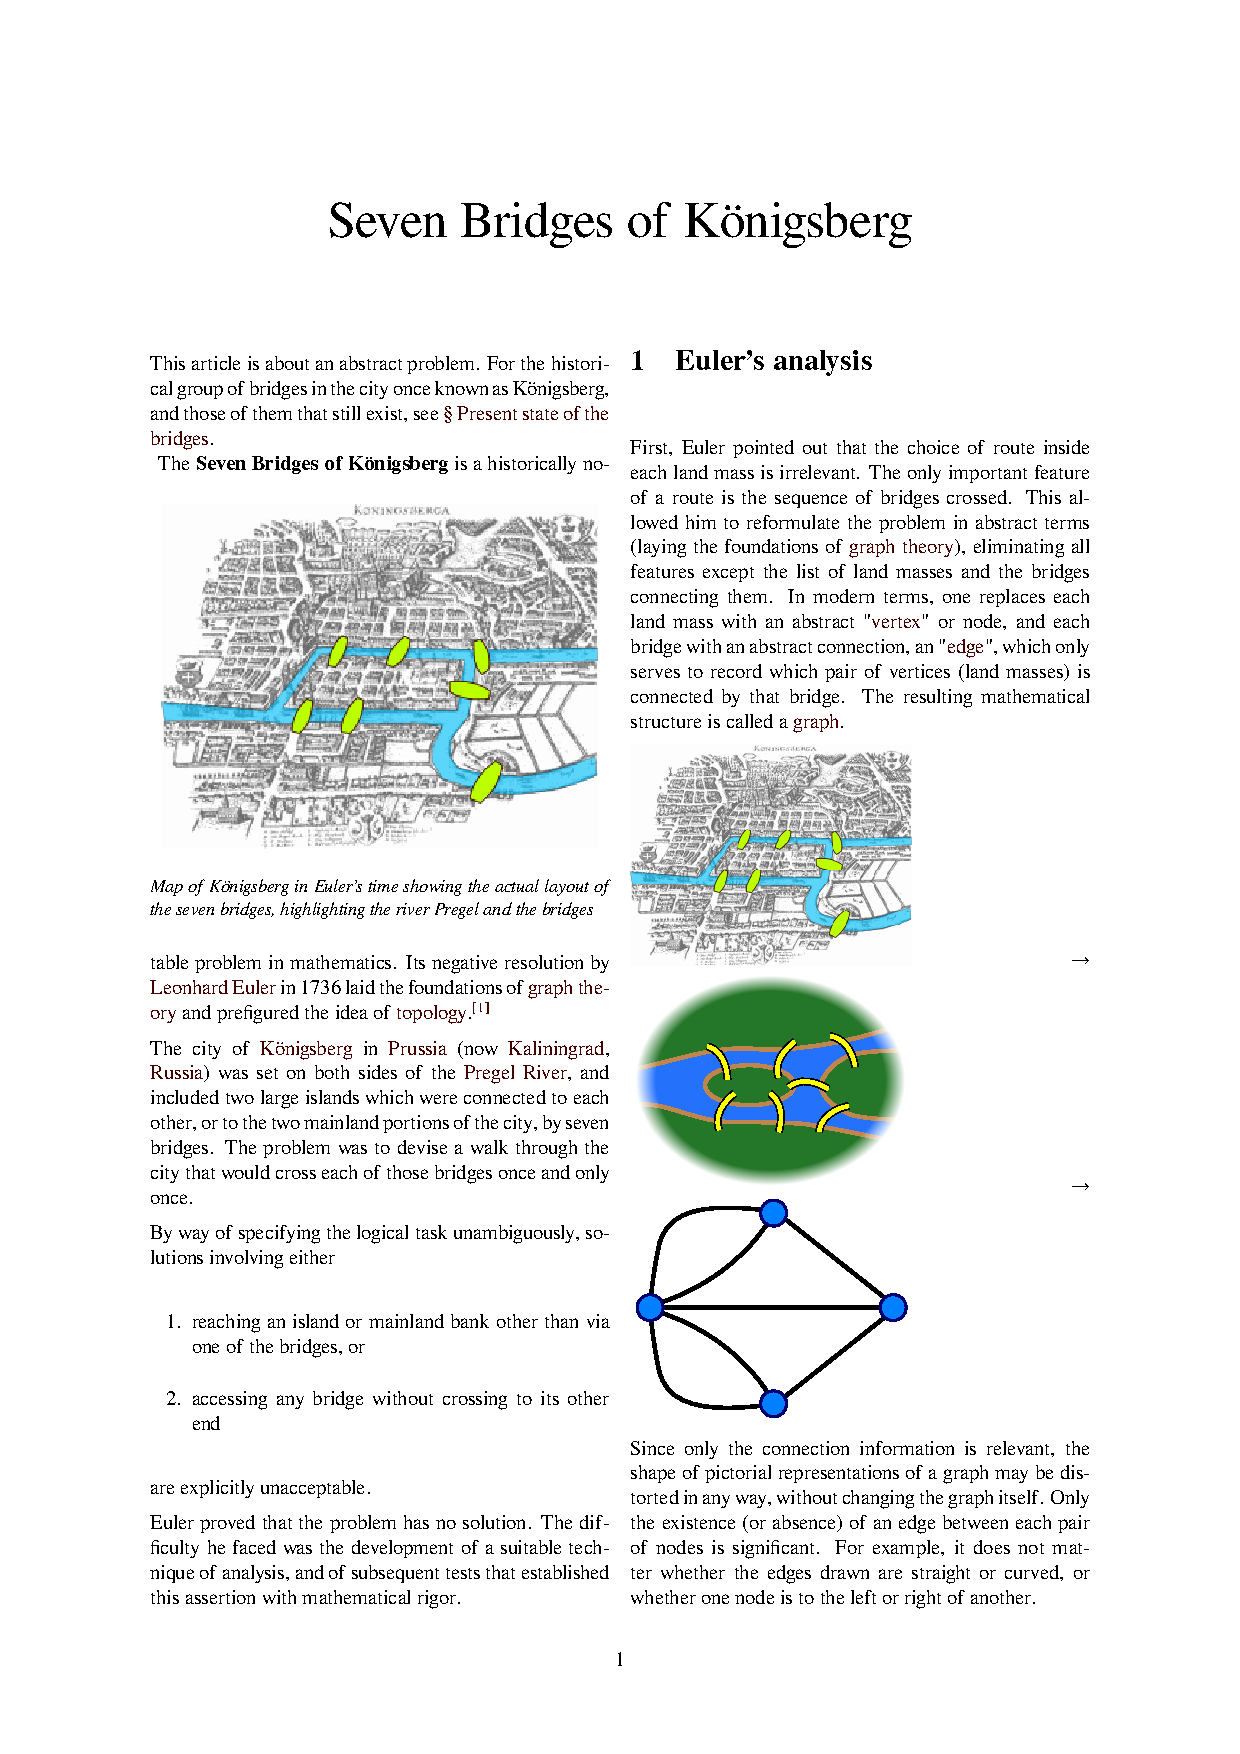
\includepdf[pages=-,offset= 0 0]{Chapters/SBridgesofK.pdf}

\section{The First Theorem of Graph Theory}

For a vertex
$v$ in a graph  we denote the number of edges incident to $v$ as the {\bfseries {degree}}
of $v$, written as $deg(v)$. For example, consider the graph

\begin{center}
 \begin{tikzpicture}[node distance=1cm,
                               thick,main node/.style={circle,fill=blue!20,draw,outer sep=1pt}
                              ]        
             \node[main node] (1) at (0,0) {$u_5$};
             \node[main node] (2) at (1.5,1.5) {$u_1$};
             \node[main node] (3) at (3,0) {$u_2$};
             \node[main node] (4) at (2.5,-2.00) {$u_3$};
             \node[main node] (5) at (0.55,-2.00) {$u_4$};
             \node (G) at (1.50,-0.50) {$G$};          
             \path%
               (1) edge node [right] {} (2)  %{} is where the edge value would go
               (2) edge [right] node {} (3)
               (3) edge [right] node {} (4)
               (4) edge [left] node {} (5)
               (5) edge [left] node {} (1)
               (1) edge [left] node {} (4);
         \end{tikzpicture}
\end{center}

Vertices $u_1, u_2, u_4$ each have degree $2$, while $deg(u_3)$ and $deg(u_5)$ are each $3$.
The list of the degrees of the vertices of a graph is called the {\bfseries degree sequence} of the graph.
The degrees are traditionally listed in increasing order. So the degree sequence of the graph $G$ above is $2,2,2,3,3$.

The following theorem is usually referred to as the {\it First Theorem of Graph Theory}


\begin{thm}
 The sum of the degrees of the vertices of a graph equals twice the number of edges. In particular, the sum of the degrees is even.
\end{thm}
\begin{proof}
 Notice that, when adding the degrees for the vertices,
each edge will contribute two to the total, once for each end.
So the sum of the degrees is twice the number of edges. 
\end{proof}

For example, in the graph $G$ above, there are $6$ edges, and the sum of the degrees of the vertices is $2+2+2+3+3= 12 = 2(6)$.


\begin{corollary}
 A graph must have an even number of vertices of odd degree.
 \end{corollary}
 \begin{proof}
Split the vertices into two groups: the vertices with even degree and the vertices with odd degree. The sum of all the degrees is even, and the sum of all the even degrees is also even. That implies that the sum of all the odd degrees must also be even. Since an odd number of odd integers adds up to an odd integer, it must be that there is an even number of odd degrees.
\end{proof}

\section{A Brief Catalog of Special Graphs} 
 

It is convenient to have names for some particular types of graphs that occur frequently. 

For $n\geq 1$, $K_n$ denotes the graph with $n$ vertices where every pair of vertices
 is adjacent.  $K_n$ is the {\bfseries {complete graph}} on $n$ vertices. So $K_{n}$ is the largest possible graph with $n$ vertices in the sense that it has the maximum possible number of edges.
 \begin{marginfigure}
 \begin{tikzpicture}[node distance=3cm,
                        thick,main node/.style={circle,fill=blue!20,draw,outer sep=1pt}
                       ]    
      \node[main node] (1) at (0.000,1.000) {};
      \node[main node] (2) at (0.866,0.500) {};
      \node[main node] (3) at (0.866,-0.500) {};
      \node[main node] (4) at (0.00,-1.000) {};
      \node[main node] (5) at (-0.866,-0.500) {};
      \node[main node] (6) at (-0.866,0.500) {};      
       \node (K6) at (-0.866,-1.000) {$K_{6}$};    
      \path%
        (1) edge node [right] {} (2)  %{} is where the edge value would go
        (1) edge [right] node {} (3)
        (1) edge [right] node {} (4)
        (1) edge [left] node {} (5)
        (1) edge [left] node {} (6)
        (2) edge [left] node {} (3)
        (2) edge [left] node {} (4)
        (2) edge [right] node {} (5)
        (2) edge [right] node {} (6)
        (3) edge [right] node {} (4)
        (3) edge [left] node {} (5)
        (3) edge [left] node {} (6)
        (4) edge [left] node {} (5)
        (4) edge [left] node {} (6)
        (5) edge [right] node {} (6);
 \end{tikzpicture}
 \end{marginfigure}

 
  For $n\geq 3$, $C_n$ denotes the graph with $n$ vertices, $v_1,...,v_n$, where 
each vertex in that list is adjacent to the vertex that follows it and $v_n$ is adjacent to $v_1$. The graph  $C_n$ is called the {\bfseries {$n$-cycle}}. The graph $C_3$ is called a {\bfseries triangle}.
 
  \begin{marginfigure}
 \begin{tikzpicture}[node distance=3cm,
                        thick,main node/.style={circle,fill=blue!20,draw,outer sep=1pt}
                       ]    
      \node[main node] (1) at (0.000,1.000) {};
      \node[main node] (2) at (0.866,0.500) {};
      \node[main node] (3) at (0.866,-0.500) {};
      \node[main node] (4) at (0.00,-1.000) {};
      \node[main node] (5) at (-0.866,-0.500) {};
      \node[main node] (6) at (-0.866,0.500) {};      
       \node (C6) at (-0.866,-1.000) {$C_{6}$};    
      \path%
        (1) edge node [right] {} (2)  %{} is where the edge value would go        
        (2) edge [left] node {} (3)        
        (3) edge [right] node {} (4)        
        (4) edge [left] node {} (5)       
        (5) edge [right] node {} (6)
        (6) edge [left] node {} (1);
 \end{tikzpicture}
 \end{marginfigure}

 For $n\geq 2$, $L_n$ denotes the {\bfseries {$n$-link}}. An $n${-}link is a row of $n$ vertices with each vertex adjacent to the following vertex.
  Alternatively, for $n\geq 3$, an $n${-}link is produced by erasing one edge from an $n${-}cycle. 
  
  \begin{marginfigure}
 \begin{tikzpicture}[node distance=3cm,
                        thick,main node/.style={circle,fill=blue!20,draw,outer sep=1pt}
                       ]    
      \node[main node] (1) at (-2,-1.0) {};
      \node[main node] (2) at (-1,-1.0) {};
      \node[main node] (3) at (0,-1.0) {};
      \node[main node] (4) at (1,-1.0) {};
      \node[main node] (5) at (2,-1.0) {};
      \node[main node] (6) at (3,-1.0) {};      
       \node (L6) at (.5,-1.500) {$L_{6}$};    
      \path%
        (1) edge node [right] {} (2)  %{} is where the edge value would go        
        (2) edge [left] node {} (3)        
        (3) edge [right] node {} (4)        
        (4) edge [left] node {} (5)       
        (5) edge [right] node {} (6);       
 \end{tikzpicture}
 \end{marginfigure}

 For $n\geq 3$, $W_n$ denotes the {\bfseries {$n$-wheel}}. To form $W_n$ add one vertex
 to $C_n$ and make it adjacent to every other vertex. Notice that the $n$-wheel has $n+1$ vertices.
 
 \begin{marginfigure}
 \begin{tikzpicture}[node distance=3cm,
                        thick,main node/.style={circle,fill=blue!20,draw,outer sep=1pt}
                       ]    
      \node[main node] (1) at (0.000,1.000) {};
      \node[main node] (2) at (0.866,0.500) {};
      \node[main node] (3) at (0.866,-0.500) {};
      \node[main node] (4) at (0.00,-1.000) {};
      \node[main node] (5) at (-0.866,-0.500) {};
      \node[main node] (6) at (-0.866,0.500) {};   
      \node[main node] (7)  at (0.00, 0.00) {};
       \node (W6) at (-0.866,-1.000) {$W_{6}$};    
      \path%
        (1) edge node [right] {} (2)  %{} is where the edge value would go        
        (2) edge [left] node {} (3)        
        (3) edge [right] node {} (4)        
        (4) edge [left] node {} (5)       
        (5) edge [right] node {} (6)
        (6) edge [left] node {} (1)
        (1) edge node [right] {} (7)         
        (2) edge [left] node {} (7)        
        (3) edge [right] node {} (7)        
        (4) edge [left] node {} (7)       
        (5) edge [right] node {} (7)
        (6) edge [left] node {} (7);

 \end{tikzpicture}
 \end{marginfigure}
 
  For $n\geq 1$, the {\bfseries {$n$-cube}}, $Q_n$, is the graph whose vertices are labeled with the $2^{n}$ bit  strings
 of length $n$. The unusual choice of names for the vertices is made so it will be easy to describe the edges in the graph: two vertices are adjacent provided their labels differ in exactly one bit. Except for $n = 1,2,3$ it is not easy to draw a convincing diagram of $Q_{n}$. The graph $Q_{3}$ can be drawn so it looks like what you would probably draw if you wanted a picture of a 3-dimensional cube. In the graph below, there is a vertex placed at each of the eight corners of the $3${-}cube labeled with the name of the vertex.
 
 \begin{center}
 \begin{tikzpicture}[thick,scale=3]
    \coordinate (A1) at (0, 0);
    \node at (0, -.1)  {$000$};
    \coordinate (A2) at (0, 1);
    \node at (1, -.1)  {$010$};
    \coordinate (A3) at (1, 1);
    \node at (1.5, .3)  {$110$};
    \coordinate (A4) at (1, 0);
     \node at (.5, .38)  {$100$};
    \coordinate (B1) at (0.3, 0.3);
    \node at (-.2,1 )  {$001$};
    \coordinate (B2) at (0.3, 1.3);
    \node at (.25, 1.38)  {$101$};
    \coordinate (B3) at (1.3, 1.3);
    \node at (1.5, 1.38)  {$111$};
    \coordinate (B4) at (1.3, 0.3);
     \node at (.8, 1.1)  {$011$};

    \draw (A1) -- (A2);
    \draw (A2) -- (A3);
    \draw (A3) -- (A4);
    \draw (A4) -- (A1);

    \draw (A1) -- (B1);
    \draw (B1) -- (B2);
    \draw (A2) -- (B2);
    \draw (B2) -- (B3);
    \draw (A3) -- (B3);
    \draw (A4) -- (B4);
    \draw (B4) -- (B3);
    \draw (B1) -- (B4);
    
\end{tikzpicture}    

\end{center}
 
  A graph is {\bfseries {bipartite}} if it is possible to split the vertices into two subsets, let's call them $T$ and $B$ for top and bottom, so that all the edges  go from a vertex in one of the subsets to a vertex in the other subset.
  
  For example, the graph below is a bipartite graph  with  $T = \{a,b,c\}$ and $B = \{d,e,f,g\}$. 
  
 \begin{center} 
  \begin{tikzpicture}[node distance=1cm,
                      thick,main node/.style={circle,fill=blue!20,draw,outer sep=1pt,
                      inner sep=2pt,minimum size=15pt}
                     ]           
   \node[main node] (a) at (0.0,0.0) {$a$};
   \node[main node] (b) at (3.0,0.0) {$b$};
   \node[main node] (c) at (6.0,0.0) {$c$};
   \node[main node] (d) at (0.0,-3.0) {$d$};
   \node[main node] (e) at (3.0,-3.0) {$e$};       
   \node[main node] (f) at (6.0,-3.0) {$f$};
   \node[main node] (g) at (9.0,-3.0) {$g$};
   \path%
     (a) edge node [right] {} (d)  %{} is where the edge value would go
     (a) edge [left] node {} (e)    
     (a) edge [left] node {} (f)
     (b) edge [left] node {} (e)
     (b) edge [left] node {} (d)
     (c) edge [left] node {} (e)
     (c) edge [left] node {} (f)
     (c) edge [left] node {} (g);
\end{tikzpicture}
\end{center}
  
   
  
  

    
    If $T$  has $m$ vertices and $B$ has $n$ vertices, and every vertex in $T$ is adjacent to every vertex in $B$,  the graph  is called the {\bfseries {complete bipartite graph}}, and it is denoted by $K_{m,n}$. Here is the graph $K_{3,4}$:
    
     \begin{center} 
  \begin{tikzpicture}[node distance=1cm,
                      thick,main node/.style={circle,fill=blue!20,draw,outer sep=1pt,
                      inner sep=2pt,minimum size=15pt}
                     ]           
   \node[main node] (a) at (0.0,0.0) {$a$};
   \node[main node] (b) at (3.0,0.0) {$b$};
   \node[main node] (c) at (6.0,0.0) {$c$};
   \node[main node] (d) at (0.0,-3.0) {$d$};
   \node[main node] (e) at (3.0,-3.0) {$e$};       
   \node[main node] (f) at (6.0,-3.0) {$f$};
   \node[main node] (g) at (9.0,-3.0) {$g$};
   \node (K34) at (4.5,-3.5) {$K_{3,4}$}; 
   
   \path%
     (a) edge node [right] {} (d)  %{} is where the edge value would go
     (a) edge [left] node {} (e)    
     (a) edge [left] node {} (f)
     (a) edge [left] node {} (g)
     (b) edge node [right] {} (d) 
     (b) edge [left] node {} (e)    
     (b) edge [left] node {} (f)
     (b) edge [left] node {} (g)
     (c) edge node [right] {} (d)
     (c) edge [left] node {} (e)    
     (c) edge [left] node {} (f)
     (c) edge [left] node {} (g);
     
\end{tikzpicture}
\end{center}
  
It is not always obvious if a graph is bipartite or not when looking at a diagram. For example  the square 
\begin{center} 
  \begin{tikzpicture}[node distance=1cm,
                      thick,main node/.style={circle,fill=blue!20,draw,outer sep=1pt,
                      inner sep=2pt,minimum size=15pt}
                     ]           
   \node[main node] (a) at (0.0,0.0) {$a$};
   \node[main node] (b) at (3.0,0.0) {$b$};
   \node[main node] (c) at (3.0,3.0) {$c$};
   \node[main node] (d) at (0.0,3.0) {$d$};
   
   
   \path%
     (a) edge node [right] {} (b)  %{} is where the edge value would go
     (b) edge [left] node {} (c)    
     (c) edge [left] node {} (d)
     (d) edge [left] node {} (a);     
\end{tikzpicture}
\end{center}

is bipartite since the graph can be redrawn as

\begin{center} 
  \begin{tikzpicture}[node distance=1cm,
                      thick,main node/.style={circle,fill=blue!20,draw,outer sep=1pt,
                      inner sep=2pt,minimum size=15pt}
                     ]           
   \node[main node] (d) at (0.0,0.0) {$d$};
   \node[main node] (b) at (3.0,0.0) {$b$};
   \node[main node] (c) at (3.0,3.0) {$c$};
   \node[main node] (a) at (0.0,3.0) {$a$};
   
   
   \path%
     (a) edge node [right] {} (b)  %{} is where the edge value would go
     (b) edge [left] node {} (c)    
     (c) edge [left] node {} (d)
     (d) edge [left] node {} (a);     
\end{tikzpicture}
\end{center}

so we can see the graph is actually $K_{2,2}$ in disguise.




\section{Graph isomorphisms}

The graphs $G$ and $H$ are obviously really the same except for the labels used for the vertices.

\begin{center}
\begin{tikzpicture}[node distance=1cm,
                               thick,main node/.style={circle,fill=blue!20,draw,outer sep=1pt}]     
             \node[main node] (1) at (0,0) {$a$};
             \node[main node] (2) at (1.5,1.5) {$c$};
             \node[main node] (3) at (-1.5,1.5) {$b$};
             \node (G) at (-1,0) {$G$};          
             \path%
               (1) edge node [right] {} (2)  %{} is where the edge value would go
               (1) edge [right] node {} (3);
         \end{tikzpicture}
         \hskip 50pt
         \begin{tikzpicture}[node distance=1cm,
                                 thick,main node/.style={circle,fill=blue!20,draw,outer sep=1pt}]
             \node[main node] (1) at (0,0) {$x$};
             \node[main node] (2) at (1.5,1.5) {$z$};
             \node[main node] (3) at (-1.5,1.5) {$y$};
             \node (H) at (-1,0) {$H$};          
             \path%
               (1) edge node [right] {} (2)  %{} is where the edge value would go
               (1) edge [right] node {} (3);                       
           \end{tikzpicture}
\end{center}

This idea of {\it sameness} (the official phrase is  the graphs $G$ and $H$ are {\bfseries isomorphic}) for graphs is defined as follows: Two graphs $G$ and $H$ are isomorphic provided we can relabel the vertices of one of the graphs using the labels of the other graph in such a way that the two graphs will have exactly the same edges. As you can probably guess, the notion of isomorphic graphs is an equivalence relation on the collection of all graphs.

In the example above, if the vertices of $H$ are relabeled as $a\to x$ (meaning replace $x$ with $a$), and 
$b\to y$, $c\to z$, then the graph $H$ will have edges $\{a,b\}$ and $\{a,c\}$ just like the graph $G$. So we have proved $G$ and $H$ are isomorphic graphs. The set of  replacement rules, $a\to x$, $b\to y$, $c\to z$, is called
an {\bfseries isomorphism}.

The graph $G$ is also isomorphic to the $3$-link $L_{3}$: 
\begin{center}
\begin{tikzpicture}[node distance=1cm,
                               thick,main node/.style={circle,fill=blue!20,draw,outer sep=1pt}]     
             \node[main node] (1) at (0,0) {$s$};
             \node[main node] (2) at (-1.5,0) {$r$};
             \node[main node] (3) at (1.5,0) {$t$};
             \node (L3) at (0,-.75) {$L_{3}$};          
             \path%
               (1) edge node [right] {} (2)  %{} is where the edge value would go
               (1) edge [right] node {} (3);
         \end{tikzpicture}
\end{center}    

In this case, an isomorphism is $a\to s$, $b\to r$, $c\to t$. 

On the other hand, $G$ is certainly not isomorphic to the $4$-cycle, $C_{4}$ since that graph does not even have the same number of vertices as $G$. Also $G$ is not isomorphic to the $3$-cycles, $C_{3}$. In this case, the two graphs do have the same number of vertices, but not the same number of edges.  For two graphs have a chance of being isomorphic, the two graphs must have the same number of vertices and the same number of edges. 
 But {\bfseries warning}: even if two graphs have the same number of vertices and the same number of edges, they need not be isomorphic.  For example $L_4$ and $K_{1,3}$ are both graphs with $4$ vertices and $3$ edges, but 
they are not isomorphic. This is so since $L_{4}$ does not have a vertex of degree $3$, but $K_{1,3}$ does.

 Extending that idea: to have a chance of being isomorphic, two graphs will have to have the same degree sequences since they will end up with the same edges after relabeling. But even having the same degree sequences is not enough to conclude two graphs are isomorphic as the margin example shows. We can see those two graphs are not isomorphic since $G$ has three vertices that form a triangle, but there are no triangles in $H$.

%\figure~\ref{fig:G  not cong H}.
\begin{marginfigure}
 \begin{tikzpicture}[node distance=3cm,
                        thick,main node/.style={circle,fill=blue!20,draw,outer sep=1pt}
                       ]    
      \node[main node] (1) at (0.000,1.000) {};
      \node[main node] (2) at (0.866,0.500) {};
      \node[main node] (3) at (0.866,-0.500) {};
      \node[main node] (4) at (0.00,-1.000) {};
      \node[main node] (5) at (-0.866,-0.500) {};
      \node[main node] (6) at (-0.866,0.500) {};      
       \node (G) at (-0.866,-1.000) {$G$};    
      \path%
        (1) edge node [right] {} (2)  %{} is where the edge value would go
        (2) edge [right] node {} (3)
        (3) edge [right] node {} (4)
        (4) edge [left] node {} (5)
        (5) edge [left] node {} (6)
        (6) edge [left] node {} (1)
        (2) edge [left] node {} (6)
        (3) edge [right] node {} (5);
 \end{tikzpicture}
 \qquad
 \begin{tikzpicture}[node distance=3cm,
                        thick,main node/.style={circle,fill=blue!20,draw,outer sep=1pt}
                       ]
      \node[main node] (1) at (0.000,1.000) {};
      \node[main node] (2) at (0.866,0.500) {};
      \node[main node] (3) at (0.866,-0.500) {};
      \node[main node] (4) at (0.00,-1.000) {};
      \node[main node] (5) at (-0.866,-0.500) {};
      \node[main node] (6) at (-0.866,0.500) {};      
      \node (G) at (-0.866,-1.000) {$H$};    
      \path%
        (1) edge node [right] {} (2)  %{} is where the edge value would go
        (2) edge [right] node {} (3)
        (3) edge [right] node {} (4)
        (4) edge [left] node {} (5)
        (5) edge [left] node {} (6)
        (6) edge [left] node {} (1)
        (2) edge [left] node {} (5)
        (3) edge [right] node {} (6);
 \end{tikzpicture}
\caption{Nonisomorphic grades with the same degree sequences.}
\end{marginfigure}

\vskip 30pt
For graphs with a few vertices and a few edges, a little trial and error is typically enough to determine if the graphs are isomorphic. For more complicated graphs, it can be very difficult to determine if they are isomorphic or not.  One of the big goals in theoretical computer science is the design of  efficient algorithms to determine if two graphs are isomorphic.    

\begin{exmp}
   \begin{marginfigure}
        \begin{tikzpicture}[node distance=1cm,
                               thick,main node/.style={circle,fill=blue!20,draw,outer sep=1pt}
                              ]        
             \node[main node] (1) at (0,0) {$e$};
             \node[main node] (2) at (1.5,1.5) {$a$};
             \node[main node] (3) at (3,0) {$b$};
             \node[main node] (4) at (2.5,-2.00) {$c$};
             \node[main node] (5) at (0.55,-2.00) {$d$};
             \node (G) at (1.50,-0.50) {$G$};          
             \path%
               (1) edge node [right] {} (2)  %{} is where the edge value would go
               (2) edge [right] node {} (3)
               (3) edge [right] node {} (4)
               (4) edge [left] node {} (5)
               (5) edge [left] node {} (1);
         \end{tikzpicture}
         \begin{tikzpicture}[node distance=1cm,
                                 thick,main node/.style={circle,fill=blue!20,draw,outer sep=1pt}
                                ]           
               \node[main node] (1) at (0,0) {$z$};
               \node[main node] (2) at (1.5,1.5) {$v$};
               \node[main node] (3) at (3,0) {$w$};
               \node[main node] (4) at (2.5,-2.00) {$x$};
               \node[main node] (5) at (0.55,-2.00) {$y$};       
               \node (H) at (1.50,-0.50) {$H$};
               \path%
                 (1) edge node [right] {} (3)  %{} is where the edge value would go
                 (3) edge [right] node {} (5)
                 (5) edge [right] node {} (2)
                 (2) edge [left] node {} (4)
                 (4) edge [left] node {} (1);
           \end{tikzpicture}
           \caption{Isomorphic graphs}\label{fig:iso graphs}
      \end{marginfigure}%
  Let $G$ be a 5-cycle on $a,b,c,d,e$ drawn as a regular pentagon
  with vertices
  arranged clockwise, in order, at the corners. Let $H$ have vertex set $v,w,x,y,z$ and graphical 
  presentation as a pentagram (five-pointed star), where the vertices of the graph are the ends of the 
  points of the star, and are arranged clockwise, (see figure~\ref{fig:iso graphs}). \\
  An isomorphism is $a\to v, \; b\to x,\;  c\to z,\;  d\to w,\; e\to y.$ 
\end{exmp}

\vfill\break


\begin{exmp}\label{petersen graph}
 The two graphs in figure~\ref{fig:more iso graphs} are isomorphic as shown by using the relabeling 
 \[
  u_1 \to v_1,\; u_2\to v_2,\; u_3\to v_3,\;
   u_4\to v_4, \; u_5\to v_9,
 \]  
 \[  
    u_6\to v_{10},\; u_7\to  v_5,\; 
   u_8\to v_7,\; u_9\to  v_8,\; u_{10}\to v_6.
 \]
 \begin{figure}
 \resizebox{\textwidth}{!}{%
 \centering
   \begin{tikzpicture}[node distance=2cm,
                       thick,main node/.style={circle,fill=blue!20,draw,outer sep=1pt,inner sep=1pt,minimum size=20pt}
                               ]        
              \node[main node] (2) at (0,4) {$u_2$};
              \node[main node] (3) at (3.804,1.236) {$u_3$};
              \node[main node] (4) at (2.352,-3.236) {$u_4$};
              \node[main node] (5) at (-2.352,-3.236) {$u_5$};
              \node[main node] (1) at (-3.804,1.236) {$u_1$};
              \node[main node] (9) at (0,2) {$u_9$};
              \node[main node] (8) at (1.902,0.618) {$u_8$};
              \node[main node] (7) at (1.176,-1.618) {$u_7$};
              \node[main node] (6) at (-1.176,-1.618) {$u_6$};
              \node[main node] (10) at (-1.902,0.618) {$u_{10}$}; 
              \node (G) at (-3.804,4.625) {$G$};        
              \path%
                (1) edge node [right] {} (2)  %{} is where the edge value would go
                (2) edge [right] node {} (3)
                (3) edge [right] node {} (4)
                (4) edge [left] node {} (5)
                (5) edge [left] node {} (1)
                (1) edge [left] node {} (10)
                (2) edge [left] node {} (9)
                (3) edge [left] node {} (8)
                (4) edge [left] node {} (7)
                (5) edge [left] node {} (6)
                (6) edge [left] node {} (8)
                (8) edge [left] node {} (10)
                (10) edge [left] node {} (7)
                (7) edge [left] node {} (9)
                (9) edge [left] node {} (6);                              
          \end{tikzpicture}
         \qquad
          \begin{tikzpicture}[node distance=3cm,
                              thick,main node/.style={circle,fill=blue!20,draw,outer sep=1pt,inner sep=1pt,minimum size=20pt}
                                 ]
                \node[main node] (2) at (0.000,4.000) {$v_2$};
                \node[main node] (3) at (3.464,2.000) {$v_3$};
                \node[main node] (4) at (3.464,-2.000) {$v_4$};
                \node[main node] (5) at (0.00,-4.000) {$v_5$};
                \node[main node] (6) at (-3.464,-2.000) {$v_6$};
                \node[main node] (1) at (-3.464,2.000) {$v_1$};
                \node[main node] (7) at (-1.732,-1.000) {$v_7$};
                \node[main node] (8) at (0.000,2.000) {$v_8$};
                \node[main node] (9) at (1.732,-1.000) {$v_9$};
                \node[main node] (10) at (0.000,0.000) {$v_{10}$};   
                 \node (H) at (-3.464,4.000) {$H$};
                \path%
                  (1) edge node [right] {} (2)  %{} is where the edge value would go
                  (2) edge [right] node {} (3)
                  (3) edge [right] node {} (4)
                  (4) edge [left] node {} (5)
                  (5) edge [left] node {} (6)
                  (6) edge [left] node {} (1)
                  (2) edge [right] node {} (8)
                  (4) edge [right] node {} (9)
                  (6) edge [right] node {} (7)
                  (7) edge [right] node {} (10)
                  (8) edge [right] node {} (10)
                  (9) edge [right] node {} (10)
                  (1) edge [bend right] node {} (9)
                  (3) edge [bend right] node {} (7)
                  (5) edge [bend right] node {} (8);
           \end{tikzpicture}%
        } %end resizebox
    \caption{More Isomorphic graphs}\label{fig:more iso graphs}
 \end{figure}
\end{exmp}
The graph $G$ is the traditional presentation of the {\bfseries {Petersen Graph}}.
It could be described as the graph whose vertex set is labeled with  all the two element subsets of a five element set, with an edge
joining two vertices if their labels have exactly one element in common. 

\section{Paths}\label{sect:paths}

The origins of graph theory had to do with bridges, and possible routes crossing the bridges. In this section we will consider that sort of question in graphs in general. We will think of walking along edges, from one vertex in the list to the next, and visiting vertices. Remember that we do not allow multiple edges or loops in our graphs. 

We begin with a collection of definitions. Warning: These terms are used differently in different texts. If you look at another graph theory text, be sure to see how the terms are used there.

A {\bfseries path} of {\bfseries {length}} $n$ in a graph is a sequence of $n+1$ vertices
$v_0, v_1, v_2,..., v_n$, where each vertex in the list is adjacent to the following vertex. Repeated vertices and repeated edges in a path are allowed.  The vertices $v_0$ and $v_{n}$ are the {\bfseries endpoints} of the path. Think of starting at $v_0$, walking along the edges, and ending up at $v_n$. The length $n$ of the walk is the number of edges transversed in the path.    A path of length three or more for which the endpoints are the same (so $v_0 = v_n$) is called a {\bfseries circuit}. A {\bfseries simple} path (or circuit) is one that does not repeat any edges. A single vertex $v$ will be considered to be a path (but not a circuit!) of length $0$.



Here is an example illustrating these definitions.

\begin{exmp}
 In the graph shown in figure~\ref{fig:paths in a graph}, 
 $a,b,e,c,f,c$ is a path of length $5$. 
 That is an example of an $a,c${-}path, meaning it starts at vertex $a$ and ends at vertex $c$. 
 That path is not simple since the edge ${c,f}$ is repeated. Note that direction does not matter. 
 The vertex sequence $a,b,c,f,e$ is an $a,e${-}path.  Here are two simple circuits in that graph: $a,b,e,d,a$ and $a,b,c,e,d,a$. Notice that the circuit $a,e,b,c,f,e,d,a$ is also simple even though it repeats the vertex $e$. It does not repeat any edges.  
 
\begin{marginfigure}
\resizebox{\textwidth}{!}{%
 \begin{tikzpicture}[node distance=1cm,
                      thick,main node/.style={circle,fill=blue!20,draw,outer sep=1pt,
                      inner sep=2pt,minimum size=15pt}
                     ]           
   \node[main node] (a) at (0.0,0.0) {$a$};
   \node[main node] (b) at (3.0,0.0) {$b$};
   \node[main node] (c) at (6.0,0.0) {$c$};
   \node[main node] (d) at (0.0,-3.0) {$d$};
   \node[main node] (e) at (3.0,-3.0) {$e$};       
   \node[main node] (f) at (6.0,-3.0) {$f$};
   \path%
     (a) edge node [right] {} (b)  %{} is where the edge value would go
     (b) edge [right] node {} (c)
     (c) edge [right] node {} (f)
     (f) edge [left] node {} (e)
     (e) edge [left] node {} (d)
     (d) edge [left] node {} (a)
     (a) edge [left] node {} (e)
     (b) edge [left] node {} (e)
     (c) edge [left] node {} (e);
\end{tikzpicture}
} %end resizebox
\caption{paths and circuits}\label{fig:paths in a graph}
\end{marginfigure}
\end{exmp} 

A graph is {\bfseries {connected}} if there is a path between any two vertices. In plain English, a connected graph consists of a single piece. The individual connected pieces of a graph are called its {\bfseries connected components}. The length of the shortest path between two vertices in a connect component of a graph is called the {\bfseries distance} between the vertices.  In  figure~\ref{fig:paths in a graph},
the distance between $a$ and $f$ is $2$. 

\begin{thm}\label{thm:exists simple path}
 In a connected graph there is a simple path between
 any two vertices. In other words, if there is a way to get from one vertex to another vertex along edges, then there
 is a way to get between those two vertices without repeating any edges.
\end{thm}
\begin{proof}
Problem~\ref{prob:prove thm simple path}. The idea is simple: in a path with a repeated edge, just eliminate the {\it side trip} made between the two occurrences of that edge from the path. Do that until all the repeated edges are eliminated. For example,  in the graph shown in figure~\ref{fig:paths in a graph}, The $a,c${-}path $a,e,b,e,c$ can be reduced to the path $a,e,c$, eliminating the side trip to $b$.
\end{proof}


A vertex in a graph is a {\bfseries {cut vertex}}, if removal of the vertex and edges incident to it 
results in a graph with more connected components. Similarly a {\bfseries {bridge}} is an edge whose removal (keeping the vertices it is incident to) 
yields a graph with more connected components.

We close this section with a discussion of two special types of paths.

\subsection{Eulerian paths and circuits}

An {\bfseries {eulerian path}} in a graph is a simple path which transverses every edge of the graph. In other words, an eulerian path in a graph is a path that transverses every edge of the graph exactly once. 
An interesting property 
of a graph with an eulerian path is that it can be drawn completely
without lifting pencil from paper and without retracing any edges.

An {\bfseries {eulerian circuit}} is a simple circuit in a graph that transverses every edge of the graph. So an eulerian circuit  is a path of length three or more that transverses every edge of the graph and ends up at its initial vertex.
A graph is called {\bfseries eulerian} if it has an eulerian circuit.

\begin{exmp}
 The graph $C_5$ is an eulerian graph. In fact, the graph itself is an eulerian circuit. 
\end{exmp}


\begin{exmp}
 The graph $K_5$ is an eulerian graph. 
\end{exmp}

\begin{exmp}
 The graph $L_n$ is itself an eulerian path, but does not have an eulerian circuit.
\end{exmp}

\begin{exmp}
 The graph $K_4$ is not an eulerian graph. \sidenote{Try it!}.
\end{exmp}

\subsection{Hamiltonian paths and circuits}

A {\bfseries {hamiltonian path}} in a graph is a simple path that visits every vertex in the graph exactly once.
A {\bfseries {hamiltonian circuit}} in a graph is a simple circuit that, except for the last vertex of the circuit, visits every vertex in the graph exactly once.
A graph is {\bfseries hamiltonian} if it has a hamiltonian circuit.

\begin{exmp}
 $K_n$ is hamiltonian for $n\geq 3$.
\end{exmp} 

\begin{exmp}
 $W_n$ has a hamiltonian circuit for $n\geq 3$.
\end{exmp} 

\begin{exmp}
 $L_n$ has no hamiltonian circuit for $n\geq 2$
\end{exmp} 

\subsection{Some facts about eulerian and hamiltonian graphs}

A few easy observation: if $G$ is a graph with either an eulerian circuit  or hamiltonian
circuit, then
\begin{enumerate}
 \item $G$ is connected.
 
 \item every vertex has degree at least 2.
 
 \item $G$ has no bridges.
 
 \end{enumerate}
 
 If $G$ has a hamiltonian circuit, then $G$ has no cut vertices. 

Leonhard Euler gave a simple way to determine exactly when a graph is eulerian. On the other hand,  despite considerable effort, no one has been able to devise a test to distinguish between hamiltonian and nonhamiltonian graphs that is much better than a brute force trial{-}and{-}error search for a hamiltonian circuit. 

\begin{thm}
 A connected graph is eulerian if and only if  every vertex has even degree.
\end{thm}
\begin{proof}
 Let $G$ be an eulerian graph, and suppose that $v$ is a vertex in 
 $G$ with odd degree, say $2m+1$. Let $i$ denote the number of times an eulerian circuit  passes through 
 $v$. Since every edge is used exactly once in the circuit, and each time $v$ is visited two different edges are used, 
 we have $2i=2m+1$, which is impossible. $\ctrdct$. So $G$ cannot have any vertices of odd degree.
 
 Conversely, let $G$ be a connected graph where every vertex has even degree. 
 Select a vertex $u$ and build  a simple path starting at $u$ as long as possible:
 each time we visit a vertex we select an unused edge leaving that vertex to extend the simple path. For any vertex $v\neq u$ we visit,  its even
 degree guarantees there will be an unused edge out, since each time $v$ is visited used two edges incident to $v$ and one more edge to arrive at $v$, for a total of an odd number of edges incident to $v$, and the vertex has even degree, so there must be at least one unused edge leading out of $v$.
 Since the process of extending the simple path must eventually come to an end, that shows the end must be at $u$ when the simple path cannot be extended, and so we have constructed an eulerian circuit. 
  
 If this simple path contains every edge we are done. Otherwise when these edges are removed from $G$
 we obtain a set of connected components $H_1,...,H_m$ which are subgraphs of $G$ and which
 each satisfy that all vertices have even degree. Since their sizes are smaller, we may inductively
 construct an eulerian circuit for each $H_i$. Since each $G$ is connected, each $H_i$ contains
 a vertex of the initial circuit, say $v_j$. If we call the eulerian circuit of $H_i$, $C_i$, then 
 $v_0,...v_j,C_i,v_j,...,v_n,v_0$ is a circuit in $G$. Since the $H_i$ are disjoint, we may insert each 
 eulerian {\it partial} circuit thus obtaining an eulerian circuit for $G$.
\end{proof} 

As a corollary we have
\begin{thm}
 A connected graph has an eulerian path, but not an eulerian circuit,   if
 and only if
 it has exactly two vertices of odd degree.
\end{thm}

The following theorem is an example of a sufficient (but not necessary) condition for a graph to have a hamiltonian
circuit. 
\begin{thm}
 Let $G$ be a connected graph with $n\geq 3$ vertices. If $deg(v)\geq n/2$
 for every vertex $v$, then $G$ is hamiltonian.
\end{thm}
\begin{proof}
 Suppose that the theorem is false.
 Let $G$ be a connected graph with $deg(v)\geq n/2$
 for every vertex $v$.
 Moreover suppose that of all counterexamples on $n$ vertices, $G$ is a graph with the largest possible number of edges. 
 
 $G$ is not complete, since $K_n$ has a hamiltonian circuit, for $n\geq 3$. Therefore
 $G$ has two nonadjacent vertices $v_1$ and $v_n$. By maximality
 the graph $G_1$ formed by adding the edge $\{v_1,v_n\}$ to $G$ has a hamiltonian circuit. Moreover this circuit uses the
 edge $\{v_1,v_n\}$, since otherwise $G$ has a hamiltonian circuit. So we may suppose that the hamiltonian
 circuit in $G_1$ is of the form $v_1,v_2,...,v_n,v_1$. Thus $v_1,...,v_n$ is a  path
 in $G$.
 
 Let $k=deg(v_1)$. 
 If $v_{i+1}$ is adjacent to $v_1$, then $v_i$ cannot be adjacent to $v_n$, since otherwise $v_1,...,v_i,v_n,v_{n-1},...,v_{i+1},v_1$ is a
 hamiltonian circuit in $G$. Therefore, we have the contradiction
 \[
  deg(v_n)\leq (n-1)-k\leq n-1-n/2=n/2-1.\ctrdct
 \]
\end{proof} 

{\bfseries WARNING}:  Do not read too much into this theorem. The condition is  not a necessary condition. The $5${-}cycle, $C_5$, is obviously hamiltonian, but the vertices all have degree $2$ which is less than $\frac{5}{2}$.

\bigskip

\section{Trees}
Trees form an important class of graphs. A {\bfseries {tree}} is a connected graph with
no circuits.  Trees are traditionally drawn {\it upside down}, with the tree growing down rather than up,  starting at a root vertex.
 
\begin{center}
\begin{tikzpicture}[level distance=1.5cm,
  level 1/.style={sibling distance=4cm},
  level 2/.style={sibling distance=1.5cm}]
  \node {root}
    child {node {left}
      child {node {lleft}}
      child {node {rleft}}
    }
    child {node {right}
      child {node {lright}}
      child {node {midright}}
      child {node {rright}}
   };
\end{tikzpicture}
\end{center}

\begin{thm}\label{thm:graph is tree}
 A graph $G$ is a tree if and only if there is a unique path between any two vertices.
\end{thm}
\begin{proof}
 Suppose that $G$ is a tree, and let $u$ and $v$ be two vertices of $G$. Since
 $G$ is connected, there is a path of the form $u=v_0,v_1,...,v_n=v$. 
 If there is a different  path from $u$ to $v$, say $u=w_0,w_1,...,w_n=v$ let $i$ be the smallest subscript
 so that $w_i=v_i$, but $v_{i+1}\neq w_{i+1}$. Also let $j$ be the next smallest subscript where $v_j=w_j$.
 By construction $v_i,v_{i+1},...,v_j,w_{j-1},w_{j-2},...,w_i$ is a circuit in $G \ctrdct$.
 
 Conversely, if $G$ is a graph where there is a unique path between any pair of vertices, then
 by definition $G$ is connected. If $G$ contained a circuit, $C$, then any two vertices of $C$ would be joined
 by two distinct paths.$\ctrdct$ Therefore $G$ contains no circuits, and is a tree.
\end{proof}

A consequence of theorem~\ref{thm:graph is tree} is that given any vertex $r$ in a tree, 
we can draw the tree with $r$ at the
top, as the root vertex,  and the other vertices in levels below. \sidenote {Redraw the tree diagram above with vertex midright as the root vertex.} The neighbors of $r$ that appear at the first level below $r$
are called $r$'s {\bfseries {children}}. The children of $r$'s children are put
in the second level below $r$, and are $r$'s {\bfseries {grandchildren}}. In general the $i$th level consists of those
vertices in the tree which are at distance $i$ from $r$. The result is called a {\bfseries {rooted tree}}. The {\bfseries {height}} of a rooted tree is the maximum level number.

Naturally, besides child and parent, many genealogical terms apply to rooted trees,
and are suggestive of the structure. For example if  a rooted tree
has root $r$, and $v\not{=}r$, the {\bfseries {ancestors}} of $v$ are all vertices on the 
path from $r$ to $v$, including $r$, but excluding $v$. The {\bfseries {descendants}} of a vertex, $w$
consist of all vertices which have $w$ as one of their ancestors. The {\bfseries {subtree rooted at $w$}}
is the rooted tree consisting of $w$, its descendants, and all the required edges. 
A vertex with no children is a {\bfseries {leaf}}, and a vertex with at least one child is called an
{\bfseries {internal vertex}}.

To distinguish rooted trees by breadth, we use the term {\bfseries {$m$-ary}} to mean that any internal
vertex has at most $m$ children. An $m$-ary tree is {\bfseries {full}} if every internal vertex has
exactly $m$ children. When $m=2$, we use the term {\bfseries {binary}}.


\begin{thm}
 A tree on $n$ vertices has $n-1$ edges.
\end{thm}
\begin{proof}
 ({\it by induction on n.})\\
\underbar{Basis}: Let $n = 1$, this is the trivial tree with $0$ edges.  So true the theorem is true for $n = 1$.

\underbar{Inductive Step}:
Suppose that for some $n\geq 1$ every tree with $n$ vertices has $n-1$ edges.
Now suppose $T$ is a tree with $n+1$ vertices. Let $v$ be a leaf of $T$.
If we erase $v$ and the edge leading to it, we are left with a tree with $n$ vertices.
By the inductive hypothesis, this new tree will have $n-1$ edges. Since it has one less edge than the original tree, we conclude $T$ has $n$ edges.
\end{proof}

\clearpage
\section{Exercises}

\begin{exer}
Find a graph isomorphism $\phi: G \to H$. Verify the adjacency preserving property 
by showing the adjacency matrices satisfy $A_G = A_G^\phi$.

\vspace*{2\baselineskip}
\begin{minipage}[b]{0.4\textwidth}
($G$)\quad\linebreak\begin{tikzpicture}[node distance=0.5cm,
                       thick,main node/.style={circle,fill=blue!20,draw,outer sep=2pt,inner sep=2pt}
                      ] 
  \node[main node] (a) at (-2.00,1.00) {$a$};
  \node[main node] (b) at (2.00,1.00) {$b$};
  \node[main node] (c) at (2.00,-1.00) {$c$};
  \node[main node] (d) at (-2.00,-1.00) {$d$};
  \node[main node] (e) at (0.00,-0.50) {$e$};
  \node[main node] (f) at (1.00,0.00) {$f$};
  \node[main node] (g) at (0.00,0.50) {$g$};
  \node[main node] (h) at (-1.00,0.00) {$h$};

  \path%
   (a) edge [left] node {} (b)
   (a) edge [left] node {} (h)
   (a) edge [left] node {} (d)
   (b) edge [left] node {} (c)
   (b) edge [left] node {} (g)
   (c) edge [left] node {} (d)
   (c) edge [left] node {}  (f)
   (d) edge [left] node {} (e)
   (e) edge [left] node {} (f)
   (e) edge [left] node {} (h)
   (g) edge [left] node {} (h)
   (f) edge [left] node {} (g);
 \end{tikzpicture}
\end{minipage}
\hspace*{0.1\textwidth}
\begin{minipage}[b]{0.4\textwidth}
($H$)\quad\linebreak\begin{tikzpicture}[node distance=0.5cm,
                       thick,main node/.style={circle,fill=blue!20,draw,outer sep=2pt,inner sep=2pt}
                      ] 
  \node[main node] (s) at (-2.00,1.00) {$s$};
  \node[main node] (t) at (2.00,1.00) {$t$};
  \node[main node] (u) at (2.00,-1.00) {$u$};
  \node[main node] (v) at (-2.00,-1.00) {$v$};
  \node[main node] (w) at (-1.00,-0.50) {$w$};
  \node[main node] (x) at (1.00,-0.50) {$x$};
  \node[main node] (y) at (1.00,0.50) {$y$};
  \node[main node] (z) at (-1.00,0.50) {$z$};

  \path%
   (s) edge [left] node {} (t)
   (t) edge [left] node {} (u)
   (u) edge [left] node {} (v)
   (v) edge [left] node {} (s)
   (s) edge [left] node {} (w)
   (t) edge [left] node {} (x)
   (u) edge [left] node {} (y)
   (v) edge [left] node {} (z)
   (z) edge [left] node {} (y)
   (y) edge [left] node {} (x)
   (x) edge [left] node {} (w)
   (w) edge [left] node {} (z);
 \end{tikzpicture}
 \end{minipage}
\end{exer}

\begin{exer}
Prove that $G$ and  $H$ are not isomorphic.

\vspace*{2\baselineskip}
\begin{minipage}[b]{0.4\textwidth}
($G$)\quad\linebreak\begin{tikzpicture}[node distance=0.5cm,
                       thick,main node/.style={circle,fill=blue!20,draw,outer sep=2pt,inner sep=2pt}
                      ] 
  \node[main node] (a) at (-1.00,2.00) {$a$};
  \node[main node] (b) at (1.00,2.00) {$b$};
  \node[main node] (c) at (2.00,1.00) {$c$};
  \node[main node] (d) at (2.00,-1.00) {$d$};
  \node[main node] (e) at (1.00,-2.00) {$e$};
  \node[main node] (f) at (-1.00,-2.00) {$f$};
  \node[main node] (g) at (-2.00,-1.00) {$g$};
  \node[main node] (h) at (-2.00,1.00) {$h$};

  \path%
   (a) edge [left] node {} (b)
   (b) edge [left] node {} (c)
   (c) edge [left] node {} (d)
   (d) edge [left] node {} (e)
   (e) edge [left] node {} (f)
   (f) edge [left] node {} (g)
   (g) edge [left] node {} (h)
   (h) edge [left] node {} (a)
   (a) edge [left] node {} (c)
   (a) edge [left] node {} (e)
   (a) edge [left] node {} (g)
   (b) edge [left] node {} (d)
   (b) edge [left] node {} (f)
   (b) edge [left] node {} (h)
   (c) edge [left] node {} (e)
   (c) edge [left] node {} (g)   
   (d) edge [left] node {} (f)
   (d) edge [left] node {} (h)   
   (e) edge [left] node {} (g)
   (f) edge [left] node {} (h);
 \end{tikzpicture}
\end{minipage}
\hspace*{0.1\textwidth}
\begin{minipage}[b]{0.4\textwidth}
($H$)\quad\linebreak\begin{tikzpicture}[node distance=0.5cm,
                       thick,main node/.style={circle,fill=blue!20,draw,outer sep=2pt,inner sep=2pt}
                      ] 
  \node[main node] (s) at (-1.00,2.00) {$s$};
  \node[main node] (t) at (1.00,2.00) {$t$};
  \node[main node] (u) at (2.00,1.00) {$u$};
  \node[main node] (v) at (2.00,-1.00) {$v$};
  \node[main node] (w) at (1.00,-2.00) {$w$};
  \node[main node] (x) at (-1.00,-2.00) {$x$};
  \node[main node] (y) at (-2.00,-1.00) {$y$};
  \node[main node] (z) at (-2.00,1.00) {$z$};

  \path%
   (s) edge [left] node {} (t)
   (t) edge [left] node {} (u)
   (u) edge [left] node {} (v)
   (v) edge [left] node {} (w)
   (w) edge [left] node {} (x)
   (x) edge [left] node {} (y)
   (y) edge [left] node {} (z)
   (z) edge [left] node {} (s)
   (s) edge [left] node {} (v)
   (s) edge [left] node {} (w)
   (s) edge [left] node {} (x)
   (t) edge [left] node {} (w)
   (t) edge [left] node {} (x)
   (t) edge [left] node {} (y)
   (u) edge [left] node {} (x)
   (u) edge [left] node {} (y)
   (u) edge [left] node {} (z)
   (v) edge [left] node {} (y)
   (v) edge [left] node {} (z)
   (w) edge [left] node {} (z);
   
  \end{tikzpicture}
 \end{minipage}
\end{exer}

\begin{exer}
Redraw the graph $G$ as a bipartite graph.

\vspace*{2\baselineskip}
($G$)\quad\linebreak\begin{tikzpicture}[node distance=0.5cm,
                       thick,main node/.style={circle,fill=blue!20,draw,outer sep=2pt,inner sep=2pt}
                      ] 
  \node[main node] (1) at (-3.00,2.00) {$1$};
  \node[main node] (2) at (-1.00,2.00) {$2$};
  \node[main node] (3) at (1.00,2.00) {$3$};
  \node[main node] (4) at (3.00,2.00) {$4$};
  \node[main node] (5) at (3.00,0.00) {$5$};
  \node[main node] (6) at (1.00,0.00) {$6$};
  \node[main node] (7) at (-1.00,0.00) {$7$};
  \node[main node] (8) at (-3.00,0.00) {$8$};

  \path%
   (1) edge [left] node {} (2)
   (3) edge [left] node {} (4)
   (1) edge [left] node {} (8)
   (2) edge [left] node {} (7)
   (3) edge [left] node {} (6)
   (4) edge [left] node {} (5)
   (8) edge [left] node {} (7)
   (7) edge [left] node {} (6)
   (6) edge [left] node {} (5);
 \end{tikzpicture}
\end{exer}

\begin{exer}
Explain why the graph $G$ is not eulerian, but is hamiltonian.
\vspace*{2\baselineskip}
($G$)\quad\linebreak\begin{tikzpicture}[node distance=0.5cm,
                       thick,main node/.style={circle,fill=blue!20,draw,outer sep=2pt,inner sep=2pt}
                      ] 
  \node[main node] (a) at (-4.00,2.00) {$a$};
  \node[main node] (b) at (-2.00,2.00) {$b$};
  \node[main node] (c) at (-2.00,3.50) {$c$};
  \node[main node] (d) at (0.00,2.00) {$d$}; 
  \node[main node] (e) at (2.00,3.50) {$e$};
  \node[main node] (f) at (2.00,2.00) {$f$};
  \node[main node] (g) at (4.00,2.00) {$g$};
  \node[main node] (h) at (2.00,0.00) {$h$};
  \node[main node] (i) at (0.00,0.00) {$i$};
  \node[main node] (j) at (-2.00,0.00) {$j$};

  \path%
   (a) edge [left] node {} (b)
   (b) edge [left] node {} (c)
   (c) edge [left] node {} (d)
   (d) edge [left] node {} (e)
   (e) edge [left] node {} (f)
   (f) edge [left] node {} (g)
   (g) edge [left] node {} (h)
   (h) edge [left] node {} (i)
   (i) edge [left] node {}  (j)
   (j) edge [left] node {} (a)
   (i) edge [left] node {} (b)
   (i) edge [left] node {} (d)
   (i) edge [left] node {} (f);
 \end{tikzpicture}
\end{exer}

\begin{exer}
Find an eulerian circuit for the graph $G$ as a list of vertices.

\vspace*{2\baselineskip}

($G$)\quad\linebreak\begin{tikzpicture}[node distance=0.5cm,
                       thick,main node/.style={circle,fill=blue!20,draw,outer sep=2pt,inner sep=2pt}
                      ] 
  \node[main node] (a) at (-1.00,2.00) {$a$};
  \node[main node] (b) at (1.00,2.00) {$b$};
  \node[main node] (c) at (2.00,1.00) {$c$};
  \node[main node] (d) at (2.00,-1.00) {$d$};
  \node[main node] (e) at (1.00,-2.00) {$e$};
  \node[main node] (f) at (-1.00,-2.00) {$f$};
  \node[main node] (g) at (-2.00,-1.00) {$g$};
  \node[main node] (h) at (-2.00,1.00) {$h$};

  \path%
   (a) edge [left] node {} (b)
   (b) edge [left] node {} (c)
   (c) edge [left] node {} (d)
   (d) edge [left] node {} (e)
   (e) edge [left] node {} (f)
   (f) edge [left] node {} (g)
   (g) edge [left] node {} (h)
   (h) edge [left] node {} (a)
   (a) edge [left] node {} (d)
   (a) edge [left] node {} (f)
   (b) edge [left] node {} (e)
   (b) edge [left] node {} (g)
   (c) edge [left] node {} (f)
   (c) edge [left] node {} (h)   
   (d) edge [left] node {} (g)
   (d) edge [left] node {} (a)   
   (e) edge [left] node {} (h);
 \end{tikzpicture}
\end{exer}

\begin{exer}
Prove that the graph $G$ has no hamiltonian circuit.

\vspace*{2\baselineskip}
($G$)\quad\linebreak\begin{tikzpicture}[node distance=0.5cm,
                       thick,main node/.style={circle,fill=blue!20,draw,outer sep=2pt,inner sep=2pt}
                      ] 
  \node[main node] (a) at (-2.00,4.00) {$a$};
  \node[main node] (b) at (-1.00,3.00) {$b$};
  \node[main node] (c) at (0.00,4.00) {$c$};
  \node[main node] (d) at (2.0,4.00) {$d$};
  \node[main node] (e) at (1.00,3.00) {$e$};
  \node[main node] (f) at (1.00,1.00) {$f$};
  \node[main node] (g) at (2.0,0.00) {$g$};
  \node[main node] (h) at (0.00,0.00) {$h$};
  \node[main node] (i) at (-1.00,1.00) {$i$};
  \node[main node] (j) at (-2.00,0.00) {$j$};

  \path%
   (a) edge [left] node {} (b)
   (b) edge [left] node {} (c)
   (c) edge [left] node {} (d)
   (d) edge [left] node {} (g)
   (g) edge [left] node {} (h)
   (h) edge [left] node {} (j)
   (j) edge [left] node {} (a)
   (d) edge [left] node {} (e)
   (h) edge [left] node {} (f)
   (h) edge [left] node {} (i)
   (j) edge [left] node {} (i)
   (b) edge [left] node {} (e)
   (e) edge [left] node {} (f)
   (f) edge [left] node {} (i)
   (i) edge [left] node {} (b);
 \end{tikzpicture}
\end{exer}


\clearpage
\section{Problems}

\begin{prob}
\
 \begin{enumerate}[label = (\alph*)]
\item How many edges are there in $K_n$, the complete graph with $n$ vertices?
\item How many edges are there in $C_n$, the $n${-}cycle with $n$ vertices?
\item How many edges are there in $L_n$, the $n${-}link with $n$ vertices?
\item How many edges are there in $W_n$, the $n${-}wheel with $n+1$ vertices?
\item How many edges are there in $Q_n$, the $n${-}cube with $2^n$  vertices?
\item How many edges are there in $K_{m,n}$, the complete bipartite graph with $m$ {\itshape top} and $n$ {\itshape bottom} vertices?
\end{enumerate}
\end{prob}

\begin{prob}\label{prob:bipartite graphs}
Determine whether each graph is bipartite. If it is, redraw it as a bipartite graph.

\vspace*{\baselineskip}
\begin{minipage}[b]{0.4\textwidth}
(a)\quad\linebreak\begin{tikzpicture}[node distance=0.5cm,
                       thick,main node/.style={circle,fill=blue!20,draw,outer sep=2pt,inner sep=2pt}
                      ] 
  \node[main node] (a) at (-1.5,0) {$a$};
  \node[main node] (b) at (-0.75,1.00) {$b$};
  \node[main node] (c) at (0.75,1.00) {$c$};
  \node[main node] (d) at (1.5,0) {$d$};
  \node[main node] (e) at (0,-1.00) {$e$};
  \path%
   (a) edge [left] node {} (b)
   (a) edge [left] node {} (d)
   (a) edge [left] node {} (e)
   (b) edge [left] node {} (c)
   (b) edge [left] node {} (e)
   (c) edge [left] node {} (d)
   (c) edge [left] node {} (e);
 \end{tikzpicture}
\end{minipage}
\hspace*{0.1\textwidth}
\begin{minipage}[b]{0.4\textwidth}
 (b)\quad\linebreak\begin{tikzpicture}[node distance=1cm,
                     thick,main node/.style={circle,fill=blue!20,draw,outer sep=2pt,inner sep=1pt}
                    ]        
   \node[main node] (u1) at (0,0) {$u_1$};
   \node[main node] (u2) at (1,0.75) {$u_2$};
   \node[main node] (u3) at (2.0,0) {$u_3$};
   \node[main node] (u5) at (1.75,-1.25) {$u_5$};
   \node[main node] (u4) at (0.05,-1.25) {$u_4$};
   \node[main node] (u6) at (4.00,-1.25) {$u_6$};       
   \path%
     (u1) edge node [right] {} (u2)  %{} is where the edge value would go
     (u2) edge [right] node {} (u3)
     (u3) edge [right] node {} (u4)
     (u4) edge [left] node {} (u1)
     (u1) edge [left] node {} (u6)
     (u4) edge [left] node {} (u5)
     (u5) edge [left] node {} (u6)
     (u3) edge [left] node {} (u6);
 \end{tikzpicture}
\end{minipage}

\vspace*{\baselineskip}
\begin{minipage}[b]{0.4\textwidth}
(c)\quad\linebreak\begin{tikzpicture}[node distance=3cm,
                    thick,main node/.style={circle,fill=blue!20,draw,outer sep=2pt,inner sep=1pt}
                   ]  
  \node[main node] (v1) at (0.000,1.000) {$v_1$};
  \node[main node] (v6) at (0.866,0.500) {$v_6$};
  \node[main node] (v5) at (0.866,-0.500) {$v_5$};
  \node[main node] (v4) at (0.00,-1.000) {$v_4$};
  \node[main node] (v3) at (-0.866,-0.500) {$v_3$};
  \node[main node] (v2) at (-0.866,0.500) {$v_2$};          
  \path%
    (v1) edge node [right] {} (v2)  %{} is where the edge value would go
    (v2) edge [right] node {} (v3)
    (v3) edge [right] node {} (v4)
    (v4) edge [left] node {} (v5)
    (v5) edge [left] node {} (v6)
    (v6) edge [left] node {} (v1)
    (v3) edge [right] node {} (v6);
\end{tikzpicture}
\end{minipage}
\hspace*{0.1\textwidth}
\begin{minipage}[b]{0.4\textwidth}
 (d)\quad\linebreak\begin{tikzpicture}[node distance=3cm,
                     thick,main node/.style={circle,fill=blue!20,draw,outer sep=2pt,inner sep=1pt,minimum size=15pt}
                    ]  
   \node[main node] (b) at (0.000,1.000) {$b$};
   \node[main node] (c) at (0.866,0.500) {$c$};
   \node[main node] (d) at (0.866,-0.500) {$d$};
   \node[main node] (e) at (0.00,-1.000) {$e$};
   \node[main node] (f) at (-0.866,-0.500) {$f$};
   \node[main node] (a) at (-0.866,0.500) {$a$};          
   \path%
     (b) edge node [right] {} (a)  %{} is where the edge value would go
     (a) edge [right] node {} (f)
     (f) edge [right] node {} (e)
     (e) edge [left] node {} (d)
     (d) edge [left] node {} (c)
     (c) edge [left] node {} (b)
     (f) edge [right] node {} (c)
     (b) edge [right] node {} (e);
 \end{tikzpicture}
\end{minipage}

\end{prob}


\begin{prob}
\ 
 \begin{enumerate}[label = (\alph*)]
 \item For which values of $n$ is $C_n$ bipartite?\\[-3pt]
 \item For which values of $n$ is $Q_n$ bipartite?
\end{enumerate}
\end{prob}

\vfill\break

\begin{prob}
Draw the Petersen graph with vertices labeled with the ten different subsets of the five element set $\{a,b,c,d,e\}$ as suggested in example\ref{petersen graph}.
\end{prob}

\begin{prob}
 For the graph below
 \begin{enumerate}
  \item  Determine all the bridges.
  \item  Determine all the cut vertices.
 \end{enumerate}
 
 
\begin{tikzpicture}[thick,
                       main node/.style={circle,fill=blue!20,draw,outer sep=1pt,
                                         inner sep=1pt,minimum size=15pt}
                      ] 
   \node[main node] (a) at (0.0,3.0) {$a$};
   \node[main node] (b) at (2.0,3.0) {$b$};
   \node[main node] (c) at (4.0,3.0) {$c$};
   \node[main node] (d) at (6.0,3.0) {$d$};
   \node[main node] (e) at (8.0,3.0) {$e$};
   \node[main node] (f) at (10.0,3.0) {$f$};
   \node[main node] (g) at (3.0,1.5) {$g$};
   \node[main node] (h) at (7.0,1.5) {$h$};
   
   \path%
    (a) edge [left] node {} (b)
    (b) edge [left] node {} (c)
    (d) edge [left] node {} (e)
    (e) edge [left] node {} (f)
    (b) edge [left] node {} (g)
    (c) edge [left] node {} (g)
    (d) edge [left] node {} (h)
    (g) edge [left] node {} (h)
    (e) edge [left] node {} (h);
  \end{tikzpicture}
\end{prob}  


\begin{prob} 
For each candidate degree sequence below, either draw a graph with that degree sequence or explain why that list cannot be the degree sequence of a graph.

\begin{enumerate}
\item $4,4,4,4,4$   
\item $6,4,4,4,4$   
\item $0,0,0,0,0$   
\item $3,2,1,1,1$   
\item $3,3,2,2,1$   
\end{enumerate}
\end{prob}

\vfill\break

\begin{prob}
 For each pair of graphs either prove that $G_1$ and $G_2$ are not isomorphic, or else show they are isomorphic by exhibiting a graph isomorphism.
 
\vspace*{\baselineskip}
\begin{minipage}[b]{0.5\textwidth}
(a)\quad\linebreak
 %   \includegraphics{./Graphics/exer38-3-a.pdf}
%% exer38-3-a
\begin{tikzpicture}[scale=.5,thick, outer sep=0pt,inner sep=1pt]
    \def \N {7}
    \def \radius {2}
    \foreach [count=\x] \k in {1,2,...,\N}
        \node[black, circle,fill=blue!20, draw] (p\x) at ({360/\N * (\k - 1)}:\radius) {$u_{\x}$};

    \draw \foreach \x [remember=\x as \lastx (initially 1)] in {3,5,7,2,4,6,1}{(p\lastx) -- (p\x)};
     \draw \foreach \x [remember=\x as \lastx (initially 1)] in {4,7,3,6,2,5,1}{(p\lastx) -- (p\x)};
\node (G1) at (0,-3.00) {$G_1$};     
\end{tikzpicture}
\quad
\begin{tikzpicture}[scale=.5,thick, outer sep=0pt,inner sep=1pt]
    \def \N {7}
    \def \radius {2}
    \foreach [count=\x] \k in {1,...,\N}
        \node[black, circle, fill=blue!20, draw] (p\x) at ({360/\N * (\k - 1)}:2) {$v_{\x}$};

    \draw \foreach \x [remember=\x as \lastx (initially 1)] in {4,7,3,6,2,5,1}{(p\lastx) -- (p\x)};
     \draw \foreach \x [remember=\x as \lastx (initially 1)] in {2,3,...,\N,1}{(p\lastx) -- (p\x)}; 
   \node (G2) at (0,-3.00) {$G_2$};
\end{tikzpicture} 
\end{minipage}
\hspace*{0.15\textwidth}
\begin{minipage}[b]{0.6\textwidth}
 (b)\quad\linebreak
%    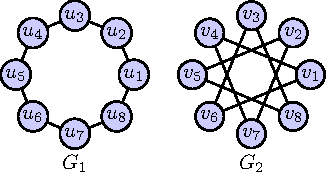
\includegraphics{./Graphics/exer38-3-b.pdf}
% exer38-3-b
\begin{tikzpicture}[scale=.5,thick, outer sep=0pt,inner sep=1pt]
    \foreach [count=\x] \k in {1,2,...,8}
        \node[black, circle,fill=blue!20, draw] (p\x) at ({360/8 * (\k - 1)}:2) {$u_{\x}$};

    \draw \foreach \x [remember=\x as \lastx (initially 1)] in {2,3,...,8,1}{(p\lastx) -- (p\x)};
    \node (G1) at (0,-3.00) {$G_1$};      
\end{tikzpicture}
\quad
\begin{tikzpicture}[scale=.5,thick, outer sep=0pt,inner sep=1pt]
    \foreach [count=\x] \k in {1,...,8}
        \node[black, circle, fill=blue!20, draw] (p\x) at ({360/8 * (\k - 1)}:2) {$v_{\x}$};

    \draw \foreach \x [remember=\x as \lastx (initially 1)] in {4,7,2,5,8,3,6,1}{(p\lastx) -- (p\x)};
    \node (G2) at (0,-3.00) {$G_2$};
\end{tikzpicture}
\end{minipage}

\vspace*{\baselineskip}
\begin{minipage}[b]{0.5\textwidth}
(c)\quad\linebreak
%   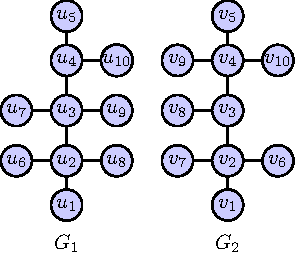
\includegraphics{./Graphics/exer38-3-c.pdf}
%% exer38-3-c
\begin{tikzpicture}[scale=.5,thick, outer sep=0pt,inner sep=0pt,minimum size=15pt]
    \node[black, circle,fill=blue!20, draw] (u1) at (0,-3.2) {$u_1$};
    \node[black, circle,fill=blue!20, draw] (u2) at (0,-1.7) {$u_2$};
    \node[black, circle,fill=blue!20, draw] (u3) at (0,0)  {$u_3$};
    \node[black, circle,fill=blue!20, draw] (u4) at (0,1.7)  {$u_4$};
    \node[black, circle,fill=blue!20, draw] (u5) at (0,3.2)  {$u_5$};
    \node[black, circle,fill=blue!20, draw] (u6) at (-1.7,-1.7) {$u_6$};
    \node[black, circle,fill=blue!20, draw] (u7) at (-1.7,0)  {$u_7$};
    \node[black, circle,fill=blue!20, draw] (u8) at (1.7,-1.7)  {$u_8$};
    \node[black, circle,fill=blue!20, draw] (u9) at (1.7,0)   {$u_9$};
    \node[black, circle,fill=blue!20, draw] (u10) at (1.7,1.7)  {$u_{10}$};
    \path%
      (u1) edge [left] node {} (u2)
      (u2) edge [left] node {} (u3)
      (u3) edge [left] node {} (u4)
      (u4) edge [left] node {} (u5)
      (u2) edge [left] node {} (u6)
      (u2) edge [left] node {} (u8)
      (u3) edge [left] node {} (u7)
      (u3) edge [left] node {} (u9)
      (u4) edge [left] node {} (u10);
   \node (G1) at (0,-4.5) {$G_1$};
\end{tikzpicture}
\quad
\begin{tikzpicture}[scale=.5,thick, outer sep=0pt,inner sep=0pt,minimum size=15pt]
    \node[black, circle,fill=blue!20, draw] (v1) at (0,-3.2) {$v_1$};
    \node[black, circle,fill=blue!20, draw] (v2) at (0,-1.7) {$v_2$};
    \node[black, circle,fill=blue!20, draw] (v3) at (0,0)  {$v_3$};
    \node[black, circle,fill=blue!20, draw] (v4) at (0,1.7)  {$v_4$};
    \node[black, circle,fill=blue!20, draw] (v5) at (0,3.2)  {$v_5$};
    \node[black, circle,fill=blue!20, draw] (v7) at (-1.7,-1.7) {$v_7$};
    \node[black, circle,fill=blue!20, draw] (v8) at (-1.7,0)  {$v_8$};
    \node[black, circle,fill=blue!20, draw] (v6) at (1.7,-1.7)  {$v_6$};
    \node[black, circle,fill=blue!20, draw] (v10) at (1.7,1.7)   {$v_{10}$};
    \node[black, circle,fill=blue!20, draw] (v9) at (-1.7,1.7)  {$v_{9}$};
    \path%
      (v1) edge [left] node {} (v2)
      (v2) edge [left] node {} (v3)
      (v3) edge [left] node {} (v4)
      (v4) edge [left] node {} (v5)
      (v2) edge [left] node {} (v6)
      (v3) edge [left] node {} (v8)
      (v2) edge [left] node {} (v7)
      (v4) edge [left] node {} (v9)
      (v4) edge [left] node {} (v10);
   \node (G2) at (0,-4.5) {$G_2$};
\end{tikzpicture}
\end{minipage}
\hspace*{0.15\textwidth}
\begin{minipage}[b]{0.6\textwidth}
 (d)\quad\linebreak
%    \includegraphics{./Graphics/exer38-3-d.pdf}
\begin{tikzpicture}[scale=.5,thick, outer sep=0pt,inner sep=0pt,minimum size=15pt]
    \node[black, circle,fill=blue!20, draw] (u1) at (0,3.2) {$u_1$};
    \node[black, circle,fill=blue!20, draw] (u2) at (1.7,1.7) {$u_2$};
    \node[black, circle,fill=blue!20, draw] (u3) at (1.7,-1.7)  {$u_3$};
    \node[black, circle,fill=blue!20, draw] (u4) at (0,-3.2)  {$u_4$};
    \node[black, circle,fill=blue!20, draw] (u5) at (-1.7,-1.7)  {$u_5$};
    \node[black, circle,fill=blue!20, draw] (u6) at (-1.7,1.7) {$u_6$};
    \path%
      (u1) edge [left] node {} (u2)
      (u2) edge [left] node {} (u3)
      (u3) edge [left] node {} (u4)
      (u4) edge [left] node {} (u5)
      (u5) edge [left] node {} (u6)
      (u6) edge [left] node {} (u1)
      (u1) edge [left] node {} (u4)
      (u2) edge [left] node {} (u6)
      (u2) edge [left] node {} (u5)
      (u3) edge [left] node {} (u5);
   \node (G1) at (0,-4.5) {$G_1$};
\end{tikzpicture}
\quad
\begin{tikzpicture}[scale=.5,thick, outer sep=0pt,inner sep=0pt,minimum size=15pt]
    \node[black, circle,fill=blue!20, draw] (v1) at (-1.7,3.2) {$v_1$};
    \node[black, circle,fill=blue!20, draw] (v2) at (1.7,3.2) {$v_2$};
    \node[black, circle,fill=blue!20, draw] (v3) at (1.7,-3.2)  {$v_3$};
    \node[black, circle,fill=blue!20, draw] (v4) at (-1.7,-3.2)  {$v_4$};
    \node[black, circle,fill=blue!20, draw] (v5) at (0,1.7)  {$v_5$};
    \node[black, circle,fill=blue!20, draw] (v6) at (0,-1.7)  {$v_6$};
    \path%
      (v1) edge [left] node {} (v2)
      (v2) edge [left] node {} (v3)
      (v3) edge [left] node {} (v4)
      (v4) edge [left] node {} (v1)
      (v1) edge [left] node {} (v5)
      (v2) edge [left] node {} (v5)
      (v3) edge [left] node {} (v6)
      (v4) edge [left] node {} (v6)
      (v5) edge [left] node {} (v6)
      (v1) edge [right] node {} (v3);
   \node (G2) at (0,-4.5) {$G_2$};
\end{tikzpicture}
\end{minipage}
\end{prob}


\begin{prob}\label{prob:prove thm simple path}
 Prove theorem~\ref{thm:exists simple path} from section~\ref{sect:paths}
 on paths:
 \emph{If $G$ is a connected graph, then there is a simple path between
  any two different vertices.}
\end{prob}

\vfill\break

\begin{prob}
 For each graph below
 \begin{enumerate*}[label=(\roman*)]
  \item  find an eulerian circuit, or prove that none exists, and 
  \item  find a hamiltonian circuit or prove that none exists.
 \end{enumerate*}
  
\begin{enumerate}[label=(\alph*),itemsep=0.5cm]
  \item The $3$-cube $Q_3$.
 
 \item
 \ \linebreak
 \begin{minipage}{0.5\textwidth}
  \begin{tikzpicture}[thick,main node/.style={circle,fill=blue!20,draw,outer sep=1pt,inner sep=1pt,minimum size=15pt}
                      ]  
   \node[main node] (a) at (0,1.5) {$a$};
   \node[main node] (b) at (1.5,1.5) {$b$};
   \node[main node] (c) at (3.0,1.5) {$c$};
   \node[main node] (d) at (4.5,1.5) {$d$};
   \node[main node] (i) at (0,0) {$i$};
   \node[main node] (h) at (1.5,0) {$h$};
   \node[main node] (g) at (3.0,0) {$g$};
   \node[main node] (f) at (4.5,0) {$f$};
   \node[main node] (e) at (6.0,0) {$e$};
   \path%
    (a) edge [left] node {} (b)
    (a) edge [bend left] node  {} (c)
    (a) edge [left] node {} (i)
    (b) edge [left] node {} (c)
    (b) edge [left] node {} (h)
    (b) edge [left] node {} (i)
    (c) edge [left] node {} (d)
    (c) edge [left] node {} (f)
    (c) edge [left] node {} (g)
    (c) edge [left] node {} (i)
    (d) edge [left] node {} (f)
    (d) edge [left] node {} (g)
    (d) edge [left] node {} (h)
    (e) edge [left] node {} (f)
    (e) edge [bend left] node {} (g)
    (f) edge [bend left] node {} (h)
    (g) edge [left] node {} (h)
    (h) edge [left] node {} (i);
  \end{tikzpicture}
 \end{minipage}
 %\clearpage
 \item
 \ \linebreak
 \begin{minipage}{0.5\textwidth}
  \begin{tikzpicture}[thick,
                       main node/.style={circle,fill=blue!20,draw,outer sep=1pt,
                                         inner sep=1pt,minimum size=15pt}
                      ] 
   \node[main node] (a) at (0.0,3.0) {$a$};
   \node[main node] (b) at (2.0,3.0) {$b$};
   \node[main node] (c) at (4.0,3.0) {$c$};
   \node[main node] (d) at (0.0,1.5) {$d$};
   \node[main node] (e) at (2.0,1.5) {$e$};
   \node[main node] (f) at (4.0,1.5) {$f$};
   \node[main node] (g) at (0.0,0.0) {$g$};
   \node[main node] (h) at (2.0,0.0) {$h$};
   \node[main node] (i) at (4.0,0.0) {$i$};
   \path%
    (a) edge [left] node {} (b)
    (a) edge [left] node {} (d)
    (b) edge [left] node {} (c)
    (b) edge [left] node {} (e)
    (b) edge [left] node {} (d)
    (c) edge [left] node {} (f)
    (d) edge [left] node {} (e)
    (d) edge [left] node {} (g)
    (e) edge [left] node {} (f)
    (e) edge [left] node {} (h)
    (f) edge [left] node {} (h)
    (f) edge [left] node {} (i)
    (g) edge [left] node {} (h)
    (h) edge [left] node {} (i);
  \end{tikzpicture}
 \end{minipage}
 
  \item The Petersen Graph. (See figure~\ref{fig:more iso graphs}.)

\end{enumerate}

\end{prob}

\begin{prob}
A {\it forest} is a graph consisting of one or more (separate) trees. If the total number of vertices in a forest is $f$, and the number of trees in the forest is $t$, what is the total number of edges in the forest?
\end{prob}

\begin{prob}
A tree is called {\bf star{-}like} if there is exactly one vertex with degree greater than $2$. How many different (that it, nonisomorphic) star{-}like trees are there with six vertices? (Note: If you draw the graph with the vertex of of degree greater than $2$ having the {\it arms} of the tree radiating out from it like spokes on a wheel, the name star{-}like will make sense.)
\end{prob}

\vfill\break

\begin{prob}\label{prob: rooted tree}
 Answer the following questions about the rooted tree shown in figure~\ref{fig:prob rooted tree}. 
 %(on page~\pageref{fig:prob rooted tree}.)
 
 \vspace*{0.25cm}
 \begin{minipage}{0.55\textwidth}
  \begin{enumerate}[label=(\alph*)]
    \item Which vertex is the root?
    \item Which vertices are internal?
    \item Which vertices are leaves?
    \item Which vertices are children of $b$?
    \item Which vertices are grandchildren of $b$?
  \end{enumerate}
  \end{minipage}
  \quad
 \begin{minipage}{0.55\textwidth}
  \begin{enumerate}[label=(\alph*)]\setcounter{enumi}{5}
    \item Which vertex is the parent of $m$?
    \item Which vertices are siblings of $q$?
    \item Which vertices are ancestors of $p$? 
    \item  Which vertices are descendants of $d$?
    \item  What level is $i$ at?
  \end{enumerate}  
 \end{minipage}

 \begin{figure}
  \centering
  \begin{tikzpicture}[thick]
   \node (root) at (0,0) {$a$};
   \node (l) at (-2.00,-1) {$b$};
   \node (ll) at (-3.00,-2) {$d$};
   \node (llm) at (-3.00,-3) {$i$};
   \node (llml) at (-3.50,-4) {$n$};
   \node (llmr) at (-2.50,-4) {$o$};
   \node (lm) at (-2.00,-2) {$e$};
   \node (lmm) at (-2.00,-3) {$j$};
   \node (lr) at (-1.00,-2) {$f$};
   \node (lrm) at (-1.00,-3) {$k$};
   \node (lrml) at (-1.50,-4) {$p$};
   \node (lrmr) at (-0.50, -4) {$q$};
   \node (r) at (2.00,-1) {$c$};
   \node (rl) at (1.00,-2) {$g$};
   \node (rlm) at (1.00,-3) {$l$};
   \node (rr) at (3.00,-2) {$h$};
   \node (rrm) at (3.00,-3) {$m$};
   \node (rrml) at (2.50,-4) {$r$};
   \node (rrmr) at (3.50,-4) {$s$};
   \path%
     (root) edge [left] node {} (l) %a to b
     (l) edge [left] node {} (ll) %b to d
     (ll) edge [left] node {} (llm) %d to i
     (llm) edge [left] node {} (llml) %i to n
     (llm) edge [left] node {} (llmr) %i to o
     (l) edge [left] node {} (lm) %b to e
     (lm) edge [left] node {} (lmm) %e to j
     (l) edge [left] node {} (lr) %b to f
     (lr) edge [left] node {} (lrm) %f to k
     (lrm) edge [left] node {} (lrml) %k to p
     (lrm) edge [left] node {} (lrmr) %k to q
     (root) edge [left] node {} (r) %root to c
     (r) edge [left] node {} (rl) %c to g
     (rl) edge [left] node {} (rlm) %g to l
     (r) edge [left] node {} (rr) %c to h
     (rr) edge [left] node {} (rrm) %h to m
     (rrm) edge [left] node {} (rrml) %m to r
     (rrm) edge [left] node {} (rrmr); %m to s
   \end{tikzpicture}%
  \caption{Tree for problem~\ref{prob: rooted tree}}\label{fig:prob rooted tree}
 \end{figure}
\end{prob}


 %Graphs



\appendix
\chapter{Answers to Exercises}
    \section*{Chapter 1}
\begin{Solution}{1.1}
\quad
    \begin{tasks}(1)
      \task yes
      \task no
      \task no
      \task This is not a proposition. As in many examples where a variable is involved,
this can be tricky. The truth value of this sentence depends on the value assigned to $x$. For example,
if $x$ is $2$, then $x=2$ is $T$ while $x^2-2x+1=0$ is $F$. So the entire sentence is $F$. On the
other hand, if $x$ is $0$, then both $x=2$ and $x^2-2x+1=0$ are $F$, so the sentence is $T$.
Since the sentence does not have a definite truth value, it is not a proposition. We'll have more
to say about this example in the next lesson.
      \task no (same reasoning as the previous item)
      \task* yes
    \end{tasks}%
  
\end{Solution}
\begin{Solution}{1.2}
\quad
   \begin{tasks}(2)
     \task
	\begin{tabular}{@{ }c@{ }@{ }c | c@{ }@{ }c@{ }@{ }c@{ }@{ }c@{ }@{ }c@{ }@{ }c}
	p & q &  & p & $\oplus$ & $\lnot$ & q & \\
	\hline
	T & T &  & T & \textcolor{red}{T} & F & T & \\
	T & F &  & T & \textcolor{red}{F} & T & F & \\
	F & T &  & F & \textcolor{red}{F} & F & T & \\
	F & F &  & F & \textcolor{red}{T} & T & F & \\
	\end{tabular}

      \task
         \begin{tabular}{@{ }c@{ }@{ }c | c@{ }@{}c@{}@{ }c@{ }@{ }c@{ }@{ }c@{ }@{}c@{ }}
              p & q & $\lnot$ & ( & q & $\rightarrow$ & p & )\\
              \hline
             T & T & \textcolor{red}{F} &  & T & T & T & \\
            T & F & \textcolor{red}{F} &  & F & T & T & \\
           F & T & \textcolor{red}{T} &  & T & F & F & \\
          F & F & \textcolor{red}{F} &  & F & T & F & \\
      \end{tabular}

    \task
       \begin{tabular}{@{ }c@{ }@{ }c | c@{ }@{ }c@{ }@{ }c@{ }@{ }c@{ }@{ }c@{ }@{ }c}
	p & q &  & q & $\land$ & $\lnot$ & p & \\
	\hline
	T & T &  & T & \textcolor{red}{F} & F & T & \\
	T & F &  & F & \textcolor{red}{F} & F & T & \\
	F & T &  & T & \textcolor{red}{T} & T & F & \\
	F & F &  & F & \textcolor{red}{F} & T & F & \\
    \end{tabular}

  \task
     \begin{tabular}{@{ }c@{ }@{ }c | c@{ }@{ }c@{ }@{ }c@{ }@{ }c@{ }@{ }c@{ }@{ }c}
	p & q &  & $\sim$ & q & $\lor$ & p & \\
	\hline
	T & T &  & F & T & \textcolor{red}{T} & T & \\
	T & F &  & T & F & \textcolor{red}{T} & T & \\
	F & T &  & F & T & \textcolor{red}{F} & F & \\
	F & F &  & T & F & \textcolor{red}{T} & F & \\
   \end{tabular}

  \task
      \begin{tabular}{@{ }c@{ }@{ }c@{ }@{ }c | c@{ }@{ }c@{ }@{ }c@{ }@{}c@{}@{ }c@{ }@{ }c@{ }@{ }c@{ }@{ }c@{ }@{}c@{}@{ }c}
	p & q & r &  & p & $\rightarrow$ & ( & $\lnot $ & q & $\land$ & r & ) & \\
	\hline
	T & T & T &  & T & \textcolor{red}{F} &  & F & T & F & T &  & \\
	T & T & F &  & T & \textcolor{red}{F} &  & F & T & F & F &  & \\
	T & F & T &  & T & \textcolor{red}{T} &  & T & F & T & T &  & \\
	T & F & F &  & T & \textcolor{red}{F} &  & T & F & F & F &  & \\
	F & T & T &  & F & \textcolor{red}{T} &  & F & T & F & T &  & \\
	F & T & F &  & F & \textcolor{red}{T} &  & F & T & F & F &  & \\
	F & F & T &  & F & \textcolor{red}{T} &  & T & F & T & T &  & \\
	F & F & F &  & F & \textcolor{red}{T} &  & T & F & F & F &  & \\
      \end{tabular}
   \end{tasks}
 
\end{Solution}
\begin{Solution}{1.3}
\quad\begin{fullwidth}
 \begin{enumerate}[label=\alph*),labelindent=0.25cm,leftmargin=*]
  \item $(1101\; 0111 \oplus 1110 \; 0010)\land 1100\; 1000=(0011\; 0101)\land 1100\; 1000=0000\; 0000$
  \item $(1111\; 1010\land 0111\; 0010)\lor (0101\; 0001)=(0111\; 0010)\lor (0101\; 0001)=0111\; 0011$
  \item $(1001\; 0010 \lor 0101\; 1101)\land (0110\;0010\lor 0111\; 0101)=(1101\; 1111)\land (0111\; 0111)=0101\;0111$
 \end{enumerate}
 \end{fullwidth}
\end{Solution}
\begin{Solution}{1.4}
\quad
    \begin{tasks}(3)
        \task $s \land \lnot f$
         \task $f \land \lnot s$
        \task $ \lnot s \to \lnot f$
    \end{tasks}
\end{Solution}
\begin{Solution}{1.5}
\quad
 \begin{enumerate}[label=\alph*),labelindent=0.25cm,leftmargin=*]
  \item Jordan did not play and the Wizards won.
  \item If Jordan played, then the Wizards lost.
  \item The Wizards won or Jordan played.
  \item Jordan didn't play when the Wizards won.
        OR If the   Wizards won, then Jordan did not play.
 \end{enumerate}
\end{Solution}
\begin{Solution}{1.6}
\quad
  \begin{tasks}(3)
       \task If Sam plays chess with the white pieces, he wins.
       \task  $(c\land \lnot w)\to b$
  \end{tasks}
\end{Solution}
 %Logical Connectives and Compound Propositions
    \section*{Chapter 2}
\begin{Solution}{2.1}
\quad
    \begin{tasks}(1)
        \task
\begin{tabular}{@{ }c@{ }@{ }c@{ }@{ }c | c@{ }@{}c@{}@{ }c@{ }@{ }c@{ }@{ }c@{ }@{}c@{}@{ }c@{ }@{ }c@{ }@{ }c | c@{ }@{ }c@{ }@{ }c@{ }@{}c@{}@{ }c@{ }@{ }c@{ }@{ }c@{ }@{}c@{}@{ }c}
p & q & r &  & ( & p & $\lor$ & q & ) & $\lor$ & r &  &  & p & $\lor$ & ( & q & $\lor$ & r & ) & \\
\hline
T & T & T &  &  & T & T & T &  & \textcolor{red}{T} & T &  &  & T & \textcolor{red}{T} &  & T & T & T &  & \\
T & T & F &  &  & T & T & T &  & \textcolor{red}{T} & F &  &  & T & \textcolor{red}{T} &  & T & T & F &  & \\
T & F & T &  &  & T & T & F &  & \textcolor{red}{T} & T &  &  & T & \textcolor{red}{T} &  & F & T & T &  & \\
T & F & F &  &  & T & T & F &  & \textcolor{red}{T} & F &  &  & T & \textcolor{red}{T} &  & F & F & F &  & \\
F & T & T &  &  & F & T & T &  & \textcolor{red}{T} & T &  &  & F & \textcolor{red}{T} &  & T & T & T &  & \\
F & T & F &  &  & F & T & T &  & \textcolor{red}{T} & F &  &  & F & \textcolor{red}{T} &  & T & T & F &  & \\
F & F & T &  &  & F & F & F &  & \textcolor{red}{T} & T &  &  & F & \textcolor{red}{T} &  & F & T & T &  & \\
F & F & F &  &  & F & F & F &  & \textcolor{red}{F} & F &  &  & F & \textcolor{red}{F} &  & F & F & F &  & \\
\end{tabular}

        \task
\begin{tabular}{@{ }c@{ }@{ }c | c@{ }@{ }c@{ }@{ }c@{ }@{ }c@{ }@{ }c | c@{ }@{ }c@{ }@{ }c@{ }@{ }c@{ }@{ }c@{ }@{ }c@{ }@{ }c}
p & q &  & p & $\rightarrow$ & q &  &  & $\lnot$ & q & $\rightarrow$ & $\lnot$ & p & \\
\hline
T & T &  & T & \textcolor{red}{T} & T &  &  & F & T & \textcolor{red}{T} & F & T & \\
T & F &  & T & \textcolor{red}{F} & F &  &  & T & F & \textcolor{red}{F} & F & T & \\
F & T &  & F & \textcolor{red}{T} & T &  &  & F & T & \textcolor{red}{T} & T & F & \\
F & F &  & F & \textcolor{red}{T} & F &  &  & T & F & \textcolor{red}{T} & T & F & \\
\end{tabular}

        \task
\begin{tabular}{@{ }c@{ }@{ }c | c@{ }@{ }c@{ }@{ }c@{ }@{ }c@{ }@{}c@{}@{ }c@{ }@{ }c@{ }@{ }c@{ }@{}c@{}@{ }c | c@{ }@{}c@{}@{ }c@{ }@{ }c@{ }@{ }c@{ }@{}c@{ }}
p & q &  & $\lnot$ & p & $\land$ & ( & p & $\lor$ & q & ) &  & $\lnot$ & ( & q & $\rightarrow$ & p & )\\
\hline
T & T &  & F & T & \textcolor{red}{F} &  & T & T & T &  &  & \textcolor{red}{F} &  & T & T & T & \\
T & F &  & F & T & \textcolor{red}{F} &  & T & T & F &  &  & \textcolor{red}{F} &  & F & T & T & \\
F & T &  & T & F & \textcolor{red}{T} &  & F & T & T &  &  & \textcolor{red}{T} &  & T & F & F & \\
F & F &  & T & F & \textcolor{red}{F} &  & F & F & F &  &  & \textcolor{red}{F} &  & F & T & F & \\
\end{tabular}

        \task
\begin{tabular}{@{ }c@{ }@{ }c@{ }@{ }c | c@{ }@{ }c@{ }@{ }c@{ }@{}c@{}@{ }c@{ }@{ }c@{ }@{ }c@{ }@{}c@{}@{ }c | c@{ }@{}c@{}@{ }c@{ }@{ }c@{ }@{ }c@{ }@{}c@{}@{ }c@{ }@{}c@{}@{ }c@{ }@{ }c@{ }@{ }c@{ }@{}c@{}@{ }c}
p & q & r &  & p & $\lor$ & ( & q & $\land$ & r & ) &  &  & ( & p & $\lor$ & q & ) & $\land$ & ( & p & $\lor$ & r & ) & \\
\hline
T & T & T &  & T & \textcolor{red}{T} &  & T & T & T &  &  &  &  & T & T & T &  & \textcolor{red}{T} &  & T & T & T &  & \\
T & T & F &  & T & \textcolor{red}{T} &  & T & F & F &  &  &  &  & T & T & T &  & \textcolor{red}{T} &  & T & T & F &  & \\
T & F & T &  & T & \textcolor{red}{T} &  & F & F & T &  &  &  &  & T & T & F &  & \textcolor{red}{T} &  & T & T & T &  & \\
T & F & F &  & T & \textcolor{red}{T} &  & F & F & F &  &  &  &  & T & T & F &  & \textcolor{red}{T} &  & T & T & F &  & \\
F & T & T &  & F & \textcolor{red}{T} &  & T & T & T &  &  &  &  & F & T & T &  & \textcolor{red}{T} &  & F & T & T &  & \\
F & T & F &  & F & \textcolor{red}{F} &  & T & F & F &  &  &  &  & F & T & T &  & \textcolor{red}{F} &  & F & F & F &  & \\
F & F & T &  & F & \textcolor{red}{F} &  & F & F & T &  &  &  &  & F & F & F &  & \textcolor{red}{F} &  & F & T & T &  & \\
F & F & F &  & F & \textcolor{red}{F} &  & F & F & F &  &  &  &  & F & F & F &  & \textcolor{red}{F} &  & F & F & F &  & \\
\end{tabular}
    \end{tasks}
\end{Solution}

\begin{Solution}{2.2}
\quad
    \begin{tasks}(1)
        \task
\begin{tabular}{@{ }c@{ }@{ }c@{ }@{ }c | c@{ }@{ }c@{ }@{ }c@{ }@{}c@{}@{ }c@{ }@{ }c@{ }@{ }c@{ }@{}c@{}@{ }c | c@{ }@{}c@{}@{ }c@{ }@{ }c@{ }@{ }c@{ }@{}c@{}@{ }c@{ }@{ }c@{ }@{ }c}
p & q & r &  & p & $\rightarrow$ & ( & q & $\rightarrow$ & r & ) &  &  & ( & p & $\rightarrow$ & q & ) & $\rightarrow$ & r & \\
\hline
T & T & T &  & T & \textcolor{red}{T} &  & T & T & T &  &  &  &  & T & T & T &  & \textcolor{red}{T} & T & \\
T & T & F &  & T & \textcolor{red}{F} &  & T & F & F &  &  &  &  & T & T & T &  & \textcolor{red}{F} & F & \\
T & F & T &  & T & \textcolor{red}{T} &  & F & T & T &  &  &  &  & T & F & F &  & \textcolor{red}{T} & T & \\
T & F & F &  & T & \textcolor{red}{T} &  & F & T & F &  &  &  &  & T & F & F &  & \textcolor{red}{T} & F & \\
F & T & T &  & F & \textcolor{red}{T} &  & T & T & T &  &  &  &  & F & T & T &  & \textcolor{red}{T} & T & \\
F & T & F &  & F & \textcolor{red}{T} &  & T & F & F &  &  &  &  & F & T & T &  & \textcolor{red}{F} & F & \\
F & F & T &  & F & \textcolor{red}{T} &  & F & T & T &  &  &  &  & F & T & F &  & \textcolor{red}{T} & T & \\
F & F & F &  & F & \textcolor{red}{T} &  & F & T & F &  &  &  &  & F & T & F &  & \textcolor{red}{F} & F & \\
\end{tabular}\newline
Consider either$(p,q,r)=(F,T,F)$ or $(p,q,r)= (F,F,F)$.
    \task
\begin{tabular}{@{ }c@{ }@{ }c | c@{ }@{ }c@{ }@{ }c@{ }@{ }c@{ }@{ }c | c@{ }@{ }c@{ }@{ }c@{ }@{ }c@{ }@{ }c@{ }@{ }c@{ }@{ }c}
p & q &  & p & $\rightarrow$ & q &  &  & $\lnot$ & p & $\rightarrow$ & $\lnot$ & q & \\
\hline
T & T &  & T & \textcolor{red}{T} & T &  &  & F & T & \textcolor{red}{T} & F & T & \\
T & F &  & T & \textcolor{red}{F} & F &  &  & F & T & \textcolor{red}{T} & T & F & \\
F & T &  & F & \textcolor{red}{T} & T &  &  & T & F & \textcolor{red}{F} & F & T & \\
F & F &  & F & \textcolor{red}{T} & F &  &  & T & F & \textcolor{red}{T} & T & F & \\
\end{tabular}\newline
Consider either $(p,q)=(T,F)$ or $(p,q)=(F,T)$.

    \end{tasks}
\end{Solution}
\begin{Solution}{2.3}
\quad
    \begin{tasks}(1)
        \task
		\begin{tabular}{@{ }c@{ }@{ }c | c@{ }@{}c@{}@{ }c@{ }@{ }c@{ }@{}c@{}@{ }c@{ }@{ }c@{ }@{ }c@{ }@{}c@{}@{}c@{}@{ }c@{ }@{ }c@{ }@{ }c}
		p & q &  & ( & p & $\land $ & ( & p & $\rightarrow$ & q & ) & ) & $\rightarrow$ & q & \\
		\hline
		T & T &  &  & T & T &  & T & T & T &  &  & \textcolor{red}{T} & T & \\
		T & F &  &  & T & F &  & T & F & F &  &  & \textcolor{red}{T} & F & \\
		F & T &  &  & F & F &  & F & T & T &  &  & \textcolor{red}{T} & T & \\
		F & F &  &  & F & F &  & F & T & F &  &  & \textcolor{red}{T} & F & \\
		\end{tabular}

        \task
		\begin{tabular}{@{ }c@{ }@{ }c@{ }@{ }c | c@{ }@{}c@{}@{}c@{}@{ }c@{ }@{ }c@{ }@{ }c@{ }@{}c@{}@{ }c@{ }@{}c@{}@{ }c@{ }@{ }c@{ }@{ }c@{ }@{}c@{}@{}c@{}@{ }c@{ }@{}c@{}@{ }c@{ }@{ }c@{ }@{ }c@{ }@{}c@{}@{ }c}
		p & q & r &  & ( & ( & p & $\rightarrow$ & q & ) & $\land $ & ( & q & $\rightarrow$ & r & ) & ) & $\rightarrow$ & ( & p & $\rightarrow$ & r & ) & \\
		\hline
		T & T & T &  &  &  & T & T & T &  & T &  & T & T & T &  &  & \textcolor{red}{T} &  & T & T & T &  & \\
		T & T & F &  &  &  & T & T & T &  & F &  & T & F & F &  &  & \textcolor{red}{T} &  & T & F & F &  & \\
		T & F & T &  &  &  & T & F & F &  & F &  & F & T & T &  &  & \textcolor{red}{T} &  & T & T & T &  & \\
		T & F & F &  &  &  & T & F & F &  & F &  & F & T & F &  &  & \textcolor{red}{T} &  & T & F & F &  & \\
		F & T & T &  &  &  & F & T & T &  & T &  & T & T & T &  &  & \textcolor{red}{T} &  & F & T & T &  & \\
		F & T & F &  &  &  & F & T & T &  & F &  & T & F & F &  &  & \textcolor{red}{T} &  & F & T & F &  & \\
		F & F & T &  &  &  & F & T & F &  & T &  & F & T & T &  &  & \textcolor{red}{T} &  & F & T & T &  & \\
		F & F & F &  &  &  & F & T & F &  & T &  & F & T & F &  &  & \textcolor{red}{T} &  & F & T & F &  & \\
		\end{tabular}

        \task
		\begin{tabular}{@{ }c@{ }@{ }c | c@{ }@{}c@{}@{ }c@{ }@{ }c@{ }@{ }c@{ }@{}c@{}@{ }c@{ }@{ }c@{ }@{ }c}
		p & q &  & ( & p & $\land $ & q & ) & $\rightarrow$ & p & \\
		\hline
		T & T &  &  & T & T & T &  & \textcolor{red}{T} & T & \\
		T & F &  &  & T & F & F &  & \textcolor{red}{T} & T & \\
		F & T &  &  & F & F & T &  & \textcolor{red}{T} & F & \\
		F & F &  &  & F & F & F &  & \textcolor{red}{T} & F & \\
		\end{tabular}
    \end{tasks}
\end{Solution}

\begin{Solution}{2.4}
\begin{enumerate}[label= \alph*)]
\item If I mow the lawn, then it is Saturday.
\item If it is not Saturday, then I do not mow the lawn.
\item If I do not mow the lawn, then it is not Saturday.
\end{enumerate}
\end{Solution}

\begin{Solution}{2.5}
An implication is logically equivalent to its contrapositive. So, (If it is Saturday, 
then I mow the lawn) is logically equivalent to (If I do not mow the lawn, then
it is not Saturday).
The inverse and converse of an implication are logically equivalent (but
not logically equivalent to the implication) so (If it is not Saturday, then I do not
mow the lawn) is logically equivalent to (If I mow the lawn, then it is Saturday).
\end{Solution}


\begin{Solution}{2.6}
\quad
    \begin{tasks}(2)
        \task $(p,q,r)=(T,F,F),\ (F,T,F)$
        \task $(p,q,r)=(F,T,T),\ (F,F,T)$
    \end{tasks}
\end{Solution}

\begin{Solution}{2.7}

\begin{enumerate}[label=(\alph*)]

\item
\begin{proof}
\begin{align*}
(\lnot p\land (p\lor q))\to q
&\equiv ((\lnot p \land p) \lor(\lnot p\land q)) \to q        &\text{Distributive Law}\\
&\equiv ((p \land \lnot p) \lor(\lnot p\land q)) \to q    &\text{Commutative Law}\\
&\equiv (\mathbb{F} \lor (\lnot p\land q)) \to q   &\text{Law of Contradiction}\\
&\equiv ((\lnot p\land q) \lor \mathbb{F})\to q                 &\text{Commutative Law}\\
&\equiv (\lnot p\land q)\to q                                &\text{Identity Law}\\
&\equiv \lnot(\lnot p\land q)\lor q                         &\text{Disjunctive Form}\\
&\equiv (\lnot\lnot p \lor \lnot q) \lor q     &\text{De Morgan's Law}\\
&\equiv \lnot\lnot p\lor(\lnot q\lor q)                        &\text{Associative Law}\\
&\equiv \lnot\lnot p\lor(q\lor\lnot q)                        &\text{Commutative Law}\\
&\equiv \lnot\lnot p \lor \mathbb{T}                     &\text{Law of Excluded Middle}\\
& \equiv \mathbb{T}         &\text{Domination Law}
\end{align*}   
\end{proof}

\item
\begin{proof}
\begin{align*}
(p \lor \lnot r)\to \lnot q
&\equiv \lnot (p \land \lnot r) \lor \lnot q         &\text{Disjunctive Form}\\
&\equiv (\lnot p \lor \lnot\lnot r) \lor \lnot q   &\text{De Morgan's Law}\\
&\equiv (\lnot p\lor r) \lor\lnot q                  &\text{Double Negation Law}\\
&\equiv \lnot p\lor( r\lor\lnot q)       &\text{Associative Law}\\
&\equiv \lnot p\lor(\lnot q\lor r) &\text{Commutative Law}\\
&\equiv \lnot p \lor (q \to r)     &\text{Disjunctive Form}\\
&\equiv  p \to (q\to r)      &\text{Disjunctive Form}\\
\end{align*}
\end{proof}

\item
\begin{proof}
\begin{align*}
p\lor(p\land q))
&\equiv (p\land \mathbb{T}) \lor(p\land q)         &\text{Identity Law}\\
&\equiv p \land  (\mathbb{T} \lor q)   &\text{Distributive Law}\\
&\equiv p\land(q\lor \mathbb{T})                  &\text{Commutative Law}\\
&\equiv p \land \mathbb{T}   &\text{Domination Law}\\
&\equiv p                    &\text{Identity Law}\\
\end{align*}
\end{proof}
\end{enumerate}
\end{Solution} %Logical Equivalence
    \section*{Chapter 3}
\begin{Solution}{3.1}
\quad
    \begin{tasks}(4)
        \task T
        \task* F
        \task* F  (e.g., $(0\leq 10) \to (2\cdot0\geq 4)$ is false.)
        \task* T  (e.g., $\lnot (2\cdot 0 \geq 4)$ is true.)
    \end{tasks}
\end{Solution}
\begin{Solution}{3.2}
\quad
    \begin{tasks}(1)
\task Everyone in class has read \textit{War and Peace}.
\task Someone in class has not read \textit{The Great Gatsby}.
\task Someone in class has read every novel.
\task For each novel there is at least one person in the class who has read that novel.
    \end{tasks}
\end{Solution}
\begin{Solution}{3.3}
\quad
	\begin{tasks}(2)
		\task* $\forall y \, F(\text{I},y)$
		\task* $\lnot\exists y \, F(\text{George},y)] \equiv  \forall y \, \lnot F(\text{George},y)$
		\task* $\lnot \exists x \, F(x,x) \equiv \forall x \, \neg F(x,x)$
		\task $\exists x \, \forall y \,F(x,y)$
		\task $\exists y \, \forall x \, F(x,y)$
		\task* $\exists y \, \exists z \, ((y\not= z) \land F(\text{Ralph},y)\land F(\text{Ralph},z))$
	\end{tasks}
\end{Solution}
\begin{Solution}{3.4}
\quad
	\begin{tasks}(1)
		\task Someone in class has not read \textit{War and Peace}.
		\task Everyone in class has read \textit{The Great Gatsby}.
		\task No student in class has read every novel.
		\task There is a novel that no one in class has read.
	\end{tasks}
\end{Solution}
\begin{Solution}{3.5}
\quad
	\begin{tasks}(2)
		\task $\exists y \, \lnot F(I,y)$
		\task $\exists y \, F(George,y)$
		\task $\exists x \,F(x,x)$
		\task $\forall x \, \exists y \, \lnot F(x,y)$
		\task* $\forall y \, \exists x \, \lnot F(x,y)$
		\task* This one is a little complicated.\\
		$\forall y \forall z ( (y=z) \lor \lnot F(Ralph,y) \lor \lnot F(Ralph,z)).$\\
                  In plain English name any two (not necessarily different) people. Either they are the same person,
                      or else Ralph cannot fool at least one of the two. A logically equivalent, and maybe easier to fathom 
                      version converting the disjunctive form above to an implication: \\
                      $\forall y \forall z ( (F(Ralph,y) \land F(Ralph,z)) \to (y=z)).$ \\
                      In plain English: If Ralph can fool both $y$ and $z$, 
                      then $y$ and $z$ are actually the same person. Or, in more natural sounding English, Ralph can 
                      fool at most one person.

	\end{tasks}
\end{Solution}
\begin{Solution}{3.6}
	$\forall x \, \forall y \,\left( (E(x) \land O(y)) \to E(x\cdot y)\right)$, \\
	where  $E(x)$: \textit{$x$ is an even integer} and $O(y)$: \textit{$y$ is an odd integer}.
\end{Solution}
\begin{Solution}{3.7}
\quad
``There is an $x$ so $P(x)$ holds, and, for any $x$ and $y$, if both $P(x)$ and $P(y)$ hold, then $x$ and $y$ are equal.''\\
Or, more succinctly: ``There is exactly one $x$ for which $P(x)$ is true.''
\end{Solution}
 % Predicates and Quantifiers
    \section*{Chapter 4}
\begin{Solution}{4.1}
\quad
\begin{tabular}{@{ }c@{ }@{ }c@{ }@{ }c | c@{ }@{}c@{}@{}c@{}@{ }c@{ }@{ }c@{ }@{ }c@{ }@{}c@{}@{ }c@{ }@{}c@{}@{ }c@{ }@{ }c@{ }@{ }c@{ }@{ }c@{ }@{}c@{}@{}c@{}@{ }c@{ }@{}c@{}@{ }c@{ }@{ }c@{ }@{ }c@{ }@{}c@{}@{ }c}
p & q & r &  & ( & ( & p & $\lor$ & q & ) & $\land$ & ( & $\lnot$ & p & $\lor$ & r & ) & ) & $\rightarrow$ & ( & q & $\lor$ & r & ) & \\
\hline
T & T & T &  &  &  & T & T & T &  & T &  & F & T & T & T &  &  & \textcolor{red}{T} &  & T & T & T &  & \\
T & T & F &  &  &  & T & T & T &  & F &  & F & T & F & F &  &  & \textcolor{red}{T} &  & T & T & F &  & \\
T & F & T &  &  &  & T & T & F &  & T &  & F & T & T & T &  &  & \textcolor{red}{T} &  & F & T & T &  & \\
T & F & F &  &  &  & T & T & F &  & F &  & F & T & F & F &  &  & \textcolor{red}{T} &  & F & F & F &  & \\
F & T & T &  &  &  & F & T & T &  & T &  & T & F & T & T &  &  & \textcolor{red}{T} &  & T & T & T &  & \\
F & T & F &  &  &  & F & T & T &  & T &  & T & F & T & F &  &  & \textcolor{red}{T} &  & T & T & F &  & \\
F & F & T &  &  &  & F & F & F &  & F &  & T & F & T & T &  &  & \textcolor{red}{T} &  & F & T & T &  & \\
F & F & F &  &  &  & F & F & F &  & F &  & T & F & T & F &  &  & \textcolor{red}{T} &  & F & F & F &  & \\
\end{tabular}\\
The statement is a tautology, hence a valid rule of inference.
\end{Solution}
\begin{Solution}{4.2}
\quad

\textbf{Proof:}
Make the assignments $Porche(x)$: ``$x$ owns a Porche'',  $Speeder(x)$: ``$x$ is a speeder'',  $Sedan(x)$: ``$x$ owns a sedan'', \newline
and  $BuysPrem(x)$:``$x$ buys premium fuel''. The argument has the symbolic form:

\begin{tabular}[t]{l}
$\forall{x}\,(Porche(x) \to Speeder(x))$ \\
$\lnot\exists{x}\,(Sedan(x) \land BuysPrem(x))$ \\
$\forall{x}\,(\lnot BuyPrem(x) \to \lnot Speeder(x))$\\
\hline
$\thus \forall{x}\,(Porche(x) \to \lnot Sedan(x))$
\end{tabular}

\vspace*{0.25cm}
          \textbf{Proof:}
	\begin{tabular}[t]{l l}
          1) $\forall{x}\,(Porche(x) \to Speeder(x))$                        & Hypothesis \\
          2) $Porche(c) \to Speeder(c)$                                           & Universal Instantiation (1) \\
          3) $\forall{x}\,(\lnot BuyPrem(x) \to \lnot Sedan(x))$     & Hypothesis \\
          4) $\lnot BuyPrem(c) \to \lnot Speeder(c)$                    & Universal Instantiation (3) \\
          5) $Speeder(c) \to BuyPrem(c)$                                       & Contrapositive (4) \\
          6) $Porche(c) \to BuyPrem(c)$                                         & Hypothetical syllogism (2) and (5) \\
          7) $\lnot \exists{x}(Sedan(x) \land BuysPrem(x))$        & Hypothesis \\
          8) $\forall{x}\,\lnot(Sedan(x) \land BuysPrem(x))$          & De Morgan's Law (Existential negation) (7) \\
          9) $\lnot(Sedan(c) \land BuysPrem(c))$                          & Universal Instantiation \\
        10) $\lnot Sedan(c) \lor \lnot BuysPrem(c)$                     & De Morgan's Law (9) \\
        11) $\lnot BuysPrem(c) \lor \lnot Sedan(c)$                     & Commutative law (10) \\
       12) $BuysPrem(c) \to \lnot Sedan(c)$                                 & Disjunctive form (11) \\
       13) $Porche(c) \to \lnot Sedan(c)$                                       & Hypothetical syllogism (6) and (12) \\
       14) $\forall{x}\,(Porche(x) \to \lnot Sedan(x))$                     & Universal generalization (13) $\qedhere$
\end{tabular}

\end{Solution}

\begin{Solution}{4.3}

	 \begin{tabular}[t]{r l l}
	 1)& $\lnot w $               & Hypothesis\\
	 2)& $u \lor w$                 & Hypothesis\\
	 3)& $u$                   & Disjunctive syllogism \\
	 4)& $u \to \lnot p$                   & Hypothesis\\
	 5)& $\lnot p$              & Modus Ponens (3) and (4)\\
	 6)& $\lnot p \to (r \land \lnot s)$                      & Hypothesis\\
	 7)& $r \land \lnot s$             & Modus Ponens (5) and (6) \\
	 8)& $\lnot s$                       & Simplification \\
	 9)& $t \to s$                      & Hypothesis\\
	 10)& $\lnot t$             & Modus Tollens (8) and (9) \\
	 11)& $\lnot t \lor w$                       & Addition \\	 
	 \end{tabular}
\end{Solution}
 %Rules of Inference
    \section*{Chapter 5}
\begin{Solution}{5.1}
\quad
    \begin{tasks}(3)
	\task $\{2,3,4\}$
	\task$\{-5,5\}$
	\task $\{4,5,6\}$
    \end{tasks}
\end{Solution}
\begin{Solution}{5.2}
\quad
    \begin{tasks}(1)
	\task $\{5x ~|~ x\in\mathbb{Z} \text{ where } -1\leq x \leq 3\}$
	\task $\{x ~|~x\in \mathbb{N} \text{ where } x\leq4\}$ or $\{x ~|~ x\in \mathbb{Z} \text{ where } -1<x<5\}$
	\task $\{x\in \mathbb{R} ~|~\pi \leq x<4\}$ or $\{x ~|~ x\in \mathbb{R} \text{ where } \pi \leq x < 4 \}$
    \end{tasks}
\end{Solution}
\begin{Solution}{5.3}
{\ }
Ex. \textbf{5.1}: a) $3$ \quad b) $2$ \quad c) $3$ \qquad
Ex. \textbf{5.2}: a) $5$ \quad b) $5$ \quad c) infinite set
\end{Solution}
\begin{Solution}{5.4}
\quad
This proposition is true. We may write this statement using symbols as $\forall{x}\,( (x\in\emptyset) \to (\text{``$x$ has three toes''}))$. The hypothesis,
$(x \in \emptyset)$, of the implication is false, which makes the implication true.
\end{Solution}
\begin{Solution}{5.5}
\quad
$\mathcal{ P} \{1, \{2\}\}=\{\emptyset, \{1\},\{\{2\}\},\{1,\{2\}\}\}$
\end{Solution}

\begin{Solution}{5.6}
True. Order and repetitions do not matter when the elements of a set are listed.
\end{Solution}

\begin{Solution}{5.7}
False. For example, $2$ is in the set of even integers, but not in the set of integers that are multiples of four. In fact, just the reverse is
true since if an integer is a multiple of four, then it is certainly even. So the set of integers that are multiples of four is a subset 
of the set of even integers.
\end{Solution}


 %Sets: Basic Definitions
    \section*{Chapter 6}
    
\begin{Solution}{6.1}
\quad
\begin{tasks}(2)
    \task $A \cap B =\{2,4,6,7,8\}$
    \task $A \cup B = \{1,2,3,4,5,6,7,8,9\}$
    \task $A - B=\{3,5\}$
    \task $B - A = \{1,9\}$
\end{tasks}
\end{Solution}
\begin{Solution}{6.2}
\quad
\begin{tasks}(1)
    \task $A=(A - B) \cup (A \cap B) = \{1,2,5,6,7,8,9\}$
    \task $B=(B - A) \cup (A \cap B) = \{3,4,5,6,9,10\}$
\end{tasks}
\end{Solution}

\begin{Solution}{6.3}
\quad
\begin{tabular}{@{ }c@{ }@{ }c | c@{ }@{ }c@{ }@{ }c@{ }@{ }c@{ }@{ }c | c@{ }@{}c@{}@{ }c@{ }@{ }c@{ }@{ }c@{ }@{}c@{}@{ }c@{ }@{ }c@{ }@{}c@{}@{ }c@{ }@{ }c@{ }@{ }c@{ }@{}c@{}@{ }c}
A & B &  & A & $\oplus$ & B &  &  & ( & A & $\cup$ & B & ) &  $-$ & ( & A & $\cap$ & B & ) & \\
\hline
1 & 1 &  & 1 & \textcolor{red}{0} & 1 &  &  &  & 1 & 1 & 1 & & \textcolor{red}{0} &   & 1 & 1 & 1 &  & \\
1 & 0 &  & 1 & \textcolor{red}{1} & 0 &  &  &  & 1 & 1 & 0 & & \textcolor{red}{1} &   & 1 & 0 & 0 &  & \\
0 & 1 &  & 0 & \textcolor{red}{1} & 1 &  &  &  & 0 & 1 & 1 & & \textcolor{red}{1} &   & 0 & 0 & 1 &  & \\
0 & 0 &  & 0 & \textcolor{red}{0} & 0 &  &  &  & 0 & 0 & 0 & & \textcolor{red}{0} &   & 0 & 0 & 0 &  & \\
\end{tabular}

The columns in red are identical, and that shows the set equality is correct.
\end{Solution}

\begin{Solution}{6.4}
\quad
\raisebox{-0.75cm}{% Set A union B
 \begin{tikzpicture}[scale=0.5]
     \draw[thick, rounded corners] \universebox
     \draw[filled] \firstcircle node {$A$}
                   \secondcircle node {$B$};
%     \node[anchor=south] at (current bounding box.north) {$A \cup B$};
 \end{tikzpicture}
}
$-$
\raisebox{-0.75cm}{% Set A intersect B
 \begin{tikzpicture}[scale=0.5]
     \begin{scope}
         \clip \firstcircle;
         \fill[filled] \secondcircle;
     \end{scope}
     \draw[thick, rounded corners] \universebox
     \draw[outline] \firstcircle node {$A$};
     \draw[outline] \secondcircle node {$B$};
%     \node[anchor=south] at (current bounding box.north) {$A \cap B$};
 \end{tikzpicture}
}
$=$
\raisebox{-0.75cm}{%Set A or B but not (A and B) also known a A xor B
\begin{tikzpicture}[scale=0.5]
     \draw[thick, rounded corners] \universebox
    \draw[filled, even odd rule] \firstcircle node {$A$}
                                 \secondcircle node{$B$};
%    \node[anchor=south] at (current bounding box.north) {$A \oplus B$};
\end{tikzpicture}
}
\end{Solution}

\begin{Solution}{6.5}
\quad
    Let $\mathcal{U}$ denote the universal set.

    \vspace*{0.25cm}
    \textbf{Proof}:

   \vspace*{0.25cm}
    \begin{tabular}{l l l}
        $A \cup ( A \cap B)$ &$= (A \cap \mathcal{U}) \cup ( A \cap B)$   & \text{$\cap$-identity} \\
                                        &$= A \cap (\mathcal{U} \cup B)$                   & \text{Distributive law} \\
                                        &$= A \cap \mathcal{U}$                                  & \text{$\cup$-domination} \\
                                        &$=A$                                                & \text{$\cap$-identity}
    \end{tabular}
    
    Compare this solution to the solution of problem \ref{setablaw}.
\end{Solution}

\begin{Solution}{6.6}
\quad
 \begin{align*}
       & \text{a) } A \times B &= \{&(1,a),(1,b),(1,c), (2,a),(2,b),(2,c), (3,a),(3,b),(3,c), (4,a),(4,b),(4,c)  \} \\
        &\text{b) } B \times A &= \{&(a,1),(a,2),(a,3),(a,4),  (b,1),(b,2),(b,3),(b,4),  (c,1),(c,2),(c,3),(c,4)  \} \\
        &\text{c) } C \times B \times D &=
                                 \{&(\alpha,a,7),(\alpha,a,8),(\alpha,a,9), (\alpha,b,7),(\alpha,b,8),(\alpha,b,9),(\alpha,c,7),(\alpha,c,8),(\alpha,c,9),\\
                                   &&&(\beta,a,7),(\beta,a,8),(\beta,a,9), (\beta,b,7),(\beta,b,8),(\beta,b,9),(\beta,c,7),(\beta,c,8),(\beta,c,9)   \}
\end{align*}
\end{Solution}

\begin{Solution}{6.7}
\quad
$A=\emptyset$, $B=\emptyset$, or $A=B$
\end{Solution}

\begin{Solution}{6.8}
\quad
$\chi(\{1,2,4,8\})=0110100010$
\end{Solution}

\begin{Solution}{6.9}
\quad
The elements in $B$ are $(1,1), (2,1), (2,2), (3,1), (3,2), (3,3)$.
\end{Solution}
 %Set Operations
    \section*{Chapter 7}
\begin{Solution}{7.1}
 Proof Specification:
$(\forall m,n \in\mathbb{Z})[  (m \text{ is even}) \land (n \text{ is even}) \rightarrow (m+n \text{ is even}) ]$ \newline
\noindent\textbf{Proof:} (List form)
\begin{itemize}[noitemsep, label=$\blacktriangleright$]
    \item Let $m,n\in\mathbb{Z}$ be given. \\
    \item Suppose $m$ and $n$ are even.\\
    \item $\implies$ $m=2i$ and $n=2j$, %for some $i,j\in\mathbb[Z}$, by the definition of \textit{even}. \\
    \item $\implies$  $m+n = 2i+2j = 2(i+j) $
    \item $\implies$  $m+n = 2\ell$,  where $\ell=i+j$.
    \item $\implies$ $m+n$ is even, by the definition of \textit{even}.
    \item $\therefore$ if $m$ and $n$ are even, then $m+n$ is even. \qed
\end{itemize}
\begin{proof}(Prose form)
Suppose $m$ and $n$ are even integers. Then, by the definition of \textit{even}, $m=2i$ and $n=2j$, for some $i,j\in\mathbb{Z}$.
Thus, we have
\[
 m+n = 2i + 2j = 2(i+j)= 2\ell, \text{ where $\ell=i+j$}.
\]
Hence, $m+n$ is even, by the definition of \textit{even}.
\end{proof}
\end{Solution}
\begin{Solution}{7.2}
$(\forall n\in\mathbb{Z})[ (n^2 \text{ is odd}) \rightarrow (n \text{ is odd}) ]$ \newline
$   \equiv (\forall n\in\mathbb{Z})[ \lnot(n \text{ is odd}) \rightarrow \lnot(n^2 \text{ is odd}) ]$ \newline
$   \equiv (\forall n\in\mathbb{Z})[ (n \text{ is even}) \rightarrow (n^2 \text{ is even}) ]$
\begin{itemize}[noitemsep, label=$\blacktriangleright$]
    \item \textbf{Proof:} (List form)
    \item Let $n\in\mathbb{Z}$ be given. \\
    \item Suppose  $n$ is even.\\
    \item $\implies$ $n=2j$, %for some $ij\in\mathbb[Z}$, by the definition of \textit{even}. \\
    \item $\implies$  $n^2=(2j)^2 $
    \item $\implies$  $n^2 = 2(2j^2)=2\ell$, \text{ where $\ell=2j^2$}
    \item $\implies$ $n^2$ is even, by the definition of \textit{even}.
    \item $\therefore$ if $n$ is even, then $n^2$ is even. \qed
\end{itemize}
\begin{proof}(Prose form)
Suppose $n$ is an even integer. Then, by the definition of \textit{even}, $n=2j$, for some $j\in\mathbb{Z}$.
Thus, we have
\[
 n^2 = (2j)^2 = 2(2j^2)= 2\ell, \text{ where $\ell=2j^2$}.
\]
Hence, $n^2$ is even, by the definition of \textit{even}.
\end{proof}
\end{Solution}
\begin{Solution}{7.3}
\begin{align*}
&(\forall x,y\in\mathbb{R})[ (x \text{ is rational}) \land (y \text{ is irrational}) \rightarrow (x+y \text{ is irrational}) ]\equiv \\
&(\forall x,y\in\mathbb{R})[ (x \text{ is rational}) \land (y \text {is irrational}) \land \lnot (x+y \text{ is irrational}) \rightarrow \mathbb{F} ]\equiv \\
&(\forall x,y\in\mathbb{R})[ (x \text{ is rational}) \land (y \text{ is irrational}) \land (x+y \text{ is rational}) \rightarrow \mathbb{F} ]
\end{align*}
\begin{itemize}[noitemsep, label=$\blacktriangleright$]
    \item \textbf{Proof:} (List form)
    \item Let $x,y\in\mathbb{R}$ be given
    \item Suppose  $x$ is rational and $y$ is irrational
    \item Suppose for the sake of argument that $x+y$ were rational
    \item $\implies$ $y=(x+y)-x$ is rational because the difference of rational numbers is rational
    \item $\implies$  $y$ is rational and $y$ is irrational $\rightarrow\leftarrow$
    \item This is impossible
    \item $\therefore$ $x+y$ must have been irrational. \qed
\end{itemize}
\begin{proof}(Prose form)
Suppose $x$ is rational and $y$ is irrational. Suppose, for the sake of argument, that $x+y$ were rational.
Then, $y=(x+y)-x$ would be rational, since the difference of two rational numbers is rational. But,
$y$ was given to be irrational. This  is impossible. Therefore, $x+y$ must have been irrational.
\end{proof}
\end{Solution}
\begin{Solution}{7.4}
\begin{align*}
&(\forall n\in\mathbb{Z})[ (5n-1 \text{ is odd}) \rightarrow (n \text{ is even}) ]\equiv \\
&(\forall n\in\mathbb{Z})[ (5n-1 \text{ is odd}) \land  \lnot(n \text{ is even}) \rightarrow \mathbb{F}]\equiv \\
&(\forall n\in\mathbb{Z})[ (5n-1 \text{ is odd}) \land (n \text{ is odd}) \rightarrow \mathbb{F} ]
\end{align*}
\begin{itemize}[noitemsep, label=$\blacktriangleright$]
    \item \textbf{Proof:} (List form)
    \item Let $n\in\mathbb{Z}$ be given
    \item Suppose  $5n-1$ is odd.
    \item Suppose for the sake of argument that $n$ were odd
    \item $\implies$ $n=2j+1$, for some $j\in\mathbb{Z}$, by the definition of \textit{odd}
    \item $\implies$  $5n-1=5(2j+1)-1=10j+4=2(5j+2)$
    \item $\implies$  $5n-1=2\ell$, where $\ell=5j+2$
    \item $\implies$ $5n-1$ is even, by the definition of \textit{even}
    \item But, $5n-1$ was given to be odd $\rightarrow\leftarrow$
    \item This is impossible
    \item $\therefore$, $n$ must have been even. \qed
\end{itemize}
\begin{proof}(Prose form)
Suppose that $5n-1$ is odd for some $n\in\mathbb{Z}$. And, suppose, for the sake of argument, that
$n$ were odd. That is, $n=2j+1$, for some $j\in\mathbb{Z}$. Then, we have
\[
 5n-1 = 5(2j+1)-1 =10j+4=2(5j+2).
\]
That is, $5n-1$ is even, since $5n-1=2\ell$, for $\ell=5j+2$. But, $5n-1$ was given to be odd.
This is impossible. Therefore, $n$ must have been even.
\end{proof}
\end{Solution}

\begin{Solution}{7.5}
The convention says that $x$ is bound by a universal quantifier. Thus, the sentence means, for example in $\mathbb{R}$, the
(False) proposition:
\[
(\forall x\in\mathbb{R})[ (x=2) \rightarrow (x^2-2x+1=0)  ].
\]
\end{Solution}
\begin{Solution}{7.6}
The positive integer $77$ ends in a $7$, but is not prime since $77 = 7\cdot 11$.
\end{Solution}
 %Styles of Proof
    \section*{Chapter 8}
\begin{Solution}{8.1}
\raisebox{-2.25cm}{
\definecolor{myblue}{RGB}{80,80,160}
\definecolor{mygreen}{RGB}{80,160,80}

\begin{tikzpicture}[->,>=stealth',node distance=2cm,
                    thick,main node/.style={circle,fill=blue!20,draw,outer sep=5pt}
                   ]

  \node[main node] (a) {a};
  \node[main node] (b) [right of=a] {b};
  \node[main node] (c) [below of=a] {c};
  \node[main node] (d) [below of=b] {d};

  \path%
    (a) edge  [bend left] node {} (c)  %{} is where the edge value would go
        edge [loop above] node {} (a)
    (c) edge  [bend left] node {} (a)
         edge [loop below] node {} (c)
    (b) edge  [bend left] node {} (d)  %{} is where the edge value would go
        edge [loop above] node {} (b)
    (d) edge  [bend left] node {} (b)
         edge [loop below] node {} (d);

\node at (10mm,-25mm) {$R$};
\end{tikzpicture}
}
$M_R=\begin{bmatrix}
 1 & 0 & 0 & 1 \\
 0 & 1 & 1 & 0 \\
 0 & 1 & 1 & 0 \\
 1 & 0 & 0 & 1
\end{bmatrix}$
\end{Solution}
\begin{Solution}{8.2}
$S=\{ (1,a), (1,b), (2,c), (2,d), (3,a), (3,d), (4,a), (4,c), (5,b), (5,c) \}$

\vspace*{0.25cm}

\begin{center}
\begin{tikzpicture}[thick,
  every node/.style={circle},
  Asnode/.style={fill=black!80,inner sep=0pt, minimum size=2mm},
  Bsnode/.style={fill=black!80,inner sep=0pt, minimum size=2mm},
 Csnode/.style={fill=black!80,inner sep=0pt, minimum size=2mm},
  ->,shorten >= 3pt,shorten <= 3pt
]

% the vertices of A
\begin{scope}[start chain=going below,node distance=5mm]
\foreach \i in {1,2,3,4,5}  %{1,2,...,4,5}
  \node[Asnode,on chain] (A\i) [label=left: \i] {};
\end{scope}


% the vertices of C
\begin{scope}[xshift=4cm,start chain=going below,node distance=5mm]
\foreach \i in {a,b,c,d}
  \node[Csnode,on chain] (C\i) [label=right: \i] {};
\end{scope}

% the edges
\draw [purple] (A1) -- (Ca);
\draw [purple] (A1) -- (Cb);
\draw [purple] (A2) -- (Cc);
\draw [purple] (A2) -- (Cd);
\draw [purple] (A3) -- (Ca);
\draw [purple] (A3) -- (Cd);
\draw [purple] (A4) -- (Ca);
\draw [purple] (A4) -- (Cc);
\draw [purple] (A5) -- (Cb);
\draw [purple] (A5) -- (Cc);


%label relation R \circ S
\node[text=purple] at (20mm,-30mm) {$S$};

\end{tikzpicture}
\end{center}

\end{Solution}
\begin{Solution}{8.3}
$M_{R\circ S} = M_S \odot M_R%
=\begin{bmatrix}
1 & 1 & 1 & 1 \\
1 & 1 & 1 & 1 \\
1 & 1 & 1 & 1 \\
1 & 0 & 1 & 0 \\
1 & 1 & 1 & 1
\end{bmatrix}$.
\end{Solution}

\begin{Solution}{8.4}
\ \\
\begin{enumerate}[label=(\alph*)]
   \item \begin{align*}
                R_1 \cup R_2 &=\{(1,2),(1,3),(1,5),(1,6),(2,1),(2,2),(2,3),(2,4),(2,5),(3,1),(3,3),(3,4),(3,6),\\
                                             &\phantom{=\{\ }(4,1),(4,2),(4,3),(4,4),(4,5),(5,1),(5,5),(5,6),(6,2),(6,3),(6,6) \} \\
                  R_1 \cap R_2 &= \{(1,2),(2,1),(2,2),(3,3),(5,5),(6,6) \} \\
                 R_1 \oplus R_2 &= \{ (1,3),(1,5),(1,6),(2,3),(2,4),(2,5),(3,1),(3,4),(3,6),\\
                                             &\phantom{=\{\ }(4,1),(4,2),(4,3),(4,4),(4,5),(5,1),(5,6),(6,2),(6,3)\}
            \end{align*}

   \item
        \begin{align*}
             M_{R_1 \cup R_2} &= M_{R_1} \lor M_{R_2} =
                   \begin{bmatrix}
                      0&1&1&0&1&1 \\
                      1&1&1&1&1&0 \\
                      1&0&1&1&0&1 \\
                      1&1&1&1&1&0 \\
                      1&0&0&0&1&1 \\
                      0&1&1&0&0&1
                    \end{bmatrix} \\
            M_{R_1 \cap R_2} &= M_{R_1} \land M_{R_2} =
                    \begin{bmatrix}
                      0&1&0&0&0&0 \\
                      1&1&0&0&0&0 \\
                      0&0&1&0&0&0 \\
                      0&0&0&0&0&0 \\
                      0&0&0&0&1&0 \\
                      0&0&0&0&0&1
                    \end{bmatrix} \\
            M_{R_1 \oplus R_2} &= M_{R_1} \oplus M_{R_2} =
               \begin{bmatrix}
                      0&0&1&0&1&1 \\
                      0&0&1&1&1&0 \\
                      1&0&0&1&0&1 \\
                      1&1&1&1&1&0 \\
                      1&0&0&0&0&1 \\
                      0&1&1&0&0&0
                \end{bmatrix} \\
       \end{align*}
\end{enumerate}

\end{Solution}
 %Relations
    \section*{Chapter 9}
\begin{Solution}{9.1}
   $R=\{ (1,1),(2,2),(3,3) \}$ (There are seven more correct answers since any subset of $R$ would also be okay.)
\end{Solution}
\begin{Solution}{9.2}
\ %
  \begin{tasks}
       \task $R$ is not reflexive since, for example $(1,1)\not\in R$.
       \task $R$ is irreflexive  since none of $(1,1), (2,2), (3,3), (4,4)$ are in $R$.
       \task $R$ is symmetric since the reverse of each ordered pair in $R$ is also in $R$.
       \task $R$ is not antisymmetric since, for example, $(1,2)$ and $(2,1)$ are both in $R$, but $1\not= 2$.
       \task $R$ is not transitive since, for example, $(1,2)$ and $(2,3)$ are both in $R$, but $(1,3)$ is not in $R$.
   \end{tasks}
\end{Solution}
\begin{Solution}{9.3}
\quad
    \begin{tasks}(2)
        \task reflexive, symmetric, transitive
        \task transitive, antisymmetric
        \task symmetric
        \task reflexive, symmetric, transitive
    \end{tasks}
\end{Solution}
\begin{Solution}{9.4}
\ %
Recall that for a set $A$, the notation $|A|$ is the cardinal number of $A$ (in other words, the number of elements in $A$).
    \begin{tasks}
       \task $C$ is reflexive since any set $A$ has the same number of elements as itself!
       \task $C$ is not irreflexive  since, for example, $|\{1\}| =  |\{1\}|$, so $\{1\}\,C\,\{1\}$ is true.
       \task $C$ is not symmetric since, for example, $\{1\}\,C\,\{1,2\}$ is true, but $\{1,2\}\,C\,\{1\}$ is false.
       \task $C$ is not antisymmetric since, for example, $\{1\}\,C\,\{2\}$ and  $\{2\}\,C\,\{1\}$ are both true, 
                       but $\{1\}\not=\{2\}$.
       \task $C$ is transitive since if $|A|\leq |B|$ and $|B|\leq |D|$, then $|A|\leq |D|$ (by the transitive property
                       of the {\itshape less than or equal to} relation for numbers).
   \end{tasks}
\end{Solution}

\begin{Solution}{9.5}
 For any universe of discourse $\mathcal{U}$, a relation on $\mathcal{U}$  is defined to be any  subset of
$\mathcal{U}\times\mathcal{U}$. The empty set is a subset of $\mathcal{U}\times\mathcal{U}$.
\end{Solution}

\begin{Solution}{9.6}
$\{1,2\} M \{1,2\}$  is false, so $M$  is not reflexive.
$\{1\} M \{1\}$  is true, so $M$ is not irreflexive.
$\{1\} M \{1,2\}$  and  $\{1,2\} M \{1\}$
are true, but  $\{1\}\neq \{1,2\}$
so $M$ is not antisymmetric.
If $|A\cap B| =1$  then \\
 $|B\cap A |= 1$, (since $A\cap B = B \cap A$), so $M$ is symmetric.
$\{1\} M \{1,2\}$  and  $\{1,2\} M \{2\} $ are true,
but  $\{1\} M \{2\}$  is false,
so $M$ is not transitive.
\end{Solution}
 %Properties of Relations
    \section*{Chapter 10}
    
\begin{Solution}{10.1}
The relation $R$ is reflexive since $(0,0),(1,1),(2,2)$ are all in $R$. $R$ is symmetric since the reverse
of each ordered pair in $R$ is also in $R$.  Finally, $R$ is transitive (there are a lot of cases to check
for this condition. For example, $(1,1)$ and $(1,0)$ are both in $R$, so we need to check that $(1,0)$
is also in $R$! But it is of course. There is a total of nine such checks needed to verify that $R$ is transitive,
but they are all just as automatic as that one.) So $R$ is an equivalence relation on $A$. There are two 
equivalence classes: $[0] = [1] = \{0,1\}$ and $[2] = \{2\}$.
\end{Solution}

\begin{Solution}{10.2}
The relation $R$ is not reflexive on $A$ since $(3,3)$ is not in $R$. So $R$ is not an equivalence relation on $A$. Notice
that $R$ is symmetric and transitive.
\end{Solution}  

\begin{Solution}{10.3}
The relation $R$ is not symmetric on $A$ since $(1,0)$ is in $R$, but $(0,1)$ is not in $R$. So $R$ is not an equivalence relation on $A$. 
Notice that $R$ is reflexive on $A$ and is transitive.
\end{Solution}  

\begin{Solution}{10.4}
The relation $R$ is not transitive on $A$ since $(0,1)$  and $(1,2)$ are in $R$, but $(0,2)$ is not in $R$. So $R$ is not an equivalence relation on $A$. 
Notice that $R$ is reflexive on $A$ and is symmetric.
\end{Solution}  

\begin{Solution}{10.5}
True. The relation is symmetric since the reverse of each ordered pair in $R$ is also in $R$ (after all, the reverse of each ordered pair in $R$ is just the ordered pair itself). To check the antisymmetric condition, we need to look at all cases where an ordered pair and its reverse are both in $R$, and make sure the two coordinates are equal in each such case. There are only two cases to check: $(1,1)$ and its reverse are both in $R$, and sure enough, $1=1$. The story is the same for $(2,2)$. So $R$ passes the antisymmetry test. The moral of the story: It is possible for a relation to be both symmetric and antisymmetric.
\end{Solution}

\begin{Solution}{10.6}
$S$ is reflexive since, for any integer $m$, $m^{2} = m^{2}$. 
$S$ is symmetric since if $m^{2}= n^{2}$, then $n^{2}= m^{2}$. 
Finally, $S$ is transitive since if $m^{2}= n^{2}$ and $n^{2}= t^{2}$, then $m^{2}= t^{2}$.
So $S$ is an equivalence relation on $\Z$.

The equivalence class of an integer $m$ the the set of all integers with the same square as $m$. For $m=0$, the only
element in the equivalence class would be $0$ itself: $[0] = \{0\}$. For any integer, $m$, other than $0$,  we
get $[m] = \{m, -m\}$. For example, $[2] = \{2,-2\}$ since $2^{2} = 4$ and $(-2)^{2} = 4$.
\end{Solution}

\begin{Solution}{10.7}
The relation $C$ is obviously reflexive and symmetric. But it is not transitive. For example, The lines $l_{1}:y=x$ crosses the $l_{2}: x+y = 2$
at the point $(1,1)$ and the line $l_{2}: x+y = 2$ crosses the line $l_{3}: y = x+2$ at the point $(0,2)$. But the lines $l_{1}: y = x$ and
$l_{3}: y = x+2$ are distinct parallel lines, so they do not cross. In other words $l_{1}\, C\, l_{2}$ and  $l_{2}\, C\, l_{3}$  are both true, 
but  $l_{1}\, C\, l_{3}$ is false. So $C$ is not transitive.
\end{Solution}

\begin{Solution}{10.8}
Proof Specification: $(\forall a\in A)[aRa]$ \\
Definitions: $R$ is symmetric $\equiv (\forall a,b\in A)[aRb \rightarrow bRa]$ \\
 $R$ is transitive $\equiv (\forall a,b,c \in A)[aRb \land bRc \rightarrow aRc]$ \\
Suppostition: $(\forall a\in A)(\exists b\in A)[aRb]$ \newline
\textbf{Proof:}
\begin{enumerate}[noitemsep, label=$\blacktriangleright$]
    \item Let $a\in A$ be given, by Universal Instantiation
   \item There is a $b\in A$ so that $aRb$, by supposition
   \item $bRa$, since $R$ is symmetric
   \item Thus, we have $aRb$ and $bRa$, by conjunction
   \item Thus, $aRa$, since $aRb \land bRa \rightarrow aRa$ by transitivity
   \item Therefore, $R$ is reflexive
   \item Since $R$ is reflexive, symmetric and transitive, it is an equivalence relation
\end{enumerate}


\end{Solution}
\begin{Solution}{10.9}
Proof specification:
\begin{align*}
  &(\forall a,b\in A)\left[([a]\cap[b]=\emptyset) \lor  ([a]=[b])\right] \equiv   (\forall a,b\in A)\left[\lnot([a]\cap[b]=\emptyset) \rightarrow  ([a]=[b])\right]  \\
\equiv & (\forall a,b\in A)\left[([a]\cap[b]\ne\emptyset) \rightarrow  ([a]=[b])\right] \equiv  (\forall a,b\in A)\left[([a]\cap[b]\ne\emptyset) \rightarrow  ([a]\subseteq[b] \land [b] \subseteq[a])\right] \\
\equiv &  (\forall a,b\in A)\left[\left([a]\cap[b]\ne\emptyset \rightarrow  [a]\subseteq[b]\right) \land \left([a]\cap[b]\ne\emptyset \rightarrow  [b] \subseteq[a]\right)\right]
\end{align*}
Definition: $[a]\subseteq [b] \equiv (\forall x \in A)[x\in[a] \rightarrow x\in[b]]$
\begin{itemize}[noitemsep, label=$\blacktriangleright$]
    \item \textbf{Proof:} (List form)
    \item Let $a,b \in A$ be given
    \item Suppose that $[a] \cap [b] \ne \emptyset$.
    \item $\implies$ there is a $c \in [a]\cap[b]$
    \item $\implies$ $c\in[a]$ and $c\in[b]$
   \item $\implies$ $cEa$ and $cEb$, by definitions of $[a]$ and $[b]$
   \item  $\implies$ (\textbf{*}) $aEc$ and $bEc$, by symmetry
    \item We show that $[a]\subseteq[b]$
    \item \quad Suppose $x \in [a]$ is given.
    \item \quad $\implies$ $xEa$ and $aEc$, by defintion of $[a]$ and line $*$
    \item \quad $\implies$ $xEc$, by transitivity
   \item \quad $\implies$ $xEc$ and $cEb$, by line $*$
   \item \quad $\implies$ $xEb$, by transitivity
   \item \quad $\implies$ $x \in[b]$, by definition of $[b]$
   \item  Therefore, $[a] \subseteq [b]$.
   \item  We show that $[b]\subseteq[a]$
    \item \quad Suppose $y \in [b]$ is given.
    \item \quad $\implies$ $yEb$ and $bEc$, by defintion of $[b]$ and line $*$
    \item \quad $\implies$ $yEc$, by transitivity
   \item \quad $\implies$ $yEc$ and $cEa$, by $*$
   \item \quad $\implies$ $yEa$, by transitivity
   \item \quad $\implies$ $y \in[a]$, by definition of $[a]$
   \item  Therefore, $[b] \subseteq [b]$.
  \item Thus, $[a] \cap [b] \ne \emptyset$ implies $[a]=[b]$.
\end{itemize}
\end{Solution}

\begin{Solution}{10.10}
\quad
\begin{tasks}(1)
\task
\raisebox{-4.0cm}{
 \begin{tikzpicture}[->,>=stealth',node distance=2cm,
                       thick,main node/.style={circle,fill=blue!20,draw,outer sep=2pt,inner sep=2pt}
                      ]

  \node[main node] (1) at (-2.0,1.5) {$1$};
  \node[main node] (2) at (-1.0,0.00) {$2$};
  \node[main node] (4) at (-3.0,0.0) {$4$};
  \node[main node] (3) at (2.0,1.5) {$3$};
  \node[main node] (5) at (3.0,0.00) {$5$};
  \node[main node] (7) at (1.0,0.0) {$7$};
  \node[main node] (6) at (-1.0,-1.50) {$6$};
  \node[main node] (8) at (1.0,-1.50) {$8$};
  \node (E) at (0.0,1.0) {$G_E$};
  \path%
   (1) edge [out=107.5,in=72.5,looseness=8] node {} (1)
        edge [bend left] node {} (2)
        edge [bend left] node {} (4)
   (2) edge [out=330,in=295,looseness=8] node {} (2)
        edge [bend left] node {} (1)
        edge [bend left] node {} (4)
   (4) edge [out=235,in=200,looseness=8] node {} (4)
        edge [bend left] node {} (1)
        edge [bend left] node {} (2);
  \path%
  (3) edge [out=107.5,in=72.5,looseness=8] node {} (3)
        edge [bend left] node {} (5)
        edge [bend left] node {} (7)
   (5) edge [out=330,in=295,looseness=8] node {} (5)
        edge [bend left] node {} (3)
        edge [bend left] node {} (7)
   (7) edge [out=235,in=200,looseness=8] node {} (7)
        edge [bend left] node {} (3)
        edge [bend left] node {} (5);
  \path%
   (6) edge  [out=197.5,in=162.5,looseness=8] node {} (6)
        edge [bend left,->] node {} (8)
   (8) edge  [out=17.5,in=-17.5,looseness=8] node {} (8)
        edge [bend left] node {} (6);
 \end{tikzpicture}
}



\task
Using the natural order $[1,2,3,4,5,6,7,8]$:
\[
 M_E = \begin{bmatrix}
              1&1&0&1&0&0&0&0 \\
              1&1&0&1&0&0&0&0 \\
              0&0&1&0&1&0&1&0 \\
              1&1&0&1&0&0&0&0 \\
              0&0&1&0&1&0&1&0 \\
              0&0&0&0&0&1&0&1 \\
              0&0&1&0&1&0&1&0 \\
              0&0&0&0&0&1&0&1
            \end{bmatrix}
\]

Using an order grouped by equivalence classes $[1,2,4 | 3,5,7 | 6,8]$:
\[
 M_E = \begin{bmatrix}
              1&1&1&0&0&0&0&0 \\
              1&1&1&0&0&0&0&0 \\
              1&1&1&0&0&0&0&0 \\
              0&0&0&1&1&1&0&0 \\
              0&0&0&1&1&1&0&0 \\
              0&0&0&1&1&1&0&0 \\
              0&0&0&0&0&0&1&1 \\
              0&0&0&0&0&0&1&1
            \end{bmatrix}
\]

\end{tasks}
\end{Solution}

\begin{Solution}{10.11}
A matrix represents an equivalence relation if it defines a partition of $\{a,b,c,d,e,f,g,h\}$.
\begin{enumerate}[label=(\alph*)]
\item $[a]=\{a,c,e,g\}=[c]=[e]=[g]$, $[b]=\{b,d,f\}=[d]=[f]$, and  $[h]=\{h\}$ partition $\{a,b,c,d,e,f,g,h\}$.

\item $[a]=\{a,b,g,h\}=[b]=[g]=[h]$, $[c]=\{c,d\}=[d]$, and $[e]=\{e,f\}=[f]$ partition $\{a,b,c,d,e,f,g,h\}$.
\end{enumerate}
\end{Solution}

\begin{Solution}{10.12}
Here are the facts we know: (1) $E$ is an equivalence relation on the set $A$, (2) $a\in [b]$ ($a$ is in the equivalence class of $b$). Our job is to show that if $c\in [a]$, then $c\in [b]$. So, suppose $c\in [a]$. That means $cEa$ is true according to the definition of equivalence class. We also know $aEb$ is true, since $a$ is in the equivalence class of $b$. Since $cEa$ and $aEb$ are true, the transitive condition tells us $cEb$ is true, and that means $c\in [b]$, as we needed to show.$\clubsuit$
\end{Solution}
 %Equivalence Relations
\section*{Chapter 11}

\begin{Solution}{11.1}
There are many different correct answers to these problems.

  \begin{tasks}
         \task $f(x) = x+1$
         \task $f(x) = 1$
         \task $f(x)= e^{x}$
         \task $f(x) = x^{3} - x$
  \end{tasks}
\end{Solution}

\begin{Solution}{11.2}
\ %
 \begin{tasks}
          \task As a set of ordered pairs $f = \{ (1,a), (2,b), (3,c), (4,d), (5,e)\}$
          \task No such function can exist since $|B| > |A|$.
          \task No such function can exist since $|A|< |B|$.
          \task As a set of ordered pairs $g = \{ (a,1), (b,2), (c,3), (d,4), (e,5), (f,5) \}$
  \end{tasks}
\end{Solution}

\begin{Solution}{11.3}
The composition of two functions is a function, but the composition of two equivalence relations need not be an equivalence relation.
However, the composition of an equivalence relation {\itshape with itself} will be an equivalence relation. Here is a proof.

Suppose $E$ is an equivalence relation on a set $A$.

 Since $E$ is reflexive on $A$, for any $a\in A$, $(a,a)\in E$ is true, and since $(a,a)$ and $(a,a)$ are in $E$, 
 the composition rule tells us $(a,a)\in E\circ E$!  So $E\circ E$ is reflexive on $A$.
 
 Next, suppose $(a,b)\in E\circ E$. That means there is an $x$ in $A$ such that $(a,x)$ and $(x,b)$ are in $E$. Since $E$
 is an equivalence relation, it is symmetric, so $(b,x)$ and $(x,a)$ are in $E$. The composition rule then tells us $(b,a)$
 is in $E\circ E$. That proves $E\circ E$ is symmetric.
 
 Finally, suppose $(a,b)$ and $(b,c)$ are in $E\circ E$. That means there an $x$ in $A$ such that $(a,x)$ and $(x,b)$ are in $E$
 and there is a $y$ in $A$ such that $(b,y)$ and $(y,c)$ are in $E$. From $(x,b)$ and $(b,y)$ in $E$, we see $(x,y)$ is in $E$. Then
 From $(a,x)$ and $(x,y)$ in $E$, we get $(a,y)$ is in $E$. And finally, $(a,y)$ and $(y,c)$ in $E$ tells us $(a,c)$ is in $E\circ E$.
 So $E\circ E$ is transitive.
 
 Putting the pieces together, we have proved $E\circ E$ is an equivalence relation on $A$.

\end{Solution}

\begin{Solution}{11.4}
Suppose $g : A\to B$ and $f : B \to C$ are both one{-}to{-}one. To show $f\circ g: A \to C$ is one{-}to{-}one, suppose
$x$ and $y$  are in $A$, and $f\circ g(x) = f\circ g(y)$. We want to show $x=y$.

Since $f\circ g(x) = f\circ g(y)$,  the definition of the composition of functions tells us $f(g(x)) = f(g(y))$. Since $f$ is
one{-}to{-}one, we can conclude $g(x) = g(y)$, and then, since $g$ is one{-}to{-}one, we get $x=y$. $\clubsuit$

\end{Solution}
 %Functions and Their Properties
    \section*{Chapter 12}
    
 \begin{Solution}{12.1}
 
 $\lceil{x}\rceil$ is the smallest integer greater than or equal to $x$.\\[5pt]

\end{Solution}

 \begin{Solution}{12.2}
 \ 
 \vskip 5pt

\begin{tikzpicture}[scale=0.80,
  font=\sffamily,
  source/.style={fill,circle,fill=red,inner sep=0.5mm},
  sink/.style={draw,circle,fill=green!20,inner sep=0.5mm},
  every node/.style={align=center}]

%draw axes and grid
    \draw[loosely dotted] (-3.2,-4) grid (3,3.2);
    \draw[->] (-3.2,0) -- (3.25,0) node[right] {$x$};
    \draw[->] (0,-4.2) -- (0,3.25) node[above] {$y$};
   
 %label and tic axes
    \foreach \x/\xtext in {-3/-3, -2/-2,-1/-1,0/0,1/1,2/2, 3/3}
    \draw[shift={(\x,0)}] (0pt,2pt) -- (0pt,-2pt) node[below] {$\xtext$};
    \foreach \y/\ytext in {-4/-4, -3/-3, -2/-2, -1/-1, 1/1, 2/2, 3/3}
    \draw[shift={(0,\y)}] (2pt,0pt) -- (-2pt,0pt) node[above left] {$\ytext$};

%draw jumps
  \foreach \x in {-3,-2,...,2} {
%     \draw[red,thick,dashed]  (\x,\x+1) node[sink] {} -- (\x+1,\x+1) node[source] {};
    \draw[red,thick]  (\x,\x+1) node[sink] {} -- (\x+1,\x+1) node[source] {}; }
%draw a partial jump
    \draw[red,thick]  (-3.25,-3.00) node {} -- (-3.00,-3.00) node[source] {};
   

    \end{tikzpicture}\\[5pt]


\end{Solution}

\begin{Solution}{12.3}
\
\vskip 5pt
We could fall back on the classic {\itshape plot{-}a{-}billion{-}points} method of graphing,
but it is a better idea to think first. The graph ought to look a lot like the graph of $y = \lfloor{x}\rfloor$,
but the jumps will move to new spots. In particular, there will be a jump up by $1$  whenever $x$ reaches a value 
where $2x-1 = n$,
for $n$ equal an integer. In other words, there will be jumps when $x= \frac{n+1}{2}$ for integers $n$.

So the graph will show jumps at 
\[
\ldots, - 2=\frac{-4}{2}, \frac{-3}{2}, -1 = \frac{-2}{2}, \frac{-1}{2}, 0 = \frac{0}{2}, \frac{1}{2}, 1\frac{2}{2}, \frac{3}{2}, \ldots, \frac{4}{2}.
\]
Moreover, for the integer $n$, the jump at $x=\frac{n+1}{2}$ will be from $n-1$ to $n$. That's enough to draw the graph:
it looks exactly like the graph of $y = \lfloor{x}\rfloor$, except jumps come at multiples of $\frac{1}{2}$ instead of at the integers.
That makes the graph easy to draw since we can {\itshape cheat} by dividing all the integer marks on the $x${-}axis by $2$ in the graph of $y = \lfloor {x}\rfloor$.  

\begin{tikzpicture}[scale=0.80,
  font=\sffamily,
  source/.style={fill,circle,fill=red,inner sep=0.5mm},
  sink/.style={draw,circle,fill=green!20,inner sep=0.5mm},
  every node/.style={align=center}]

%draw axes and grid
    \draw[loosely dotted] (-3.2,-4) grid (3,3.2);
    \draw[->] (-3.2,0) -- (3.25,0) node[right] {$x$};
    \draw[->] (0,-4.2) -- (0,3.25) node[above] {$y$};
   
 %label and tic axes
    \foreach \x/\xtext in {-3/-\frac{3}{2}, -2/-1,-1/-\frac{1}{2},0/0,1/\frac{1}{2},2/1, 3/\frac{3}{2}}
    \draw[shift={(\x,0)}] (0pt,2pt) -- (0pt,-2pt) node[below] {$\xtext$};
    \foreach \y/\ytext in {-4/-4, -3/-3, -2/-2, -1/-1, 1/1, 2/2, 3/3}
    \draw[shift={(0,\y)}] (2pt,0pt) -- (-2pt,0pt) node[above left] {$\ytext$};

%draw jumps
  \foreach \x in {-3,-2,...,2} {
%     \draw[red,thick,dashed]  (\x,\x) node[sink] {} -- (\x,\x+1) node[source] {};
    \draw[red,thick]  (\x,\x) node[source] {} -- (\x+1,\x) node[sink] {}; }
%draw partial jumps
    \draw[red,thick]  (-3.25,-4.00) node {} -- (-3.00,-4.00) node[sink] {};
    \draw[red,thick]  (3.00,3.00) node[source] {} -- (3.25,3.00) node {};

    \end{tikzpicture}\\[5pt]


\end{Solution}

 \begin{Solution}{12.4}
 
 Thinking: the graph of $y =\lfloor{x-1}\rfloor$ will look just like the graph of $y=\lfloor{x}\rfloor$
 shifted one unit the the right, and the factor of $2$ in $y = 2\lfloor{x-1}\rfloor$ will move each
 horizontal segment of the graph to twice its original distance from the $x${-}axis. Put those 
 two pieces together:
 \begin{tikzpicture}[scale=0.80,
  font=\sffamily,
  source/.style={fill,circle,fill=red,inner sep=0.5mm},
  sink/.style={draw,circle,fill=green!20,inner sep=0.5mm},
  every node/.style={align=center}]

%draw axes and grid
    \draw[loosely dotted] (-3.2,-4) grid (3,3.2);
    \draw[->] (-3.2,0) -- (3.25,0) node[right] {$x$};
    \draw[->] (0,-4.2) -- (0,3.25) node[above] {$y$};
   
 %label and tic axes
    \foreach \x/\xtext in {-3/-3, -2/-2,-1/-1,0/0,1/1,2/2, 3/3}
    \draw[shift={(\x,0)}] (0pt,2pt) -- (0pt,-2pt) node[below] {$\xtext$};
    \foreach \y/\ytext in {-4/-8, -3/-6, -2/-4, -1/-2, 1/2, 2/4, 3/6}
    \draw[shift={(0,\y)}] (2pt,0pt) -- (-2pt,0pt) node[above left] {$\ytext$};

%draw jumps
  \foreach \x in {-3,-2,...,2} {
%     \draw[red,thick,dashed]  (\x,\x) node[sink] {} -- (\x,\x+1) node[source] {};
    \draw[red,thick]  (\x+1,\x) node[source] {} -- (\x+2,\x) node[sink] {}; }
%draw partial jumps
%    \draw[red,thick]  (-3.25,-4.00) node {} -- (-3.00,-4.00) node[sink] {};
%    \draw[red,thick]  (3.00,3.00) node[source] {} -- (3.25,3.00) node {};

    \end{tikzpicture}\\[5pt]

\end{Solution}

\begin{Solution}{12.5}
The functons $f(x) = 18$ and $g(x) = \frac{x^{3}}{2}$ cross when $18x = \frac{x^{3}}{2}$. That
is, when 
\begin{align*}
36x &= x^{3}\\
x^{3} - 36x &= 0\\
x(x^{2}- 36) &= 0\\
x(x-6)(x+6) &= 0\\
x &= -6, 0, 6\\
\end{align*}
as seen in the graph.

So, for $x>0$,  $g$ catches $f$ at $x = 6$ for $x>0$. 

\begin{tikzpicture}
\begin{axis}[scaled ticks=false,xmin=0,ymin=0]
\addplot[domain=0:10, blue, smooth] {18*x};
\addplot[domain=0:10, red, smooth] {x*x*x/2};
\end{axis}
\end{tikzpicture}
\end{Solution}

\begin{Solution}{12.6}


The exponential function $g(x) = 2^x$ ultimately beats the power function $f(x) = 4x^5$. 
To show that, lets find a number $x>1$ so that
$\ln(2^x) > \ln(4x^5)$.   That inequality can be rewritten as $x\ln{2} > \ln{4} + 5\ln{x}$.
Since all we care about is showing there is an $x$ for which that inequality is true, we can 
make some simplifying substitutions:  if $\frac{x}{2} > 2 +5\ln{x}$, that would be guarantee 
$x\ln{2} > \ln{4} + 5\ln{x}$. So let's see if we can find $x$ so that $x > 4 + 10\ln{x}$, and since
we can make $x$ as large as we want, we can also guarantee $\ln{x}\geq 4$. Consequently
we need only be sure we can pick $x$ with $x > 11\ln{x}$. Thinking about the graphs of
$y = x$ and $y = 11 \ln{x}$, we can see there will certainly be such an $x$.  If we know a bit 
of calculus, we can compute slopes of tangent lines to the two curves to show there is such an $x$.
If we have a computer algebra system, we can find a specific value of such an $x$. In fact, 
it turns out that $41$ is the smallest integer greater than $1$ for which $x > 11\ln{x}$. \\[5pt]


\end{Solution}

\begin{Solution}{12.7}

Assuming the other buttons are in working order, we can use the fact that $\log(2^{\sqrt{2}})= (\sqrt{2})\log{2}$.
Here are the steps:
\begin{itemize}
\item get square root of $2$ (result: $1.41421\cdots$)\\
\item multiply by $\log{2}$ (result: $.42572\cdots$)\\
\item take inverse log ($10^x$ button for if you are \\
using base $10$ logs) (result $2.66514\cdots = 2^{\sqrt{2}}$).\\[5pt]
\end{itemize}

\end{Solution}  %Special Functions
    \section*{Chapter 13}
\begin{Solution}{13.1}
\marginnote{ A great source of information about numerical sequences is {\itshape The Online Encyclopedia of Integer Sequences} at \url{http://oeis.org}. That site finds 183 sequences that either begin or are otherwise related to $1,2,4,5,7,8$.}
One possible answer: It looks like the list of positive integers in order, skipping the multiples of $3$. So the next few terms will be $10, 11, 13, 14, 16, 17$.

Another answer: The positive integers $n$ (in increasing order) for which $2n+3$ is a prime. The next few terms
would be $10, 13, 14, 17, 19, 20$.
\end{Solution}

\begin{Solution}{13.2}
$a_{100}= 2+6(99) = 596$
\end{Solution}

\begin{Solution}{13.3}
Let $a$ be the initial term and $d$ be the common difference. We have the system $a + 9d = -4$ and $a+15d = 47$. Subtracting the first from the second gives $6d = 51$, so $d = \frac{51}{6} = \frac{17}{2}$, and then $a = 
-4 - 9d = -4 - 9\frac{17}{2} = -\frac{161}{2}$. That means the $11^{th}$ term is $-\frac{161}{2} + 10\left(\frac{17}{2}\right) = \frac{9}{2}$.
\end{Solution}

\begin{Solution}{13.4}
$a_5 = 6(2^4) = 6(16) = 96$
\end{Solution}

\begin{Solution}{13.5}
If $r$ is the common ratio, then $-11 = g_2 = rg_1 = 5r$, and so $r = -\frac{11}{5}$. That means
$g_5 = g_1 r^4 = 5\left (-\frac{11}{5}\right)^4 = \frac{14641}{125}$.
\end{Solution}

\begin{Solution}{13.6} Suppose we have a sequence with initial term $a$ that is arithmetic (with common difference $d$) as well as geometric (with common ration $r$). For the two terms following the initial term, we have $a+d = ar$ and $a+2d = ar^2$. The first equation tells us that $d = a(r-1)$. Subtracting the first equation from the second gives $d = ar^2-ar = ar(r-1)$. So $a(r-1) = ar(r-1)$, and that equation leaves only a few options
for $a$ and $r$. It could be that $a=0$, and that means (1)  $d=0$ and the sequence is $0,0,0,0\ldots$, or (2)  $r-1 = 0$, so $r=1$, and that means $d= 0$, and the sequence is $a,a,a,a,\ldots$, or (3) neither $a=0$ nor $r=1$
in which case $a(r-1) = ar(r-1)$ reduces to $r=1$ which can't be in this case.
Conclusion: the constant sequences $a,a,a,a,\ldots$  are the only sequences that are both arithmetic (initial term $a$ and common difference $0$) and geometric (initial term $a$ and common ratio $1$).
\end{Solution}

\begin{Solution}{13.7}
$\sum_{j=1}^{4} (j^2+1) = 2+5+10+17 = 34$
\end{Solution}

\begin{Solution}{13.8}
$\sum_{k=-2}^{4} (2k-3) = -7 -5 -3 -1+1+3+5 = -7$ 
\end{Solution}

\begin{Solution}{13.9}
The initial term is $2$, the $100^{th}$ term is $2 +(99)(6)$, so the total is $100\left(\frac{2 + 2+(99)(6)}{2}\right)
= 29900$.
\end{Solution}

\begin{Solution}{13.10}
$6 + 12 + 24 + 48 + 96 = 186$
\end{Solution}

\begin{Solution}{13.11}
$1 - \frac{3}{2} +\frac{9}{4} - \frac{27}{8} + \frac{81}{16} = \frac{211}{16}$
\end{Solution}

\begin{Solution}{13.12}
$\displaystyle \sum_{k =1}^n\, \frac{1}{2k}$
\end{Solution}
 %Sequences and Summation
    \section*{Chapter 14}
\begin{Solution}{14.1}
$3,\,15,\,255,\,65535,\,4294967295$
\end{Solution}

\begin{Solution}{14.2}
$1,\,1,\,2,\,3,\,7,\,22,\,155$
\end{Solution}

\begin{Solution}{14.3}
$1,\,2,\, 3,\,3,\,4,\,4,\,4,\,4,\,5,\,5$ 
\end{Solution}

\begin{Solution}{14.4}
$1,\,0,\,3,\,2,\,5,\,4,\,7,\,6,\,9,\,8$. It looks like the terms alternately give one more and one less then the term index.\\
 That suggests $a_n = n +(-1)^n$.
\end{Solution}

\begin{Solution}{14.5}
This is the {\itshape Look{-}and{-}Say sequence} introduced by John Horton Conway. After the initial term equal to $1$, each new term is produced by {\itshape reading} the previous term. Examples:
\begin{itemize}
\item for the second term, read the first term ($1$) as "{\itshape one $1$}" (so $11$)
\item for the next term, read $11$ as "{\itshape two $1$}" (so $21$)
\item next, read $21$ as "{\itshape one $2$ and one $1$}" (so $1211$)
\item next $1211$ is "{\itshape one $1$, one $2$, and two $1$}" (so $111221$)
\end{itemize}
and so on. The term following $1113213211$ is $31131211131221$.
\end{Solution}

\begin{Solution}{14.6}
For $n=1$, we define $1d$ to equal $d$. Now for the recursive part of the definition: 
For $n>1$, we define $nd = (n-1)d + d$.
\end{Solution}
 %Recursively Defined Sequences
    \section*{Chapter 15}

\begin{Solution}{15.1}

$S$ is the set of positive integers.

\end{Solution}


\begin{Solution}{15.2}

(1) $17\in S$,\\
and\\
(2) If $n\in S$, then $n+100\in S$.

\end{Solution}


\begin{Solution}{15.3}

(1) $1,2,3\in S$,\\
and\\
(2) If $n\in S$, then $n+4\in S$. 

\end{Solution}


\begin{Solution}{15.4}

Each string in $S$ consists of zero or more $a$'s followed on the right by an
equal number of of the two letter combination $bc$. Examples: $aabcbc$ and
$aaaabcbcbcbc$. 

\end{Solution}


\begin{Solution}{15.5}

The strings is $S$ consist of one or more $c$'s preceded on the left
by any combination of zero or more $a$'s and $b$'s. Examples:
$cccc$, $abbbac$, $aaacc$.

\end{Solution}


\begin{Solution}{15.6}

(1) $\lambda, a, b, c \in S$,\\
and\\
(2) If $x\in S$, then $axa,\, bxb,\text{ and } cxc\in S$.\\[5pt]

alternate solution:

(1) $\lambda, a, b, c \in S$,\\
and\\
(2) If $x,y\in S$, the $xyx\in S$.\\
In plain English, the recursive rule (2) says we can build longer
 palindromes by adding a palindrome to either end of a palindrome.
 
\end{Solution}
 %Recursively Defined Sets
    \section*{Chapter 16}
\begin{Solution}{16.1}
{\bfseries basis:} For $n=1$, the left side is $1\cdot 3 = 3$, and the right side is
$\frac{1\cdot2\cdot9}{6} =3$, so the equality is correct for this case. \\
{\bfseries inductive hypothesis:} Suppose 
\[1\cdot3 + 2\cdot4 + 3\cdot 5 + \cdots + n(n+2) = \frac{n(n+1)(2n+7)}{6}\]
for some $n\geq 1$. Then\\
{\bfseries inductive step:} 
\begin{align*}
1\cdot3 +& 2\cdot4 + 3\cdot 5 + \cdots + n(n+2) + (n+1)(n+3) \\
&= \frac{n(n+1)(2n+7)}{6} + (n+1)(n+3) \qquad\quad\text{using the inductive hypothesis}\\
&= \frac{n(n+1)(2n+7)}{6} + \frac{6(n+1)(n+3)}{6} \\
&= \frac{n(n+1)(2n+7)+ 6(n+1)(n+3)}{6}\qquad\qquad\text{now factor out the common } (n+1)\\
&= \frac{(n+1)[n(2n+7)+ 6(n+3)]}{6}\qquad\qquad \text{and the rest is just algebra}\\
&= \frac{(n+1)(2n^2+7n+ 6n+18)}{6}\\
&= \frac{(n+1)(2n^2+13n+18)}{6}\\
&= \frac{(n+1)(n+2)(2n+9)}{6}\\
&= \frac{(n+1)(n+2)(2(n+1)+7)}{6},
\end{align*}
as we needed to show. $\clubsuit$
\end{Solution}

\begin{Solution}{16.2}
{\bfseries basis:} For $n=1$, $1\cdot 2^1= 2$ and $(1-1)2^{1+1} +2 = 2$, so the equality is correct when $n=1$.\\
 {\bfseries inductive hypothesis:} Suppose 
 \[
 1\cdot 2^1+2\cdot 2^2+3\cdot 2^3+...+n\cdot 2^n=(n-1)2^{n+1}+2, 
\]
for some $n\geq 1$, Then\\
{\bfseries inductive step:} 
\begin{align*}
1\cdot 2^1&+2\cdot 2^2+3\cdot 2^3+...+n\cdot 2^n + (n+1)2^{n+1}\\
&= (n-1)2^{n+1}+2 +(n+1)2^{n+1} \qquad\quad\text{using the inductive hypothesis}\\
&= ((n-1)+(n+1))2^{n+1} + 2 \qquad\qquad \text{and the rest is just algebra}\\
&= (2n)2^{n+1} + 2\\
&= n2^{n+2} + 2\\
&= ((n-1)+1)2^{(n+1)+1} + 2,
\end{align*}
as we needed to show. $\clubsuit$
\end{Solution}

\begin{Solution}{16.3}
{\bfseries basis:} $f_{0} = 0 = 1-1 = f_{2}-1$, so the equation is correct for $n=1$.\\
{\bfseries inductive hypothesis:} Suppose 
\[f_{0}+ f_{1} + f_{2}+\cdots+f_{n} = f_{n+2} - 1\] for some $n\geq 0$. Then\\
{\bfseries inductive step:} 
\begin{align*}
f_{0}&+ f_{1} + f_{2}+\cdots+f_{n} + f_{n+1} \\
&= (f_{n+2} - 1)+f_{n+1}\qquad\quad\text{using the inductive hypothesis}\\
&= (f_{n+1} + f_{n+2} - 1)\\
&= f_{n+3} -1 \qquad\qquad\text{using the recursive definition of the Fibonacci sequence}\\
&= f_{(n+1)+2} - 1,
\end{align*}
as we needed to show.
\end{Solution}


\begin{Solution}{16.4}
{\bfseries basis:} For $n=5$, the inequality is correct: $2^5 = 32 > 25 = 5^2$.\\
{\bfseries inductive hypothesis:} Suppose $2^n > n^2$ for some $n>4$. Then\\
{\bfseries inductive step:} 
\begin{align*}
2^{n+1} & =2 (2^n) >2n^2\qquad\quad\text{using the inductive hypothesis} \\
\text{ now }& 2n^{2}= n^2 + n^2 = n^2 + (n)(n)> n^2 + 3n\qquad\quad\text{since  for } n>4 \text { it is true that } (n)(n) > 3n \\
\text{next }&n^{2}+3n= n^2 +2n + n > n^2 + 2n + 1\qquad\quad\text{since for } n>4  \text { it is true that } n >1\\
\text{and }& n^{2}+ 2n + 1= (n+1)^2,
\end{align*}
Putting the pieces together, we get $2^{n+1}> (n+1)^{2}$ as we needed to show.
\end{Solution}

\begin{Solution}{16.5}
{\bfseries basis:} For $n=0$, $11^n - 6 = 1-6 = -5 = (5)(-1)$, so $11^0-6$ is divisible by $5$.\\
{\bfseries inductive hypothesis:} Suppose $11^n-6$ is divisible by $5$ for some $n\geq 0$. Then\\
{\bfseries inductive step:} 
\[
11^{n+1} - 6 = 11(11^n) - 6 =10(11^n) +(11^n-6) = 2(5)(11^n) + (11^n -6).
\]
In that last expression, the term $2(5)(11^n)$ is certainly divisible by $5$, and the expression  $11^n-6$ is 
divisible by $5$ by the inductive hypothesis. That implies $2(5)(11^n) + (11^n -6)$ is divisible by $5$ as we needed to show.\\
{\bfseries Note:} Here is another way to see that $11^n-6$ is divisible by $5$: for any integer $n\geq 0$, the number
$11^n$ will have units digit $1$, and so $11^n - 6$ will have units digit $5$. Numbers with units digit $5$ are divisible by $5$. This proof does not answer the question posed however, since it is not a proof by induction.
\end{Solution}

\begin{Solution}{16.6}
{\bfseries basis:} With $0$ cuts, we end up with one piece of pizza, namely the whole thing. And, sure enough,
for $n=0$, $\frac{n^2+n+2}{2} = \frac{0^2 +0 + 2}{2} = 1$.\\
{\bfseries inductive hypothesis:} Suppose that  for some $n\geq 0$, $n$ straight lines cut produces a maximum
number of $\frac{n^2+n+2}{2}$ pieces. Then\\
{\bfseries inductive step:} Suppose we add one more cut. Notice that when the new cut crosses an old cut, it will slice one old piece into two new piece. We can't get more that two pieces when one cut crosses another since two straight lines cannot cross each other more than once. So, to get the maximum number of new pieces,
we should make the new cut not parallel to the $n$ previous cuts (and so, with care, be sure to cross all the
previous cuts, and not at a point where previous cuts cross each other). This will give the maximum number
of new pieces equal to $n+1$. Conclusion: the maximum number of pieces with $n+1$ straight cuts is
\[
\frac{n^2+n+2}{2} + (n+1) = \frac{n^2+n+2 +2(n+1)}{2} = \frac{(n+1)^2 +(n+1)+2}{2},
\]
as we needed to show.\\
The list of maximums begins $1,2,4,7,11,16,22,29,37,46,56,67,79, 92$.
\end{Solution}

\begin{Solution}{16.7}
{\bfseries basis:} For $n=0$, we re given $a_0= 0$ and we see $\frac{5^0-1}{4} = 0$, so the basis step is good.\\
{\bfseries inductive hypothesis:} Suppose $a_n = \frac{5^n-1}{4}$ for some $n\geq 0$. Then\\
{\bfseries inductive step:} 
\begin{align*}
a_{n+1} &= 5a_n + 1\qquad\qquad\text{using the recursive definition of the sequence}\\
 &= 5\left(\frac{5^n-1}{4}\right) + 1\qquad\qquad\text{using the inductive hypothesis}\\
 &= \frac{5^{n+1} - 5}{4} + \frac{4}{4}\qquad\qquad \text{and the rest is just algebra}\\
 &=\frac{5^{n+1} - 5+4}{4}\\
 &= \frac{5^{n+1} - 1}{4},
 \end{align*}
 as we needed to show.
\end{Solution}

\begin{Solution}{16.8}
{\bfseries basis:} Since the recursive formula involves the two previous terms, we are going to have to check the closed form formula for the two terms $a_0$ and $a_1$. But they both work ok since $a_0= 1$ and $2(3^0) - 2^0
= 2(1) - 1 = 1$ and $a_1 = 4$ and $2(3^1) - 2^1 = 2(3) - 2 = 4$.\\
{\bfseries inductive hypothesis:} For $n\geq 2$, $a_n$ depends on the two previous terms in the sequence, so it would be wise to use the second form of induction this time. So, let's suppose that $a_k = 2\cdot 3^k - 2^k$ for all $k$ form $0$ to some $n\geq 1$. Then\\
{\bfseries inductive step:} 
\begin{align*}
a_{n+1} &= 5a_{n} -6a_{n-1}\qquad\qquad\text{using the recursive definition, okay since } n+1\geq2\\
&=5(2\cdot3^{n}-2^{n}) - 6(2\cdot3^{n-1} -2^{n-1}) \qquad\qquad\text{using the inductive hypothesis}\\
&= (5\cdot2\cdot3 - 6\cdot2)3^{n-1} -(5\cdot2-6)2^{n-1}\qquad\qquad \text{and the rest is just algebra}\\
&=18\cdot3^{n-1} - 4\cdot2^{n-1}\\
&= 2\cdot3^2\cdot3^{n-1} - 2^2\cdot2^{n-1}\\
&= 2\cdot3^{n+1} - 2^{n+1}.
\end{align*}
as we needed to show.
\end{Solution}
 %Mathematical Induction
    \section*{Chapter 17}
\begin{Solution}
XXX
\end{Solution} %Algorithms
    \section*{Chapter 18}
\begin{Solution}
XXXX
\end{Solution}  %Algorithm Efficiency
    \section*{Chapter 19}
\begin{Solution}
XXXX
\end{Solution} %The Growth of Functions
    \section*{Chapter 20}
    
\begin{Solution}{20.1}
\underbar{Proof}:\\
Suppose $a>0$ and $b>0$. Since $a>0$, multiplying both sides of $b>0$ by $a$ gives $ab>a0$. We know $a0 = 0$. It follows that $ab>0$. $\clubsuit$\\[3pt]


\end{Solution}

\begin{Solution}{20.2}

\underbar{Proof}:\\
Suppose neither $a$ nor $b$ is $0$. Consider four cases:
\begin{enumerate}

\item {\it $a>0$ and $b>0$}: In this case, we proved $ab>0$ in Exercise 1. In particular then, $ab\not=0$ in this case.

\item {\it $a>0$ and $b<0$}:  Since $a>0$, multiplying both sides of $b<0$ by $a$ gives $ab<a0$. We know $a0 = 0$. It follows that $ab<0$. So $ab\not = 0$ in this case.

\item {\it $a<0$ and $b>0$}: Since $a<0$, multiplying both sides of $b>0$ by $a$ gives $ab<a0$. We know $a0 = 0$. It follows that $ab<0$. So $ab\not = 0$ in this case.

\item {\it $a<0$ and $b<0$}: Since $a<0$, multiplying both sides of $b<0$ by $a$ gives $ab>a0$. We know $a0 = 0$. It follows that $ab>0$. In particular then, $ab\not=0$ in this case.
\end{enumerate}
So, in any case, if neither $a$ nor $b$ is $0$, then $ab\not =0$. $\clubsuit$\\[5pt]


\end{Solution}

\begin{Solution}{20.3}
\underbar{Proof}:\\
Suppose $c\not= 0$ and $ac = bc$. We can rewrite $ac = bc$ as $ac - bc = 0$, and then use the distributive property to write that as $(a-b)c = 0$. Applying the result of Exercise 2, we conclude either $a-b = 0$ or $c=0$.
Since $c\not =0$, it must be that $a-b = 0$. Adding $b$ to each side of that equation shows $a=b$. $\clubsuit$

\end{Solution}


 %The Integers
    \section*{Chapter 21}

\begin{Solution}{21.1}
$107653 = (4)(22869) + 16177$. So the quotient is $4$, and the remainder  is $16177$.
\end{Solution}

\begin{Solution}{21.2}

The square root of $1297$ is $36.01...$, so if $1297$ is not a prime, it must have a prime divisor no more than $36$. Testing $2, 3, 5, 7, 11, 13, 17, 19, 23, 29,$ and $31$, (use a calculator if you want), we find none of those ten integers divides $1297$. That means $1297$ is a prime.

\end{Solution}

\begin{Solution}{21.3}
The divides relation is reflexive: For every integer $a$, $a|a$ is true since $a\cdot 1 = a$.
\end{Solution}

\begin{Solution}{21.4}
The divides relation is not symmetric. For example, $2|4$ is true, but $4|2$ is false.
\end{Solution}

\begin{Solution}{21.5}
The divides relation is transitive. Suppose $a|b$ and $b|c$ are both true. That means there
are integers $d$ and $e$ such that $ad = b$ and $be = c$. Multiplying each side of the first 
of those two equations by $e$ gives $ade = be$, so $a(de)= c$. Since $de$ is an integer, that
equation shows $a|c$ is true. $\clubsuit$
\end{Solution}

\begin{Solution}{21.6}
The expression $4|12$ is a proposition, not a number. Correct is $4|12$ is true. 
Note that $\frac{12}{4}=3$ is correct notation.
\end{Solution}

\begin{Solution}{21.7}
The $1000$ consecutive numbers are

\[
1001! + 2,\,1001!+3,\, 1001!+4,\, 1001!+5,\,\;dots, 1001!+k,\,\ldots, 1001!+1001
\]

The first number in the list is not a prime since $2$ is a factor of each term, and so
$2$ is a factor of $1001!+2$. Likewise, $3$ is a proper factor of the second number, $4$ is
a proper factor on the third number, and so on, until $1001$ is a proper factor of the 
$1000^{th}$ number in the list. So none of the integers can be a prime. $clubsuit$
\end{Solution}

\begin{Solution}{21.8}
\underbar{Proof}:\\
Suppose $a|b$. That means $ac = b$ for some integer $c$.
Then $(-a)(-c) = ac = b$, so $-a|b$. $\clubsuit$
\end{Solution}

 %The \textsf{divides} Relation and Primes
   \section*{Chapter 22}
    
\begin{Solution}{22.1a}

\begin{align*}
 233 &= 2\cdot89+55 \\
 89 &= 1\cdot55+34 \\
  55 &= 1\cdot34+21 \\
  34 &= 1\cdot21+13\\
  21  &= 1\cdot13+8 \\
  13  &= 1\cdot8+5 \\
  8  &= 1\cdot5+3 \\
  5  &= 1\cdot3+2 \\
  3  &= 1\cdot2+1 \\
  2  &= 2\cdot1+0 \\
  \end{align*}
 
$\gcd(233,89) = 1$



\end{Solution}

\begin{Solution}{22.1b}


\begin{align*}
 1001 &= 77\cdot13+0 \\
 \end{align*}
 
$\gcd(1001,13) = 13$

\end{Solution}

\begin{Solution}{22.1c}


\begin{align*}
 2457 &= 1\cdot 1458+999 \\
 1458 &= 1\cdot999+ 459 \\
  99 &= 2\cdot459+81 \\
  459 &= 5\cdot81+54 \\
  81  &= 1\cdot54+27 \\
  54  &= 2\cdot27+0 \\
  \end{align*}

$\gcd(2457,1458) = 27$

\end{Solution}

\begin{Solution}{22.1d}


\begin{align*}
 567 &= 1\cdot349+218 \\
 349 &= 1\cdot218+131 \\
  218 &= 1\cdot131+87 \\
  131 &= 1\cdot87+44 \\
  87  &= 1\cdot44+43 \\
  44  &= 1\cdot43+1 \\
  43 &= 43\cdot1 + 0\\
\end{align*}

$\gcd(567,349) = 1$

\end{Solution}

\begin{Solution}{22.2}

\begin{align*} 
  987654321  &= 8\cdot123456789+9 \\
  123456789  &= 13717421\cdot9+0
\end{align*}

$\gcd(987654321,123456789) = 9$

\end{Solution}

\begin{Solution}{22.3}
There are many good answers to this problem. 
\begin{algrthm}
  \hrule\kern5pt\relax
  \begin{algorithmic}%[1]
     \Require{integers $m\geq 0$ and $n>0$}
     \Ensure{integer value of $\gcd(m,n)$} 
     \State $q \gets m$ \Comment{$q$ represents a quotient of a division}
     \State $r \gets n$ \Comment{$r$ represents the remainder of a division}     
     \While{$r > 0$}
       \State $g \gets r$ \Comment{Save current $r$. It will hold the gcd eventually}
       \State $q \gets \lfloor \frac{m}{n}\rfloor$ \Comment{New quotient when $m$ is divided by $n$}
       \State $r \gets m - qn$ \Comment{New remainder when $m$ is divided by $n$}
       \State $m \gets n$ \Comment{Update $m$}
       \State $n \gets r$   \Comment{Update $n$}
     \EndWhile
     \State \textbf{output} $g$ \Comment{The last nonzero remainder}
\end{algorithmic}
  \hrule\kern5pt\relax

\end{algrthm}

\end{Solution}

\begin{Solution}{22.4}
Since $n$ divides both $n$ and $2n$, that means $n$
is a common divisor of $n$ and $2n$. On the other hand, no integer larger
than $n$ can divide $n$. So $n$ is the largest common divisor of $n$ and $2n$.
So $\gcd(n,2n) = n$.
\end{Solution}


 %GCD's and the Euclidean Algorithm
   \section*{Chapter 23}
    
\begin{Solution}{23.1}
Part 1 (back-substitution method):

\begin{align*}
 13447 &= 1\cdot7667+5780 \\
 7667 &= 1\cdot5780+ 1887\\
  5780 &= 3\cdot1887+119 \\
  1887 &= 15\cdot119+102 \\
  119  &= 1\cdot102+17 \\
  102  &= 6\cdot17+0
\end{align*}

$\gcd(13447,7667) = 17$.

\begin{align*}
17 &= (1)(119)+ (-1)(102)\\[3pt]
     &= (1)(119) + (-1)(1887 +(-15)(119)) = (-1)(1887) + (16)(119)\\[3pt]
     &= (-1)(1887) + (16)(5780 +(-3)(1887)) = (16)(5780) + (-49)(1887)\\[3pt]
     &= (16)(5780) +(-49)(7667 + (-1)(5780 ) = (-49)(7667) + (65)(5780)\\[3pt]
     &= (-49)(7667) +(65)(13447 + (-1)(7667)) = (65)(13447) + (-114)(7667)
\end{align*}

$(65)(13447) + (-114)(7667) = 17 = \gcd(13447,7667)$

\vskip 10pt

Part 2 (Extended Euclidean Algorithm Table):

\begin{table}
\renewcommand{\arraystretch}{1.25}
\begin{tabular}{|*{8}{>{\raggedleft\arraybackslash}p{0.996cm}|}}
 \hline
 13447&7667&5780&1887&119&102&17&0 \\
  \hline
  &&1&1&3&15&1&6 \\
 \hline
 0&1&-1&2&-7&107&-114&791 \\
 \hline
 1&0&1&-1&4&-61&65&-451 \\
 \hline
\end{tabular}
\end{table}

Thus, we may conclude that 
\[
\gcd(13447,7667) = 17 = (65)(13447) + (-114)(7667).
\]

You'll likely agree that the Extended Euclidean Algorithm table is a lot neater and much less prone to error.



\end{Solution}


\begin{Solution}{23.2}
Since the only values that can be written as a linear combination of $a$ and $b$ are multiples of $\gcd(a,b)$, it must be that $1$ is a multiple of $\gcd(a,b)$. Or, saying the same thing  another way, $gcd(a,b)$ must be a positive divisor of $1$. The only choice is $\gcd(a,b) = 1$.

\end{Solution}

\begin{Solution}{23.3}
Since the only values that can be written as a linear combination o $a$ and $b$ are multiples of $\gcd(a,b)$, it must be that $19$ is a multiple of $\gcd(a,b)$. Or, saying the same thing  another way, $gcd(a,b)$ must be a positive divisor of $19$. So, $\gcd(a,b) = 1$ or $19$.


\end{Solution}

\begin{Solution}{23.4}
Since the only values that can be written as a linear combination o $a$ and $b$ are multiples of $\gcd(a,b)$, it must be that $18$ is a multiple of $\gcd(a,b)$. Or, saying the same thing  another way, $gcd(a,b)$ must be a positive divisor of $18$. So, $\gcd(a,b) = 1, 2, 3, 6, 9,$ or $18$.
\end{Solution}


 %GCD's Reprised
   \section*{Chapter 24}
    
\begin{Solution}{24.1}
A calculator would be handy for this problem. The plan is to try divisions by $2,3,5,7,11,13,$ and so on, until we have the complete factorization in to primes.

\[
345678 = (2)(172839) = (2)(3)(57613) = (2)(3)(17)(3389) 
\] 
Note that in testing for prime divisors of $3389$, we needed only test $17, 19, 23, 29, 31, 37, 41, 43, 53, 29$.
With a calculator, the whole process took about two minutes. 

\end{Solution}


\begin{Solution}{24.2}


\[
1016 = (2)(508) = (2)(2)(254)= (2)(2)(2)(127)= 2^{3}127
\]

\end{Solution}

\begin{Solution}{24.3}

The positive divisors of $1016$ will look like $2^{a}127^{b}$ where $a = 0,1,2,3$ and $b = 0,1$.
Since there are four choices for $a$ and two choices for $b$, there will be a total of $(4)(2) = 8$ positive divisors of $1016$. They are:
\begin{align*}
2^{0}127^{0} &= 1\qquad
&2^{1}127^{0} &= 2\\
2^{2}127^{0} &= 4\qquad
&2^{3}127^{0} &= 8\\
2^{0}127^{1} &= 127\qquad
&2^{1}127^{1} &= 254\\
2^{2}127^{1} &= 508\qquad
&2^{3}127^{1} &= 1016
\end{align*}

\end{Solution}

\begin{Solution}{24.4}
The positive divisors of $345678$ will look like $2^{a}3^{b}17^{c}3389^{d}$ where $a,b,c,d$ can each be either $0$,or $1$. So, there will be a total of $(2)(2)(2)(2) = 16$ positive divisors of $345678$.

\end{Solution}


 %The Fundamental Theorem of Arithmetic
   \section*{Chapter 25}
    
\begin{Solution}{25.1}

Since $\gcd(21,48) = 3$ and $3$ does not divide $8$, there are no integer solutions to this equation. 

\end{Solution}

\begin{Solution}{25.2}

Since $\gcd(21,48) = 3$ and $3$ does  divides $9$, there are integer solutions to this equation.
To find one solution, we could use the Extended Euclidean Algorithm, but in this case the numbers are small
enough that we can find a solution by inspection (in other words, {\it we can guess an answer}). First, let's reduce the equation by dividing each side by $3 = \gcd(21,48)$ to get the equation $7x+16y = 3$. We can quickly see a solution: $x=5,\,y = -2$  since $7(5) + 16(-2) = 35 - 32 = 3$. Multiplying both sides of $7(5)+ 16(-2) = 3$ by $3$ gives
$21(5) + 48(-2) = 9$. Now that we have one solution to $21x+48y = 8$ we can write down all solutions:

\begin{align*}
x & = 5 + \frac{48}{\gcd(21,48)}k = 5 + 16k\\
y &= -2 -\frac{21)}{\gcd(21,48)}k = -2 - 7k
\end{align*}
where $k$ is any integer. Just to check our work, let's test the solution when $k = 10$ (so $x= 165$ and $y = -72$).

\[
(21)(165) + (48)(-72) = 3465- 3456 = 9
\]
That looks good.

\end{Solution}

\begin{Solution}{25.3}
Since $gcd(33,12)=3$ and $3$ does not divide $7$, there are no solutions.
\end{Solution}

\begin{Solution}{25.4}
We need one solution to get the ball rolling.
We could use the continued fraction algorithm to write $3 = gcd(33,12)$
as a linear combination of $33$ and $12$, and we would probably have to
do that if the numbers were larger. But with these small numbers we can
do the work in our head: $3 = (33)(-1) + (12)(3)$.

Multiply that equation by $2$ on each side to get $(33)(-2)+ (12)(6) = 6$.

So now we have one solution to the given equation: $x = -2$ and $y=6$.

Using the formulas that produce all solutions once one is known we get all solutions
are given by

\[
 x = -2 + \frac{12}{3}k =-2+4k\qquad \text{ and }\qquad y = 6 - \frac{33}{3}k=6-11k
 \]
where $k$ is any integer.

For example, when $k=5$ we get the solution $x = 18$, $y = -49$.

\end{Solution}

\begin{Solution}{25.5}
First, let's find all solutions to $59x + 37y = 4270$ by applying the Extended Euclidean Algorithm.

\begin{table}
\renewcommand{\arraystretch}{1.25}
\begin{tabular}{|*{8}{>{\raggedleft\arraybackslash}p{0.996cm}|}}
  \hline
 59&37&22&15&7&1&0 \\
 \hline
  &&1&1&1&2&7 \\
 \hline
 0&1&-1&2&-3&8&-59 \\
 \hline
 1&0&1&-1&2&-5&37 \\
 \hline
\end{tabular}
\end{table}
The table shows $\gcd(59,37) = 1 = 59(-5) + 37(8)$.  Multiplying by $4270$, we see one solution to
$59x+37y = 4270$ is given by $x = -5(4270)$ and $y = 8(4270)$. That means all solutions to that 
equations are given by
\[
x = -5(4270)+ 37k \qquad \text{and} \qquad y = 8(4270) - 59k\qquad \text{where $k$ is any integer}.
\] 
We need to find values of $k$ for which both $x$ and $y$ are $0$ or more. In other words, we want to solve

\[
-5(4270)+37k\geq0 \qquad\text{and}\qquad 8(4270)-59k\geq0.
\]
That reduces to $\displaystyle \frac{5(4270)}{37}\leq k \leq \frac{8(4270)}{59}$, or
$577.02\ldots\leq k\leq 578.98\ldots$. The only integer option is $k = 578$.
We conclude the number of vases sold is $x = -5(4270) +37(578) = 36$ and the 
number of ash trays is $y = 8(4270)-59(578) = 58$.


\end{Solution}
 %Linear Diophantine Equations
   \section*{Chapter 26}
      
\begin{Solution}{26.1a}
Taking $0$ hours as midnight, the time $3122$ hours after $16$ hundred hours is\\
 $16+3122 \equiv 3138\equiv 18 \,(\bmod\,24)$ hundred hours (or $6$pm).

\end{Solution}

\begin{Solution}{26.1b}
Taking Sunday as day $0$ of a week, Monday will be $1$. So, $3122$ after a Monday is\\
$1 + 3122 \equiv 3123 \equiv 1 \,(\bmod\,7)$. So, it is a Monday.

\end{Solution}

\begin{Solution}{26.1c}
Taking January as month $0$, November with be month $10$. So, $3122$ months later it will be\\
$10+3122 \equiv 3132 \equiv 0 \, (\bmod 12)$. So, it will be January.

\end{Solution}

\begin{Solution}{26.2}
The integers in $[7]_{11}$ are given by adding any number of $11$'s to $7$. In other words,
$7, 18, 29, 40, 51, \ldots$ and $-4, -15, -25, \ldots$. More compactly: $7+11k$, for all integers $k$, 
 $-\infty<k<\infty$.

\end{Solution}

\begin{Solution}{26.3}
\begin{align*}
1211 &\equiv 1\,(\bmod\,5)\\
218 &\equiv 3 \,(\bmod\,5)\\
-100 &\equiv 0 \,(\bmod\,5)\\
-3333 &\equiv 2 \,(\bmod\,5)\\
\end{align*}

The missing equivalence class is $[4]_5$. Any value in that equivalence class will do for the fifth value.
So the possible answer is any number of the form $4 + 5k$, for an integer $k$. In particular, $4$ would work (or $-1$, or $10004$, or $-6$, and so on).

\end{Solution}

\begin{Solution}{26.4}
$2311+3912 \equiv 11 + 12 \equiv 23 \, (\bmod\, 25)$

\end{Solution}

\begin{Solution}{26.5}
$(2311)(3912) \equiv (11)(12) \equiv 132 \equiv 7\, (\bmod\, 25)$

\end{Solution}

\begin{Solution}{26.6}
Since $1111\equiv 4\,(\bmod\,9)$, the problem can be rewritten\\
 as $4^{2222}\equiv n \, (\bmod\,9)$.

Let's check small powers of $4$ modulo $9$:\\
\begin{align*}
4^{1} &\equiv 4\, (\bmod\,9)\\
4^{2} &\equiv 16 \equiv 7 \, (\bmod\,9)\\
4^{3} &\equiv (4)(4^{2}) \equiv (4)(7) \equiv 28 \equiv 1\, (\bmod\,9)\\
\end{align*}

Taking advantage of the fact that $4^{3}\equiv 1\, (\bmod\,9)$, it follows that

$1111^{2222} \equiv 4^{2222} \equiv (4^{3})^{740} \cdot 4^{2} \equiv 1^{740}\cdot16 \equiv 16 \equiv 7 \, (\bmod\,9)$

\end{Solution}

\begin{Solution}{26.7}
Since $\gcd(4,7) = 1$ and $1$ divides $3$. There will be exactly one solution modulo $7$ to $4x\equiv 3\,(\bmod\,7)$. Let's use trial{-}and{-}error to find that solution. Testing $x = 0,1, 2, 3, 4, 5, 6$, we find $(4)(6)equiv 24 \equiv 3\,(\bmod\,7)$, and so the solution is $x\equiv 6 \,(\bmod\,7)$. Incidentally, it would be incorrect to say the solution is $x=6$ since we are working modulo $7$ and so the solution has to be given modulo $7$.

\end{Solution}

\begin{Solution}{26.8}
Using the the Extended Euclidean Algorithm, we get $57(-5) + 11(26) = 1 = \gcd(57,11)$, and since $1$ divides $8$, there will be exactly one solution to $11x\equiv 8 \, (\bmod\,57)$. To find that solution, multiply both sides of $57(-5) + 11(26) = 1 = \gcd(57,11)$ (cleverly) by $8$ to get $57(-40) + 11(208) = 8$. So one solution to
$11x\equiv 8\,(\bmod\,57)$ is $x = 208$. That means all solutions are given by
$x \equiv 208 \equiv 37\,(\bmod\,57)$. Note that giving the solution as $x \equiv 208\,(\bmod\,57)$ is correct,
but people expect to see solutions to $x\equiv n\,(\bmod\, m)$ written with the value of $n$ in the range $0$ to $m-1$. 

\end{Solution}

\begin{Solution}{26.9}
$\gcd(14,231) = 7$ and $7$ does not divide $3$, so $14x\equiv 3\,(\bmod\,231)$ has no solutions.

\end{Solution}

\begin{Solution}{26.10}
To solve $8x \equiv 16\,(\bmod\,28)$, we look for solutions to $8x+28y = 16$, We can simplify that equation by
dividing through by $4 = \gcd(8,28)$ to get $2x + 7y = 4$. Solving that equation is the same as solving
$2x\equiv 4 \, (\bmod \,7)$. (Short cut: when solving $ax\equiv b\,(\bmod\,m)$ where $\gcd(a,m) = d$ divides $b$, we can simplify the original equation by dividing $a,b,m$ each by $d$ to get $\frac{a}{d}x\equiv \frac{b}{d}\,(\bmod\,\frac{m}{d})$.). The equation $2x\equiv 4 \, (\bmod \,7)$ with have exactly one solution modulo $7$ (but remember that $\gcd(8,28) = 4$, so the original equation will have four solutions modulo $28$). A little trial{-}and{-}error
(or plain old common sense) shows  $2x\equiv 4 \, (\bmod \,7)$ has solution $x\equiv 2\,(\bmod\,7)$. It is acceptable to leave the answer in this form, but since the problem was given modulo $28$, it is good manners to provide the solutions modulo $28$. Since $x$ has to be $2$ modulo $7$, the solutions modulo $28$ will be the four values from $0$ to $27$ that are equal to $2$ modulo $7$. Final answer then: $x \equiv 2, 9, 16, 23 \,(\bmod\,28)$.

\end{Solution}

\begin{Solution}{26.11}
Since $\gcd(91,231) = 7$, and $7|189$, we see the congruence will have\\ 
seven solutions modulo $231$. As in problem 10, to simplify the work a bit we could cancel\\
 $7$'s in the given congruence, and rewrite the problem as $13x\equiv 27\,(\bmod{33})$. \\
Solving that (using the Extended Euclidean Algorithm for example),\\
 we get $x\equiv 30\,(\bmod{33})$ for the solution. Since the problem was\\
 given modulo $231$, we should express the solutions modulo $231$ as well. \\
Solutions: $x\equiv 30, 63, 96, 129, 162, 195, 228 \,(\bmod{231})$.

\end{Solution}

\begin{Solution}{26.12a}
Let $d = \gcd(a,m)$ and suppose $s$ is a solution to $ax\equiv b\, (\bmod\,m)$ so that 
$as\equiv b\, (\bmod\,m)$.  If $x$ represents a solution to $ax\equiv b\, (\bmod\,m)$,
then $ax \equiv as \, (\bmod\,m)$. Rearrange that as $ax-as \equiv 0\,(\bmod\,m)$, or
$a(x-s) \equiv 0\,(\bmod\,m)$.  That means $m$ divides $a(x-s)$, and so there is an integer $k$
with $mk = a(x-s)$. Now $d$ also divides $a$ and $m$ since $d = \gcd(a,m)$. 
So, we can divide both sides in that equation by $d$ to get
\[
\frac{m}{d} (k) = \frac{a}{d}(x-s).
\]
So $\frac{m}{d}$ divides $\frac{a}{d}(x-s)$. But $\frac{m}{d}$ is relatively prime to $\frac{a}{d}$, and so 
$\frac{m}{d}$ must divide $x-s$. In other words, there is an integer $r$ such that 
$x-s = r(\frac{m}{d})$. Rearrange that as $x = s + r(\frac{m}{d})$. 

\end{Solution}

\begin{Solution}{26.12b}
Suppose $0\leq r_1 < r_2 < d$, and that $d$ is a positive divisor $m$. We want to show the numbers $x_1= s+r_1(\frac{m}{d})$ and $x_2= s+r_2(\frac{m}{d})$ and not equivalent modulo $m$. In other words, we want to show that $m$ does not divide 
\[
x_2 - x_2 = (s+r_2(\frac{m}{d}))- (s+r_1(\frac{m}{d})) = \frac{m}{d}(r_2 - r_1).
\]
Well, suppose $m$ does divide $\frac{m}{d}(r_2 - r_1)$. That means there is an integer $k$ such that
$mk = \frac{m}{d}(r_2 - r_1)$. Cancel the common factor $m$, and multiply both sides by $d$ to get
$dk = r_2-r_1$. That equation tells us $r_2-r_1$ is a multiple of $d$. Since $0\leq r_1 < r_2 < d$,
we know $0<r_2-r_1<d$, and none of the integers in that range is a multiple of $d$. We have reached a
contradiction, and so we can conclude the $x_1$ and $x_2$ are different modulo $m$. (Notice that this means 
that the numbers $s, s+\frac{m}{d}, s+2\frac{m}{d}, s+3\frac{m}{d},\ldots,s+(d-1)\frac{m}{d}$ are $d$ different
values modulo $m$.)
 
\end{Solution} %Modular Arithmetic
   \section*{Chapter 27}
    
\begin{Solution}{27.1}
$21_{3} = 7$

$321_{4}= 57$

$4321_{5} = 586$

$FED_{16} = 4077$

\end{Solution}


\begin{Solution}{27.2}

$11714 = 10110111000010_{2}$

$11714 = 130122_{6}$


$11714 = 2DC2_{16}$

\end{Solution}

\begin{Solution}{27.3}
\begin{table}
\centering
\renewcommand{\arraystretch}{1.75}
\begin{tabular}%
{|>{\raggedleft\arraybackslash}p{0.5cm}||*{6}{>{\raggedleft\arraybackslash}p{0.5cm}|}}
\hline
$\times$ & $1$ &  $2$   & $3$    &  $4$   &  $5$   &  $6$     \\ \hline\hline
     $1$ & $1$    &  $2$   & $3$    &  $4$   &  $5$   &  $6$     \\ \hline
     $2$ & $2$    &  $4$   & $6$    &  $11$ &  $13$ &  $15$   \\ \hline
     $3$ &  $3$   &  $6$   & $12$  &  $15$ &  $21$ &  $24$   \\ \hline
     $4$ & $4$    &  $11$ & $15$  &  $22$ &  $16$ &  $33$   \\ \hline
     $5$ & $5$    &  $13$ & $21$  &  $16$ &  $34$ &  $42$   \\ \hline
     $6$ &  $6$   &  $15$ & $24$  &  $33$ &  $42$  & $51$   \\ \hline
\end{tabular}
\end{table}

\end{Solution}

\begin{Solution}{27.4}

\begin{minipage}{3in}
\renewcommand{\arraystretch}{1.75}
\begin{tabular}%
{|>{\raggedleft\arraybackslash}p{0.5cm}||*{5}{>{\raggedleft\arraybackslash}p{0.5cm}|}}
\hline
$+$     & $1$  &  $2$  &  $3$   & $4$    &  $5$     \\ \hline\hline
     $1$ &  $2$  &  $3$  &  $4$   & $5$    &  $10$   \\ \hline
     $2$ &  $3$  &  $4$  &  $5$   &  $10$ &  $11$   \\ \hline
     $3$ &  $4$  &  $5$   & $10$ &  $11$ &  $12$   \\ \hline
     $4$ &  $5$  &  $10$ & $11$ & $12$  &  $13$   \\ \hline
     $5$ & $10$  & $11$ & $12$ &  $13$ &  $14$   \\ \hline

\end{tabular}

\end{minipage}
\begin{minipage}{3in}

\renewcommand{\arraystretch}{1.75}
\begin{tabular}%
{|>{\raggedleft\arraybackslash}p{0.5cm}||*{5}{>{\raggedleft\arraybackslash}p{0.5cm}|}}
\hline
$\times$ & $1$ &  $2$   &  $3$   &  $4$   &  $5$   \\ \hline\hline
        $1$ & $1$ &  $2$   &  $3$   &  $4$   &  $5$   \\ \hline
        $2$ & $2$ &  $4$   &  $10$ &  $12$ &  $14$ \\ \hline
        $3$ & $3$ &  $10$ &  $13$ &  $20$ &  $23$ \\ \hline
        $4$ & $4$ &  $12$ &  $20$ &  $24$ &  $32$ \\ \hline
        $5$ & $5$ &  $14$ &  $23$ &  $32$ &  $41$ \\ \hline
\end{tabular}

\end{minipage}

\end{Solution}

\begin{Solution}{27.5}
Luckily we have a base $7$ multiplication table above to make the work a little less onerous. For neatness, the subscript $7$ will be omitted.

\begin{align*}
5122 &= (3)(1312) + 553\\
1312 &= (1)(553) + 426\\
553   &= (1)(426) + 124\\
426   &= (3)(124) + 21\\
124   &= (4)(21) + 10\\
21     &= (2)(10) + 1\\
10     &= (10)(1) + 0\\
\end{align*}

$\gcd(5122_{7}, 1312_{7}) = 1_{7}$.

\end{Solution}

 %Integers in Other Bases
   \section*{Chapter 28}
    
\begin{Solution}{28.1}

Number of options for one course $ = 5+4+6 = 15$.

\end{Solution}

\begin{Solution}{28.2}

Number of options for a program of three courses, one from each area $ = 5 \cdot 4 \cdot 6 = 120$.

\end{Solution}

\begin{Solution}{28.3}

$26^2\cdot 10^2 + 26^3\cdot10 + 26^{4}$

\end{Solution}

\begin{Solution}{28.4}

$26^6$

\end{Solution}

\begin{Solution}{28.5}

$26\cdot25\cdot24\cdot23\cdot22\cdot21$

\end{Solution}

\begin{Solution}{28.6a}

$2^{25}$ ($2$ choices for each question, T or F.)

\end{Solution}

\begin{Solution}{28.6b}

$3^{25}$ ($3$ choices for each question, T or F or skip.)

\end{Solution}

\begin{Solution}{28.7}

$1 + 2 + 2^2 + \cdots + 2^9 = \frac{2^{10}-1}{2-1} = 1023$.\\
If you don't want to include the empty string (of length $0$) then the
answer is $1022$.

\end{Solution}

\begin{Solution}{28.8}

The total number of words of length $8$ is $26^8$. The number with no A's is $25^8$.
So the number with at least one A is $26^8 - 25^8$.

\end{Solution}

\begin{Solution}{28.9}

The number of seven letter words with no A's is $25^7$. The number of seven letter words with exactly one A is
$7\cdot 25^6$. The $7$ accounts for the number of options for placing the A, and the $25^6$ accounts for the number of ways of filling in the remaining six spots. So, the number of seven letter words with at most one A is
$25^7+ 7\cdot 25^6$. 

\end{Solution}

\begin{Solution}{28.10}

The number of nine letter words with at least two A's is the total number of nine letter words ($26^9$) minus the number with at most one A ($25^9 + 9\cdot 25^8$). So, using the {\it good = total minus bad} rule the number of nine letter words with at least two A's is $26^9 -(25^9 + 9\cdot 25^8)$

\end{Solution}
 %The Two Fundamental Counting Principles
   \section*{Chapter 29}
    
\begin{Solution}{29.1}

$26!$

\end{Solution}

\begin{Solution}{29.2}

Part 1: (vowels together, assume the vowels are {\it a,e,i,o,u})  (Task 1) arrange the five vowels in some order: $5!$ ways to do that. (Task 2) arrange the $21$ non-vowels in some order: $21!$ ways to do that. (Task 3): pick a spot in the row of $21$ non-vowels to place the row of five vowels: $22$ choices for that spot. Since we need to do all three tasks, the number
of possible arrangements is $5!\cdot21!\cdot22$. 


Part 2: (no adjacent vowels) (Task 1) arrange the $21$ non-vowels in some order: $21!$ ways to do that. (Task 2) There are $22$ gaps between those volumes, and we need to select five of them for the vowels: we can do that in $\binom{22}{5}$ ways. (Task 3): arrange the five vowels in some order to place in the five open spots: $5!$ ways to do that. Since we need to do all three tasks, the number
of possible arrangements is $21!\cdot\binom{22}{5}\cdot5!$. 

\end{Solution}

\begin{Solution}{29.3}
There are $13!$ to arrange the books for each shelf. Since we need to arrange shelf 1 and shelf 2, there will be $(13!)(13!) = (13!)^2$ way to arrange the bookcase.


\end{Solution}

\begin{Solution}{29.4}
People are normally considered distinguishable. (Task 1) arrange the seven men in some order: $7!$ ways to do that. (Task 2) arrange the four  women in some order: $4!$ ways to do that. (Task 3): pick a spot in the row of four women to place the row of seven men: $5$ choices for that spot. Since we need to do all three tasks, the number
of possible arrangements is $7!\cdot4!\cdot5$. 

\end{Solution}

\begin{Solution}{29.5}

We need to select $10$ of the $20$ to form one of the teams (the remaining $10$ will form the other team).
That can be done in $\binom{20}{10}$ ways. Since that counts each division into two teams twice, the total
number of ways to divide the group into two teams is $\frac{\binom{20}{10}}{2}$.

\end{Solution}

\begin{Solution}{2 9.6}

The order of the numbers on the lottery ticket do not matter, so there are $\binom{99}{5}$ lottery tickets possible.
In order to have at least a one-in-a-million chance of winning the lottery by matching all five numbers we need to have $n$ tickets, where $\frac{n}{\binom{99}{5}} \geq \frac{1}{1,000,000}$. In other words, we need
$n\geq \frac{\binom{99}{5}}{1,000,000} = \frac{71,523,144}{1,000,000} = 71.52\ldots$. That means we need to buy $72$ tickets.



\end{Solution}

\begin{Solution}{29.7a}

We need to select six of the $22$ people available. That can be done in $\binom{22}{6}$ ways.


\end{Solution}

\begin{Solution}{29.7b}

(Task 1) Select two clowns: $\binom{9}{2}$ ways.\\
(Task 2) Select four lion tamers: $\binom{13}{4}$ ways.\\
We need to do task 1 and task 2, so there are $\binom{9}{2}\binom{13}{4}$ such committees.

\end{Solution}

\begin{Solution}{29.7c}

The options are (1) six lion tamers, (2)five lion tamers and one clown, or (3) four lion tamers and two clowns.
So the total number of acceptable committees is
\[
\binom{13}{6} +\binom{13}{5}\binom{9}{1}+\binom{13}{4}\binom{9}{2}.
\]

\end{Solution} %Permutations and Combinations
   \section*{Chapter 30}
    
\begin{Solution}{30.1}
Adding one more row to the triangle as given in the text using Pascal's Identity, we get
\begin{center}
\resizebox{\textwidth}{!}
{ %
\def\N{6}
\tikz[x=0.75cm,y=0.5cm, 
  pascal node/.style={font=\footnotesize}, 
  row node/.style={font=\footnotesize, anchor=west, shift=(180:1)}]
  \path  
    \foreach \n in {0,...,\N} { 
       (-\N/2-1, -\n) node  [row node/.try]{Row \n:}
        \foreach \k in {0,...,\n}{
          (-\n/2+\k,-\n) node [pascal node/.try] {%
            \pgfkeys{/pgf/fpu}%
            \pgfmathparse{round(\n!/(\k!*(\n-\k)!))}%
            \pgfmathfloattoint{\pgfmathresult}%
            \pgfmathresult%
        }}};
}
\end{center}

\end{Solution}

\begin{Solution}{30.2}

$\displaystyle \binom{10}{3}(3)^{3}(-2)^{7}$

\end{Solution}

\begin{Solution}{30.3}
\[
\binom{2n}{2} = \frac{2n!}{2!(2n-2)!} = \frac{(2n)(2n-1) (2n-2)!}{2!(2n-2)!} = \frac{(2n)(2n-1)}{2} = n(2n-1) = 2n^{2} - n.
\]
and
\begin{align*}
 2\binom{n}{2} + n^2 = & 2\left(\frac{n!}{2!(n-2)!}\right)+ n^{2} = 2\left(\frac{n(n-1)(n-2)!}{2!(n-2)!}\right)\\[3pt]
& = 2\left(\frac{n(n-1)}{2}\right) + n^{2} = n(n-1) + n^{2} = 2n^{2}-n.
\end{align*}
So the two expressions are equal; both equal $2n^{2}-n$.


\end{Solution}

\begin{Solution}{30.4}
\[
\binom{r}{s}\binom{s}{t}  = \frac{r!}{s!(r-s)!}\frac{s!}{t!(s-t)!} = \frac{r!}{(r-s)!t!(s-t)!}
\]
and
\[
\binom{r}{t}\binom{r-t}{s-t} = \frac{r!}{t!(r-t)!}\frac{(r-t)!}{(s-t)!((r-t)-(s-t))!} = \frac{r!}{t!(r-t)!}\frac{(r-t)!}{(s-t)!(r-s)!}
=   \frac{r!}{(r-s)!t!(s-t)!}.
\]
So the two expressions are equal.
\end{Solution}

\begin{Solution}{30.5}
Scenario: We want to pick a committee of $s$ people from a company with $r$ employees, and a subcommittee of  $t$ of those $s$ to act as the committee's board. In how many ways can that be done?

Method 1: Select the $s$ people from the total of all $r$ ($\binom{r}{s}$ ways to do that), and then select $t$ of those $s$ to be the board ($\binom{s}{t}$
ways to do that. So, according the the product rule, there are $\binom{r}{s}\binom{s}{t}$ ways to form the committee and its board.

Method 2: First select the $t$ people to serve on the board from the $r$ people available ($\binom{r}{t}$ ways to do that). To fill out the committee, we need to pick $s-t$ more people from the remaining $r-t$ people ($\binom{r-t}{s-t}$ ways to do that). So, according the the product rule, there are $\binom{r}{t}\binom{r-t}{s-t}$ ways to form the committee and its board.

Since the two counting methods must give the same answer, we get $\binom{r}{s}\binom{s}{t}=\binom{r}{t}\binom{r-t}{s-t}$.


\end{Solution}

\begin{Solution}{30.4}

\end{Solution}

\begin{Solution}{30.5}

\end{Solution}

\begin{Solution}{30.6}

$(x+y+z)^{15} = (x+y+z)(x+y+z)(x+y+z)\cdots(x+y+z)(x+y+z)$ where there are $15$ of the trinomials $x+y+z$.
When this is expanded, we will get a term of the form $x^{4}y^{5}z^{6}$ by selecting $4$ of the $15$ trinomials to take the $x$ from, and then $5$ of the remaining $11$ trinomials to take the $y$ from (and, by default, taking $z$ from the remaining six trinomials). So the number of terms of the form $x^{4}y^{5}z^{6}$ (before terms are combined) will be
\[
\binom{15}{4}\binom{11}{5}\binom{6}{6} = \frac{15!}{4!11!}\frac{11!}{5!6!}\frac{6!}{6!0!} = \frac{15!}{4!5!6!}.
\]


\end{Solution}

\begin{Solution}{30.7}

Suppose $p$ is a prime and $k$ is an integer with $1<k<p$.
Let $\binom{p}{k} = n$ (note that $n$ is an integer). Expanding the binomial coefficient, we get $\frac{p!}{k!(p-k)!}  = n$
Rewrite that equation as $p! = n\cdot k! \cdot (p-k)!$. We want to show $p$ divides $n$.  Since the prime $p$ divides the left side of that equation, it must divide the right side, and one of the properties of primes we proved is that if a prime divides a product of integers, it must divide one of those integers. So we can conclude $p$ divides $n$ or $k!$, or $(p-k)!$. Since
$k! = (1)(2)\cdots (k)$ and $k<p$, there is no factor of $p$ in $k!$. So $p$ does not divide $k!$. Likewise,
$(p-k)! = (1)(2)\cdots (p-k)$ and $p-k<p$, so $p$ does not divide $(p-k)!$. We conclude $p$ must divide $b$ as we wanted to prove. $\clubsuit$

\end{Solution}
 %The Binomial Theorem and Pascal's Triangle
   \section*{Chapter 31}
    
\begin{Solution}{31.1}
Let $M$ be the set of students with a math major, $C$: chemistry majors, $B$: biology majors, $G$: geology majors, $P$: physics majors, and $A$: anthropology majors.

The total number of students is (taking advantage of the fact each student has at most two majors, and some double majors have no students)
\begin{gather*}
|M \cup C \cup B \cup G \cup P \cup A| = |M|+|C|+B|+|P|+|A| \\
\qquad - |M \cap P| - |M \cap C| - |M \cap B| - |B \cap C|  - |B \cap A| \\
= 70 + 160 +230+56+24+35 - 12-10-4-53-5 = 491.
\end{gather*}

\end{Solution}

\begin{Solution}{31.2}
Let $A$ be the length $15$  bit strings that start with $1111$ (they look like $1111...........$).
 Let $B$ be the set of length $15$ bit strings that end with $1000$ (they look like $...........1000$),
 and let $C$ be the set of length $15$ bit strings with bits $4$ through $7$ equal to $1010$ (they look like
 $...1010........$. We need to compute $|A \cup B \cup C|$. 
 
 \begin{gather*}
 |A\cup B \cup C| = |A| + |B| + |C| -|A \cap B| - |A \cap C| - |B \cap C| + |A \cap B \cap C|\\
 = 2^{11} + 2^{11} + 2^{11} - 2^7 -2^8 - 2^7 + 2^4 = 5648.
 \end{gather*}

\end{Solution}

\begin{Solution}{31.3}
Let $A$ be the set of integers between $1000$ and $9999$ (inclusive) that are multiples of $4$.
To count the number of integers, $n$, in $A$, we want to solve $1000\leq 4n \leq 9999$. In other 
words, solve $250 \leq n \leq 2499.75$. The number of integers in the range $[250,2499]$ is
$2499-250+1 = 2250$. So $|A| = 2250$. Likewise, letting $B$ be the set of multiples of $10$ in the range
$1000$ to $9999$, we get $|B| = 900$, and with $C$ being the set of multiples of $25$ in that range,
we get $|C|= 360$. Now things get a little trickier: For $A \cap B$ we want to count the integers that are both multiples of $4$ and $10$. But that is the same as the multiples of $20$, so $|A \cap B| = 450$.
Likewise $A \cap C$ (multiples of $100$) has $|A \cap C| = 90$, and $B \cap C$ (multiples of $50$)
has $|B \cap C| = 180$. Finally, $A \cap B \cap C$ (also multiples of $100$)  has $|A \cap B \cap C| = 90$.
So
\begin{gather*}
|A \cup B \cup C| = |A| + |B| + |C| - |A \cap B| -|A \cap C| - |B \cap C| + |A\cap B \cap C|\\
= 2250 +900+360 - 450 -100 - 180 + 100 = 2880.
\end{gather*}

\end{Solution}

\begin{Solution}{31.4}

Letting $A_1$ be the set of permutations of $1,2,3,4,5$ with $1$ in spot 1, $A_2$ be the set of permutations of $1,2,3,4,5$ with $2$ in spot 2, and so on, until $A_5$ is the set of permutations of $1,2,3,4,5$ with $5$ in spot 5,
we want to count in the number of elements in $A_1 \cup A_2 \cup A_3 \cup A_4 \cup A_5$. 

All five of the counts $|A_1|, |A_2|, \ldots, |A_5|$ will be be $4!$ (place one number in its spot, and arrange the other four in any way at all). Likewise, all ten counts like $|A_1 \cap A_2|$ will be $3!$ (place two numbers in the correct spots, and arrange the remaining three in any way at all. Continuing, counts for $A_1 \cap A_2 \cap A_3$
type will be $2!$, and for the $A_1 \cap A_2 \cap A_3 \cap A_4$ type will be $1!$. Finally, $A_1 \cap A_2 \cap A_3 \cap A_4 \cap A_5| = 1$ (every number is its correct spot). So,
\begin{gather*}
|A_1 \cup A_2 \cup A_3 \cup A_4 \cup A_5|\\
 = 5(4!) - 10(3!) + 10(2!) - 5(1!) + 1
= 120 - 60 + 20 - 5 + 1 = 76. 
\end{gather*}

\end{Solution}

\begin{Solution}{31.5}

Using the {\it good = total - bad} method, the number of permutations of $1,2,3,4,5$ with no digit in its correct spot
will be the total number of permutations of $1,2,3,4,5$ minus the number of those permutations with at least one numbers in its correct spot.  From the problem above, that is $5! - 76 = 120 - 76 = 44$. 

\end{Solution}

 %Inclusion-Exclusion Counting
   \section*{Chapter 32}
    
\begin{Solution}{32.1}


If we distribute eight objects (people) into seven piles (days of the week),
there will be at least one pile (day) with $\lceil\frac{8}{7}\rceil = 2$ objects (people).

\end{Solution}

\begin{Solution}{32.2}

If we distribute $100$ objects (people) into seven piles (days of the week),
there will be at least one pile (day) with  $\lceil\frac{100}{7}\rceil = 15$ objects (people).

\end{Solution}

\begin{Solution}{32.3}

Since there are four suits (piles), we need the least value of $n$ so that $\lceil\frac{n}{4}\rceil = 6$.
That will $5\cdot 4 + 1 = 21$. 

\end{Solution}

\begin{Solution}{32.4}
Let $a_{1}, a_{2},\ldots ,a_{n}$ be $n$ integers. They are each equivalent to one of $0,1,2, \ldots, n-2$ modulo $n-1$.
Since there are $n$ values, but only $n-1$ options modulo $n-1$, some two of those numbers must be the same modulo
$n-1$. Say $a_{k}\equiv a_{j}\, (\bmod\,n-1)$. That means $a_{k}-a_{j}\equiv 0\,(\bmod\,n-1)$, and that means $n-1$ divides $a_{k}-a_{j}$.

\end{Solution}

\begin{Solution}{32.5}

Let $t_i$ denote the total number of hours studied from day $1$ to day $i$.\\
We are told\\
\[
0<t_1<t_2<\cdots <t_{75} \leq 125.
\]
Adding $24$ to each of those numbers gives
\[
24<t_1+24<t_2+24<\cdots <t_{75}+24 \leq 149.
\]

So we have $150$ numbers (namely $t_1, t_2, \cdots, t_{75}$ and $t_1+24, t_2+24, \cdots ,t_{75}+24$)\\
 all between $1$ and $149$.  By the Pigeonhole Principle some two of those must be equal. Since\\ 
the numbers in the first list are all different, and the numbers int he second list are also all \\
different, it must be that $t_i = t_j + 24$ for some $i$ and $j$. That means $t_i - t_j = 24$. \\
That tells us that on days $j+1, j+2,\cdots , i$, Al studied exactly a total of $24$ hours.
\end{Solution}

\begin{Solution}
 Since
there are only $216$ different values modulo $216$, the pigeonhole principle says
some two of the $217$ numbers, say $m$ and $n$, must have the same value modulo 
$216$. So $m\equiv n\,(mod\,216)$. That means $216\,|\,m-n$. So $m$ and $n$ have 
a difference that is a multiple of $216$.
\end{Solution}
 %The Pigeonhole Principle
   \section*{Chapter 33}
    
\begin{Solution}{33.1}

There are four choices for each of the $n$ positions in the string. So there are $4^n$ such strings.

\end{Solution}

\begin{Solution}{33.2}

Including the string of length $0$, there are 
$1+4+4^2+\cdots 4^7 = \frac{4^8-1}{4-1} = \frac{4^8-1}{3}$ such strings.

\end{Solution}


\begin{Solution}{33.3}

(a donut shop problem) Ask for $3$ $x_1$'s, $4$ $x_2$'s, $5$ $x_3$'s, and $6$ each of $x_4$'s, $x_5$'s, $x_6$'s, and $x_7$'s. That gives us $36$ donuts so far. The remaining $18$ can be selected in any way at all. So there are
$\binom{18+7-1}{18} = \binom{25}{18}$ acceptable solutions to the equation.

\end{Solution}

\begin{Solution}{33.4}

For ternary strings, each position is a $0$, $1$, or $2$. If the ternary string begins $0101$ and ends $212$
(and must be of length $7$ or more!). There will be $n-7$ positions left to fill, and there are three choices for each position, so there are $3^{n-7}$ such strings.

\end{Solution}

\begin{Solution}{33.5}
When you build your order, tell the clerk to start with four jalapeno,  six  cherry, and eight are strawberry. That accounts for $18$ donuts, and so you need $18$ more, and any combination is okay for those last $18$. So there are $\binom{8 + 18 -1}{18} = \binom{25}{18}$ to form the donut order.
\end{Solution}

\begin{Solution}{33.6a}

$26^{10}$ (There are $26$ choices for each of the middle ten spots.)

\end{Solution}

\begin{Solution}{33.6b}


Pick a spot for the $x$ ($12$ options). Fill in the $11$ empty spots ($25$ choices for each spot since we can't use the $x$
again): Answer: $(12)(25^{11})$.

\end{Solution}

\begin{Solution}{33.6c}
Pick a spot for the $x$ ($12$ choices), then pick a spot for the $y$ ($11$ choices), then fill in the remaining $10$ spots ($24$ choices
for each spot): Answer: $(12)(11)(25^{10})$.
\end{Solution}

\begin{Solution}{33.6d}
(good = total - bad method) There are $13$ letters in the second half of the alphabet, and so $13^{12}$ twelve letter words made up of
only letters from the second half of the alphabet. These are all {\it bad} for this problem. There are $26^{12}$ words of length twelve.
So, there are $26^{12}-13^{12}$ twelve letters words with at least one letter from the first half of the alphabet.
\end{Solution}

\begin{Solution}{33.7}

Let $A$ be the length $19$ bit strings of the form $0101...............$.\\
Let $B$ be the length $19$ bit strings of the form $...101.............$.\\
Let $C$ be the length $19$ bit strings of the form $...............1010$.\\

(inclusion/exclusion)

\begin{align*}
|A \cup B \cup C| = |A| + |B| + |C|\\
\qquad - (|A \cap B| + |A \cap C| + |B \cap C|)\\
\qquad +|A \cap B \cap C|\\
= 2^{15} + 2^{16} + 2^{15} -(2^{13} + 2^{11} + 2^{12}) + 2^9.
\end{align*}


\end{Solution}

\begin{Solution}{33.8}

(Task 1) Pick three of the fifteen spots for $0$'s: $\binom{15}{3}$ ways to do that.\\
(Task 2) Prick four of the remaining twelve spots for $1$'s: $\binom{12}{4}$ ways.\\
(Task 3) Pick three of the remaining eight spots for $2$'s: $\binom{8}{3}$ ways.\\
(Task 4) Pick four of the remaining five spots for $3$'s: $\binom{5}{4}$ ways.\\
(Task 5) Pick one of the remaining one spot for the $4$: $\binom{1}{1} =1$ way.\\

Number of {\it good} strings is 
\[
\binom{15}{3}\binom{12}{4}\binom{8}{3}\binom{5}{4}
= \frac{15!}{3!12!}\frac{12!}{4!8!}\frac{8!}{3!5!}\frac{5!}{4!1!} = \frac{15!}{3!4!3!4!1!}.
\]

\end{Solution}

\begin{Solution}{33.9a}
Select the two spots for the 0's ($\binom{9}{2}$ choices) and fill the remaining seven spots with 1's and 2's in any way ($2^{7}$ ways).
Answer: $\binom{9}{2}2^{7}$.
\end{Solution}

\begin{Solution}{33.9b}
Select the three spots for the 1's ($\binom{9}{3}$ choices) and fill the remaining seven spots with 0's and 2's in any way ($2^{6}$ ways).
Answer: $\binom{9}{3}2^{6}$.
\end{Solution}

\begin{Solution}{33.9c}
Select the two spots for the 0's ($\binom{9}{2}$ choices), then select three of the remaining seven spots for the 1's ($\binom{7}{3}$ choices),
then fill in the remaining spots with 0's (one way). Answer: $\binom{9}{2}\binom{7}{3}$.


\end{Solution}
\begin{Solution}{33.10a}
As usual, we assume people are distinguishable.
We can pair $7,6,5$ or $4$ lecturers with $0,1,2$ or $3$ professors respectively.

$\binom{7}{7} + \binom{7}{6}\binom{14}{1} + \binom{7}{5}\binom{14}{2} + \binom{7}{4}\binom{14}{3}.$

\end{Solution}

\begin{Solution}{33.10b}

We can pair $7,6$, or $5$ professors with $0,1$ or $2$ lecturers respectively.

$\binom{14}{7} +\binom{14}{6}\binom{7}{1} + \binom{14}{5}\binom{7}{2}.$

\end{Solution}

\begin{Solution}{33.10c}
The final size of the committee isn't specified so we will assume any size (five or more) is ok
We will pick $5, 6$, or $7$ lecturers, and pair each selection with any subset of the professors.

$\binom{7}{5} 2^{14} + \binom{7}{6}2^{14} + \binom{7}{7}2^{14}.$

\end{Solution}

\begin{Solution}{33.11}

(good = total - bad method) There are $20!$ ways to form a line of the $20$ people. If we tie Hans and Brunhilda together, there are $19$ items,
and so there are $19!$ ways to line those $19$ items up. Of course Hans and Brunhilda could be in either order, so there are $2(19!)$ bad lines.
The number of good lines is $20! - 2(19!)$.
\end{Solution}

\begin{Solution}{33.12}

Here is a proof by induction:

(basis) For a set of one element, $\{a\}$, the two subsets are $\{ \}$ and $\{a\}$. The first has an even number of elements, and the second has an odd number of elements, so we are okay in this case.

(inductive step) Suppose that for some $n\geq 1$, an $n$ element set has the same number of subsets of even cardinality as odd odd cardinality. Now consider a set with $n+1$ elements. Say the set, $A$, consists of $n$ elements
along with one additional element $e$ (for extra). List all the subsets of $A$. By the inductive hypothesis, there will be some number $t$ with even cardinality, and the same number $t$ with odd cardinality. Adding the element $e$
to the subsets of $A$ with even cardinality will produce $t$ subsets of $A \cup \{e\}$ with odd cardinality, and adding the $e$ to the subsets of $A$ with odd cardinality will produce $t$ subsets of $A \cup \{e\}$ with even cardinality. Conclusion: $A \cup \{e\}$ has the same number ($2t$ in fact) of subsets with even and odd cardinality.
$\clubsuit$

\end{Solution}

 %Tougher Counting Problems
   \section*{Chapter 34}
   
   {\it There are usually many different recursive formulas that will be correct answers to the problems below.
   If your answer does not agree with the answer provided, you should use both formulas to generate a numbers of terms, say six or eight or so. If the numbers do not agree, your work is wrong. If they do agree, then likely your work is okay. You could make sure of that by using induction, for example, to show the two recursive formulas are equivalent.}
   
\begin{Solution}{34.1}  
Let $p_{n}$ be the number of pennies in the bank on day $n$. The initial value is $p_{0}= 0$.
The recursive relation is $p_{n}= p_{n-1} + n$, for $n\geq 1$.     
\end{Solution}


\begin{Solution}{34.2}

For $n\geq 0$, let $c_n$ be the number of different ways Sal can climb $n$ steps.

The initial conditions are $c_0 = 1$, and $c_1 = 1$. 

For the recursive formula: When climbing $n\geq 2$ steps, Sal can start with one step and finish the climb in $c_{n-1}$ ways, or start with two steps and finish the climb in $c_{n-2}$ ways. \\
 So, for $n\geq 2$, $c_n = c_{n-1}+c_{n-2}$.

\end{Solution}

\begin{Solution}{34.3}
Let $a_{n}$ be the number of bit strings of length $n$ with an even number of $0$'s. For an initial condition, we have $a_{1} =1$
since the only good length $1$ bit string is $1$. If the empty bit string doesn't bother you, we could use initial condition $a_{0} = 1$.
Now we think recursively: If we have a good bit string of length $n-1$, we can add a $1$ to the end to get a good bit string of length $n$.
That accounts for all the good length $n$ bit strings that end with $1$. We get the good bit strings of length $n$ that end with $0$by adding $0$
to the end of a {\it bad} length $n-1$ bit string. Using {\it good = total- bad} (well, actually {\it bad = total - good} in this case), we see there are $2^{n-1} -a_{n-1}$ bad bit strings. So, the solution is $a_{n} = a_{n-1} + (2^{n-1} - a_{n-1}) = 2^{n-1}$, for $n\geq 1$, with $a_{0}=1$
\end{Solution}

\begin{Solution}{34.4}

We can be sneaky about this and use the example in the text: A recursive relation for the number of bit strings
with no adjacent $0$'s is given by $a_0 =1$, $a_1 = 2$, and $a_n = a_{n-1}+a_{n-2}$ for $n\geq 2$. 
Let $b_n$ be the number of bit strings that do contain the pattern $00$, the ones we are really interested in. 
Now, using {\it good = total - bad}, $a_n = 2^n - b_n$.  So $b_0 = 0$ and $b_1 = 0$, and for $n\geq 2$ we get

\[
2^n - b_n = (2^{n-1} - b_{n-1}) + (2^{n-2} - b_{n-2})
\]
which can be rearranged as
\[
b_n = b_{n-1} + b_{n-2} + 2^n - 2^{n-1} - 2^{n-2} = b_{n-1} + b_{n-2} + 2^{n-2}.
\]

The sequence, for $n\geq 0$, begins: $0, 0, 1, 3, 8, 19, 43$, which agrees with a few brute force computations.

But that was sort of an unsportsmanlike solution since we didn't really reason recursively. So, let's try it again.
After getting $b_0 = 0$ and $b_1= 0$, let's think about how to build length $n\geq 2$ {\it good} bit strings. We could add $00$ to the right end of any of the $2^{n-2}$ bit strings of length $n-2$. Or, we could add $10$ 
to any of the $b_{n-2}$  good bit strings of length $n-2$. Or we could add $1$ to any of the $b_{n-1}$ good bit strings of length $n-1$. These three options account for all the good length $n$ bit strings,  the first two count the length $n$ bit string that end with $0$, and the last counts the good bit strings that end with $1$. So, the recursive part of the solution is, for $n\geq 2$,
\[
b_n = b_{n-1}+b_{n-2} + 2^{n-2}
\]
as before.

\end{Solution}

\begin{Solution}{34.5}

Again, there is an easy way to do this counting using the {\it good = total - bad} method. The only {\it bad} bit strings
have to look like a number of $1$'s followed on the right by a number of $0$'s. Examples: (length $n$)
$000\cdots0$, $100\cdots0$,$110\cdots0$,$111\cdots0$, and so on, until we get to $111\cdots1$. That is a total of $n+1$ {\it bad} strings. So the number of {\it good} length $n$ bit strings must be $2^n - (n+1)$.

The first few terms of the sequence, starting at $n = 0$, are : $0, 0, 1, 4, 11, 26, 57$.

But, again, that wasn't recursive counting. So let's try that again. Letting $g_n$ be the number of good strings of length $n$, we get $g_0 = 0$,  $g_1 = 0$, and $g_2 = 1$. That's enough for a start. Now let's think recursively.
For good strings of length $n\geq 1$, we can make good strings of length $n+1$ by adding a $0$ to the right end,
and that will account for all the good length $n+1$ strings ending with $0$. Next, let's count the number of good length $n+1$ strings ending with $1$. Here there are several choices depending on the number of $1$'s that end the bit string ({\it any} will mean any bit string of appropriate length):

\begin{itemize}
\item (any)01  ($2^{n-2}$ of these)
\item (any)011 ($2^{n-3}$ of these)
\item (any) 0111 ($2^{n-4}$ of these)
\item and so on until we reach $01111\cdots 1$ ($1$ of these)
\end{itemize}

So, we get

\[
g_n =  g_{n-1} + 2^{n-2} + 2^{n-3} + \cdots + 2 + 1 = g_{n-1} + \frac{2^{n-1}-1}{2-1} = g_{n-1} + 2^{n-1}-1.
\]

This doesn't look exactly like our first solution, so let's do a bit of testing. Checking this recursive formula  against the terms computed above, using initial value $g_{0} = 0$, we get

\[
0, 0, 1, 4, 11, 26, 57
\]
So things look pretty good.

\end{Solution}

\begin{Solution}{34.6}

Let $g_n$ be the number of ternary strings of length $n$ that contain $00$. A little trial{-}and{-}error 
gives the values $g_0 = 0$,
$g_1 = 0$, $g_2 = 1$, and $g_3 = 5$. For larger values of $n$ it is already too much trouble writing down the good strings without some sort of organized plan.

Let's break the problem of finding longer strings into a number of cases:
\begin{itemize}
\item Length $n$ strings ending with $1$. ($g_{n-1}$ of these)
\item Length $n$ strings ending with $2$. ($g_{n-1}$ of these)
\item Length $n$ strings ending with $0$.
  \subitem ending with $00$. ($3^{n-2}$ of these)
  \subitem ending with $10$. ($g_{n-2}$ of these)
  \subitem ending with $20$. ($g_{n-2}$ of these)
\end{itemize}

That accounts for all the good strings of length $n$, so the recursive formula is
\begin{gather*}
g_0 = 0 \qquad g_1 = 0\\
g_n = 2g_{n-1} +2g_{n-2} + 3^{n-2}.
\end{gather*}

The first few values are $0, 0, 1, 5, 21, 79, 281, 963, 3217$.

An alternative recursive answer (as given in sequence $A186244$ in the {\it The On-Line Encyclopedia of Integer Sequences}) (Google it!) is, 
\begin{gather*}
g_n = 3g_{n-1} + 2(3^{n-3} - g_{n-3}) \text{ for } n\geq 3\\
\text{ with } g_0 = 0 \qquad g_1 = 0 \qquad g_2 = 1
\end{gather*}

Reasoning: The recursive formula is based on adding any of $0,1,2$ to strings of length $n-1$ which already have $00$ in them, or $100,200$ to strings of length $n-3$ which do not.


\end{Solution}

\begin{Solution}{34.7}
Let $A_{n}= \{1,2,3,\ldots,n\}$.
A subset B of $A_{n}$ is good if $B$
 does not contain any two consecutive integers. 
Let $g_{n}$ be the number of good subsets of $A_{n}$.
Split the good subsets of $A_{n}$ into two groups:

(1) good subsets of $A_{n}$ that contain $n$

and

(2) good subsets of $A_{n}$ that do not contain n.\\[3pt]


Good subsets in group (1)  cannot contain $n-1$, and so those good 
subsets of $A_{n}$
 are produced by adding $n$ to a good subset of $A_{n-2}$
 (at least if $n\geq 2$). That accounts for all the good
 subsets of $A_{n}$ that contain $n$. 
That shows there are $g_{n-2}$ good subsets of $A_{n}$ that contain $n$.

Next, let's count the number of good subsets of $A_{n}$ that do not contain $n$.
But that is easy: these are just the good subsets of $A_{n-1}$, and so there are 
$g_{n-1}$ of these.

Conclusion: for $n\geq 2$, $g_{n}= g_{n-1} + g_{n-2}$ (the Fibonacci recurrence!).
We need initial terms: $g_{0}= 1$ and $g_{1}= 2$.

The first few values are $1, 2, 3, 5, 8, 13, 21, 34$. This is the Fibonacci
sequence with the first two terms discarded.

\end{Solution}


\begin{Solution}{34.8}

Maybe a bit surprisingly, this is a very difficult problem. A conjectured answer was given in $1941$, and evidently the conjecture was proved correct in $2014$.  No one has been able to solve the problem for more than four pegs,
though there are suspicions that remain unproven.

\end{Solution}

 %Counting Using Recurrence Relations
   \section*{Chapter 35}
  
    
\begin{Solution}{35.1}

Using the given recursive formula we see the sequence begins $2, 4, 10,  28, 82, 244$, and those values look a
lot like powers of $3$: $1, 3, 8, 27, 81, 243$, so it looks like a reasonable guess is $a_n = 3^n + 1$.

The basis for the induction is the case $n=0$. We are given $a_0 = 2$ while $3^0+1 = 1+1 = 2$,  and
$a_1 = 4$ while $3^1 + 1 = 4$. So $a_n = 3^n+1$ is correct for $n=1,2$
works out okay. For the inductive step, suppose $a_k = 3^k + 1$ for all values of $k\leq n$ for some $n\geq 1$. Then 
\begin{gather*}
a_{n+1} = 4a_{n} - 3a_{n-1} = 4(3^{n}+1) -3(3^{n-1} + 1) \\
\qquad = 4\cdot3^{n} - 3^{n} + 4 - 3 = 3\cdot3^{n} + 1 = 3^{n+1} + 1.
\end{gather*}
$\clubsuit$

\end{Solution}

\begin{Solution}{35.2}

\[ 
a_n = 5a_{n-1} = 5(5a_{n-2}) = 5^2a_{n-2} = 5^2(5a_{n-3}) = 5^3a_{n-3}.
\]
As we continue to unfold, eventually we will reach $a_0$. Notice that the exponent on the $5$ and the subscript on the $a$ always add up to $n$. That makes sense since at each step the exponent goes up $1$ and the subscript goes down $1$, and so the exponent and the subscript always add up to the $n$ they started at in the first step.
That means we eventually reach $a_n = 5^na_0$. Since $a_0 = 2$, we conclude $a_n = 2\cdot 5^n$.

\end{Solution}


\begin{Solution}{35.3}

\begin{gather*}
a_n = 3 + 5a_{n-1} = 3+ 5(3+ 5a_{n-2}) = (3 + 3\cdot5) + 5^2a_{n-2}\\
\qquad = (3 + 3\cdot5) + 5^2a_{n-2} = (3 + 3\cdot5) + 5^2(3+a_{n-3})\\
\qquad = (3+3\cdot 5 +3\cdot 5^2) + 5^3a_{n-3}.\\
\end{gather*}
As we continue to unfold, the first group in parentheses will continue gaining one term at each step and the
last term will have the exponent of the $5$ going up one at a times while the subscript on the $a$ will decease by one at a time. Eventually we will reach the expression
\begin{gather*}
a_n = (3+ 3\cdot5 +3\cdot 5^2+ \cdots+3\cdot5^{n-1}) + 5^na_0\\[3pt]
\qquad = 3(1 + 5 + 5^2\cdots+5^{n-1}) + 5^n\cdot2\\[3pt]
\qquad = 3\frac{5^n-1}{5-1} + 2\cdot5^n\\[3pt]
\qquad = \frac{11\cdot 5^n - 3}{4}.
\end{gather*}

As a check of our work, we can use the recursive formula and the closed form formula to generate six or so terms to see if they produce the same values (or, if we are really ambitious, we can use induction to verify the closed form formula is correct). In any case, the recursive formula and the closed form formula both give

\[
2, 13, 68, 343, 1718, 8593
\]
for the first six terms, and so we can be reasonably confident our work is okay.

\end{Solution}

 %Solutions to Recurrence Relations
   \section*{Chapter 36}
   
       
\begin{Solution}{36.1a}

$a_{0} = 3$ and for $n\geq 1$, $a_{n} = a_{n-1}+2$.

\end{Solution}

\begin{Solution}{36.1b}

$a_{1} = 6$ and for $n\geq 2$, $a_{n} = 2a_{n-1}$.

\end{Solution}


\begin{Solution}{36.1c}

$a_{1} = 1$ and for $n\geq 2$, $a_{n} = a_{n-1} + 2n-1$.

\end{Solution}


\begin{Solution}{36.1d}

$a_{0} = 1$ and for $n\geq 1$, $a_{n} = a_{n-1}+2(-1)^n+1$.

\end{Solution}


\begin{Solution}{36.2}

The characteristic equation is 
\[
\chi(x) = x^{2} - x -6 = (x+2)(x-3) =0.
\] 

The characteristic roots are $x = -2, 3$.

The general solution is $a_{n}=\alpha (-2)^{n} + \beta3^{n}$.

The initial values ($n = 0,1$)  produce the linear system

\[
  \left\{
    \begin{aligned}
     \alpha + \beta &= 3\\
     -2\alpha + 3\beta &= 6\\
     \end{aligned}
   \right.
\]
   
with solution $\alpha = \frac{3}{5}$ and $\beta = \frac{12}{5}$.

So the closed form formula is 
\[
a_{n} = \frac{3}{5}(-2)^{n} +\frac{12}{5}(3^{n})
\]   
for $n\geq 0$.


\end{Solution}


\begin{Solution}{36.3}

The characteristic equation is 
\[
\chi(x) = x^{2} - 5x +6 = (x-2)(x-3) =0.
\] 

The characteristic roots are $x = 2, 3$.

The general solution is $a_{n}=\alpha 2^{n} + \beta3^{n}$.

The initial values ($n = 0,1$)  produce the linear system

\[
  \left\{
    \begin{aligned}
     \alpha + \beta &= 4\\
     2\alpha + 3\beta &= 7\\
     \end{aligned}
   \right.
\]
   
with solution $\alpha = 5$ and $\beta = -1$.

So the closed form formula is 
\[
a_{n} = 5\cdot2^{n} -3^{n}
\]   
for $n\geq 0$.


\end{Solution}

\begin{Solution}{36.4}

The characteristic equation is 
\[
\chi(x) = x^{2} - 7x +10 = (x-2)(x-5) =0.
\] 

The characteristic roots are $x = 2, 5$.

The general solution is $a_{n}=\alpha 2^{n} + \beta5^{n}$.

The initial values (be careful! $n = 2,3$)  produce the linear system

\[
  \left\{
    \begin{aligned}
     4\alpha + 25\beta &= 5\\
     8\alpha + 125\beta &= 13\\
     \end{aligned}
   \right.
\]
   
with solution $\alpha = 1$ and $\beta = \frac{1}{25}$.

So the closed form formula is 
\[
a_{n} = 2^{n} +\frac{5^{n}}{25} = 2^{n} +5^{n-2}
\]   
for $n\geq 2$.

\end{Solution}

\begin{Solution}{36.5}

The characteristic equation is 
\[
\chi(x) = x^{2} - 4x +4 = (x-2)^{2} =0.
\] 

The characteristic roots are $x = 2, 2$.

The general solution is $a_{n}=\alpha 2^{n} + \beta n2^{n}$.

The initial values (be careful! $n = 1,2$)  produce the linear system

\[
  \left\{
    \begin{aligned}
     2\alpha + 2\beta &= 3\\
     4\alpha + 8\beta &= 5\\
     \end{aligned}
   \right.
\]
   
with solution $\alpha = \frac{7}{4}$ and $\beta = -\frac{1}{4}$.

So the closed form formula is 
\[
a_{n} = \frac{7\cdot2^{n}}{4} -\frac{n(2^{n})}{4} = \frac{2^{n}(7-n)}{4}= 2^{n-2}(7-n)
\]   
for $n\geq 1$.



\end{Solution}

\begin{Solution}{36.6}

The characteristic equation is 
\[
\chi(x) = x^{2} - 6x +9 = (x-3)^{2} =0.
\] 

The characteristic roots are $x = 3, 3$.

The general solution is $a_{n}=\alpha 3^{n} + \beta n3^{n}$.

The initial values ($n = 0,1$)  produce the linear system

\[
  \left\{
    \begin{aligned}
     \alpha  &= 1\\
     3\alpha + 3\beta &= 6\\
     \end{aligned}
   \right.
\]
   
with solution $\alpha = 1$ and $\beta = 1$.

So the closed form formula is 
\[
a_{n} = 3^{n} +n3^{n} = 3^{n}(n+1)
\]   
for $n\geq 0$.


\end{Solution}

\begin{Solution}{36.7}

This one is easily solved by inspection (that is, it is easy to guess the solution), but let's
use the characteristic equation method for the practice.

 The characteristic equation is 
\[
\chi(x) = x^{2} -1 = (x+1)(x-1) =0.
\] 

The characteristic roots are $x = -1,1$.

The general solution is $a_{n}=\alpha(-1)^{n} + \beta$.

The initial values ($n = 1,2$)  produce the linear system

\[
  \left\{
    \begin{aligned}
     -\alpha  + \beta &= 2\\
     \alpha + \beta &= 8\\
     \end{aligned}
   \right.
\]
   
with solution $\alpha = 3$ and $\beta = 5$.

So the closed form formula is 
\[
a_{n} = 3(-1)^{n} + 5 
\]   
for $n\geq 1$.

\end{Solution}

\begin{Solution}{36.8}

The characteristic equation is 
\[
\chi(x) = x^{3} - 6x^{2} +11x -6 = (x-1)(x-2)(x-3) =0.
\] 

(You might need to review the topic ({\it finding rational roots of polynomials}
in a college algebra text or via an internet search ) to refresh your memory
about finding that factorization.) 

The characteristic roots are $x = 1,2,3$.

The general solution is $a_{n}=\alpha 1^{n} + \beta 2^{n} + \gamma 3^{n}$.

The initial values ($n = 0,1,2$)  produce the linear system

\[
  \left\{
    \begin{aligned}
     \alpha + \beta+ \gamma &= 2\\
     \alpha + 2\beta  + 3\gamma &= 5\\
     \alpha + 4\beta + 9\gamma  &= 15\\
     \end{aligned}
   \right.
\]
   
with solution $\alpha = 1$, $\beta = -1$, and $\gamma =2$ .

So the closed form formula is 
\[
a_{n} = 1 - 2^{n} + 2\cdot 3^{n}
\]   
for $n\geq 0$.

\end{Solution}

\begin{Solution}{36.9}


The characteristic equation is 
\[
\chi(x) = x^{2} - x +1 =0.
\] 

The characteristic roots  (use the quadratic formula) are $x = \frac{1\pm\sqrt{5}}{2}$.
To save a bit or writing, let's set $r_{1} = \frac{1+\sqrt{5}}{2}$ and $r_{2} = \frac{1-\sqrt{5}}{2}$

The general solution is $a_{n}=\alpha r_{1}^{n} + \beta r_{2}^{n}$.

The initial values ($n = 0,1$)  produce the linear system

\[
  \left\{
    \begin{aligned}
     \alpha + \beta &= 0\\
     \alpha r_{1} + \beta r_{2} &= 1\\
     \end{aligned}
   \right.
\]
   
with solution $\alpha = \frac{1}{r_{1}-r_{2}}= \frac{1}{\sqrt{5}}$ and $\beta = -\frac{1}{\sqrt{5}}$.

So the closed form formula is 
\[
a_{n} = \frac{1}{\sqrt{5}}r_{1}^{n}-\frac{1}{\sqrt{5}}r_{2}^{n}= \frac{1}{\sqrt{5}}\left( \frac{1+\sqrt{5}}{2}\right)^{n}-\frac{1}{\sqrt{5}}\left( \frac{1-\sqrt{5}}{2} \right)^{n}
\]   
for $n\geq 0$. This closed form formula for the Fibonacci numbers is called Binet's Formula.




\end{Solution}

 %The Method of Characteristic Roots
   \section*{Chapter 37}
    
\begin{Solution}{37.1}

For problem 36.2, we know the general solution to the related homogeneous recursion is
\[
a_n^{(h)} = \alpha(-2)^n +\beta3^n.
\]

That general solution of the related homogeneous recursion needs to be paired up with a particular solution of the original 
recursive formula

\[
a_n = a_{n-1} + 6a_{n-2}+1.
\]
Since the nonhomogeneous part of the original recursion is the constant $1$, our first guess should be that there
will be a particular solution of the form $a_n = A$, a constant. Putting that guess in the recursive formula, we get

\[
A = A + 6A + 1 \text{ with solution } A = -\frac{1}{6}.
\]

So that general solution to the nonhomogeneous recursion is

\[
a_n = \alpha(-2)^n +\beta3^n - \frac{1}{6}.
\]

Using the initial conditions produces the system

\[
  \left\{
    \begin{aligned}
     \alpha + \beta  - \frac{1}{6} &= 3\\
     -2\alpha + 3\beta - \frac{1}{6} &= 6\\
     \end{aligned}
   \right.
\]
with solution $\alpha = \frac{2}{3} $ and $\beta = \frac{5}{2}$. So the solution to the original recursive formula is

\[
a_n = \frac{2}{3}(-2)^n +\frac{5}{2}(3^n) - \frac{1}{6}.
\]

\end{Solution}

\begin{Solution}{37.2}

For problem 36.4, we know the general solution to the related homogeneous recursion is
\[
a_n^{(h)} = \alpha2^n +\beta5^n.
\]

That general solution  of the related homogeneous recursion needs to be paired up with a particular solution of the original 
recursive formula

\[
a_n = 7a_{n-1} - 10a_{n-2}+n.
\]
Since the nonhomogeneous part of the original recursion is  $n$, our first guess should be that there
will be a particular solution of the form $a_n = An+B$,  a general first degree expression. Putting that guess in the recursive formula, we get

\[
An + B = 7(A(n-1)+ B) - 10(A(n-2) + B) + n.
\]
Gathering all the term on the left side of the equation gives
\[
(4A-1)n + (-13A+4B) = 0.
\]
That tells us $4A-1 = 0$ and $-13A+5B = 0$. So, $A=\frac{1}{4}$ and $B= \frac{13}{16}$.

We finally have the general solution to the original problem:
\[
a_n =  \alpha2^n +\beta5^n + \frac{n}{4} +\frac{13}{16}.
\]

The last step is using the initial conditions to determine $\alpha$ and $\beta$. Remember that the given initial conditions were for $n = 2,3$: $a_2 = 5$ and $a_3 = 13$. The system to solve is

\[
  \left\{
    \begin{aligned}
     4\alpha + 25\beta  +\frac{1}{4}(2) + \frac{13}{16} &= 5\\
     8\alpha + 125\beta +\frac{1}{4}(3) + \frac{13}{16} &= 13\\
     \end{aligned}
   \right.
\]
with solution $\alpha = \frac{7}{12}$ and $\beta = \frac{13}{240}$.  Assembling the pieces,  the solution is

\[
a_n = \frac{7}{12}(2^n) + \frac{13}{240}(5^n) + \frac{n}{4} +\frac{13}{16}.
\]

\end{Solution}

\begin{Solution}{37.3}

For problem 36.5, we know the general solution to the related homogeneous recursion is
\[
a_n^{(h)} = \alpha2^n +\beta n 2^n.
\]

That general solution  of the related homogeneous recursion  needs to be paired up with a particular solution of the original 
recursive formula

\[
a_n = 4a_{n-1}-4a_{n-2}+ 2^n.
\]
Since the nonhomogeneous part of the original recursion is  $2^n$, our first guess should be that there
will be a particular solution of the form $a_n = A2^n$ a multiple of that exponential expression.  Putting that guess in the recursive formula, we get

\[
A2^n = 4(A2^{n-1}) - 4(A2^{n-2}) + 2^n.
\]

Moving all the terms involving $A$ to the left side of the equation gives

\[
A() = 2^n
\]
which can be rewritten as

\[
A(0) = 2^n, \text{which isn't possible}.
\]

Now, hold on: that makes some sense because our general solution to the homogeneous equation already
has a term of the form $A2^n$, so we won't need any more of those. Likewise, we are already accounting
for terms like $An2^n$. So let's take our guess for a particular solution up two notches to $a_n= An^22^n$.
Putting that guess in the recursive formula, we get

\[
An^{2}2^n = 4(A(n-1)^{2}2^{n-1}) - 4(A(n-2)^{2}2^{n-2}) + 2^n.
\]

Moving all the terms involving $A$ to the left side of the equation  and combining terms gives

\[
A2^{n+1} = 2^n \text{ and so } A= \frac{1}{2}.
\]
 So, a particular solution is $a_{n}^{(p)} =\frac{1}{2}(2^{n}) n^{2}= 2^{n-1}n^{2}$.
 
 The general solution to the original problem is
 
 \[
 a_{n} = \alpha2^n +\beta n 2^n + 2^{n-1}n^{2}.
 \]
 
 The last step is using the initial conditions to determine $\alpha$ and $\beta$. Remember that the given initial conditions were for $n = 1,2$: $a_1 = 3$ and $a_2 = 5$. The system to solve is

\[
  \left\{
    \begin{aligned}
     2\alpha + 2\beta  + 1&= 3\\
     4\alpha + 8\beta +8 &= 5\\
     \end{aligned}
   \right.
\]

with solution $\alpha = \frac{11}{4}$ and $\beta = -\frac{7}{4}$.  Assembling the pieces,  the solution is

\[
a_n = \frac{11}{4}(2^n) - \frac{7}{4} (n 2^n)+ 2^{n-1}n^{2}.
\]


\end{Solution}

\begin{Solution}{37.4}

For problem 36.6, we know the general solution to the related homogeneous recursion is
\[
a_n^{(h)} = \alpha3^n +\beta n 3^n.
\]

That general solution  of the related homogeneous recursion needs to be paired up with a particular solution of the original 
recursive formula

\[
a_n = 6a_{n-1}  -9a_{n-2}+n.
\]
Since the nonhomogeneous part of the original recursion is  $n$, our first guess should be that there
will be a particular solution of the form $a_n = An+B$, the general first degree polynomial in $n$. 
Putting that guess in the recursive formula, we get

\[
An+B = 6(A(n-1)+B) - 9(A(n-2)+B) + n.
\]

Moving all the terms to the left side of the equation  and combining terms gives

\[
(4A-1)n +(4B-12A) = 0 \text{ which implies  } A= \frac{1}{4} \text{ and } B = \frac{3}{4}.
\]
 So, a particular solution is $a_{n}^{(p)} =\frac{1}{4}n + \frac{3}{4}$.
 
 The general solution to the original problem is
 
 \[
 a_{n} = \alpha3^n +\beta n 3^n +\frac{1}{4}n + \frac{3}{4}.
 \]
 
 The last step is using the initial conditions to determine $\alpha$ and $\beta$. The given initial conditions are $a_0 = 1$ and $a_1 = 6$. The system to solve is

\[
  \left\{
    \begin{aligned}
     \alpha   + \frac{3}{4} &= 1\\
     3\alpha + 3\beta +1 &= 6\\
     \end{aligned}
   \right.
\]

with solution $\alpha = \frac{1}{4}$ and $\beta = \frac{17}{12}$.  Assembling the pieces,  the solution is

\[
a_n = \frac{1}{4}(3^n) + \frac{17}{12} (n 3^n)+ \frac{1}{4}n + \frac{3}{4} .
\]


\end{Solution}

\begin{Solution}{37.5}

For problem 36.8, we know the general solution to the related homogeneous recursion is

\[
a_n^{(h)} = \alpha +\beta 2^n +\gamma 3^n.
\]

That general solution  of the related homogeneous recursion needs to be paired up with a particular solution of the original 
recursive formula

\[
a_n = 6a_{n-1} - 11a_{n-2}+ 6a_{n-3} + 2n+1.
\]
Since the nonhomogeneous part of the original recursion is the linear polynomial $2n+1$, our first guess should be that there
will be a particular solution of the form $a_n = An+B$, the general linear polynomial.  Putting that guess in the recursive formula, we get

\[
An+B = 6(A(n-1)+B) - 11(A(n-2)+B) + 6(A(n-3) +B) + 2n + 1.
\]

Moving all the terms to the left side of the equation  and combining terms gives
\[
-2n + (2A-1) = 0.
\]
Well, that's not possible, so we will need to lift the guess up a bit by multiplying by $n$: our new guess for a particular solution is $An^{2} + Bn$. Putting that guess in the recursive formula, we get

\[
An^{2}+Bn = 6(A(n-1)^{2}+B(n-1)) - 11(A(n-2)^{2}+B(n-2)) + 6(A(n-3)^{2} +B(n-3)) + 2n + 1.
\]

Moving all the terms to the left side of the equation  and combining terms gives

\[
(4a-2)n + (2B-16A - 1) = 0 \text{ which means } A= \frac{1}{2} \text{ and } B = \frac{9}{2}.
\]

So, we have a particular solution $a_{n}^{(p)} = \frac{1}{2}n^{2} + \frac{9}{2} n$.  Add ing that to the general solution of the related homogeneous recursion, we see the general solution to the original problem is
 
 \[
 a_{n} = \alpha +\beta  2^n + \gamma 3^{n}+ \frac{1}{2}n^{2} + \frac{9}{2}n.
 \]
 
 The last step is using the initial conditions to determine $\alpha$, $\beta$, and $\gamma$. The given initial conditions are $a_0 = 2$, $a_1 = 5$, and $a_2 = 15$. The system to solve is

\[
  \left\{
    \begin{aligned}
     \alpha   + \beta  + \gamma  &= 2\\
     \alpha + 2\beta +3\gamma + 5 &= 5\\
     \alpha + 4\beta +9\gamma + 10 &= 15\\
     \end{aligned}
   \right.
\]

with solution $\alpha = 8$, $\beta = -10$, and $\gamma = 4$.  Assembling the pieces,  the solution is

\[
a_n = 8 -10\cdot 2^{n}  + 4\cdot 3^{n} + \frac{1}{2}n^{2} + \frac{9}{2}n.
\]

{\it Whew: I'm relieved  there were only five of these annoying, tedious, tiresome, monotonous  problems.}
 
\end{Solution}

 %Solving Nonhomogeneous Recurrences
   \section*{Chapter 38}
    
\begin{Solution}{38.1}
There are many possible isomorphism. One is

\begin{gather*}
a\to s\qquad b\to t\qquad c\to u\qquad d\to v\\
e\to z\qquad f\to y\qquad g\to x\qquad h\to w\\
\end{gather*}

The adjacency matrix for $G$ using vertex ordering $a,b,c,d,e,f,g,h$ is

\[
A_G =
{\begin{bmatrix}
0 & 1 & 0 & 1 & 0 & 0 & 0 & 1 \\
1 & 0 & 1 & 0 & 0 & 0 & 1 & 0 \\
0 & 1 & 0 & 1 & 0 & 1 & 0 & 0 \\
1 & 0 & 1 & 0 & 1 & 0 & 0 & 0 \\
0 & 0 & 0 & 1 & 0 & 1 & 0 & 1 \\
0 & 0 & 1 & 0 & 1 & 0 & 1 & 0 \\
0 & 1 & 0 & 0 & 0 & 1 & 0 & 1 \\
1 & 0 & 0 & 0 & 1 & 0 & 1 & 0 \\
\end{bmatrix}}
\]

The adjacency matrix of $H$, using the order $s,t,u,v,z,y,x,w$ is identical to $A_G$.
\end{Solution}

    
\begin{Solution}{38.2}
Let $G*$ be the complete graph $K_8$, with the edges in $G$ erased. Likewise, $H*$ will be $K_8$ with the edges of $H$ erased. It is easy to see that if $G$ and $H$ are isomorphic, then so are $G^*$ and $H*$. But
$G^*$ is just an $8${-}cycle, while $H^*$ is two disjoint $4${-}cycles, and so they are not isomorphic. So $G$ and $H$ are not isomorphic.

\end{Solution}

    
\begin{Solution}{38.3}
There are several possible solution. One is
\vspace*{2\baselineskip}
($G$)\quad\linebreak\begin{tikzpicture}[node distance=0.5cm,
                       thick,main node/.style={circle,fill=blue!20,draw,outer sep=2pt,inner sep=2pt}
                      ] 
                       \node[main node] (1) at (-3.00,2.00) {$1$};
  \node[main node] (7) at (-1.00,2.00) {$7$};
  \node[main node] (3) at (1.00,2.00) {$3$};
  \node[main node] (5) at (3.00,2.00) {$5$};
  \node[main node] (4) at (3.00,0.00) {$4$};
  \node[main node] (6) at (1.00,0.00) {$6$};
  \node[main node] (8) at (-1.00,0.00) {$8$};
  \node[main node] (2) at (-3.00,0.00) {$2$};

  \path%
   (1) edge [left] node {} (2)
   (3) edge [left] node {} (4)
   (1) edge [left] node {} (8)
   (2) edge [left] node {} (7)
   (3) edge [left] node {} (6)
   (4) edge [left] node {} (5)
   (8) edge [left] node {} (7)
   (7) edge [left] node {} (6)
   (6) edge [left] node {} (5);
 \end{tikzpicture}
\end{Solution}

    
\begin{Solution}{38.4}
A hamiltonian circuit is $a,b,c,d,e,f,g,h,i,j,a$.

The graph $G$ has four vertices of odd degree, so it is not eulerian.

\end{Solution}

    
\begin{Solution}{38.5}

An euler circuit is $a,b,c,d,e,f,g,h,a,d,g,b,e,h,c,f,a$.

\end{Solution}

    
\begin{Solution}{38.6}

In a hamiltonian circuit, exactly two edges must be used at each vertex. Therefore a hamiltonian circuit would include the edges $\{a,b\}, \{a,j\}, \{b,c\}, \{c,d\}, \{d,g\},$ and $\{g,h\}$. But then the edges $\{b,i\}, \{b,e\},$ and
$\{e,d\}$ would be forbidden. This leave only the single edge $\{e,f\}$ to include $e$ in the circuit. Conclusion: the graph  $G$ is not hamiltonian. 

\end{Solution}

 %Graphs

\chapter{Problems From Old Exams}
\begin{enumerate}

\item Let $M(x,y)$ be the propositional function {\it x has met y}.
The domains for $x$ and $y$ are all people.
Express the proposition {\it Everyone who has met Al has also
met Bill} in symbolic form.
\medskip 

\item Give a counterexample to the proposition {\it The square of an
even integer cannot end with the digit $6$}.
\medskip 
\item  Write out a direct proof of the proposition: {\it If $m$ is an even integer and $n$ is an
odd integer, then $m+n$ is an odd integer.}

\medskip 
\item Let $C(x)$ be the propositional function {\it $x$ owns a cat}, and let
$S(x)$ be the propositional function {\it $x$ has scratches }. The domain for $x$ is all
people.
\begin{enumerate}
\item Express $\forall{x}(C(x)\rightarrow S(x))$ in a smooth English sentence.

\item Express the negation of the proposition in part (a) as a smooth English sentence.
\end{enumerate}

\medskip 
\item {\bf True \ \  False}: $\forall{x}\exists{y} P(x,y) \equiv \forall{y}\exists{x}P(y,x)$ 
\medskip 
\item Let $A=\{\, a,b\,\}$ and $B=\{\,a,c\,\}$. List the elements in $A \times B$.
\medskip 
\item 
\begin{enumerate}
\item Draw the graph of the relation $D(x,y): x \text{ \it divides } y$, where
the domain and codomain for $D$ are both the set $\{2,3,4,5,6\}$.

\item For the relation $D$, state whether or not $D$ has the 
following properties: reflexive, symmetric, antisymmetric, and transitivity.
\end{enumerate}
 \medskip 
 
\item $R$ is the relation on the integers given by $R(n,m)$: $n$ and $m$ are within $2$ units of each other.
 For example,
$R(12,13)$ is true since $12$ and $13$ are only $1$ unit apart. But $55$ and $60$ are $5$ units apart,
so $R(55,60)$. Circle all the  properties the 
relation $R$ has in the list below.

\vskip 5pt
\hskip 20pt (a) Reflexive\hfill
\vskip 5pt
\hskip 20pt (b) Symmetric\hfill
\vskip 5pt
\hskip 20pt (c) Antisymmetric\hfill
\vskip 5pt
\hskip 20pt (d) Transitive\hfill
\vskip 5pt
\hskip 20pt (e) Self Referential\hfill
\medskip 
\item Let $K(x,y)$ be the propositional function \underbar{$x$ knows $y$}, where the universe of discourse is all people. Express the proposition \underbar{Everyone except Joe knows Ralph} in symbolic  form.
\medskip 
\item Let $E$ be an equivalence relation of a set $A$. For elements $u,v,w\in A$ prove that if $u\in [v]$ and
$wEu$, then $w\in [v]$. (Recall that $[v]$ is the equivalence class of $v$.)
\medskip 
\item   Use a truth table to decide if $p\rightarrow(\lnot p\land q)$ is logically equivalent
to $p\rightarrow \lnot q$.




\item  A set $S$ of strings is defined recursively over the alphabet $\Sigma = \{\,a,b,c\,\}$
by the rules (1) $\lambda\in S$, and (2) if $x\in S$, then $abxc\in S$. There aren't very
many elements of $S$ of length $9$ or less. List them all.

\medskip

\item Describe in words the strings in the set $S$ of the problem above.

\medskip

\item A sequence is defined recursively by (1) $w_0 = 2$ and $w_1 = 1$, and,
(2) for $n\geq 2$,  $w_n = w_{n-1} + w_{n-2}$. What is the value of $w_5$?

\medskip

\item Compute $\displaystyle \sum_{k=0}^{50} \left(\frac{1}{3}\right)^k$.

\medskip

\item \underbar{Use induction} to prove: For every integer $n\geq 1$,

\[
\frac{1}{1\cdot2}+\frac{1}{2\cdot3}+\frac{1}{3\cdot4}+\cdots+\frac{1}{n(n+1)}= \frac{n}{n+1}.
\]


\item {\bf T}rue or {\bf F}alse:  If $a$ and $b$ both divide $c$, then $ab$ divides $c$.

\medskip
\item \underbar{Use the Euclidean algorithm} to determine 
the greatest 
common divisor of $715$ and $297$. 

\medskip

\item Write the greatest common divisor of $715$ and $297$ as a linear combination 
of those two numbers.

 

\item {\bf True \ \  False}: If $p$ is a prime, and $p\,|\,ab$, where $a$ and $b$ are integers, 
then either $p\,|\,a$ or $p\,|\,b$.

\medskip

\item The number of positive integers that divide $320$ is
\begin{enumerate}

\item $7$\\[4pt]

\item $14$\\[4pt]

\item $32$\\[4pt]

\item $160$\\[4pt]

\item $320$\\

\end{enumerate}

\medskip

\item {\bf True \ \  False}: $-123\equiv 11 \,(mod\,31)$.

\medskip

\item  Find all solutions to the congruence equation $12x\equiv 2 \,(mod\,5)$.

\medskip

\item Determine the number of {\it full house} poker hands ($5$ cards, order not important, selected
from a $52$ card deck, with $3$ cards of one rank, and $2$ cards of a second rank.)

\medskip

\item When $(2x-3y)^{25}$ is expanded, what is the coefficient of the term $x^{10}y^{15}$?

\medskip

\item How many string of length six of the $26$ letters either begin with $xx$ or end with $ooo$?

\medskip

\item {\bf True \ \  False}: For any finite sets $A$ and $B$, $|A\cup B| = |A| + |B|$.

\medskip

\item Find a closed form formula for $a_0 = 1$, $a_1 = 1$, and for $n\geq2$, $a_n = 3a_{n-1} + 10a_{n-2}$.

\medskip

\item {\bf True \ \  False}: When solving a nonhomogeneous recursion with recursive relation
$a_n = 2a_{n-1} + n^2 + 1$, a good choice for the form of a particular solution is $a_n^{(p)} =  An^2 + 1$.

\medskip
 
 \item {\bf True \ \  False}: Every graph with a Eulerian path will have an Eulerian circuit.
 
 \medskip

\item {\bf True \ \  False}: Every tree with $10$ vertices must have $9$ edges. 

\medskip

\item {\bf True \ \  False}: The wheel, $W_{10}$, has a Hamiltonian circuit.

\end{enumerate}

\pagebreak

\begin{center}Hints and Solutions to Sample Question\end{center}
\begin{enumerate}

\medskip

\item $\forall{x}(M(x,Al)\longrightarrow M(x,Bill))$

\medskip

\item $4$ is a counterexample: $4$ is even and $4^2 = 16$ ends with a $6$.

\medskip

\item Suppose $m$ is even and $n$ is odd. By the definitions of even and odd, there are integers $j$, $k$ so that $m= 2j$ and $n = 2k+1$.  Then $m+n$ = 2j+(2k+1) = 2(j+k)+1. Since $m+n$ is $1$ more than
two times an integer, $m+n$ is odd by the definition of odd.

\medskip


\item 

\begin{enumerate}
\item Every cat owner has scratches.

\item There is a cat owner without scratches. 
\end{enumerate}

\medskip


\item True. This may be clearer if you read the propositions as: For every choice of the first variable, there is a choice of the second variable that makes $P$ a true proposition.

\medskip


\item The ordered pairs in $A\times B$ are $(a,a)$, $(a,c)$, $(b,a)$, and $(b,c)$.

\medskip


\item 
\begin{enumerate}
\item The directed graph would have arrows from $2$ to $4$, from $2$ to $6$, from $3$ to $6$, and
in addition, there is a loop at every vertex.

\item There is a loop at every vertex, so $D$ is reflexive. Since there is an arrow from $2$ to $4$, but not one from $4$ to $2$, the relation is not symmetric. The relation is antisymmetric since there are no two way
arrows. Finally, $D$ transitive by default since there are no cases where we have and arrow from 
$a$ to $b$ and an arrow from $b$ to $c$, so we never have to check for an arrow from $a$ to $c$.
(Well, except for cases where  $a=b$ or $b=c$, but in these cases, the $a$ to $c$ arrow is one of the
two already listed, so the arrow from $a$ to $c$ is in the digraph for sure.)
\end{enumerate}
\medskip


\item Let's assume that by {\it within $2$ units of each other} means {\it $2$ or less units apart}. So $R(10,12)$ 
is true.  $R$ is reflexive is every integer is within $2$ units of itself. It is symmetric since if $m$ is within $2$ unit of 
$n$, then $n$ is within $2$ unit of $m$, It is not antisymmetric since, for example, $R(10,11)$ and 
$R(11,10)$ are both true, but $10\not=11$. Finally,  $R$ is not transitive since, for example, $R(12,14)$ and 
$R(14,16)$ are both true, but $R(12,16)$ is false.

\medskip


\item  The English is ambiguous. If the intention is that we know everyone besides Joe knows Ralph, but we don't have any information about whether Joe knows Ralph or not, then a correct answer is $\forall{x}( (x\not= Joe) \longrightarrow K(x,Ralph))$. On the other hand, if the intention is that we are also really sure Joe does not know Ralph, then a correct answer is
$\forall{x}( (x\not= Joe) \longrightarrow K(x,Ralph)) \land \lnot K(Joe,Ralph)$.

\medskip


\item  Let's give a direct proof. So suppose  $E$ is an equivalence relation of a set $A$, and  that $u\in [v]$ and $wEu$. Since $u\in [v]$, we know $uEv$ is true. We are told $wEu$ is true as well. Since $E$ is transitive, from $wEu$ and $uEv$, we can conclude $wEv$. That tells us $w\in [v]$, as we needed to show.

\medskip


\item \noindent {\underbar {Example}} $\neg(p\wedge q)\equiv (\neg p \vee \neg q)$.
$$\vbox{\offinterlineskip
\halign { \strut # & # & \vrule ~~# & \vrule ~~# & \vrule ~~# & \vrule ~~# \cr
$p$ & $q$ & $\neg p\land q$ & $p\longrightarrow(\neg p\land q)$  & $\neg q$ & $p \longrightarrow\neg q$ \cr
\noalign{\hrule}
T   &  T   &  F  &  F & F & F  \cr
T   &  F   &  F  &  F & T & T  \cr
F   &  T   &  T  &  T & F & T  \cr
F   &  F   &  F  &  T & T & T  \cr
}}$$

Since the $4^{th}$ and $6^{th}$ columns do not match, the propositions are not logically equivalent.

\medskip


\item The strings are $\lambda$, $abc$, $ababcc$, and $abababccc$.

\medskip

\item The strings consist of zero or more repetitions of the pattern $ab$ followed on the
right by an equal number of $c$'s.

\medskip

\item The sequence begins $w_0=2$, $w_1=1$, $w_2 =1+2 = 3$, $w_3 = 3+1 = 4$,
$w_4 = 4+3 = 7$, $w_5 = 7+4 = 11$. 

\medskip

\item Using the geometric sum formula the total is 
$\displaystyle \frac{1- \left(\frac{1}{3}\right)^{51}}{1-\frac{1}{3}}.$

That answer can be simplified if you want (but it's not necessary) to 
$\displaystyle \frac{3^{51}-1}{2(3^{50})}$.
\medskip

\item For the basis step, $n=1$, we check to see if $\displaystyle \frac{1}{1\cdot2}= \frac{1}{2}$, and it does.

For the inductive step, assume 

\[
\frac{1}{1\cdot2}+\frac{1}{2\cdot3}+\frac{1}{3\cdot4}+\cdots+\frac{1}{n(n+1)}= \frac{n}{n+1}
\]

for some $n\geq 1$. Now we try to prove

\[
\frac{1}{1\cdot2}+\frac{1}{2\cdot3}+\frac{1}{3\cdot4}+\cdots+\frac{1}{n(n+1)} +\frac{1}{(n+1)(n+2)}
= \frac{n+1}{n+2}.
\]

Beginning with the left side of that equation, and using the assumption we get

\begin{align*}
\frac{1}{1\cdot2}+\frac{1}{2\cdot3}+\frac{1}{3\cdot4}+&\cdots+\frac{1}{n(n+1)} +\frac{1}{(n+1)(n+2)}\\[5pt]
& = \frac{n}{n+1}+ \frac{1}{(n+1)(n+2)}\\[5pt]
&=  \frac{n(n+2)}{(n+1)(n+2)}+ \frac{1}{(n+1)(n+2)}\\[5pt]
&= \frac{n^2+2n+1}{(n+1)(n+2)}\\[5pt]
&= \frac{(n+1)(n+1)}{(n+1)(n+2)}\\[5pt]
&= \frac{n+1}{n+2} \text{ as we needed to show.}  \clubsuit\\[5pt]
\end{align*}


\medskip

\item The proposition is false. A counterexample is $6|90$ and $10|90$, but $60$ does not divide $90$.

\medskip

\item

\medskip

 The table is:
\[
\vbox{\offinterlineskip
\halign{\strut \vrule \hskip .5em \hss $#$ \hss & 
\vrule \hskip .5em \hss $#$ \hss & 
\vrule \hskip .5em \hss $#$ \hss & 
\vrule \hskip .5em \hss $#$ \hss &  
\vrule \hskip .5em \hss $#$ \hss & 
\vrule \hskip .5em \hss $#$ \hss\kern 4pt\vrule
 \cr
\noalign{\hrule}
715&297&121&55&11&0\cr
\noalign{\hrule}
 &&2&2&2&5\cr
\noalign{\hrule}
0&1&2&5&12&\cr
\noalign{\hrule}
1&0&1&2&5&\cr
\noalign{\hrule}
}}
\]
 $\gcd(715,297) = 11$

\item From the table above: $715(5) + 297(-12) = 11$.

\medskip 


\item True. This is one of the basic properties we proved for primes.

\medskip

\item Since $320 = 32\cdot 10 = 64\cdot 5 = 2^6\cdot 5$, we know positive divisors will look
like $2^a\cdot5^b$ where $a$ can be any of the seven values $0,1,2,3,4,5,6$ while $b$ has two
options: $0,1$. That gives a grand total of $7\cdot2 = 14$ positive integers that divide $320$.

\medskip

\item False since $11-(-123) = 134$ is not divisible by $31$. 

\medskip

\item Since $12\equiv 2\,(mod\,5)$, the stated problem is the same as $2x\equiv 2\,(mod\,5)$,
and since obviously $x\equiv 1\,(mod\,5)$ is the only solution to that equivalence equation.

\medskip

\item Answer: $\displaystyle \binom{13}{1}\binom{4}{3}\binom{12}{1}\binom{4}{2}$. Reasoning: we first pick one
of the thirteen ranks for the three of a kind, then pick three of the four cards of that rank, then pick one of the twelve remaining ranks for the pair, then two of the four cards of that rank. Since we need to do all four tasks, we use the product rule. 


\medskip


\item The term involving $x^{10}y^{15}$ is $\displaystyle \binom{25}{10}(2x)^{10}(-3y)^{15}$, and so the
coefficient is $\displaystyle -\binom{25}{10}2^{10}3^{15}$. We'll leave the answer in this form of course!


\medskip

\item Let's use inclusion-exclusion to do the counting. Let $X$ be the set of strings that begin $xx$, 
and $O$ the set of strings that end $ooo$. We need to count $X\cup O$.

\[
|X\cup O| = |X| + |O| - |X\cap O| = 26^4 + 26^3 - 26
\]

\medskip

\item False. The stated relation is correct only if $A$ and $B$ are disjoint.

\medskip

\item The characteristic equation is $r^2 -3r-10 = 0$. The left side factors as $(r+2)(r-5)$, so the characteristic
roots are $r = -2, 5$. That means the general solution is $a_n = A(-2)^n + B(5^n)$.

The initial conditions require  $1 = A + B$  and $1 = -2A + 5B$. Multiplying the first equation by $2$ and adding
it to the second shows $3 = 7B$ so $\displaystyle B = \frac{3}{7}$. Since $A+B=1$, we must have 
$\displaystyle A= \frac{4}{7}$.
So the solution is $\displaystyle a_n = \left(\frac{4}{7}\right)(-2)^n + \left(\frac{3}{7}\right)5^n$. 

\medskip

\item False. The correct form of the guess is the most general form of the nonhomogeneous part, and that would be
$An^2+Bn+C$.

\medskip

\item False. Example: The $3$-link, $L_{3}$ has a Eulerian path, but does not have a Eulerian circuit.

\medskip 

\item True. The number of edges in a tree is always one less than the number of vertices.
 
\medskip

\item True. Start at the {\it axle} vertex, go out to the {\it rim}, to a vertex $a$, go around the rim
(say clockwise, just to be specific) until you reach the vertex {\it just one before} $a$, and then return
to the axle vertex.


\end{enumerate}

%%%%%%%%%%%%%%%%%%% Copyright %%%%%%%%%%%%%%%%%%%%%%%%%%%%

%% This is set up to run with pdflatex.
%%---------The file header---------------------------------------------
%\documentclass[a4paper,12pt]{book}
%
%\usepackage[english]{babel} %language selection
%\selectlanguage{english}
%
%\pagenumbering{arabic}
%
%\usepackage{hyperref}
%\hypersetup{colorlinks, 
%           citecolor=black,
%           filecolor=black,
%           linkcolor=black,
%           urlcolor=black,
%           bookmarksopen=true,
%           pdftex}
%
%\hfuzz = .6pt % avoid black boxes
%           
%\begin{document}
%---------------------------------------------------------------------
\chapter{{GNU Free Documentation License}}
\phantomsection  % so hyperref creates bookmarks
%\addcontentsline{toc}{chapter}{GNU Free Documentation License}
%\label{label_fdl}

 \begin{center}

       Version 1.3, 3 November 2008


 Copyright \copyright{} 2000, 2001, 2002, 2007, 2008  Free Software Foundation, Inc.
 
 \bigskip
 
     \texttt{<\url{http://fsf.org/}>}
  
 \bigskip
 
 Everyone is permitted to copy and distribute verbatim copies
 of this license document, but changing it is not allowed.
\end{center}


\begin{center}
{\bf\large Preamble}
\end{center}

The purpose of this License is to make a manual, textbook, or other
functional and useful document ``free'' in the sense of freedom: to
assure everyone the effective freedom to copy and redistribute it,
with or without modifying it, either commercially or noncommercially.
Secondarily, this License preserves for the author and publisher a way
to get credit for their work, while not being considered responsible
for modifications made by others.

This License is a kind of ``copyleft'', which means that derivative
works of the document must themselves be free in the same sense.  It
complements the GNU General Public License, which is a copyleft
license designed for free software.

We have designed this License in order to use it for manuals for free
software, because free software needs free documentation: a free
program should come with manuals providing the same freedoms that the
software does.  But this License is not limited to software manuals;
it can be used for any textual work, regardless of subject matter or
whether it is published as a printed book.  We recommend this License
principally for works whose purpose is instruction or reference.


\begin{center}
{\Large\bf 1. APPLICABILITY AND DEFINITIONS\par}
\phantomsection
\addcontentsline{toc}{section}{1. APPLICABILITY AND DEFINITIONS}
\end{center}

This License applies to any manual or other work, in any medium, that
contains a notice placed by the copyright holder saying it can be
distributed under the terms of this License.  Such a notice grants a
world-wide, royalty-free license, unlimited in duration, to use that
work under the conditions stated herein.  The ``\textbf{Document}'', below,
refers to any such manual or work.  Any member of the public is a
licensee, and is addressed as ``\textbf{you}''.  You accept the license if you
copy, modify or distribute the work in a way requiring permission
under copyright law.

A ``\textbf{Modified Version}'' of the Document means any work containing the
Document or a portion of it, either copied verbatim, or with
modifications and/or translated into another language.

A ``\textbf{Secondary Section}'' is a named appendix or a front-matter section of
the Document that deals exclusively with the relationship of the
publishers or authors of the Document to the Document's overall subject
(or to related matters) and contains nothing that could fall directly
within that overall subject.  (Thus, if the Document is in part a
textbook of mathematics, a Secondary Section may not explain any
mathematics.)  The relationship could be a matter of historical
connection with the subject or with related matters, or of legal,
commercial, philosophical, ethical or political position regarding
them.

The ``\textbf{Invariant Sections}'' are certain Secondary Sections whose titles
are designated, as being those of Invariant Sections, in the notice
that says that the Document is released under this License.  If a
section does not fit the above definition of Secondary then it is not
allowed to be designated as Invariant.  The Document may contain zero
Invariant Sections.  If the Document does not identify any Invariant
Sections then there are none.

The ``\textbf{Cover Texts}'' are certain short passages of text that are listed,
as Front-Cover Texts or Back-Cover Texts, in the notice that says that
the Document is released under this License.  A Front-Cover Text may
be at most 5 words, and a Back-Cover Text may be at most 25 words.

A ``\textbf{Transparent}'' copy of the Document means a machine-readable copy,
represented in a format whose specification is available to the
general public, that is suitable for revising the document
straightforwardly with generic text editors or (for images composed of
pixels) generic paint programs or (for drawings) some widely available
drawing editor, and that is suitable for input to text formatters or
for automatic translation to a variety of formats suitable for input
to text formatters.  A copy made in an otherwise Transparent file
format whose markup, or absence of markup, has been arranged to thwart
or discourage subsequent modification by readers is not Transparent.
An image format is not Transparent if used for any substantial amount
of text.  A copy that is not ``Transparent'' is called ``\textbf{Opaque}''.

Examples of suitable formats for Transparent copies include plain
ASCII without markup, Texinfo input format, LaTeX input format, SGML
or XML using a publicly available DTD, and standard-conforming simple
HTML, PostScript or PDF designed for human modification.  Examples of
transparent image formats include PNG, XCF and JPG.  Opaque formats
include proprietary formats that can be read and edited only by
proprietary word processors, SGML or XML for which the DTD and/or
processing tools are not generally available, and the
machine-generated HTML, PostScript or PDF produced by some word
processors for output purposes only.

The ``\textbf{Title Page}'' means, for a printed book, the title page itself,
plus such following pages as are needed to hold, legibly, the material
this License requires to appear in the title page.  For works in
formats which do not have any title page as such, ``Title Page'' means
the text near the most prominent appearance of the work's title,
preceding the beginning of the body of the text.

The ``\textbf{publisher}'' means any person or entity that distributes
copies of the Document to the public.

A section ``\textbf{Entitled XYZ}'' means a named subunit of the Document whose
title either is precisely XYZ or contains XYZ in parentheses following
text that translates XYZ in another language.  (Here XYZ stands for a
specific section name mentioned below, such as ``\textbf{Acknowledgements}'',
``\textbf{Dedications}'', ``\textbf{Endorsements}'', or ``\textbf{History}''.)  
To ``\textbf{Preserve the Title}''
of such a section when you modify the Document means that it remains a
section ``Entitled XYZ'' according to this definition.

The Document may include Warranty Disclaimers next to the notice which
states that this License applies to the Document.  These Warranty
Disclaimers are considered to be included by reference in this
License, but only as regards disclaiming warranties: any other
implication that these Warranty Disclaimers may have is void and has
no effect on the meaning of this License.


\begin{center}
{\Large\bf 2. VERBATIM COPYING\par}
\phantomsection
\addcontentsline{toc}{section}{2. VERBATIM COPYING}
\end{center}

You may copy and distribute the Document in any medium, either
commercially or noncommercially, provided that this License, the
copyright notices, and the license notice saying this License applies
to the Document are reproduced in all copies, and that you add no other
conditions whatsoever to those of this License.  You may not use
technical measures to obstruct or control the reading or further
copying of the copies you make or distribute.  However, you may accept
compensation in exchange for copies.  If you distribute a large enough
number of copies you must also follow the conditions in section~3.

You may also lend copies, under the same conditions stated above, and
you may publicly display copies.


\begin{center}
{\Large\bf 3. COPYING IN QUANTITY\par}
\phantomsection
\addcontentsline{toc}{section}{3. COPYING IN QUANTITY}
\end{center}


If you publish printed copies (or copies in media that commonly have
printed covers) of the Document, numbering more than 100, and the
Document's license notice requires Cover Texts, you must enclose the
copies in covers that carry, clearly and legibly, all these Cover
Texts: Front-Cover Texts on the front cover, and Back-Cover Texts on
the back cover.  Both covers must also clearly and legibly identify
you as the publisher of these copies.  The front cover must present
the full title with all words of the title equally prominent and
visible.  You may add other material on the covers in addition.
Copying with changes limited to the covers, as long as they preserve
the title of the Document and satisfy these conditions, can be treated
as verbatim copying in other respects.

If the required texts for either cover are too voluminous to fit
legibly, you should put the first ones listed (as many as fit
reasonably) on the actual cover, and continue the rest onto adjacent
pages.

If you publish or distribute Opaque copies of the Document numbering
more than 100, you must either include a machine-readable Transparent
copy along with each Opaque copy, or state in or with each Opaque copy
a computer-network location from which the general network-using
public has access to download using public-standard network protocols
a complete Transparent copy of the Document, free of added material.
If you use the latter option, you must take reasonably prudent steps,
when you begin distribution of Opaque copies in quantity, to ensure
that this Transparent copy will remain thus accessible at the stated
location until at least one year after the last time you distribute an
Opaque copy (directly or through your agents or retailers) of that
edition to the public.

It is requested, but not required, that you contact the authors of the
Document well before redistributing any large number of copies, to give
them a chance to provide you with an updated version of the Document.


\begin{center}
{\Large\bf 4. MODIFICATIONS\par}
\phantomsection
\addcontentsline{toc}{section}{4. MODIFICATIONS}
\end{center}

You may copy and distribute a Modified Version of the Document under
the conditions of sections 2 and 3 above, provided that you release
the Modified Version under precisely this License, with the Modified
Version filling the role of the Document, thus licensing distribution
and modification of the Modified Version to whoever possesses a copy
of it.  In addition, you must do these things in the Modified Version:

\begin{itemize}
\item[A.] 
   Use in the Title Page (and on the covers, if any) a title distinct
   from that of the Document, and from those of previous versions
   (which should, if there were any, be listed in the History section
   of the Document).  You may use the same title as a previous version
   if the original publisher of that version gives permission.
   
\item[B.]
   List on the Title Page, as authors, one or more persons or entities
   responsible for authorship of the modifications in the Modified
   Version, together with at least five of the principal authors of the
   Document (all of its principal authors, if it has fewer than five),
   unless they release you from this requirement.
   
\item[C.]
   State on the Title page the name of the publisher of the
   Modified Version, as the publisher.
   
\item[D.]
   Preserve all the copyright notices of the Document.
   
\item[E.]
   Add an appropriate copyright notice for your modifications
   adjacent to the other copyright notices.
   
\item[F.]
   Include, immediately after the copyright notices, a license notice
   giving the public permission to use the Modified Version under the
   terms of this License, in the form shown in the Addendum below.
   
\item[G.]
   Preserve in that license notice the full lists of Invariant Sections
   and required Cover Texts given in the Document's license notice.
   
\item[H.]
   Include an unaltered copy of this License.
   
\item[I.]
   Preserve the section Entitled ``History'', Preserve its Title, and add
   to it an item stating at least the title, year, new authors, and
   publisher of the Modified Version as given on the Title Page.  If
   there is no section Entitled ``History'' in the Document, create one
   stating the title, year, authors, and publisher of the Document as
   given on its Title Page, then add an item describing the Modified
   Version as stated in the previous sentence.
   
\item[J.]
   Preserve the network location, if any, given in the Document for
   public access to a Transparent copy of the Document, and likewise
   the network locations given in the Document for previous versions
   it was based on.  These may be placed in the ``History'' section.
   You may omit a network location for a work that was published at
   least four years before the Document itself, or if the original
   publisher of the version it refers to gives permission.
   
\item[K.]
   For any section Entitled ``Acknowledgements'' or ``Dedications'',
   Preserve the Title of the section, and preserve in the section all
   the substance and tone of each of the contributor acknowledgements
   and/or dedications given therein.
   
\item[L.]
   Preserve all the Invariant Sections of the Document,
   unaltered in their text and in their titles.  Section numbers
   or the equivalent are not considered part of the section titles.
   
\item[M.]
   Delete any section Entitled ``Endorsements''.  Such a section
   may not be included in the Modified Version.
   
\item[N.]
   Do not retitle any existing section to be Entitled ``Endorsements''
   or to conflict in title with any Invariant Section.
   
\item[O.]
   Preserve any Warranty Disclaimers.
\end{itemize}

If the Modified Version includes new front-matter sections or
appendices that qualify as Secondary Sections and contain no material
copied from the Document, you may at your option designate some or all
of these sections as invariant.  To do this, add their titles to the
list of Invariant Sections in the Modified Version's license notice.
These titles must be distinct from any other section titles.

You may add a section Entitled ``Endorsements'', provided it contains
nothing but endorsements of your Modified Version by various
parties---for example, statements of peer review or that the text has
been approved by an organization as the authoritative definition of a
standard.

You may add a passage of up to five words as a Front-Cover Text, and a
passage of up to 25 words as a Back-Cover Text, to the end of the list
of Cover Texts in the Modified Version.  Only one passage of
Front-Cover Text and one of Back-Cover Text may be added by (or
through arrangements made by) any one entity.  If the Document already
includes a cover text for the same cover, previously added by you or
by arrangement made by the same entity you are acting on behalf of,
you may not add another; but you may replace the old one, on explicit
permission from the previous publisher that added the old one.

The author(s) and publisher(s) of the Document do not by this License
give permission to use their names for publicity for or to assert or
imply endorsement of any Modified Version.


\begin{center}
{\Large\bf 5. COMBINING DOCUMENTS\par}
\phantomsection
\addcontentsline{toc}{section}{5. COMBINING DOCUMENTS}
\end{center}


You may combine the Document with other documents released under this
License, under the terms defined in section~4 above for modified
versions, provided that you include in the combination all of the
Invariant Sections of all of the original documents, unmodified, and
list them all as Invariant Sections of your combined work in its
license notice, and that you preserve all their Warranty Disclaimers.

The combined work need only contain one copy of this License, and
multiple identical Invariant Sections may be replaced with a single
copy.  If there are multiple Invariant Sections with the same name but
different contents, make the title of each such section unique by
adding at the end of it, in parentheses, the name of the original
author or publisher of that section if known, or else a unique number.
Make the same adjustment to the section titles in the list of
Invariant Sections in the license notice of the combined work.

In the combination, you must combine any sections Entitled ``History''
in the various original documents, forming one section Entitled
``History''; likewise combine any sections Entitled ``Acknowledgements'',
and any sections Entitled ``Dedications''.  You must delete all sections
Entitled ``Endorsements''.

\begin{center}
{\Large\bf 6. COLLECTIONS OF DOCUMENTS\par}
\phantomsection
\addcontentsline{toc}{section}{6. COLLECTIONS OF DOCUMENTS}
\end{center}

You may make a collection consisting of the Document and other documents
released under this License, and replace the individual copies of this
License in the various documents with a single copy that is included in
the collection, provided that you follow the rules of this License for
verbatim copying of each of the documents in all other respects.

You may extract a single document from such a collection, and distribute
it individually under this License, provided you insert a copy of this
License into the extracted document, and follow this License in all
other respects regarding verbatim copying of that document.


\begin{center}
{\Large\bf 7. AGGREGATION WITH INDEPENDENT WORKS\par}
\phantomsection
\addcontentsline{toc}{section}{7. AGGREGATION WITH INDEPENDENT WORKS}
\end{center}


A compilation of the Document or its derivatives with other separate
and independent documents or works, in or on a volume of a storage or
distribution medium, is called an ``aggregate'' if the copyright
resulting from the compilation is not used to limit the legal rights
of the compilation's users beyond what the individual works permit.
When the Document is included in an aggregate, this License does not
apply to the other works in the aggregate which are not themselves
derivative works of the Document.

If the Cover Text requirement of section~3 is applicable to these
copies of the Document, then if the Document is less than one half of
the entire aggregate, the Document's Cover Texts may be placed on
covers that bracket the Document within the aggregate, or the
electronic equivalent of covers if the Document is in electronic form.
Otherwise they must appear on printed covers that bracket the whole
aggregate.


\begin{center}
{\Large\bf 8. TRANSLATION\par}
\phantomsection
\addcontentsline{toc}{section}{8. TRANSLATION}
\end{center}


Translation is considered a kind of modification, so you may
distribute translations of the Document under the terms of section~4.
Replacing Invariant Sections with translations requires special
permission from their copyright holders, but you may include
translations of some or all Invariant Sections in addition to the
original versions of these Invariant Sections.  You may include a
translation of this License, and all the license notices in the
Document, and any Warranty Disclaimers, provided that you also include
the original English version of this License and the original versions
of those notices and disclaimers.  In case of a disagreement between
the translation and the original version of this License or a notice
or disclaimer, the original version will prevail.

If a section in the Document is Entitled ``Acknowledgements'',
``Dedications'', or ``History'', the requirement (section~4) to Preserve
its Title (section~1) will typically require changing the actual
title.


\begin{center}
{\Large\bf 9. TERMINATION\par}
\phantomsection
\addcontentsline{toc}{section}{9. TERMINATION}
\end{center}


You may not copy, modify, sublicense, or distribute the Document
except as expressly provided under this License.  Any attempt
otherwise to copy, modify, sublicense, or distribute it is void, and
will automatically terminate your rights under this License.

However, if you cease all violation of this License, then your license
from a particular copyright holder is reinstated (a) provisionally,
unless and until the copyright holder explicitly and finally
terminates your license, and (b) permanently, if the copyright holder
fails to notify you of the violation by some reasonable means prior to
60 days after the cessation.

Moreover, your license from a particular copyright holder is
reinstated permanently if the copyright holder notifies you of the
violation by some reasonable means, this is the first time you have
received notice of violation of this License (for any work) from that
copyright holder, and you cure the violation prior to 30 days after
your receipt of the notice.

Termination of your rights under this section does not terminate the
licenses of parties who have received copies or rights from you under
this License.  If your rights have been terminated and not permanently
reinstated, receipt of a copy of some or all of the same material does
not give you any rights to use it.


\begin{center}
{\Large\bf 10. FUTURE REVISIONS OF THIS LICENSE\par}
\phantomsection
\addcontentsline{toc}{section}{10. FUTURE REVISIONS OF THIS LICENSE}
\end{center}


The Free Software Foundation may publish new, revised versions
of the GNU Free Documentation License from time to time.  Such new
versions will be similar in spirit to the present version, but may
differ in detail to address new problems or concerns. \marginnote{See
\texttt{\url{http://www.gnu.org/copyleft/}}.}

Each version of the License is given a distinguishing version number.
If the Document specifies that a particular numbered version of this
License ``or any later version'' applies to it, you have the option of
following the terms and conditions either of that specified version or
of any later version that has been published (not as a draft) by the
Free Software Foundation.  If the Document does not specify a version
number of this License, you may choose any version ever published (not
as a draft) by the Free Software Foundation.  If the Document
specifies that a proxy can decide which future versions of this
License can be used, that proxy's public statement of acceptance of a
version permanently authorizes you to choose that version for the
Document.


\begin{center}
{\Large\bf 11. RELICENSING\par}
\phantomsection
\addcontentsline{toc}{section}{11. RELICENSING}
\end{center}


``Massive Multiauthor Collaboration Site'' (or ``MMC Site'') means any
World Wide Web server that publishes copyrightable works and also
provides prominent facilities for anybody to edit those works.  A
public wiki that anybody can edit is an example of such a server.  A
``Massive Multiauthor Collaboration'' (or ``MMC'') contained in the
site means any set of copyrightable works thus published on the MMC
site.

``CC-BY-SA'' means the Creative Commons Attribution-Share Alike 3.0
license published by Creative Commons Corporation, a not-for-profit
corporation with a principal place of business in San Francisco,
California, as well as future copyleft versions of that license
published by that same organization.

``Incorporate'' means to publish or republish a Document, in whole or
in part, as part of another Document.

An MMC is ``eligible for relicensing'' if it is licensed under this
License, and if all works that were first published under this License
somewhere other than this MMC, and subsequently incorporated in whole
or in part into the MMC, (1) had no cover texts or invariant sections,
and (2) were thus incorporated prior to November 1, 2008.

The operator of an MMC Site may republish an MMC contained in the site
under CC-BY-SA on the same site at any time before August 1, 2009,
provided the MMC is eligible for relicensing.


\begin{center}
{\Large\bf ADDENDUM: How to use this License for your documents\par}
\phantomsection
\addcontentsline{toc}{section}{ADDENDUM: How to use this License for your documents}
\end{center}

To use this License in a document you have written, include a copy of
the License in the document and put the following copyright and
license notices just after the title page:

\bigskip
\begin{quote}
    Copyright \copyright{}  YEAR  YOUR NAME.
    Permission is granted to copy, distribute and/or modify this document
    under the terms of the GNU Free Documentation License, Version 1.3
    or any later version published by the Free Software Foundation;
    with no Invariant Sections, no Front-Cover Texts, and no Back-Cover Texts.
    A copy of the license is included in the section entitled ``GNU
    Free Documentation License''.
\end{quote}
\bigskip
    
If you have Invariant Sections, Front-Cover Texts and Back-Cover Texts,
replace the ``with \dots\ Texts.''\ line with this:

\bigskip
\begin{quote}
    with the Invariant Sections being LIST THEIR TITLES, with the
    Front-Cover Texts being LIST, and with the Back-Cover Texts being LIST.
\end{quote}
\bigskip
    
If you have Invariant Sections without Cover Texts, or some other
combination of the three, merge those two alternatives to suit the
situation.

If your document contains nontrivial examples of program code, we
recommend releasing these examples in parallel under your choice of
free software license, such as the GNU General Public License,
to permit their use in free software.

%%---------------------------------------------------------------------
%\end{document}
 %


\end{document}